\documentclass[twoside]{book}

% Packages required by doxygen
\usepackage{fixltx2e}
\usepackage{calc}
\usepackage{doxygen}
\usepackage[export]{adjustbox} % also loads graphicx
\usepackage{graphicx}
\usepackage[utf8]{inputenc}
\usepackage{makeidx}
\usepackage{multicol}
\usepackage{multirow}
\PassOptionsToPackage{warn}{textcomp}
\usepackage{textcomp}
\usepackage[nointegrals]{wasysym}
\usepackage[table]{xcolor}

% Font selection
\usepackage[T1]{fontenc}
\usepackage[scaled=.90]{helvet}
\usepackage{courier}
\usepackage{amssymb}
\usepackage{sectsty}
\renewcommand{\familydefault}{\sfdefault}
\allsectionsfont{%
  \fontseries{bc}\selectfont%
  \color{darkgray}%
}
\renewcommand{\DoxyLabelFont}{%
  \fontseries{bc}\selectfont%
  \color{darkgray}%
}
\newcommand{\+}{\discretionary{\mbox{\scriptsize$\hookleftarrow$}}{}{}}

% Page & text layout
\usepackage{geometry}
\geometry{%
  a4paper,%
  top=2.5cm,%
  bottom=2.5cm,%
  left=2.5cm,%
  right=2.5cm%
}
\tolerance=750
\hfuzz=15pt
\hbadness=750
\setlength{\emergencystretch}{15pt}
\setlength{\parindent}{0cm}
\setlength{\parskip}{3ex plus 2ex minus 2ex}
\makeatletter
\renewcommand{\paragraph}{%
  \@startsection{paragraph}{4}{0ex}{-1.0ex}{1.0ex}{%
    \normalfont\normalsize\bfseries\SS@parafont%
  }%
}
\renewcommand{\subparagraph}{%
  \@startsection{subparagraph}{5}{0ex}{-1.0ex}{1.0ex}{%
    \normalfont\normalsize\bfseries\SS@subparafont%
  }%
}
\makeatother

% Headers & footers
\usepackage{fancyhdr}
\pagestyle{fancyplain}
\fancyhead[LE]{\fancyplain{}{\bfseries\thepage}}
\fancyhead[CE]{\fancyplain{}{}}
\fancyhead[RE]{\fancyplain{}{\bfseries\leftmark}}
\fancyhead[LO]{\fancyplain{}{\bfseries\rightmark}}
\fancyhead[CO]{\fancyplain{}{}}
\fancyhead[RO]{\fancyplain{}{\bfseries\thepage}}
\fancyfoot[LE]{\fancyplain{}{}}
\fancyfoot[CE]{\fancyplain{}{}}
\fancyfoot[RE]{\fancyplain{}{\bfseries\scriptsize Generated by Doxygen }}
\fancyfoot[LO]{\fancyplain{}{\bfseries\scriptsize Generated by Doxygen }}
\fancyfoot[CO]{\fancyplain{}{}}
\fancyfoot[RO]{\fancyplain{}{}}
\renewcommand{\footrulewidth}{0.4pt}
\renewcommand{\chaptermark}[1]{%
  \markboth{#1}{}%
}
\renewcommand{\sectionmark}[1]{%
  \markright{\thesection\ #1}%
}

% Indices & bibliography
\usepackage{natbib}
\usepackage[titles]{tocloft}
\setcounter{tocdepth}{3}
\setcounter{secnumdepth}{5}
\makeindex

% Hyperlinks (required, but should be loaded last)
\usepackage{ifpdf}
\ifpdf
  \usepackage[pdftex,pagebackref=true]{hyperref}
\else
  \usepackage[ps2pdf,pagebackref=true]{hyperref}
\fi
\hypersetup{%
  colorlinks=true,%
  linkcolor=blue,%
  citecolor=blue,%
  unicode%
}

% Custom commands
\newcommand{\clearemptydoublepage}{%
  \newpage{\pagestyle{empty}\cleardoublepage}%
}

\usepackage{caption}
\captionsetup{labelsep=space,justification=centering,font={bf},singlelinecheck=off,skip=4pt,position=top}

%===== C O N T E N T S =====

\begin{document}

% Titlepage & ToC
\hypersetup{pageanchor=false,
             bookmarksnumbered=true,
             pdfencoding=unicode
            }
\pagenumbering{alph}
\begin{titlepage}
\vspace*{7cm}
\begin{center}%
{\Large G\+E\+B\+T\+Aero \\[1ex]\large 18.\+09 }\\
\vspace*{1cm}
{\large Generated by Doxygen 1.8.13}\\
\end{center}
\end{titlepage}
\clearemptydoublepage
\pagenumbering{roman}
\tableofcontents
\clearemptydoublepage
\pagenumbering{arabic}
\hypersetup{pageanchor=true}

%--- Begin generated contents ---
\chapter{G\+E\+B\+T\+Aero}
\label{index}\hypertarget{index}{}G\+E\+B\+T\+Aero is an aeroelasticity simulation toolbox with a computation code coded in Fortran and a pre/postprocessor coded in Python. The computation code is derived from G\+E\+BT program developped by Prof. Yu (\href{https://cdmhub.org/resources/gebt}{\tt https\+://cdmhub.\+org/resources/gebt}). The pre/postprocessor uses several open source programs available in most linux distros repositories\+:
\begin{DoxyItemize}
\item calculix \+: a Finite Element Method solver (\href{http://www.calculix.de/}{\tt http\+://www.\+calculix.\+de/})
\item paraview \+: a data analysis and visualization application (\href{https://www.paraview.org/}{\tt https\+://www.\+paraview.\+org/})
\item Mumps \+: a parallel sparse direct solver (\href{http://mumps.enseeiht.fr/}{\tt http\+://mumps.\+enseeiht.\+fr/})
\item Arpack \+: a sparse eigenvalue solver (\href{https://www.caam.rice.edu/software/ARPACK/}{\tt https\+://www.\+caam.\+rice.\+edu/software/\+A\+R\+P\+A\+C\+K/})
\end{DoxyItemize}

\subsection*{Installation}

Two options are available\+:

\subsubsection*{Debian package}

For Ubuntu 18.\+04 and Debian 10, download the .deb file available in the package folder and launch it. It will automatically install all the dependancies. For other linux distributions, you can ask for a .deb or .rpm package creation.

\subsubsection*{Compilation}

Clone the repository use the Make\+File in the bin folder and adapt it to your system.

Install the dependancies. On Ubuntu\+: 
\begin{DoxyCode}
sudo apt install paraview calculix-ccx calculix-cgx libmumps-seq-dev libarpack2-dev python3 python3-numpy
       python3-matplotlib gfortran make
\end{DoxyCode}
 Compile gebtaero and unical (mesh format translator from unv to inp)

\subsection*{Testing}

The folder cas\+\_\+test is a set of automated python script designed to test many program functionalities. in a terminal launch\+: 
\begin{DoxyCode}
python3 tests.py
\end{DoxyCode}


\subsection*{Usage}

Besides cas\+\_\+test folder, examples folder contains a set of detailled script designed to help you to set your own problems. The pre/postprocessor script must be launch with python3 (not python2). 
\begin{DoxyCode}
python3 myscript.py
\end{DoxyCode}
 You can also directly use the computation code with .dat file (show examples)\+: 
\begin{DoxyCode}
gebtaero example.dat
\end{DoxyCode}
 It will generate a .ech text file summarising the input parameters, a .out text file with the output data and optionally a vtk file folder

You can use an I\+DE to easily launch the scripts and read the source code. This program has been developed using geany (www.\+geany.\+org). Open a python script and press \char`\"{}\+Maj+\+F5\char`\"{}. Modify \char`\"{}python\char`\"{} in \char`\"{}python3\char`\"{} and press \char`\"{}\+F5\char`\"{} to launch the script.

\subsection*{Documentation}

If you have installed the debian package, an application \char`\"{}\+G\+E\+B\+T\+Aero Doc\char`\"{} is installed on your system. It launches an html page with the whole documentation of the sources (Fortran and Python) You can also generate the documentation using doxygen and the file \char`\"{}\+Doxyfile\char`\"{} in the \char`\"{}doc\char`\"{} folder.

\subsection*{License}

See the License file in the repository

\subsection*{Acknowledgement}

This research work was funded by the French Air Force Academy Research Center in collaboration with I\+S\+A\+E-\/\+Supaero 
\chapter{Modules Index}
\section{Modules List}
Here is a list of all modules with brief descriptions\+:\begin{DoxyCompactList}
\item\contentsline{section}{\hyperlink{namespacecputime}{cputime} \\*A module use to calculate the computation time }{\pageref{namespacecputime}}{}
\item\contentsline{section}{\hyperlink{namespaceeigenmumps}{eigenmumps} \\*This module contains the main routines needed for eigen value analysis and allow to call Arpack and M\+U\+M\+PS library }{\pageref{namespaceeigenmumps}}{}
\item\contentsline{section}{\hyperlink{namespaceelement}{element} \\*This module contains information and calculation for an element within a member }{\pageref{namespaceelement}}{}
\item\contentsline{section}{\hyperlink{namespacegebtaero}{gebtaero} }{\pageref{namespacegebtaero}}{}
\item\contentsline{section}{\hyperlink{namespacegebtaero_1_1_composite_box}{gebtaero.\+Composite\+Box} }{\pageref{namespacegebtaero_1_1_composite_box}}{}
\item\contentsline{section}{\hyperlink{namespacegebtaero_1_1_composite_plate}{gebtaero.\+Composite\+Plate} }{\pageref{namespacegebtaero_1_1_composite_plate}}{}
\item\contentsline{section}{\hyperlink{namespacegebtaero_1_1_composite_ply}{gebtaero.\+Composite\+Ply} }{\pageref{namespacegebtaero_1_1_composite_ply}}{}
\item\contentsline{section}{\hyperlink{namespacegebtaero_1_1_cross_section}{gebtaero.\+Cross\+Section} }{\pageref{namespacegebtaero_1_1_cross_section}}{}
\item\contentsline{section}{\hyperlink{namespacegebtaero_1_1_external_mesh}{gebtaero.\+External\+Mesh} }{\pageref{namespacegebtaero_1_1_external_mesh}}{}
\item\contentsline{section}{\hyperlink{namespacegebtaero_1_1_frame}{gebtaero.\+Frame} }{\pageref{namespacegebtaero_1_1_frame}}{}
\item\contentsline{section}{\hyperlink{namespacegebtaero_1_1_gebt_plot}{gebtaero.\+Gebt\+Plot} }{\pageref{namespacegebtaero_1_1_gebt_plot}}{}
\item\contentsline{section}{\hyperlink{namespacegebtaero_1_1_input_file}{gebtaero.\+Input\+File} }{\pageref{namespacegebtaero_1_1_input_file}}{}
\item\contentsline{section}{\hyperlink{namespacegebtaero_1_1_iso_material}{gebtaero.\+Iso\+Material} }{\pageref{namespacegebtaero_1_1_iso_material}}{}
\item\contentsline{section}{\hyperlink{namespacegebtaero_1_1_ortho_material}{gebtaero.\+Ortho\+Material} }{\pageref{namespacegebtaero_1_1_ortho_material}}{}
\item\contentsline{section}{\hyperlink{namespacegebtaero_1_1_simulation}{gebtaero.\+Simulation} }{\pageref{namespacegebtaero_1_1_simulation}}{}
\item\contentsline{section}{\hyperlink{namespacegebtaero_1_1_time_function}{gebtaero.\+Time\+Function} }{\pageref{namespacegebtaero_1_1_time_function}}{}
\item\contentsline{section}{\hyperlink{namespacegebtaero_1_1utils}{gebtaero.\+utils} }{\pageref{namespacegebtaero_1_1utils}}{}
\item\contentsline{section}{\hyperlink{namespacegebtaero_1_1_wing}{gebtaero.\+Wing} }{\pageref{namespacegebtaero_1_1_wing}}{}
\item\contentsline{section}{\hyperlink{namespacegebtaero_1_1_wing_section}{gebtaero.\+Wing\+Section} }{\pageref{namespacegebtaero_1_1_wing_section}}{}
\item\contentsline{section}{\hyperlink{namespaceglobaldatafun}{globaldatafun} \\*This module contains general-\/purpose global constants,I/O functions/subroutines and math functions/subroutines }{\pageref{namespaceglobaldatafun}}{}
\item\contentsline{section}{\hyperlink{namespaceinternaldata}{internaldata} \\*This module contains the variables needed internally in the program. Not necessary to be defined in the outside environment }{\pageref{namespaceinternaldata}}{}
\item\contentsline{section}{\hyperlink{namespaceioaero}{ioaero} \\*This module handle I/O of the computation code. Allow to read a .dat command file possibly with a .ini file and output a .out text output file or/and a folder with .vtk file intended to be used with paraview }{\pageref{namespaceioaero}}{}
\item\contentsline{section}{\hyperlink{namespacemember}{member} \\*This module assemles within a member without considering the particular conditions of the end points }{\pageref{namespacemember}}{}
\item\contentsline{section}{\hyperlink{namespaceprepromodule}{prepromodule} \\*This module preprocess the finite element model including connectivity and member information. This information are time step indepedent }{\pageref{namespaceprepromodule}}{}
\item\contentsline{section}{\hyperlink{namespaceprescribedcondition}{prescribedcondition} \\*A module for defining prescribed conditions including both concentrated information and distributed information }{\pageref{namespaceprescribedcondition}}{}
\item\contentsline{section}{\hyperlink{namespacesolvemumps}{solvemumps} \\*This module contains the linear \& nonlinear solver interfaced with M\+U\+M\+PS direct solver library }{\pageref{namespacesolvemumps}}{}
\item\contentsline{section}{\hyperlink{namespacesystem}{system} \\*This module assemles the system including the coefficient matrix (jacobian matrix) and the right hand side (negative of the equation values) $\ast$ }{\pageref{namespacesystem}}{}
\item\contentsline{section}{\hyperlink{namespacetimefunctionmodule}{timefunctionmodule} \\*A module for defining time functions needed for both prescribed concentrated and distributed conditions }{\pageref{namespacetimefunctionmodule}}{}
\end{DoxyCompactList}

\chapter{Data Type Index}
\section{Data Types List}
Here are the data types with brief descriptions\+:\begin{DoxyCompactList}
\item\contentsline{section}{\hyperlink{classgebtaero_1_1_composite_box_1_1_composite_box}{gebtaero.\+Composite\+Box.\+Composite\+Box} \\*Class interfacing the solver with 3D F\+EM calculix computation to obtain the cross section parameter from a composite box }{\pageref{classgebtaero_1_1_composite_box_1_1_composite_box}}{}
\item\contentsline{section}{\hyperlink{classgebtaero_1_1_composite_plate_1_1_composite_plate}{gebtaero.\+Composite\+Plate.\+Composite\+Plate} }{\pageref{classgebtaero_1_1_composite_plate_1_1_composite_plate}}{}
\item\contentsline{section}{\hyperlink{classgebtaero_1_1_composite_ply_1_1_composite_ply}{gebtaero.\+Composite\+Ply.\+Composite\+Ply} }{\pageref{classgebtaero_1_1_composite_ply_1_1_composite_ply}}{}
\item\contentsline{section}{\hyperlink{classgebtaero_1_1_cross_section_1_1_cross_section}{gebtaero.\+Cross\+Section.\+Cross\+Section} }{\pageref{classgebtaero_1_1_cross_section_1_1_cross_section}}{}
\item\contentsline{section}{\hyperlink{structprescribedcondition_1_1distriload}{prescribedcondition\+::distriload} \\*Define the distributed load condition }{\pageref{structprescribedcondition_1_1distriload}}{}
\item\contentsline{section}{\hyperlink{classgebtaero_1_1_external_mesh_1_1_external_mesh}{gebtaero.\+External\+Mesh.\+External\+Mesh} }{\pageref{classgebtaero_1_1_external_mesh_1_1_external_mesh}}{}
\item\contentsline{section}{\hyperlink{classgebtaero_1_1_frame_1_1_frame}{gebtaero.\+Frame.\+Frame} }{\pageref{classgebtaero_1_1_frame_1_1_frame}}{}
\item\contentsline{section}{\hyperlink{classgebtaero_1_1_gebt_plot_1_1_gebt_plot}{gebtaero.\+Gebt\+Plot.\+Gebt\+Plot} }{\pageref{classgebtaero_1_1_gebt_plot_1_1_gebt_plot}}{}
\item\contentsline{section}{\hyperlink{classgebtaero_1_1_input_file_1_1_input_file}{gebtaero.\+Input\+File.\+Input\+File} }{\pageref{classgebtaero_1_1_input_file_1_1_input_file}}{}
\item\contentsline{section}{\hyperlink{classgebtaero_1_1_iso_material_1_1_iso_material}{gebtaero.\+Iso\+Material.\+Iso\+Material} }{\pageref{classgebtaero_1_1_iso_material_1_1_iso_material}}{}
\item\contentsline{section}{\hyperlink{structinternaldata_1_1memberinf}{internaldata\+::memberinf} \\*Structure containing the caracteritics of a finite element }{\pageref{structinternaldata_1_1memberinf}}{}
\item\contentsline{section}{\hyperlink{classgebtaero_1_1_ortho_material_1_1_ortho_material}{gebtaero.\+Ortho\+Material.\+Ortho\+Material} }{\pageref{classgebtaero_1_1_ortho_material_1_1_ortho_material}}{}
\item\contentsline{section}{\hyperlink{structprescribedcondition_1_1prescriinf}{prescribedcondition\+::prescriinf} \\*Define the prescribed condition }{\pageref{structprescribedcondition_1_1prescriinf}}{}
\item\contentsline{section}{\hyperlink{classgebtaero_1_1_simulation_1_1_simulation}{gebtaero.\+Simulation.\+Simulation} }{\pageref{classgebtaero_1_1_simulation_1_1_simulation}}{}
\item\contentsline{section}{\hyperlink{structtimefunctionmodule_1_1timefunction}{timefunctionmodule\+::timefunction} }{\pageref{structtimefunctionmodule_1_1timefunction}}{}
\item\contentsline{section}{\hyperlink{classgebtaero_1_1_time_function_1_1_time_function}{gebtaero.\+Time\+Function.\+Time\+Function} }{\pageref{classgebtaero_1_1_time_function_1_1_time_function}}{}
\item\contentsline{section}{\hyperlink{classgebtaero_1_1_wing_1_1_wing}{gebtaero.\+Wing.\+Wing} }{\pageref{classgebtaero_1_1_wing_1_1_wing}}{}
\item\contentsline{section}{\hyperlink{classgebtaero_1_1_wing_section_1_1_wing_section}{gebtaero.\+Wing\+Section.\+Wing\+Section} }{\pageref{classgebtaero_1_1_wing_section_1_1_wing_section}}{}
\item\contentsline{section}{\hyperlink{interfaceglobaldatafun_1_1writevec}{globaldatafun\+::writevec} }{\pageref{interfaceglobaldatafun_1_1writevec}}{}
\end{DoxyCompactList}

\chapter{File Index}
\section{File List}
Here is a list of all files with brief descriptions\+:\begin{DoxyCompactList}
\item\contentsline{section}{/home/bertrand/logiciels/gebtaero\+\_\+frama/src/fortran/\hyperlink{_analysis_8f90}{Analysis.\+f90} }{\pageref{_analysis_8f90}}{}
\item\contentsline{section}{/home/bertrand/logiciels/gebtaero\+\_\+frama/src/fortran/\hyperlink{_c_p_utime_8f90}{C\+P\+Utime.\+f90} }{\pageref{_c_p_utime_8f90}}{}
\item\contentsline{section}{/home/bertrand/logiciels/gebtaero\+\_\+frama/src/fortran/\hyperlink{_eigen_solve_mumps_8f90}{Eigen\+Solve\+Mumps.\+f90} }{\pageref{_eigen_solve_mumps_8f90}}{}
\item\contentsline{section}{/home/bertrand/logiciels/gebtaero\+\_\+frama/src/fortran/\hyperlink{_element_8f90}{Element.\+f90} }{\pageref{_element_8f90}}{}
\item\contentsline{section}{/home/bertrand/logiciels/gebtaero\+\_\+frama/src/fortran/\hyperlink{_global_data_fun_8f90}{Global\+Data\+Fun.\+f90} }{\pageref{_global_data_fun_8f90}}{}
\item\contentsline{section}{/home/bertrand/logiciels/gebtaero\+\_\+frama/src/fortran/\hyperlink{_internal_data_8f90}{Internal\+Data.\+f90} }{\pageref{_internal_data_8f90}}{}
\item\contentsline{section}{/home/bertrand/logiciels/gebtaero\+\_\+frama/src/fortran/\hyperlink{_i_oaero_8f90}{I\+Oaero.\+f90} }{\pageref{_i_oaero_8f90}}{}
\item\contentsline{section}{/home/bertrand/logiciels/gebtaero\+\_\+frama/src/fortran/\hyperlink{main_aero_8f90}{main\+Aero.\+f90} }{\pageref{main_aero_8f90}}{}
\item\contentsline{section}{/home/bertrand/logiciels/gebtaero\+\_\+frama/src/fortran/\hyperlink{_member_8f90}{Member.\+f90} }{\pageref{_member_8f90}}{}
\item\contentsline{section}{/home/bertrand/logiciels/gebtaero\+\_\+frama/src/fortran/\hyperlink{_preprocess_8f90}{Preprocess.\+f90} }{\pageref{_preprocess_8f90}}{}
\item\contentsline{section}{/home/bertrand/logiciels/gebtaero\+\_\+frama/src/fortran/\hyperlink{_prescribed_condition_8f90}{Prescribed\+Condition.\+f90} }{\pageref{_prescribed_condition_8f90}}{}
\item\contentsline{section}{/home/bertrand/logiciels/gebtaero\+\_\+frama/src/fortran/\hyperlink{_solve_mumps_8f90}{Solve\+Mumps.\+f90} }{\pageref{_solve_mumps_8f90}}{}
\item\contentsline{section}{/home/bertrand/logiciels/gebtaero\+\_\+frama/src/fortran/\hyperlink{_system_8f90}{System.\+f90} }{\pageref{_system_8f90}}{}
\item\contentsline{section}{/home/bertrand/logiciels/gebtaero\+\_\+frama/src/fortran/\hyperlink{_time_function_8f90}{Time\+Function.\+f90} }{\pageref{_time_function_8f90}}{}
\item\contentsline{section}{/home/bertrand/logiciels/gebtaero\+\_\+frama/src/gebtaero/\hyperlink{____init_____8py}{\+\_\+\+\_\+init\+\_\+\+\_\+.\+py} }{\pageref{____init_____8py}}{}
\item\contentsline{section}{/home/bertrand/logiciels/gebtaero\+\_\+frama/src/gebtaero/\hyperlink{_composite_box_8py}{Composite\+Box.\+py} }{\pageref{_composite_box_8py}}{}
\item\contentsline{section}{/home/bertrand/logiciels/gebtaero\+\_\+frama/src/gebtaero/\hyperlink{_composite_plate_8py}{Composite\+Plate.\+py} }{\pageref{_composite_plate_8py}}{}
\item\contentsline{section}{/home/bertrand/logiciels/gebtaero\+\_\+frama/src/gebtaero/\hyperlink{_composite_ply_8py}{Composite\+Ply.\+py} }{\pageref{_composite_ply_8py}}{}
\item\contentsline{section}{/home/bertrand/logiciels/gebtaero\+\_\+frama/src/gebtaero/\hyperlink{_cross_section_8py}{Cross\+Section.\+py} }{\pageref{_cross_section_8py}}{}
\item\contentsline{section}{/home/bertrand/logiciels/gebtaero\+\_\+frama/src/gebtaero/\hyperlink{_external_mesh_8py}{External\+Mesh.\+py} }{\pageref{_external_mesh_8py}}{}
\item\contentsline{section}{/home/bertrand/logiciels/gebtaero\+\_\+frama/src/gebtaero/\hyperlink{_frame_8py}{Frame.\+py} }{\pageref{_frame_8py}}{}
\item\contentsline{section}{/home/bertrand/logiciels/gebtaero\+\_\+frama/src/gebtaero/\hyperlink{_gebt_plot_8py}{Gebt\+Plot.\+py} }{\pageref{_gebt_plot_8py}}{}
\item\contentsline{section}{/home/bertrand/logiciels/gebtaero\+\_\+frama/src/gebtaero/\hyperlink{_input_file_8py}{Input\+File.\+py} }{\pageref{_input_file_8py}}{}
\item\contentsline{section}{/home/bertrand/logiciels/gebtaero\+\_\+frama/src/gebtaero/\hyperlink{_iso_material_8py}{Iso\+Material.\+py} }{\pageref{_iso_material_8py}}{}
\item\contentsline{section}{/home/bertrand/logiciels/gebtaero\+\_\+frama/src/gebtaero/\hyperlink{_ortho_material_8py}{Ortho\+Material.\+py} }{\pageref{_ortho_material_8py}}{}
\item\contentsline{section}{/home/bertrand/logiciels/gebtaero\+\_\+frama/src/gebtaero/\hyperlink{_simulation_8py}{Simulation.\+py} }{\pageref{_simulation_8py}}{}
\item\contentsline{section}{/home/bertrand/logiciels/gebtaero\+\_\+frama/src/gebtaero/\hyperlink{_time_function_8py}{Time\+Function.\+py} }{\pageref{_time_function_8py}}{}
\item\contentsline{section}{/home/bertrand/logiciels/gebtaero\+\_\+frama/src/gebtaero/\hyperlink{utils_8py}{utils.\+py} }{\pageref{utils_8py}}{}
\item\contentsline{section}{/home/bertrand/logiciels/gebtaero\+\_\+frama/src/gebtaero/\hyperlink{_wing_8py}{Wing.\+py} }{\pageref{_wing_8py}}{}
\item\contentsline{section}{/home/bertrand/logiciels/gebtaero\+\_\+frama/src/gebtaero/\hyperlink{_wing_section_8py}{Wing\+Section.\+py} }{\pageref{_wing_section_8py}}{}
\end{DoxyCompactList}

\chapter{Module Documentation}
\hypertarget{namespacecputime}{}\section{cputime Module Reference}
\label{namespacecputime}\index{cputime@{cputime}}


A module use to calculate the computation time.  


\subsection*{Functions/\+Subroutines}
\begin{DoxyCompactItemize}
\item 
subroutine, public \hyperlink{namespacecputime_a8ddcbcba17e66ece6b29c63b69753684}{tic}
\begin{DoxyCompactList}\small\item\em Start the timer. \end{DoxyCompactList}\item 
real function, public \hyperlink{namespacecputime_a6c69d406a4397d16ea918e4eb035fde9}{toc} ()
\begin{DoxyCompactList}\small\item\em Stop the timer. \end{DoxyCompactList}\end{DoxyCompactItemize}
\subsection*{Variables}
\begin{DoxyCompactItemize}
\item 
integer(8) \hyperlink{namespacecputime_a3c944d7fc4487f41daf6348bf28b1598}{start}
\item 
integer(8) \hyperlink{namespacecputime_a7648112eab2c70c19434f100a9599633}{rate}
\item 
integer(8) \hyperlink{namespacecputime_ad2d439f12d6051a89b5ba23d52aa3e4f}{finish}
\end{DoxyCompactItemize}


\subsection{Detailed Description}
A module use to calculate the computation time. 

\subsection{Function/\+Subroutine Documentation}
\mbox{\Hypertarget{namespacecputime_a8ddcbcba17e66ece6b29c63b69753684}\label{namespacecputime_a8ddcbcba17e66ece6b29c63b69753684}} 
\index{cputime@{cputime}!tic@{tic}}
\index{tic@{tic}!cputime@{cputime}}
\subsubsection{\texorpdfstring{tic()}{tic()}}
{\footnotesize\ttfamily subroutine, public cputime\+::tic (\begin{DoxyParamCaption}{ }\end{DoxyParamCaption})}



Start the timer. 



Definition at line 44 of file C\+P\+Utime.\+f90.

Here is the caller graph for this function\+:\nopagebreak
\begin{figure}[H]
\begin{center}
\leavevmode
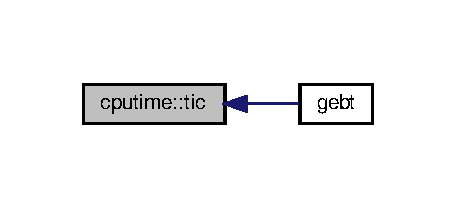
\includegraphics[width=219pt]{namespacecputime_a8ddcbcba17e66ece6b29c63b69753684_icgraph}
\end{center}
\end{figure}
\mbox{\Hypertarget{namespacecputime_a6c69d406a4397d16ea918e4eb035fde9}\label{namespacecputime_a6c69d406a4397d16ea918e4eb035fde9}} 
\index{cputime@{cputime}!toc@{toc}}
\index{toc@{toc}!cputime@{cputime}}
\subsubsection{\texorpdfstring{toc()}{toc()}}
{\footnotesize\ttfamily real function, public cputime\+::toc (\begin{DoxyParamCaption}{ }\end{DoxyParamCaption})}



Stop the timer. 

\begin{DoxyReturn}{Returns}
computation time (seconds) 
\end{DoxyReturn}


Definition at line 58 of file C\+P\+Utime.\+f90.

Here is the caller graph for this function\+:\nopagebreak
\begin{figure}[H]
\begin{center}
\leavevmode
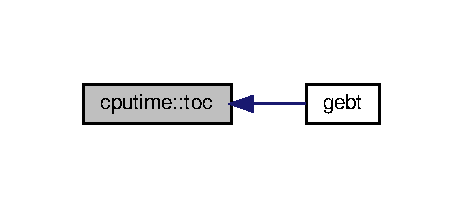
\includegraphics[width=222pt]{namespacecputime_a6c69d406a4397d16ea918e4eb035fde9_icgraph}
\end{center}
\end{figure}


\subsection{Variable Documentation}
\mbox{\Hypertarget{namespacecputime_ad2d439f12d6051a89b5ba23d52aa3e4f}\label{namespacecputime_ad2d439f12d6051a89b5ba23d52aa3e4f}} 
\index{cputime@{cputime}!finish@{finish}}
\index{finish@{finish}!cputime@{cputime}}
\subsubsection{\texorpdfstring{finish}{finish}}
{\footnotesize\ttfamily integer(8) cputime\+::finish\hspace{0.3cm}{\ttfamily [private]}}



Definition at line 31 of file C\+P\+Utime.\+f90.

\mbox{\Hypertarget{namespacecputime_a7648112eab2c70c19434f100a9599633}\label{namespacecputime_a7648112eab2c70c19434f100a9599633}} 
\index{cputime@{cputime}!rate@{rate}}
\index{rate@{rate}!cputime@{cputime}}
\subsubsection{\texorpdfstring{rate}{rate}}
{\footnotesize\ttfamily integer(8) cputime\+::rate\hspace{0.3cm}{\ttfamily [private]}}



Definition at line 31 of file C\+P\+Utime.\+f90.

\mbox{\Hypertarget{namespacecputime_a3c944d7fc4487f41daf6348bf28b1598}\label{namespacecputime_a3c944d7fc4487f41daf6348bf28b1598}} 
\index{cputime@{cputime}!start@{start}}
\index{start@{start}!cputime@{cputime}}
\subsubsection{\texorpdfstring{start}{start}}
{\footnotesize\ttfamily integer(8) cputime\+::start\hspace{0.3cm}{\ttfamily [private]}}



Definition at line 31 of file C\+P\+Utime.\+f90.


\hypertarget{namespaceeigenmumps}{}\section{eigenmumps Module Reference}
\label{namespaceeigenmumps}\index{eigenmumps@{eigenmumps}}


This module contains the main routines needed for eigen value analysis and allow to call Arpack and M\+U\+M\+PS library.  


\subsection*{Functions/\+Subroutines}
\begin{DoxyCompactItemize}
\item 
subroutine, public \hyperlink{namespaceeigenmumps_ae4a95ffe93412104411a9914edccd507}{eigensolvemumps} (ndof\+\_\+el, memb\+\_\+info, v\+\_\+root\+\_\+a, omega\+\_\+a, member, pt\+\_\+condition, niter, error, ncond\+\_\+mb, mb\+\_\+condition, distr\+\_\+fun, dof\+\_\+con, x, nev, eigen\+\_\+val, eigen\+\_\+vec, aero\+\_\+flag, grav\+\_\+flag)
\begin{DoxyCompactList}\small\item\em this routine solve the eigenproblem by linearising about a steady state x \end{DoxyCompactList}\item 
subroutine \hyperlink{namespaceeigenmumps_a86ca8fa64997377eaafa9b3b69a86d49}{arpack} (nev, ncv, er, ei, vector, error)
\begin{DoxyCompactList}\small\item\em this subroutine make the interface with the arpack sparse eigensolver library \end{DoxyCompactList}\item 
subroutine \hyperlink{namespaceeigenmumps_ac941735ba53914846bfec44d74ad79c6}{aw} (u, nzM, irnM, jcnM, coef\+\_\+mass, w)
\begin{DoxyCompactList}\small\item\em Solve the linear system K$\ast$V = Z to avoid matrix inversion with solver M\+U\+M\+PS. \end{DoxyCompactList}\end{DoxyCompactItemize}
\subsection*{Variables}
\begin{DoxyCompactItemize}
\item 
type(dmumps\+\_\+struc) \hyperlink{namespaceeigenmumps_a96a8141178a4cd84a24bd63b11685409}{mumps\+\_\+par}
\begin{DoxyCompactList}\small\item\em an array containing the configuration parameters of M\+U\+M\+PS solver \end{DoxyCompactList}\item 
integer \hyperlink{namespaceeigenmumps_a0b6d919fe610b180483db0dcba47ba1c}{ierr}
\begin{DoxyCompactList}\small\item\em error code of the M\+U\+M\+PS solver \end{DoxyCompactList}\end{DoxyCompactItemize}


\subsection{Detailed Description}
This module contains the main routines needed for eigen value analysis and allow to call Arpack and M\+U\+M\+PS library. 

\subsection{Function/\+Subroutine Documentation}
\mbox{\Hypertarget{namespaceeigenmumps_a86ca8fa64997377eaafa9b3b69a86d49}\label{namespaceeigenmumps_a86ca8fa64997377eaafa9b3b69a86d49}} 
\index{eigenmumps@{eigenmumps}!arpack@{arpack}}
\index{arpack@{arpack}!eigenmumps@{eigenmumps}}
\subsubsection{\texorpdfstring{arpack()}{arpack()}}
{\footnotesize\ttfamily subroutine eigenmumps\+::arpack (\begin{DoxyParamCaption}\item[{integer, intent(inout)}]{nev,  }\item[{integer, intent(in)}]{ncv,  }\item[{real(dbl), dimension(\+:), intent(out)}]{er,  }\item[{real(dbl), dimension(\+:), intent(out)}]{ei,  }\item[{real(dbl), dimension(\+:,\+:), intent(out)}]{vector,  }\item[{character($\ast$), intent(out)}]{error }\end{DoxyParamCaption})\hspace{0.3cm}{\ttfamily [private]}}



this subroutine make the interface with the arpack sparse eigensolver library 


\begin{DoxyParams}[1]{Parameters}
\mbox{\tt in,out}  & {\em nev} & \hyperlink{namespaceioaero_a1216c8699aea9eb27e3d795cc9d8d271}{ioaero\+::nev}\\
\hline
\mbox{\tt in}  & {\em ncv} & size of the subdomain used bye the I\+R\+AM algorithm (doc Arpack)\\
\hline
\mbox{\tt out}  & {\em error} & \hyperlink{namespaceioaero_aebd85ae2a176f49a7213d8ed7b68f887}{ioaero\+::error}\\
\hline
\mbox{\tt out}  & {\em er} & Real part of the eigenvalue (before problem inversion)\\
\hline
\mbox{\tt out}  & {\em ei} & Imaginary part of the eigenvalue (before problem inversion)\\
\hline
\mbox{\tt out}  & {\em vector} & eigenvector computed by arpack \\
\hline
\end{DoxyParams}


Definition at line 248 of file Eigen\+Solve\+Mumps.\+f90.

\mbox{\Hypertarget{namespaceeigenmumps_ac941735ba53914846bfec44d74ad79c6}\label{namespaceeigenmumps_ac941735ba53914846bfec44d74ad79c6}} 
\index{eigenmumps@{eigenmumps}!aw@{aw}}
\index{aw@{aw}!eigenmumps@{eigenmumps}}
\subsubsection{\texorpdfstring{aw()}{aw()}}
{\footnotesize\ttfamily subroutine eigenmumps\+::aw (\begin{DoxyParamCaption}\item[{real(dbl), dimension(nsize), intent(out)}]{u,  }\item[{integer, intent(in)}]{nzM,  }\item[{integer, dimension(\+:), intent(in)}]{irnM,  }\item[{integer, dimension(\+:), intent(in)}]{jcnM,  }\item[{real(dbl), dimension(\+:), intent(in)}]{coef\+\_\+mass,  }\item[{real(dbl), dimension(nsize), intent(in)}]{w }\end{DoxyParamCaption})\hspace{0.3cm}{\ttfamily [private]}}



Solve the linear system K$\ast$V = Z to avoid matrix inversion with solver M\+U\+M\+PS. 


\begin{DoxyParams}[1]{Parameters}
\mbox{\tt in}  & {\em nzm} & number of nonzero coefficient\\
\hline
\mbox{\tt in}  & {\em irnm} & line index of nonzero values\\
\hline
\mbox{\tt in}  & {\em jcnm} & column index of nonzero values\\
\hline
\mbox{\tt in}  & {\em coef\+\_\+mass} & mass matrix sparse coefficient\\
\hline
\mbox{\tt in}  & {\em w} & R\+HS vector\\
\hline
\mbox{\tt out}  & {\em u} & solution vector V \\
\hline
\end{DoxyParams}


Definition at line 357 of file Eigen\+Solve\+Mumps.\+f90.

\mbox{\Hypertarget{namespaceeigenmumps_ae4a95ffe93412104411a9914edccd507}\label{namespaceeigenmumps_ae4a95ffe93412104411a9914edccd507}} 
\index{eigenmumps@{eigenmumps}!eigensolvemumps@{eigensolvemumps}}
\index{eigensolvemumps@{eigensolvemumps}!eigenmumps@{eigenmumps}}
\subsubsection{\texorpdfstring{eigensolvemumps()}{eigensolvemumps()}}
{\footnotesize\ttfamily subroutine, public eigenmumps\+::eigensolvemumps (\begin{DoxyParamCaption}\item[{integer, intent(in)}]{ndof\+\_\+el,  }\item[{type (memberinf), dimension(\+:), intent(in)}]{memb\+\_\+info,  }\item[{real(dbl), dimension(\+:), intent(in)}]{v\+\_\+root\+\_\+a,  }\item[{real(dbl), dimension(\+:), intent(in)}]{omega\+\_\+a,  }\item[{integer, dimension(\+:,\+:), intent(in)}]{member,  }\item[{type(prescriinf), dimension(\+:), intent(in)}]{pt\+\_\+condition,  }\item[{integer, intent(in)}]{niter,  }\item[{character($\ast$), intent(out)}]{error,  }\item[{integer, intent(in)}]{ncond\+\_\+mb,  }\item[{type(prescriinf), dimension(\+:), intent(in)}]{mb\+\_\+condition,  }\item[{real(dbl), dimension(\+:,\+:), intent(in)}]{distr\+\_\+fun,  }\item[{integer, dimension(\+:)}]{dof\+\_\+con,  }\item[{real(dbl), dimension(\+:), intent(in)}]{x,  }\item[{integer, intent(inout)}]{nev,  }\item[{real(dbl), dimension(\+:,\+:), intent(out)}]{eigen\+\_\+val,  }\item[{real(dbl), dimension(\+:,\+:), intent(out)}]{eigen\+\_\+vec,  }\item[{integer, intent(in)}]{aero\+\_\+flag,  }\item[{integer, intent(in)}]{grav\+\_\+flag }\end{DoxyParamCaption})}



this routine solve the eigenproblem by linearising about a steady state x 


\begin{DoxyParams}[1]{Parameters}
\mbox{\tt in}  & {\em ndof\+\_\+el} & \hyperlink{namespaceioaero_a2b095b5cb5aab1f100d202c8004c9cb5}{ioaero\+::ndof\+\_\+el}\\
\hline
\mbox{\tt in}  & {\em aero\+\_\+flag} & \hyperlink{namespaceioaero_afb280b6ca8de323c9a07076df81a71e1}{ioaero\+::aero\+\_\+flag}\\
\hline
\mbox{\tt in}  & {\em grav\+\_\+flag} & \hyperlink{namespaceioaero_a831fe87d45ef05e3e29a8c4c2fc88c8f}{ioaero\+::grav\+\_\+flag}\\
\hline
\mbox{\tt in}  & {\em memb\+\_\+info} & array containing the characteristics of the beam members\\
\hline
\mbox{\tt in}  & {\em v\+\_\+root\+\_\+a} & linear velocity of frame a\\
\hline
\mbox{\tt in}  & {\em omega\+\_\+a} & angular velocity of frame a\\
\hline
\mbox{\tt in}  & {\em distr\+\_\+fun} & \hyperlink{namespaceioaero_a1d7c3689e30c2925cd403a84e9176242}{ioaero\+::distr\+\_\+fun}\\
\hline
\mbox{\tt in}  & {\em member} & \hyperlink{namespaceioaero_ae040b39fe109c45b001985415e230ec3}{ioaero\+::member}\\
\hline
\mbox{\tt in}  & {\em niter} & \hyperlink{namespaceioaero_ac008486fd12e0029a1ef77b3ca5e12c3}{ioaero\+::niter}\\
\hline
\mbox{\tt in}  & {\em ncond\+\_\+mb} & \hyperlink{namespaceioaero_ab9193f4ff70a22ae5858118fc653f22b}{ioaero\+::ncond\+\_\+mb}\\
\hline
\mbox{\tt in}  & {\em pt\+\_\+condition} & \hyperlink{namespaceioaero_a4344b2018135ae7fe0a09f4265fd2c29}{ioaero\+::pt\+\_\+condition}\\
\hline
\mbox{\tt in}  & {\em mb\+\_\+condition} & \hyperlink{namespaceioaero_a2463929ef049b49fe7b49011c66cc806}{ioaero\+::mb\+\_\+condition}\\
\hline
 & {\em dof\+\_\+con} & the connecting condition for key point.\\
\hline
\mbox{\tt out}  & {\em error} & \hyperlink{namespaceioaero_aebd85ae2a176f49a7213d8ed7b68f887}{ioaero\+::error}\\
\hline
\mbox{\tt in}  & {\em x} & the solution vector of the linear system (steady-\/state)\\
\hline
\mbox{\tt in,out}  & {\em nev} & \hyperlink{namespaceioaero_a1216c8699aea9eb27e3d795cc9d8d271}{ioaero\+::nev}\\
\hline
\mbox{\tt out}  & {\em eigen\+\_\+val} & \hyperlink{namespaceioaero_ae043619051217506f070ece6f24deedf}{ioaero\+::eigen\+\_\+val}\\
\hline
\mbox{\tt out}  & {\em eigen\+\_\+vec} & array containing the solution eigenvectors \\
\hline
\end{DoxyParams}


Definition at line 45 of file Eigen\+Solve\+Mumps.\+f90.



\subsection{Variable Documentation}
\mbox{\Hypertarget{namespaceeigenmumps_a0b6d919fe610b180483db0dcba47ba1c}\label{namespaceeigenmumps_a0b6d919fe610b180483db0dcba47ba1c}} 
\index{eigenmumps@{eigenmumps}!ierr@{ierr}}
\index{ierr@{ierr}!eigenmumps@{eigenmumps}}
\subsubsection{\texorpdfstring{ierr}{ierr}}
{\footnotesize\ttfamily integer eigenmumps\+::ierr}



error code of the M\+U\+M\+PS solver 



Definition at line 27 of file Eigen\+Solve\+Mumps.\+f90.

\mbox{\Hypertarget{namespaceeigenmumps_a96a8141178a4cd84a24bd63b11685409}\label{namespaceeigenmumps_a96a8141178a4cd84a24bd63b11685409}} 
\index{eigenmumps@{eigenmumps}!mumps\+\_\+par@{mumps\+\_\+par}}
\index{mumps\+\_\+par@{mumps\+\_\+par}!eigenmumps@{eigenmumps}}
\subsubsection{\texorpdfstring{mumps\+\_\+par}{mumps\_par}}
{\footnotesize\ttfamily type (dmumps\+\_\+struc) eigenmumps\+::mumps\+\_\+par}



an array containing the configuration parameters of M\+U\+M\+PS solver 



Definition at line 26 of file Eigen\+Solve\+Mumps.\+f90.


\hypertarget{namespaceelement}{}\section{element Module Reference}
\label{namespaceelement}\index{element@{element}}


This module contains information and calculation for an element within a member.  


\subsection*{Functions/\+Subroutines}
\begin{DoxyCompactItemize}
\item 
real(dbl) function, dimension(ndof\+\_\+el+ndof\+\_\+nd), public \hyperlink{namespaceelement_a267c29ec99208b5121ba2c6af7180016}{elemeqn} (ndof\+\_\+el)
\begin{DoxyCompactList}\small\item\em Compute the value of the Right Hand Side for a finite element. \end{DoxyCompactList}\item 
subroutine, public \hyperlink{namespaceelement_a172c175acb51f133e8b15a64c6e7f238}{elemjacobian} (ndof\+\_\+el, niter, elem\+Jac)
\begin{DoxyCompactList}\small\item\em Caculate the Jacobian matrix for each element. \end{DoxyCompactList}\item 
subroutine, public \hyperlink{namespaceelement_aeac4f943f8f4e225381fac5a1278d4eb}{elemmass} (ndof\+\_\+el, elemM)
\begin{DoxyCompactList}\small\item\em Caculate the mass matrix for each element. \end{DoxyCompactList}\item 
subroutine, public \hyperlink{namespaceelement_aa0f853882f2705c359567e433bb31fe9}{extractelementproperties} (elem\+\_\+no, memb\+\_\+info\+\_\+i, x\+\_\+elem, v\+\_\+root\+\_\+a, omega\+\_\+a, ndof\+\_\+el, init\+\_\+elem, aero\+\_\+flag, grav\+\_\+flag)
\begin{DoxyCompactList}\small\item\em Extract element properties needed for element assembly. \end{DoxyCompactList}\end{DoxyCompactItemize}
\subsection*{Variables}
\begin{DoxyCompactItemize}
\item 
real(dbl) \hyperlink{namespaceelement_a2ba7b882a33de416921d1a35d3a5e23a}{dl}
\begin{DoxyCompactList}\small\item\em length of the element \end{DoxyCompactList}\item 
real(dbl) \hyperlink{namespaceelement_a10e7976ce4185b147c590f281b7691b1}{le}
\begin{DoxyCompactList}\small\item\em the ending arc length of the current element \end{DoxyCompactList}\item 
real(dbl), dimension(ndim, ndim) \hyperlink{namespaceelement_a235dfda3fd31cfbf932e5a7cba3d18ec}{ecab}
\begin{DoxyCompactList}\small\item\em direction cosine matrix of the undeformed element \end{DoxyCompactList}\item 
real(dbl), dimension(nstrn, nstrn) \hyperlink{namespaceelement_a5cd41224c84f496a89d157c781b0d207}{eflex}
\begin{DoxyCompactList}\small\item\em flexibility matrix of the elment \end{DoxyCompactList}\item 
real(dbl), dimension(nstrn, nstrn) \hyperlink{namespaceelement_acd7a12a677d8157d3f792f2090fd0664}{emass}
\begin{DoxyCompactList}\small\item\em inverse of the mass matrix of the element \end{DoxyCompactList}\item 
type(distriload), public \hyperlink{namespaceelement_a99d2f733169debb6f9d7d8b30fbc49c4}{load}
\begin{DoxyCompactList}\small\item\em distributed load \end{DoxyCompactList}\item 
logical, public \hyperlink{namespaceelement_a4fecf0570d257bca42bf4ece885f4721}{exist\+\_\+load}
\item 
logical, public \hyperlink{namespaceelement_a2babdd1ffcf39971fb9b118d88d1e223}{follower\+\_\+load}
\begin{DoxyCompactList}\small\item\em flags to indicate whether distributed load exist and whether they are follower forces \end{DoxyCompactList}\item 
real(dbl), dimension(ndim) \hyperlink{namespaceelement_ad1b3c2d05a1c131831f0d4eef43f9105}{ui}
\item 
real(dbl), dimension(ndim) \hyperlink{namespaceelement_ac0a8fcda10d1b0af47fd7d713ebcd5fe}{theta}
\item 
real(dbl), dimension(ndim) \hyperlink{namespaceelement_aa97de262111f37b6e4b721cad221946a}{fi}
\item 
real(dbl), dimension(ndim) \hyperlink{namespaceelement_aaa8af943c974b60b3eeacd9ea685f28b}{mi}
\item 
real(dbl), dimension(ndim) \hyperlink{namespaceelement_aa1c0af00208b47c11ed5b1dc17fb33b3}{e1gammad}
\item 
real(dbl), dimension(ndim) \hyperlink{namespaceelement_ad5ea7346491c313bb4094d1838fe747e}{kappa}
\item 
real(dbl), dimension(ndim) \hyperlink{namespaceelement_afd7049cf1988fff1d20ea9fae6290b27}{epi}
\item 
real(dbl), dimension(ndim) \hyperlink{namespaceelement_aec782f88829f63bff819c43e9c19f02c}{hi}
\item 
real(dbl), dimension(ndim) \hyperlink{namespaceelement_a7e7198874f6dd0702abdd8ba0dfc7c2d}{vi}
\item 
real(dbl), dimension(ndim) \hyperlink{namespaceelement_ad819facefa1f1184a10576007ac79ba4}{omegai}
\item 
real(dbl), dimension(ndim) \hyperlink{namespaceelement_a38ecc4368e8e51d5672ad47f1a79536e}{ev\+\_\+i}
\begin{DoxyCompactList}\small\item\em initial velocity of the mid point of the element \end{DoxyCompactList}\item 
real(dbl), dimension(ndim) \hyperlink{namespaceelement_a8d354f7c393ef7f0ba4144a20b5390ba}{eomega\+\_\+a}
\begin{DoxyCompactList}\small\item\em initial angular velocity of the element \end{DoxyCompactList}\item 
real(dbl), dimension(ndim, ndim) \hyperlink{namespaceelement_a355b3273dce5e581cf75d079f4f4557d}{ect}
\begin{DoxyCompactList}\small\item\em the transpose of the direction cosine matrix corresponding to elastic rotation \end{DoxyCompactList}\item 
real(dbl), dimension(ndim, ndim) \hyperlink{namespaceelement_a94c9e7eb21bc71af7de19ee37093b959}{ectcab}
\begin{DoxyCompactList}\small\item\em e\+C\+T.\+Cab \end{DoxyCompactList}\item 
real(dbl), dimension(ndim, ndim) \hyperlink{namespaceelement_af027b6db49efde36e310bc9e4f8e0d06}{ecabhalfl}
\begin{DoxyCompactList}\small\item\em e\+Cab$\ast$d\+L/2 \end{DoxyCompactList}\item 
real(dbl), dimension(ndim, ndim) \hyperlink{namespaceelement_afa3adc34db2cdcd479dd21a3873ef5d1}{ectcabhalfl}
\begin{DoxyCompactList}\small\item\em e\+C\+T\+Cab$\ast$d\+L/2 \end{DoxyCompactList}\item 
real(dbl), dimension(ndim) \hyperlink{namespaceelement_a0ceabdb65183ba09653081ad8ca4259d}{uidot}
\item 
real(dbl), dimension(ndim) \hyperlink{namespaceelement_a7404d160f35ff4cfc4ea3e3d8f76cb89}{thetadot}
\item 
real(dbl), dimension(ndim) \hyperlink{namespaceelement_a8dd69dbb67c325d43811863c2f95e9e0}{ctcabpdot}
\item 
real(dbl), dimension(ndim) \hyperlink{namespaceelement_a4afdc10a9e39215ab6c7d03fe10a4473}{ctcabhdot}
\item 
real(dbl) \hyperlink{namespaceelement_a3c256e3e6f1a658f469f77ed8f7d033e}{rho}
\item 
real(dbl) \hyperlink{namespaceelement_a55d26e2f0da1242eeb9cc8d3d589f1e5}{chord}
\item 
real(dbl) \hyperlink{namespaceelement_aa46e16e8787633edb4e4c0c8c6809ecb}{x\+\_\+cg}
\item 
real(dbl) \hyperlink{namespaceelement_aa45829429fe33aa2b5cd6feaacc2c739}{alpha}
\item 
real(dbl) \hyperlink{namespaceelement_ac749aa20088ae7c80700929a64803dfe}{alphadot}
\item 
real(dbl) \hyperlink{namespaceelement_a50a818b525bc9fc33afce618163cb17e}{hdot}
\item 
real(dbl) \hyperlink{namespaceelement_a3a0a4401f2461a4b65f656a9af6e23d8}{aw}
\item 
real(dbl) \hyperlink{namespaceelement_af3dda698afcf40c00ff5008dc5f3da36}{bw}
\item 
real(dbl) \hyperlink{namespaceelement_a6d48ee96f674959ef1225a3730fcf3e7}{u}
\item 
real(dbl) \hyperlink{namespaceelement_a012a2b1125e535b957a6be4ea842da6d}{hdotdot}
\item 
real(dbl) \hyperlink{namespaceelement_a3b4df4c1043c9ebd56f5d23ca24d00ac}{alphadotdot}
\item 
real(dbl) \hyperlink{namespaceelement_aab90697519f32a9a4f56786465c1bd0b}{alpha\+\_\+ac}
\item 
real(dbl) \hyperlink{namespaceelement_a9ab0720aafb3053cad927fc402be3000}{beta\+\_\+ac}
\item 
real(dbl) \hyperlink{namespaceelement_a1ea3f00156313fce1a3de0a00499702c}{beta}
\item 
integer \hyperlink{namespaceelement_a17661475127df7ce4d09fb1e942cbd58}{a\+\_\+flag}
\item 
integer \hyperlink{namespaceelement_a4f9b46e901684a30dec91ad363247dd3}{g\+\_\+flag}
\item 
real(dbl), dimension(nstates) \hyperlink{namespaceelement_abfc6a3777c98caf9d75aa0fa4ce97e17}{lambda}
\item 
real(dbl), dimension(nstates) \hyperlink{namespaceelement_a627873fe5856f3a9c95039d8f6877039}{lambdadot}
\item 
real(dbl), dimension(nstates, 2 $\ast$nstates+2) \hyperlink{namespaceelement_abf487a07f5188539bf21883fc0a10c70}{p}
\item 
real(dbl), dimension(nstates, nstates) \hyperlink{namespaceelement_af575d84cfbaeca87aec268f375efac06}{ident}
\item 
real(dbl) \hyperlink{namespaceelement_aa9695f47555869b8d547d0d87d49275e}{lambda0}
\item 
real(dbl), dimension(nstates, nstates) \hyperlink{namespaceelement_ad0c7d68510d195a504efc593e729263f}{a}
\item 
real(dbl), dimension(nstates) \hyperlink{namespaceelement_a031bf1cdfa87524ec1b508c44f537002}{b}
\item 
real(dbl), dimension(nstates) \hyperlink{namespaceelement_a1203577a202409830d687bf3b68c621e}{c}
\item 
real(dbl), dimension(ndim) \hyperlink{namespaceelement_a88c83da354d518bfd81c3ef7691b4682}{dir\+\_\+moment}
\item 
real(dbl), dimension(ndim) \hyperlink{namespaceelement_a10ce0718ec68d00dd9fab0c290410366}{dir\+\_\+lift}
\item 
real(dbl), dimension(ndim, ndim) \hyperlink{namespaceelement_a1dcc074ceaab61da55e1b1964ea3d235}{jdir\+\_\+moment}
\item 
real(dbl), dimension(ndim, ndim) \hyperlink{namespaceelement_a580ce3f83ad83383203449b2d8f4a3a4}{jdir\+\_\+lift}
\item 
real(dbl), dimension(ndim) \hyperlink{namespaceelement_a38bfdfabd1e6c253836e6fb02c0d6784}{jalpha\+\_\+theta}
\item 
real(dbl), dimension(ndim) \hyperlink{namespaceelement_a6c09852dc997af8b311d0ced2855794d}{jalphadot\+\_\+theta}
\item 
real(dbl), dimension(ndim) \hyperlink{namespaceelement_a8fc86f2f6fcef7f4b4216181ed52a8b7}{jhdot\+\_\+theta}
\item 
real(dbl), dimension(ndim+ndim) \hyperlink{namespaceelement_a21fa4f1bba2c9d7c57ba982869fe0a95}{jalphadot\+\_\+ph}
\item 
real(dbl), dimension(ndim+ndim) \hyperlink{namespaceelement_a9ef70f6658a771b1ae6491475da5f9c3}{jhdot\+\_\+ph}
\item 
real(dbl), dimension(ndim+ndim) \hyperlink{namespaceelement_ab9d2421c52f64e5ff0b10858aca6bd43}{jalphadotdot\+\_\+phdot}
\item 
real(dbl), dimension(ndim+ndim) \hyperlink{namespaceelement_a0928be80ffe200a8be069851f2c20dbd}{jhdotdot\+\_\+phdot}
\item 
real(dbl), dimension(ndim+ndim) \hyperlink{namespaceelement_a098f0887e0821d48cc06e45f446b9aab}{jalphadotdot\+\_\+ph}
\item 
real(dbl), dimension(ndim+ndim) \hyperlink{namespaceelement_a2ce32735f66193668003049e1cf17d61}{jhdotdot\+\_\+ph}
\item 
real(dbl), dimension(ndim+ndim) \hyperlink{namespaceelement_a7c62d3aab34ad67ea920d7293726205e}{jlambda0\+\_\+phdot}
\item 
real(dbl), dimension(nstates) \hyperlink{namespaceelement_abb09debf79a65110c87abb4892423e00}{jlambda0\+\_\+lambda}
\item 
real(dbl), dimension(3, 18+nstates) \hyperlink{namespaceelement_a2cc8d4739c02a1302e8c31d681c70eb8}{jlift}
\item 
real(dbl), dimension(3, 18+nstates) \hyperlink{namespaceelement_ac6e33874e30f493a8e29de4f0c87af0a}{jmoment}
\item 
real(dbl), dimension(ndim, ndim) \hyperlink{namespaceelement_a8cf9df9304438d7eaddcd8609c6968c5}{ecaf}
\item 
real(dbl), dimension(ndim) \hyperlink{namespaceelement_aeced564b191f69b1327f9b9164f371f5}{wind}
\end{DoxyCompactItemize}


\subsection{Detailed Description}
This module contains information and calculation for an element within a member. 

\subsection{Function/\+Subroutine Documentation}
\mbox{\Hypertarget{namespaceelement_a267c29ec99208b5121ba2c6af7180016}\label{namespaceelement_a267c29ec99208b5121ba2c6af7180016}} 
\index{element@{element}!elemeqn@{elemeqn}}
\index{elemeqn@{elemeqn}!element@{element}}
\subsubsection{\texorpdfstring{elemeqn()}{elemeqn()}}
{\footnotesize\ttfamily real(dbl) function, dimension(ndof\+\_\+el+ndof\+\_\+nd), public element\+::elemeqn (\begin{DoxyParamCaption}\item[{integer, intent(in)}]{ndof\+\_\+el }\end{DoxyParamCaption})}



Compute the value of the Right Hand Side for a finite element. 


\begin{DoxyParams}[1]{Parameters}
\mbox{\tt in}  & {\em ndof\+\_\+el} & \hyperlink{namespaceioaero_a2b095b5cb5aab1f100d202c8004c9cb5}{ioaero\+::ndof\+\_\+el} \\
\hline
\end{DoxyParams}


Definition at line 79 of file Element.\+f90.

Here is the caller graph for this function\+:\nopagebreak
\begin{figure}[H]
\begin{center}
\leavevmode
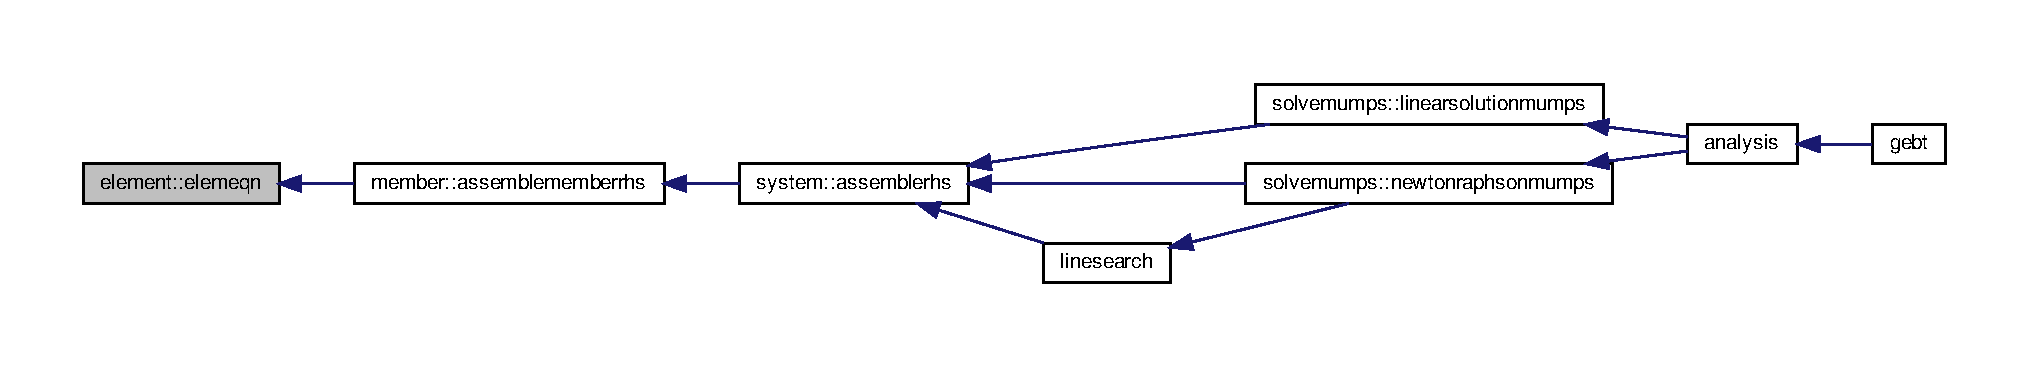
\includegraphics[width=350pt]{namespaceelement_a267c29ec99208b5121ba2c6af7180016_icgraph}
\end{center}
\end{figure}
\mbox{\Hypertarget{namespaceelement_a172c175acb51f133e8b15a64c6e7f238}\label{namespaceelement_a172c175acb51f133e8b15a64c6e7f238}} 
\index{element@{element}!elemjacobian@{elemjacobian}}
\index{elemjacobian@{elemjacobian}!element@{element}}
\subsubsection{\texorpdfstring{elemjacobian()}{elemjacobian()}}
{\footnotesize\ttfamily subroutine, public element\+::elemjacobian (\begin{DoxyParamCaption}\item[{integer, intent(in)}]{ndof\+\_\+el,  }\item[{integer, intent(in)}]{niter,  }\item[{real(dbl), dimension(\+:,\+:), intent(out)}]{elem\+Jac }\end{DoxyParamCaption})}



Caculate the Jacobian matrix for each element. 


\begin{DoxyParams}[1]{Parameters}
\mbox{\tt in}  & {\em ndof\+\_\+el} & \hyperlink{namespaceioaero_a2b095b5cb5aab1f100d202c8004c9cb5}{ioaero\+::ndof\+\_\+el}\\
\hline
\mbox{\tt in}  & {\em niter} & \hyperlink{namespaceioaero_ac008486fd12e0029a1ef77b3ca5e12c3}{ioaero\+::niter}\\
\hline
\mbox{\tt out}  & {\em elemjac} & the coefficient matrix for each element \\
\hline
\end{DoxyParams}


Definition at line 209 of file Element.\+f90.

Here is the caller graph for this function\+:\nopagebreak
\begin{figure}[H]
\begin{center}
\leavevmode
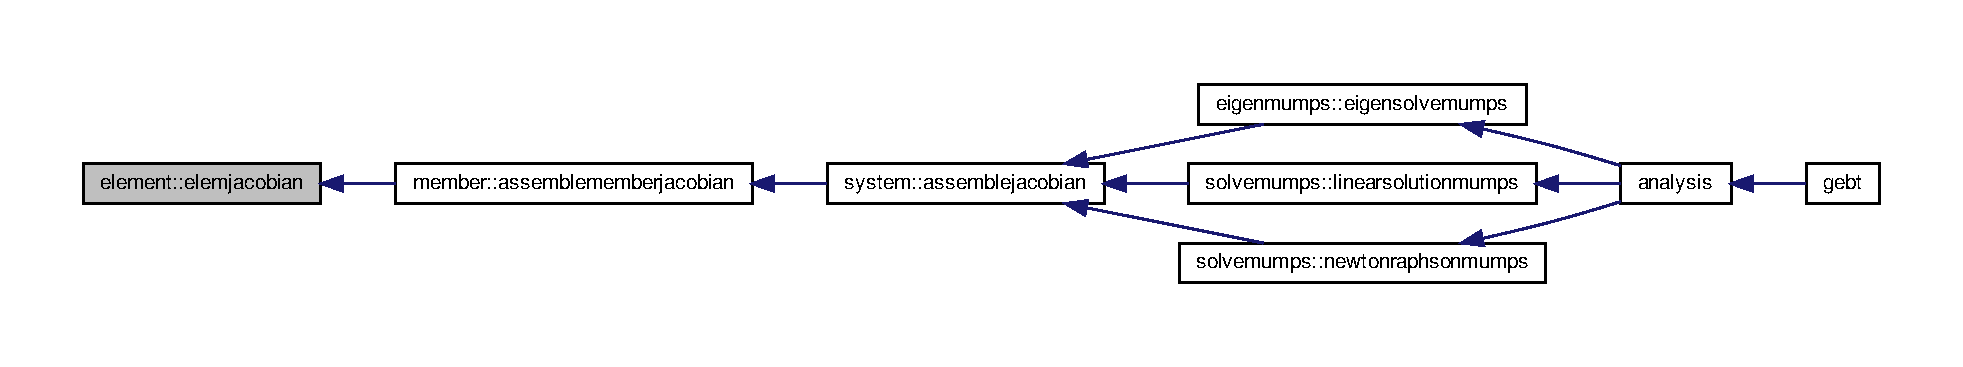
\includegraphics[width=350pt]{namespaceelement_a172c175acb51f133e8b15a64c6e7f238_icgraph}
\end{center}
\end{figure}
\mbox{\Hypertarget{namespaceelement_aeac4f943f8f4e225381fac5a1278d4eb}\label{namespaceelement_aeac4f943f8f4e225381fac5a1278d4eb}} 
\index{element@{element}!elemmass@{elemmass}}
\index{elemmass@{elemmass}!element@{element}}
\subsubsection{\texorpdfstring{elemmass()}{elemmass()}}
{\footnotesize\ttfamily subroutine, public element\+::elemmass (\begin{DoxyParamCaption}\item[{integer, intent(in)}]{ndof\+\_\+el,  }\item[{real(dbl), dimension(\+:,\+:), intent(out)}]{elemM }\end{DoxyParamCaption})}



Caculate the mass matrix for each element. 


\begin{DoxyParams}[1]{Parameters}
\mbox{\tt in}  & {\em ndof\+\_\+el} & \hyperlink{namespaceioaero_a2b095b5cb5aab1f100d202c8004c9cb5}{ioaero\+::ndof\+\_\+el}\\
\hline
\mbox{\tt out}  & {\em elemm} & the mass matrix for each element \\
\hline
\end{DoxyParams}


Definition at line 487 of file Element.\+f90.

Here is the caller graph for this function\+:\nopagebreak
\begin{figure}[H]
\begin{center}
\leavevmode
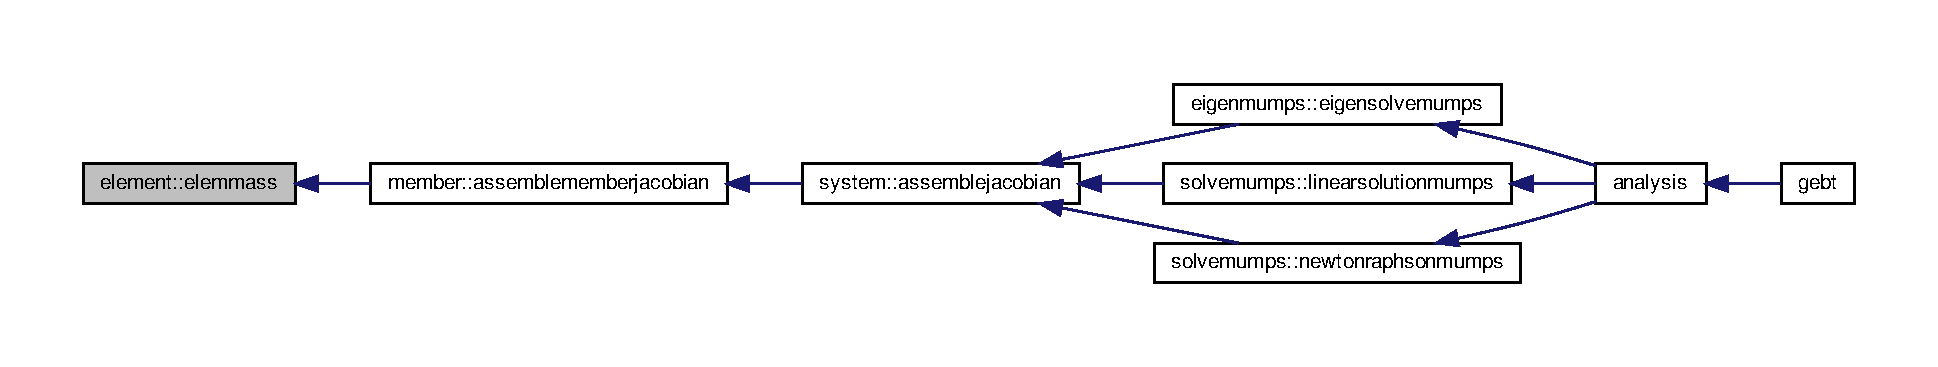
\includegraphics[width=350pt]{namespaceelement_aeac4f943f8f4e225381fac5a1278d4eb_icgraph}
\end{center}
\end{figure}
\mbox{\Hypertarget{namespaceelement_aa0f853882f2705c359567e433bb31fe9}\label{namespaceelement_aa0f853882f2705c359567e433bb31fe9}} 
\index{element@{element}!extractelementproperties@{extractelementproperties}}
\index{extractelementproperties@{extractelementproperties}!element@{element}}
\subsubsection{\texorpdfstring{extractelementproperties()}{extractelementproperties()}}
{\footnotesize\ttfamily subroutine, public element\+::extractelementproperties (\begin{DoxyParamCaption}\item[{integer, intent(in)}]{elem\+\_\+no,  }\item[{type (memberinf), intent(in)}]{memb\+\_\+info\+\_\+i,  }\item[{real(dbl), dimension(\+:), intent(in)}]{x\+\_\+elem,  }\item[{real(dbl), dimension(\+:), intent(in)}]{v\+\_\+root\+\_\+a,  }\item[{real(dbl), dimension(\+:), intent(in)}]{omega\+\_\+a,  }\item[{integer, intent(in)}]{ndof\+\_\+el,  }\item[{real(dbl), dimension(\+:,\+:), intent(inout)}]{init\+\_\+elem,  }\item[{integer, intent(in)}]{aero\+\_\+flag,  }\item[{integer, intent(in)}]{grav\+\_\+flag }\end{DoxyParamCaption})}



Extract element properties needed for element assembly. 


\begin{DoxyParams}[1]{Parameters}
\mbox{\tt in}  & {\em elem\+\_\+no} & Element index\\
\hline
\mbox{\tt in}  & {\em memb\+\_\+info\+\_\+i} & the paramater of the members (see memberinf Type)\\
\hline
\mbox{\tt in}  & {\em x\+\_\+elem} & the 12 variables of the element u\+\_\+i, , F\+\_\+i, M\+\_\+i, for dynamic analysis, 6 more Pi, Hi. for initial step, x\+\_\+elem contains, C\+T\+Cab\+Pdot, C\+T\+Cab\+Hdot, F\+\_\+i, M\+\_\+i, P\+\_\+i, H\+\_\+i. Finally for Peters aero the Ns induced flow states\\
\hline
\mbox{\tt in}  & {\em v\+\_\+root\+\_\+a} & linear velocity of the root point in inertial frame\\
\hline
\mbox{\tt in}  & {\em omega\+\_\+a} & angular velocity of the root point in inertial frame\\
\hline
\mbox{\tt in,out}  & {\em init\+\_\+elem} & initial step\+: the 12 initial values of the element u\+\_\+i, $ \theta_i, \dot{u}_i, \dot{theta}_i.$ Time marching\+: $2/dt ui+\dot{u}_i, 2/dt thetai+\dot{theta}_i, 2/dt CTCabP+\dot, 2/dt CTCabP+dot $\\
\hline
\mbox{\tt in}  & {\em ndof\+\_\+el} & \#ioaero\+::nedof\+\_\+el\\
\hline
\mbox{\tt in}  & {\em aero\+\_\+flag} & \hyperlink{namespaceioaero_afb280b6ca8de323c9a07076df81a71e1}{ioaero\+::aero\+\_\+flag}\\
\hline
\mbox{\tt in}  & {\em grav\+\_\+flag} & \hyperlink{namespaceioaero_a831fe87d45ef05e3e29a8c4c2fc88c8f}{ioaero\+::grav\+\_\+flag} \\
\hline
\end{DoxyParams}


Definition at line 616 of file Element.\+f90.

Here is the caller graph for this function\+:\nopagebreak
\begin{figure}[H]
\begin{center}
\leavevmode
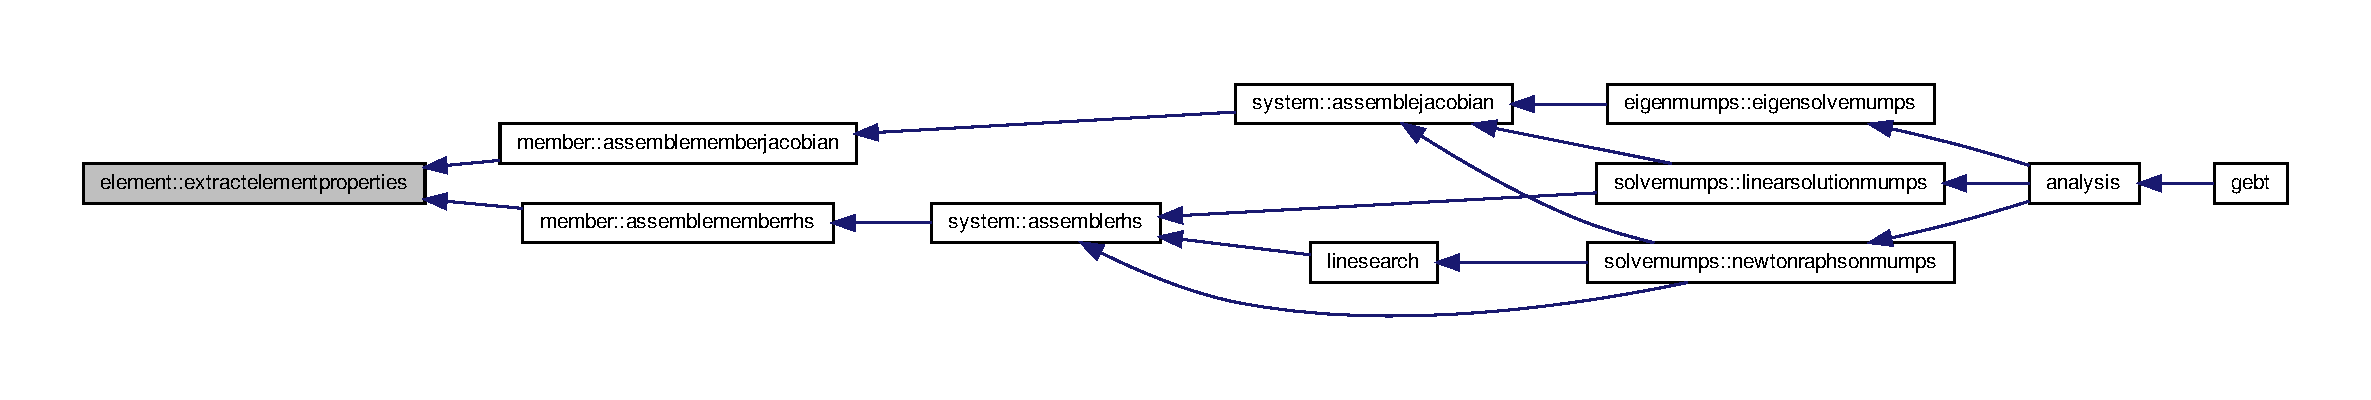
\includegraphics[width=350pt]{namespaceelement_aa0f853882f2705c359567e433bb31fe9_icgraph}
\end{center}
\end{figure}


\subsection{Variable Documentation}
\mbox{\Hypertarget{namespaceelement_ad0c7d68510d195a504efc593e729263f}\label{namespaceelement_ad0c7d68510d195a504efc593e729263f}} 
\index{element@{element}!a@{a}}
\index{a@{a}!element@{element}}
\subsubsection{\texorpdfstring{a}{a}}
{\footnotesize\ttfamily real(dbl), dimension(nstates,nstates) element\+::a\hspace{0.3cm}{\ttfamily [private]}}



Definition at line 56 of file Element.\+f90.

\mbox{\Hypertarget{namespaceelement_a17661475127df7ce4d09fb1e942cbd58}\label{namespaceelement_a17661475127df7ce4d09fb1e942cbd58}} 
\index{element@{element}!a\+\_\+flag@{a\+\_\+flag}}
\index{a\+\_\+flag@{a\+\_\+flag}!element@{element}}
\subsubsection{\texorpdfstring{a\+\_\+flag}{a\_flag}}
{\footnotesize\ttfamily integer element\+::a\+\_\+flag\hspace{0.3cm}{\ttfamily [private]}}



Definition at line 52 of file Element.\+f90.

\mbox{\Hypertarget{namespaceelement_aa45829429fe33aa2b5cd6feaacc2c739}\label{namespaceelement_aa45829429fe33aa2b5cd6feaacc2c739}} 
\index{element@{element}!alpha@{alpha}}
\index{alpha@{alpha}!element@{element}}
\subsubsection{\texorpdfstring{alpha}{alpha}}
{\footnotesize\ttfamily real(dbl) element\+::alpha\hspace{0.3cm}{\ttfamily [private]}}



Definition at line 51 of file Element.\+f90.

\mbox{\Hypertarget{namespaceelement_aab90697519f32a9a4f56786465c1bd0b}\label{namespaceelement_aab90697519f32a9a4f56786465c1bd0b}} 
\index{element@{element}!alpha\+\_\+ac@{alpha\+\_\+ac}}
\index{alpha\+\_\+ac@{alpha\+\_\+ac}!element@{element}}
\subsubsection{\texorpdfstring{alpha\+\_\+ac}{alpha\_ac}}
{\footnotesize\ttfamily real(dbl) element\+::alpha\+\_\+ac\hspace{0.3cm}{\ttfamily [private]}}



Definition at line 51 of file Element.\+f90.

\mbox{\Hypertarget{namespaceelement_ac749aa20088ae7c80700929a64803dfe}\label{namespaceelement_ac749aa20088ae7c80700929a64803dfe}} 
\index{element@{element}!alphadot@{alphadot}}
\index{alphadot@{alphadot}!element@{element}}
\subsubsection{\texorpdfstring{alphadot}{alphadot}}
{\footnotesize\ttfamily real(dbl) element\+::alphadot\hspace{0.3cm}{\ttfamily [private]}}



Definition at line 51 of file Element.\+f90.

\mbox{\Hypertarget{namespaceelement_a3b4df4c1043c9ebd56f5d23ca24d00ac}\label{namespaceelement_a3b4df4c1043c9ebd56f5d23ca24d00ac}} 
\index{element@{element}!alphadotdot@{alphadotdot}}
\index{alphadotdot@{alphadotdot}!element@{element}}
\subsubsection{\texorpdfstring{alphadotdot}{alphadotdot}}
{\footnotesize\ttfamily real(dbl) element\+::alphadotdot\hspace{0.3cm}{\ttfamily [private]}}



Definition at line 51 of file Element.\+f90.

\mbox{\Hypertarget{namespaceelement_a3a0a4401f2461a4b65f656a9af6e23d8}\label{namespaceelement_a3a0a4401f2461a4b65f656a9af6e23d8}} 
\index{element@{element}!aw@{aw}}
\index{aw@{aw}!element@{element}}
\subsubsection{\texorpdfstring{aw}{aw}}
{\footnotesize\ttfamily real(dbl) element\+::aw\hspace{0.3cm}{\ttfamily [private]}}



Definition at line 51 of file Element.\+f90.

\mbox{\Hypertarget{namespaceelement_a031bf1cdfa87524ec1b508c44f537002}\label{namespaceelement_a031bf1cdfa87524ec1b508c44f537002}} 
\index{element@{element}!b@{b}}
\index{b@{b}!element@{element}}
\subsubsection{\texorpdfstring{b}{b}}
{\footnotesize\ttfamily real(dbl), dimension(nstates) element\+::b\hspace{0.3cm}{\ttfamily [private]}}



Definition at line 56 of file Element.\+f90.

\mbox{\Hypertarget{namespaceelement_a1ea3f00156313fce1a3de0a00499702c}\label{namespaceelement_a1ea3f00156313fce1a3de0a00499702c}} 
\index{element@{element}!beta@{beta}}
\index{beta@{beta}!element@{element}}
\subsubsection{\texorpdfstring{beta}{beta}}
{\footnotesize\ttfamily real(dbl) element\+::beta\hspace{0.3cm}{\ttfamily [private]}}



Definition at line 51 of file Element.\+f90.

\mbox{\Hypertarget{namespaceelement_a9ab0720aafb3053cad927fc402be3000}\label{namespaceelement_a9ab0720aafb3053cad927fc402be3000}} 
\index{element@{element}!beta\+\_\+ac@{beta\+\_\+ac}}
\index{beta\+\_\+ac@{beta\+\_\+ac}!element@{element}}
\subsubsection{\texorpdfstring{beta\+\_\+ac}{beta\_ac}}
{\footnotesize\ttfamily real(dbl) element\+::beta\+\_\+ac\hspace{0.3cm}{\ttfamily [private]}}



Definition at line 51 of file Element.\+f90.

\mbox{\Hypertarget{namespaceelement_af3dda698afcf40c00ff5008dc5f3da36}\label{namespaceelement_af3dda698afcf40c00ff5008dc5f3da36}} 
\index{element@{element}!bw@{bw}}
\index{bw@{bw}!element@{element}}
\subsubsection{\texorpdfstring{bw}{bw}}
{\footnotesize\ttfamily real(dbl) element\+::bw\hspace{0.3cm}{\ttfamily [private]}}



Definition at line 51 of file Element.\+f90.

\mbox{\Hypertarget{namespaceelement_a1203577a202409830d687bf3b68c621e}\label{namespaceelement_a1203577a202409830d687bf3b68c621e}} 
\index{element@{element}!c@{c}}
\index{c@{c}!element@{element}}
\subsubsection{\texorpdfstring{c}{c}}
{\footnotesize\ttfamily real(dbl), dimension(nstates) element\+::c\hspace{0.3cm}{\ttfamily [private]}}



Definition at line 56 of file Element.\+f90.

\mbox{\Hypertarget{namespaceelement_a55d26e2f0da1242eeb9cc8d3d589f1e5}\label{namespaceelement_a55d26e2f0da1242eeb9cc8d3d589f1e5}} 
\index{element@{element}!chord@{chord}}
\index{chord@{chord}!element@{element}}
\subsubsection{\texorpdfstring{chord}{chord}}
{\footnotesize\ttfamily real(dbl) element\+::chord\hspace{0.3cm}{\ttfamily [private]}}



Definition at line 51 of file Element.\+f90.

\mbox{\Hypertarget{namespaceelement_a4afdc10a9e39215ab6c7d03fe10a4473}\label{namespaceelement_a4afdc10a9e39215ab6c7d03fe10a4473}} 
\index{element@{element}!ctcabhdot@{ctcabhdot}}
\index{ctcabhdot@{ctcabhdot}!element@{element}}
\subsubsection{\texorpdfstring{ctcabhdot}{ctcabhdot}}
{\footnotesize\ttfamily real(dbl), dimension(ndim) element\+::ctcabhdot\hspace{0.3cm}{\ttfamily [private]}}



Definition at line 48 of file Element.\+f90.

\mbox{\Hypertarget{namespaceelement_a8dd69dbb67c325d43811863c2f95e9e0}\label{namespaceelement_a8dd69dbb67c325d43811863c2f95e9e0}} 
\index{element@{element}!ctcabpdot@{ctcabpdot}}
\index{ctcabpdot@{ctcabpdot}!element@{element}}
\subsubsection{\texorpdfstring{ctcabpdot}{ctcabpdot}}
{\footnotesize\ttfamily real(dbl), dimension(ndim) element\+::ctcabpdot\hspace{0.3cm}{\ttfamily [private]}}



Definition at line 48 of file Element.\+f90.

\mbox{\Hypertarget{namespaceelement_a10ce0718ec68d00dd9fab0c290410366}\label{namespaceelement_a10ce0718ec68d00dd9fab0c290410366}} 
\index{element@{element}!dir\+\_\+lift@{dir\+\_\+lift}}
\index{dir\+\_\+lift@{dir\+\_\+lift}!element@{element}}
\subsubsection{\texorpdfstring{dir\+\_\+lift}{dir\_lift}}
{\footnotesize\ttfamily real(dbl), dimension(ndim) element\+::dir\+\_\+lift\hspace{0.3cm}{\ttfamily [private]}}



Definition at line 57 of file Element.\+f90.

\mbox{\Hypertarget{namespaceelement_a88c83da354d518bfd81c3ef7691b4682}\label{namespaceelement_a88c83da354d518bfd81c3ef7691b4682}} 
\index{element@{element}!dir\+\_\+moment@{dir\+\_\+moment}}
\index{dir\+\_\+moment@{dir\+\_\+moment}!element@{element}}
\subsubsection{\texorpdfstring{dir\+\_\+moment}{dir\_moment}}
{\footnotesize\ttfamily real(dbl), dimension(ndim) element\+::dir\+\_\+moment\hspace{0.3cm}{\ttfamily [private]}}



Definition at line 57 of file Element.\+f90.

\mbox{\Hypertarget{namespaceelement_a2ba7b882a33de416921d1a35d3a5e23a}\label{namespaceelement_a2ba7b882a33de416921d1a35d3a5e23a}} 
\index{element@{element}!dl@{dl}}
\index{dl@{dl}!element@{element}}
\subsubsection{\texorpdfstring{dl}{dl}}
{\footnotesize\ttfamily real(dbl) element\+::dl\hspace{0.3cm}{\ttfamily [private]}}



length of the element 



Definition at line 31 of file Element.\+f90.

\mbox{\Hypertarget{namespaceelement_aa1c0af00208b47c11ed5b1dc17fb33b3}\label{namespaceelement_aa1c0af00208b47c11ed5b1dc17fb33b3}} 
\index{element@{element}!e1gammad@{e1gammad}}
\index{e1gammad@{e1gammad}!element@{element}}
\subsubsection{\texorpdfstring{e1gammad}{e1gammad}}
{\footnotesize\ttfamily real(dbl), dimension(ndim) element\+::e1gammad\hspace{0.3cm}{\ttfamily [private]}}



Definition at line 39 of file Element.\+f90.

\mbox{\Hypertarget{namespaceelement_a235dfda3fd31cfbf932e5a7cba3d18ec}\label{namespaceelement_a235dfda3fd31cfbf932e5a7cba3d18ec}} 
\index{element@{element}!ecab@{ecab}}
\index{ecab@{ecab}!element@{element}}
\subsubsection{\texorpdfstring{ecab}{ecab}}
{\footnotesize\ttfamily real(dbl), dimension(ndim,ndim) element\+::ecab\hspace{0.3cm}{\ttfamily [private]}}



direction cosine matrix of the undeformed element 



Definition at line 33 of file Element.\+f90.

\mbox{\Hypertarget{namespaceelement_af027b6db49efde36e310bc9e4f8e0d06}\label{namespaceelement_af027b6db49efde36e310bc9e4f8e0d06}} 
\index{element@{element}!ecabhalfl@{ecabhalfl}}
\index{ecabhalfl@{ecabhalfl}!element@{element}}
\subsubsection{\texorpdfstring{ecabhalfl}{ecabhalfl}}
{\footnotesize\ttfamily real(dbl), dimension(ndim,ndim) element\+::ecabhalfl\hspace{0.3cm}{\ttfamily [private]}}



e\+Cab$\ast$d\+L/2 



Definition at line 45 of file Element.\+f90.

\mbox{\Hypertarget{namespaceelement_a8cf9df9304438d7eaddcd8609c6968c5}\label{namespaceelement_a8cf9df9304438d7eaddcd8609c6968c5}} 
\index{element@{element}!ecaf@{ecaf}}
\index{ecaf@{ecaf}!element@{element}}
\subsubsection{\texorpdfstring{ecaf}{ecaf}}
{\footnotesize\ttfamily real(dbl), dimension(ndim,ndim) element\+::ecaf\hspace{0.3cm}{\ttfamily [private]}}



Definition at line 63 of file Element.\+f90.

\mbox{\Hypertarget{namespaceelement_a355b3273dce5e581cf75d079f4f4557d}\label{namespaceelement_a355b3273dce5e581cf75d079f4f4557d}} 
\index{element@{element}!ect@{ect}}
\index{ect@{ect}!element@{element}}
\subsubsection{\texorpdfstring{ect}{ect}}
{\footnotesize\ttfamily real(dbl), dimension(ndim,ndim) element\+::ect\hspace{0.3cm}{\ttfamily [private]}}



the transpose of the direction cosine matrix corresponding to elastic rotation 



Definition at line 43 of file Element.\+f90.

\mbox{\Hypertarget{namespaceelement_a94c9e7eb21bc71af7de19ee37093b959}\label{namespaceelement_a94c9e7eb21bc71af7de19ee37093b959}} 
\index{element@{element}!ectcab@{ectcab}}
\index{ectcab@{ectcab}!element@{element}}
\subsubsection{\texorpdfstring{ectcab}{ectcab}}
{\footnotesize\ttfamily real(dbl), dimension(ndim,ndim) element\+::ectcab\hspace{0.3cm}{\ttfamily [private]}}



e\+C\+T.\+Cab 



Definition at line 44 of file Element.\+f90.

\mbox{\Hypertarget{namespaceelement_afa3adc34db2cdcd479dd21a3873ef5d1}\label{namespaceelement_afa3adc34db2cdcd479dd21a3873ef5d1}} 
\index{element@{element}!ectcabhalfl@{ectcabhalfl}}
\index{ectcabhalfl@{ectcabhalfl}!element@{element}}
\subsubsection{\texorpdfstring{ectcabhalfl}{ectcabhalfl}}
{\footnotesize\ttfamily real(dbl), dimension(ndim,ndim) element\+::ectcabhalfl\hspace{0.3cm}{\ttfamily [private]}}



e\+C\+T\+Cab$\ast$d\+L/2 



Definition at line 46 of file Element.\+f90.

\mbox{\Hypertarget{namespaceelement_a5cd41224c84f496a89d157c781b0d207}\label{namespaceelement_a5cd41224c84f496a89d157c781b0d207}} 
\index{element@{element}!eflex@{eflex}}
\index{eflex@{eflex}!element@{element}}
\subsubsection{\texorpdfstring{eflex}{eflex}}
{\footnotesize\ttfamily real(dbl), dimension(nstrn,nstrn) element\+::eflex\hspace{0.3cm}{\ttfamily [private]}}



flexibility matrix of the elment 



Definition at line 34 of file Element.\+f90.

\mbox{\Hypertarget{namespaceelement_acd7a12a677d8157d3f792f2090fd0664}\label{namespaceelement_acd7a12a677d8157d3f792f2090fd0664}} 
\index{element@{element}!emass@{emass}}
\index{emass@{emass}!element@{element}}
\subsubsection{\texorpdfstring{emass}{emass}}
{\footnotesize\ttfamily real(dbl), dimension(nstrn,nstrn) element\+::emass\hspace{0.3cm}{\ttfamily [private]}}



inverse of the mass matrix of the element 



Definition at line 35 of file Element.\+f90.

\mbox{\Hypertarget{namespaceelement_a8d354f7c393ef7f0ba4144a20b5390ba}\label{namespaceelement_a8d354f7c393ef7f0ba4144a20b5390ba}} 
\index{element@{element}!eomega\+\_\+a@{eomega\+\_\+a}}
\index{eomega\+\_\+a@{eomega\+\_\+a}!element@{element}}
\subsubsection{\texorpdfstring{eomega\+\_\+a}{eomega\_a}}
{\footnotesize\ttfamily real(dbl), dimension(ndim) element\+::eomega\+\_\+a\hspace{0.3cm}{\ttfamily [private]}}



initial angular velocity of the element 



Definition at line 41 of file Element.\+f90.

\mbox{\Hypertarget{namespaceelement_afd7049cf1988fff1d20ea9fae6290b27}\label{namespaceelement_afd7049cf1988fff1d20ea9fae6290b27}} 
\index{element@{element}!epi@{epi}}
\index{epi@{epi}!element@{element}}
\subsubsection{\texorpdfstring{epi}{epi}}
{\footnotesize\ttfamily real(dbl), dimension(ndim) element\+::epi\hspace{0.3cm}{\ttfamily [private]}}



Definition at line 39 of file Element.\+f90.

\mbox{\Hypertarget{namespaceelement_a38ecc4368e8e51d5672ad47f1a79536e}\label{namespaceelement_a38ecc4368e8e51d5672ad47f1a79536e}} 
\index{element@{element}!ev\+\_\+i@{ev\+\_\+i}}
\index{ev\+\_\+i@{ev\+\_\+i}!element@{element}}
\subsubsection{\texorpdfstring{ev\+\_\+i}{ev\_i}}
{\footnotesize\ttfamily real(dbl), dimension(ndim) element\+::ev\+\_\+i\hspace{0.3cm}{\ttfamily [private]}}



initial velocity of the mid point of the element 



Definition at line 40 of file Element.\+f90.

\mbox{\Hypertarget{namespaceelement_a4fecf0570d257bca42bf4ece885f4721}\label{namespaceelement_a4fecf0570d257bca42bf4ece885f4721}} 
\index{element@{element}!exist\+\_\+load@{exist\+\_\+load}}
\index{exist\+\_\+load@{exist\+\_\+load}!element@{element}}
\subsubsection{\texorpdfstring{exist\+\_\+load}{exist\_load}}
{\footnotesize\ttfamily logical, public element\+::exist\+\_\+load}



Definition at line 37 of file Element.\+f90.

\mbox{\Hypertarget{namespaceelement_aa97de262111f37b6e4b721cad221946a}\label{namespaceelement_aa97de262111f37b6e4b721cad221946a}} 
\index{element@{element}!fi@{fi}}
\index{fi@{fi}!element@{element}}
\subsubsection{\texorpdfstring{fi}{fi}}
{\footnotesize\ttfamily real(dbl), dimension(ndim) element\+::fi\hspace{0.3cm}{\ttfamily [private]}}



Definition at line 39 of file Element.\+f90.

\mbox{\Hypertarget{namespaceelement_a2babdd1ffcf39971fb9b118d88d1e223}\label{namespaceelement_a2babdd1ffcf39971fb9b118d88d1e223}} 
\index{element@{element}!follower\+\_\+load@{follower\+\_\+load}}
\index{follower\+\_\+load@{follower\+\_\+load}!element@{element}}
\subsubsection{\texorpdfstring{follower\+\_\+load}{follower\_load}}
{\footnotesize\ttfamily logical, public element\+::follower\+\_\+load}



flags to indicate whether distributed load exist and whether they are follower forces 



Definition at line 37 of file Element.\+f90.

\mbox{\Hypertarget{namespaceelement_a4f9b46e901684a30dec91ad363247dd3}\label{namespaceelement_a4f9b46e901684a30dec91ad363247dd3}} 
\index{element@{element}!g\+\_\+flag@{g\+\_\+flag}}
\index{g\+\_\+flag@{g\+\_\+flag}!element@{element}}
\subsubsection{\texorpdfstring{g\+\_\+flag}{g\_flag}}
{\footnotesize\ttfamily integer element\+::g\+\_\+flag\hspace{0.3cm}{\ttfamily [private]}}



Definition at line 52 of file Element.\+f90.

\mbox{\Hypertarget{namespaceelement_a50a818b525bc9fc33afce618163cb17e}\label{namespaceelement_a50a818b525bc9fc33afce618163cb17e}} 
\index{element@{element}!hdot@{hdot}}
\index{hdot@{hdot}!element@{element}}
\subsubsection{\texorpdfstring{hdot}{hdot}}
{\footnotesize\ttfamily real(dbl) element\+::hdot\hspace{0.3cm}{\ttfamily [private]}}



Definition at line 51 of file Element.\+f90.

\mbox{\Hypertarget{namespaceelement_a012a2b1125e535b957a6be4ea842da6d}\label{namespaceelement_a012a2b1125e535b957a6be4ea842da6d}} 
\index{element@{element}!hdotdot@{hdotdot}}
\index{hdotdot@{hdotdot}!element@{element}}
\subsubsection{\texorpdfstring{hdotdot}{hdotdot}}
{\footnotesize\ttfamily real(dbl) element\+::hdotdot\hspace{0.3cm}{\ttfamily [private]}}



Definition at line 51 of file Element.\+f90.

\mbox{\Hypertarget{namespaceelement_aec782f88829f63bff819c43e9c19f02c}\label{namespaceelement_aec782f88829f63bff819c43e9c19f02c}} 
\index{element@{element}!hi@{hi}}
\index{hi@{hi}!element@{element}}
\subsubsection{\texorpdfstring{hi}{hi}}
{\footnotesize\ttfamily real(dbl), dimension(ndim) element\+::hi\hspace{0.3cm}{\ttfamily [private]}}



Definition at line 39 of file Element.\+f90.

\mbox{\Hypertarget{namespaceelement_af575d84cfbaeca87aec268f375efac06}\label{namespaceelement_af575d84cfbaeca87aec268f375efac06}} 
\index{element@{element}!ident@{ident}}
\index{ident@{ident}!element@{element}}
\subsubsection{\texorpdfstring{ident}{ident}}
{\footnotesize\ttfamily real(dbl), dimension(nstates,nstates) element\+::ident\hspace{0.3cm}{\ttfamily [private]}}



Definition at line 54 of file Element.\+f90.

\mbox{\Hypertarget{namespaceelement_a38bfdfabd1e6c253836e6fb02c0d6784}\label{namespaceelement_a38bfdfabd1e6c253836e6fb02c0d6784}} 
\index{element@{element}!jalpha\+\_\+theta@{jalpha\+\_\+theta}}
\index{jalpha\+\_\+theta@{jalpha\+\_\+theta}!element@{element}}
\subsubsection{\texorpdfstring{jalpha\+\_\+theta}{jalpha\_theta}}
{\footnotesize\ttfamily real(dbl), dimension(ndim) element\+::jalpha\+\_\+theta\hspace{0.3cm}{\ttfamily [private]}}



Definition at line 58 of file Element.\+f90.

\mbox{\Hypertarget{namespaceelement_a21fa4f1bba2c9d7c57ba982869fe0a95}\label{namespaceelement_a21fa4f1bba2c9d7c57ba982869fe0a95}} 
\index{element@{element}!jalphadot\+\_\+ph@{jalphadot\+\_\+ph}}
\index{jalphadot\+\_\+ph@{jalphadot\+\_\+ph}!element@{element}}
\subsubsection{\texorpdfstring{jalphadot\+\_\+ph}{jalphadot\_ph}}
{\footnotesize\ttfamily real(dbl), dimension(ndim+ndim) element\+::jalphadot\+\_\+ph\hspace{0.3cm}{\ttfamily [private]}}



Definition at line 58 of file Element.\+f90.

\mbox{\Hypertarget{namespaceelement_a6c09852dc997af8b311d0ced2855794d}\label{namespaceelement_a6c09852dc997af8b311d0ced2855794d}} 
\index{element@{element}!jalphadot\+\_\+theta@{jalphadot\+\_\+theta}}
\index{jalphadot\+\_\+theta@{jalphadot\+\_\+theta}!element@{element}}
\subsubsection{\texorpdfstring{jalphadot\+\_\+theta}{jalphadot\_theta}}
{\footnotesize\ttfamily real(dbl), dimension(ndim) element\+::jalphadot\+\_\+theta\hspace{0.3cm}{\ttfamily [private]}}



Definition at line 58 of file Element.\+f90.

\mbox{\Hypertarget{namespaceelement_a098f0887e0821d48cc06e45f446b9aab}\label{namespaceelement_a098f0887e0821d48cc06e45f446b9aab}} 
\index{element@{element}!jalphadotdot\+\_\+ph@{jalphadotdot\+\_\+ph}}
\index{jalphadotdot\+\_\+ph@{jalphadotdot\+\_\+ph}!element@{element}}
\subsubsection{\texorpdfstring{jalphadotdot\+\_\+ph}{jalphadotdot\_ph}}
{\footnotesize\ttfamily real(dbl), dimension(ndim+ndim) element\+::jalphadotdot\+\_\+ph\hspace{0.3cm}{\ttfamily [private]}}



Definition at line 60 of file Element.\+f90.

\mbox{\Hypertarget{namespaceelement_ab9d2421c52f64e5ff0b10858aca6bd43}\label{namespaceelement_ab9d2421c52f64e5ff0b10858aca6bd43}} 
\index{element@{element}!jalphadotdot\+\_\+phdot@{jalphadotdot\+\_\+phdot}}
\index{jalphadotdot\+\_\+phdot@{jalphadotdot\+\_\+phdot}!element@{element}}
\subsubsection{\texorpdfstring{jalphadotdot\+\_\+phdot}{jalphadotdot\_phdot}}
{\footnotesize\ttfamily real(dbl), dimension(ndim+ndim) element\+::jalphadotdot\+\_\+phdot\hspace{0.3cm}{\ttfamily [private]}}



Definition at line 59 of file Element.\+f90.

\mbox{\Hypertarget{namespaceelement_a580ce3f83ad83383203449b2d8f4a3a4}\label{namespaceelement_a580ce3f83ad83383203449b2d8f4a3a4}} 
\index{element@{element}!jdir\+\_\+lift@{jdir\+\_\+lift}}
\index{jdir\+\_\+lift@{jdir\+\_\+lift}!element@{element}}
\subsubsection{\texorpdfstring{jdir\+\_\+lift}{jdir\_lift}}
{\footnotesize\ttfamily real(dbl), dimension(ndim,ndim) element\+::jdir\+\_\+lift\hspace{0.3cm}{\ttfamily [private]}}



Definition at line 57 of file Element.\+f90.

\mbox{\Hypertarget{namespaceelement_a1dcc074ceaab61da55e1b1964ea3d235}\label{namespaceelement_a1dcc074ceaab61da55e1b1964ea3d235}} 
\index{element@{element}!jdir\+\_\+moment@{jdir\+\_\+moment}}
\index{jdir\+\_\+moment@{jdir\+\_\+moment}!element@{element}}
\subsubsection{\texorpdfstring{jdir\+\_\+moment}{jdir\_moment}}
{\footnotesize\ttfamily real(dbl), dimension(ndim,ndim) element\+::jdir\+\_\+moment\hspace{0.3cm}{\ttfamily [private]}}



Definition at line 57 of file Element.\+f90.

\mbox{\Hypertarget{namespaceelement_a9ef70f6658a771b1ae6491475da5f9c3}\label{namespaceelement_a9ef70f6658a771b1ae6491475da5f9c3}} 
\index{element@{element}!jhdot\+\_\+ph@{jhdot\+\_\+ph}}
\index{jhdot\+\_\+ph@{jhdot\+\_\+ph}!element@{element}}
\subsubsection{\texorpdfstring{jhdot\+\_\+ph}{jhdot\_ph}}
{\footnotesize\ttfamily real(dbl), dimension(ndim+ndim) element\+::jhdot\+\_\+ph\hspace{0.3cm}{\ttfamily [private]}}



Definition at line 58 of file Element.\+f90.

\mbox{\Hypertarget{namespaceelement_a8fc86f2f6fcef7f4b4216181ed52a8b7}\label{namespaceelement_a8fc86f2f6fcef7f4b4216181ed52a8b7}} 
\index{element@{element}!jhdot\+\_\+theta@{jhdot\+\_\+theta}}
\index{jhdot\+\_\+theta@{jhdot\+\_\+theta}!element@{element}}
\subsubsection{\texorpdfstring{jhdot\+\_\+theta}{jhdot\_theta}}
{\footnotesize\ttfamily real(dbl), dimension(ndim) element\+::jhdot\+\_\+theta\hspace{0.3cm}{\ttfamily [private]}}



Definition at line 58 of file Element.\+f90.

\mbox{\Hypertarget{namespaceelement_a2ce32735f66193668003049e1cf17d61}\label{namespaceelement_a2ce32735f66193668003049e1cf17d61}} 
\index{element@{element}!jhdotdot\+\_\+ph@{jhdotdot\+\_\+ph}}
\index{jhdotdot\+\_\+ph@{jhdotdot\+\_\+ph}!element@{element}}
\subsubsection{\texorpdfstring{jhdotdot\+\_\+ph}{jhdotdot\_ph}}
{\footnotesize\ttfamily real(dbl), dimension(ndim+ndim) element\+::jhdotdot\+\_\+ph\hspace{0.3cm}{\ttfamily [private]}}



Definition at line 60 of file Element.\+f90.

\mbox{\Hypertarget{namespaceelement_a0928be80ffe200a8be069851f2c20dbd}\label{namespaceelement_a0928be80ffe200a8be069851f2c20dbd}} 
\index{element@{element}!jhdotdot\+\_\+phdot@{jhdotdot\+\_\+phdot}}
\index{jhdotdot\+\_\+phdot@{jhdotdot\+\_\+phdot}!element@{element}}
\subsubsection{\texorpdfstring{jhdotdot\+\_\+phdot}{jhdotdot\_phdot}}
{\footnotesize\ttfamily real(dbl), dimension(ndim+ndim) element\+::jhdotdot\+\_\+phdot\hspace{0.3cm}{\ttfamily [private]}}



Definition at line 59 of file Element.\+f90.

\mbox{\Hypertarget{namespaceelement_abb09debf79a65110c87abb4892423e00}\label{namespaceelement_abb09debf79a65110c87abb4892423e00}} 
\index{element@{element}!jlambda0\+\_\+lambda@{jlambda0\+\_\+lambda}}
\index{jlambda0\+\_\+lambda@{jlambda0\+\_\+lambda}!element@{element}}
\subsubsection{\texorpdfstring{jlambda0\+\_\+lambda}{jlambda0\_lambda}}
{\footnotesize\ttfamily real(dbl), dimension(nstates) element\+::jlambda0\+\_\+lambda\hspace{0.3cm}{\ttfamily [private]}}



Definition at line 61 of file Element.\+f90.

\mbox{\Hypertarget{namespaceelement_a7c62d3aab34ad67ea920d7293726205e}\label{namespaceelement_a7c62d3aab34ad67ea920d7293726205e}} 
\index{element@{element}!jlambda0\+\_\+phdot@{jlambda0\+\_\+phdot}}
\index{jlambda0\+\_\+phdot@{jlambda0\+\_\+phdot}!element@{element}}
\subsubsection{\texorpdfstring{jlambda0\+\_\+phdot}{jlambda0\_phdot}}
{\footnotesize\ttfamily real(dbl), dimension(ndim+ndim) element\+::jlambda0\+\_\+phdot\hspace{0.3cm}{\ttfamily [private]}}



Definition at line 61 of file Element.\+f90.

\mbox{\Hypertarget{namespaceelement_a2cc8d4739c02a1302e8c31d681c70eb8}\label{namespaceelement_a2cc8d4739c02a1302e8c31d681c70eb8}} 
\index{element@{element}!jlift@{jlift}}
\index{jlift@{jlift}!element@{element}}
\subsubsection{\texorpdfstring{jlift}{jlift}}
{\footnotesize\ttfamily real(dbl), dimension(3,18+nstates) element\+::jlift\hspace{0.3cm}{\ttfamily [private]}}



Definition at line 62 of file Element.\+f90.

\mbox{\Hypertarget{namespaceelement_ac6e33874e30f493a8e29de4f0c87af0a}\label{namespaceelement_ac6e33874e30f493a8e29de4f0c87af0a}} 
\index{element@{element}!jmoment@{jmoment}}
\index{jmoment@{jmoment}!element@{element}}
\subsubsection{\texorpdfstring{jmoment}{jmoment}}
{\footnotesize\ttfamily real(dbl), dimension(3,18+nstates) element\+::jmoment\hspace{0.3cm}{\ttfamily [private]}}



Definition at line 62 of file Element.\+f90.

\mbox{\Hypertarget{namespaceelement_ad5ea7346491c313bb4094d1838fe747e}\label{namespaceelement_ad5ea7346491c313bb4094d1838fe747e}} 
\index{element@{element}!kappa@{kappa}}
\index{kappa@{kappa}!element@{element}}
\subsubsection{\texorpdfstring{kappa}{kappa}}
{\footnotesize\ttfamily real(dbl), dimension(ndim) element\+::kappa\hspace{0.3cm}{\ttfamily [private]}}



Definition at line 39 of file Element.\+f90.

\mbox{\Hypertarget{namespaceelement_abfc6a3777c98caf9d75aa0fa4ce97e17}\label{namespaceelement_abfc6a3777c98caf9d75aa0fa4ce97e17}} 
\index{element@{element}!lambda@{lambda}}
\index{lambda@{lambda}!element@{element}}
\subsubsection{\texorpdfstring{lambda}{lambda}}
{\footnotesize\ttfamily real(dbl), dimension(nstates) element\+::lambda\hspace{0.3cm}{\ttfamily [private]}}



Definition at line 53 of file Element.\+f90.

\mbox{\Hypertarget{namespaceelement_aa9695f47555869b8d547d0d87d49275e}\label{namespaceelement_aa9695f47555869b8d547d0d87d49275e}} 
\index{element@{element}!lambda0@{lambda0}}
\index{lambda0@{lambda0}!element@{element}}
\subsubsection{\texorpdfstring{lambda0}{lambda0}}
{\footnotesize\ttfamily real(dbl) element\+::lambda0\hspace{0.3cm}{\ttfamily [private]}}



Definition at line 55 of file Element.\+f90.

\mbox{\Hypertarget{namespaceelement_a627873fe5856f3a9c95039d8f6877039}\label{namespaceelement_a627873fe5856f3a9c95039d8f6877039}} 
\index{element@{element}!lambdadot@{lambdadot}}
\index{lambdadot@{lambdadot}!element@{element}}
\subsubsection{\texorpdfstring{lambdadot}{lambdadot}}
{\footnotesize\ttfamily real(dbl), dimension(nstates) element\+::lambdadot\hspace{0.3cm}{\ttfamily [private]}}



Definition at line 53 of file Element.\+f90.

\mbox{\Hypertarget{namespaceelement_a10e7976ce4185b147c590f281b7691b1}\label{namespaceelement_a10e7976ce4185b147c590f281b7691b1}} 
\index{element@{element}!le@{le}}
\index{le@{le}!element@{element}}
\subsubsection{\texorpdfstring{le}{le}}
{\footnotesize\ttfamily real(dbl) element\+::le\hspace{0.3cm}{\ttfamily [private]}}



the ending arc length of the current element 



Definition at line 32 of file Element.\+f90.

\mbox{\Hypertarget{namespaceelement_a99d2f733169debb6f9d7d8b30fbc49c4}\label{namespaceelement_a99d2f733169debb6f9d7d8b30fbc49c4}} 
\index{element@{element}!load@{load}}
\index{load@{load}!element@{element}}
\subsubsection{\texorpdfstring{load}{load}}
{\footnotesize\ttfamily type(distriload), public element\+::load}



distributed load 



Definition at line 36 of file Element.\+f90.

\mbox{\Hypertarget{namespaceelement_aaa8af943c974b60b3eeacd9ea685f28b}\label{namespaceelement_aaa8af943c974b60b3eeacd9ea685f28b}} 
\index{element@{element}!mi@{mi}}
\index{mi@{mi}!element@{element}}
\subsubsection{\texorpdfstring{mi}{mi}}
{\footnotesize\ttfamily real(dbl), dimension(ndim) element\+::mi\hspace{0.3cm}{\ttfamily [private]}}



Definition at line 39 of file Element.\+f90.

\mbox{\Hypertarget{namespaceelement_ad819facefa1f1184a10576007ac79ba4}\label{namespaceelement_ad819facefa1f1184a10576007ac79ba4}} 
\index{element@{element}!omegai@{omegai}}
\index{omegai@{omegai}!element@{element}}
\subsubsection{\texorpdfstring{omegai}{omegai}}
{\footnotesize\ttfamily real(dbl), dimension(ndim) element\+::omegai\hspace{0.3cm}{\ttfamily [private]}}



Definition at line 39 of file Element.\+f90.

\mbox{\Hypertarget{namespaceelement_abf487a07f5188539bf21883fc0a10c70}\label{namespaceelement_abf487a07f5188539bf21883fc0a10c70}} 
\index{element@{element}!p@{p}}
\index{p@{p}!element@{element}}
\subsubsection{\texorpdfstring{p}{p}}
{\footnotesize\ttfamily real(dbl), dimension(nstates,2$\ast$nstates+2) element\+::p\hspace{0.3cm}{\ttfamily [private]}}



Definition at line 53 of file Element.\+f90.

\mbox{\Hypertarget{namespaceelement_a3c256e3e6f1a658f469f77ed8f7d033e}\label{namespaceelement_a3c256e3e6f1a658f469f77ed8f7d033e}} 
\index{element@{element}!rho@{rho}}
\index{rho@{rho}!element@{element}}
\subsubsection{\texorpdfstring{rho}{rho}}
{\footnotesize\ttfamily real(dbl) element\+::rho\hspace{0.3cm}{\ttfamily [private]}}



Definition at line 51 of file Element.\+f90.

\mbox{\Hypertarget{namespaceelement_ac0a8fcda10d1b0af47fd7d713ebcd5fe}\label{namespaceelement_ac0a8fcda10d1b0af47fd7d713ebcd5fe}} 
\index{element@{element}!theta@{theta}}
\index{theta@{theta}!element@{element}}
\subsubsection{\texorpdfstring{theta}{theta}}
{\footnotesize\ttfamily real(dbl), dimension(ndim) element\+::theta\hspace{0.3cm}{\ttfamily [private]}}



Definition at line 39 of file Element.\+f90.

\mbox{\Hypertarget{namespaceelement_a7404d160f35ff4cfc4ea3e3d8f76cb89}\label{namespaceelement_a7404d160f35ff4cfc4ea3e3d8f76cb89}} 
\index{element@{element}!thetadot@{thetadot}}
\index{thetadot@{thetadot}!element@{element}}
\subsubsection{\texorpdfstring{thetadot}{thetadot}}
{\footnotesize\ttfamily real(dbl), dimension(ndim) element\+::thetadot\hspace{0.3cm}{\ttfamily [private]}}



Definition at line 48 of file Element.\+f90.

\mbox{\Hypertarget{namespaceelement_a6d48ee96f674959ef1225a3730fcf3e7}\label{namespaceelement_a6d48ee96f674959ef1225a3730fcf3e7}} 
\index{element@{element}!u@{u}}
\index{u@{u}!element@{element}}
\subsubsection{\texorpdfstring{u}{u}}
{\footnotesize\ttfamily real(dbl) element\+::u\hspace{0.3cm}{\ttfamily [private]}}



Definition at line 51 of file Element.\+f90.

\mbox{\Hypertarget{namespaceelement_ad1b3c2d05a1c131831f0d4eef43f9105}\label{namespaceelement_ad1b3c2d05a1c131831f0d4eef43f9105}} 
\index{element@{element}!ui@{ui}}
\index{ui@{ui}!element@{element}}
\subsubsection{\texorpdfstring{ui}{ui}}
{\footnotesize\ttfamily real(dbl), dimension(ndim) element\+::ui\hspace{0.3cm}{\ttfamily [private]}}



Definition at line 39 of file Element.\+f90.

\mbox{\Hypertarget{namespaceelement_a0ceabdb65183ba09653081ad8ca4259d}\label{namespaceelement_a0ceabdb65183ba09653081ad8ca4259d}} 
\index{element@{element}!uidot@{uidot}}
\index{uidot@{uidot}!element@{element}}
\subsubsection{\texorpdfstring{uidot}{uidot}}
{\footnotesize\ttfamily real(dbl), dimension(ndim) element\+::uidot\hspace{0.3cm}{\ttfamily [private]}}



Definition at line 48 of file Element.\+f90.

\mbox{\Hypertarget{namespaceelement_a7e7198874f6dd0702abdd8ba0dfc7c2d}\label{namespaceelement_a7e7198874f6dd0702abdd8ba0dfc7c2d}} 
\index{element@{element}!vi@{vi}}
\index{vi@{vi}!element@{element}}
\subsubsection{\texorpdfstring{vi}{vi}}
{\footnotesize\ttfamily real(dbl), dimension(ndim) element\+::vi\hspace{0.3cm}{\ttfamily [private]}}



Definition at line 39 of file Element.\+f90.

\mbox{\Hypertarget{namespaceelement_aeced564b191f69b1327f9b9164f371f5}\label{namespaceelement_aeced564b191f69b1327f9b9164f371f5}} 
\index{element@{element}!wind@{wind}}
\index{wind@{wind}!element@{element}}
\subsubsection{\texorpdfstring{wind}{wind}}
{\footnotesize\ttfamily real(dbl), dimension(ndim) element\+::wind\hspace{0.3cm}{\ttfamily [private]}}



Definition at line 63 of file Element.\+f90.

\mbox{\Hypertarget{namespaceelement_aa46e16e8787633edb4e4c0c8c6809ecb}\label{namespaceelement_aa46e16e8787633edb4e4c0c8c6809ecb}} 
\index{element@{element}!x\+\_\+cg@{x\+\_\+cg}}
\index{x\+\_\+cg@{x\+\_\+cg}!element@{element}}
\subsubsection{\texorpdfstring{x\+\_\+cg}{x\_cg}}
{\footnotesize\ttfamily real(dbl) element\+::x\+\_\+cg\hspace{0.3cm}{\ttfamily [private]}}



Definition at line 51 of file Element.\+f90.


\hypertarget{namespacegebtaero}{}\section{gebtaero Namespace Reference}
\label{namespacegebtaero}\index{gebtaero@{gebtaero}}
\subsection*{Namespaces}
\begin{DoxyCompactItemize}
\item 
 \hyperlink{namespacegebtaero_1_1_composite_box}{Composite\+Box}
\item 
 \hyperlink{namespacegebtaero_1_1_composite_plate}{Composite\+Plate}
\item 
 \hyperlink{namespacegebtaero_1_1_composite_ply}{Composite\+Ply}
\item 
 \hyperlink{namespacegebtaero_1_1_cross_section}{Cross\+Section}
\item 
 \hyperlink{namespacegebtaero_1_1_external_mesh}{External\+Mesh}
\item 
 \hyperlink{namespacegebtaero_1_1_frame}{Frame}
\item 
 \hyperlink{namespacegebtaero_1_1_gebt_plot}{Gebt\+Plot}
\item 
 \hyperlink{namespacegebtaero_1_1_input_file}{Input\+File}
\item 
 \hyperlink{namespacegebtaero_1_1_iso_material}{Iso\+Material}
\item 
 \hyperlink{namespacegebtaero_1_1_ortho_material}{Ortho\+Material}
\item 
 \hyperlink{namespacegebtaero_1_1_simulation}{Simulation}
\item 
 \hyperlink{namespacegebtaero_1_1_time_function}{Time\+Function}
\item 
 \hyperlink{namespacegebtaero_1_1utils}{utils}
\item 
 \hyperlink{namespacegebtaero_1_1_wing}{Wing}
\item 
 \hyperlink{namespacegebtaero_1_1_wing_section}{Wing\+Section}
\end{DoxyCompactItemize}

\hypertarget{namespacegebtaero_1_1_composite_box}{}\section{gebtaero.\+Composite\+Box Namespace Reference}
\label{namespacegebtaero_1_1_composite_box}\index{gebtaero.\+Composite\+Box@{gebtaero.\+Composite\+Box}}
\subsection*{Classes}
\begin{DoxyCompactItemize}
\item 
class \hyperlink{classgebtaero_1_1_composite_box_1_1_composite_box}{Composite\+Box}
\begin{DoxyCompactList}\small\item\em Class interfacing the solver with 3D F\+EM calculix computation to obtain the cross section parameter from a composite box. \end{DoxyCompactList}\end{DoxyCompactItemize}

\hypertarget{namespacegebtaero_1_1_composite_plate}{}\section{gebtaero.\+Composite\+Plate Namespace Reference}
\label{namespacegebtaero_1_1_composite_plate}\index{gebtaero.\+Composite\+Plate@{gebtaero.\+Composite\+Plate}}
\subsection*{Classes}
\begin{DoxyCompactItemize}
\item 
class \hyperlink{classgebtaero_1_1_composite_plate_1_1_composite_plate}{Composite\+Plate}
\end{DoxyCompactItemize}

\hypertarget{namespacegebtaero_1_1_composite_ply}{}\section{gebtaero.\+Composite\+Ply Namespace Reference}
\label{namespacegebtaero_1_1_composite_ply}\index{gebtaero.\+Composite\+Ply@{gebtaero.\+Composite\+Ply}}
\subsection*{Classes}
\begin{DoxyCompactItemize}
\item 
class \hyperlink{classgebtaero_1_1_composite_ply_1_1_composite_ply}{Composite\+Ply}
\end{DoxyCompactItemize}

\hypertarget{namespacegebtaero_1_1_cross_section}{}\section{gebtaero.\+Cross\+Section Namespace Reference}
\label{namespacegebtaero_1_1_cross_section}\index{gebtaero.\+Cross\+Section@{gebtaero.\+Cross\+Section}}
\subsection*{Classes}
\begin{DoxyCompactItemize}
\item 
class \hyperlink{classgebtaero_1_1_cross_section_1_1_cross_section}{Cross\+Section}
\begin{DoxyCompactList}\small\item\em This class is used to determine the Mass matrix and the flexibility matrix of a cross section. \end{DoxyCompactList}\end{DoxyCompactItemize}

\hypertarget{namespacegebtaero_1_1_external_mesh}{}\section{gebtaero.\+External\+Mesh Namespace Reference}
\label{namespacegebtaero_1_1_external_mesh}\index{gebtaero.\+External\+Mesh@{gebtaero.\+External\+Mesh}}
\subsection*{Classes}
\begin{DoxyCompactItemize}
\item 
class \hyperlink{classgebtaero_1_1_external_mesh_1_1_external_mesh}{External\+Mesh}
\end{DoxyCompactItemize}

\hypertarget{namespacegebtaero_1_1_frame}{}\section{gebtaero.\+Frame Namespace Reference}
\label{namespacegebtaero_1_1_frame}\index{gebtaero.\+Frame@{gebtaero.\+Frame}}
\subsection*{Classes}
\begin{DoxyCompactItemize}
\item 
class \hyperlink{classgebtaero_1_1_frame_1_1_frame}{Frame}
\end{DoxyCompactItemize}

\hypertarget{namespacegebtaero_1_1_gebt_plot}{}\section{gebtaero.\+Gebt\+Plot Namespace Reference}
\label{namespacegebtaero_1_1_gebt_plot}\index{gebtaero.\+Gebt\+Plot@{gebtaero.\+Gebt\+Plot}}
\subsection*{Classes}
\begin{DoxyCompactItemize}
\item 
class \hyperlink{classgebtaero_1_1_gebt_plot_1_1_gebt_plot}{Gebt\+Plot}
\end{DoxyCompactItemize}

\hypertarget{namespacegebtaero_1_1_input_file}{}\section{gebtaero.\+Input\+File Namespace Reference}
\label{namespacegebtaero_1_1_input_file}\index{gebtaero.\+Input\+File@{gebtaero.\+Input\+File}}
\subsection*{Classes}
\begin{DoxyCompactItemize}
\item 
class \hyperlink{classgebtaero_1_1_input_file_1_1_input_file}{Input\+File}
\begin{DoxyCompactList}\small\item\em This class is designed to write the input file .dat readable by the fortran computation code. \end{DoxyCompactList}\end{DoxyCompactItemize}

\hypertarget{namespacegebtaero_1_1_iso_material}{}\section{gebtaero.\+Iso\+Material Namespace Reference}
\label{namespacegebtaero_1_1_iso_material}\index{gebtaero.\+Iso\+Material@{gebtaero.\+Iso\+Material}}
\subsection*{Classes}
\begin{DoxyCompactItemize}
\item 
class \hyperlink{classgebtaero_1_1_iso_material_1_1_iso_material}{Iso\+Material}
\begin{DoxyCompactList}\small\item\em This class correspond to the T\+Y\+PE=I\+SO of the $\ast$\+E\+L\+A\+S\+T\+IC input card of ccx solver. \end{DoxyCompactList}\end{DoxyCompactItemize}

\hypertarget{namespacegebtaero_1_1_ortho_material}{}\section{gebtaero.\+Ortho\+Material Namespace Reference}
\label{namespacegebtaero_1_1_ortho_material}\index{gebtaero.\+Ortho\+Material@{gebtaero.\+Ortho\+Material}}
\subsection*{Classes}
\begin{DoxyCompactItemize}
\item 
class \hyperlink{classgebtaero_1_1_ortho_material_1_1_ortho_material}{Ortho\+Material}
\end{DoxyCompactItemize}

\hypertarget{namespacegebtaero_1_1_simulation}{}\section{gebtaero.\+Simulation Namespace Reference}
\label{namespacegebtaero_1_1_simulation}\index{gebtaero.\+Simulation@{gebtaero.\+Simulation}}
\subsection*{Classes}
\begin{DoxyCompactItemize}
\item 
class \hyperlink{classgebtaero_1_1_simulation_1_1_simulation}{Simulation}
\end{DoxyCompactItemize}

\hypertarget{namespacegebtaero_1_1_time_function}{}\section{gebtaero.\+Time\+Function Namespace Reference}
\label{namespacegebtaero_1_1_time_function}\index{gebtaero.\+Time\+Function@{gebtaero.\+Time\+Function}}
\subsection*{Classes}
\begin{DoxyCompactItemize}
\item 
class \hyperlink{classgebtaero_1_1_time_function_1_1_time_function}{Time\+Function}
\begin{DoxyCompactList}\small\item\em This class interface the concept of time function \hyperlink{structtimefunctionmodule_1_1timefunction}{timefunctionmodule\+::timefunction} with the fortran solver. \end{DoxyCompactList}\end{DoxyCompactItemize}

\hypertarget{namespacegebtaero_1_1utils}{}\section{gebtaero.\+utils Namespace Reference}
\label{namespacegebtaero_1_1utils}\index{gebtaero.\+utils@{gebtaero.\+utils}}
\subsection*{Functions}
\begin{DoxyCompactItemize}
\item 
def \hyperlink{namespacegebtaero_1_1utils_a4f786ecbe66af9f64c802adf4e0a990f}{Create\+Periodic\+Eq} (Mesh\+File, OffsetY=0., OffsetZ=0.)
\item 
def \hyperlink{namespacegebtaero_1_1utils_a37d973efabdd0beca6418265ffa57d32}{Run\+Fbd\+File} (File\+Name)
\item 
def \hyperlink{namespacegebtaero_1_1utils_a74be96ae0691643c4e6c459e14360464}{Run\+Inp\+File} (File\+Name)
\item 
def \hyperlink{namespacegebtaero_1_1utils_a553253bef10c3bec37dc0d858b03dc71}{Run\+Frd\+File} (File\+Name)
\item 
def \hyperlink{namespacegebtaero_1_1utils_a248e0abbec4c02bcb7e75fea0f400c25}{Run\+Paraview\+Script} (File\+Name)
\item 
def \hyperlink{namespacegebtaero_1_1utils_a48c61ad40665ab0b9a682e5bd06f8702}{Run\+Unv\+Conv} (File\+Name, File\+Out, Reduced=\textquotesingle{}R\textquotesingle{})
\item 
def \hyperlink{namespacegebtaero_1_1utils_a14f397a623bb26fcf8b4dcd64228aa05}{Remove\+Files} ()
\item 
def \hyperlink{namespacegebtaero_1_1utils_a8f7dd7932f9ad411a1b153e1e17a4c62}{Remove\+Mesh\+Files} ()
\item 
def \hyperlink{namespacegebtaero_1_1utils_a09e606c50b30d67220853c2340124990}{Read\+Nodes\+Field} (self, File\+Name, Field\+Name)
\item 
def \hyperlink{namespacegebtaero_1_1utils_a2bc8449983854bcc37d204283f55c599}{Read\+Flexibility\+From\+Disp} (File\+Name, nstrain, ncurv, Lx, tol, RigidX=False, RigidZ=False)
\item 
def \hyperlink{namespacegebtaero_1_1utils_aade5b06316b718ab21ed32f4866a21a7}{Read\+Eigen\+Vec} (File\+Name)
\item 
def \hyperlink{namespacegebtaero_1_1utils_a49dfe8af29c3ae64bc75195f0a88a1ce}{Correlate\+Tab} (Tab1, Tab2, Index)
\item 
def \hyperlink{namespacegebtaero_1_1utils_ac3a921856ec921436caee59af0838d06}{Compute\+Elastic\+Center\+From\+Flex\+Mat} (Flex\+Mat)
\item 
def \hyperlink{namespacegebtaero_1_1utils_ad35c5461b34c42fdf3fb6abb8c21a46d}{Read\+From\+Pipe} (Command)
\item 
def \hyperlink{namespacegebtaero_1_1utils_a79bf2fa9cdad677abf70cacde7abcf9e}{Read\+Modes\+From\+Pipe} (Command, output=\char`\"{}modes\char`\"{})
\item 
def \hyperlink{namespacegebtaero_1_1utils_ad2812937cff40c12f0af963ab0b429b6}{Read\+Loads\+From\+Pipe} (Command, output=\char`\"{}static\char`\"{})
\end{DoxyCompactItemize}


\subsection{Function Documentation}
\mbox{\Hypertarget{namespacegebtaero_1_1utils_ac3a921856ec921436caee59af0838d06}\label{namespacegebtaero_1_1utils_ac3a921856ec921436caee59af0838d06}} 
\index{gebtaero\+::utils@{gebtaero\+::utils}!Compute\+Elastic\+Center\+From\+Flex\+Mat@{Compute\+Elastic\+Center\+From\+Flex\+Mat}}
\index{Compute\+Elastic\+Center\+From\+Flex\+Mat@{Compute\+Elastic\+Center\+From\+Flex\+Mat}!gebtaero\+::utils@{gebtaero\+::utils}}
\subsubsection{\texorpdfstring{Compute\+Elastic\+Center\+From\+Flex\+Mat()}{ComputeElasticCenterFromFlexMat()}}
{\footnotesize\ttfamily def gebtaero.\+utils.\+Compute\+Elastic\+Center\+From\+Flex\+Mat (\begin{DoxyParamCaption}\item[{}]{Flex\+Mat }\end{DoxyParamCaption})}



Definition at line 276 of file utils.\+py.

\mbox{\Hypertarget{namespacegebtaero_1_1utils_a49dfe8af29c3ae64bc75195f0a88a1ce}\label{namespacegebtaero_1_1utils_a49dfe8af29c3ae64bc75195f0a88a1ce}} 
\index{gebtaero\+::utils@{gebtaero\+::utils}!Correlate\+Tab@{Correlate\+Tab}}
\index{Correlate\+Tab@{Correlate\+Tab}!gebtaero\+::utils@{gebtaero\+::utils}}
\subsubsection{\texorpdfstring{Correlate\+Tab()}{CorrelateTab()}}
{\footnotesize\ttfamily def gebtaero.\+utils.\+Correlate\+Tab (\begin{DoxyParamCaption}\item[{}]{Tab1,  }\item[{}]{Tab2,  }\item[{}]{Index }\end{DoxyParamCaption})}



Definition at line 248 of file utils.\+py.

\mbox{\Hypertarget{namespacegebtaero_1_1utils_a4f786ecbe66af9f64c802adf4e0a990f}\label{namespacegebtaero_1_1utils_a4f786ecbe66af9f64c802adf4e0a990f}} 
\index{gebtaero\+::utils@{gebtaero\+::utils}!Create\+Periodic\+Eq@{Create\+Periodic\+Eq}}
\index{Create\+Periodic\+Eq@{Create\+Periodic\+Eq}!gebtaero\+::utils@{gebtaero\+::utils}}
\subsubsection{\texorpdfstring{Create\+Periodic\+Eq()}{CreatePeriodicEq()}}
{\footnotesize\ttfamily def gebtaero.\+utils.\+Create\+Periodic\+Eq (\begin{DoxyParamCaption}\item[{}]{Mesh\+File,  }\item[{}]{OffsetY = {\ttfamily 0.},  }\item[{}]{OffsetZ = {\ttfamily 0.} }\end{DoxyParamCaption})}



Definition at line 8 of file utils.\+py.

\mbox{\Hypertarget{namespacegebtaero_1_1utils_aade5b06316b718ab21ed32f4866a21a7}\label{namespacegebtaero_1_1utils_aade5b06316b718ab21ed32f4866a21a7}} 
\index{gebtaero\+::utils@{gebtaero\+::utils}!Read\+Eigen\+Vec@{Read\+Eigen\+Vec}}
\index{Read\+Eigen\+Vec@{Read\+Eigen\+Vec}!gebtaero\+::utils@{gebtaero\+::utils}}
\subsubsection{\texorpdfstring{Read\+Eigen\+Vec()}{ReadEigenVec()}}
{\footnotesize\ttfamily def gebtaero.\+utils.\+Read\+Eigen\+Vec (\begin{DoxyParamCaption}\item[{}]{File\+Name }\end{DoxyParamCaption})}



Definition at line 230 of file utils.\+py.

\mbox{\Hypertarget{namespacegebtaero_1_1utils_a2bc8449983854bcc37d204283f55c599}\label{namespacegebtaero_1_1utils_a2bc8449983854bcc37d204283f55c599}} 
\index{gebtaero\+::utils@{gebtaero\+::utils}!Read\+Flexibility\+From\+Disp@{Read\+Flexibility\+From\+Disp}}
\index{Read\+Flexibility\+From\+Disp@{Read\+Flexibility\+From\+Disp}!gebtaero\+::utils@{gebtaero\+::utils}}
\subsubsection{\texorpdfstring{Read\+Flexibility\+From\+Disp()}{ReadFlexibilityFromDisp()}}
{\footnotesize\ttfamily def gebtaero.\+utils.\+Read\+Flexibility\+From\+Disp (\begin{DoxyParamCaption}\item[{}]{File\+Name,  }\item[{}]{nstrain,  }\item[{}]{ncurv,  }\item[{}]{Lx,  }\item[{}]{tol,  }\item[{}]{RigidX = {\ttfamily False},  }\item[{}]{RigidZ = {\ttfamily False} }\end{DoxyParamCaption})}



Definition at line 185 of file utils.\+py.

\mbox{\Hypertarget{namespacegebtaero_1_1utils_ad35c5461b34c42fdf3fb6abb8c21a46d}\label{namespacegebtaero_1_1utils_ad35c5461b34c42fdf3fb6abb8c21a46d}} 
\index{gebtaero\+::utils@{gebtaero\+::utils}!Read\+From\+Pipe@{Read\+From\+Pipe}}
\index{Read\+From\+Pipe@{Read\+From\+Pipe}!gebtaero\+::utils@{gebtaero\+::utils}}
\subsubsection{\texorpdfstring{Read\+From\+Pipe()}{ReadFromPipe()}}
{\footnotesize\ttfamily def gebtaero.\+utils.\+Read\+From\+Pipe (\begin{DoxyParamCaption}\item[{}]{Command }\end{DoxyParamCaption})}



Definition at line 284 of file utils.\+py.

\mbox{\Hypertarget{namespacegebtaero_1_1utils_ad2812937cff40c12f0af963ab0b429b6}\label{namespacegebtaero_1_1utils_ad2812937cff40c12f0af963ab0b429b6}} 
\index{gebtaero\+::utils@{gebtaero\+::utils}!Read\+Loads\+From\+Pipe@{Read\+Loads\+From\+Pipe}}
\index{Read\+Loads\+From\+Pipe@{Read\+Loads\+From\+Pipe}!gebtaero\+::utils@{gebtaero\+::utils}}
\subsubsection{\texorpdfstring{Read\+Loads\+From\+Pipe()}{ReadLoadsFromPipe()}}
{\footnotesize\ttfamily def gebtaero.\+utils.\+Read\+Loads\+From\+Pipe (\begin{DoxyParamCaption}\item[{}]{Command,  }\item[{}]{output = {\ttfamily \char`\"{}static\char`\"{}} }\end{DoxyParamCaption})}



Definition at line 400 of file utils.\+py.

\mbox{\Hypertarget{namespacegebtaero_1_1utils_a79bf2fa9cdad677abf70cacde7abcf9e}\label{namespacegebtaero_1_1utils_a79bf2fa9cdad677abf70cacde7abcf9e}} 
\index{gebtaero\+::utils@{gebtaero\+::utils}!Read\+Modes\+From\+Pipe@{Read\+Modes\+From\+Pipe}}
\index{Read\+Modes\+From\+Pipe@{Read\+Modes\+From\+Pipe}!gebtaero\+::utils@{gebtaero\+::utils}}
\subsubsection{\texorpdfstring{Read\+Modes\+From\+Pipe()}{ReadModesFromPipe()}}
{\footnotesize\ttfamily def gebtaero.\+utils.\+Read\+Modes\+From\+Pipe (\begin{DoxyParamCaption}\item[{}]{Command,  }\item[{}]{output = {\ttfamily \char`\"{}modes\char`\"{}} }\end{DoxyParamCaption})}



Definition at line 322 of file utils.\+py.

\mbox{\Hypertarget{namespacegebtaero_1_1utils_a09e606c50b30d67220853c2340124990}\label{namespacegebtaero_1_1utils_a09e606c50b30d67220853c2340124990}} 
\index{gebtaero\+::utils@{gebtaero\+::utils}!Read\+Nodes\+Field@{Read\+Nodes\+Field}}
\index{Read\+Nodes\+Field@{Read\+Nodes\+Field}!gebtaero\+::utils@{gebtaero\+::utils}}
\subsubsection{\texorpdfstring{Read\+Nodes\+Field()}{ReadNodesField()}}
{\footnotesize\ttfamily def gebtaero.\+utils.\+Read\+Nodes\+Field (\begin{DoxyParamCaption}\item[{}]{self,  }\item[{}]{File\+Name,  }\item[{}]{Field\+Name }\end{DoxyParamCaption})}



Definition at line 149 of file utils.\+py.

\mbox{\Hypertarget{namespacegebtaero_1_1utils_a14f397a623bb26fcf8b4dcd64228aa05}\label{namespacegebtaero_1_1utils_a14f397a623bb26fcf8b4dcd64228aa05}} 
\index{gebtaero\+::utils@{gebtaero\+::utils}!Remove\+Files@{Remove\+Files}}
\index{Remove\+Files@{Remove\+Files}!gebtaero\+::utils@{gebtaero\+::utils}}
\subsubsection{\texorpdfstring{Remove\+Files()}{RemoveFiles()}}
{\footnotesize\ttfamily def gebtaero.\+utils.\+Remove\+Files (\begin{DoxyParamCaption}{ }\end{DoxyParamCaption})}



Definition at line 141 of file utils.\+py.

\mbox{\Hypertarget{namespacegebtaero_1_1utils_a8f7dd7932f9ad411a1b153e1e17a4c62}\label{namespacegebtaero_1_1utils_a8f7dd7932f9ad411a1b153e1e17a4c62}} 
\index{gebtaero\+::utils@{gebtaero\+::utils}!Remove\+Mesh\+Files@{Remove\+Mesh\+Files}}
\index{Remove\+Mesh\+Files@{Remove\+Mesh\+Files}!gebtaero\+::utils@{gebtaero\+::utils}}
\subsubsection{\texorpdfstring{Remove\+Mesh\+Files()}{RemoveMeshFiles()}}
{\footnotesize\ttfamily def gebtaero.\+utils.\+Remove\+Mesh\+Files (\begin{DoxyParamCaption}{ }\end{DoxyParamCaption})}



Definition at line 145 of file utils.\+py.

\mbox{\Hypertarget{namespacegebtaero_1_1utils_a37d973efabdd0beca6418265ffa57d32}\label{namespacegebtaero_1_1utils_a37d973efabdd0beca6418265ffa57d32}} 
\index{gebtaero\+::utils@{gebtaero\+::utils}!Run\+Fbd\+File@{Run\+Fbd\+File}}
\index{Run\+Fbd\+File@{Run\+Fbd\+File}!gebtaero\+::utils@{gebtaero\+::utils}}
\subsubsection{\texorpdfstring{Run\+Fbd\+File()}{RunFbdFile()}}
{\footnotesize\ttfamily def gebtaero.\+utils.\+Run\+Fbd\+File (\begin{DoxyParamCaption}\item[{}]{File\+Name }\end{DoxyParamCaption})}



Definition at line 121 of file utils.\+py.

\mbox{\Hypertarget{namespacegebtaero_1_1utils_a553253bef10c3bec37dc0d858b03dc71}\label{namespacegebtaero_1_1utils_a553253bef10c3bec37dc0d858b03dc71}} 
\index{gebtaero\+::utils@{gebtaero\+::utils}!Run\+Frd\+File@{Run\+Frd\+File}}
\index{Run\+Frd\+File@{Run\+Frd\+File}!gebtaero\+::utils@{gebtaero\+::utils}}
\subsubsection{\texorpdfstring{Run\+Frd\+File()}{RunFrdFile()}}
{\footnotesize\ttfamily def gebtaero.\+utils.\+Run\+Frd\+File (\begin{DoxyParamCaption}\item[{}]{File\+Name }\end{DoxyParamCaption})}



Definition at line 129 of file utils.\+py.

\mbox{\Hypertarget{namespacegebtaero_1_1utils_a74be96ae0691643c4e6c459e14360464}\label{namespacegebtaero_1_1utils_a74be96ae0691643c4e6c459e14360464}} 
\index{gebtaero\+::utils@{gebtaero\+::utils}!Run\+Inp\+File@{Run\+Inp\+File}}
\index{Run\+Inp\+File@{Run\+Inp\+File}!gebtaero\+::utils@{gebtaero\+::utils}}
\subsubsection{\texorpdfstring{Run\+Inp\+File()}{RunInpFile()}}
{\footnotesize\ttfamily def gebtaero.\+utils.\+Run\+Inp\+File (\begin{DoxyParamCaption}\item[{}]{File\+Name }\end{DoxyParamCaption})}



Definition at line 125 of file utils.\+py.

\mbox{\Hypertarget{namespacegebtaero_1_1utils_a248e0abbec4c02bcb7e75fea0f400c25}\label{namespacegebtaero_1_1utils_a248e0abbec4c02bcb7e75fea0f400c25}} 
\index{gebtaero\+::utils@{gebtaero\+::utils}!Run\+Paraview\+Script@{Run\+Paraview\+Script}}
\index{Run\+Paraview\+Script@{Run\+Paraview\+Script}!gebtaero\+::utils@{gebtaero\+::utils}}
\subsubsection{\texorpdfstring{Run\+Paraview\+Script()}{RunParaviewScript()}}
{\footnotesize\ttfamily def gebtaero.\+utils.\+Run\+Paraview\+Script (\begin{DoxyParamCaption}\item[{}]{File\+Name }\end{DoxyParamCaption})}



Definition at line 133 of file utils.\+py.

\mbox{\Hypertarget{namespacegebtaero_1_1utils_a48c61ad40665ab0b9a682e5bd06f8702}\label{namespacegebtaero_1_1utils_a48c61ad40665ab0b9a682e5bd06f8702}} 
\index{gebtaero\+::utils@{gebtaero\+::utils}!Run\+Unv\+Conv@{Run\+Unv\+Conv}}
\index{Run\+Unv\+Conv@{Run\+Unv\+Conv}!gebtaero\+::utils@{gebtaero\+::utils}}
\subsubsection{\texorpdfstring{Run\+Unv\+Conv()}{RunUnvConv()}}
{\footnotesize\ttfamily def gebtaero.\+utils.\+Run\+Unv\+Conv (\begin{DoxyParamCaption}\item[{}]{File\+Name,  }\item[{}]{File\+Out,  }\item[{}]{Reduced = {\ttfamily \textquotesingle{}R\textquotesingle{}} }\end{DoxyParamCaption})}



Definition at line 137 of file utils.\+py.


\hypertarget{namespacegebtaero_1_1_wing}{}\section{gebtaero.\+Wing Namespace Reference}
\label{namespacegebtaero_1_1_wing}\index{gebtaero.\+Wing@{gebtaero.\+Wing}}
\subsection*{Classes}
\begin{DoxyCompactItemize}
\item 
class \hyperlink{classgebtaero_1_1_wing_1_1_wing}{Wing}
\begin{DoxyCompactList}\small\item\em This class represent the wing and is used by the class \hyperlink{namespacegebtaero_1_1_simulation}{Simulation} to generate the \hyperlink{namespacegebtaero_1_1_input_file}{Input\+File}. \end{DoxyCompactList}\end{DoxyCompactItemize}

\hypertarget{namespacegebtaero_1_1_wing_section}{}\section{gebtaero.\+Wing\+Section Namespace Reference}
\label{namespacegebtaero_1_1_wing_section}\index{gebtaero.\+Wing\+Section@{gebtaero.\+Wing\+Section}}
\subsection*{Classes}
\begin{DoxyCompactItemize}
\item 
class \hyperlink{classgebtaero_1_1_wing_section_1_1_wing_section}{Wing\+Section}
\end{DoxyCompactItemize}

\hypertarget{namespaceglobaldatafun}{}\section{globaldatafun Module Reference}
\label{namespaceglobaldatafun}\index{globaldatafun@{globaldatafun}}


This module contains general-\/purpose global constants,I/O functions/subroutines and math functions/subroutines.  


\subsection*{Data Types}
\begin{DoxyCompactItemize}
\item 
interface \hyperlink{interfaceglobaldatafun_1_1writevec}{writevec}
\end{DoxyCompactItemize}
\subsection*{Functions/\+Subroutines}
\begin{DoxyCompactItemize}
\item 
logical function, public \hyperlink{namespaceglobaldatafun_a384e8e6270f765a8e68a8c65ac8ae9d6}{fileopen} (file\+\_\+unit, file\+\_\+name, sta\+\_\+type, rw\+\_\+type, error)
\begin{DoxyCompactList}\small\item\em To open an old or new file for reading or writing $\ast$. \end{DoxyCompactList}\item 
logical function, public \hyperlink{namespaceglobaldatafun_a84403b06e98cfc25fc1fb6222884a30d}{ioerror} (message, error)
\begin{DoxyCompactList}\small\item\em Check the error of I/O processing $\ast$. \end{DoxyCompactList}\item 
character(20) function \hyperlink{namespaceglobaldatafun_ae970761ddf59b4acff02030b21dbcd75}{itochar} (n)
\begin{DoxyCompactList}\small\item\em Convert an integer to character $\ast$. \end{DoxyCompactList}\item 
logical function, public \hyperlink{namespaceglobaldatafun_af28c2b9df0d5a1ef886c3d242fc15205}{memoryerror} (vari\+\_\+name, error)
\begin{DoxyCompactList}\small\item\em Check the error of memory allocation $\ast$. \end{DoxyCompactList}\item 
subroutine, public \hyperlink{namespaceglobaldatafun_a74b07978d9a6c644031fbb37b131f609}{titleprint} (file\+\_\+unit, title)
\begin{DoxyCompactList}\small\item\em To print a title for a block of data $\ast$. \end{DoxyCompactList}\item 
subroutine, public \hyperlink{namespaceglobaldatafun_ab8bdea863cb470f4098dbfd74bd27faa}{writeerror} (E\+IN, error)
\begin{DoxyCompactList}\small\item\em Write error to the echo file $\ast$. \end{DoxyCompactList}\item 
subroutine \hyperlink{namespaceglobaldatafun_a08c5dd4cdc68f1694d0d44f76c4df0d5}{writeintvector} (file\+\_\+unit, vec)
\begin{DoxyCompactList}\small\item\em Write an integer vector to the file\+\_\+unit $\ast$. \end{DoxyCompactList}\item 
subroutine \hyperlink{namespaceglobaldatafun_a6a36231350f9af76a3a20cd590f6e40a}{writerealvector} (file\+\_\+unit, vec)
\begin{DoxyCompactList}\small\item\em Write a real vector to the file\+\_\+unit $\ast$. \end{DoxyCompactList}\item 
subroutine, public \hyperlink{namespaceglobaldatafun_a166b3774feeda05d1e3d1761c1412e85}{ct\+\_\+theta} (theta, e\+CT, ekttek, e\+C\+Ttheta)
\begin{DoxyCompactList}\small\item\em Calculate e\+C$^\wedge$T derivative w.\+r.\+t theta $\ast$ return derivative and ekttek $\ast$. \end{DoxyCompactList}\item 
real(\hyperlink{namespaceglobaldatafun_a5008801201dd34f2af8eae07756befb4}{dbl}) function, dimension(3, 3), public \hyperlink{namespaceglobaldatafun_a88e61f954347d95bbbbeb6b4aa6f2e8f}{ct\+\_\+theta\+\_\+t} (theta, e\+CT, x)
\begin{DoxyCompactList}\small\item\em Calculate $ \dot{eC^T}.x $ derivative w.\+r.\+t $ \dot{theta} $ $\ast$. \end{DoxyCompactList}\item 
real(\hyperlink{namespaceglobaldatafun_a5008801201dd34f2af8eae07756befb4}{dbl}) function, dimension(3, 3), public \hyperlink{namespaceglobaldatafun_a79e0439ba9c19e8c9bd28d76417cc4db}{dircosinetrodrigues} (theta)
\begin{DoxyCompactList}\small\item\em Calculate the transpose of the direction cosine in $\ast$ terms of rodrigues parameters $\ast$. \end{DoxyCompactList}\item 
subroutine, public \hyperlink{namespaceglobaldatafun_a1e393f2df119550fc86d1c0864fde446}{invert} (matrix\+\_\+in, matrix, vari\+\_\+name, error)
\begin{DoxyCompactList}\small\item\em Invert a small square matrix $\ast$. \end{DoxyCompactList}\item 
real(\hyperlink{namespaceglobaldatafun_a5008801201dd34f2af8eae07756befb4}{dbl}) function, dimension(size(mat, 1), size(mat, 2)), public \hyperlink{namespaceglobaldatafun_a562042b12250dbd7e3ef3a24d9f93a53}{matmul3} (mat, vec)
\begin{DoxyCompactList}\small\item\em Multiply a rank 3 matrix with a vector with every colum $\ast$ of the resulting matrix is equal to the multiplication $\ast$. \end{DoxyCompactList}\item 
real(\hyperlink{namespaceglobaldatafun_a5008801201dd34f2af8eae07756befb4}{dbl}) function, public \hyperlink{namespaceglobaldatafun_a79010ea3a4434936e8a71182e62b6e48}{norm} (vector)
\begin{DoxyCompactList}\small\item\em Calculate the L2 norm of a real vector $\ast$. \end{DoxyCompactList}\item 
real(\hyperlink{namespaceglobaldatafun_a5008801201dd34f2af8eae07756befb4}{dbl}) function, dimension(size(vec1), size(vec2)), public \hyperlink{namespaceglobaldatafun_af49b8ee04a8cfd5d42b863a092e17e91}{outerproduct} (vec1, vec2)
\begin{DoxyCompactList}\small\item\em Calculate the outer product of two vectors $\ast$. \end{DoxyCompactList}\item 
real(\hyperlink{namespaceglobaldatafun_a5008801201dd34f2af8eae07756befb4}{dbl}) function, dimension(3, 3), public \hyperlink{namespaceglobaldatafun_aabcfb273a99323881aa160da1f44a561}{tilde} (vect)
\begin{DoxyCompactList}\small\item\em Carry out the tilde operation for a real vector $\ast$. \end{DoxyCompactList}\item 
real(\hyperlink{namespaceglobaldatafun_a5008801201dd34f2af8eae07756befb4}{dbl}) function, dimension(3), public \hyperlink{namespaceglobaldatafun_a5b4feec69bb3f3464bcd8c08406f9c82}{crossproduct} (a, b)
\begin{DoxyCompactList}\small\item\em Carry out cross product of two real vectors $\ast$. \end{DoxyCompactList}\item 
subroutine, public \hyperlink{namespaceglobaldatafun_a8ea8d9cf6c54128f3e5df19d4d0170da}{insert1delement} (nz, tmpR, irn, jcn, elem\+Coef1D, str\+\_\+r1, str\+\_\+c1, str\+\_\+r2, str\+\_\+c2, str\+\_\+r3, str\+\_\+c3, str\+\_\+r4, str\+\_\+c4)
\begin{DoxyCompactList}\small\item\em Insert a real matrix into the 1D coefficient matrix. \end{DoxyCompactList}\item 
subroutine, public \hyperlink{namespaceglobaldatafun_a8068755a2ac0857cf1dfc681e43af3a8}{extract2delement} (nz, irn, jcn, elem\+Coef1D, tmpR, str\+\_\+r1, str\+\_\+c1)
\begin{DoxyCompactList}\small\item\em Back a 2D array from the 1D coefficient matrix. \end{DoxyCompactList}\item 
real(\hyperlink{namespaceglobaldatafun_a5008801201dd34f2af8eae07756befb4}{dbl}) function, dimension(nsize), public \hyperlink{namespaceglobaldatafun_a370a248c97771d5e9b8410dedbfb548c}{matmul\+\_\+sparse} (vector, nsize, ne, irn, jcn, matrix1D)
\begin{DoxyCompactList}\small\item\em Matmul(vector, matrix) with matrix stored in a spare format. \end{DoxyCompactList}\item 
real(\hyperlink{namespaceglobaldatafun_a5008801201dd34f2af8eae07756befb4}{dbl}) function, dimension(n, 2 $\ast$n+2), public \hyperlink{namespaceglobaldatafun_a9bdeebcd65cb298adc440430560beddc}{peters} (n)
\begin{DoxyCompactList}\small\item\em Functions used for the Finite State Unsteady Thin Airfoil Theory of Peters see Introduction to Structural Dynamics and Aeroelasticity by Hodges p 139. \end{DoxyCompactList}\item 
real(\hyperlink{namespaceglobaldatafun_a5008801201dd34f2af8eae07756befb4}{dbl}) function, dimension(n, n), public \hyperlink{namespaceglobaldatafun_abc2a555e679f86fd986da760d49b71bc}{mata} (n)
\begin{DoxyCompactList}\small\item\em Compute the Peters A matrix. \end{DoxyCompactList}\item 
real(\hyperlink{namespaceglobaldatafun_a5008801201dd34f2af8eae07756befb4}{dbl}) function, dimension(n, n) \hyperlink{namespaceglobaldatafun_a5290afbf1d3da671a523a4727bdc7218}{matd} (n)
\begin{DoxyCompactList}\small\item\em Compute the Peters D matrix. \end{DoxyCompactList}\item 
real(\hyperlink{namespaceglobaldatafun_a5008801201dd34f2af8eae07756befb4}{dbl}) function, dimension(n) \hyperlink{namespaceglobaldatafun_a0ef3145b88a5e2f7679e5309ed885bc4}{vecb} (n)
\begin{DoxyCompactList}\small\item\em Compute the Peters B vector. \end{DoxyCompactList}\item 
real(\hyperlink{namespaceglobaldatafun_a5008801201dd34f2af8eae07756befb4}{dbl}) function, dimension(n) \hyperlink{namespaceglobaldatafun_ac274536794b3306528c0130a20080b15}{vecc} (n)
\begin{DoxyCompactList}\small\item\em Compute Peters C vector. \end{DoxyCompactList}\item 
real(\hyperlink{namespaceglobaldatafun_a5008801201dd34f2af8eae07756befb4}{dbl}) function, dimension(n) \hyperlink{namespaceglobaldatafun_a71653a1d825c3dee70490c228d23b738}{vecd} (n)
\begin{DoxyCompactList}\small\item\em Compute Peters D vector. \end{DoxyCompactList}\item 
real(\hyperlink{namespaceglobaldatafun_a5008801201dd34f2af8eae07756befb4}{dbl}) function, dimension(n, n) \hyperlink{namespaceglobaldatafun_afe68f9e5d61e5e7844a0a4b225bb3825}{prod} (Vec1, Vec2, n)
\begin{DoxyCompactList}\small\item\em Compute the product of two square matrix. \end{DoxyCompactList}\item 
real(\hyperlink{namespaceglobaldatafun_a5008801201dd34f2af8eae07756befb4}{dbl}) function \hyperlink{namespaceglobaldatafun_a0ae214f4b91d5705b4d0107913efe369}{factoriel} (n)
\begin{DoxyCompactList}\small\item\em Compute the value of factoriel(n) \end{DoxyCompactList}\end{DoxyCompactItemize}
\subsection*{Variables}
\begin{DoxyCompactItemize}
\item 
integer, parameter, public \hyperlink{namespaceglobaldatafun_a5041a6e08575b124a458c49a76dc6d31}{ndim} =3
\begin{DoxyCompactList}\small\item\em All the beams could behavior in the 3D space. \end{DoxyCompactList}\item 
integer, parameter, public \hyperlink{namespaceglobaldatafun_a44ab75808fb35a144d54fa9a6c9fe07a}{ndof\+\_\+nd} =12
\begin{DoxyCompactList}\small\item\em degrees of freedom per node/element is 12. \end{DoxyCompactList}\item 
integer, parameter, public \hyperlink{namespaceglobaldatafun_a3aff613607f0e62fc5c5739e9f2432e9}{nstrn} =6
\begin{DoxyCompactList}\small\item\em Number of strain measures/dofs in Timoshenko model. \end{DoxyCompactList}\item 
integer, parameter, public \hyperlink{namespaceglobaldatafun_ae88f4c5de30b425e43d5392116dfdcda}{memb\+\_\+const} =7
\begin{DoxyCompactList}\small\item\em Number of labels needed for member properties. \end{DoxyCompactList}\item 
integer, parameter, public \hyperlink{namespaceglobaldatafun_a2c33dd8d5d818282893dd132f6b33564}{nstates} = 6
\begin{DoxyCompactList}\small\item\em Number of induces-\/flow states in Peters theory. \end{DoxyCompactList}\item 
integer, parameter, public \hyperlink{namespaceglobaldatafun_a5008801201dd34f2af8eae07756befb4}{dbl} =S\+E\+L\+E\+C\+T\+E\+D\+\_\+\+R\+E\+A\+L\+\_\+\+K\+I\+ND(15, 307)
\item 
real(\hyperlink{namespaceglobaldatafun_a5008801201dd34f2af8eae07756befb4}{dbl}), parameter, public \hyperlink{namespaceglobaldatafun_a05144a47841796a672385a1db57f91a1}{pi} = 3.\+1415926535897932\+D0
\item 
real(\hyperlink{namespaceglobaldatafun_a5008801201dd34f2af8eae07756befb4}{dbl}), parameter, public \hyperlink{namespaceglobaldatafun_a6cd96b1c5754b6f19020fd2ff826086d}{deg\+\_\+2\+\_\+rad} = 1.\+7453292519943296\+D-\/2
\begin{DoxyCompactList}\small\item\em the ratio between radians and degrees \end{DoxyCompactList}\item 
real(\hyperlink{namespaceglobaldatafun_a5008801201dd34f2af8eae07756befb4}{dbl}), parameter, public \hyperlink{namespaceglobaldatafun_a65560765d885097ca1432983f9cf6bab}{rad\+\_\+2\+\_\+deg} = 5.\+7295779513082321\+D1
\begin{DoxyCompactList}\small\item\em convert radian to degree \end{DoxyCompactList}\item 
real(\hyperlink{namespaceglobaldatafun_a5008801201dd34f2af8eae07756befb4}{dbl}), parameter, public \hyperlink{namespaceglobaldatafun_a163afcd0caf3537efef266782e451784}{tolerance} = E\+P\+S\+I\+L\+ON(1.\+0\+\_\+\+D\+B\+L)
\begin{DoxyCompactList}\small\item\em a smart number of the double precision real number \end{DoxyCompactList}\item 
real(\hyperlink{namespaceglobaldatafun_a5008801201dd34f2af8eae07756befb4}{dbl}), parameter, public \hyperlink{namespaceglobaldatafun_a6ddc394879657b50856a10648f3af6bd}{grav} = 9.\+81
\begin{DoxyCompactList}\small\item\em gravity acceleration \end{DoxyCompactList}\item 
real(\hyperlink{namespaceglobaldatafun_a5008801201dd34f2af8eae07756befb4}{dbl}), dimension(3, 3), parameter, public \hyperlink{namespaceglobaldatafun_abe3df2088f071e903ebdcf4734f6dc27}{i3} = R\+E\+S\+H\+A\+PE((/1.D0, 0.D0, 0.D0, 0.D0, 1.D0, 0.D0, 0.D0, 0.D0, 1.D0/), (/3,3/))
\begin{DoxyCompactList}\small\item\em The 3x3 identity matrix. \end{DoxyCompactList}\item 
real(\hyperlink{namespaceglobaldatafun_a5008801201dd34f2af8eae07756befb4}{dbl}), dimension(3), parameter, public \hyperlink{namespaceglobaldatafun_ae724ce0d8db999ac46505601fee29b3a}{e1} =(/1.\+\_\+\+D\+BL,0.\+\_\+\+D\+BL,0.\+\_\+\+D\+BL/)
\begin{DoxyCompactList}\small\item\em The e1 unit vector. \end{DoxyCompactList}\item 
integer, public \hyperlink{namespaceglobaldatafun_a64c0718f56f06c9fe3cfb49b0dc5ced0}{in\+\_\+stat}
\begin{DoxyCompactList}\small\item\em flag to indicate if the I/O process is successful\+: if positive, an error occured; if negative, an end-\/of-\/file or end-\/of-\/record condition occurred; zero, no error, end-\/of-\/file, or end-\/of-\/record condition occurred. \end{DoxyCompactList}\item 
integer, public \hyperlink{namespaceglobaldatafun_ac0c29e0202eb23daead1a4fcecc645ea}{allo\+\_\+stat}
\begin{DoxyCompactList}\small\item\em flag to indicate status of allocating memory \end{DoxyCompactList}\item 
character($\ast$), parameter, public \hyperlink{namespaceglobaldatafun_ab9b7950cc6b98bba6c90ccbc0bf16763}{fmt\+\_\+real} =\textquotesingle{}E\+S15.\+7\textquotesingle{}
\begin{DoxyCompactList}\small\item\em format for output real numbers \end{DoxyCompactList}\item 
character($\ast$), parameter, public \hyperlink{namespaceglobaldatafun_a9636e338fbbaf3b710c9483f5ba825ad}{fmt\+\_\+int} =\textquotesingle{}I8\textquotesingle{}
\begin{DoxyCompactList}\small\item\em format for output integer numbers \end{DoxyCompactList}\item 
integer, public \hyperlink{namespaceglobaldatafun_a69fb7d8f3bbcc95ea17d1f924b50fbfa}{runmod} =0
\begin{DoxyCompactList}\small\item\em Define the output behavior of the program; 0\+: legacy mode of the computation code with output of a .out text file; 1\+: mode compatible with the python pre/postrpocessor (argument -\/p in the terminal), 2\+: silent mode (argument -\/s in the terminal) \end{DoxyCompactList}\item 
integer, public \hyperlink{namespaceglobaldatafun_ac1ee1084ba0c21ae53df281847753757}{arpack\+\_\+mod} =0
\begin{DoxyCompactList}\small\item\em parameter W\+H\+I\+CH of arpack solver (1\+:LI, 2\+:LM, 3\+:LR, 4\+:SR, default \+: LM in dnaupd and LI in dneupd) =$>$cf Arpack doc \end{DoxyCompactList}\item 
integer, public \hyperlink{namespaceglobaldatafun_a312b192a05c2e5b3dd301528abdba07c}{eigen\+\_\+output} =0
\begin{DoxyCompactList}\small\item\em define wich eigenvalue data to output (0\+: eigenvalues and eigenvectors, 1\+: eigenvalues only) \end{DoxyCompactList}\item 
character(10), public \hyperlink{namespaceglobaldatafun_a895a1e10c59021323fcf518893f6c0de}{solver} =\textquotesingle{}M\+U\+M\+PS\textquotesingle{}
\begin{DoxyCompactList}\small\item\em linear solver used (H\+SL \+: ddep.\+f, mc19.\+f + ma28 or M\+U\+M\+PS \+: linux library) \end{DoxyCompactList}\item 
integer, public \hyperlink{namespaceglobaldatafun_a71be24aec97056093e319698ed6df6fd}{flutter\+\_\+flag} =0
\begin{DoxyCompactList}\small\item\em used in temporal simulation \+: 0= deformation are under a \char`\"{}flutter\char`\"{} state; 1= deformation are over a \char`\"{}flutter\char`\"{} state \end{DoxyCompactList}\item 
real(\hyperlink{namespaceglobaldatafun_a5008801201dd34f2af8eae07756befb4}{dbl}), public \hyperlink{namespaceglobaldatafun_a00437dc044a340393bafc8c15d696e7a}{flutter\+\_\+limit}
\begin{DoxyCompactList}\small\item\em the value of maximale angular deformaton use to trigger the flutter flag \end{DoxyCompactList}\end{DoxyCompactItemize}


\subsection{Detailed Description}
This module contains general-\/purpose global constants,I/O functions/subroutines and math functions/subroutines. 

\subsection{Function/\+Subroutine Documentation}
\mbox{\Hypertarget{namespaceglobaldatafun_a5b4feec69bb3f3464bcd8c08406f9c82}\label{namespaceglobaldatafun_a5b4feec69bb3f3464bcd8c08406f9c82}} 
\index{globaldatafun@{globaldatafun}!crossproduct@{crossproduct}}
\index{crossproduct@{crossproduct}!globaldatafun@{globaldatafun}}
\subsubsection{\texorpdfstring{crossproduct()}{crossproduct()}}
{\footnotesize\ttfamily real(\hyperlink{namespaceglobaldatafun_a5008801201dd34f2af8eae07756befb4}{dbl}) function, dimension(3), public globaldatafun\+::crossproduct (\begin{DoxyParamCaption}\item[{real(\hyperlink{namespaceglobaldatafun_a5008801201dd34f2af8eae07756befb4}{dbl}), dimension(3), intent(in)}]{a,  }\item[{real(\hyperlink{namespaceglobaldatafun_a5008801201dd34f2af8eae07756befb4}{dbl}), dimension(3), intent(in)}]{b }\end{DoxyParamCaption})}



Carry out cross product of two real vectors $\ast$. 



Definition at line 653 of file Global\+Data\+Fun.\+f90.

Here is the caller graph for this function\+:\nopagebreak
\begin{figure}[H]
\begin{center}
\leavevmode
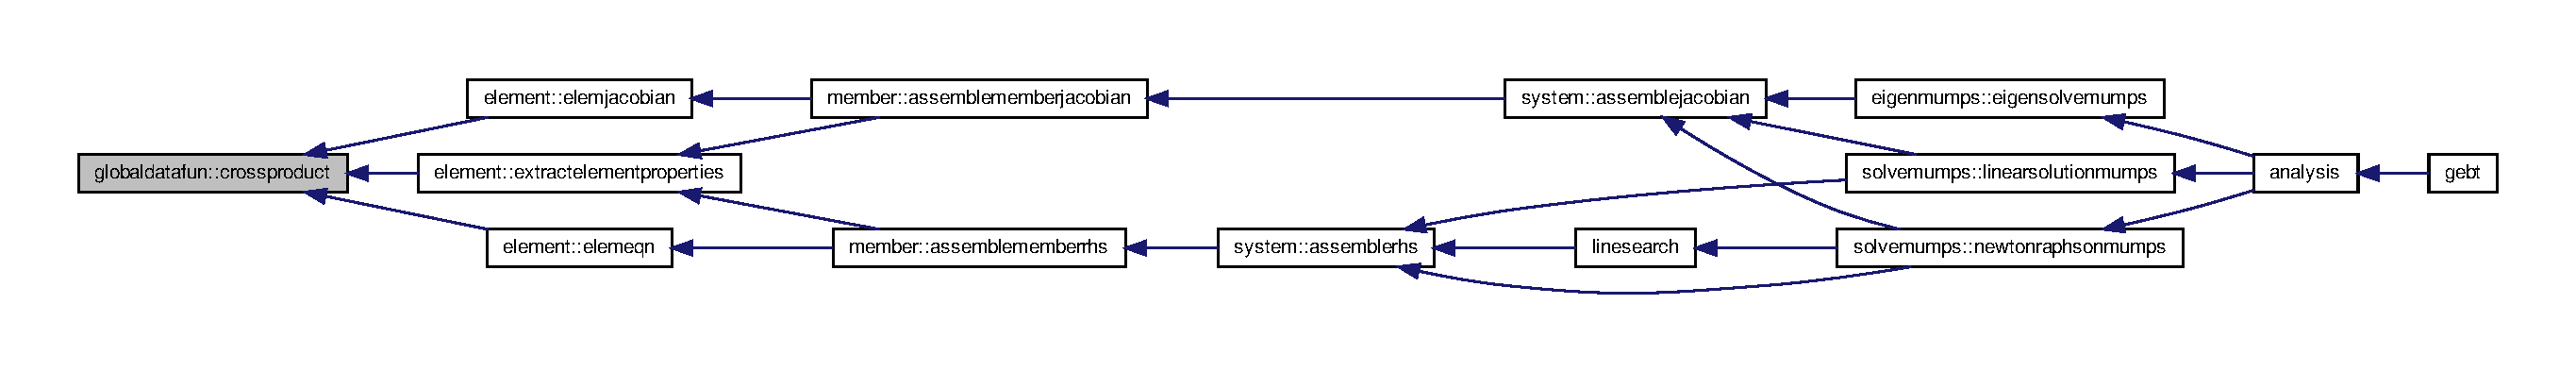
\includegraphics[width=350pt]{namespaceglobaldatafun_a5b4feec69bb3f3464bcd8c08406f9c82_icgraph}
\end{center}
\end{figure}
\mbox{\Hypertarget{namespaceglobaldatafun_a166b3774feeda05d1e3d1761c1412e85}\label{namespaceglobaldatafun_a166b3774feeda05d1e3d1761c1412e85}} 
\index{globaldatafun@{globaldatafun}!ct\+\_\+theta@{ct\+\_\+theta}}
\index{ct\+\_\+theta@{ct\+\_\+theta}!globaldatafun@{globaldatafun}}
\subsubsection{\texorpdfstring{ct\+\_\+theta()}{ct\_theta()}}
{\footnotesize\ttfamily subroutine, public globaldatafun\+::ct\+\_\+theta (\begin{DoxyParamCaption}\item[{real(\hyperlink{namespaceglobaldatafun_a5008801201dd34f2af8eae07756befb4}{dbl}), dimension(\+:), intent(in)}]{theta,  }\item[{real(\hyperlink{namespaceglobaldatafun_a5008801201dd34f2af8eae07756befb4}{dbl}), dimension(\+:,\+:), intent(in)}]{e\+CT,  }\item[{real(\hyperlink{namespaceglobaldatafun_a5008801201dd34f2af8eae07756befb4}{dbl}), dimension(\+:,\+:,\+:), intent(out)}]{ekttek,  }\item[{real(\hyperlink{namespaceglobaldatafun_a5008801201dd34f2af8eae07756befb4}{dbl}), dimension(\+:,\+:,\+:), intent(out)}]{e\+C\+Ttheta }\end{DoxyParamCaption})}



Calculate e\+C$^\wedge$T derivative w.\+r.\+t theta $\ast$ return derivative and ekttek $\ast$. 


\begin{DoxyParams}[1]{Parameters}
\mbox{\tt in}  & {\em theta} & Rodrigues rotation parameters\\
\hline
\mbox{\tt in}  & {\em ect} & Direction Cosine matrix between frame b and B\\
\hline
\mbox{\tt out}  & {\em ekttek} & =Outer\+Product(ek,theta)+\+Outer\+Product(theta,ek)\\
\hline
\mbox{\tt out}  & {\em ecttheta} & Derivatives of e\+CT relative to theta \\
\hline
\end{DoxyParams}


Definition at line 426 of file Global\+Data\+Fun.\+f90.

Here is the caller graph for this function\+:\nopagebreak
\begin{figure}[H]
\begin{center}
\leavevmode
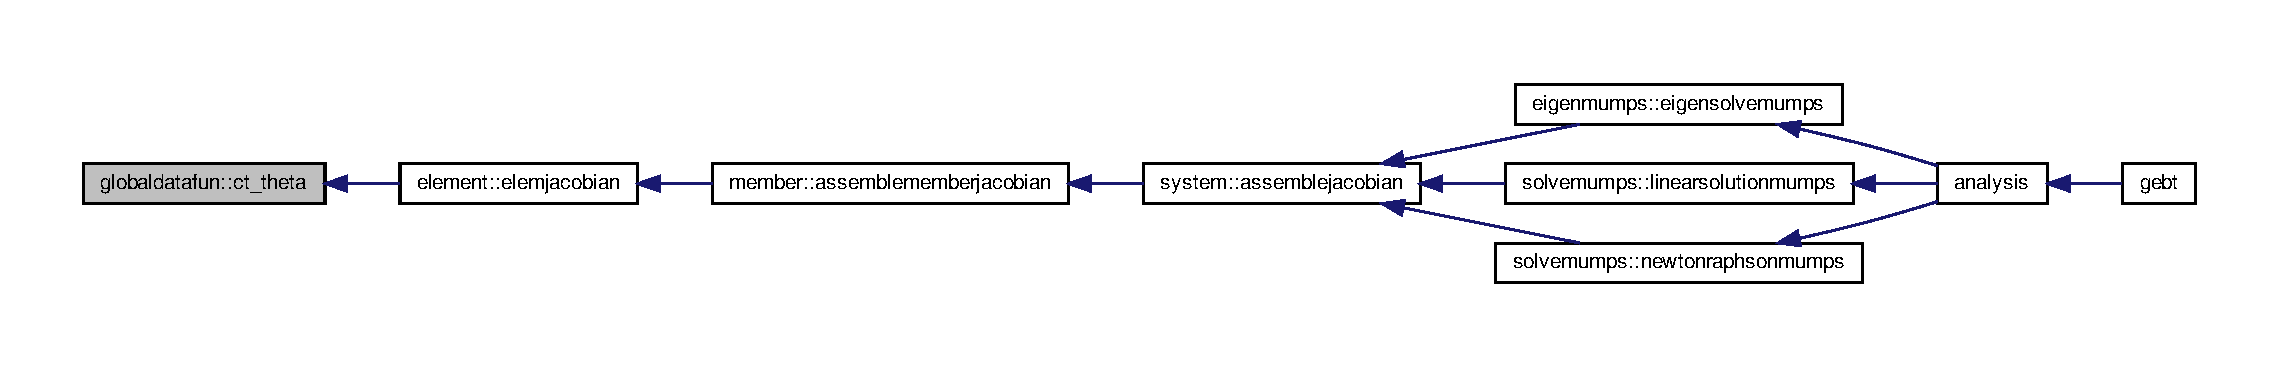
\includegraphics[width=350pt]{namespaceglobaldatafun_a166b3774feeda05d1e3d1761c1412e85_icgraph}
\end{center}
\end{figure}
\mbox{\Hypertarget{namespaceglobaldatafun_a88e61f954347d95bbbbeb6b4aa6f2e8f}\label{namespaceglobaldatafun_a88e61f954347d95bbbbeb6b4aa6f2e8f}} 
\index{globaldatafun@{globaldatafun}!ct\+\_\+theta\+\_\+t@{ct\+\_\+theta\+\_\+t}}
\index{ct\+\_\+theta\+\_\+t@{ct\+\_\+theta\+\_\+t}!globaldatafun@{globaldatafun}}
\subsubsection{\texorpdfstring{ct\+\_\+theta\+\_\+t()}{ct\_theta\_t()}}
{\footnotesize\ttfamily real(\hyperlink{namespaceglobaldatafun_a5008801201dd34f2af8eae07756befb4}{dbl}) function, dimension(3,3), public globaldatafun\+::ct\+\_\+theta\+\_\+t (\begin{DoxyParamCaption}\item[{real(\hyperlink{namespaceglobaldatafun_a5008801201dd34f2af8eae07756befb4}{dbl}), dimension(\+:), intent(in)}]{theta,  }\item[{real(\hyperlink{namespaceglobaldatafun_a5008801201dd34f2af8eae07756befb4}{dbl}), dimension(\+:,\+:), intent(in)}]{e\+CT,  }\item[{real(\hyperlink{namespaceglobaldatafun_a5008801201dd34f2af8eae07756befb4}{dbl}), dimension(\+:), intent(in)}]{x }\end{DoxyParamCaption})}



Calculate $ \dot{eC^T}.x $ derivative w.\+r.\+t $ \dot{theta} $ $\ast$. 


\begin{DoxyParams}[1]{Parameters}
\mbox{\tt in}  & {\em theta} & Rodrigues rotation parameters\\
\hline
\mbox{\tt in}  & {\em ect} & Direction Cosine matrix between frame b and B\\
\hline
\mbox{\tt in}  & {\em x} & vector \\
\hline
\end{DoxyParams}


Definition at line 453 of file Global\+Data\+Fun.\+f90.

Here is the caller graph for this function\+:\nopagebreak
\begin{figure}[H]
\begin{center}
\leavevmode
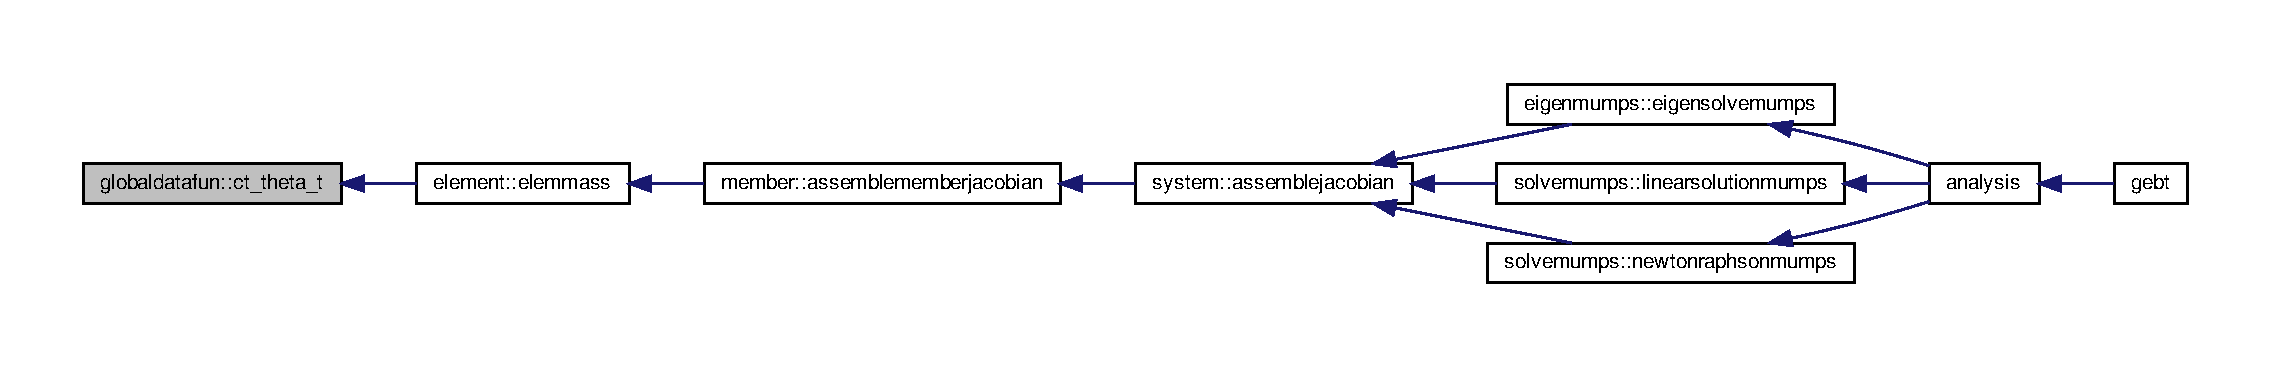
\includegraphics[width=350pt]{namespaceglobaldatafun_a88e61f954347d95bbbbeb6b4aa6f2e8f_icgraph}
\end{center}
\end{figure}
\mbox{\Hypertarget{namespaceglobaldatafun_a79e0439ba9c19e8c9bd28d76417cc4db}\label{namespaceglobaldatafun_a79e0439ba9c19e8c9bd28d76417cc4db}} 
\index{globaldatafun@{globaldatafun}!dircosinetrodrigues@{dircosinetrodrigues}}
\index{dircosinetrodrigues@{dircosinetrodrigues}!globaldatafun@{globaldatafun}}
\subsubsection{\texorpdfstring{dircosinetrodrigues()}{dircosinetrodrigues()}}
{\footnotesize\ttfamily real(\hyperlink{namespaceglobaldatafun_a5008801201dd34f2af8eae07756befb4}{dbl}) function, dimension(3,3), public globaldatafun\+::dircosinetrodrigues (\begin{DoxyParamCaption}\item[{real(\hyperlink{namespaceglobaldatafun_a5008801201dd34f2af8eae07756befb4}{dbl}), dimension(\+:), intent(in)}]{theta }\end{DoxyParamCaption})}



Calculate the transpose of the direction cosine in $\ast$ terms of rodrigues parameters $\ast$. 



Definition at line 479 of file Global\+Data\+Fun.\+f90.

Here is the caller graph for this function\+:\nopagebreak
\begin{figure}[H]
\begin{center}
\leavevmode
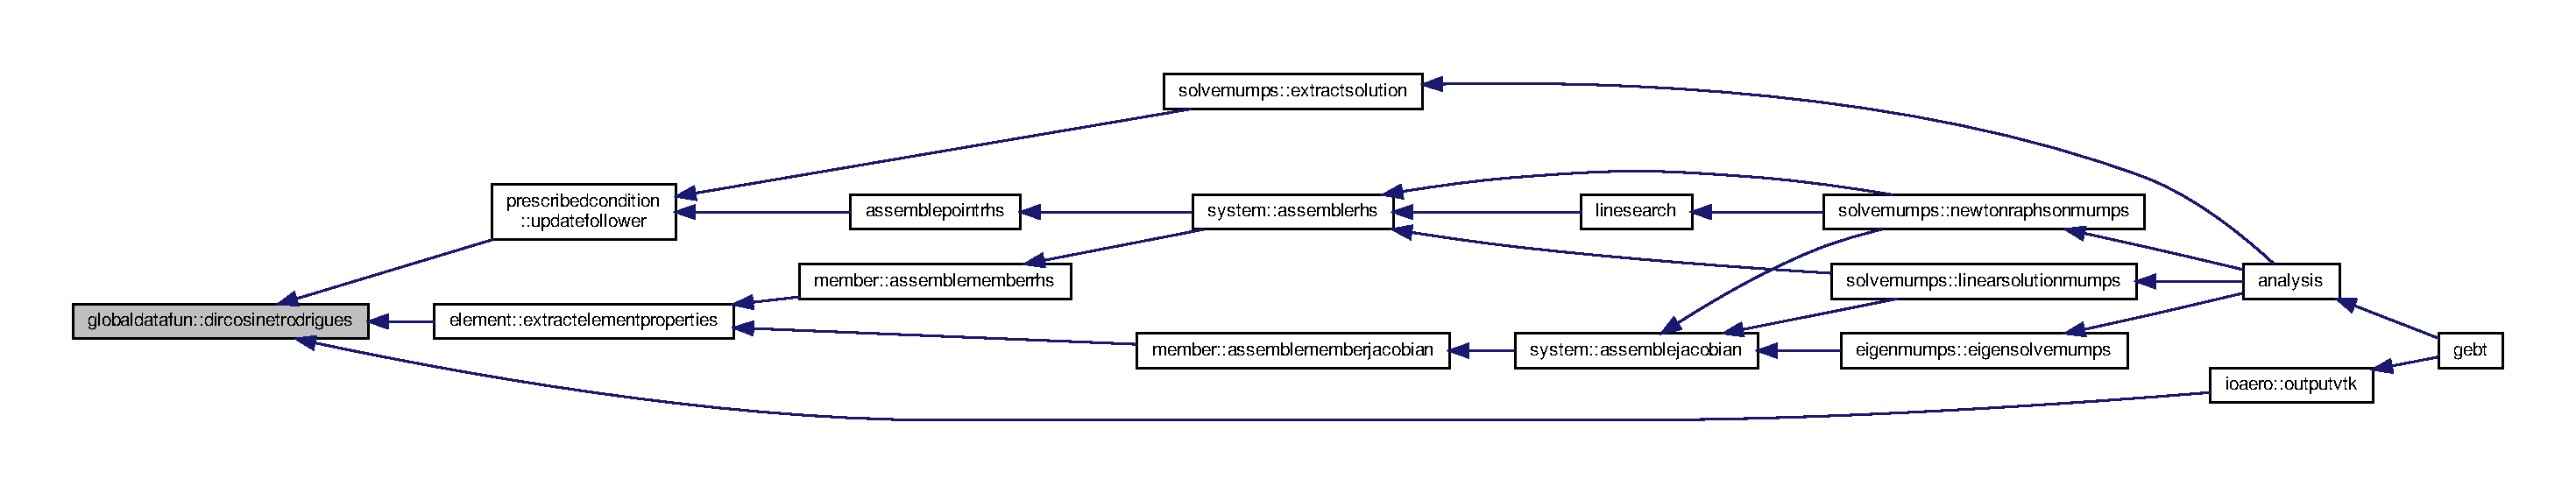
\includegraphics[width=350pt]{namespaceglobaldatafun_a79e0439ba9c19e8c9bd28d76417cc4db_icgraph}
\end{center}
\end{figure}
\mbox{\Hypertarget{namespaceglobaldatafun_a8068755a2ac0857cf1dfc681e43af3a8}\label{namespaceglobaldatafun_a8068755a2ac0857cf1dfc681e43af3a8}} 
\index{globaldatafun@{globaldatafun}!extract2delement@{extract2delement}}
\index{extract2delement@{extract2delement}!globaldatafun@{globaldatafun}}
\subsubsection{\texorpdfstring{extract2delement()}{extract2delement()}}
{\footnotesize\ttfamily subroutine, public globaldatafun\+::extract2delement (\begin{DoxyParamCaption}\item[{integer, intent(in)}]{nz,  }\item[{integer, dimension(\+:), intent(in)}]{irn,  }\item[{integer, dimension(\+:), intent(in)}]{jcn,  }\item[{real(\hyperlink{namespaceglobaldatafun_a5008801201dd34f2af8eae07756befb4}{dbl}), dimension(\+:), intent(in)}]{elem\+Coef1D,  }\item[{real(\hyperlink{namespaceglobaldatafun_a5008801201dd34f2af8eae07756befb4}{dbl}), dimension(\+:,\+:), intent(out)}]{tmpR,  }\item[{integer, intent(in)}]{str\+\_\+r1,  }\item[{integer, intent(in)}]{str\+\_\+c1 }\end{DoxyParamCaption})}



Back a 2D array from the 1D coefficient matrix. 



Definition at line 725 of file Global\+Data\+Fun.\+f90.

\mbox{\Hypertarget{namespaceglobaldatafun_a0ae214f4b91d5705b4d0107913efe369}\label{namespaceglobaldatafun_a0ae214f4b91d5705b4d0107913efe369}} 
\index{globaldatafun@{globaldatafun}!factoriel@{factoriel}}
\index{factoriel@{factoriel}!globaldatafun@{globaldatafun}}
\subsubsection{\texorpdfstring{factoriel()}{factoriel()}}
{\footnotesize\ttfamily real(\hyperlink{namespaceglobaldatafun_a5008801201dd34f2af8eae07756befb4}{dbl}) function globaldatafun\+::factoriel (\begin{DoxyParamCaption}\item[{integer, intent(in)}]{n }\end{DoxyParamCaption})\hspace{0.3cm}{\ttfamily [private]}}



Compute the value of factoriel(n) 



Definition at line 891 of file Global\+Data\+Fun.\+f90.

Here is the caller graph for this function\+:\nopagebreak
\begin{figure}[H]
\begin{center}
\leavevmode
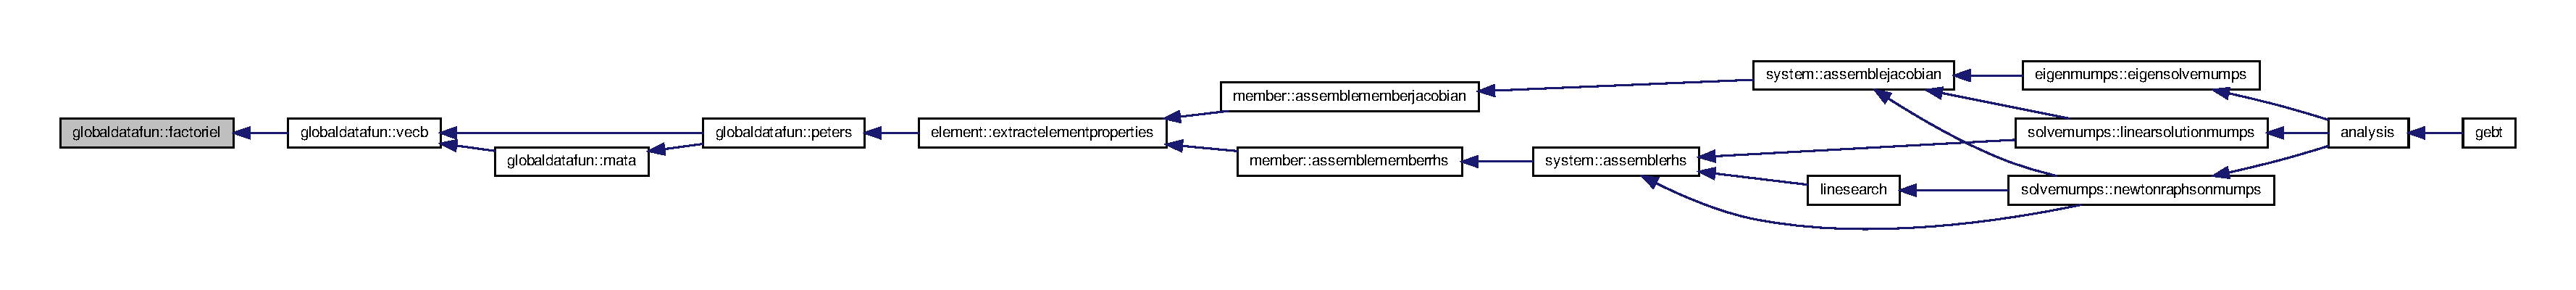
\includegraphics[width=350pt]{namespaceglobaldatafun_a0ae214f4b91d5705b4d0107913efe369_icgraph}
\end{center}
\end{figure}
\mbox{\Hypertarget{namespaceglobaldatafun_a384e8e6270f765a8e68a8c65ac8ae9d6}\label{namespaceglobaldatafun_a384e8e6270f765a8e68a8c65ac8ae9d6}} 
\index{globaldatafun@{globaldatafun}!fileopen@{fileopen}}
\index{fileopen@{fileopen}!globaldatafun@{globaldatafun}}
\subsubsection{\texorpdfstring{fileopen()}{fileopen()}}
{\footnotesize\ttfamily logical function, public globaldatafun\+::fileopen (\begin{DoxyParamCaption}\item[{integer, intent(in)}]{file\+\_\+unit,  }\item[{character($\ast$), intent(in)}]{file\+\_\+name,  }\item[{character($\ast$), intent(in)}]{sta\+\_\+type,  }\item[{character($\ast$), intent(in)}]{rw\+\_\+type,  }\item[{character($\ast$), intent(out)}]{error }\end{DoxyParamCaption})}



To open an old or new file for reading or writing $\ast$. 


\begin{DoxyParams}[1]{Parameters}
\mbox{\tt in}  & {\em file\+\_\+unit} & File Unit (see fortran IO doc)\\
\hline
\mbox{\tt in}  & {\em sta\+\_\+type} & status type\\
\hline
\mbox{\tt in}  & {\em rw\+\_\+type} & rewrite configuration\\
\hline
\mbox{\tt out}  & {\em error} & \hyperlink{namespaceioaero_aebd85ae2a176f49a7213d8ed7b68f887}{ioaero\+::error} \\
\hline
\end{DoxyParams}


Definition at line 167 of file Global\+Data\+Fun.\+f90.

Here is the caller graph for this function\+:\nopagebreak
\begin{figure}[H]
\begin{center}
\leavevmode
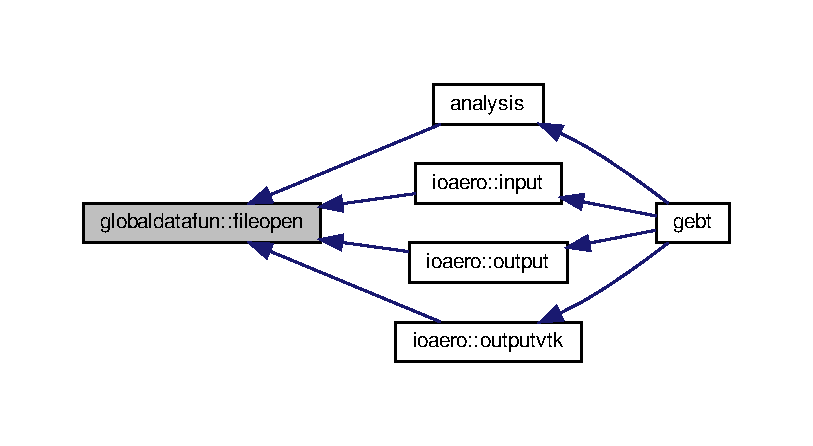
\includegraphics[width=350pt]{namespaceglobaldatafun_a384e8e6270f765a8e68a8c65ac8ae9d6_icgraph}
\end{center}
\end{figure}
\mbox{\Hypertarget{namespaceglobaldatafun_a8ea8d9cf6c54128f3e5df19d4d0170da}\label{namespaceglobaldatafun_a8ea8d9cf6c54128f3e5df19d4d0170da}} 
\index{globaldatafun@{globaldatafun}!insert1delement@{insert1delement}}
\index{insert1delement@{insert1delement}!globaldatafun@{globaldatafun}}
\subsubsection{\texorpdfstring{insert1delement()}{insert1delement()}}
{\footnotesize\ttfamily subroutine, public globaldatafun\+::insert1delement (\begin{DoxyParamCaption}\item[{integer, intent(inout)}]{nz,  }\item[{real(\hyperlink{namespaceglobaldatafun_a5008801201dd34f2af8eae07756befb4}{dbl}), dimension(\+:,\+:), intent(in)}]{tmpR,  }\item[{integer, dimension(\+:), intent(inout)}]{irn,  }\item[{integer, dimension(\+:), intent(inout)}]{jcn,  }\item[{real(\hyperlink{namespaceglobaldatafun_a5008801201dd34f2af8eae07756befb4}{dbl}), dimension(\+:), intent(inout)}]{elem\+Coef1D,  }\item[{integer, intent(in)}]{str\+\_\+r1,  }\item[{integer, intent(in)}]{str\+\_\+c1,  }\item[{integer, intent(in), optional}]{str\+\_\+r2,  }\item[{integer, intent(in), optional}]{str\+\_\+c2,  }\item[{integer, intent(in), optional}]{str\+\_\+r3,  }\item[{integer, intent(in), optional}]{str\+\_\+c3,  }\item[{integer, intent(in), optional}]{str\+\_\+r4,  }\item[{integer, intent(in), optional}]{str\+\_\+c4 }\end{DoxyParamCaption})}



Insert a real matrix into the 1D coefficient matrix. 



Definition at line 671 of file Global\+Data\+Fun.\+f90.

\mbox{\Hypertarget{namespaceglobaldatafun_a1e393f2df119550fc86d1c0864fde446}\label{namespaceglobaldatafun_a1e393f2df119550fc86d1c0864fde446}} 
\index{globaldatafun@{globaldatafun}!invert@{invert}}
\index{invert@{invert}!globaldatafun@{globaldatafun}}
\subsubsection{\texorpdfstring{invert()}{invert()}}
{\footnotesize\ttfamily subroutine, public globaldatafun\+::invert (\begin{DoxyParamCaption}\item[{real(\hyperlink{namespaceglobaldatafun_a5008801201dd34f2af8eae07756befb4}{dbl}), dimension(\+:,\+:), intent(in)}]{matrix\+\_\+in,  }\item[{real(\hyperlink{namespaceglobaldatafun_a5008801201dd34f2af8eae07756befb4}{dbl}), dimension(\+:,\+:), intent(out)}]{matrix,  }\item[{character($\ast$), intent(in)}]{vari\+\_\+name,  }\item[{character($\ast$), intent(out)}]{error }\end{DoxyParamCaption})}



Invert a small square matrix $\ast$. 


\begin{DoxyParams}[1]{Parameters}
\mbox{\tt in}  & {\em matrix\+\_\+in} & the matrix to be inverted\\
\hline
\mbox{\tt out}  & {\em matrix} & the inverse of the matrix \\
\hline
\end{DoxyParams}


Definition at line 498 of file Global\+Data\+Fun.\+f90.

\mbox{\Hypertarget{namespaceglobaldatafun_a84403b06e98cfc25fc1fb6222884a30d}\label{namespaceglobaldatafun_a84403b06e98cfc25fc1fb6222884a30d}} 
\index{globaldatafun@{globaldatafun}!ioerror@{ioerror}}
\index{ioerror@{ioerror}!globaldatafun@{globaldatafun}}
\subsubsection{\texorpdfstring{ioerror()}{ioerror()}}
{\footnotesize\ttfamily logical function, public globaldatafun\+::ioerror (\begin{DoxyParamCaption}\item[{character($\ast$), intent(in)}]{message,  }\item[{character($\ast$), intent(out)}]{error }\end{DoxyParamCaption})}



Check the error of I/O processing $\ast$. 


\begin{DoxyParams}[1]{Parameters}
\mbox{\tt in}  & {\em message} & a character variable to hold error message\\
\hline
\mbox{\tt out}  & {\em error} & \hyperlink{namespaceioaero_aebd85ae2a176f49a7213d8ed7b68f887}{ioaero\+::error} \\
\hline
\end{DoxyParams}


Definition at line 198 of file Global\+Data\+Fun.\+f90.

Here is the caller graph for this function\+:\nopagebreak
\begin{figure}[H]
\begin{center}
\leavevmode
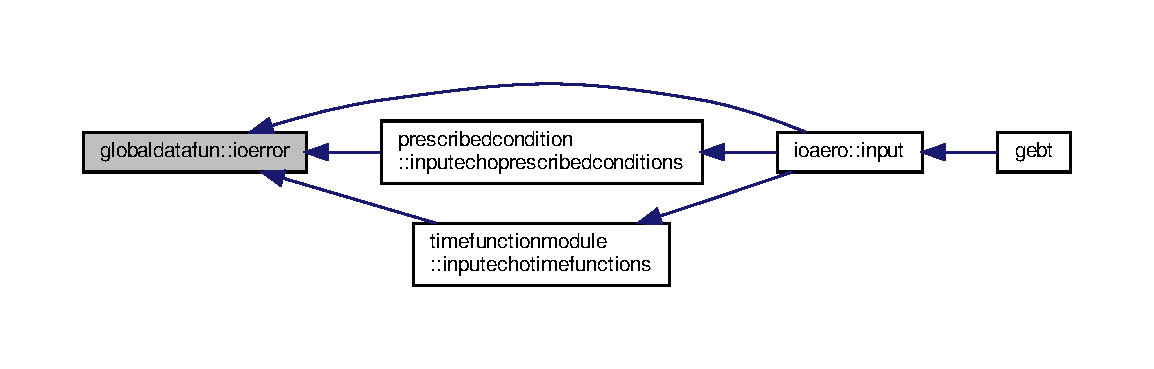
\includegraphics[width=350pt]{namespaceglobaldatafun_a84403b06e98cfc25fc1fb6222884a30d_icgraph}
\end{center}
\end{figure}
\mbox{\Hypertarget{namespaceglobaldatafun_ae970761ddf59b4acff02030b21dbcd75}\label{namespaceglobaldatafun_ae970761ddf59b4acff02030b21dbcd75}} 
\index{globaldatafun@{globaldatafun}!itochar@{itochar}}
\index{itochar@{itochar}!globaldatafun@{globaldatafun}}
\subsubsection{\texorpdfstring{itochar()}{itochar()}}
{\footnotesize\ttfamily character(20) function globaldatafun\+::itochar (\begin{DoxyParamCaption}\item[{integer, intent(in)}]{n }\end{DoxyParamCaption})\hspace{0.3cm}{\ttfamily [private]}}



Convert an integer to character $\ast$. 



Definition at line 222 of file Global\+Data\+Fun.\+f90.

Here is the caller graph for this function\+:\nopagebreak
\begin{figure}[H]
\begin{center}
\leavevmode
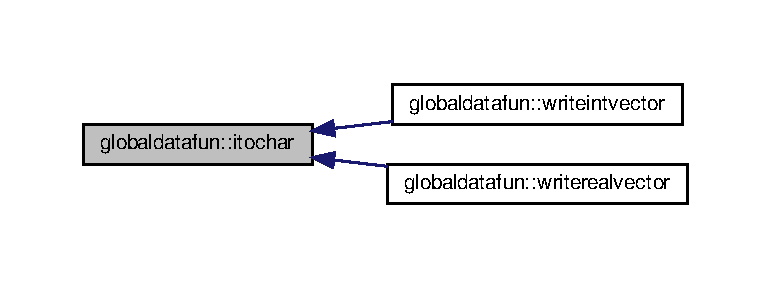
\includegraphics[width=350pt]{namespaceglobaldatafun_ae970761ddf59b4acff02030b21dbcd75_icgraph}
\end{center}
\end{figure}
\mbox{\Hypertarget{namespaceglobaldatafun_abc2a555e679f86fd986da760d49b71bc}\label{namespaceglobaldatafun_abc2a555e679f86fd986da760d49b71bc}} 
\index{globaldatafun@{globaldatafun}!mata@{mata}}
\index{mata@{mata}!globaldatafun@{globaldatafun}}
\subsubsection{\texorpdfstring{mata()}{mata()}}
{\footnotesize\ttfamily real(\hyperlink{namespaceglobaldatafun_a5008801201dd34f2af8eae07756befb4}{dbl}) function, dimension(n,n), public globaldatafun\+::mata (\begin{DoxyParamCaption}\item[{integer, intent(in)}]{n }\end{DoxyParamCaption})}



Compute the Peters A matrix. 



Definition at line 796 of file Global\+Data\+Fun.\+f90.

Here is the caller graph for this function\+:\nopagebreak
\begin{figure}[H]
\begin{center}
\leavevmode
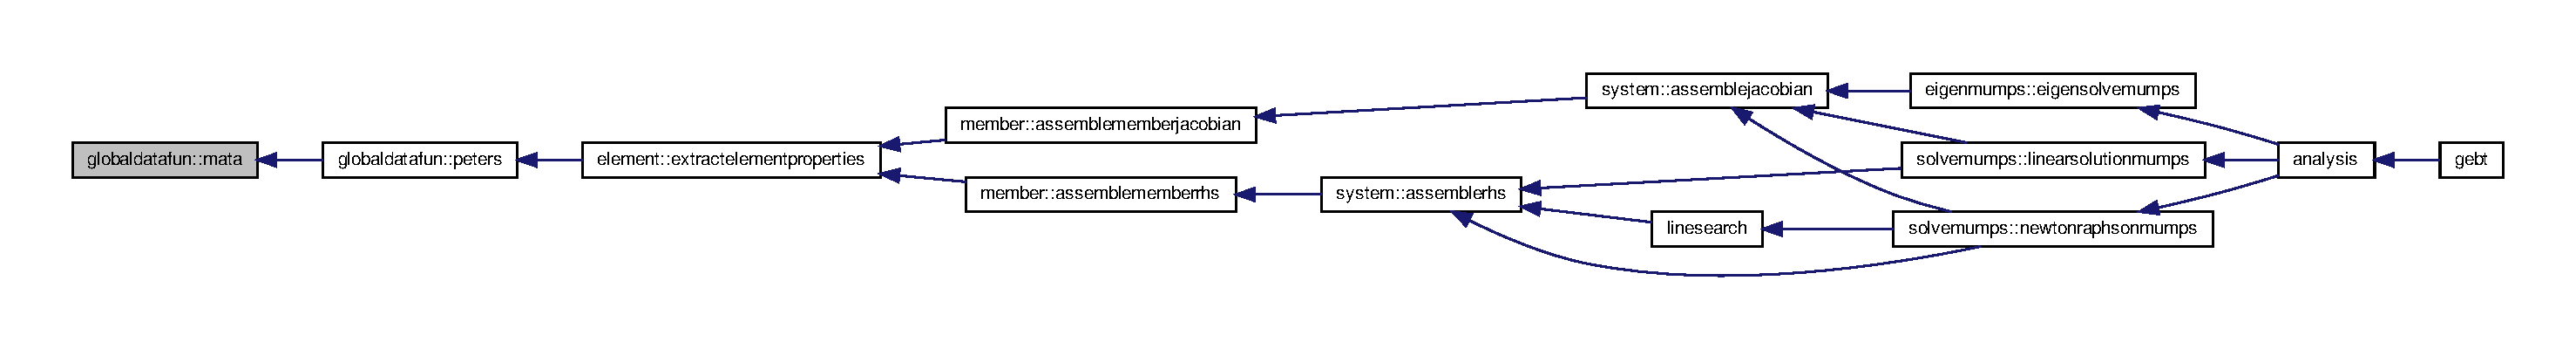
\includegraphics[width=350pt]{namespaceglobaldatafun_abc2a555e679f86fd986da760d49b71bc_icgraph}
\end{center}
\end{figure}
\mbox{\Hypertarget{namespaceglobaldatafun_a5290afbf1d3da671a523a4727bdc7218}\label{namespaceglobaldatafun_a5290afbf1d3da671a523a4727bdc7218}} 
\index{globaldatafun@{globaldatafun}!matd@{matd}}
\index{matd@{matd}!globaldatafun@{globaldatafun}}
\subsubsection{\texorpdfstring{matd()}{matd()}}
{\footnotesize\ttfamily real(\hyperlink{namespaceglobaldatafun_a5008801201dd34f2af8eae07756befb4}{dbl}) function, dimension(n,n) globaldatafun\+::matd (\begin{DoxyParamCaption}\item[{integer, intent(in)}]{n }\end{DoxyParamCaption})\hspace{0.3cm}{\ttfamily [private]}}



Compute the Peters D matrix. 



Definition at line 807 of file Global\+Data\+Fun.\+f90.

Here is the caller graph for this function\+:\nopagebreak
\begin{figure}[H]
\begin{center}
\leavevmode
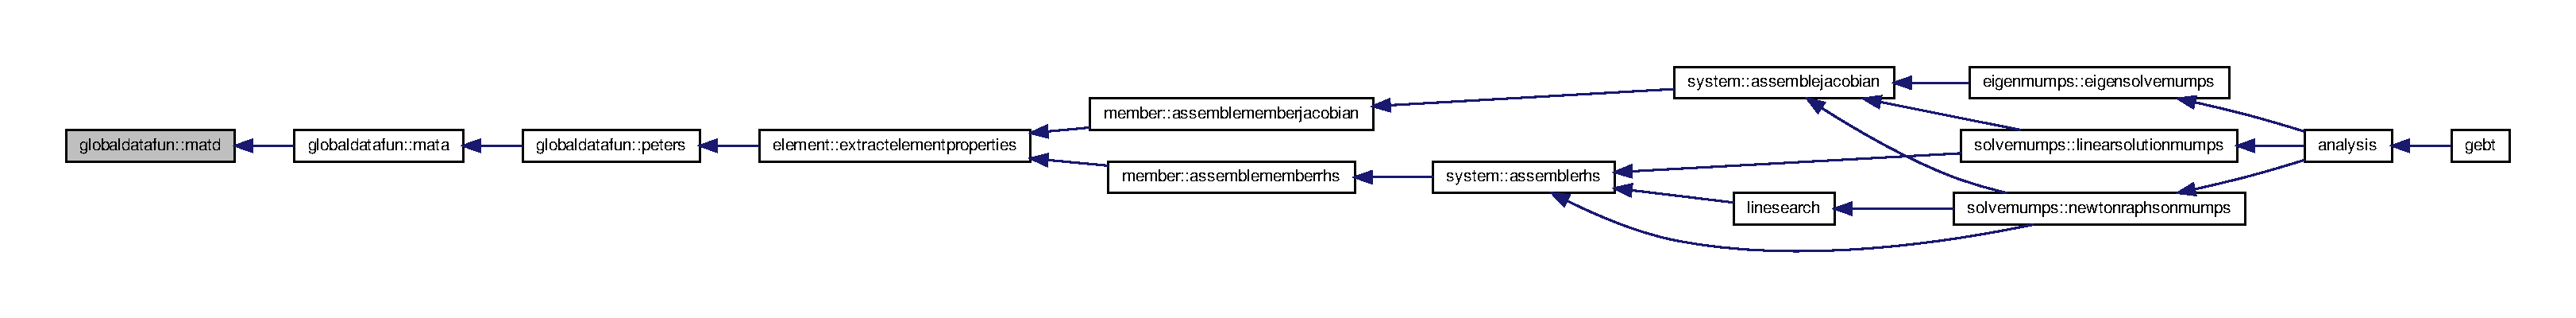
\includegraphics[width=350pt]{namespaceglobaldatafun_a5290afbf1d3da671a523a4727bdc7218_icgraph}
\end{center}
\end{figure}
\mbox{\Hypertarget{namespaceglobaldatafun_a562042b12250dbd7e3ef3a24d9f93a53}\label{namespaceglobaldatafun_a562042b12250dbd7e3ef3a24d9f93a53}} 
\index{globaldatafun@{globaldatafun}!matmul3@{matmul3}}
\index{matmul3@{matmul3}!globaldatafun@{globaldatafun}}
\subsubsection{\texorpdfstring{matmul3()}{matmul3()}}
{\footnotesize\ttfamily real(\hyperlink{namespaceglobaldatafun_a5008801201dd34f2af8eae07756befb4}{dbl}) function, dimension(size(mat,1),size(mat,2)), public globaldatafun\+::matmul3 (\begin{DoxyParamCaption}\item[{real(\hyperlink{namespaceglobaldatafun_a5008801201dd34f2af8eae07756befb4}{dbl}), dimension(\+:,\+:,\+:), intent(in)}]{mat,  }\item[{real(\hyperlink{namespaceglobaldatafun_a5008801201dd34f2af8eae07756befb4}{dbl}), dimension(\+:), intent(in)}]{vec }\end{DoxyParamCaption})}



Multiply a rank 3 matrix with a vector with every colum $\ast$ of the resulting matrix is equal to the multiplication $\ast$. 



Definition at line 554 of file Global\+Data\+Fun.\+f90.

Here is the caller graph for this function\+:\nopagebreak
\begin{figure}[H]
\begin{center}
\leavevmode
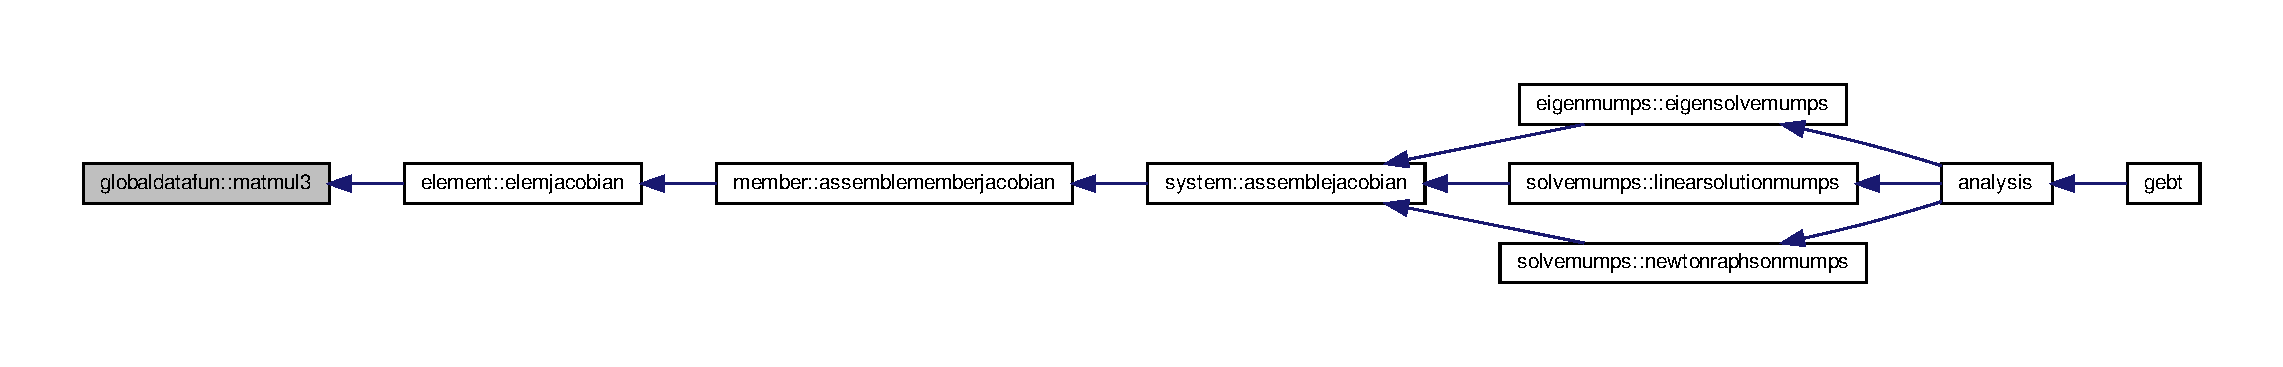
\includegraphics[width=350pt]{namespaceglobaldatafun_a562042b12250dbd7e3ef3a24d9f93a53_icgraph}
\end{center}
\end{figure}
\mbox{\Hypertarget{namespaceglobaldatafun_a370a248c97771d5e9b8410dedbfb548c}\label{namespaceglobaldatafun_a370a248c97771d5e9b8410dedbfb548c}} 
\index{globaldatafun@{globaldatafun}!matmul\+\_\+sparse@{matmul\+\_\+sparse}}
\index{matmul\+\_\+sparse@{matmul\+\_\+sparse}!globaldatafun@{globaldatafun}}
\subsubsection{\texorpdfstring{matmul\+\_\+sparse()}{matmul\_sparse()}}
{\footnotesize\ttfamily real(\hyperlink{namespaceglobaldatafun_a5008801201dd34f2af8eae07756befb4}{dbl}) function, dimension(nsize), public globaldatafun\+::matmul\+\_\+sparse (\begin{DoxyParamCaption}\item[{real(\hyperlink{namespaceglobaldatafun_a5008801201dd34f2af8eae07756befb4}{dbl}), dimension(\+:), intent(in)}]{vector,  }\item[{integer, intent(in)}]{nsize,  }\item[{integer, intent(in)}]{ne,  }\item[{integer, dimension(\+:), intent(in)}]{irn,  }\item[{integer, dimension(\+:), intent(in)}]{jcn,  }\item[{real(\hyperlink{namespaceglobaldatafun_a5008801201dd34f2af8eae07756befb4}{dbl}), dimension(\+:), intent(in)}]{matrix1D }\end{DoxyParamCaption})}



Matmul(vector, matrix) with matrix stored in a spare format. 



Definition at line 758 of file Global\+Data\+Fun.\+f90.

\mbox{\Hypertarget{namespaceglobaldatafun_af28c2b9df0d5a1ef886c3d242fc15205}\label{namespaceglobaldatafun_af28c2b9df0d5a1ef886c3d242fc15205}} 
\index{globaldatafun@{globaldatafun}!memoryerror@{memoryerror}}
\index{memoryerror@{memoryerror}!globaldatafun@{globaldatafun}}
\subsubsection{\texorpdfstring{memoryerror()}{memoryerror()}}
{\footnotesize\ttfamily logical function, public globaldatafun\+::memoryerror (\begin{DoxyParamCaption}\item[{character($\ast$), intent(in)}]{vari\+\_\+name,  }\item[{character($\ast$), intent(out)}]{error }\end{DoxyParamCaption})}



Check the error of memory allocation $\ast$. 


\begin{DoxyParams}[1]{Parameters}
\mbox{\tt in}  & {\em vari\+\_\+name} & a character variable to hold variable name\\
\hline
\mbox{\tt out}  & {\em error} & \hyperlink{namespaceioaero_aebd85ae2a176f49a7213d8ed7b68f887}{ioaero\+::error} \\
\hline
\end{DoxyParams}


Definition at line 267 of file Global\+Data\+Fun.\+f90.

Here is the caller graph for this function\+:\nopagebreak
\begin{figure}[H]
\begin{center}
\leavevmode
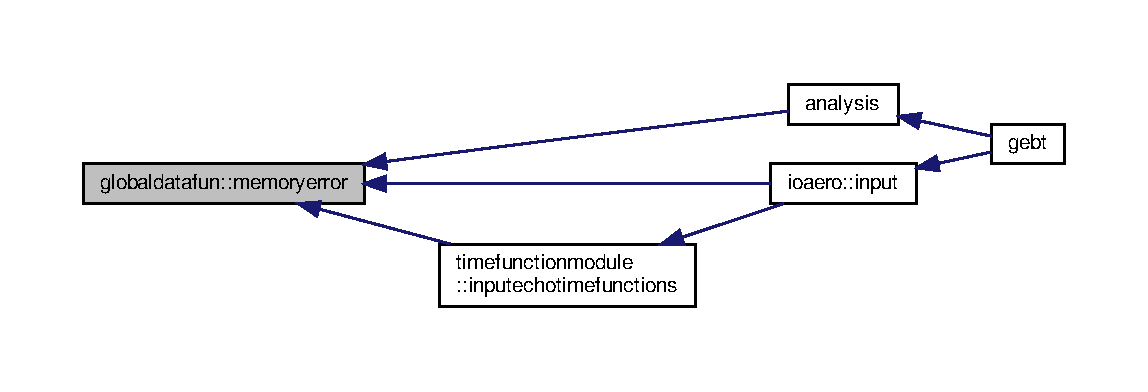
\includegraphics[width=350pt]{namespaceglobaldatafun_af28c2b9df0d5a1ef886c3d242fc15205_icgraph}
\end{center}
\end{figure}
\mbox{\Hypertarget{namespaceglobaldatafun_a79010ea3a4434936e8a71182e62b6e48}\label{namespaceglobaldatafun_a79010ea3a4434936e8a71182e62b6e48}} 
\index{globaldatafun@{globaldatafun}!norm@{norm}}
\index{norm@{norm}!globaldatafun@{globaldatafun}}
\subsubsection{\texorpdfstring{norm()}{norm()}}
{\footnotesize\ttfamily real(\hyperlink{namespaceglobaldatafun_a5008801201dd34f2af8eae07756befb4}{dbl}) function, public globaldatafun\+::norm (\begin{DoxyParamCaption}\item[{real(\hyperlink{namespaceglobaldatafun_a5008801201dd34f2af8eae07756befb4}{dbl}), dimension(\+:), intent(in)}]{vector }\end{DoxyParamCaption})}



Calculate the L2 norm of a real vector $\ast$. 



Definition at line 578 of file Global\+Data\+Fun.\+f90.

Here is the caller graph for this function\+:\nopagebreak
\begin{figure}[H]
\begin{center}
\leavevmode
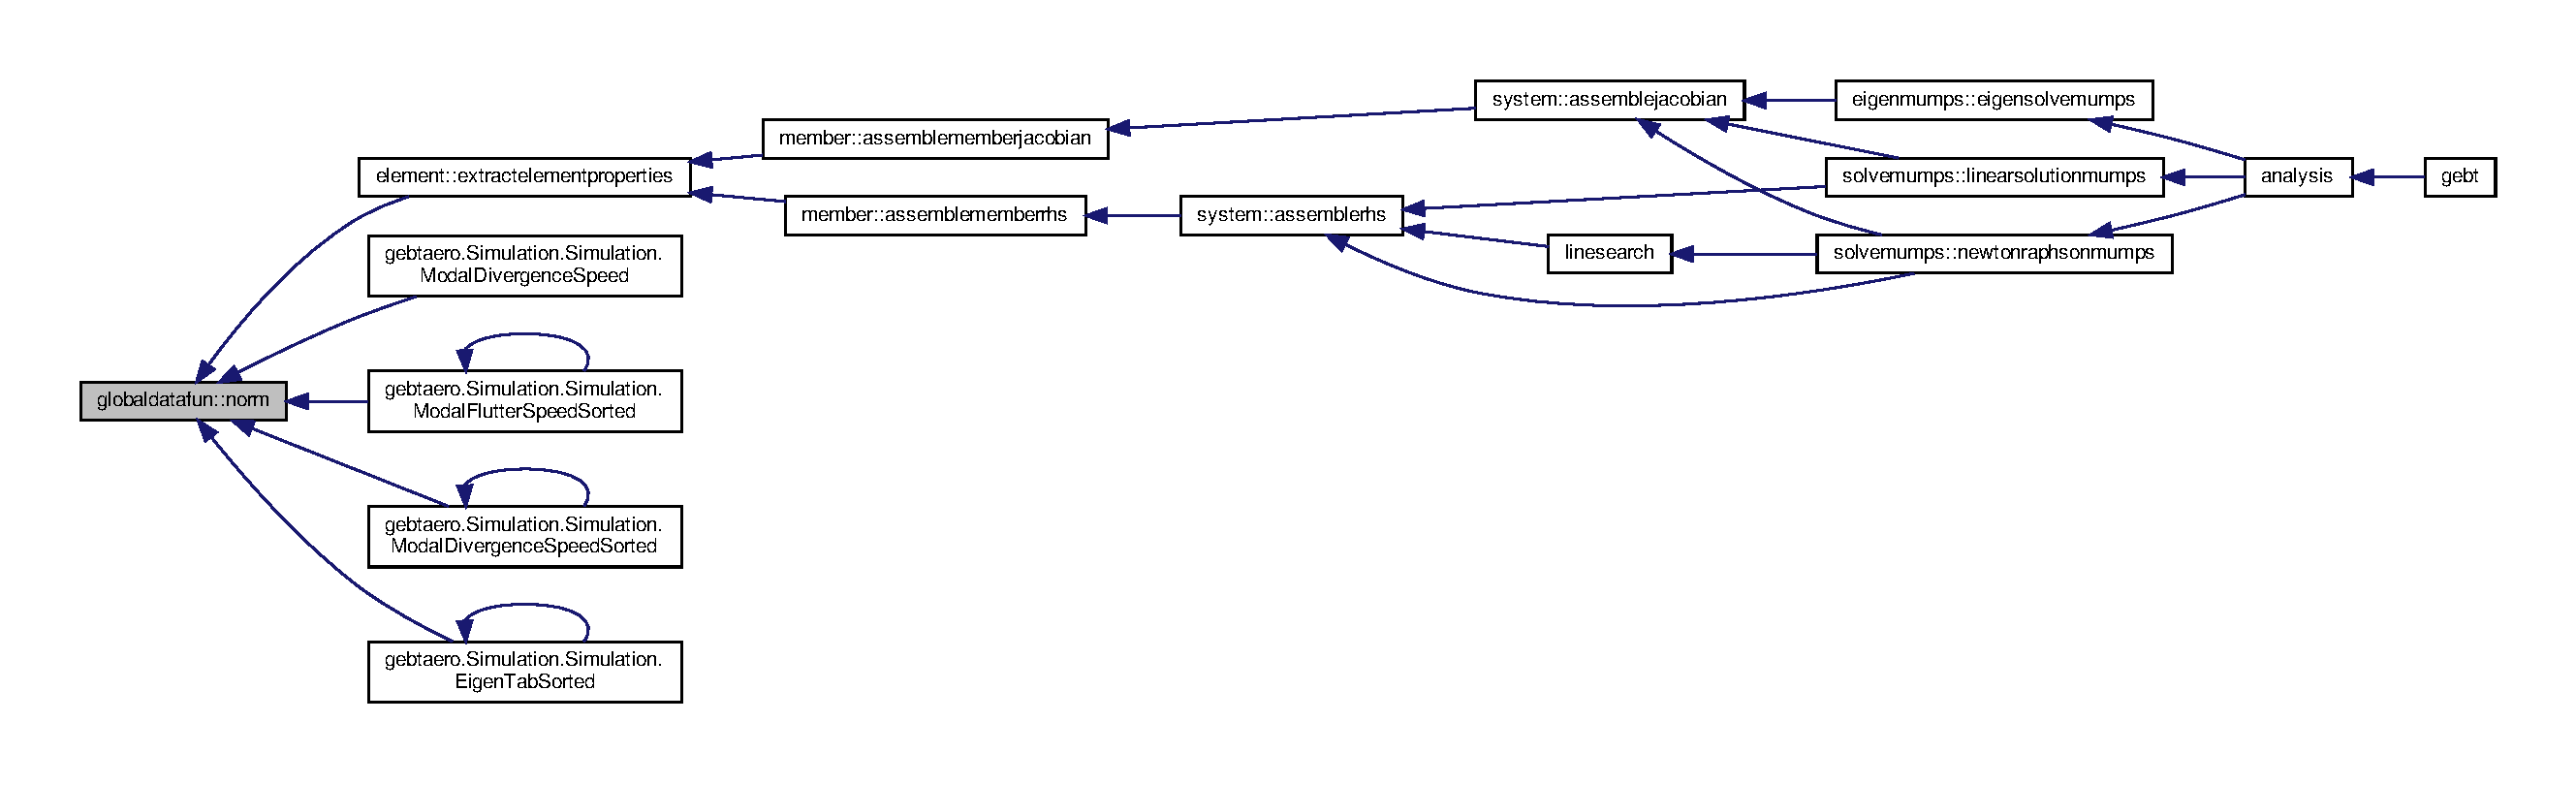
\includegraphics[width=350pt]{namespaceglobaldatafun_a79010ea3a4434936e8a71182e62b6e48_icgraph}
\end{center}
\end{figure}
\mbox{\Hypertarget{namespaceglobaldatafun_af49b8ee04a8cfd5d42b863a092e17e91}\label{namespaceglobaldatafun_af49b8ee04a8cfd5d42b863a092e17e91}} 
\index{globaldatafun@{globaldatafun}!outerproduct@{outerproduct}}
\index{outerproduct@{outerproduct}!globaldatafun@{globaldatafun}}
\subsubsection{\texorpdfstring{outerproduct()}{outerproduct()}}
{\footnotesize\ttfamily real(\hyperlink{namespaceglobaldatafun_a5008801201dd34f2af8eae07756befb4}{dbl}) function, dimension(size(vec1),size(vec2)), public globaldatafun\+::outerproduct (\begin{DoxyParamCaption}\item[{real(\hyperlink{namespaceglobaldatafun_a5008801201dd34f2af8eae07756befb4}{dbl}), dimension(\+:), intent(in)}]{vec1,  }\item[{real(\hyperlink{namespaceglobaldatafun_a5008801201dd34f2af8eae07756befb4}{dbl}), dimension(\+:), intent(in)}]{vec2 }\end{DoxyParamCaption})}



Calculate the outer product of two vectors $\ast$. 



Definition at line 595 of file Global\+Data\+Fun.\+f90.

Here is the caller graph for this function\+:\nopagebreak
\begin{figure}[H]
\begin{center}
\leavevmode
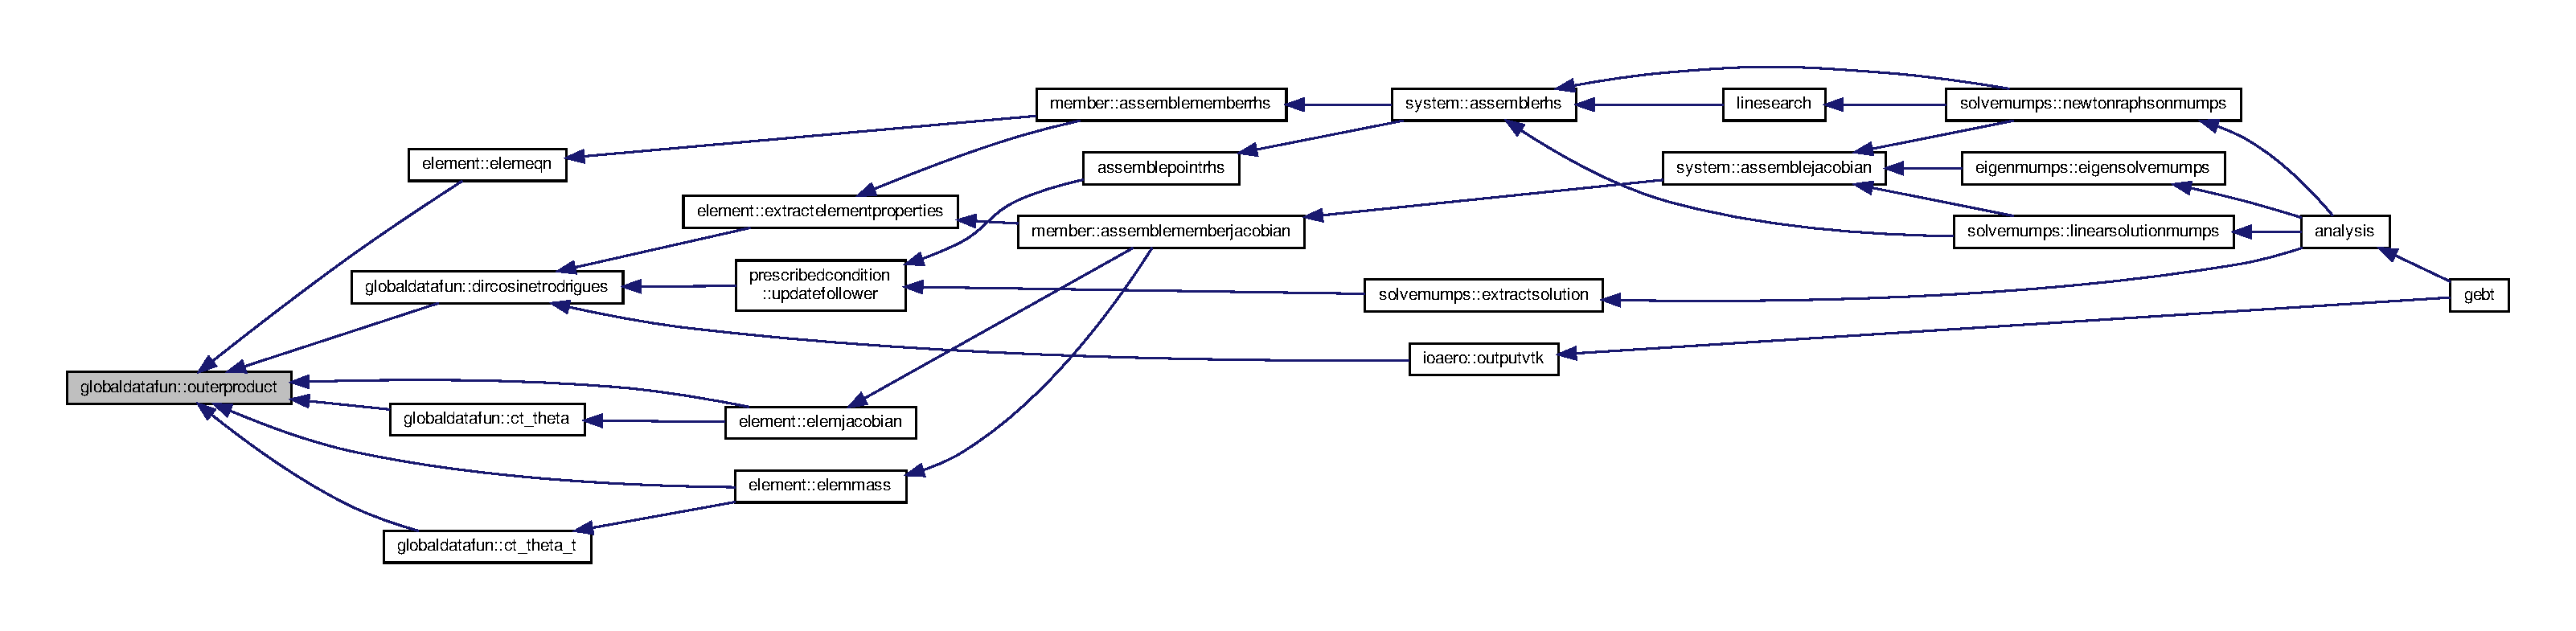
\includegraphics[width=350pt]{namespaceglobaldatafun_af49b8ee04a8cfd5d42b863a092e17e91_icgraph}
\end{center}
\end{figure}
\mbox{\Hypertarget{namespaceglobaldatafun_a9bdeebcd65cb298adc440430560beddc}\label{namespaceglobaldatafun_a9bdeebcd65cb298adc440430560beddc}} 
\index{globaldatafun@{globaldatafun}!peters@{peters}}
\index{peters@{peters}!globaldatafun@{globaldatafun}}
\subsubsection{\texorpdfstring{peters()}{peters()}}
{\footnotesize\ttfamily real(\hyperlink{namespaceglobaldatafun_a5008801201dd34f2af8eae07756befb4}{dbl}) function, dimension(n,2$\ast$n+2), public globaldatafun\+::peters (\begin{DoxyParamCaption}\item[{integer, intent(in)}]{n }\end{DoxyParamCaption})}



Functions used for the Finite State Unsteady Thin Airfoil Theory of Peters see Introduction to Structural Dynamics and Aeroelasticity by Hodges p 139. 


\begin{DoxyParams}[1]{Parameters}
\mbox{\tt in}  & {\em n} & Number of induced flow states (Ns)\\
\hline
\end{DoxyParams}
\begin{DoxyReturn}{Returns}
Matrix containing ordered in line \+: the A matrix, the B vector the C vector, the Identity matrix 
\end{DoxyReturn}


Definition at line 780 of file Global\+Data\+Fun.\+f90.

Here is the caller graph for this function\+:\nopagebreak
\begin{figure}[H]
\begin{center}
\leavevmode
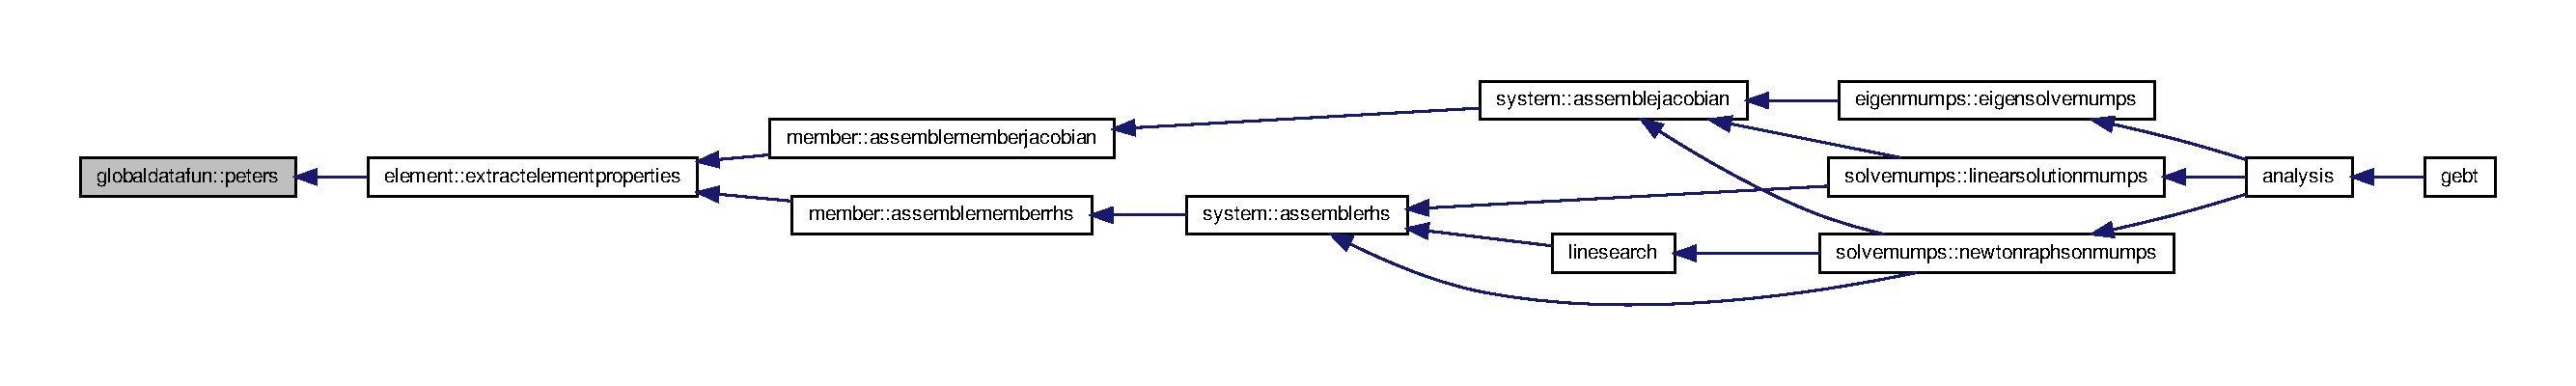
\includegraphics[width=350pt]{namespaceglobaldatafun_a9bdeebcd65cb298adc440430560beddc_icgraph}
\end{center}
\end{figure}
\mbox{\Hypertarget{namespaceglobaldatafun_afe68f9e5d61e5e7844a0a4b225bb3825}\label{namespaceglobaldatafun_afe68f9e5d61e5e7844a0a4b225bb3825}} 
\index{globaldatafun@{globaldatafun}!prod@{prod}}
\index{prod@{prod}!globaldatafun@{globaldatafun}}
\subsubsection{\texorpdfstring{prod()}{prod()}}
{\footnotesize\ttfamily real(\hyperlink{namespaceglobaldatafun_a5008801201dd34f2af8eae07756befb4}{dbl}) function, dimension(n,n) globaldatafun\+::prod (\begin{DoxyParamCaption}\item[{real(\hyperlink{namespaceglobaldatafun_a5008801201dd34f2af8eae07756befb4}{dbl}), dimension(n), intent(in)}]{Vec1,  }\item[{real(\hyperlink{namespaceglobaldatafun_a5008801201dd34f2af8eae07756befb4}{dbl}), dimension(n), intent(in)}]{Vec2,  }\item[{integer, intent(in)}]{n }\end{DoxyParamCaption})\hspace{0.3cm}{\ttfamily [private]}}



Compute the product of two square matrix. 



Definition at line 875 of file Global\+Data\+Fun.\+f90.

Here is the caller graph for this function\+:\nopagebreak
\begin{figure}[H]
\begin{center}
\leavevmode
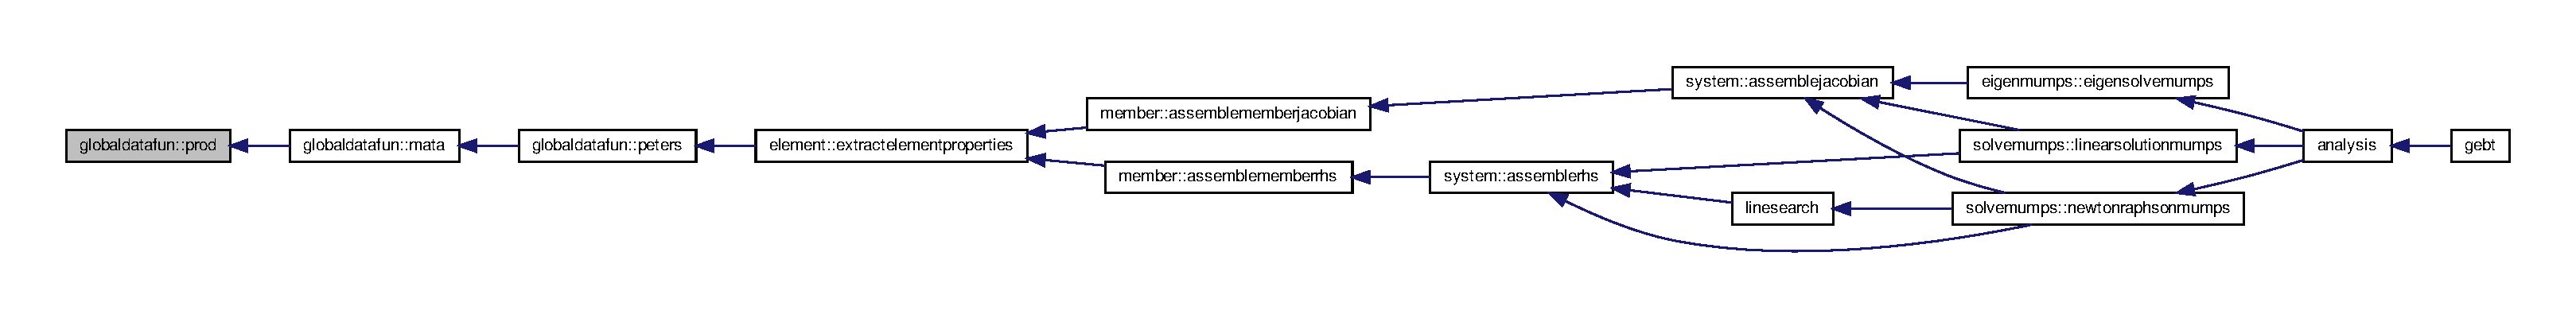
\includegraphics[width=350pt]{namespaceglobaldatafun_afe68f9e5d61e5e7844a0a4b225bb3825_icgraph}
\end{center}
\end{figure}
\mbox{\Hypertarget{namespaceglobaldatafun_aabcfb273a99323881aa160da1f44a561}\label{namespaceglobaldatafun_aabcfb273a99323881aa160da1f44a561}} 
\index{globaldatafun@{globaldatafun}!tilde@{tilde}}
\index{tilde@{tilde}!globaldatafun@{globaldatafun}}
\subsubsection{\texorpdfstring{tilde()}{tilde()}}
{\footnotesize\ttfamily real(\hyperlink{namespaceglobaldatafun_a5008801201dd34f2af8eae07756befb4}{dbl}) function, dimension(3,3), public globaldatafun\+::tilde (\begin{DoxyParamCaption}\item[{real(\hyperlink{namespaceglobaldatafun_a5008801201dd34f2af8eae07756befb4}{dbl}), dimension(3), intent(in)}]{vect }\end{DoxyParamCaption})}



Carry out the tilde operation for a real vector $\ast$. 



Definition at line 625 of file Global\+Data\+Fun.\+f90.

Here is the caller graph for this function\+:\nopagebreak
\begin{figure}[H]
\begin{center}
\leavevmode
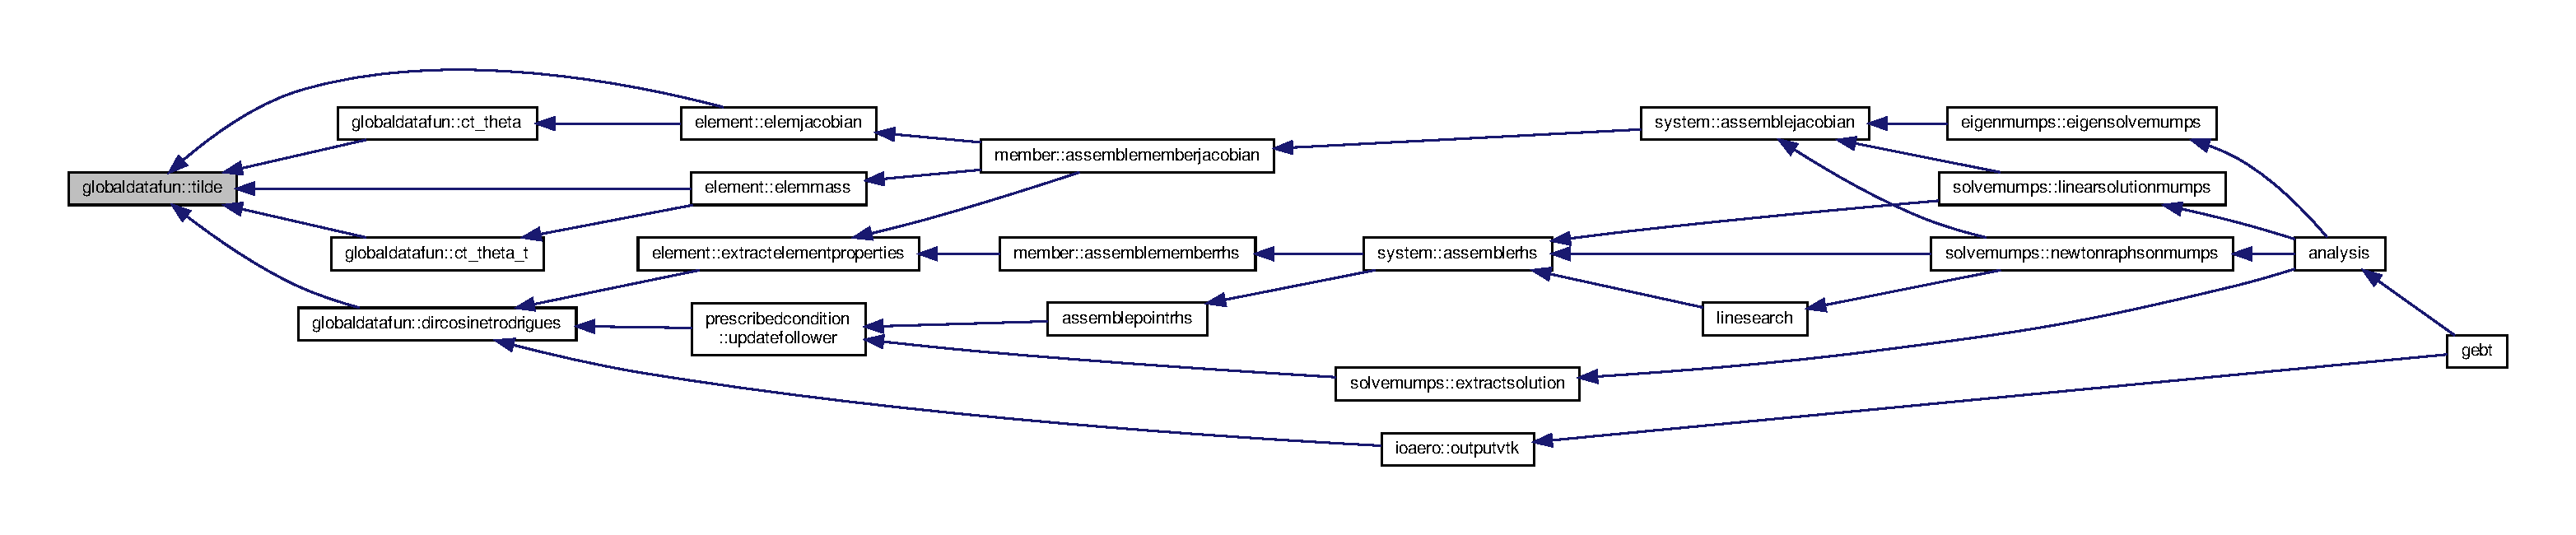
\includegraphics[width=350pt]{namespaceglobaldatafun_aabcfb273a99323881aa160da1f44a561_icgraph}
\end{center}
\end{figure}
\mbox{\Hypertarget{namespaceglobaldatafun_a74b07978d9a6c644031fbb37b131f609}\label{namespaceglobaldatafun_a74b07978d9a6c644031fbb37b131f609}} 
\index{globaldatafun@{globaldatafun}!titleprint@{titleprint}}
\index{titleprint@{titleprint}!globaldatafun@{globaldatafun}}
\subsubsection{\texorpdfstring{titleprint()}{titleprint()}}
{\footnotesize\ttfamily subroutine, public globaldatafun\+::titleprint (\begin{DoxyParamCaption}\item[{integer, intent(in)}]{file\+\_\+unit,  }\item[{character($\ast$), intent(in)}]{title }\end{DoxyParamCaption})}



To print a title for a block of data $\ast$. 



Definition at line 292 of file Global\+Data\+Fun.\+f90.

Here is the caller graph for this function\+:\nopagebreak
\begin{figure}[H]
\begin{center}
\leavevmode
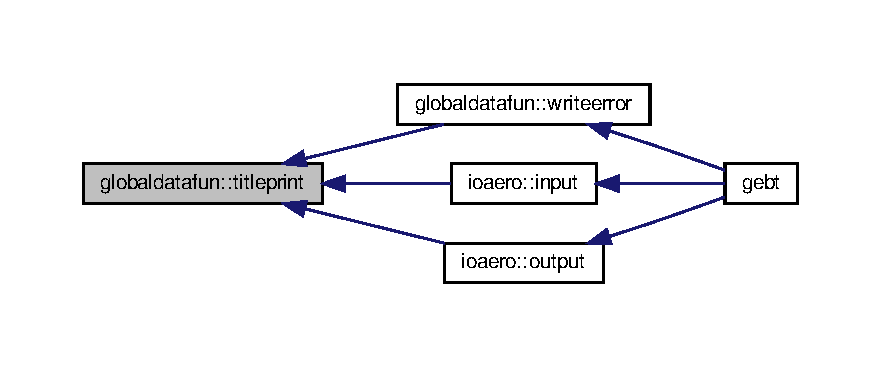
\includegraphics[width=350pt]{namespaceglobaldatafun_a74b07978d9a6c644031fbb37b131f609_icgraph}
\end{center}
\end{figure}
\mbox{\Hypertarget{namespaceglobaldatafun_a0ef3145b88a5e2f7679e5309ed885bc4}\label{namespaceglobaldatafun_a0ef3145b88a5e2f7679e5309ed885bc4}} 
\index{globaldatafun@{globaldatafun}!vecb@{vecb}}
\index{vecb@{vecb}!globaldatafun@{globaldatafun}}
\subsubsection{\texorpdfstring{vecb()}{vecb()}}
{\footnotesize\ttfamily real(\hyperlink{namespaceglobaldatafun_a5008801201dd34f2af8eae07756befb4}{dbl}) function, dimension(n) globaldatafun\+::vecb (\begin{DoxyParamCaption}\item[{integer, intent(in)}]{n }\end{DoxyParamCaption})\hspace{0.3cm}{\ttfamily [private]}}



Compute the Peters B vector. 



Definition at line 825 of file Global\+Data\+Fun.\+f90.

Here is the caller graph for this function\+:\nopagebreak
\begin{figure}[H]
\begin{center}
\leavevmode
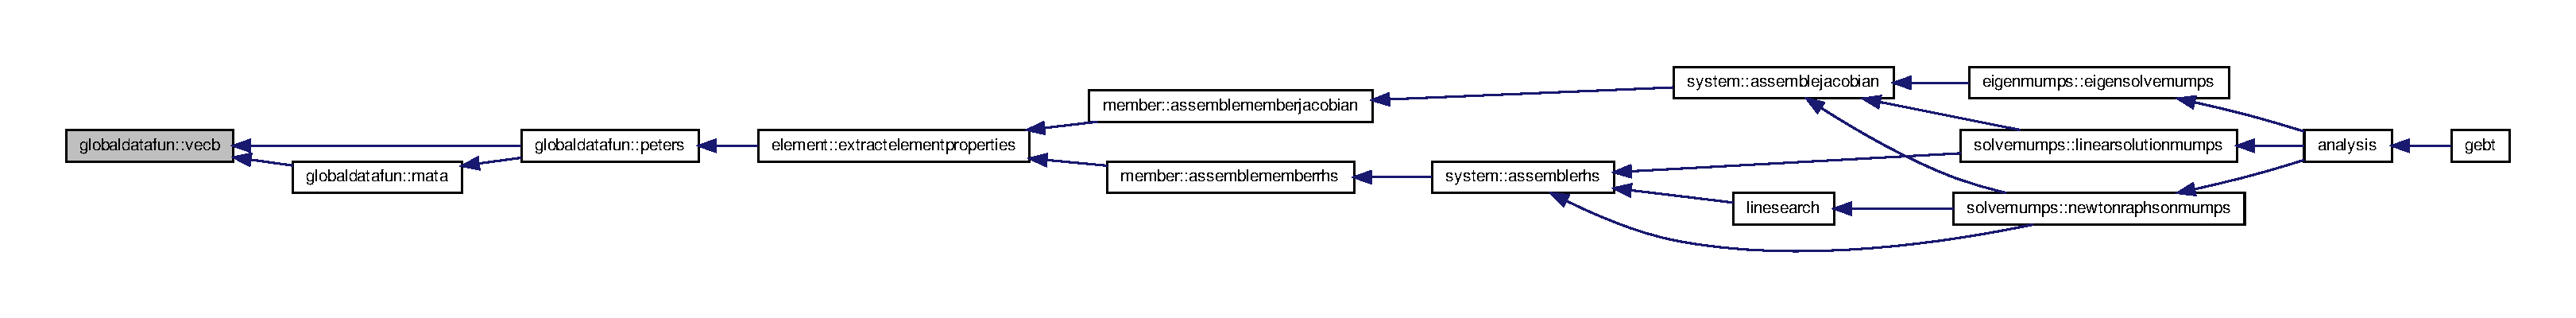
\includegraphics[width=350pt]{namespaceglobaldatafun_a0ef3145b88a5e2f7679e5309ed885bc4_icgraph}
\end{center}
\end{figure}
\mbox{\Hypertarget{namespaceglobaldatafun_ac274536794b3306528c0130a20080b15}\label{namespaceglobaldatafun_ac274536794b3306528c0130a20080b15}} 
\index{globaldatafun@{globaldatafun}!vecc@{vecc}}
\index{vecc@{vecc}!globaldatafun@{globaldatafun}}
\subsubsection{\texorpdfstring{vecc()}{vecc()}}
{\footnotesize\ttfamily real(\hyperlink{namespaceglobaldatafun_a5008801201dd34f2af8eae07756befb4}{dbl}) function, dimension(n) globaldatafun\+::vecc (\begin{DoxyParamCaption}\item[{integer, intent(in)}]{n }\end{DoxyParamCaption})\hspace{0.3cm}{\ttfamily [private]}}



Compute Peters C vector. 



Definition at line 848 of file Global\+Data\+Fun.\+f90.

Here is the caller graph for this function\+:\nopagebreak
\begin{figure}[H]
\begin{center}
\leavevmode
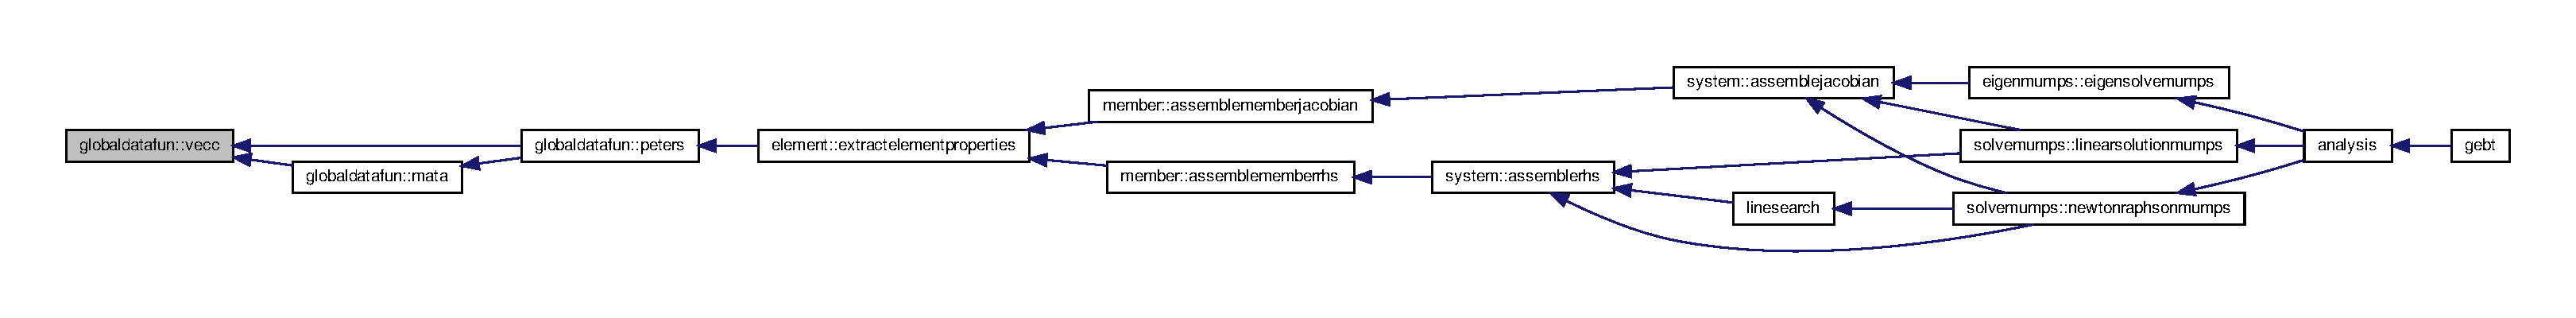
\includegraphics[width=350pt]{namespaceglobaldatafun_ac274536794b3306528c0130a20080b15_icgraph}
\end{center}
\end{figure}
\mbox{\Hypertarget{namespaceglobaldatafun_a71653a1d825c3dee70490c228d23b738}\label{namespaceglobaldatafun_a71653a1d825c3dee70490c228d23b738}} 
\index{globaldatafun@{globaldatafun}!vecd@{vecd}}
\index{vecd@{vecd}!globaldatafun@{globaldatafun}}
\subsubsection{\texorpdfstring{vecd()}{vecd()}}
{\footnotesize\ttfamily real(\hyperlink{namespaceglobaldatafun_a5008801201dd34f2af8eae07756befb4}{dbl}) function, dimension(n) globaldatafun\+::vecd (\begin{DoxyParamCaption}\item[{integer, intent(in)}]{n }\end{DoxyParamCaption})\hspace{0.3cm}{\ttfamily [private]}}



Compute Peters D vector. 



Definition at line 863 of file Global\+Data\+Fun.\+f90.

Here is the caller graph for this function\+:\nopagebreak
\begin{figure}[H]
\begin{center}
\leavevmode
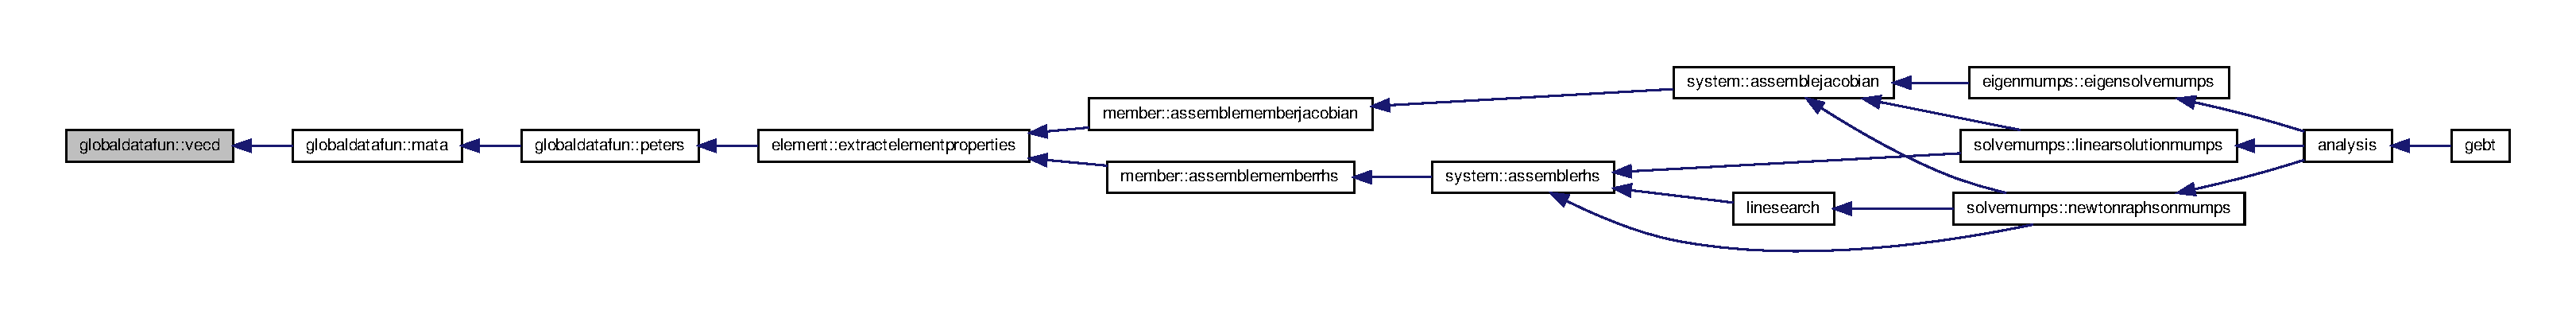
\includegraphics[width=350pt]{namespaceglobaldatafun_a71653a1d825c3dee70490c228d23b738_icgraph}
\end{center}
\end{figure}
\mbox{\Hypertarget{namespaceglobaldatafun_ab8bdea863cb470f4098dbfd74bd27faa}\label{namespaceglobaldatafun_ab8bdea863cb470f4098dbfd74bd27faa}} 
\index{globaldatafun@{globaldatafun}!writeerror@{writeerror}}
\index{writeerror@{writeerror}!globaldatafun@{globaldatafun}}
\subsubsection{\texorpdfstring{writeerror()}{writeerror()}}
{\footnotesize\ttfamily subroutine, public globaldatafun\+::writeerror (\begin{DoxyParamCaption}\item[{integer, intent(in)}]{E\+IN,  }\item[{character($\ast$), intent(in)}]{error }\end{DoxyParamCaption})}



Write error to the echo file $\ast$. 


\begin{DoxyParams}[1]{Parameters}
\mbox{\tt in}  & {\em ein} & file unit to write the error message \\
\hline
\end{DoxyParams}


Definition at line 340 of file Global\+Data\+Fun.\+f90.

Here is the caller graph for this function\+:\nopagebreak
\begin{figure}[H]
\begin{center}
\leavevmode
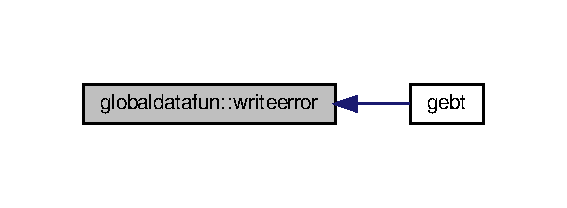
\includegraphics[width=272pt]{namespaceglobaldatafun_ab8bdea863cb470f4098dbfd74bd27faa_icgraph}
\end{center}
\end{figure}
\mbox{\Hypertarget{namespaceglobaldatafun_a08c5dd4cdc68f1694d0d44f76c4df0d5}\label{namespaceglobaldatafun_a08c5dd4cdc68f1694d0d44f76c4df0d5}} 
\index{globaldatafun@{globaldatafun}!writeintvector@{writeintvector}}
\index{writeintvector@{writeintvector}!globaldatafun@{globaldatafun}}
\subsubsection{\texorpdfstring{writeintvector()}{writeintvector()}}
{\footnotesize\ttfamily subroutine globaldatafun\+::writeintvector (\begin{DoxyParamCaption}\item[{integer, intent(in)}]{file\+\_\+unit,  }\item[{integer, dimension(\+:), intent(in)}]{vec }\end{DoxyParamCaption})\hspace{0.3cm}{\ttfamily [private]}}



Write an integer vector to the file\+\_\+unit $\ast$. 


\begin{DoxyParams}[1]{Parameters}
\mbox{\tt in}  & {\em file\+\_\+unit} & File unit to write the vector \\
\hline
\end{DoxyParams}


Definition at line 375 of file Global\+Data\+Fun.\+f90.

\mbox{\Hypertarget{namespaceglobaldatafun_a6a36231350f9af76a3a20cd590f6e40a}\label{namespaceglobaldatafun_a6a36231350f9af76a3a20cd590f6e40a}} 
\index{globaldatafun@{globaldatafun}!writerealvector@{writerealvector}}
\index{writerealvector@{writerealvector}!globaldatafun@{globaldatafun}}
\subsubsection{\texorpdfstring{writerealvector()}{writerealvector()}}
{\footnotesize\ttfamily subroutine globaldatafun\+::writerealvector (\begin{DoxyParamCaption}\item[{integer, intent(in)}]{file\+\_\+unit,  }\item[{real(\hyperlink{namespaceglobaldatafun_a5008801201dd34f2af8eae07756befb4}{dbl}), dimension(\+:), intent(in)}]{vec }\end{DoxyParamCaption})\hspace{0.3cm}{\ttfamily [private]}}



Write a real vector to the file\+\_\+unit $\ast$. 


\begin{DoxyParams}[1]{Parameters}
\mbox{\tt in}  & {\em file\+\_\+unit} & File unit to write the vector \\
\hline
\end{DoxyParams}


Definition at line 392 of file Global\+Data\+Fun.\+f90.



\subsection{Variable Documentation}
\mbox{\Hypertarget{namespaceglobaldatafun_ac0c29e0202eb23daead1a4fcecc645ea}\label{namespaceglobaldatafun_ac0c29e0202eb23daead1a4fcecc645ea}} 
\index{globaldatafun@{globaldatafun}!allo\+\_\+stat@{allo\+\_\+stat}}
\index{allo\+\_\+stat@{allo\+\_\+stat}!globaldatafun@{globaldatafun}}
\subsubsection{\texorpdfstring{allo\+\_\+stat}{allo\_stat}}
{\footnotesize\ttfamily integer, public globaldatafun\+::allo\+\_\+stat}



flag to indicate status of allocating memory 



Definition at line 137 of file Global\+Data\+Fun.\+f90.

\mbox{\Hypertarget{namespaceglobaldatafun_ac1ee1084ba0c21ae53df281847753757}\label{namespaceglobaldatafun_ac1ee1084ba0c21ae53df281847753757}} 
\index{globaldatafun@{globaldatafun}!arpack\+\_\+mod@{arpack\+\_\+mod}}
\index{arpack\+\_\+mod@{arpack\+\_\+mod}!globaldatafun@{globaldatafun}}
\subsubsection{\texorpdfstring{arpack\+\_\+mod}{arpack\_mod}}
{\footnotesize\ttfamily integer, public globaldatafun\+::arpack\+\_\+mod =0}



parameter W\+H\+I\+CH of arpack solver (1\+:LI, 2\+:LM, 3\+:LR, 4\+:SR, default \+: LM in dnaupd and LI in dneupd) =$>$cf Arpack doc 



Definition at line 144 of file Global\+Data\+Fun.\+f90.

\mbox{\Hypertarget{namespaceglobaldatafun_a5008801201dd34f2af8eae07756befb4}\label{namespaceglobaldatafun_a5008801201dd34f2af8eae07756befb4}} 
\index{globaldatafun@{globaldatafun}!dbl@{dbl}}
\index{dbl@{dbl}!globaldatafun@{globaldatafun}}
\subsubsection{\texorpdfstring{dbl}{dbl}}
{\footnotesize\ttfamily integer, parameter, public globaldatafun\+::dbl =S\+E\+L\+E\+C\+T\+E\+D\+\_\+\+R\+E\+A\+L\+\_\+\+K\+I\+ND(15, 307)}



Definition at line 121 of file Global\+Data\+Fun.\+f90.

\mbox{\Hypertarget{namespaceglobaldatafun_a6cd96b1c5754b6f19020fd2ff826086d}\label{namespaceglobaldatafun_a6cd96b1c5754b6f19020fd2ff826086d}} 
\index{globaldatafun@{globaldatafun}!deg\+\_\+2\+\_\+rad@{deg\+\_\+2\+\_\+rad}}
\index{deg\+\_\+2\+\_\+rad@{deg\+\_\+2\+\_\+rad}!globaldatafun@{globaldatafun}}
\subsubsection{\texorpdfstring{deg\+\_\+2\+\_\+rad}{deg\_2\_rad}}
{\footnotesize\ttfamily real(\hyperlink{namespaceglobaldatafun_a5008801201dd34f2af8eae07756befb4}{dbl}), parameter, public globaldatafun\+::deg\+\_\+2\+\_\+rad = 1.\+7453292519943296\+D-\/2}



the ratio between radians and degrees 



Definition at line 124 of file Global\+Data\+Fun.\+f90.

\mbox{\Hypertarget{namespaceglobaldatafun_ae724ce0d8db999ac46505601fee29b3a}\label{namespaceglobaldatafun_ae724ce0d8db999ac46505601fee29b3a}} 
\index{globaldatafun@{globaldatafun}!e1@{e1}}
\index{e1@{e1}!globaldatafun@{globaldatafun}}
\subsubsection{\texorpdfstring{e1}{e1}}
{\footnotesize\ttfamily real(\hyperlink{namespaceglobaldatafun_a5008801201dd34f2af8eae07756befb4}{dbl}), dimension(3), parameter, public globaldatafun\+::e1 =(/1.\+\_\+\+D\+BL,0.\+\_\+\+D\+BL,0.\+\_\+\+D\+BL/)}



The e1 unit vector. 



Definition at line 132 of file Global\+Data\+Fun.\+f90.

\mbox{\Hypertarget{namespaceglobaldatafun_a312b192a05c2e5b3dd301528abdba07c}\label{namespaceglobaldatafun_a312b192a05c2e5b3dd301528abdba07c}} 
\index{globaldatafun@{globaldatafun}!eigen\+\_\+output@{eigen\+\_\+output}}
\index{eigen\+\_\+output@{eigen\+\_\+output}!globaldatafun@{globaldatafun}}
\subsubsection{\texorpdfstring{eigen\+\_\+output}{eigen\_output}}
{\footnotesize\ttfamily integer, public globaldatafun\+::eigen\+\_\+output =0}



define wich eigenvalue data to output (0\+: eigenvalues and eigenvectors, 1\+: eigenvalues only) 



Definition at line 145 of file Global\+Data\+Fun.\+f90.

\mbox{\Hypertarget{namespaceglobaldatafun_a71be24aec97056093e319698ed6df6fd}\label{namespaceglobaldatafun_a71be24aec97056093e319698ed6df6fd}} 
\index{globaldatafun@{globaldatafun}!flutter\+\_\+flag@{flutter\+\_\+flag}}
\index{flutter\+\_\+flag@{flutter\+\_\+flag}!globaldatafun@{globaldatafun}}
\subsubsection{\texorpdfstring{flutter\+\_\+flag}{flutter\_flag}}
{\footnotesize\ttfamily integer, public globaldatafun\+::flutter\+\_\+flag =0}



used in temporal simulation \+: 0= deformation are under a \char`\"{}flutter\char`\"{} state; 1= deformation are over a \char`\"{}flutter\char`\"{} state 



Definition at line 147 of file Global\+Data\+Fun.\+f90.

\mbox{\Hypertarget{namespaceglobaldatafun_a00437dc044a340393bafc8c15d696e7a}\label{namespaceglobaldatafun_a00437dc044a340393bafc8c15d696e7a}} 
\index{globaldatafun@{globaldatafun}!flutter\+\_\+limit@{flutter\+\_\+limit}}
\index{flutter\+\_\+limit@{flutter\+\_\+limit}!globaldatafun@{globaldatafun}}
\subsubsection{\texorpdfstring{flutter\+\_\+limit}{flutter\_limit}}
{\footnotesize\ttfamily real(\hyperlink{namespaceglobaldatafun_a5008801201dd34f2af8eae07756befb4}{dbl}), public globaldatafun\+::flutter\+\_\+limit}



the value of maximale angular deformaton use to trigger the flutter flag 



Definition at line 148 of file Global\+Data\+Fun.\+f90.

\mbox{\Hypertarget{namespaceglobaldatafun_a9636e338fbbaf3b710c9483f5ba825ad}\label{namespaceglobaldatafun_a9636e338fbbaf3b710c9483f5ba825ad}} 
\index{globaldatafun@{globaldatafun}!fmt\+\_\+int@{fmt\+\_\+int}}
\index{fmt\+\_\+int@{fmt\+\_\+int}!globaldatafun@{globaldatafun}}
\subsubsection{\texorpdfstring{fmt\+\_\+int}{fmt\_int}}
{\footnotesize\ttfamily character($\ast$), parameter, public globaldatafun\+::fmt\+\_\+int =\textquotesingle{}I8\textquotesingle{}}



format for output integer numbers 



Definition at line 141 of file Global\+Data\+Fun.\+f90.

\mbox{\Hypertarget{namespaceglobaldatafun_ab9b7950cc6b98bba6c90ccbc0bf16763}\label{namespaceglobaldatafun_ab9b7950cc6b98bba6c90ccbc0bf16763}} 
\index{globaldatafun@{globaldatafun}!fmt\+\_\+real@{fmt\+\_\+real}}
\index{fmt\+\_\+real@{fmt\+\_\+real}!globaldatafun@{globaldatafun}}
\subsubsection{\texorpdfstring{fmt\+\_\+real}{fmt\_real}}
{\footnotesize\ttfamily character($\ast$), parameter, public globaldatafun\+::fmt\+\_\+real =\textquotesingle{}E\+S15.\+7\textquotesingle{}}



format for output real numbers 



Definition at line 140 of file Global\+Data\+Fun.\+f90.

\mbox{\Hypertarget{namespaceglobaldatafun_a6ddc394879657b50856a10648f3af6bd}\label{namespaceglobaldatafun_a6ddc394879657b50856a10648f3af6bd}} 
\index{globaldatafun@{globaldatafun}!grav@{grav}}
\index{grav@{grav}!globaldatafun@{globaldatafun}}
\subsubsection{\texorpdfstring{grav}{grav}}
{\footnotesize\ttfamily real(\hyperlink{namespaceglobaldatafun_a5008801201dd34f2af8eae07756befb4}{dbl}), parameter, public globaldatafun\+::grav = 9.\+81}



gravity acceleration 



Definition at line 127 of file Global\+Data\+Fun.\+f90.

\mbox{\Hypertarget{namespaceglobaldatafun_abe3df2088f071e903ebdcf4734f6dc27}\label{namespaceglobaldatafun_abe3df2088f071e903ebdcf4734f6dc27}} 
\index{globaldatafun@{globaldatafun}!i3@{i3}}
\index{i3@{i3}!globaldatafun@{globaldatafun}}
\subsubsection{\texorpdfstring{i3}{i3}}
{\footnotesize\ttfamily real(\hyperlink{namespaceglobaldatafun_a5008801201dd34f2af8eae07756befb4}{dbl}), dimension(3,3), parameter, public globaldatafun\+::i3 = R\+E\+S\+H\+A\+PE((/1.D0, 0.D0, 0.D0, 0.D0, 1.D0, 0.D0, 0.D0, 0.D0, 1.D0/), (/3,3/))}



The 3x3 identity matrix. 



Definition at line 129 of file Global\+Data\+Fun.\+f90.

\mbox{\Hypertarget{namespaceglobaldatafun_a64c0718f56f06c9fe3cfb49b0dc5ced0}\label{namespaceglobaldatafun_a64c0718f56f06c9fe3cfb49b0dc5ced0}} 
\index{globaldatafun@{globaldatafun}!in\+\_\+stat@{in\+\_\+stat}}
\index{in\+\_\+stat@{in\+\_\+stat}!globaldatafun@{globaldatafun}}
\subsubsection{\texorpdfstring{in\+\_\+stat}{in\_stat}}
{\footnotesize\ttfamily integer, public globaldatafun\+::in\+\_\+stat}



flag to indicate if the I/O process is successful\+: if positive, an error occured; if negative, an end-\/of-\/file or end-\/of-\/record condition occurred; zero, no error, end-\/of-\/file, or end-\/of-\/record condition occurred. 



Definition at line 134 of file Global\+Data\+Fun.\+f90.

\mbox{\Hypertarget{namespaceglobaldatafun_ae88f4c5de30b425e43d5392116dfdcda}\label{namespaceglobaldatafun_ae88f4c5de30b425e43d5392116dfdcda}} 
\index{globaldatafun@{globaldatafun}!memb\+\_\+const@{memb\+\_\+const}}
\index{memb\+\_\+const@{memb\+\_\+const}!globaldatafun@{globaldatafun}}
\subsubsection{\texorpdfstring{memb\+\_\+const}{memb\_const}}
{\footnotesize\ttfamily integer, parameter, public globaldatafun\+::memb\+\_\+const =7}



Number of labels needed for member properties. 



Definition at line 118 of file Global\+Data\+Fun.\+f90.

\mbox{\Hypertarget{namespaceglobaldatafun_a5041a6e08575b124a458c49a76dc6d31}\label{namespaceglobaldatafun_a5041a6e08575b124a458c49a76dc6d31}} 
\index{globaldatafun@{globaldatafun}!ndim@{ndim}}
\index{ndim@{ndim}!globaldatafun@{globaldatafun}}
\subsubsection{\texorpdfstring{ndim}{ndim}}
{\footnotesize\ttfamily integer, parameter, public globaldatafun\+::ndim =3}



All the beams could behavior in the 3D space. 



Definition at line 115 of file Global\+Data\+Fun.\+f90.

\mbox{\Hypertarget{namespaceglobaldatafun_a44ab75808fb35a144d54fa9a6c9fe07a}\label{namespaceglobaldatafun_a44ab75808fb35a144d54fa9a6c9fe07a}} 
\index{globaldatafun@{globaldatafun}!ndof\+\_\+nd@{ndof\+\_\+nd}}
\index{ndof\+\_\+nd@{ndof\+\_\+nd}!globaldatafun@{globaldatafun}}
\subsubsection{\texorpdfstring{ndof\+\_\+nd}{ndof\_nd}}
{\footnotesize\ttfamily integer, parameter, public globaldatafun\+::ndof\+\_\+nd =12}



degrees of freedom per node/element is 12. 



Definition at line 116 of file Global\+Data\+Fun.\+f90.

\mbox{\Hypertarget{namespaceglobaldatafun_a2c33dd8d5d818282893dd132f6b33564}\label{namespaceglobaldatafun_a2c33dd8d5d818282893dd132f6b33564}} 
\index{globaldatafun@{globaldatafun}!nstates@{nstates}}
\index{nstates@{nstates}!globaldatafun@{globaldatafun}}
\subsubsection{\texorpdfstring{nstates}{nstates}}
{\footnotesize\ttfamily integer, parameter, public globaldatafun\+::nstates = 6}



Number of induces-\/flow states in Peters theory. 



Definition at line 119 of file Global\+Data\+Fun.\+f90.

\mbox{\Hypertarget{namespaceglobaldatafun_a3aff613607f0e62fc5c5739e9f2432e9}\label{namespaceglobaldatafun_a3aff613607f0e62fc5c5739e9f2432e9}} 
\index{globaldatafun@{globaldatafun}!nstrn@{nstrn}}
\index{nstrn@{nstrn}!globaldatafun@{globaldatafun}}
\subsubsection{\texorpdfstring{nstrn}{nstrn}}
{\footnotesize\ttfamily integer, parameter, public globaldatafun\+::nstrn =6}



Number of strain measures/dofs in Timoshenko model. 



Definition at line 117 of file Global\+Data\+Fun.\+f90.

\mbox{\Hypertarget{namespaceglobaldatafun_a05144a47841796a672385a1db57f91a1}\label{namespaceglobaldatafun_a05144a47841796a672385a1db57f91a1}} 
\index{globaldatafun@{globaldatafun}!pi@{pi}}
\index{pi@{pi}!globaldatafun@{globaldatafun}}
\subsubsection{\texorpdfstring{pi}{pi}}
{\footnotesize\ttfamily real(\hyperlink{namespaceglobaldatafun_a5008801201dd34f2af8eae07756befb4}{dbl}), parameter, public globaldatafun\+::pi = 3.\+1415926535897932\+D0}



Definition at line 123 of file Global\+Data\+Fun.\+f90.

\mbox{\Hypertarget{namespaceglobaldatafun_a65560765d885097ca1432983f9cf6bab}\label{namespaceglobaldatafun_a65560765d885097ca1432983f9cf6bab}} 
\index{globaldatafun@{globaldatafun}!rad\+\_\+2\+\_\+deg@{rad\+\_\+2\+\_\+deg}}
\index{rad\+\_\+2\+\_\+deg@{rad\+\_\+2\+\_\+deg}!globaldatafun@{globaldatafun}}
\subsubsection{\texorpdfstring{rad\+\_\+2\+\_\+deg}{rad\_2\_deg}}
{\footnotesize\ttfamily real(\hyperlink{namespaceglobaldatafun_a5008801201dd34f2af8eae07756befb4}{dbl}), parameter, public globaldatafun\+::rad\+\_\+2\+\_\+deg = 5.\+7295779513082321\+D1}



convert radian to degree 



Definition at line 125 of file Global\+Data\+Fun.\+f90.

\mbox{\Hypertarget{namespaceglobaldatafun_a69fb7d8f3bbcc95ea17d1f924b50fbfa}\label{namespaceglobaldatafun_a69fb7d8f3bbcc95ea17d1f924b50fbfa}} 
\index{globaldatafun@{globaldatafun}!runmod@{runmod}}
\index{runmod@{runmod}!globaldatafun@{globaldatafun}}
\subsubsection{\texorpdfstring{runmod}{runmod}}
{\footnotesize\ttfamily integer, public globaldatafun\+::runmod =0}



Define the output behavior of the program; 0\+: legacy mode of the computation code with output of a .out text file; 1\+: mode compatible with the python pre/postrpocessor (argument -\/p in the terminal), 2\+: silent mode (argument -\/s in the terminal) 



Definition at line 143 of file Global\+Data\+Fun.\+f90.

\mbox{\Hypertarget{namespaceglobaldatafun_a895a1e10c59021323fcf518893f6c0de}\label{namespaceglobaldatafun_a895a1e10c59021323fcf518893f6c0de}} 
\index{globaldatafun@{globaldatafun}!solver@{solver}}
\index{solver@{solver}!globaldatafun@{globaldatafun}}
\subsubsection{\texorpdfstring{solver}{solver}}
{\footnotesize\ttfamily character(10), public globaldatafun\+::solver =\textquotesingle{}M\+U\+M\+PS\textquotesingle{}}



linear solver used (H\+SL \+: ddep.\+f, mc19.\+f + ma28 or M\+U\+M\+PS \+: linux library) 



Definition at line 146 of file Global\+Data\+Fun.\+f90.

\mbox{\Hypertarget{namespaceglobaldatafun_a163afcd0caf3537efef266782e451784}\label{namespaceglobaldatafun_a163afcd0caf3537efef266782e451784}} 
\index{globaldatafun@{globaldatafun}!tolerance@{tolerance}}
\index{tolerance@{tolerance}!globaldatafun@{globaldatafun}}
\subsubsection{\texorpdfstring{tolerance}{tolerance}}
{\footnotesize\ttfamily real(\hyperlink{namespaceglobaldatafun_a5008801201dd34f2af8eae07756befb4}{dbl}), parameter, public globaldatafun\+::tolerance = E\+P\+S\+I\+L\+ON(1.\+0\+\_\+\+D\+B\+L)}



a smart number of the double precision real number 



Definition at line 126 of file Global\+Data\+Fun.\+f90.


\hypertarget{namespaceinternaldata}{}\section{internaldata Module Reference}
\label{namespaceinternaldata}\index{internaldata@{internaldata}}


This module contains the variables needed internally in the program. Not necessary to be defined in the outside environment.  


\subsection*{Data Types}
\begin{DoxyCompactItemize}
\item 
type \hyperlink{structinternaldata_1_1memberinf}{memberinf}
\begin{DoxyCompactList}\small\item\em structure containing the caracteritics of a finite element. \end{DoxyCompactList}\end{DoxyCompactItemize}
\subsection*{Variables}
\begin{DoxyCompactItemize}
\item 
logical, parameter \hyperlink{namespaceinternaldata_a0c3051eb2c273aad5bebc55fd79236ea}{debug} =.F\+A\+L\+S\+E.
\item 
integer, parameter \hyperlink{namespaceinternaldata_a82858bed9f1804b4d9d545add41703b8}{iout} =30
\item 
character(64) \hyperlink{namespaceinternaldata_abe3cfd1606a2a73e5e71421a1abc89dd}{deb\+\_\+name}
\item 
integer \hyperlink{namespaceinternaldata_a870ff06e13dc622293c20b2cc20641b9}{nsize}
\item 
integer, dimension(\+:,\+:), allocatable \hyperlink{namespaceinternaldata_a64b1e517fcf8a25bce3446ec324a4698}{dof\+\_\+all}
\item 
integer, dimension(\+:,\+:), allocatable \hyperlink{namespaceinternaldata_a2037100926e06d16be5b80c12d0c36e9}{follower\+\_\+all}
\item 
real(dbl), dimension(\+:,\+:), allocatable \hyperlink{namespaceinternaldata_aeb804e680e34df79573f79272474bd2c}{cond\+\_\+all}
\item 
real(dbl), dimension(\+:,\+:), allocatable \hyperlink{namespaceinternaldata_a187a3d4ecc99e732bd15234944dae732}{init\+\_\+memb}
\item 
integer \hyperlink{namespaceinternaldata_accc2e120df220e17a9e2b6cc72e42793}{init\+\_\+flag}
\item 
real(dbl) \hyperlink{namespaceinternaldata_a6c7ccd03dc69209443b0d6756c26f43a}{two\+\_\+divide\+\_\+dt}
\begin{DoxyCompactList}\small\item\em 2/dt \end{DoxyCompactList}\item 
integer \hyperlink{namespaceinternaldata_ae1ae8091a874c45a6efe110578e140bc}{assemble\+\_\+flag} =0
\begin{DoxyCompactList}\small\item\em for the purpose to share the routines between assembly of stiffness matrix and mass matrix \end{DoxyCompactList}\item 
integer, dimension(\+:,\+:), allocatable \hyperlink{namespaceinternaldata_af8b2fe1b76c22e0b7ae0cb514d52b04f}{index\+\_\+kp}
\begin{DoxyCompactList}\small\item\em the starting row and column for each kp \end{DoxyCompactList}\item 
integer, dimension(\+:,\+:), allocatable \hyperlink{namespaceinternaldata_ac5f95d07b735be7220fcf6814e1ab4a8}{index\+\_\+mb}
\begin{DoxyCompactList}\small\item\em the starting row and column for each member \end{DoxyCompactList}\item 
real(dbl), dimension(ndim) \hyperlink{namespaceinternaldata_a9ea25e6f8fbdc09124cc1002446ffcfc}{xyz\+\_\+pt1}
\begin{DoxyCompactList}\small\item\em the coordinate of the starting point of the first member \end{DoxyCompactList}\item 
integer, parameter \hyperlink{namespaceinternaldata_ac1eede24bc6cba1bdab331c6ad695fcc}{nzelemmax} =500
\item 
integer \hyperlink{namespaceinternaldata_a9f8cf693f79f58344704c979aa5168c4}{nemax}
\end{DoxyCompactItemize}


\subsection{Detailed Description}
This module contains the variables needed internally in the program. Not necessary to be defined in the outside environment. 

\subsection{Variable Documentation}
\mbox{\Hypertarget{namespaceinternaldata_ae1ae8091a874c45a6efe110578e140bc}\label{namespaceinternaldata_ae1ae8091a874c45a6efe110578e140bc}} 
\index{internaldata@{internaldata}!assemble\+\_\+flag@{assemble\+\_\+flag}}
\index{assemble\+\_\+flag@{assemble\+\_\+flag}!internaldata@{internaldata}}
\subsubsection{\texorpdfstring{assemble\+\_\+flag}{assemble\_flag}}
{\footnotesize\ttfamily integer internaldata\+::assemble\+\_\+flag =0}



for the purpose to share the routines between assembly of stiffness matrix and mass matrix 



Definition at line 47 of file Internal\+Data.\+f90.

\mbox{\Hypertarget{namespaceinternaldata_aeb804e680e34df79573f79272474bd2c}\label{namespaceinternaldata_aeb804e680e34df79573f79272474bd2c}} 
\index{internaldata@{internaldata}!cond\+\_\+all@{cond\+\_\+all}}
\index{cond\+\_\+all@{cond\+\_\+all}!internaldata@{internaldata}}
\subsubsection{\texorpdfstring{cond\+\_\+all}{cond\_all}}
{\footnotesize\ttfamily real(dbl), dimension(\+:,\+:), allocatable internaldata\+::cond\+\_\+all}



Definition at line 41 of file Internal\+Data.\+f90.

\mbox{\Hypertarget{namespaceinternaldata_abe3cfd1606a2a73e5e71421a1abc89dd}\label{namespaceinternaldata_abe3cfd1606a2a73e5e71421a1abc89dd}} 
\index{internaldata@{internaldata}!deb\+\_\+name@{deb\+\_\+name}}
\index{deb\+\_\+name@{deb\+\_\+name}!internaldata@{internaldata}}
\subsubsection{\texorpdfstring{deb\+\_\+name}{deb\_name}}
{\footnotesize\ttfamily character(64) internaldata\+::deb\+\_\+name}



Definition at line 30 of file Internal\+Data.\+f90.

\mbox{\Hypertarget{namespaceinternaldata_a0c3051eb2c273aad5bebc55fd79236ea}\label{namespaceinternaldata_a0c3051eb2c273aad5bebc55fd79236ea}} 
\index{internaldata@{internaldata}!debug@{debug}}
\index{debug@{debug}!internaldata@{internaldata}}
\subsubsection{\texorpdfstring{debug}{debug}}
{\footnotesize\ttfamily logical, parameter internaldata\+::debug =.F\+A\+L\+S\+E.}



Definition at line 25 of file Internal\+Data.\+f90.

\mbox{\Hypertarget{namespaceinternaldata_a64b1e517fcf8a25bce3446ec324a4698}\label{namespaceinternaldata_a64b1e517fcf8a25bce3446ec324a4698}} 
\index{internaldata@{internaldata}!dof\+\_\+all@{dof\+\_\+all}}
\index{dof\+\_\+all@{dof\+\_\+all}!internaldata@{internaldata}}
\subsubsection{\texorpdfstring{dof\+\_\+all}{dof\_all}}
{\footnotesize\ttfamily integer, dimension(\+:,\+:), allocatable internaldata\+::dof\+\_\+all}



Definition at line 39 of file Internal\+Data.\+f90.

\mbox{\Hypertarget{namespaceinternaldata_a2037100926e06d16be5b80c12d0c36e9}\label{namespaceinternaldata_a2037100926e06d16be5b80c12d0c36e9}} 
\index{internaldata@{internaldata}!follower\+\_\+all@{follower\+\_\+all}}
\index{follower\+\_\+all@{follower\+\_\+all}!internaldata@{internaldata}}
\subsubsection{\texorpdfstring{follower\+\_\+all}{follower\_all}}
{\footnotesize\ttfamily integer, dimension(\+:,\+:), allocatable internaldata\+::follower\+\_\+all}



Definition at line 40 of file Internal\+Data.\+f90.

\mbox{\Hypertarget{namespaceinternaldata_af8b2fe1b76c22e0b7ae0cb514d52b04f}\label{namespaceinternaldata_af8b2fe1b76c22e0b7ae0cb514d52b04f}} 
\index{internaldata@{internaldata}!index\+\_\+kp@{index\+\_\+kp}}
\index{index\+\_\+kp@{index\+\_\+kp}!internaldata@{internaldata}}
\subsubsection{\texorpdfstring{index\+\_\+kp}{index\_kp}}
{\footnotesize\ttfamily integer, dimension(\+:,\+:), allocatable internaldata\+::index\+\_\+kp}



the starting row and column for each kp 



Definition at line 48 of file Internal\+Data.\+f90.

\mbox{\Hypertarget{namespaceinternaldata_ac5f95d07b735be7220fcf6814e1ab4a8}\label{namespaceinternaldata_ac5f95d07b735be7220fcf6814e1ab4a8}} 
\index{internaldata@{internaldata}!index\+\_\+mb@{index\+\_\+mb}}
\index{index\+\_\+mb@{index\+\_\+mb}!internaldata@{internaldata}}
\subsubsection{\texorpdfstring{index\+\_\+mb}{index\_mb}}
{\footnotesize\ttfamily integer, dimension(\+:,\+:), allocatable internaldata\+::index\+\_\+mb}



the starting row and column for each member 



Definition at line 49 of file Internal\+Data.\+f90.

\mbox{\Hypertarget{namespaceinternaldata_accc2e120df220e17a9e2b6cc72e42793}\label{namespaceinternaldata_accc2e120df220e17a9e2b6cc72e42793}} 
\index{internaldata@{internaldata}!init\+\_\+flag@{init\+\_\+flag}}
\index{init\+\_\+flag@{init\+\_\+flag}!internaldata@{internaldata}}
\subsubsection{\texorpdfstring{init\+\_\+flag}{init\_flag}}
{\footnotesize\ttfamily integer internaldata\+::init\+\_\+flag}



Definition at line 45 of file Internal\+Data.\+f90.

\mbox{\Hypertarget{namespaceinternaldata_a187a3d4ecc99e732bd15234944dae732}\label{namespaceinternaldata_a187a3d4ecc99e732bd15234944dae732}} 
\index{internaldata@{internaldata}!init\+\_\+memb@{init\+\_\+memb}}
\index{init\+\_\+memb@{init\+\_\+memb}!internaldata@{internaldata}}
\subsubsection{\texorpdfstring{init\+\_\+memb}{init\_memb}}
{\footnotesize\ttfamily real(dbl), dimension(\+:,\+:), allocatable internaldata\+::init\+\_\+memb}



Definition at line 43 of file Internal\+Data.\+f90.

\mbox{\Hypertarget{namespaceinternaldata_a82858bed9f1804b4d9d545add41703b8}\label{namespaceinternaldata_a82858bed9f1804b4d9d545add41703b8}} 
\index{internaldata@{internaldata}!iout@{iout}}
\index{iout@{iout}!internaldata@{internaldata}}
\subsubsection{\texorpdfstring{iout}{iout}}
{\footnotesize\ttfamily integer, parameter internaldata\+::iout =30}



Definition at line 29 of file Internal\+Data.\+f90.

\mbox{\Hypertarget{namespaceinternaldata_a9f8cf693f79f58344704c979aa5168c4}\label{namespaceinternaldata_a9f8cf693f79f58344704c979aa5168c4}} 
\index{internaldata@{internaldata}!nemax@{nemax}}
\index{nemax@{nemax}!internaldata@{internaldata}}
\subsubsection{\texorpdfstring{nemax}{nemax}}
{\footnotesize\ttfamily integer internaldata\+::nemax}



Definition at line 65 of file Internal\+Data.\+f90.

\mbox{\Hypertarget{namespaceinternaldata_a870ff06e13dc622293c20b2cc20641b9}\label{namespaceinternaldata_a870ff06e13dc622293c20b2cc20641b9}} 
\index{internaldata@{internaldata}!nsize@{nsize}}
\index{nsize@{nsize}!internaldata@{internaldata}}
\subsubsection{\texorpdfstring{nsize}{nsize}}
{\footnotesize\ttfamily integer internaldata\+::nsize}



Definition at line 34 of file Internal\+Data.\+f90.

\mbox{\Hypertarget{namespaceinternaldata_ac1eede24bc6cba1bdab331c6ad695fcc}\label{namespaceinternaldata_ac1eede24bc6cba1bdab331c6ad695fcc}} 
\index{internaldata@{internaldata}!nzelemmax@{nzelemmax}}
\index{nzelemmax@{nzelemmax}!internaldata@{internaldata}}
\subsubsection{\texorpdfstring{nzelemmax}{nzelemmax}}
{\footnotesize\ttfamily integer, parameter internaldata\+::nzelemmax =500}



Definition at line 63 of file Internal\+Data.\+f90.

\mbox{\Hypertarget{namespaceinternaldata_a6c7ccd03dc69209443b0d6756c26f43a}\label{namespaceinternaldata_a6c7ccd03dc69209443b0d6756c26f43a}} 
\index{internaldata@{internaldata}!two\+\_\+divide\+\_\+dt@{two\+\_\+divide\+\_\+dt}}
\index{two\+\_\+divide\+\_\+dt@{two\+\_\+divide\+\_\+dt}!internaldata@{internaldata}}
\subsubsection{\texorpdfstring{two\+\_\+divide\+\_\+dt}{two\_divide\_dt}}
{\footnotesize\ttfamily real(dbl) internaldata\+::two\+\_\+divide\+\_\+dt}



2/dt 



Definition at line 46 of file Internal\+Data.\+f90.

\mbox{\Hypertarget{namespaceinternaldata_a9ea25e6f8fbdc09124cc1002446ffcfc}\label{namespaceinternaldata_a9ea25e6f8fbdc09124cc1002446ffcfc}} 
\index{internaldata@{internaldata}!xyz\+\_\+pt1@{xyz\+\_\+pt1}}
\index{xyz\+\_\+pt1@{xyz\+\_\+pt1}!internaldata@{internaldata}}
\subsubsection{\texorpdfstring{xyz\+\_\+pt1}{xyz\_pt1}}
{\footnotesize\ttfamily real(dbl), dimension(ndim) internaldata\+::xyz\+\_\+pt1}



the coordinate of the starting point of the first member 



Definition at line 50 of file Internal\+Data.\+f90.


\hypertarget{namespaceioaero}{}\section{ioaero Module Reference}
\label{namespaceioaero}\index{ioaero@{ioaero}}


This module handle I/O of the computation code. Allow to read a .dat command file possibly with a .ini file and output a .out text output file or/and a folder with .vtk file intended to be used with paraview.  


\subsection*{Functions/\+Subroutines}
\begin{DoxyCompactItemize}
\item 
subroutine, public \hyperlink{namespaceioaero_a039bc1aae10012ce8e368bc202bb81be}{input}
\item 
subroutine, public \hyperlink{namespaceioaero_a1f2f8f2b4f6e233d2753c1fd1809a44a}{output}
\item 
subroutine, public \hyperlink{namespaceioaero_a7eb68cb1588d24e05c8f056ca107e163}{outputvtk}
\end{DoxyCompactItemize}
\subsection*{Variables}
\begin{DoxyCompactItemize}
\item 
integer, parameter, private \hyperlink{namespaceioaero_acd6bdfdcfd986fd1c26261e5996e3b03}{char\+\_\+len} =256
\item 
integer, parameter \hyperlink{namespaceioaero_a09d53f15b1a2c723ad2b4df01c16bccc}{in} =10
\item 
character(\hyperlink{namespaceioaero_acd6bdfdcfd986fd1c26261e5996e3b03}{char\+\_\+len}) \hyperlink{namespaceioaero_ae3b39e5c092106ddc3bb8b81daf8bd13}{inp\+\_\+name}
\item 
integer, parameter, public \hyperlink{namespaceioaero_a6a4b9f5362e2eee64e5777786065f563}{ein} =20
\begin{DoxyCompactList}\small\item\em file for echoing the inputs\+: inp\+\_\+name.\+ech \end{DoxyCompactList}\item 
character(\hyperlink{namespaceioaero_acd6bdfdcfd986fd1c26261e5996e3b03}{char\+\_\+len}+3) \hyperlink{namespaceioaero_a175dde142a22987a0e59b9738444d2e3}{ech\+\_\+name}
\item 
integer, parameter \hyperlink{namespaceioaero_a7c01d4bcd841d8d6281f29d5fc818fd8}{out} =40
\begin{DoxyCompactList}\small\item\em file for output\+: inp\+\_\+name.\+out \end{DoxyCompactList}\item 
character(\hyperlink{namespaceioaero_acd6bdfdcfd986fd1c26261e5996e3b03}{char\+\_\+len}+3) \hyperlink{namespaceioaero_a6693b9440660a84d2d2fc41ac183bb0f}{out\+\_\+name}
\item 
integer, parameter \hyperlink{namespaceioaero_afb3050696f2887599d4083672103b6e7}{init} =50
\begin{DoxyCompactList}\small\item\em file for initial conditions\+: inp\+\_\+name.\+ini \end{DoxyCompactList}\item 
character(\hyperlink{namespaceioaero_acd6bdfdcfd986fd1c26261e5996e3b03}{char\+\_\+len}+3) \hyperlink{namespaceioaero_a5a12b8b21f86b26e7364428778a85d0b}{init\+\_\+name}
\item 
integer, public \hyperlink{namespaceioaero_a24506866304c39bd1fa57ef73b124335}{nkp}
\begin{DoxyCompactList}\small\item\em number of key points \end{DoxyCompactList}\item 
integer, public \hyperlink{namespaceioaero_a543ebf3623a96606d0956211621ce254}{nelem}
\begin{DoxyCompactList}\small\item\em total number of elements \end{DoxyCompactList}\item 
integer, public \hyperlink{namespaceioaero_ab59096c14b19d71fd53523822067402c}{nmemb}
\begin{DoxyCompactList}\small\item\em number of members \end{DoxyCompactList}\item 
integer, public \hyperlink{namespaceioaero_ad8817641275f11b821b7720a78651531}{nmate}
\begin{DoxyCompactList}\small\item\em number of cross-\/sectional properties sets \end{DoxyCompactList}\item 
integer, public \hyperlink{namespaceioaero_ac9fe2ddcc0797f81e7bc475a28692978}{nframe}
\begin{DoxyCompactList}\small\item\em number of frames \end{DoxyCompactList}\item 
integer, public \hyperlink{namespaceioaero_a5ffc5d3578d9abad99d3736ba352e07d}{ncond\+\_\+pt}
\begin{DoxyCompactList}\small\item\em number of point conditions for concentrated loads and boundary conditions \end{DoxyCompactList}\item 
integer, public \hyperlink{namespaceioaero_a89e1f8f2d6913d23ef482a5788d2eba5}{ndistrfun}
\begin{DoxyCompactList}\small\item\em number of distributed functions \end{DoxyCompactList}\item 
integer, public \hyperlink{namespaceioaero_a34dabcb4bc1b4f260277297856ac3653}{ncurv}
\begin{DoxyCompactList}\small\item\em number of initial curvatures/twists \end{DoxyCompactList}\item 
integer, public \hyperlink{namespaceioaero_a435527b09d62e7aac9883e1a6d6f3438}{analysis\+\_\+flag}
\begin{DoxyCompactList}\small\item\em 0\+: static analysis; 1\+: steady state response; 2\+: transient analysis; 3\+: eigenvalue analysis \end{DoxyCompactList}\item 
integer, public \hyperlink{namespaceioaero_a1216c8699aea9eb27e3d795cc9d8d271}{nev}
\begin{DoxyCompactList}\small\item\em number of frequencies and modeshapes. \end{DoxyCompactList}\item 
integer, public \hyperlink{namespaceioaero_afb280b6ca8de323c9a07076df81a71e1}{aero\+\_\+flag}
\begin{DoxyCompactList}\small\item\em 0\+: no aero analasys; 1\+: quasi-\/steady aerodynamic, 3 \+: quasi-\/steady aerodynamic with added mass 3\+: unsteady aerodynamic (Peters) \end{DoxyCompactList}\item 
integer, public \hyperlink{namespaceioaero_a831fe87d45ef05e3e29a8c4c2fc88c8f}{grav\+\_\+flag}
\item 
integer, public \hyperlink{namespaceioaero_ab9193f4ff70a22ae5858118fc653f22b}{ncond\+\_\+mb}
\begin{DoxyCompactList}\small\item\em number of member conditions for distributed loads \end{DoxyCompactList}\item 
integer, public \hyperlink{namespaceioaero_a8d0cfe1f4a5677d76ba3f3e775b12d1e}{ntimefun}
\begin{DoxyCompactList}\small\item\em number of time functions \end{DoxyCompactList}\item 
integer, public \hyperlink{namespaceioaero_ac008486fd12e0029a1ef77b3ca5e12c3}{niter}
\begin{DoxyCompactList}\small\item\em number of maximum iterations \end{DoxyCompactList}\item 
integer, public \hyperlink{namespaceioaero_ab078a397454a22b07a19ae3a7443a561}{nstep}
\begin{DoxyCompactList}\small\item\em number of time steps/load steps \end{DoxyCompactList}\item 
integer, public \hyperlink{namespaceioaero_a29c506d8ad3a3609366b35e7e4c00fa4}{nvtk}
\begin{DoxyCompactList}\small\item\em number of the aerodynamic cycle \end{DoxyCompactList}\item 
integer, dimension(\+:,\+:), allocatable, public \hyperlink{namespaceioaero_ae040b39fe109c45b001985415e230ec3}{member}
\begin{DoxyCompactList}\small\item\em member property array\+: member(nmemb,\+M\+E\+M\+B\+\_\+\+C\+O\+N\+S\+T) \end{DoxyCompactList}\item 
integer, public \hyperlink{namespaceioaero_a2b095b5cb5aab1f100d202c8004c9cb5}{ndof\+\_\+el}
\begin{DoxyCompactList}\small\item\em dofs per element\+: 12 for static analysis, 18 for dynamic analysis, +\+Ns if aero\+\_\+flag = 3 \end{DoxyCompactList}\item 
integer, dimension(ndim), public \hyperlink{namespaceioaero_a9ec25357ecfc1c09628efa147300aaee}{omega\+\_\+a\+\_\+tf}
\begin{DoxyCompactList}\small\item\em time function numbers for the angular velocity of frame a \end{DoxyCompactList}\item 
integer, dimension(ndim), public \hyperlink{namespaceioaero_adb4e11942a388b1bf1f13d10c79614bc}{v\+\_\+root\+\_\+a\+\_\+tf}
\begin{DoxyCompactList}\small\item\em time function numbers for the velocity of the starting point of the first member \end{DoxyCompactList}\item 
real(dbl), dimension(\+:,\+:), allocatable, public \hyperlink{namespaceioaero_ad67cddc00712c4d5a6d4008b2fe6c452}{coord}
\begin{DoxyCompactList}\small\item\em nodal coordinates\+: coord(nkp,\+N\+D\+I\+M) \end{DoxyCompactList}\item 
real(dbl), dimension(\+:,\+:,\+:), allocatable, public \hyperlink{namespaceioaero_a83ca534029c39300d045045432607a69}{material}
\begin{DoxyCompactList}\small\item\em flexibility matrix\+: (nmate,12,6) \end{DoxyCompactList}\item 
real(dbl), dimension(\+:,\+:), allocatable, public \hyperlink{namespaceioaero_a116b30aa43f6d871e7d4a3ed6f4428c3}{aerodyn\+\_\+coef}
\begin{DoxyCompactList}\small\item\em 2D aerodynamic coefficient \+: (nmate,\+:) \end{DoxyCompactList}\item 
real(dbl), dimension(\+:,\+:,\+:), allocatable, public \hyperlink{namespaceioaero_a26d467b1adbb838f4b1ba3dd4ee1ea0d}{frame}
\begin{DoxyCompactList}\small\item\em member frames\+: (nframe,3,3) \end{DoxyCompactList}\item 
real(dbl), dimension(\+:,\+:), allocatable, public \hyperlink{namespaceioaero_a1d7c3689e30c2925cd403a84e9176242}{distr\+\_\+fun}
\begin{DoxyCompactList}\small\item\em prescribed functions\+: (ndistrfun,6) \end{DoxyCompactList}\item 
real(dbl), dimension(\+:,\+:), allocatable, public \hyperlink{namespaceioaero_ab2bc17b64328528015d161cab6490b80}{curvature}
\begin{DoxyCompactList}\small\item\em curvatures\+: (ncurv,N\+D\+IM) \end{DoxyCompactList}\item 
real(dbl), dimension(\+:,\+:,\+:), allocatable, public \hyperlink{namespaceioaero_af6e62942bb38b7b7d69ea25972fe00bf}{sol\+\_\+pt}
\begin{DoxyCompactList}\small\item\em solutions for points sol\+\_\+pt(nstep,nkp,N\+D\+I\+M+\+N\+D\+O\+F\+\_\+\+ND) \end{DoxyCompactList}\item 
real(dbl), dimension(\+:,\+:,\+:), allocatable, public \hyperlink{namespaceioaero_a4933d28025772ee22892dc12780a8eef}{sol\+\_\+mb}
\begin{DoxyCompactList}\small\item\em solutions for member sol\+\_\+mb(nstep,nelem,N\+D\+I\+M+ndof\+\_\+el)\+: nelem\+: total number of elements \end{DoxyCompactList}\item 
real(dbl), dimension(2), public \hyperlink{namespaceioaero_ab6c271c9ebbeb9a315ec53d38facb60b}{simu\+\_\+time}
\begin{DoxyCompactList}\small\item\em start and end time of the simulation. \end{DoxyCompactList}\item 
real(dbl), dimension(ndim), public \hyperlink{namespaceioaero_a38fc5ef87ae7c2e312ad32f857e791cb}{omega\+\_\+a0}
\begin{DoxyCompactList}\small\item\em the magnitude of angular velocity of frame a \end{DoxyCompactList}\item 
real(dbl), dimension(ndim), public \hyperlink{namespaceioaero_a3cefdbd9d62bffe41f44b7f79f321f67}{v\+\_\+root\+\_\+a0}
\begin{DoxyCompactList}\small\item\em the magnitude of linear velocity of the starting point of the first member \end{DoxyCompactList}\item 
real(dbl), dimension(\+:,\+:), allocatable, public \hyperlink{namespaceioaero_ad88d83709eb2f4596a89098db11ba770}{init\+\_\+cond}
\begin{DoxyCompactList}\small\item\em initial conditions\+: init\+\_\+cond(nelem,12); init\+\_\+cond(nelem,1\+:6) for initial displacements/rotations init\+\_\+cond(nelem,7\+:12) for initial velocities init\+\_\+cond(nelem,13\+:12+\+N\+S\+T\+A\+T\+ES) Peters finite state parameter at time t+dt \end{DoxyCompactList}\item 
real(dbl), dimension(\+:,\+:), allocatable, public \hyperlink{namespaceioaero_ae043619051217506f070ece6f24deedf}{eigen\+\_\+val}
\begin{DoxyCompactList}\small\item\em arrays for holding eigenvalues and eigenvectors \end{DoxyCompactList}\item 
real(dbl), dimension(\+:,\+:,\+:), allocatable, public \hyperlink{namespaceioaero_a53e09660909f61713dee3887a3adc1ec}{eigen\+\_\+vec\+\_\+pt}
\begin{DoxyCompactList}\small\item\em arrays for holding eigenvalues and eigenvectors \end{DoxyCompactList}\item 
real(dbl), dimension(\+:,\+:,\+:), allocatable, public \hyperlink{namespaceioaero_a0d150f0b81c676515b90fcf83d7ff8c3}{eigen\+\_\+vec\+\_\+mb}
\begin{DoxyCompactList}\small\item\em arrays for holding eigenvalues and eigenvectors \end{DoxyCompactList}\item 
type(prescriinf), dimension(\+:), allocatable, public \hyperlink{namespaceioaero_a4344b2018135ae7fe0a09f4265fd2c29}{pt\+\_\+condition}
\begin{DoxyCompactList}\small\item\em prescribed information concentrated at nodes \end{DoxyCompactList}\item 
type(prescriinf), dimension(\+:), allocatable, public \hyperlink{namespaceioaero_a2463929ef049b49fe7b49011c66cc806}{mb\+\_\+condition}
\begin{DoxyCompactList}\small\item\em prescribed information distributed along beam members \end{DoxyCompactList}\item 
type(timefunction), dimension(\+:), allocatable, public \hyperlink{namespaceioaero_accb03392882ddfd413b5ac9ce3be09c6}{time\+\_\+function}
\begin{DoxyCompactList}\small\item\em time functions \end{DoxyCompactList}\item 
character(\hyperlink{namespaceioaero_acd6bdfdcfd986fd1c26261e5996e3b03}{char\+\_\+len}), public \hyperlink{namespaceioaero_ac653c5aea8d1de1b6255d0f47b6722f6}{velocity\+\_\+str} = \textquotesingle{}\textquotesingle{}
\item 
integer \hyperlink{namespaceioaero_a02839259538f3d7e305ebe79cb43d2c4}{arpack}
\begin{DoxyCompactList}\small\item\em Dummy input variable for A\+R\+P\+A\+C\+K\+\_\+\+M\+OD. \end{DoxyCompactList}\item 
integer \hyperlink{namespaceioaero_a8d534ecfa53489b513fc3e339bbfc064}{eigenoutput}
\begin{DoxyCompactList}\small\item\em Dummy input variable for E\+I\+G\+E\+N\+\_\+\+O\+U\+T\+P\+UT. \end{DoxyCompactList}\item 
character(300), public \hyperlink{namespaceioaero_aebd85ae2a176f49a7213d8ed7b68f887}{error}
\end{DoxyCompactItemize}


\subsection{Detailed Description}
This module handle I/O of the computation code. Allow to read a .dat command file possibly with a .ini file and output a .out text output file or/and a folder with .vtk file intended to be used with paraview. 

\subsection{Function/\+Subroutine Documentation}
\mbox{\Hypertarget{namespaceioaero_a039bc1aae10012ce8e368bc202bb81be}\label{namespaceioaero_a039bc1aae10012ce8e368bc202bb81be}} 
\index{ioaero@{ioaero}!input@{input}}
\index{input@{input}!ioaero@{ioaero}}
\subsubsection{\texorpdfstring{input()}{input()}}
{\footnotesize\ttfamily subroutine, public ioaero\+::input (\begin{DoxyParamCaption}{ }\end{DoxyParamCaption})}



Definition at line 140 of file I\+Oaero.\+f90.

\mbox{\Hypertarget{namespaceioaero_a1f2f8f2b4f6e233d2753c1fd1809a44a}\label{namespaceioaero_a1f2f8f2b4f6e233d2753c1fd1809a44a}} 
\index{ioaero@{ioaero}!output@{output}}
\index{output@{output}!ioaero@{ioaero}}
\subsubsection{\texorpdfstring{output()}{output()}}
{\footnotesize\ttfamily subroutine, public ioaero\+::output (\begin{DoxyParamCaption}{ }\end{DoxyParamCaption})}



Definition at line 651 of file I\+Oaero.\+f90.

\mbox{\Hypertarget{namespaceioaero_a7eb68cb1588d24e05c8f056ca107e163}\label{namespaceioaero_a7eb68cb1588d24e05c8f056ca107e163}} 
\index{ioaero@{ioaero}!outputvtk@{outputvtk}}
\index{outputvtk@{outputvtk}!ioaero@{ioaero}}
\subsubsection{\texorpdfstring{outputvtk()}{outputvtk()}}
{\footnotesize\ttfamily subroutine, public ioaero\+::outputvtk (\begin{DoxyParamCaption}{ }\end{DoxyParamCaption})}



Definition at line 854 of file I\+Oaero.\+f90.



\subsection{Variable Documentation}
\mbox{\Hypertarget{namespaceioaero_afb280b6ca8de323c9a07076df81a71e1}\label{namespaceioaero_afb280b6ca8de323c9a07076df81a71e1}} 
\index{ioaero@{ioaero}!aero\+\_\+flag@{aero\+\_\+flag}}
\index{aero\+\_\+flag@{aero\+\_\+flag}!ioaero@{ioaero}}
\subsubsection{\texorpdfstring{aero\+\_\+flag}{aero\_flag}}
{\footnotesize\ttfamily integer, public ioaero\+::aero\+\_\+flag}



0\+: no aero analasys; 1\+: quasi-\/steady aerodynamic, 3 \+: quasi-\/steady aerodynamic with added mass 3\+: unsteady aerodynamic (Peters) 



Definition at line 76 of file I\+Oaero.\+f90.

\mbox{\Hypertarget{namespaceioaero_a116b30aa43f6d871e7d4a3ed6f4428c3}\label{namespaceioaero_a116b30aa43f6d871e7d4a3ed6f4428c3}} 
\index{ioaero@{ioaero}!aerodyn\+\_\+coef@{aerodyn\+\_\+coef}}
\index{aerodyn\+\_\+coef@{aerodyn\+\_\+coef}!ioaero@{ioaero}}
\subsubsection{\texorpdfstring{aerodyn\+\_\+coef}{aerodyn\_coef}}
{\footnotesize\ttfamily real(dbl), dimension(\+:,\+:), allocatable, public ioaero\+::aerodyn\+\_\+coef}



2D aerodynamic coefficient \+: (nmate,\+:) 



Definition at line 97 of file I\+Oaero.\+f90.

\mbox{\Hypertarget{namespaceioaero_a435527b09d62e7aac9883e1a6d6f3438}\label{namespaceioaero_a435527b09d62e7aac9883e1a6d6f3438}} 
\index{ioaero@{ioaero}!analysis\+\_\+flag@{analysis\+\_\+flag}}
\index{analysis\+\_\+flag@{analysis\+\_\+flag}!ioaero@{ioaero}}
\subsubsection{\texorpdfstring{analysis\+\_\+flag}{analysis\_flag}}
{\footnotesize\ttfamily integer, public ioaero\+::analysis\+\_\+flag}



0\+: static analysis; 1\+: steady state response; 2\+: transient analysis; 3\+: eigenvalue analysis 



Definition at line 74 of file I\+Oaero.\+f90.

\mbox{\Hypertarget{namespaceioaero_a02839259538f3d7e305ebe79cb43d2c4}\label{namespaceioaero_a02839259538f3d7e305ebe79cb43d2c4}} 
\index{ioaero@{ioaero}!arpack@{arpack}}
\index{arpack@{arpack}!ioaero@{ioaero}}
\subsubsection{\texorpdfstring{arpack}{arpack}}
{\footnotesize\ttfamily integer ioaero\+::arpack\hspace{0.3cm}{\ttfamily [private]}}



Dummy input variable for A\+R\+P\+A\+C\+K\+\_\+\+M\+OD. 



Definition at line 121 of file I\+Oaero.\+f90.

\mbox{\Hypertarget{namespaceioaero_acd6bdfdcfd986fd1c26261e5996e3b03}\label{namespaceioaero_acd6bdfdcfd986fd1c26261e5996e3b03}} 
\index{ioaero@{ioaero}!char\+\_\+len@{char\+\_\+len}}
\index{char\+\_\+len@{char\+\_\+len}!ioaero@{ioaero}}
\subsubsection{\texorpdfstring{char\+\_\+len}{char\_len}}
{\footnotesize\ttfamily integer, parameter, private ioaero\+::char\+\_\+len =256\hspace{0.3cm}{\ttfamily [private]}}



Definition at line 43 of file I\+Oaero.\+f90.

\mbox{\Hypertarget{namespaceioaero_ad67cddc00712c4d5a6d4008b2fe6c452}\label{namespaceioaero_ad67cddc00712c4d5a6d4008b2fe6c452}} 
\index{ioaero@{ioaero}!coord@{coord}}
\index{coord@{coord}!ioaero@{ioaero}}
\subsubsection{\texorpdfstring{coord}{coord}}
{\footnotesize\ttfamily real(dbl), dimension(\+:,\+:), allocatable, public ioaero\+::coord}



nodal coordinates\+: coord(nkp,\+N\+D\+I\+M) 



Definition at line 95 of file I\+Oaero.\+f90.

\mbox{\Hypertarget{namespaceioaero_ab2bc17b64328528015d161cab6490b80}\label{namespaceioaero_ab2bc17b64328528015d161cab6490b80}} 
\index{ioaero@{ioaero}!curvature@{curvature}}
\index{curvature@{curvature}!ioaero@{ioaero}}
\subsubsection{\texorpdfstring{curvature}{curvature}}
{\footnotesize\ttfamily real(dbl), dimension(\+:,\+:), allocatable, public ioaero\+::curvature}



curvatures\+: (ncurv,N\+D\+IM) 



Definition at line 100 of file I\+Oaero.\+f90.

\mbox{\Hypertarget{namespaceioaero_a1d7c3689e30c2925cd403a84e9176242}\label{namespaceioaero_a1d7c3689e30c2925cd403a84e9176242}} 
\index{ioaero@{ioaero}!distr\+\_\+fun@{distr\+\_\+fun}}
\index{distr\+\_\+fun@{distr\+\_\+fun}!ioaero@{ioaero}}
\subsubsection{\texorpdfstring{distr\+\_\+fun}{distr\_fun}}
{\footnotesize\ttfamily real(dbl), dimension(\+:,\+:), allocatable, public ioaero\+::distr\+\_\+fun}



prescribed functions\+: (ndistrfun,6) 



Definition at line 99 of file I\+Oaero.\+f90.

\mbox{\Hypertarget{namespaceioaero_a175dde142a22987a0e59b9738444d2e3}\label{namespaceioaero_a175dde142a22987a0e59b9738444d2e3}} 
\index{ioaero@{ioaero}!ech\+\_\+name@{ech\+\_\+name}}
\index{ech\+\_\+name@{ech\+\_\+name}!ioaero@{ioaero}}
\subsubsection{\texorpdfstring{ech\+\_\+name}{ech\_name}}
{\footnotesize\ttfamily character(\hyperlink{namespaceioaero_acd6bdfdcfd986fd1c26261e5996e3b03}{char\+\_\+len}+3) ioaero\+::ech\+\_\+name\hspace{0.3cm}{\ttfamily [private]}}



Definition at line 48 of file I\+Oaero.\+f90.

\mbox{\Hypertarget{namespaceioaero_ae043619051217506f070ece6f24deedf}\label{namespaceioaero_ae043619051217506f070ece6f24deedf}} 
\index{ioaero@{ioaero}!eigen\+\_\+val@{eigen\+\_\+val}}
\index{eigen\+\_\+val@{eigen\+\_\+val}!ioaero@{ioaero}}
\subsubsection{\texorpdfstring{eigen\+\_\+val}{eigen\_val}}
{\footnotesize\ttfamily real(dbl), dimension(\+:,\+:), allocatable, public ioaero\+::eigen\+\_\+val}



arrays for holding eigenvalues and eigenvectors 



Definition at line 110 of file I\+Oaero.\+f90.

\mbox{\Hypertarget{namespaceioaero_a0d150f0b81c676515b90fcf83d7ff8c3}\label{namespaceioaero_a0d150f0b81c676515b90fcf83d7ff8c3}} 
\index{ioaero@{ioaero}!eigen\+\_\+vec\+\_\+mb@{eigen\+\_\+vec\+\_\+mb}}
\index{eigen\+\_\+vec\+\_\+mb@{eigen\+\_\+vec\+\_\+mb}!ioaero@{ioaero}}
\subsubsection{\texorpdfstring{eigen\+\_\+vec\+\_\+mb}{eigen\_vec\_mb}}
{\footnotesize\ttfamily real(dbl), dimension(\+:,\+:,\+:), allocatable, public ioaero\+::eigen\+\_\+vec\+\_\+mb}



arrays for holding eigenvalues and eigenvectors 



Definition at line 112 of file I\+Oaero.\+f90.

\mbox{\Hypertarget{namespaceioaero_a53e09660909f61713dee3887a3adc1ec}\label{namespaceioaero_a53e09660909f61713dee3887a3adc1ec}} 
\index{ioaero@{ioaero}!eigen\+\_\+vec\+\_\+pt@{eigen\+\_\+vec\+\_\+pt}}
\index{eigen\+\_\+vec\+\_\+pt@{eigen\+\_\+vec\+\_\+pt}!ioaero@{ioaero}}
\subsubsection{\texorpdfstring{eigen\+\_\+vec\+\_\+pt}{eigen\_vec\_pt}}
{\footnotesize\ttfamily real(dbl), dimension(\+:,\+:,\+:), allocatable, public ioaero\+::eigen\+\_\+vec\+\_\+pt}



arrays for holding eigenvalues and eigenvectors 



Definition at line 111 of file I\+Oaero.\+f90.

\mbox{\Hypertarget{namespaceioaero_a8d534ecfa53489b513fc3e339bbfc064}\label{namespaceioaero_a8d534ecfa53489b513fc3e339bbfc064}} 
\index{ioaero@{ioaero}!eigenoutput@{eigenoutput}}
\index{eigenoutput@{eigenoutput}!ioaero@{ioaero}}
\subsubsection{\texorpdfstring{eigenoutput}{eigenoutput}}
{\footnotesize\ttfamily integer ioaero\+::eigenoutput\hspace{0.3cm}{\ttfamily [private]}}



Dummy input variable for E\+I\+G\+E\+N\+\_\+\+O\+U\+T\+P\+UT. 



Definition at line 122 of file I\+Oaero.\+f90.

\mbox{\Hypertarget{namespaceioaero_a6a4b9f5362e2eee64e5777786065f563}\label{namespaceioaero_a6a4b9f5362e2eee64e5777786065f563}} 
\index{ioaero@{ioaero}!ein@{ein}}
\index{ein@{ein}!ioaero@{ioaero}}
\subsubsection{\texorpdfstring{ein}{ein}}
{\footnotesize\ttfamily integer, parameter, public ioaero\+::ein =20}



file for echoing the inputs\+: inp\+\_\+name.\+ech 



Definition at line 47 of file I\+Oaero.\+f90.

\mbox{\Hypertarget{namespaceioaero_aebd85ae2a176f49a7213d8ed7b68f887}\label{namespaceioaero_aebd85ae2a176f49a7213d8ed7b68f887}} 
\index{ioaero@{ioaero}!error@{error}}
\index{error@{error}!ioaero@{ioaero}}
\subsubsection{\texorpdfstring{error}{error}}
{\footnotesize\ttfamily character(300), public ioaero\+::error}



Definition at line 127 of file I\+Oaero.\+f90.

\mbox{\Hypertarget{namespaceioaero_a26d467b1adbb838f4b1ba3dd4ee1ea0d}\label{namespaceioaero_a26d467b1adbb838f4b1ba3dd4ee1ea0d}} 
\index{ioaero@{ioaero}!frame@{frame}}
\index{frame@{frame}!ioaero@{ioaero}}
\subsubsection{\texorpdfstring{frame}{frame}}
{\footnotesize\ttfamily real(dbl), dimension(\+:,\+:,\+:), allocatable, public ioaero\+::frame}



member frames\+: (nframe,3,3) 



Definition at line 98 of file I\+Oaero.\+f90.

\mbox{\Hypertarget{namespaceioaero_a831fe87d45ef05e3e29a8c4c2fc88c8f}\label{namespaceioaero_a831fe87d45ef05e3e29a8c4c2fc88c8f}} 
\index{ioaero@{ioaero}!grav\+\_\+flag@{grav\+\_\+flag}}
\index{grav\+\_\+flag@{grav\+\_\+flag}!ioaero@{ioaero}}
\subsubsection{\texorpdfstring{grav\+\_\+flag}{grav\_flag}}
{\footnotesize\ttfamily integer, public ioaero\+::grav\+\_\+flag}


\begin{DoxyParams}{Parameters}
{\em grav\+\_\+flag} & 0\+: without gravity; 1\+: with gravity \\
\hline
\end{DoxyParams}


Definition at line 77 of file I\+Oaero.\+f90.

\mbox{\Hypertarget{namespaceioaero_a09d53f15b1a2c723ad2b4df01c16bccc}\label{namespaceioaero_a09d53f15b1a2c723ad2b4df01c16bccc}} 
\index{ioaero@{ioaero}!in@{in}}
\index{in@{in}!ioaero@{ioaero}}
\subsubsection{\texorpdfstring{in}{in}}
{\footnotesize\ttfamily integer, parameter ioaero\+::in =10\hspace{0.3cm}{\ttfamily [private]}}



Definition at line 44 of file I\+Oaero.\+f90.

\mbox{\Hypertarget{namespaceioaero_afb3050696f2887599d4083672103b6e7}\label{namespaceioaero_afb3050696f2887599d4083672103b6e7}} 
\index{ioaero@{ioaero}!init@{init}}
\index{init@{init}!ioaero@{ioaero}}
\subsubsection{\texorpdfstring{init}{init}}
{\footnotesize\ttfamily integer, parameter ioaero\+::init =50\hspace{0.3cm}{\ttfamily [private]}}



file for initial conditions\+: inp\+\_\+name.\+ini 



Definition at line 53 of file I\+Oaero.\+f90.

\mbox{\Hypertarget{namespaceioaero_ad88d83709eb2f4596a89098db11ba770}\label{namespaceioaero_ad88d83709eb2f4596a89098db11ba770}} 
\index{ioaero@{ioaero}!init\+\_\+cond@{init\+\_\+cond}}
\index{init\+\_\+cond@{init\+\_\+cond}!ioaero@{ioaero}}
\subsubsection{\texorpdfstring{init\+\_\+cond}{init\_cond}}
{\footnotesize\ttfamily real(dbl), dimension(\+:,\+:), allocatable, public ioaero\+::init\+\_\+cond}



initial conditions\+: init\+\_\+cond(nelem,12); init\+\_\+cond(nelem,1\+:6) for initial displacements/rotations init\+\_\+cond(nelem,7\+:12) for initial velocities init\+\_\+cond(nelem,13\+:12+\+N\+S\+T\+A\+T\+ES) Peters finite state parameter at time t+dt 



Definition at line 106 of file I\+Oaero.\+f90.

\mbox{\Hypertarget{namespaceioaero_a5a12b8b21f86b26e7364428778a85d0b}\label{namespaceioaero_a5a12b8b21f86b26e7364428778a85d0b}} 
\index{ioaero@{ioaero}!init\+\_\+name@{init\+\_\+name}}
\index{init\+\_\+name@{init\+\_\+name}!ioaero@{ioaero}}
\subsubsection{\texorpdfstring{init\+\_\+name}{init\_name}}
{\footnotesize\ttfamily character(\hyperlink{namespaceioaero_acd6bdfdcfd986fd1c26261e5996e3b03}{char\+\_\+len}+3) ioaero\+::init\+\_\+name\hspace{0.3cm}{\ttfamily [private]}}



Definition at line 54 of file I\+Oaero.\+f90.

\mbox{\Hypertarget{namespaceioaero_ae3b39e5c092106ddc3bb8b81daf8bd13}\label{namespaceioaero_ae3b39e5c092106ddc3bb8b81daf8bd13}} 
\index{ioaero@{ioaero}!inp\+\_\+name@{inp\+\_\+name}}
\index{inp\+\_\+name@{inp\+\_\+name}!ioaero@{ioaero}}
\subsubsection{\texorpdfstring{inp\+\_\+name}{inp\_name}}
{\footnotesize\ttfamily character(\hyperlink{namespaceioaero_acd6bdfdcfd986fd1c26261e5996e3b03}{char\+\_\+len}) ioaero\+::inp\+\_\+name\hspace{0.3cm}{\ttfamily [private]}}



Definition at line 45 of file I\+Oaero.\+f90.

\mbox{\Hypertarget{namespaceioaero_a83ca534029c39300d045045432607a69}\label{namespaceioaero_a83ca534029c39300d045045432607a69}} 
\index{ioaero@{ioaero}!material@{material}}
\index{material@{material}!ioaero@{ioaero}}
\subsubsection{\texorpdfstring{material}{material}}
{\footnotesize\ttfamily real(dbl), dimension(\+:,\+:,\+:), allocatable, public ioaero\+::material}



flexibility matrix\+: (nmate,12,6) 



Definition at line 96 of file I\+Oaero.\+f90.

\mbox{\Hypertarget{namespaceioaero_a2463929ef049b49fe7b49011c66cc806}\label{namespaceioaero_a2463929ef049b49fe7b49011c66cc806}} 
\index{ioaero@{ioaero}!mb\+\_\+condition@{mb\+\_\+condition}}
\index{mb\+\_\+condition@{mb\+\_\+condition}!ioaero@{ioaero}}
\subsubsection{\texorpdfstring{mb\+\_\+condition}{mb\_condition}}
{\footnotesize\ttfamily type(prescriinf), dimension(\+:), allocatable, public ioaero\+::mb\+\_\+condition}



prescribed information distributed along beam members 



Definition at line 117 of file I\+Oaero.\+f90.

\mbox{\Hypertarget{namespaceioaero_ae040b39fe109c45b001985415e230ec3}\label{namespaceioaero_ae040b39fe109c45b001985415e230ec3}} 
\index{ioaero@{ioaero}!member@{member}}
\index{member@{member}!ioaero@{ioaero}}
\subsubsection{\texorpdfstring{member}{member}}
{\footnotesize\ttfamily integer, dimension(\+:,\+:), allocatable, public ioaero\+::member}



member property array\+: member(nmemb,\+M\+E\+M\+B\+\_\+\+C\+O\+N\+S\+T) 



Definition at line 87 of file I\+Oaero.\+f90.

\mbox{\Hypertarget{namespaceioaero_ab9193f4ff70a22ae5858118fc653f22b}\label{namespaceioaero_ab9193f4ff70a22ae5858118fc653f22b}} 
\index{ioaero@{ioaero}!ncond\+\_\+mb@{ncond\+\_\+mb}}
\index{ncond\+\_\+mb@{ncond\+\_\+mb}!ioaero@{ioaero}}
\subsubsection{\texorpdfstring{ncond\+\_\+mb}{ncond\_mb}}
{\footnotesize\ttfamily integer, public ioaero\+::ncond\+\_\+mb}



number of member conditions for distributed loads 



Definition at line 82 of file I\+Oaero.\+f90.

\mbox{\Hypertarget{namespaceioaero_a5ffc5d3578d9abad99d3736ba352e07d}\label{namespaceioaero_a5ffc5d3578d9abad99d3736ba352e07d}} 
\index{ioaero@{ioaero}!ncond\+\_\+pt@{ncond\+\_\+pt}}
\index{ncond\+\_\+pt@{ncond\+\_\+pt}!ioaero@{ioaero}}
\subsubsection{\texorpdfstring{ncond\+\_\+pt}{ncond\_pt}}
{\footnotesize\ttfamily integer, public ioaero\+::ncond\+\_\+pt}



number of point conditions for concentrated loads and boundary conditions 



Definition at line 71 of file I\+Oaero.\+f90.

\mbox{\Hypertarget{namespaceioaero_a34dabcb4bc1b4f260277297856ac3653}\label{namespaceioaero_a34dabcb4bc1b4f260277297856ac3653}} 
\index{ioaero@{ioaero}!ncurv@{ncurv}}
\index{ncurv@{ncurv}!ioaero@{ioaero}}
\subsubsection{\texorpdfstring{ncurv}{ncurv}}
{\footnotesize\ttfamily integer, public ioaero\+::ncurv}



number of initial curvatures/twists 



Definition at line 73 of file I\+Oaero.\+f90.

\mbox{\Hypertarget{namespaceioaero_a89e1f8f2d6913d23ef482a5788d2eba5}\label{namespaceioaero_a89e1f8f2d6913d23ef482a5788d2eba5}} 
\index{ioaero@{ioaero}!ndistrfun@{ndistrfun}}
\index{ndistrfun@{ndistrfun}!ioaero@{ioaero}}
\subsubsection{\texorpdfstring{ndistrfun}{ndistrfun}}
{\footnotesize\ttfamily integer, public ioaero\+::ndistrfun}



number of distributed functions 



Definition at line 72 of file I\+Oaero.\+f90.

\mbox{\Hypertarget{namespaceioaero_a2b095b5cb5aab1f100d202c8004c9cb5}\label{namespaceioaero_a2b095b5cb5aab1f100d202c8004c9cb5}} 
\index{ioaero@{ioaero}!ndof\+\_\+el@{ndof\+\_\+el}}
\index{ndof\+\_\+el@{ndof\+\_\+el}!ioaero@{ioaero}}
\subsubsection{\texorpdfstring{ndof\+\_\+el}{ndof\_el}}
{\footnotesize\ttfamily integer, public ioaero\+::ndof\+\_\+el}



dofs per element\+: 12 for static analysis, 18 for dynamic analysis, +\+Ns if aero\+\_\+flag = 3 



Definition at line 88 of file I\+Oaero.\+f90.

\mbox{\Hypertarget{namespaceioaero_a543ebf3623a96606d0956211621ce254}\label{namespaceioaero_a543ebf3623a96606d0956211621ce254}} 
\index{ioaero@{ioaero}!nelem@{nelem}}
\index{nelem@{nelem}!ioaero@{ioaero}}
\subsubsection{\texorpdfstring{nelem}{nelem}}
{\footnotesize\ttfamily integer, public ioaero\+::nelem}



total number of elements 



Definition at line 67 of file I\+Oaero.\+f90.

\mbox{\Hypertarget{namespaceioaero_a1216c8699aea9eb27e3d795cc9d8d271}\label{namespaceioaero_a1216c8699aea9eb27e3d795cc9d8d271}} 
\index{ioaero@{ioaero}!nev@{nev}}
\index{nev@{nev}!ioaero@{ioaero}}
\subsubsection{\texorpdfstring{nev}{nev}}
{\footnotesize\ttfamily integer, public ioaero\+::nev}



number of frequencies and modeshapes. 



Definition at line 75 of file I\+Oaero.\+f90.

\mbox{\Hypertarget{namespaceioaero_ac9fe2ddcc0797f81e7bc475a28692978}\label{namespaceioaero_ac9fe2ddcc0797f81e7bc475a28692978}} 
\index{ioaero@{ioaero}!nframe@{nframe}}
\index{nframe@{nframe}!ioaero@{ioaero}}
\subsubsection{\texorpdfstring{nframe}{nframe}}
{\footnotesize\ttfamily integer, public ioaero\+::nframe}



number of frames 



Definition at line 70 of file I\+Oaero.\+f90.

\mbox{\Hypertarget{namespaceioaero_ac008486fd12e0029a1ef77b3ca5e12c3}\label{namespaceioaero_ac008486fd12e0029a1ef77b3ca5e12c3}} 
\index{ioaero@{ioaero}!niter@{niter}}
\index{niter@{niter}!ioaero@{ioaero}}
\subsubsection{\texorpdfstring{niter}{niter}}
{\footnotesize\ttfamily integer, public ioaero\+::niter}



number of maximum iterations 



Definition at line 84 of file I\+Oaero.\+f90.

\mbox{\Hypertarget{namespaceioaero_a24506866304c39bd1fa57ef73b124335}\label{namespaceioaero_a24506866304c39bd1fa57ef73b124335}} 
\index{ioaero@{ioaero}!nkp@{nkp}}
\index{nkp@{nkp}!ioaero@{ioaero}}
\subsubsection{\texorpdfstring{nkp}{nkp}}
{\footnotesize\ttfamily integer, public ioaero\+::nkp}



number of key points 


\begin{DoxyParams}{Parameters}
{\em nkp} & number of key points \\
\hline
\end{DoxyParams}


Definition at line 66 of file I\+Oaero.\+f90.

\mbox{\Hypertarget{namespaceioaero_ad8817641275f11b821b7720a78651531}\label{namespaceioaero_ad8817641275f11b821b7720a78651531}} 
\index{ioaero@{ioaero}!nmate@{nmate}}
\index{nmate@{nmate}!ioaero@{ioaero}}
\subsubsection{\texorpdfstring{nmate}{nmate}}
{\footnotesize\ttfamily integer, public ioaero\+::nmate}



number of cross-\/sectional properties sets 



Definition at line 69 of file I\+Oaero.\+f90.

\mbox{\Hypertarget{namespaceioaero_ab59096c14b19d71fd53523822067402c}\label{namespaceioaero_ab59096c14b19d71fd53523822067402c}} 
\index{ioaero@{ioaero}!nmemb@{nmemb}}
\index{nmemb@{nmemb}!ioaero@{ioaero}}
\subsubsection{\texorpdfstring{nmemb}{nmemb}}
{\footnotesize\ttfamily integer, public ioaero\+::nmemb}



number of members 



Definition at line 68 of file I\+Oaero.\+f90.

\mbox{\Hypertarget{namespaceioaero_ab078a397454a22b07a19ae3a7443a561}\label{namespaceioaero_ab078a397454a22b07a19ae3a7443a561}} 
\index{ioaero@{ioaero}!nstep@{nstep}}
\index{nstep@{nstep}!ioaero@{ioaero}}
\subsubsection{\texorpdfstring{nstep}{nstep}}
{\footnotesize\ttfamily integer, public ioaero\+::nstep}



number of time steps/load steps 



Definition at line 85 of file I\+Oaero.\+f90.

\mbox{\Hypertarget{namespaceioaero_a8d0cfe1f4a5677d76ba3f3e775b12d1e}\label{namespaceioaero_a8d0cfe1f4a5677d76ba3f3e775b12d1e}} 
\index{ioaero@{ioaero}!ntimefun@{ntimefun}}
\index{ntimefun@{ntimefun}!ioaero@{ioaero}}
\subsubsection{\texorpdfstring{ntimefun}{ntimefun}}
{\footnotesize\ttfamily integer, public ioaero\+::ntimefun}



number of time functions 



Definition at line 83 of file I\+Oaero.\+f90.

\mbox{\Hypertarget{namespaceioaero_a29c506d8ad3a3609366b35e7e4c00fa4}\label{namespaceioaero_a29c506d8ad3a3609366b35e7e4c00fa4}} 
\index{ioaero@{ioaero}!nvtk@{nvtk}}
\index{nvtk@{nvtk}!ioaero@{ioaero}}
\subsubsection{\texorpdfstring{nvtk}{nvtk}}
{\footnotesize\ttfamily integer, public ioaero\+::nvtk}



number of the aerodynamic cycle 



Definition at line 86 of file I\+Oaero.\+f90.

\mbox{\Hypertarget{namespaceioaero_a38fc5ef87ae7c2e312ad32f857e791cb}\label{namespaceioaero_a38fc5ef87ae7c2e312ad32f857e791cb}} 
\index{ioaero@{ioaero}!omega\+\_\+a0@{omega\+\_\+a0}}
\index{omega\+\_\+a0@{omega\+\_\+a0}!ioaero@{ioaero}}
\subsubsection{\texorpdfstring{omega\+\_\+a0}{omega\_a0}}
{\footnotesize\ttfamily real(dbl), dimension(ndim), public ioaero\+::omega\+\_\+a0}



the magnitude of angular velocity of frame a 



Definition at line 104 of file I\+Oaero.\+f90.

\mbox{\Hypertarget{namespaceioaero_a9ec25357ecfc1c09628efa147300aaee}\label{namespaceioaero_a9ec25357ecfc1c09628efa147300aaee}} 
\index{ioaero@{ioaero}!omega\+\_\+a\+\_\+tf@{omega\+\_\+a\+\_\+tf}}
\index{omega\+\_\+a\+\_\+tf@{omega\+\_\+a\+\_\+tf}!ioaero@{ioaero}}
\subsubsection{\texorpdfstring{omega\+\_\+a\+\_\+tf}{omega\_a\_tf}}
{\footnotesize\ttfamily integer, dimension(ndim), public ioaero\+::omega\+\_\+a\+\_\+tf}



time function numbers for the angular velocity of frame a 



Definition at line 89 of file I\+Oaero.\+f90.

\mbox{\Hypertarget{namespaceioaero_a7c01d4bcd841d8d6281f29d5fc818fd8}\label{namespaceioaero_a7c01d4bcd841d8d6281f29d5fc818fd8}} 
\index{ioaero@{ioaero}!out@{out}}
\index{out@{out}!ioaero@{ioaero}}
\subsubsection{\texorpdfstring{out}{out}}
{\footnotesize\ttfamily integer, parameter ioaero\+::out =40\hspace{0.3cm}{\ttfamily [private]}}



file for output\+: inp\+\_\+name.\+out 



Definition at line 50 of file I\+Oaero.\+f90.

\mbox{\Hypertarget{namespaceioaero_a6693b9440660a84d2d2fc41ac183bb0f}\label{namespaceioaero_a6693b9440660a84d2d2fc41ac183bb0f}} 
\index{ioaero@{ioaero}!out\+\_\+name@{out\+\_\+name}}
\index{out\+\_\+name@{out\+\_\+name}!ioaero@{ioaero}}
\subsubsection{\texorpdfstring{out\+\_\+name}{out\_name}}
{\footnotesize\ttfamily character(\hyperlink{namespaceioaero_acd6bdfdcfd986fd1c26261e5996e3b03}{char\+\_\+len}+3) ioaero\+::out\+\_\+name\hspace{0.3cm}{\ttfamily [private]}}



Definition at line 51 of file I\+Oaero.\+f90.

\mbox{\Hypertarget{namespaceioaero_a4344b2018135ae7fe0a09f4265fd2c29}\label{namespaceioaero_a4344b2018135ae7fe0a09f4265fd2c29}} 
\index{ioaero@{ioaero}!pt\+\_\+condition@{pt\+\_\+condition}}
\index{pt\+\_\+condition@{pt\+\_\+condition}!ioaero@{ioaero}}
\subsubsection{\texorpdfstring{pt\+\_\+condition}{pt\_condition}}
{\footnotesize\ttfamily type(prescriinf), dimension(\+:), allocatable, public ioaero\+::pt\+\_\+condition}



prescribed information concentrated at nodes 



Definition at line 116 of file I\+Oaero.\+f90.

\mbox{\Hypertarget{namespaceioaero_ab6c271c9ebbeb9a315ec53d38facb60b}\label{namespaceioaero_ab6c271c9ebbeb9a315ec53d38facb60b}} 
\index{ioaero@{ioaero}!simu\+\_\+time@{simu\+\_\+time}}
\index{simu\+\_\+time@{simu\+\_\+time}!ioaero@{ioaero}}
\subsubsection{\texorpdfstring{simu\+\_\+time}{simu\_time}}
{\footnotesize\ttfamily real(dbl), dimension(2), public ioaero\+::simu\+\_\+time}



start and end time of the simulation. 



Definition at line 103 of file I\+Oaero.\+f90.

\mbox{\Hypertarget{namespaceioaero_a4933d28025772ee22892dc12780a8eef}\label{namespaceioaero_a4933d28025772ee22892dc12780a8eef}} 
\index{ioaero@{ioaero}!sol\+\_\+mb@{sol\+\_\+mb}}
\index{sol\+\_\+mb@{sol\+\_\+mb}!ioaero@{ioaero}}
\subsubsection{\texorpdfstring{sol\+\_\+mb}{sol\_mb}}
{\footnotesize\ttfamily real(dbl), dimension(\+:,\+:,\+:), allocatable, public ioaero\+::sol\+\_\+mb}



solutions for member sol\+\_\+mb(nstep,nelem,N\+D\+I\+M+ndof\+\_\+el)\+: nelem\+: total number of elements 



Definition at line 102 of file I\+Oaero.\+f90.

\mbox{\Hypertarget{namespaceioaero_af6e62942bb38b7b7d69ea25972fe00bf}\label{namespaceioaero_af6e62942bb38b7b7d69ea25972fe00bf}} 
\index{ioaero@{ioaero}!sol\+\_\+pt@{sol\+\_\+pt}}
\index{sol\+\_\+pt@{sol\+\_\+pt}!ioaero@{ioaero}}
\subsubsection{\texorpdfstring{sol\+\_\+pt}{sol\_pt}}
{\footnotesize\ttfamily real(dbl), dimension(\+:,\+:,\+:), allocatable, public ioaero\+::sol\+\_\+pt}



solutions for points sol\+\_\+pt(nstep,nkp,N\+D\+I\+M+\+N\+D\+O\+F\+\_\+\+ND) 



Definition at line 101 of file I\+Oaero.\+f90.

\mbox{\Hypertarget{namespaceioaero_accb03392882ddfd413b5ac9ce3be09c6}\label{namespaceioaero_accb03392882ddfd413b5ac9ce3be09c6}} 
\index{ioaero@{ioaero}!time\+\_\+function@{time\+\_\+function}}
\index{time\+\_\+function@{time\+\_\+function}!ioaero@{ioaero}}
\subsubsection{\texorpdfstring{time\+\_\+function}{time\_function}}
{\footnotesize\ttfamily type(timefunction), dimension(\+:), allocatable, public ioaero\+::time\+\_\+function}



time functions 



Definition at line 118 of file I\+Oaero.\+f90.

\mbox{\Hypertarget{namespaceioaero_a3cefdbd9d62bffe41f44b7f79f321f67}\label{namespaceioaero_a3cefdbd9d62bffe41f44b7f79f321f67}} 
\index{ioaero@{ioaero}!v\+\_\+root\+\_\+a0@{v\+\_\+root\+\_\+a0}}
\index{v\+\_\+root\+\_\+a0@{v\+\_\+root\+\_\+a0}!ioaero@{ioaero}}
\subsubsection{\texorpdfstring{v\+\_\+root\+\_\+a0}{v\_root\_a0}}
{\footnotesize\ttfamily real(dbl), dimension(ndim), public ioaero\+::v\+\_\+root\+\_\+a0}



the magnitude of linear velocity of the starting point of the first member 



Definition at line 105 of file I\+Oaero.\+f90.

\mbox{\Hypertarget{namespaceioaero_adb4e11942a388b1bf1f13d10c79614bc}\label{namespaceioaero_adb4e11942a388b1bf1f13d10c79614bc}} 
\index{ioaero@{ioaero}!v\+\_\+root\+\_\+a\+\_\+tf@{v\+\_\+root\+\_\+a\+\_\+tf}}
\index{v\+\_\+root\+\_\+a\+\_\+tf@{v\+\_\+root\+\_\+a\+\_\+tf}!ioaero@{ioaero}}
\subsubsection{\texorpdfstring{v\+\_\+root\+\_\+a\+\_\+tf}{v\_root\_a\_tf}}
{\footnotesize\ttfamily integer, dimension(ndim), public ioaero\+::v\+\_\+root\+\_\+a\+\_\+tf}



time function numbers for the velocity of the starting point of the first member 



Definition at line 90 of file I\+Oaero.\+f90.

\mbox{\Hypertarget{namespaceioaero_ac653c5aea8d1de1b6255d0f47b6722f6}\label{namespaceioaero_ac653c5aea8d1de1b6255d0f47b6722f6}} 
\index{ioaero@{ioaero}!velocity\+\_\+str@{velocity\+\_\+str}}
\index{velocity\+\_\+str@{velocity\+\_\+str}!ioaero@{ioaero}}
\subsubsection{\texorpdfstring{velocity\+\_\+str}{velocity\_str}}
{\footnotesize\ttfamily character(\hyperlink{namespaceioaero_acd6bdfdcfd986fd1c26261e5996e3b03}{char\+\_\+len}), public ioaero\+::velocity\+\_\+str = \textquotesingle{}\textquotesingle{}}



Definition at line 120 of file I\+Oaero.\+f90.


\hypertarget{namespacemember}{}\section{member Module Reference}
\label{namespacemember}\index{member@{member}}


This module assemles within a member without considering the particular conditions of the end points.  


\subsection*{Functions/\+Subroutines}
\begin{DoxyCompactItemize}
\item 
subroutine, public \hyperlink{namespacemember_ac35a49c8cdb17a8b26f8c4b23d6053be}{assemblememberrhs} (ndof\+\_\+el, memb\+\_\+info\+\_\+i, v\+\_\+root\+\_\+a, omega\+\_\+a, x\+\_\+memb, rhs\+\_\+memb, aero\+\_\+flag, grav\+\_\+flag, init\+\_\+cond)
\begin{DoxyCompactList}\small\item\em Assemble the equations for each member $\ast$. \end{DoxyCompactList}\item 
subroutine, public \hyperlink{namespacemember_ad1206aacf86963bb366e5976c4f605c2}{assemblememberjacobian} (ndof\+\_\+el, niter, memb\+\_\+info\+\_\+i, v\+\_\+root\+\_\+a, omega\+\_\+a, x\+\_\+memb, nz\+\_\+memb, irn\+\_\+memb, jcn\+\_\+memb, coef\+\_\+memb, aero\+\_\+flag, grav\+\_\+flag)
\begin{DoxyCompactList}\small\item\em Assemble the Jacobian for each member $\ast$. \end{DoxyCompactList}\item 
subroutine, public \hyperlink{namespacemember_a8618a013da87b108e5e91013028fc1a8}{extractmemberproperties} (memb\+\_\+no, memb\+\_\+info\+\_\+i, member, ncond\+\_\+mb, mb\+\_\+condition, distr\+\_\+fun, error, init\+\_\+cond)
\begin{DoxyCompactList}\small\item\em Extract member properties $\ast$. \end{DoxyCompactList}\end{DoxyCompactItemize}
\subsection*{Variables}
\begin{DoxyCompactItemize}
\item 
integer, public \hyperlink{namespacemember_a3e6a3b0896edb5c30c113dc22ab7181a}{ndiv}
\begin{DoxyCompactList}\small\item\em number of divisions \end{DoxyCompactList}\item 
integer, public \hyperlink{namespacemember_a20895477b227a3352a4e758b21b01bf8}{ncol\+\_\+memb}
\begin{DoxyCompactList}\small\item\em the total number of columns of the member \end{DoxyCompactList}\end{DoxyCompactItemize}


\subsection{Detailed Description}
This module assemles within a member without considering the particular conditions of the end points. 

\subsection{Function/\+Subroutine Documentation}
\mbox{\Hypertarget{namespacemember_ad1206aacf86963bb366e5976c4f605c2}\label{namespacemember_ad1206aacf86963bb366e5976c4f605c2}} 
\index{member@{member}!assemblememberjacobian@{assemblememberjacobian}}
\index{assemblememberjacobian@{assemblememberjacobian}!member@{member}}
\subsubsection{\texorpdfstring{assemblememberjacobian()}{assemblememberjacobian()}}
{\footnotesize\ttfamily subroutine, public member\+::assemblememberjacobian (\begin{DoxyParamCaption}\item[{integer, intent(in)}]{ndof\+\_\+el,  }\item[{integer, intent(in)}]{niter,  }\item[{type (memberinf), intent(in)}]{memb\+\_\+info\+\_\+i,  }\item[{real(dbl), dimension(\+:), intent(in)}]{v\+\_\+root\+\_\+a,  }\item[{real(dbl), dimension(\+:), intent(in)}]{omega\+\_\+a,  }\item[{real(dbl), dimension(\+:), intent(in)}]{x\+\_\+memb,  }\item[{integer, intent(out)}]{nz\+\_\+memb,  }\item[{integer, dimension(\+:), intent(out)}]{irn\+\_\+memb,  }\item[{integer, dimension(\+:), intent(out)}]{jcn\+\_\+memb,  }\item[{real(dbl), dimension(\+:), intent(out)}]{coef\+\_\+memb,  }\item[{integer, intent(in)}]{aero\+\_\+flag,  }\item[{integer, intent(in)}]{grav\+\_\+flag }\end{DoxyParamCaption})}



Assemble the Jacobian for each member $\ast$. 


\begin{DoxyParams}[1]{Parameters}
\mbox{\tt in}  & {\em ndof\+\_\+el} & \hyperlink{namespaceioaero_a2b095b5cb5aab1f100d202c8004c9cb5}{ioaero\+::ndof\+\_\+el}\\
\hline
\mbox{\tt in}  & {\em niter} & \hyperlink{namespaceioaero_ac008486fd12e0029a1ef77b3ca5e12c3}{ioaero\+::niter}\\
\hline
\mbox{\tt in}  & {\em aero\+\_\+flag} & \hyperlink{namespaceioaero_afb280b6ca8de323c9a07076df81a71e1}{ioaero\+::aero\+\_\+flag}\\
\hline
\mbox{\tt in}  & {\em grav\+\_\+flag} & \hyperlink{namespaceioaero_a831fe87d45ef05e3e29a8c4c2fc88c8f}{ioaero\+::grav\+\_\+flag}\\
\hline
\mbox{\tt in}  & {\em memb\+\_\+info\+\_\+i} & array containing the characteristics of a beam member\\
\hline
\mbox{\tt in}  & {\em v\+\_\+root\+\_\+a} & linear velocity of frame a\\
\hline
\mbox{\tt in}  & {\em omega\+\_\+a} & angular velocity of frame a\\
\hline
\mbox{\tt in}  & {\em x\+\_\+memb} & solution vector of a beam member\\
\hline
\mbox{\tt out}  & {\em nz\+\_\+memb} & Number of nonzero value of the member Jacobian\\
\hline
\mbox{\tt out}  & {\em irn\+\_\+memb} & line index of the nonzero coefficient\\
\hline
\mbox{\tt out}  & {\em jcn\+\_\+memb} & column index of the nonzero coefficient\\
\hline
\mbox{\tt out}  & {\em coef\+\_\+memb} & value of the nonzero coefficient \\
\hline
\end{DoxyParams}


Definition at line 82 of file Member.\+f90.

\mbox{\Hypertarget{namespacemember_ac35a49c8cdb17a8b26f8c4b23d6053be}\label{namespacemember_ac35a49c8cdb17a8b26f8c4b23d6053be}} 
\index{member@{member}!assemblememberrhs@{assemblememberrhs}}
\index{assemblememberrhs@{assemblememberrhs}!member@{member}}
\subsubsection{\texorpdfstring{assemblememberrhs()}{assemblememberrhs()}}
{\footnotesize\ttfamily subroutine, public member\+::assemblememberrhs (\begin{DoxyParamCaption}\item[{integer, intent(in)}]{ndof\+\_\+el,  }\item[{type (memberinf), intent(in)}]{memb\+\_\+info\+\_\+i,  }\item[{real(dbl), dimension(\+:), intent(in)}]{v\+\_\+root\+\_\+a,  }\item[{real(dbl), dimension(\+:), intent(in)}]{omega\+\_\+a,  }\item[{real(dbl), dimension(\+:), intent(in)}]{x\+\_\+memb,  }\item[{real(dbl), dimension(\+:), intent(out)}]{rhs\+\_\+memb,  }\item[{integer, intent(in)}]{aero\+\_\+flag,  }\item[{integer, intent(in)}]{grav\+\_\+flag,  }\item[{real(dbl), dimension(\+:,\+:), intent(in), optional}]{init\+\_\+cond }\end{DoxyParamCaption})}



Assemble the equations for each member $\ast$. 


\begin{DoxyParams}[1]{Parameters}
\mbox{\tt in}  & {\em ndof\+\_\+el} & \hyperlink{namespaceioaero_a2b095b5cb5aab1f100d202c8004c9cb5}{ioaero\+::ndof\+\_\+el}\\
\hline
\mbox{\tt in}  & {\em aero\+\_\+flag} & \hyperlink{namespaceioaero_afb280b6ca8de323c9a07076df81a71e1}{ioaero\+::aero\+\_\+flag}\\
\hline
\mbox{\tt in}  & {\em grav\+\_\+flag} & \hyperlink{namespaceioaero_a831fe87d45ef05e3e29a8c4c2fc88c8f}{ioaero\+::grav\+\_\+flag}\\
\hline
\mbox{\tt in}  & {\em memb\+\_\+info\+\_\+i} & array containing the characteristics of a beam member\\
\hline
\mbox{\tt in}  & {\em v\+\_\+root\+\_\+a} & linear velocity of frame a\\
\hline
\mbox{\tt in}  & {\em omega\+\_\+a} & angular velocity of frame a\\
\hline
\mbox{\tt in}  & {\em x\+\_\+memb} & solution vector of a beam member\\
\hline
\mbox{\tt out}  & {\em rhs\+\_\+memb} & R\+HS vector of a beam member\\
\hline
\mbox{\tt in}  & {\em init\+\_\+cond} & \hyperlink{namespaceioaero_ad88d83709eb2f4596a89098db11ba770}{ioaero\+::init\+\_\+cond} \\
\hline
\end{DoxyParams}


Definition at line 38 of file Member.\+f90.

\mbox{\Hypertarget{namespacemember_a8618a013da87b108e5e91013028fc1a8}\label{namespacemember_a8618a013da87b108e5e91013028fc1a8}} 
\index{member@{member}!extractmemberproperties@{extractmemberproperties}}
\index{extractmemberproperties@{extractmemberproperties}!member@{member}}
\subsubsection{\texorpdfstring{extractmemberproperties()}{extractmemberproperties()}}
{\footnotesize\ttfamily subroutine, public member\+::extractmemberproperties (\begin{DoxyParamCaption}\item[{integer, intent(in)}]{memb\+\_\+no,  }\item[{type (memberinf), intent(in)}]{memb\+\_\+info\+\_\+i,  }\item[{integer, dimension(\+:,\+:), intent(in)}]{member,  }\item[{integer, intent(in)}]{ncond\+\_\+mb,  }\item[{type(prescriinf), dimension(\+:), intent(in)}]{mb\+\_\+condition,  }\item[{real(dbl), dimension(\+:,\+:), intent(in)}]{distr\+\_\+fun,  }\item[{character($\ast$), intent(out)}]{error,  }\item[{real(dbl), dimension(\+:,\+:), intent(in), optional}]{init\+\_\+cond }\end{DoxyParamCaption})}



Extract member properties $\ast$. 


\begin{DoxyParams}[1]{Parameters}
\mbox{\tt in}  & {\em memb\+\_\+no} & Number of the current member\\
\hline
\mbox{\tt in}  & {\em ncond\+\_\+mb} & \hyperlink{namespaceioaero_ab9193f4ff70a22ae5858118fc653f22b}{ioaero\+::ncond\+\_\+mb}\\
\hline
\mbox{\tt in}  & {\em member} & \hyperlink{namespaceioaero_ae040b39fe109c45b001985415e230ec3}{ioaero\+::member}\\
\hline
\mbox{\tt in}  & {\em memb\+\_\+info\+\_\+i} & array containing the characteristics of a beam member\\
\hline
\mbox{\tt in}  & {\em distr\+\_\+fun} & \hyperlink{namespaceioaero_a1d7c3689e30c2925cd403a84e9176242}{ioaero\+::distr\+\_\+fun}\\
\hline
\mbox{\tt in}  & {\em mb\+\_\+condition} & \hyperlink{namespaceioaero_a2463929ef049b49fe7b49011c66cc806}{ioaero\+::mb\+\_\+condition}\\
\hline
\mbox{\tt out}  & {\em error} & \hyperlink{namespaceioaero_aebd85ae2a176f49a7213d8ed7b68f887}{ioaero\+::error}\\
\hline
\mbox{\tt in}  & {\em init\+\_\+cond} & \hyperlink{namespaceioaero_ad88d83709eb2f4596a89098db11ba770}{ioaero\+::init\+\_\+cond} \\
\hline
\end{DoxyParams}


Definition at line 149 of file Member.\+f90.



\subsection{Variable Documentation}
\mbox{\Hypertarget{namespacemember_a20895477b227a3352a4e758b21b01bf8}\label{namespacemember_a20895477b227a3352a4e758b21b01bf8}} 
\index{member@{member}!ncol\+\_\+memb@{ncol\+\_\+memb}}
\index{ncol\+\_\+memb@{ncol\+\_\+memb}!member@{member}}
\subsubsection{\texorpdfstring{ncol\+\_\+memb}{ncol\_memb}}
{\footnotesize\ttfamily integer, public member\+::ncol\+\_\+memb}



the total number of columns of the member 



Definition at line 27 of file Member.\+f90.

\mbox{\Hypertarget{namespacemember_a3e6a3b0896edb5c30c113dc22ab7181a}\label{namespacemember_a3e6a3b0896edb5c30c113dc22ab7181a}} 
\index{member@{member}!ndiv@{ndiv}}
\index{ndiv@{ndiv}!member@{member}}
\subsubsection{\texorpdfstring{ndiv}{ndiv}}
{\footnotesize\ttfamily integer, public member\+::ndiv}



number of divisions 



Definition at line 26 of file Member.\+f90.


\hypertarget{namespaceprepromodule}{}\section{prepromodule Module Reference}
\label{namespaceprepromodule}\index{prepromodule@{prepromodule}}


This module preprocess the finite element model including connectivity and member information. This information are time step indepedent.  


\subsection*{Functions/\+Subroutines}
\begin{DoxyCompactItemize}
\item 
subroutine, public \hyperlink{namespaceprepromodule_a4c7a91f217e227051ae54c12a67e702e}{preprocess} (nkp, nelem, ndof\+\_\+el, member, material, frame, coord, curvature, dof\+\_\+con, memb\+\_\+info, error, aero\+\_\+flag, grav\+\_\+flag, aerodyn\+\_\+coef)
\begin{DoxyCompactList}\small\item\em Obtaining the connection condition for each key point $\ast$ if a point is connected to more than one member, it is $\ast$ a connection point, otherwise it is a boundary point. $\ast$ It also calculates the size of the problem $\ast$. \end{DoxyCompactList}\item 
subroutine \hyperlink{namespaceprepromodule_a2011e4ceff94f407d454a10cc186d45b}{memberproperties} (memb\+\_\+no, ndof\+\_\+el, member, material, frame, coord, curvature, memb\+\_\+info\+\_\+i, error, aero\+\_\+flag, grav\+\_\+flag, aerodyn\+\_\+coef)
\begin{DoxyCompactList}\small\item\em Extract member properties for each division $\ast$. \end{DoxyCompactList}\item 
real(dbl) function \hyperlink{namespaceprepromodule_aba8b0787c8f7aa138ead8a8c9161bc4b}{curvebeamfun} (kn, mL, kn2, k12, kn4, xvar)
\begin{DoxyCompactList}\small\item\em Function for evaluating arc length of initially curved and twisted beams. \end{DoxyCompactList}\item 
real(dbl) function \hyperlink{namespaceprepromodule_a078487e47a4a49a0b7f7c94be9f2c8f9}{rtbis} (func, kn, mL, kn2, k12, kn4, x1, x2, xacc, maxit, error)
\begin{DoxyCompactList}\small\item\em Use biosection to find root of a function $\ast$ from the book of Numerical Recipes $\ast$. \end{DoxyCompactList}\end{DoxyCompactItemize}
\subsection*{Variables}
\begin{DoxyCompactItemize}
\item 
integer \hyperlink{namespaceprepromodule_a6339275501f8c1e8f0b418c9e918005e}{ndiv}
\begin{DoxyCompactList}\small\item\em \hyperlink{namespacemember_a3e6a3b0896edb5c30c113dc22ab7181a}{member\+::ndiv} \end{DoxyCompactList}\item 
integer \hyperlink{namespaceprepromodule_a41d66ef3ffc050f01bc1763c62c6f3e1}{ncol\+\_\+memb}
\begin{DoxyCompactList}\small\item\em \hyperlink{namespacemember_a20895477b227a3352a4e758b21b01bf8}{member\+::ncol\+\_\+memb} \end{DoxyCompactList}\end{DoxyCompactItemize}


\subsection{Detailed Description}
This module preprocess the finite element model including connectivity and member information. This information are time step indepedent. 

\subsection{Function/\+Subroutine Documentation}
\mbox{\Hypertarget{namespaceprepromodule_aba8b0787c8f7aa138ead8a8c9161bc4b}\label{namespaceprepromodule_aba8b0787c8f7aa138ead8a8c9161bc4b}} 
\index{prepromodule@{prepromodule}!curvebeamfun@{curvebeamfun}}
\index{curvebeamfun@{curvebeamfun}!prepromodule@{prepromodule}}
\subsubsection{\texorpdfstring{curvebeamfun()}{curvebeamfun()}}
{\footnotesize\ttfamily real(dbl) function prepromodule\+::curvebeamfun (\begin{DoxyParamCaption}\item[{real(dbl), intent(in)}]{kn,  }\item[{real(dbl), intent(in)}]{mL,  }\item[{real(dbl), intent(in)}]{kn2,  }\item[{real(dbl), intent(in)}]{k12,  }\item[{real(dbl), intent(in)}]{kn4,  }\item[{real(dbl), intent(in)}]{xvar }\end{DoxyParamCaption})\hspace{0.3cm}{\ttfamily [private]}}



Function for evaluating arc length of initially curved and twisted beams. 



Definition at line 337 of file Preprocess.\+f90.

Here is the caller graph for this function\+:\nopagebreak
\begin{figure}[H]
\begin{center}
\leavevmode
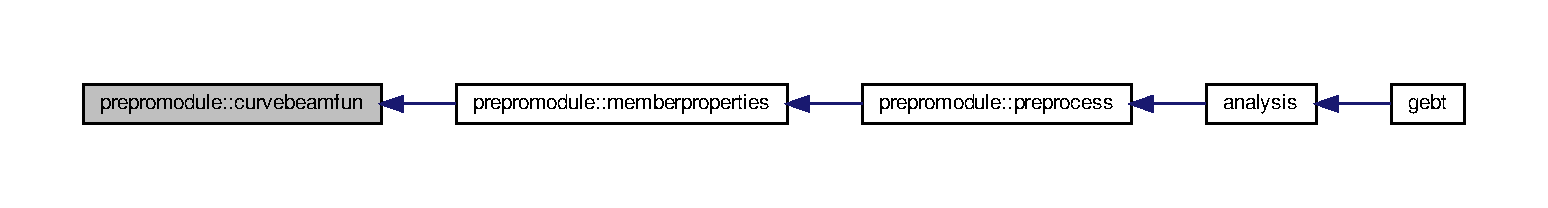
\includegraphics[width=350pt]{namespaceprepromodule_aba8b0787c8f7aa138ead8a8c9161bc4b_icgraph}
\end{center}
\end{figure}
\mbox{\Hypertarget{namespaceprepromodule_a2011e4ceff94f407d454a10cc186d45b}\label{namespaceprepromodule_a2011e4ceff94f407d454a10cc186d45b}} 
\index{prepromodule@{prepromodule}!memberproperties@{memberproperties}}
\index{memberproperties@{memberproperties}!prepromodule@{prepromodule}}
\subsubsection{\texorpdfstring{memberproperties()}{memberproperties()}}
{\footnotesize\ttfamily subroutine prepromodule\+::memberproperties (\begin{DoxyParamCaption}\item[{integer, intent(in)}]{memb\+\_\+no,  }\item[{integer, intent(in)}]{ndof\+\_\+el,  }\item[{integer, dimension(\+:,\+:), intent(in)}]{member,  }\item[{real(dbl), dimension(\+:,\+:,\+:), intent(in)}]{material,  }\item[{real(dbl), dimension(\+:,\+:,\+:), intent(in)}]{frame,  }\item[{real(dbl), dimension(\+:,\+:), intent(in)}]{coord,  }\item[{real(dbl), dimension(\+:,\+:), intent(in)}]{curvature,  }\item[{type (memberinf), intent(out)}]{memb\+\_\+info\+\_\+i,  }\item[{character($\ast$), intent(out)}]{error,  }\item[{integer, intent(in)}]{aero\+\_\+flag,  }\item[{integer, intent(in)}]{grav\+\_\+flag,  }\item[{real(dbl), dimension(\+:,\+:), intent(in), optional}]{aerodyn\+\_\+coef }\end{DoxyParamCaption})\hspace{0.3cm}{\ttfamily [private]}}



Extract member properties for each division $\ast$. 


\begin{DoxyParams}[1]{Parameters}
\mbox{\tt in}  & {\em memb\+\_\+no} & member index\\
\hline
\mbox{\tt in}  & {\em ndof\+\_\+el} & \hyperlink{namespaceioaero_a2b095b5cb5aab1f100d202c8004c9cb5}{ioaero\+::ndof\+\_\+el}\\
\hline
\mbox{\tt in}  & {\em member} & \hyperlink{namespaceioaero_ae040b39fe109c45b001985415e230ec3}{ioaero\+::member}\\
\hline
\mbox{\tt in}  & {\em aero\+\_\+flag} & \hyperlink{namespaceioaero_afb280b6ca8de323c9a07076df81a71e1}{ioaero\+::aero\+\_\+flag}\\
\hline
\mbox{\tt in}  & {\em grav\+\_\+flag} & \hyperlink{namespaceioaero_a831fe87d45ef05e3e29a8c4c2fc88c8f}{ioaero\+::grav\+\_\+flag}\\
\hline
\mbox{\tt in}  & {\em material} & \hyperlink{namespaceioaero_a83ca534029c39300d045045432607a69}{ioaero\+::material}\\
\hline
\mbox{\tt in}  & {\em frame} & \hyperlink{namespaceioaero_a26d467b1adbb838f4b1ba3dd4ee1ea0d}{ioaero\+::frame}\\
\hline
\mbox{\tt in}  & {\em coord} & \hyperlink{namespaceioaero_ad67cddc00712c4d5a6d4008b2fe6c452}{ioaero\+::coord}\\
\hline
\mbox{\tt in}  & {\em curvature} & \hyperlink{namespaceioaero_ab2bc17b64328528015d161cab6490b80}{ioaero\+::curvature}\\
\hline
\mbox{\tt in}  & {\em aerodyn\+\_\+coef} & \hyperlink{namespaceioaero_a116b30aa43f6d871e7d4a3ed6f4428c3}{ioaero\+::aerodyn\+\_\+coef}\\
\hline
\mbox{\tt out}  & {\em memb\+\_\+info\+\_\+i} & the characteristics of the ith beam member\\
\hline
\mbox{\tt out}  & {\em error} & \hyperlink{namespaceioaero_aebd85ae2a176f49a7213d8ed7b68f887}{ioaero\+::error} \\
\hline
\end{DoxyParams}


Definition at line 188 of file Preprocess.\+f90.

Here is the caller graph for this function\+:\nopagebreak
\begin{figure}[H]
\begin{center}
\leavevmode
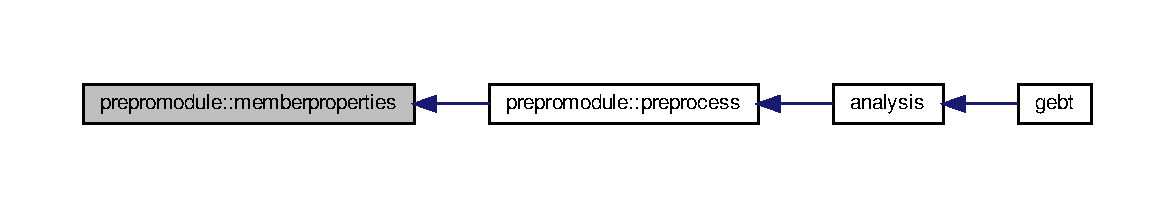
\includegraphics[width=350pt]{namespaceprepromodule_a2011e4ceff94f407d454a10cc186d45b_icgraph}
\end{center}
\end{figure}
\mbox{\Hypertarget{namespaceprepromodule_a4c7a91f217e227051ae54c12a67e702e}\label{namespaceprepromodule_a4c7a91f217e227051ae54c12a67e702e}} 
\index{prepromodule@{prepromodule}!preprocess@{preprocess}}
\index{preprocess@{preprocess}!prepromodule@{prepromodule}}
\subsubsection{\texorpdfstring{preprocess()}{preprocess()}}
{\footnotesize\ttfamily subroutine, public prepromodule\+::preprocess (\begin{DoxyParamCaption}\item[{integer, intent(in)}]{nkp,  }\item[{integer, intent(in)}]{nelem,  }\item[{integer, intent(in)}]{ndof\+\_\+el,  }\item[{integer, dimension(\+:,\+:), intent(in)}]{member,  }\item[{real(dbl), dimension(\+:,\+:,\+:), intent(inout)}]{material,  }\item[{real(dbl), dimension(\+:,\+:,\+:), intent(in)}]{frame,  }\item[{real(dbl), dimension(\+:,\+:), intent(in)}]{coord,  }\item[{real(dbl), dimension(\+:,\+:), intent(in)}]{curvature,  }\item[{integer, dimension(\+:), intent(out)}]{dof\+\_\+con,  }\item[{type (memberinf), dimension(\+:), intent(out)}]{memb\+\_\+info,  }\item[{character($\ast$), intent(out)}]{error,  }\item[{integer, intent(in)}]{aero\+\_\+flag,  }\item[{integer, intent(in)}]{grav\+\_\+flag,  }\item[{real(dbl), dimension(\+:,\+:), intent(in), optional}]{aerodyn\+\_\+coef }\end{DoxyParamCaption})}



Obtaining the connection condition for each key point $\ast$ if a point is connected to more than one member, it is $\ast$ a connection point, otherwise it is a boundary point. $\ast$ It also calculates the size of the problem $\ast$. 


\begin{DoxyParams}[1]{Parameters}
\mbox{\tt in}  & {\em nkp} & \hyperlink{namespaceioaero_a24506866304c39bd1fa57ef73b124335}{ioaero\+::nkp}\\
\hline
\mbox{\tt in}  & {\em nelem} & \hyperlink{namespaceioaero_a543ebf3623a96606d0956211621ce254}{ioaero\+::nelem}\\
\hline
\mbox{\tt in}  & {\em aero\+\_\+flag} & \hyperlink{namespaceioaero_afb280b6ca8de323c9a07076df81a71e1}{ioaero\+::aero\+\_\+flag}\\
\hline
\mbox{\tt in}  & {\em grav\+\_\+flag} & \hyperlink{namespaceioaero_a831fe87d45ef05e3e29a8c4c2fc88c8f}{ioaero\+::grav\+\_\+flag}\\
\hline
\mbox{\tt in}  & {\em ndof\+\_\+el} & \hyperlink{namespaceioaero_a2b095b5cb5aab1f100d202c8004c9cb5}{ioaero\+::ndof\+\_\+el}\\
\hline
\mbox{\tt in}  & {\em member} & \hyperlink{namespaceioaero_ae040b39fe109c45b001985415e230ec3}{ioaero\+::member}\\
\hline
\mbox{\tt in,out}  & {\em material} & \hyperlink{namespaceioaero_a83ca534029c39300d045045432607a69}{ioaero\+::material}\\
\hline
\mbox{\tt in}  & {\em frame} & \hyperlink{namespaceioaero_a26d467b1adbb838f4b1ba3dd4ee1ea0d}{ioaero\+::frame}\\
\hline
\mbox{\tt in}  & {\em coord} & \hyperlink{namespaceioaero_ad67cddc00712c4d5a6d4008b2fe6c452}{ioaero\+::coord}\\
\hline
\mbox{\tt in}  & {\em curvature} & \hyperlink{namespaceioaero_ab2bc17b64328528015d161cab6490b80}{ioaero\+::curvature}\\
\hline
\mbox{\tt in}  & {\em aerodyn\+\_\+coef} & \hyperlink{namespaceioaero_a116b30aa43f6d871e7d4a3ed6f4428c3}{ioaero\+::aerodyn\+\_\+coef}\\
\hline
\mbox{\tt out}  & {\em dof\+\_\+con} & the connecting condition for key point.\\
\hline
\mbox{\tt out}  & {\em memb\+\_\+info} & the member parameters of the whole structure \\
\hline
\end{DoxyParams}


Definition at line 43 of file Preprocess.\+f90.

Here is the caller graph for this function\+:\nopagebreak
\begin{figure}[H]
\begin{center}
\leavevmode
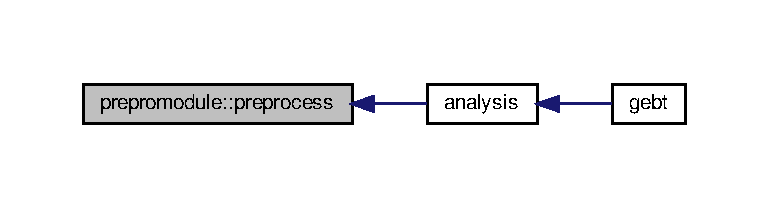
\includegraphics[width=350pt]{namespaceprepromodule_a4c7a91f217e227051ae54c12a67e702e_icgraph}
\end{center}
\end{figure}
\mbox{\Hypertarget{namespaceprepromodule_a078487e47a4a49a0b7f7c94be9f2c8f9}\label{namespaceprepromodule_a078487e47a4a49a0b7f7c94be9f2c8f9}} 
\index{prepromodule@{prepromodule}!rtbis@{rtbis}}
\index{rtbis@{rtbis}!prepromodule@{prepromodule}}
\subsubsection{\texorpdfstring{rtbis()}{rtbis()}}
{\footnotesize\ttfamily real(dbl) function prepromodule\+::rtbis (\begin{DoxyParamCaption}\item[{}]{func,  }\item[{real(dbl), intent(in)}]{kn,  }\item[{real(dbl), intent(in)}]{mL,  }\item[{real(dbl), intent(in)}]{kn2,  }\item[{real(dbl), intent(in)}]{k12,  }\item[{real(dbl), intent(in)}]{kn4,  }\item[{real(dbl), intent(in)}]{x1,  }\item[{real(dbl), intent(in)}]{x2,  }\item[{real(dbl), intent(in)}]{xacc,  }\item[{integer, intent(in)}]{maxit,  }\item[{character($\ast$), intent(out)}]{error }\end{DoxyParamCaption})\hspace{0.3cm}{\ttfamily [private]}}



Use biosection to find root of a function $\ast$ from the book of Numerical Recipes $\ast$. 



Definition at line 368 of file Preprocess.\+f90.

Here is the caller graph for this function\+:\nopagebreak
\begin{figure}[H]
\begin{center}
\leavevmode
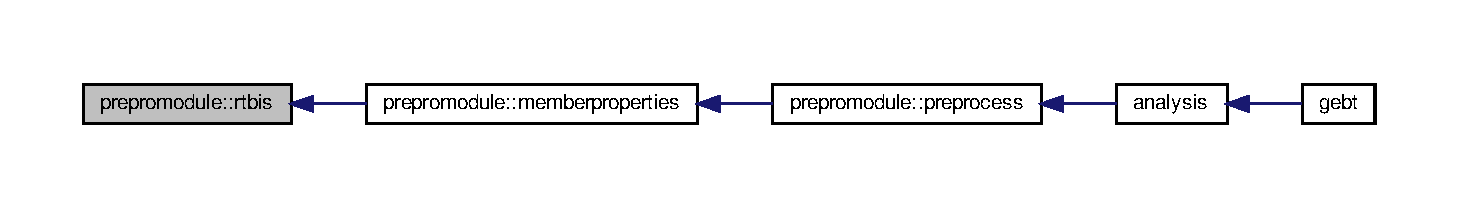
\includegraphics[width=350pt]{namespaceprepromodule_a078487e47a4a49a0b7f7c94be9f2c8f9_icgraph}
\end{center}
\end{figure}


\subsection{Variable Documentation}
\mbox{\Hypertarget{namespaceprepromodule_a41d66ef3ffc050f01bc1763c62c6f3e1}\label{namespaceprepromodule_a41d66ef3ffc050f01bc1763c62c6f3e1}} 
\index{prepromodule@{prepromodule}!ncol\+\_\+memb@{ncol\+\_\+memb}}
\index{ncol\+\_\+memb@{ncol\+\_\+memb}!prepromodule@{prepromodule}}
\subsubsection{\texorpdfstring{ncol\+\_\+memb}{ncol\_memb}}
{\footnotesize\ttfamily integer prepromodule\+::ncol\+\_\+memb\hspace{0.3cm}{\ttfamily [private]}}



\hyperlink{namespacemember_a20895477b227a3352a4e758b21b01bf8}{member\+::ncol\+\_\+memb} 



Definition at line 28 of file Preprocess.\+f90.

\mbox{\Hypertarget{namespaceprepromodule_a6339275501f8c1e8f0b418c9e918005e}\label{namespaceprepromodule_a6339275501f8c1e8f0b418c9e918005e}} 
\index{prepromodule@{prepromodule}!ndiv@{ndiv}}
\index{ndiv@{ndiv}!prepromodule@{prepromodule}}
\subsubsection{\texorpdfstring{ndiv}{ndiv}}
{\footnotesize\ttfamily integer prepromodule\+::ndiv\hspace{0.3cm}{\ttfamily [private]}}



\hyperlink{namespacemember_a3e6a3b0896edb5c30c113dc22ab7181a}{member\+::ndiv} 



Definition at line 27 of file Preprocess.\+f90.


\hypertarget{namespaceprescribedcondition}{}\section{prescribedcondition Module Reference}
\label{namespaceprescribedcondition}\index{prescribedcondition@{prescribedcondition}}


A module for defining prescribed conditions including both concentrated information and distributed information.  


\subsection*{Data Types}
\begin{DoxyCompactItemize}
\item 
type \hyperlink{structprescribedcondition_1_1distriload}{distriload}
\begin{DoxyCompactList}\small\item\em Define the distributed load condition. \end{DoxyCompactList}\item 
type \hyperlink{structprescribedcondition_1_1prescriinf}{prescriinf}
\begin{DoxyCompactList}\small\item\em Define the prescribed condition. \end{DoxyCompactList}\end{DoxyCompactItemize}
\subsection*{Functions/\+Subroutines}
\begin{DoxyCompactItemize}
\item 
subroutine, public \hyperlink{namespaceprescribedcondition_acb722f1fdcfebc72bc33fb3162d9db6d}{existpi} (location, prescri\+\_\+inf, exist\+\_\+pi, follower\+\_\+pi)
\begin{DoxyCompactList}\small\item\em Determine whether prescribed condition exist, and whether any of such conditions is a follower condition. \end{DoxyCompactList}\item 
type(\hyperlink{structprescribedcondition_1_1distriload}{distriload}) function, public \hyperlink{namespaceprescribedcondition_a3f553c3c92903ed635511b07840774ff}{getdistributedload} (memb\+\_\+no, mb\+\_\+condition, distr\+\_\+fun)
\begin{DoxyCompactList}\small\item\em Obtain the distributed load condition. \end{DoxyCompactList}\item 
real(dbl) function, dimension(nstrn), public \hyperlink{namespaceprescribedcondition_a6f624d814d4a2927fd9cc778231e6840}{getload} (flag, dL, Le, e\+CT, load, follower\+\_\+load)
\begin{DoxyCompactList}\small\item\em Obtain the distributed load, transform if follower. \end{DoxyCompactList}\item 
real(dbl) function, dimension(nstrn, 3), public \hyperlink{namespaceprescribedcondition_aa1915c03ae6332a4fa577bcbc8ca2a68}{getloadj} (flag, dL, Le, e\+C\+Ttheta, load)
\begin{DoxyCompactList}\small\item\em Obtain the jacobian due to follower distributed load $\ast$. \end{DoxyCompactList}\item 
subroutine, public \hyperlink{namespaceprescribedcondition_a88f45dfc44f37db180ed595e112a2a36}{getprescribeddof} (nkp, pt\+\_\+condition, kp\+\_\+dof, kp\+\_\+follower)
\begin{DoxyCompactList}\small\item\em Obtain Prescribed dof and follower condition $\ast$. \end{DoxyCompactList}\item 
subroutine, public \hyperlink{namespaceprescribedcondition_aca74e9a71af6abd13879e147076e89ef}{getprescribedval} (nkp, pt\+\_\+condition, kp\+\_\+cond)
\begin{DoxyCompactList}\small\item\em Obtain Prescribed value $\ast$. \end{DoxyCompactList}\item 
elemental type(\hyperlink{structprescribedcondition_1_1prescriinf}{prescriinf}) function, public \hyperlink{namespaceprescribedcondition_ae3bccf07eaf4452047a11ce8dcb3e554}{initpi} ()
\begin{DoxyCompactList}\small\item\em Initialize Prescribed Conditions $\ast$. \end{DoxyCompactList}\item 
type(\hyperlink{structprescribedcondition_1_1prescriinf}{prescriinf}) function, public \hyperlink{namespaceprescribedcondition_a66d378b405e124a0d9a7ad04e262109b}{inputechoprescribedconditions} (IN, E\+IN, error)
\begin{DoxyCompactList}\small\item\em Input and echo Prescribed Conditions $\ast$. \end{DoxyCompactList}\item 
real(dbl) function, dimension(nstrn), public \hyperlink{namespaceprescribedcondition_a58a4332d8bb0ceb882aa3229085dce34}{updatefollower} (kp\+\_\+dof, kp\+\_\+follower, kp\+\_\+cond, x\+\_\+pt)
\begin{DoxyCompactList}\small\item\em Obtain Prescribed D\+OF and value needed for rhs assume only follower force/moments, and no displacements or rotations can be prescribed for follower quantities. And the first three prescribed dofs for the point with a follower component should be either 7 8 9 or 10 11 12. This assumption is made for the easiness to locate the rotation parameters. \end{DoxyCompactList}\item 
subroutine, public \hyperlink{namespaceprescribedcondition_a270714d4f42553a8f966674392dedbfe}{updatepi} (prescri\+\_\+inf, time\+\_\+fun, t)
\begin{DoxyCompactList}\small\item\em Update the prescribed information based on the current time the value is stored in\+: value\+\_\+current. \end{DoxyCompactList}\item 
real(dbl) function, dimension(size(vec), size(vec)), public \hyperlink{namespaceprescribedcondition_a4c109cd4a8df6fedff99e15f448cf944}{followerj} (follower, vec, e\+C\+Ttheta)
\begin{DoxyCompactList}\small\item\em Calculating the Jacobian due to follower conditions $ J=diff{C^T.vec}/diff\theta $, return a 3x3 matrix with ith column corresponding to the derivative withe respect to $ \theta_i $. \end{DoxyCompactList}\item 
real(dbl) function \hyperlink{namespaceprescribedcondition_a55980eb8579eed448879c6118e6218c7}{loadintegration} (flag, dL, Le, func)
\begin{DoxyCompactList}\small\item\em Caculate the load using Chebychev polynomials $\ast$. \end{DoxyCompactList}\item 
real(dbl) function, dimension(size(vec)) \hyperlink{namespaceprescribedcondition_aa60c7ca2dee406dc7cda895535b36927}{transferfollower} (follower, vec, CT)
\begin{DoxyCompactList}\small\item\em Transfer follower according to C$^\wedge$T.vec note vec is a 3x1 vector, and whether a component is a follower or not is determined by follower. \end{DoxyCompactList}\item 
elemental type(\hyperlink{structprescribedcondition_1_1prescriinf}{prescriinf}) function, public \hyperlink{namespaceprescribedcondition_a29eb27f666876bff8a4577eb21d5b2d1}{initpiaero} (i)
\end{DoxyCompactItemize}


\subsection{Detailed Description}
A module for defining prescribed conditions including both concentrated information and distributed information. 

\subsection{Function/\+Subroutine Documentation}
\mbox{\Hypertarget{namespaceprescribedcondition_acb722f1fdcfebc72bc33fb3162d9db6d}\label{namespaceprescribedcondition_acb722f1fdcfebc72bc33fb3162d9db6d}} 
\index{prescribedcondition@{prescribedcondition}!existpi@{existpi}}
\index{existpi@{existpi}!prescribedcondition@{prescribedcondition}}
\subsubsection{\texorpdfstring{existpi()}{existpi()}}
{\footnotesize\ttfamily subroutine, public prescribedcondition\+::existpi (\begin{DoxyParamCaption}\item[{integer, intent(in)}]{location,  }\item[{type(\hyperlink{structprescribedcondition_1_1prescriinf}{prescriinf}), dimension(\+:), intent(in)}]{prescri\+\_\+inf,  }\item[{logical, intent(out)}]{exist\+\_\+pi,  }\item[{logical, intent(out)}]{follower\+\_\+pi }\end{DoxyParamCaption})}



Determine whether prescribed condition exist, and whether any of such conditions is a follower condition. 



Definition at line 59 of file Prescribed\+Condition.\+f90.

\mbox{\Hypertarget{namespaceprescribedcondition_a4c109cd4a8df6fedff99e15f448cf944}\label{namespaceprescribedcondition_a4c109cd4a8df6fedff99e15f448cf944}} 
\index{prescribedcondition@{prescribedcondition}!followerj@{followerj}}
\index{followerj@{followerj}!prescribedcondition@{prescribedcondition}}
\subsubsection{\texorpdfstring{followerj()}{followerj()}}
{\footnotesize\ttfamily real(dbl) function, dimension(size(vec),size(vec)), public prescribedcondition\+::followerj (\begin{DoxyParamCaption}\item[{integer, dimension(\+:), intent(in)}]{follower,  }\item[{real(dbl), dimension(\+:), intent(in)}]{vec,  }\item[{real(dbl), dimension(\+:,\+:,\+:), intent(in)}]{e\+C\+Ttheta }\end{DoxyParamCaption})}



Calculating the Jacobian due to follower conditions $ J=diff{C^T.vec}/diff\theta $, return a 3x3 matrix with ith column corresponding to the derivative withe respect to $ \theta_i $. 



Definition at line 385 of file Prescribed\+Condition.\+f90.

\mbox{\Hypertarget{namespaceprescribedcondition_a3f553c3c92903ed635511b07840774ff}\label{namespaceprescribedcondition_a3f553c3c92903ed635511b07840774ff}} 
\index{prescribedcondition@{prescribedcondition}!getdistributedload@{getdistributedload}}
\index{getdistributedload@{getdistributedload}!prescribedcondition@{prescribedcondition}}
\subsubsection{\texorpdfstring{getdistributedload()}{getdistributedload()}}
{\footnotesize\ttfamily type(\hyperlink{structprescribedcondition_1_1distriload}{distriload}) function, public prescribedcondition\+::getdistributedload (\begin{DoxyParamCaption}\item[{integer, intent(in)}]{memb\+\_\+no,  }\item[{type(\hyperlink{structprescribedcondition_1_1prescriinf}{prescriinf}), dimension(\+:), intent(in)}]{mb\+\_\+condition,  }\item[{real(dbl), dimension(\+:,\+:), intent(in)}]{distr\+\_\+fun }\end{DoxyParamCaption})}



Obtain the distributed load condition. 


\begin{DoxyParams}[1]{Parameters}
\mbox{\tt in}  & {\em memb\+\_\+no} & index of the beam member\\
\hline
\mbox{\tt in}  & {\em distr\+\_\+fun} & \hyperlink{namespaceioaero_a1d7c3689e30c2925cd403a84e9176242}{ioaero\+::distr\+\_\+fun}\\
\hline
\mbox{\tt in}  & {\em mb\+\_\+condition} & distributed load information \\
\hline
\end{DoxyParams}


Definition at line 83 of file Prescribed\+Condition.\+f90.

\mbox{\Hypertarget{namespaceprescribedcondition_a6f624d814d4a2927fd9cc778231e6840}\label{namespaceprescribedcondition_a6f624d814d4a2927fd9cc778231e6840}} 
\index{prescribedcondition@{prescribedcondition}!getload@{getload}}
\index{getload@{getload}!prescribedcondition@{prescribedcondition}}
\subsubsection{\texorpdfstring{getload()}{getload()}}
{\footnotesize\ttfamily real(dbl) function, dimension(nstrn), public prescribedcondition\+::getload (\begin{DoxyParamCaption}\item[{integer, intent(in)}]{flag,  }\item[{real(dbl), intent(in)}]{dL,  }\item[{real(dbl), intent(in)}]{Le,  }\item[{real(dbl), dimension(\+:,\+:), intent(in)}]{e\+CT,  }\item[{type (\hyperlink{structprescribedcondition_1_1distriload}{distriload}), intent(in)}]{load,  }\item[{logical, intent(in)}]{follower\+\_\+load }\end{DoxyParamCaption})}



Obtain the distributed load, transform if follower. 


\begin{DoxyParams}[1]{Parameters}
\mbox{\tt in}  & {\em flag} & if flag=-\/1, the starting portion, if flag=1, the ending portion \\
\hline
\end{DoxyParams}


Definition at line 116 of file Prescribed\+Condition.\+f90.

\mbox{\Hypertarget{namespaceprescribedcondition_aa1915c03ae6332a4fa577bcbc8ca2a68}\label{namespaceprescribedcondition_aa1915c03ae6332a4fa577bcbc8ca2a68}} 
\index{prescribedcondition@{prescribedcondition}!getloadj@{getloadj}}
\index{getloadj@{getloadj}!prescribedcondition@{prescribedcondition}}
\subsubsection{\texorpdfstring{getloadj()}{getloadj()}}
{\footnotesize\ttfamily real(dbl) function, dimension(nstrn,3), public prescribedcondition\+::getloadj (\begin{DoxyParamCaption}\item[{integer, intent(in)}]{flag,  }\item[{real(dbl), intent(in)}]{dL,  }\item[{real(dbl), intent(in)}]{Le,  }\item[{real(dbl), dimension(\+:,\+:,\+:), intent(in)}]{e\+C\+Ttheta,  }\item[{type (\hyperlink{structprescribedcondition_1_1distriload}{distriload}), intent(in)}]{load }\end{DoxyParamCaption})}



Obtain the jacobian due to follower distributed load $\ast$. 



Definition at line 149 of file Prescribed\+Condition.\+f90.

\mbox{\Hypertarget{namespaceprescribedcondition_a88f45dfc44f37db180ed595e112a2a36}\label{namespaceprescribedcondition_a88f45dfc44f37db180ed595e112a2a36}} 
\index{prescribedcondition@{prescribedcondition}!getprescribeddof@{getprescribeddof}}
\index{getprescribeddof@{getprescribeddof}!prescribedcondition@{prescribedcondition}}
\subsubsection{\texorpdfstring{getprescribeddof()}{getprescribeddof()}}
{\footnotesize\ttfamily subroutine, public prescribedcondition\+::getprescribeddof (\begin{DoxyParamCaption}\item[{integer, intent(in)}]{nkp,  }\item[{type(\hyperlink{structprescribedcondition_1_1prescriinf}{prescriinf}), dimension(\+:), intent(in)}]{pt\+\_\+condition,  }\item[{integer, dimension(\+:,\+:), intent(out)}]{kp\+\_\+dof,  }\item[{integer, dimension(\+:,\+:), intent(out)}]{kp\+\_\+follower }\end{DoxyParamCaption})}



Obtain Prescribed dof and follower condition $\ast$. 


\begin{DoxyParams}[1]{Parameters}
\mbox{\tt in}  & {\em nkp} & \hyperlink{namespaceioaero_a24506866304c39bd1fa57ef73b124335}{ioaero\+::nkp} \\
\hline
\end{DoxyParams}


Definition at line 183 of file Prescribed\+Condition.\+f90.

\mbox{\Hypertarget{namespaceprescribedcondition_aca74e9a71af6abd13879e147076e89ef}\label{namespaceprescribedcondition_aca74e9a71af6abd13879e147076e89ef}} 
\index{prescribedcondition@{prescribedcondition}!getprescribedval@{getprescribedval}}
\index{getprescribedval@{getprescribedval}!prescribedcondition@{prescribedcondition}}
\subsubsection{\texorpdfstring{getprescribedval()}{getprescribedval()}}
{\footnotesize\ttfamily subroutine, public prescribedcondition\+::getprescribedval (\begin{DoxyParamCaption}\item[{integer, intent(in)}]{nkp,  }\item[{type(\hyperlink{structprescribedcondition_1_1prescriinf}{prescriinf}), dimension(\+:), intent(in)}]{pt\+\_\+condition,  }\item[{real(dbl), dimension(\+:,\+:), intent(out)}]{kp\+\_\+cond }\end{DoxyParamCaption})}



Obtain Prescribed value $\ast$. 


\begin{DoxyParams}[1]{Parameters}
\mbox{\tt in}  & {\em nkp} & \hyperlink{namespaceioaero_a24506866304c39bd1fa57ef73b124335}{ioaero\+::nkp}\\
\hline
\mbox{\tt in}  & {\em pt\+\_\+condition} & \hyperlink{namespaceioaero_a4344b2018135ae7fe0a09f4265fd2c29}{ioaero\+::pt\+\_\+condition} \\
\hline
\end{DoxyParams}


Definition at line 212 of file Prescribed\+Condition.\+f90.

\mbox{\Hypertarget{namespaceprescribedcondition_ae3bccf07eaf4452047a11ce8dcb3e554}\label{namespaceprescribedcondition_ae3bccf07eaf4452047a11ce8dcb3e554}} 
\index{prescribedcondition@{prescribedcondition}!initpi@{initpi}}
\index{initpi@{initpi}!prescribedcondition@{prescribedcondition}}
\subsubsection{\texorpdfstring{initpi()}{initpi()}}
{\footnotesize\ttfamily elemental type (\hyperlink{structprescribedcondition_1_1prescriinf}{prescriinf}) function, public prescribedcondition\+::initpi (\begin{DoxyParamCaption}{ }\end{DoxyParamCaption})}



Initialize Prescribed Conditions $\ast$. 



Definition at line 237 of file Prescribed\+Condition.\+f90.

\mbox{\Hypertarget{namespaceprescribedcondition_a29eb27f666876bff8a4577eb21d5b2d1}\label{namespaceprescribedcondition_a29eb27f666876bff8a4577eb21d5b2d1}} 
\index{prescribedcondition@{prescribedcondition}!initpiaero@{initpiaero}}
\index{initpiaero@{initpiaero}!prescribedcondition@{prescribedcondition}}
\subsubsection{\texorpdfstring{initpiaero()}{initpiaero()}}
{\footnotesize\ttfamily elemental type (\hyperlink{structprescribedcondition_1_1prescriinf}{prescriinf}) function, public prescribedcondition\+::initpiaero (\begin{DoxyParamCaption}\item[{integer, intent(in)}]{i }\end{DoxyParamCaption})}



Definition at line 494 of file Prescribed\+Condition.\+f90.

\mbox{\Hypertarget{namespaceprescribedcondition_a66d378b405e124a0d9a7ad04e262109b}\label{namespaceprescribedcondition_a66d378b405e124a0d9a7ad04e262109b}} 
\index{prescribedcondition@{prescribedcondition}!inputechoprescribedconditions@{inputechoprescribedconditions}}
\index{inputechoprescribedconditions@{inputechoprescribedconditions}!prescribedcondition@{prescribedcondition}}
\subsubsection{\texorpdfstring{inputechoprescribedconditions()}{inputechoprescribedconditions()}}
{\footnotesize\ttfamily type (\hyperlink{structprescribedcondition_1_1prescriinf}{prescriinf}) function, public prescribedcondition\+::inputechoprescribedconditions (\begin{DoxyParamCaption}\item[{integer, intent(in)}]{IN,  }\item[{integer, intent(in)}]{E\+IN,  }\item[{character($\ast$), intent(out)}]{error }\end{DoxyParamCaption})}



Input and echo Prescribed Conditions $\ast$. 



Definition at line 258 of file Prescribed\+Condition.\+f90.

\mbox{\Hypertarget{namespaceprescribedcondition_a55980eb8579eed448879c6118e6218c7}\label{namespaceprescribedcondition_a55980eb8579eed448879c6118e6218c7}} 
\index{prescribedcondition@{prescribedcondition}!loadintegration@{loadintegration}}
\index{loadintegration@{loadintegration}!prescribedcondition@{prescribedcondition}}
\subsubsection{\texorpdfstring{loadintegration()}{loadintegration()}}
{\footnotesize\ttfamily real(dbl) function prescribedcondition\+::loadintegration (\begin{DoxyParamCaption}\item[{integer, intent(in)}]{flag,  }\item[{real(dbl), intent(in)}]{dL,  }\item[{real(dbl), intent(in)}]{Le,  }\item[{real(dbl), dimension(nstrn), intent(in)}]{func }\end{DoxyParamCaption})\hspace{0.3cm}{\ttfamily [private]}}



Caculate the load using Chebychev polynomials $\ast$. 


\begin{DoxyParams}[1]{Parameters}
\mbox{\tt in}  & {\em flag} & if flag=-\/1, it is for the starting point, if flag=1, it is for the ending point\\
\hline
\mbox{\tt in}  & {\em dl} & length of the element\\
\hline
\mbox{\tt in}  & {\em le} & the ending point of the element at the arc length of the member\\
\hline
\mbox{\tt in}  & {\em func} & distributed load function for this element\\
\hline
\end{DoxyParams}
\begin{DoxyReturn}{Returns}
the load for each element 
\end{DoxyReturn}


Definition at line 413 of file Prescribed\+Condition.\+f90.

\mbox{\Hypertarget{namespaceprescribedcondition_aa60c7ca2dee406dc7cda895535b36927}\label{namespaceprescribedcondition_aa60c7ca2dee406dc7cda895535b36927}} 
\index{prescribedcondition@{prescribedcondition}!transferfollower@{transferfollower}}
\index{transferfollower@{transferfollower}!prescribedcondition@{prescribedcondition}}
\subsubsection{\texorpdfstring{transferfollower()}{transferfollower()}}
{\footnotesize\ttfamily real(dbl) function, dimension(size(vec)) prescribedcondition\+::transferfollower (\begin{DoxyParamCaption}\item[{integer, dimension(\+:), intent(in)}]{follower,  }\item[{real(dbl), dimension(\+:), intent(in)}]{vec,  }\item[{real(dbl), dimension(\+:,\+:), intent(in)}]{CT }\end{DoxyParamCaption})\hspace{0.3cm}{\ttfamily [private]}}



Transfer follower according to C$^\wedge$T.vec note vec is a 3x1 vector, and whether a component is a follower or not is determined by follower. 



Definition at line 472 of file Prescribed\+Condition.\+f90.

\mbox{\Hypertarget{namespaceprescribedcondition_a58a4332d8bb0ceb882aa3229085dce34}\label{namespaceprescribedcondition_a58a4332d8bb0ceb882aa3229085dce34}} 
\index{prescribedcondition@{prescribedcondition}!updatefollower@{updatefollower}}
\index{updatefollower@{updatefollower}!prescribedcondition@{prescribedcondition}}
\subsubsection{\texorpdfstring{updatefollower()}{updatefollower()}}
{\footnotesize\ttfamily real(dbl) function, dimension(nstrn), public prescribedcondition\+::updatefollower (\begin{DoxyParamCaption}\item[{integer, dimension(\+:), intent(in)}]{kp\+\_\+dof,  }\item[{integer, dimension(\+:), intent(in)}]{kp\+\_\+follower,  }\item[{real(dbl), dimension(\+:), intent(in)}]{kp\+\_\+cond,  }\item[{real(dbl), dimension(\+:), intent(in)}]{x\+\_\+pt }\end{DoxyParamCaption})}



Obtain Prescribed D\+OF and value needed for rhs assume only follower force/moments, and no displacements or rotations can be prescribed for follower quantities. And the first three prescribed dofs for the point with a follower component should be either 7 8 9 or 10 11 12. This assumption is made for the easiness to locate the rotation parameters. 



Definition at line 309 of file Prescribed\+Condition.\+f90.

\mbox{\Hypertarget{namespaceprescribedcondition_a270714d4f42553a8f966674392dedbfe}\label{namespaceprescribedcondition_a270714d4f42553a8f966674392dedbfe}} 
\index{prescribedcondition@{prescribedcondition}!updatepi@{updatepi}}
\index{updatepi@{updatepi}!prescribedcondition@{prescribedcondition}}
\subsubsection{\texorpdfstring{updatepi()}{updatepi()}}
{\footnotesize\ttfamily subroutine, public prescribedcondition\+::updatepi (\begin{DoxyParamCaption}\item[{type (\hyperlink{structprescribedcondition_1_1prescriinf}{prescriinf}), dimension(\+:), intent(inout)}]{prescri\+\_\+inf,  }\item[{type (timefunction), dimension(\+:), intent(in)}]{time\+\_\+fun,  }\item[{real(dbl), intent(in)}]{t }\end{DoxyParamCaption})}



Update the prescribed information based on the current time the value is stored in\+: value\+\_\+current. 



Definition at line 341 of file Prescribed\+Condition.\+f90.


\hypertarget{namespacesolvemumps}{}\section{solvemumps Module Reference}
\label{namespacesolvemumps}\index{solvemumps@{solvemumps}}


This module contains the linear \& nonlinear solver interfaced with M\+U\+M\+PS direct solver library.  


\subsection*{Functions/\+Subroutines}
\begin{DoxyCompactItemize}
\item 
subroutine, public \hyperlink{namespacesolvemumps_aad7849d30a944c0bd614bf4e103ef494}{linearsolutionmumps} (ndof\+\_\+el, memb\+\_\+info, v\+\_\+root\+\_\+a, omega\+\_\+a, member, error, ncond\+\_\+mb, mb\+\_\+condition, distr\+\_\+fun, dof\+\_\+con, x, aero\+\_\+flag, grav\+\_\+flag, init\+\_\+cond)
\begin{DoxyCompactList}\small\item\em The linear solver is basically the Newton-\/\+Raphson with $\ast$ initial guess equal to zero and only uses one iterations $\ast$. \end{DoxyCompactList}\item 
subroutine, public \hyperlink{namespacesolvemumps_a243ff65847b437ecb22933d782df2db4}{newtonraphsonmumps} (ndof\+\_\+el, memb\+\_\+info, v\+\_\+root\+\_\+a, omega\+\_\+a, member, niter, error, ncond\+\_\+mb, mb\+\_\+condition, distr\+\_\+fun, dof\+\_\+con, x, aero\+\_\+flag, grav\+\_\+flag, init\+\_\+cond)
\begin{DoxyCompactList}\small\item\em Use Newton-\/\+Raphson method to solve the nonlinear system $\ast$. \end{DoxyCompactList}\item 
subroutine, public \hyperlink{namespacesolvemumps_aaa9b81bc0ea43f279abc42c729140761}{extractsolution} (ndof\+\_\+el, member, coord, memb\+\_\+info, x, dof\+\_\+con, sol\+\_\+pt\+\_\+i, sol\+\_\+mb\+\_\+i)
\begin{DoxyCompactList}\small\item\em The subroutine extracts the solution for each key point and each member from the solution vector $\ast$. \end{DoxyCompactList}\item 
subroutine, public \hyperlink{namespacesolvemumps_ae4f9a2e645ae55a030964764cf5b0218}{extractelementvalues} (ndof\+\_\+el, member, x, sol\+\_\+mb\+\_\+i)
\begin{DoxyCompactList}\small\item\em The subroutine extracts elemental values from $\ast$ the solution vector $\ast$. \end{DoxyCompactList}\item 
subroutine, public \hyperlink{namespacesolvemumps_a3c8d285942de4048473a98c26d248fd7}{insertelementvalues} (ndof\+\_\+el, member, x, init\+\_\+cond)
\begin{DoxyCompactList}\small\item\em The subroutine insert the elemental values into the solution vector\+: needed for initial guess for starting time marching\+: replace the first six valumes for each element with given initial conditions $\ast$. \end{DoxyCompactList}\item 
real(dbl) function, dimension(size(sol\+\_\+mb\+\_\+i, 1), 6), public \hyperlink{namespacesolvemumps_a680703eba15a14e08417723cd80080b1}{ctcabph} (niter, member, memb\+\_\+info, sol\+\_\+mb\+\_\+i)
\begin{DoxyCompactList}\small\item\em Transfer the vector PH (linear and angular momenta) form frame B to frame a. \end{DoxyCompactList}\end{DoxyCompactItemize}
\subsection*{Variables}
\begin{DoxyCompactItemize}
\item 
type(dmumps\+\_\+struc) \hyperlink{namespacesolvemumps_ab76b5a7f705b0acb09ebc3ecf7e51f91}{mumps\+\_\+par}
\begin{DoxyCompactList}\small\item\em an array containing the configuration parameters of M\+U\+M\+PS solver \end{DoxyCompactList}\item 
integer \hyperlink{namespacesolvemumps_a5f812a31bb5931d66e5d6bb4c05f4a51}{ierr}
\begin{DoxyCompactList}\small\item\em error code of the M\+U\+M\+PS solver \end{DoxyCompactList}\end{DoxyCompactItemize}


\subsection{Detailed Description}
This module contains the linear \& nonlinear solver interfaced with M\+U\+M\+PS direct solver library. 

\subsection{Function/\+Subroutine Documentation}
\mbox{\Hypertarget{namespacesolvemumps_a680703eba15a14e08417723cd80080b1}\label{namespacesolvemumps_a680703eba15a14e08417723cd80080b1}} 
\index{solvemumps@{solvemumps}!ctcabph@{ctcabph}}
\index{ctcabph@{ctcabph}!solvemumps@{solvemumps}}
\subsubsection{\texorpdfstring{ctcabph()}{ctcabph()}}
{\footnotesize\ttfamily real(dbl) function, dimension(size(sol\+\_\+mb\+\_\+i,1),6), public solvemumps\+::ctcabph (\begin{DoxyParamCaption}\item[{integer, intent(in)}]{niter,  }\item[{integer, dimension(\+:,\+:), intent(in)}]{member,  }\item[{type (memberinf), dimension(\+:), intent(in)}]{memb\+\_\+info,  }\item[{real(dbl), dimension(\+:,\+:), intent(in)}]{sol\+\_\+mb\+\_\+i }\end{DoxyParamCaption})}



Transfer the vector PH (linear and angular momenta) form frame B to frame a. 


\begin{DoxyParams}[1]{Parameters}
\mbox{\tt in}  & {\em niter} & \hyperlink{namespaceioaero_ac008486fd12e0029a1ef77b3ca5e12c3}{ioaero\+::niter}\\
\hline
\mbox{\tt in}  & {\em member} & \hyperlink{namespaceioaero_ae040b39fe109c45b001985415e230ec3}{ioaero\+::member}\\
\hline
\mbox{\tt in}  & {\em sol\+\_\+mb\+\_\+i} & solutions for members for ith step \\
\hline
\end{DoxyParams}


Definition at line 535 of file Solve\+Mumps.\+f90.

Here is the caller graph for this function\+:\nopagebreak
\begin{figure}[H]
\begin{center}
\leavevmode
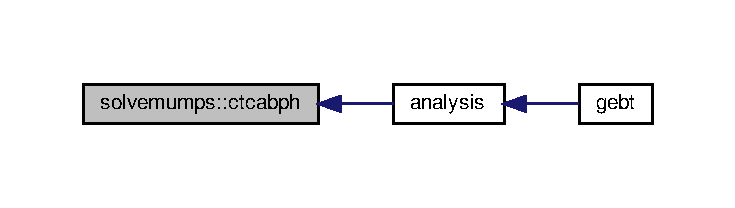
\includegraphics[width=350pt]{namespacesolvemumps_a680703eba15a14e08417723cd80080b1_icgraph}
\end{center}
\end{figure}
\mbox{\Hypertarget{namespacesolvemumps_ae4f9a2e645ae55a030964764cf5b0218}\label{namespacesolvemumps_ae4f9a2e645ae55a030964764cf5b0218}} 
\index{solvemumps@{solvemumps}!extractelementvalues@{extractelementvalues}}
\index{extractelementvalues@{extractelementvalues}!solvemumps@{solvemumps}}
\subsubsection{\texorpdfstring{extractelementvalues()}{extractelementvalues()}}
{\footnotesize\ttfamily subroutine, public solvemumps\+::extractelementvalues (\begin{DoxyParamCaption}\item[{integer, intent(in)}]{ndof\+\_\+el,  }\item[{integer, dimension(\+:,\+:), intent(in)}]{member,  }\item[{real(dbl), dimension(\+:), intent(in)}]{x,  }\item[{real(dbl), dimension(\+:,\+:), intent(out)}]{sol\+\_\+mb\+\_\+i }\end{DoxyParamCaption})}



The subroutine extracts elemental values from $\ast$ the solution vector $\ast$. 


\begin{DoxyParams}[1]{Parameters}
\mbox{\tt in}  & {\em ndof\+\_\+el} & \hyperlink{namespaceioaero_a2b095b5cb5aab1f100d202c8004c9cb5}{ioaero\+::ndof\+\_\+el}\\
\hline
\mbox{\tt in}  & {\em member} & \hyperlink{namespaceioaero_ae040b39fe109c45b001985415e230ec3}{ioaero\+::member}\\
\hline
\mbox{\tt in}  & {\em x} & the solution vector\\
\hline
\mbox{\tt out}  & {\em sol\+\_\+mb\+\_\+i} & solutions for all the elements for ith step \\
\hline
\end{DoxyParams}


Definition at line 464 of file Solve\+Mumps.\+f90.

Here is the caller graph for this function\+:\nopagebreak
\begin{figure}[H]
\begin{center}
\leavevmode
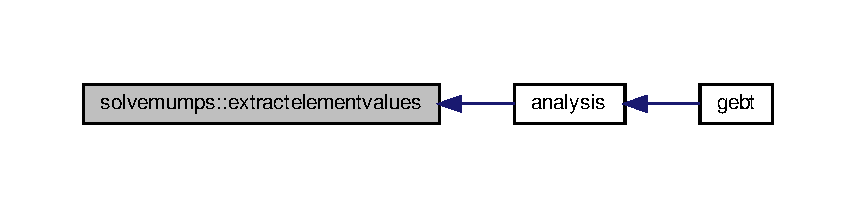
\includegraphics[width=350pt]{namespacesolvemumps_ae4f9a2e645ae55a030964764cf5b0218_icgraph}
\end{center}
\end{figure}
\mbox{\Hypertarget{namespacesolvemumps_aaa9b81bc0ea43f279abc42c729140761}\label{namespacesolvemumps_aaa9b81bc0ea43f279abc42c729140761}} 
\index{solvemumps@{solvemumps}!extractsolution@{extractsolution}}
\index{extractsolution@{extractsolution}!solvemumps@{solvemumps}}
\subsubsection{\texorpdfstring{extractsolution()}{extractsolution()}}
{\footnotesize\ttfamily subroutine, public solvemumps\+::extractsolution (\begin{DoxyParamCaption}\item[{integer, intent(in)}]{ndof\+\_\+el,  }\item[{integer, dimension(\+:,\+:), intent(in)}]{member,  }\item[{real(dbl), dimension(\+:,\+:), intent(in)}]{coord,  }\item[{type (memberinf), dimension(\+:), intent(in)}]{memb\+\_\+info,  }\item[{real(dbl), dimension(\+:), intent(in)}]{x,  }\item[{integer, dimension(\+:), intent(in)}]{dof\+\_\+con,  }\item[{real(dbl), dimension(\+:,\+:), intent(out)}]{sol\+\_\+pt\+\_\+i,  }\item[{real(dbl), dimension(\+:,\+:), intent(out)}]{sol\+\_\+mb\+\_\+i }\end{DoxyParamCaption})}



The subroutine extracts the solution for each key point and each member from the solution vector $\ast$. 


\begin{DoxyParams}[1]{Parameters}
\mbox{\tt in}  & {\em ndof\+\_\+el} & \hyperlink{namespaceioaero_a2b095b5cb5aab1f100d202c8004c9cb5}{ioaero\+::ndof\+\_\+el}\\
\hline
\mbox{\tt in}  & {\em member} & \hyperlink{namespaceioaero_ae040b39fe109c45b001985415e230ec3}{ioaero\+::member}\\
\hline
\mbox{\tt in}  & {\em coord} & \hyperlink{namespaceioaero_ad67cddc00712c4d5a6d4008b2fe6c452}{ioaero\+::coord}\\
\hline
\mbox{\tt in}  & {\em memb\+\_\+info} & contains the member parameters of the whole structure\\
\hline
\mbox{\tt in}  & {\em x} & the solution vector\\
\hline
\mbox{\tt in}  & {\em dof\+\_\+con} & the connecting condition for key point.\\
\hline
\mbox{\tt out}  & {\em sol\+\_\+pt\+\_\+i} & solutions for points for ith step\\
\hline
\mbox{\tt out}  & {\em sol\+\_\+mb\+\_\+i} & solutions for members for ith step \\
\hline
\end{DoxyParams}


Definition at line 384 of file Solve\+Mumps.\+f90.

Here is the caller graph for this function\+:\nopagebreak
\begin{figure}[H]
\begin{center}
\leavevmode
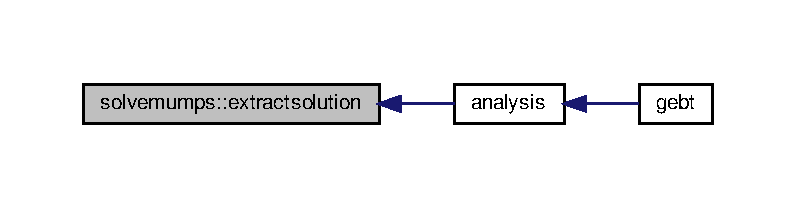
\includegraphics[width=350pt]{namespacesolvemumps_aaa9b81bc0ea43f279abc42c729140761_icgraph}
\end{center}
\end{figure}
\mbox{\Hypertarget{namespacesolvemumps_a3c8d285942de4048473a98c26d248fd7}\label{namespacesolvemumps_a3c8d285942de4048473a98c26d248fd7}} 
\index{solvemumps@{solvemumps}!insertelementvalues@{insertelementvalues}}
\index{insertelementvalues@{insertelementvalues}!solvemumps@{solvemumps}}
\subsubsection{\texorpdfstring{insertelementvalues()}{insertelementvalues()}}
{\footnotesize\ttfamily subroutine, public solvemumps\+::insertelementvalues (\begin{DoxyParamCaption}\item[{integer, intent(in)}]{ndof\+\_\+el,  }\item[{integer, dimension(\+:,\+:), intent(in)}]{member,  }\item[{real(dbl), dimension(\+:), intent(inout)}]{x,  }\item[{real(dbl), dimension(\+:,\+:), intent(in)}]{init\+\_\+cond }\end{DoxyParamCaption})}



The subroutine insert the elemental values into the solution vector\+: needed for initial guess for starting time marching\+: replace the first six valumes for each element with given initial conditions $\ast$. 


\begin{DoxyParams}[1]{Parameters}
\mbox{\tt in}  & {\em ndof\+\_\+el} & \hyperlink{namespaceioaero_a2b095b5cb5aab1f100d202c8004c9cb5}{ioaero\+::ndof\+\_\+el}\\
\hline
\mbox{\tt in}  & {\em member} & \#ioaero\+::memeber\\
\hline
\mbox{\tt in,out}  & {\em x} & the solution vector\\
\hline
\mbox{\tt in}  & {\em init\+\_\+cond} & \hyperlink{namespaceioaero_ad88d83709eb2f4596a89098db11ba770}{ioaero\+::init\+\_\+cond} \\
\hline
\end{DoxyParams}


Definition at line 501 of file Solve\+Mumps.\+f90.

Here is the caller graph for this function\+:\nopagebreak
\begin{figure}[H]
\begin{center}
\leavevmode
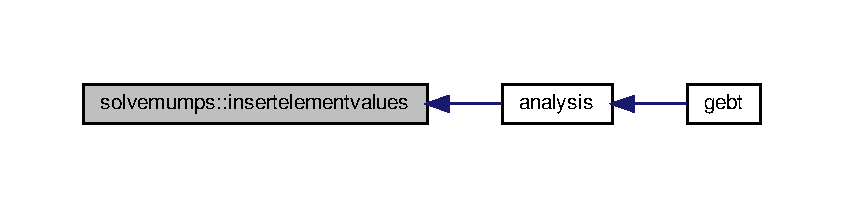
\includegraphics[width=350pt]{namespacesolvemumps_a3c8d285942de4048473a98c26d248fd7_icgraph}
\end{center}
\end{figure}
\mbox{\Hypertarget{namespacesolvemumps_aad7849d30a944c0bd614bf4e103ef494}\label{namespacesolvemumps_aad7849d30a944c0bd614bf4e103ef494}} 
\index{solvemumps@{solvemumps}!linearsolutionmumps@{linearsolutionmumps}}
\index{linearsolutionmumps@{linearsolutionmumps}!solvemumps@{solvemumps}}
\subsubsection{\texorpdfstring{linearsolutionmumps()}{linearsolutionmumps()}}
{\footnotesize\ttfamily subroutine, public solvemumps\+::linearsolutionmumps (\begin{DoxyParamCaption}\item[{integer, intent(in)}]{ndof\+\_\+el,  }\item[{type (memberinf), dimension(\+:), intent(in)}]{memb\+\_\+info,  }\item[{real(dbl), dimension(\+:), intent(in)}]{v\+\_\+root\+\_\+a,  }\item[{real(dbl), dimension(\+:), intent(in)}]{omega\+\_\+a,  }\item[{integer, dimension(\+:,\+:), intent(in)}]{member,  }\item[{character($\ast$), intent(out)}]{error,  }\item[{integer, intent(in)}]{ncond\+\_\+mb,  }\item[{type(prescriinf), dimension(\+:), intent(in)}]{mb\+\_\+condition,  }\item[{real(dbl), dimension(\+:,\+:), intent(in)}]{distr\+\_\+fun,  }\item[{integer, dimension(\+:)}]{dof\+\_\+con,  }\item[{real(dbl), dimension(\+:), intent(out)}]{x,  }\item[{integer, intent(in)}]{aero\+\_\+flag,  }\item[{integer, intent(in)}]{grav\+\_\+flag,  }\item[{real(dbl), dimension(\+:,\+:), intent(in), optional}]{init\+\_\+cond }\end{DoxyParamCaption})}



The linear solver is basically the Newton-\/\+Raphson with $\ast$ initial guess equal to zero and only uses one iterations $\ast$. 


\begin{DoxyParams}[1]{Parameters}
\mbox{\tt in}  & {\em ndof\+\_\+el} & \hyperlink{namespaceioaero_a2b095b5cb5aab1f100d202c8004c9cb5}{ioaero\+::ndof\+\_\+el}\\
\hline
\mbox{\tt in}  & {\em aero\+\_\+flag} & \hyperlink{namespaceioaero_afb280b6ca8de323c9a07076df81a71e1}{ioaero\+::aero\+\_\+flag}\\
\hline
\mbox{\tt in}  & {\em grav\+\_\+flag} & \hyperlink{namespaceioaero_a831fe87d45ef05e3e29a8c4c2fc88c8f}{ioaero\+::grav\+\_\+flag}\\
\hline
\mbox{\tt in}  & {\em v\+\_\+root\+\_\+a} & linear velocity of frame a\\
\hline
\mbox{\tt in}  & {\em omega\+\_\+a} & angular velocity of frame a\\
\hline
\mbox{\tt in}  & {\em distr\+\_\+fun} & \hyperlink{namespaceioaero_a1d7c3689e30c2925cd403a84e9176242}{ioaero\+::distr\+\_\+fun}\\
\hline
\mbox{\tt in}  & {\em member} & \hyperlink{namespaceioaero_ae040b39fe109c45b001985415e230ec3}{ioaero\+::member}\\
\hline
\mbox{\tt in}  & {\em ncond\+\_\+mb} & \hyperlink{namespaceioaero_ab9193f4ff70a22ae5858118fc653f22b}{ioaero\+::ncond\+\_\+mb}\\
\hline
\mbox{\tt in}  & {\em mb\+\_\+condition} & \hyperlink{namespaceioaero_a2463929ef049b49fe7b49011c66cc806}{ioaero\+::mb\+\_\+condition}\\
\hline
 & {\em dof\+\_\+con} & this array is passed by value\\
\hline
\mbox{\tt out}  & {\em error} & \hyperlink{namespaceioaero_aebd85ae2a176f49a7213d8ed7b68f887}{ioaero\+::error}\\
\hline
\mbox{\tt out}  & {\em x} & The solution vector\\
\hline
\mbox{\tt in}  & {\em init\+\_\+cond} & \hyperlink{namespaceioaero_ad88d83709eb2f4596a89098db11ba770}{ioaero\+::init\+\_\+cond} \\
\hline
\end{DoxyParams}


Definition at line 42 of file Solve\+Mumps.\+f90.

Here is the caller graph for this function\+:\nopagebreak
\begin{figure}[H]
\begin{center}
\leavevmode
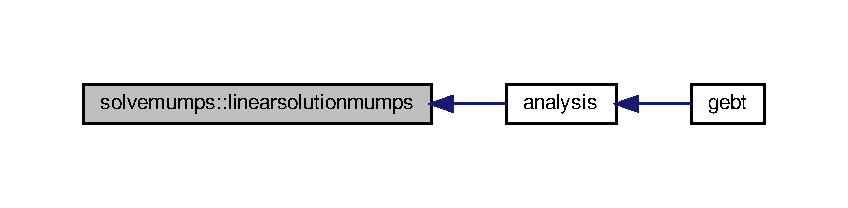
\includegraphics[width=350pt]{namespacesolvemumps_aad7849d30a944c0bd614bf4e103ef494_icgraph}
\end{center}
\end{figure}
\mbox{\Hypertarget{namespacesolvemumps_a243ff65847b437ecb22933d782df2db4}\label{namespacesolvemumps_a243ff65847b437ecb22933d782df2db4}} 
\index{solvemumps@{solvemumps}!newtonraphsonmumps@{newtonraphsonmumps}}
\index{newtonraphsonmumps@{newtonraphsonmumps}!solvemumps@{solvemumps}}
\subsubsection{\texorpdfstring{newtonraphsonmumps()}{newtonraphsonmumps()}}
{\footnotesize\ttfamily subroutine, public solvemumps\+::newtonraphsonmumps (\begin{DoxyParamCaption}\item[{integer, intent(in)}]{ndof\+\_\+el,  }\item[{type (memberinf), dimension(\+:), intent(in)}]{memb\+\_\+info,  }\item[{real(dbl), dimension(\+:), intent(in)}]{v\+\_\+root\+\_\+a,  }\item[{real(dbl), dimension(\+:), intent(in)}]{omega\+\_\+a,  }\item[{integer, dimension(\+:,\+:), intent(in)}]{member,  }\item[{integer, intent(in)}]{niter,  }\item[{character($\ast$), intent(out)}]{error,  }\item[{integer, intent(in)}]{ncond\+\_\+mb,  }\item[{type(prescriinf), dimension(\+:), intent(in)}]{mb\+\_\+condition,  }\item[{real(dbl), dimension(\+:,\+:), intent(in)}]{distr\+\_\+fun,  }\item[{integer, dimension(\+:)}]{dof\+\_\+con,  }\item[{real(dbl), dimension(\+:), intent(inout)}]{x,  }\item[{integer, intent(in)}]{aero\+\_\+flag,  }\item[{integer, intent(in)}]{grav\+\_\+flag,  }\item[{real(dbl), dimension(\+:,\+:), intent(in), optional}]{init\+\_\+cond }\end{DoxyParamCaption})}



Use Newton-\/\+Raphson method to solve the nonlinear system $\ast$. 


\begin{DoxyParams}[1]{Parameters}
\mbox{\tt in}  & {\em ndof\+\_\+el} & \hyperlink{namespaceioaero_a2b095b5cb5aab1f100d202c8004c9cb5}{ioaero\+::ndof\+\_\+el}\\
\hline
\mbox{\tt in}  & {\em aero\+\_\+flag} & \hyperlink{namespaceioaero_afb280b6ca8de323c9a07076df81a71e1}{ioaero\+::aero\+\_\+flag}\\
\hline
\mbox{\tt in}  & {\em grav\+\_\+flag} & \hyperlink{namespaceioaero_a831fe87d45ef05e3e29a8c4c2fc88c8f}{ioaero\+::grav\+\_\+flag}\\
\hline
\mbox{\tt in}  & {\em memb\+\_\+info} & contains the member parameters of the whole structure\\
\hline
\mbox{\tt in}  & {\em v\+\_\+root\+\_\+a} & linear velocity of frame a\\
\hline
\mbox{\tt in}  & {\em omega\+\_\+a} & angular velocity of frame a\\
\hline
\mbox{\tt in}  & {\em distr\+\_\+fun} & \hyperlink{namespaceioaero_a1d7c3689e30c2925cd403a84e9176242}{ioaero\+::distr\+\_\+fun}\\
\hline
\mbox{\tt in}  & {\em member} & \hyperlink{namespaceioaero_ae040b39fe109c45b001985415e230ec3}{ioaero\+::member}\\
\hline
\mbox{\tt in}  & {\em niter} & \hyperlink{namespaceioaero_ac008486fd12e0029a1ef77b3ca5e12c3}{ioaero\+::niter}\\
\hline
\mbox{\tt in}  & {\em ncond\+\_\+mb} & \hyperlink{namespaceioaero_ab9193f4ff70a22ae5858118fc653f22b}{ioaero\+::ncond\+\_\+mb}\\
\hline
\mbox{\tt in}  & {\em mb\+\_\+condition} & \hyperlink{namespaceioaero_a2463929ef049b49fe7b49011c66cc806}{ioaero\+::mb\+\_\+condition}\\
\hline
\mbox{\tt in,out}  & {\em x} & The solution vector\\
\hline
\mbox{\tt out}  & {\em error} & \hyperlink{namespaceioaero_aebd85ae2a176f49a7213d8ed7b68f887}{ioaero\+::error}\\
\hline
\mbox{\tt in}  & {\em init\+\_\+cond} & \hyperlink{namespaceioaero_ad88d83709eb2f4596a89098db11ba770}{ioaero\+::init\+\_\+cond} \\
\hline
\end{DoxyParams}


Definition at line 141 of file Solve\+Mumps.\+f90.

Here is the caller graph for this function\+:\nopagebreak
\begin{figure}[H]
\begin{center}
\leavevmode
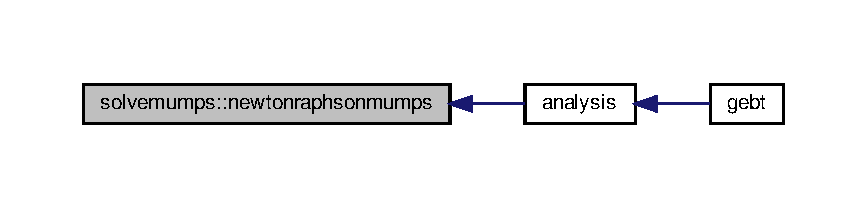
\includegraphics[width=350pt]{namespacesolvemumps_a243ff65847b437ecb22933d782df2db4_icgraph}
\end{center}
\end{figure}


\subsection{Variable Documentation}
\mbox{\Hypertarget{namespacesolvemumps_a5f812a31bb5931d66e5d6bb4c05f4a51}\label{namespacesolvemumps_a5f812a31bb5931d66e5d6bb4c05f4a51}} 
\index{solvemumps@{solvemumps}!ierr@{ierr}}
\index{ierr@{ierr}!solvemumps@{solvemumps}}
\subsubsection{\texorpdfstring{ierr}{ierr}}
{\footnotesize\ttfamily integer solvemumps\+::ierr}



error code of the M\+U\+M\+PS solver 



Definition at line 25 of file Solve\+Mumps.\+f90.

\mbox{\Hypertarget{namespacesolvemumps_ab76b5a7f705b0acb09ebc3ecf7e51f91}\label{namespacesolvemumps_ab76b5a7f705b0acb09ebc3ecf7e51f91}} 
\index{solvemumps@{solvemumps}!mumps\+\_\+par@{mumps\+\_\+par}}
\index{mumps\+\_\+par@{mumps\+\_\+par}!solvemumps@{solvemumps}}
\subsubsection{\texorpdfstring{mumps\+\_\+par}{mumps\_par}}
{\footnotesize\ttfamily type (dmumps\+\_\+struc) solvemumps\+::mumps\+\_\+par}



an array containing the configuration parameters of M\+U\+M\+PS solver 



Definition at line 24 of file Solve\+Mumps.\+f90.


\hypertarget{namespacesystem}{}\section{system Module Reference}
\label{namespacesystem}\index{system@{system}}


This module assemles the system including the coefficient matrix (jacobian matrix) and the right hand side (negative of the equation values) $\ast$.  


\subsection*{Functions/\+Subroutines}
\begin{DoxyCompactItemize}
\item 
subroutine, public \hyperlink{namespacesystem_aca86d62bded01533c138c9e2298cc804}{assemblejacobian} (ndof\+\_\+el, niter, memb\+\_\+info, v\+\_\+root\+\_\+a, omega\+\_\+a, member, error, ncond\+\_\+mb, mb\+\_\+condition, distr\+\_\+fun, dof\+\_\+con, x, aero\+\_\+flag, grav\+\_\+flag, init\+\_\+cond)
\begin{DoxyCompactList}\small\item\em Assemble the coefficient matrix of the beam system $\ast$. \end{DoxyCompactList}\item 
subroutine, public \hyperlink{namespacesystem_a442f9666f95d674029a7fbe213b47f8a}{assemblerhs} (ndof\+\_\+el, memb\+\_\+info, v\+\_\+root\+\_\+a, omega\+\_\+a, member, error, ncond\+\_\+mb, mb\+\_\+condition, distr\+\_\+fun, dof\+\_\+con, x, rhs, aero\+\_\+flag, grav\+\_\+flag, init\+\_\+cond)
\begin{DoxyCompactList}\small\item\em Assemble the right hand side. \end{DoxyCompactList}\item 
subroutine \hyperlink{namespacesystem_a048a8c1a606cebab7e33f3ae1877c31a}{pointfollowerj} (flag, nrow, ncol, e\+C\+Ttheta)
\begin{DoxyCompactList}\small\item\em Add the contribution to Jacobian matrix due to follower point force or moments. \end{DoxyCompactList}\end{DoxyCompactItemize}
\subsection*{Variables}
\begin{DoxyCompactItemize}
\item 
real(dbl), dimension(nstrn) \hyperlink{namespacesystem_a9db5b0f39df1dc763bd7885fa9f4389d}{x\+\_\+pt}
\begin{DoxyCompactList}\small\item\em the solution from the previous step for a key point. \end{DoxyCompactList}\item 
integer, dimension(nstrn) \hyperlink{namespacesystem_a1ec6fa7d33c56b907f960706f2c49a97}{kp\+\_\+dof}
\begin{DoxyCompactList}\small\item\em prescribed dof \end{DoxyCompactList}\item 
real(dbl), dimension(nstrn) \hyperlink{namespacesystem_a52739e5016f753e4d31c5f933aa2b79a}{kp\+\_\+cond}
\begin{DoxyCompactList}\small\item\em prescribed value \end{DoxyCompactList}\item 
integer, dimension(nstrn) \hyperlink{namespacesystem_af7b15e252e65635b4d03452e4c717697}{kp\+\_\+follower}
\begin{DoxyCompactList}\small\item\em follower condition \end{DoxyCompactList}\item 
integer, public \hyperlink{namespacesystem_a8c97c1868622a50b42869db23d0a2f11}{ne}
\begin{DoxyCompactList}\small\item\em Number of nonzero coefficients. \end{DoxyCompactList}\item 
integer, dimension(\+:), allocatable, public \hyperlink{namespacesystem_af8a50eade1073ff9c211526848dcec38}{irn}
\begin{DoxyCompactList}\small\item\em line index of nonzero coefficients \end{DoxyCompactList}\item 
integer, dimension(\+:), allocatable, public \hyperlink{namespacesystem_a32a5c04fae61a0d6a90727cd0bab43a7}{jcn}
\begin{DoxyCompactList}\small\item\em column index of nonzero coefficients \end{DoxyCompactList}\item 
real(dbl), dimension(\+:), allocatable, public \hyperlink{namespacesystem_ac5c6f08d5a21faff727c9a1240bae697}{coef}
\begin{DoxyCompactList}\small\item\em value of nonzero coefficients \end{DoxyCompactList}\end{DoxyCompactItemize}


\subsection{Detailed Description}
This module assemles the system including the coefficient matrix (jacobian matrix) and the right hand side (negative of the equation values) $\ast$. 

\subsection{Function/\+Subroutine Documentation}
\mbox{\Hypertarget{namespacesystem_aca86d62bded01533c138c9e2298cc804}\label{namespacesystem_aca86d62bded01533c138c9e2298cc804}} 
\index{system@{system}!assemblejacobian@{assemblejacobian}}
\index{assemblejacobian@{assemblejacobian}!system@{system}}
\subsubsection{\texorpdfstring{assemblejacobian()}{assemblejacobian()}}
{\footnotesize\ttfamily subroutine, public system\+::assemblejacobian (\begin{DoxyParamCaption}\item[{integer, intent(in)}]{ndof\+\_\+el,  }\item[{integer, intent(in)}]{niter,  }\item[{type (memberinf), dimension(\+:), intent(in)}]{memb\+\_\+info,  }\item[{real(dbl), dimension(\+:), intent(in)}]{v\+\_\+root\+\_\+a,  }\item[{real(dbl), dimension(\+:), intent(in)}]{omega\+\_\+a,  }\item[{integer, dimension(\+:,\+:), intent(in)}]{member,  }\item[{character($\ast$), intent(out)}]{error,  }\item[{integer, intent(in)}]{ncond\+\_\+mb,  }\item[{type(prescriinf), dimension(\+:), intent(in)}]{mb\+\_\+condition,  }\item[{real(dbl), dimension(\+:,\+:), intent(in)}]{distr\+\_\+fun,  }\item[{integer, dimension(\+:)}]{dof\+\_\+con,  }\item[{real(dbl), dimension(\+:), intent(in)}]{x,  }\item[{integer, intent(in)}]{aero\+\_\+flag,  }\item[{integer, intent(in)}]{grav\+\_\+flag,  }\item[{real(dbl), dimension(\+:,\+:), intent(in), optional}]{init\+\_\+cond }\end{DoxyParamCaption})}



Assemble the coefficient matrix of the beam system $\ast$. 


\begin{DoxyParams}[1]{Parameters}
\mbox{\tt in}  & {\em ndof\+\_\+el} & \hyperlink{namespaceioaero_a2b095b5cb5aab1f100d202c8004c9cb5}{ioaero\+::ndof\+\_\+el}\\
\hline
\mbox{\tt in}  & {\em niter} & \hyperlink{namespaceioaero_ac008486fd12e0029a1ef77b3ca5e12c3}{ioaero\+::niter}\\
\hline
\mbox{\tt in}  & {\em aero\+\_\+flag} & \hyperlink{namespaceioaero_afb280b6ca8de323c9a07076df81a71e1}{ioaero\+::aero\+\_\+flag}\\
\hline
\mbox{\tt in}  & {\em grav\+\_\+flag} & \hyperlink{namespaceioaero_a831fe87d45ef05e3e29a8c4c2fc88c8f}{ioaero\+::grav\+\_\+flag}\\
\hline
\mbox{\tt in}  & {\em v\+\_\+root\+\_\+a} & linear velocity of frame a\\
\hline
\mbox{\tt in}  & {\em omega\+\_\+a} & angular velocity of frame a\\
\hline
\mbox{\tt in}  & {\em memb\+\_\+info} & contains the member parameters of the whole structure\\
\hline
\mbox{\tt in}  & {\em distr\+\_\+fun} & \hyperlink{namespaceioaero_a1d7c3689e30c2925cd403a84e9176242}{ioaero\+::distr\+\_\+fun}\\
\hline
\mbox{\tt in}  & {\em member} & \hyperlink{namespaceioaero_ae040b39fe109c45b001985415e230ec3}{ioaero\+::member}\\
\hline
\mbox{\tt in}  & {\em ncond\+\_\+mb} & \hyperlink{namespaceioaero_ab9193f4ff70a22ae5858118fc653f22b}{ioaero\+::ncond\+\_\+mb}\\
\hline
 & {\em dof\+\_\+con} & note dof\+\_\+con is passed by value, hence what is changed in this subroutine will not affect the original value.\\
\hline
\mbox{\tt in}  & {\em x} & solution vector\\
\hline
\mbox{\tt in}  & {\em mb\+\_\+condition} & \hyperlink{namespaceioaero_a2463929ef049b49fe7b49011c66cc806}{ioaero\+::mb\+\_\+condition}\\
\hline
\mbox{\tt out}  & {\em error} & \hyperlink{namespaceioaero_aebd85ae2a176f49a7213d8ed7b68f887}{ioaero\+::error}\\
\hline
\mbox{\tt in}  & {\em init\+\_\+cond} & \hyperlink{namespaceioaero_ad88d83709eb2f4596a89098db11ba770}{ioaero\+::init\+\_\+cond} \\
\hline
\end{DoxyParams}


Definition at line 48 of file System.\+f90.

Here is the caller graph for this function\+:\nopagebreak
\begin{figure}[H]
\begin{center}
\leavevmode
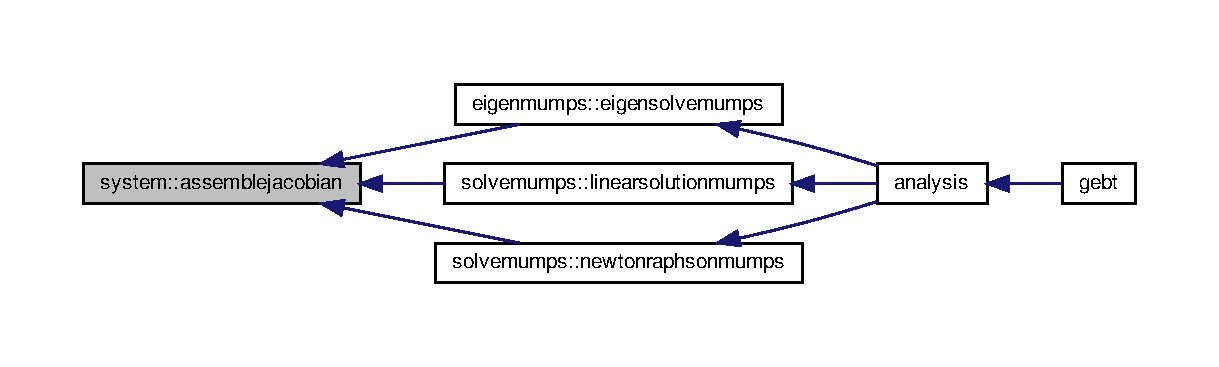
\includegraphics[width=350pt]{namespacesystem_aca86d62bded01533c138c9e2298cc804_icgraph}
\end{center}
\end{figure}
\mbox{\Hypertarget{namespacesystem_a442f9666f95d674029a7fbe213b47f8a}\label{namespacesystem_a442f9666f95d674029a7fbe213b47f8a}} 
\index{system@{system}!assemblerhs@{assemblerhs}}
\index{assemblerhs@{assemblerhs}!system@{system}}
\subsubsection{\texorpdfstring{assemblerhs()}{assemblerhs()}}
{\footnotesize\ttfamily subroutine, public system\+::assemblerhs (\begin{DoxyParamCaption}\item[{integer, intent(in)}]{ndof\+\_\+el,  }\item[{type (memberinf), dimension(\+:), intent(in)}]{memb\+\_\+info,  }\item[{real(dbl), dimension(\+:), intent(in)}]{v\+\_\+root\+\_\+a,  }\item[{real(dbl), dimension(\+:), intent(in)}]{omega\+\_\+a,  }\item[{integer, dimension(\+:,\+:), intent(in)}]{member,  }\item[{character($\ast$), intent(out)}]{error,  }\item[{integer, intent(in)}]{ncond\+\_\+mb,  }\item[{type(prescriinf), dimension(\+:), intent(in)}]{mb\+\_\+condition,  }\item[{real(dbl), dimension(\+:,\+:), intent(in)}]{distr\+\_\+fun,  }\item[{integer, dimension(\+:)}]{dof\+\_\+con,  }\item[{real(dbl), dimension(\+:), intent(in)}]{x,  }\item[{real(dbl), dimension(\+:), intent(out)}]{rhs,  }\item[{integer, intent(in)}]{aero\+\_\+flag,  }\item[{integer, intent(in)}]{grav\+\_\+flag,  }\item[{real(dbl), dimension(\+:,\+:), intent(in), optional}]{init\+\_\+cond }\end{DoxyParamCaption})}



Assemble the right hand side. 


\begin{DoxyParams}[1]{Parameters}
\mbox{\tt in}  & {\em ndof\+\_\+el} & \hyperlink{namespaceioaero_a2b095b5cb5aab1f100d202c8004c9cb5}{ioaero\+::ndof\+\_\+el}\\
\hline
\mbox{\tt in}  & {\em aero\+\_\+flag} & \hyperlink{namespaceioaero_afb280b6ca8de323c9a07076df81a71e1}{ioaero\+::aero\+\_\+flag}\\
\hline
\mbox{\tt in}  & {\em grav\+\_\+flag} & \hyperlink{namespaceioaero_a831fe87d45ef05e3e29a8c4c2fc88c8f}{ioaero\+::grav\+\_\+flag}\\
\hline
\mbox{\tt in}  & {\em memb\+\_\+info} & contains the member parameters of the whole structure\\
\hline
\mbox{\tt in}  & {\em v\+\_\+root\+\_\+a} & linear velocity of frame a\\
\hline
\mbox{\tt in}  & {\em omega\+\_\+a} & angular velocity of frame a\\
\hline
\mbox{\tt in}  & {\em distr\+\_\+fun} & \hyperlink{namespaceioaero_a1d7c3689e30c2925cd403a84e9176242}{ioaero\+::distr\+\_\+fun}\\
\hline
\mbox{\tt in}  & {\em member} & \hyperlink{namespaceioaero_ae040b39fe109c45b001985415e230ec3}{ioaero\+::member}\\
\hline
\mbox{\tt in}  & {\em ncond\+\_\+mb} & \hyperlink{namespaceioaero_ab9193f4ff70a22ae5858118fc653f22b}{ioaero\+::ncond\+\_\+mb}\\
\hline
\mbox{\tt in}  & {\em x} & solution vector\\
\hline
\mbox{\tt in}  & {\em mb\+\_\+condition} & \hyperlink{namespaceioaero_a2463929ef049b49fe7b49011c66cc806}{ioaero\+::mb\+\_\+condition}\\
\hline
\mbox{\tt in}  & {\em init\+\_\+cond} & \hyperlink{namespaceioaero_ad88d83709eb2f4596a89098db11ba770}{ioaero\+::init\+\_\+cond} \\
\hline
\end{DoxyParams}


Definition at line 321 of file System.\+f90.

Here is the caller graph for this function\+:\nopagebreak
\begin{figure}[H]
\begin{center}
\leavevmode
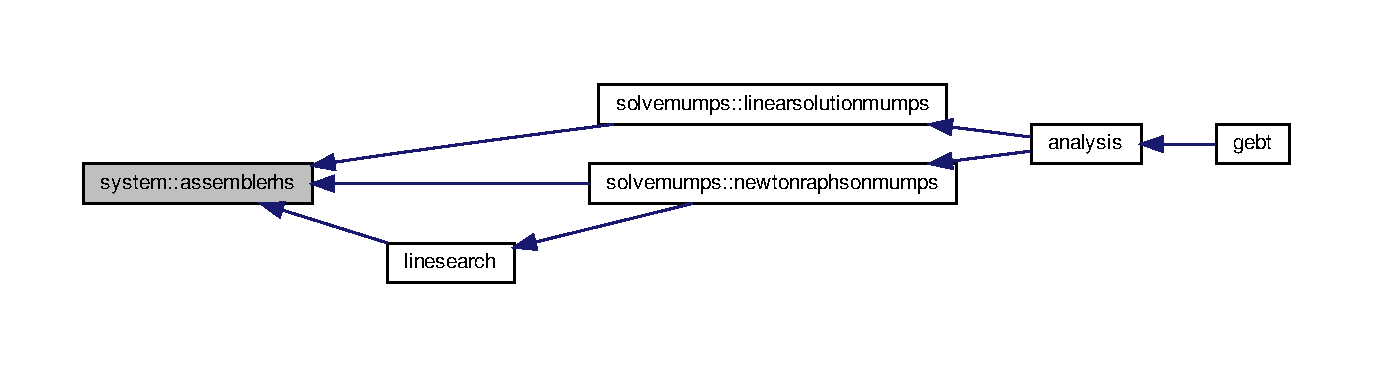
\includegraphics[width=350pt]{namespacesystem_a442f9666f95d674029a7fbe213b47f8a_icgraph}
\end{center}
\end{figure}
\mbox{\Hypertarget{namespacesystem_a048a8c1a606cebab7e33f3ae1877c31a}\label{namespacesystem_a048a8c1a606cebab7e33f3ae1877c31a}} 
\index{system@{system}!pointfollowerj@{pointfollowerj}}
\index{pointfollowerj@{pointfollowerj}!system@{system}}
\subsubsection{\texorpdfstring{pointfollowerj()}{pointfollowerj()}}
{\footnotesize\ttfamily subroutine system\+::pointfollowerj (\begin{DoxyParamCaption}\item[{integer, intent(in)}]{flag,  }\item[{integer, intent(in)}]{nrow,  }\item[{integer, intent(in)}]{ncol,  }\item[{real(dbl), dimension(\+:,\+:,\+:), intent(in)}]{e\+C\+Ttheta }\end{DoxyParamCaption})\hspace{0.3cm}{\ttfamily [private]}}



Add the contribution to Jacobian matrix due to follower point force or moments. 



Definition at line 502 of file System.\+f90.

Here is the caller graph for this function\+:\nopagebreak
\begin{figure}[H]
\begin{center}
\leavevmode
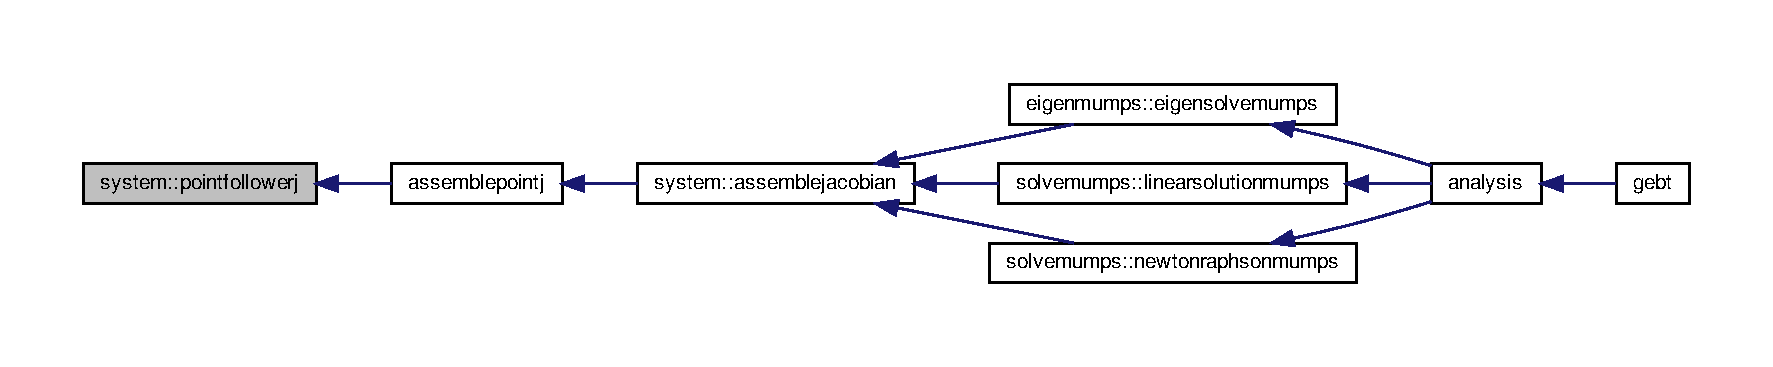
\includegraphics[width=350pt]{namespacesystem_a048a8c1a606cebab7e33f3ae1877c31a_icgraph}
\end{center}
\end{figure}


\subsection{Variable Documentation}
\mbox{\Hypertarget{namespacesystem_ac5c6f08d5a21faff727c9a1240bae697}\label{namespacesystem_ac5c6f08d5a21faff727c9a1240bae697}} 
\index{system@{system}!coef@{coef}}
\index{coef@{coef}!system@{system}}
\subsubsection{\texorpdfstring{coef}{coef}}
{\footnotesize\ttfamily real(dbl), dimension(\+:), allocatable, public system\+::coef}



value of nonzero coefficients 



Definition at line 35 of file System.\+f90.

\mbox{\Hypertarget{namespacesystem_af8a50eade1073ff9c211526848dcec38}\label{namespacesystem_af8a50eade1073ff9c211526848dcec38}} 
\index{system@{system}!irn@{irn}}
\index{irn@{irn}!system@{system}}
\subsubsection{\texorpdfstring{irn}{irn}}
{\footnotesize\ttfamily integer, dimension(\+:), allocatable, public system\+::irn}



line index of nonzero coefficients 



Definition at line 33 of file System.\+f90.

\mbox{\Hypertarget{namespacesystem_a32a5c04fae61a0d6a90727cd0bab43a7}\label{namespacesystem_a32a5c04fae61a0d6a90727cd0bab43a7}} 
\index{system@{system}!jcn@{jcn}}
\index{jcn@{jcn}!system@{system}}
\subsubsection{\texorpdfstring{jcn}{jcn}}
{\footnotesize\ttfamily integer, dimension(\+:), allocatable, public system\+::jcn}



column index of nonzero coefficients 



Definition at line 34 of file System.\+f90.

\mbox{\Hypertarget{namespacesystem_a52739e5016f753e4d31c5f933aa2b79a}\label{namespacesystem_a52739e5016f753e4d31c5f933aa2b79a}} 
\index{system@{system}!kp\+\_\+cond@{kp\+\_\+cond}}
\index{kp\+\_\+cond@{kp\+\_\+cond}!system@{system}}
\subsubsection{\texorpdfstring{kp\+\_\+cond}{kp\_cond}}
{\footnotesize\ttfamily real(dbl), dimension(nstrn) system\+::kp\+\_\+cond\hspace{0.3cm}{\ttfamily [private]}}



prescribed value 



Definition at line 29 of file System.\+f90.

\mbox{\Hypertarget{namespacesystem_a1ec6fa7d33c56b907f960706f2c49a97}\label{namespacesystem_a1ec6fa7d33c56b907f960706f2c49a97}} 
\index{system@{system}!kp\+\_\+dof@{kp\+\_\+dof}}
\index{kp\+\_\+dof@{kp\+\_\+dof}!system@{system}}
\subsubsection{\texorpdfstring{kp\+\_\+dof}{kp\_dof}}
{\footnotesize\ttfamily integer, dimension(nstrn) system\+::kp\+\_\+dof\hspace{0.3cm}{\ttfamily [private]}}



prescribed dof 



Definition at line 28 of file System.\+f90.

\mbox{\Hypertarget{namespacesystem_af7b15e252e65635b4d03452e4c717697}\label{namespacesystem_af7b15e252e65635b4d03452e4c717697}} 
\index{system@{system}!kp\+\_\+follower@{kp\+\_\+follower}}
\index{kp\+\_\+follower@{kp\+\_\+follower}!system@{system}}
\subsubsection{\texorpdfstring{kp\+\_\+follower}{kp\_follower}}
{\footnotesize\ttfamily integer, dimension(nstrn) system\+::kp\+\_\+follower\hspace{0.3cm}{\ttfamily [private]}}



follower condition 



Definition at line 30 of file System.\+f90.

\mbox{\Hypertarget{namespacesystem_a8c97c1868622a50b42869db23d0a2f11}\label{namespacesystem_a8c97c1868622a50b42869db23d0a2f11}} 
\index{system@{system}!ne@{ne}}
\index{ne@{ne}!system@{system}}
\subsubsection{\texorpdfstring{ne}{ne}}
{\footnotesize\ttfamily integer, public system\+::ne}



Number of nonzero coefficients. 



Definition at line 32 of file System.\+f90.

\mbox{\Hypertarget{namespacesystem_a9db5b0f39df1dc763bd7885fa9f4389d}\label{namespacesystem_a9db5b0f39df1dc763bd7885fa9f4389d}} 
\index{system@{system}!x\+\_\+pt@{x\+\_\+pt}}
\index{x\+\_\+pt@{x\+\_\+pt}!system@{system}}
\subsubsection{\texorpdfstring{x\+\_\+pt}{x\_pt}}
{\footnotesize\ttfamily real(dbl), dimension(nstrn) system\+::x\+\_\+pt\hspace{0.3cm}{\ttfamily [private]}}



the solution from the previous step for a key point. 



Definition at line 27 of file System.\+f90.


\hypertarget{namespacetimefunctionmodule}{}\section{timefunctionmodule Module Reference}
\label{namespacetimefunctionmodule}\index{timefunctionmodule@{timefunctionmodule}}


A module for defining time functions needed for both prescribed concentrated and distributed conditions.  


\subsection*{Data Types}
\begin{DoxyCompactItemize}
\item 
type \hyperlink{structtimefunctionmodule_1_1timefunction}{timefunction}
\end{DoxyCompactItemize}
\subsection*{Functions/\+Subroutines}
\begin{DoxyCompactItemize}
\item 
real(dbl) function, public \hyperlink{namespacetimefunctionmodule_a177d2096c59b79cbbfd85b4e05b57f29}{gettimefunction} (tf, t)
\begin{DoxyCompactList}\small\item\em get the time function value for any arbitrary time from a piecewise linear function or harmonic function decide where t is located, then interpret the value \end{DoxyCompactList}\item 
elemental type(\hyperlink{structtimefunctionmodule_1_1timefunction}{timefunction}) function, public \hyperlink{namespacetimefunctionmodule_a4a9a0cfa8fd5fc6dcfd21c0eeed2a027}{inittf} ()
\begin{DoxyCompactList}\small\item\em Initialize the time function. \end{DoxyCompactList}\item 
type(\hyperlink{structtimefunctionmodule_1_1timefunction}{timefunction}) function, public \hyperlink{namespacetimefunctionmodule_a9dc9317deeac617a45cf48f6101f11d2}{inputechotimefunctions} (IN, E\+IN, error)
\begin{DoxyCompactList}\small\item\em Input and echo Time Functions. \end{DoxyCompactList}\item 
real(dbl) function, dimension(size(vec)), public \hyperlink{namespacetimefunctionmodule_a907e0921288aa4f538e605c521686e4a}{currentvalues} (vec, vec\+\_\+tf, time\+\_\+fun, time\+\_\+current)
\begin{DoxyCompactList}\small\item\em Evaluate current function based on magnitude and time. \end{DoxyCompactList}\end{DoxyCompactItemize}


\subsection{Detailed Description}
A module for defining time functions needed for both prescribed concentrated and distributed conditions. 

\subsection{Function/\+Subroutine Documentation}
\mbox{\Hypertarget{namespacetimefunctionmodule_a907e0921288aa4f538e605c521686e4a}\label{namespacetimefunctionmodule_a907e0921288aa4f538e605c521686e4a}} 
\index{timefunctionmodule@{timefunctionmodule}!currentvalues@{currentvalues}}
\index{currentvalues@{currentvalues}!timefunctionmodule@{timefunctionmodule}}
\subsubsection{\texorpdfstring{currentvalues()}{currentvalues()}}
{\footnotesize\ttfamily real(dbl) function, dimension(size(vec)), public timefunctionmodule\+::currentvalues (\begin{DoxyParamCaption}\item[{real(dbl), dimension(\+:), intent(in)}]{vec,  }\item[{integer, dimension(\+:), intent(in)}]{vec\+\_\+tf,  }\item[{type (\hyperlink{structtimefunctionmodule_1_1timefunction}{timefunction}), dimension(\+:), intent(in)}]{time\+\_\+fun,  }\item[{real(dbl), intent(in)}]{time\+\_\+current }\end{DoxyParamCaption})}



Evaluate current function based on magnitude and time. 



Definition at line 202 of file Time\+Function.\+f90.

Here is the caller graph for this function\+:\nopagebreak
\begin{figure}[H]
\begin{center}
\leavevmode
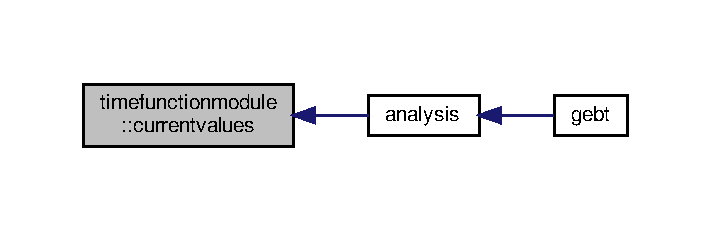
\includegraphics[width=341pt]{namespacetimefunctionmodule_a907e0921288aa4f538e605c521686e4a_icgraph}
\end{center}
\end{figure}
\mbox{\Hypertarget{namespacetimefunctionmodule_a177d2096c59b79cbbfd85b4e05b57f29}\label{namespacetimefunctionmodule_a177d2096c59b79cbbfd85b4e05b57f29}} 
\index{timefunctionmodule@{timefunctionmodule}!gettimefunction@{gettimefunction}}
\index{gettimefunction@{gettimefunction}!timefunctionmodule@{timefunctionmodule}}
\subsubsection{\texorpdfstring{gettimefunction()}{gettimefunction()}}
{\footnotesize\ttfamily real(dbl) function, public timefunctionmodule\+::gettimefunction (\begin{DoxyParamCaption}\item[{type (\hyperlink{structtimefunctionmodule_1_1timefunction}{timefunction}), intent(in)}]{tf,  }\item[{real(dbl), intent(in)}]{t }\end{DoxyParamCaption})}



get the time function value for any arbitrary time from a piecewise linear function or harmonic function decide where t is located, then interpret the value 



Definition at line 44 of file Time\+Function.\+f90.

Here is the caller graph for this function\+:\nopagebreak
\begin{figure}[H]
\begin{center}
\leavevmode
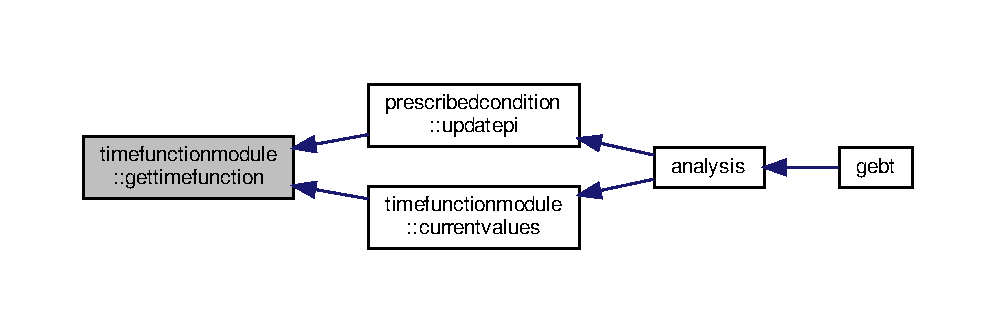
\includegraphics[width=350pt]{namespacetimefunctionmodule_a177d2096c59b79cbbfd85b4e05b57f29_icgraph}
\end{center}
\end{figure}
\mbox{\Hypertarget{namespacetimefunctionmodule_a4a9a0cfa8fd5fc6dcfd21c0eeed2a027}\label{namespacetimefunctionmodule_a4a9a0cfa8fd5fc6dcfd21c0eeed2a027}} 
\index{timefunctionmodule@{timefunctionmodule}!inittf@{inittf}}
\index{inittf@{inittf}!timefunctionmodule@{timefunctionmodule}}
\subsubsection{\texorpdfstring{inittf()}{inittf()}}
{\footnotesize\ttfamily elemental type (\hyperlink{structtimefunctionmodule_1_1timefunction}{timefunction}) function, public timefunctionmodule\+::inittf (\begin{DoxyParamCaption}{ }\end{DoxyParamCaption})}



Initialize the time function. 



Definition at line 104 of file Time\+Function.\+f90.

Here is the caller graph for this function\+:\nopagebreak
\begin{figure}[H]
\begin{center}
\leavevmode
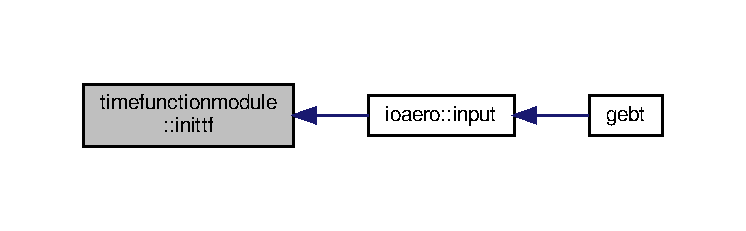
\includegraphics[width=350pt]{namespacetimefunctionmodule_a4a9a0cfa8fd5fc6dcfd21c0eeed2a027_icgraph}
\end{center}
\end{figure}
\mbox{\Hypertarget{namespacetimefunctionmodule_a9dc9317deeac617a45cf48f6101f11d2}\label{namespacetimefunctionmodule_a9dc9317deeac617a45cf48f6101f11d2}} 
\index{timefunctionmodule@{timefunctionmodule}!inputechotimefunctions@{inputechotimefunctions}}
\index{inputechotimefunctions@{inputechotimefunctions}!timefunctionmodule@{timefunctionmodule}}
\subsubsection{\texorpdfstring{inputechotimefunctions()}{inputechotimefunctions()}}
{\footnotesize\ttfamily type (\hyperlink{structtimefunctionmodule_1_1timefunction}{timefunction}) function, public timefunctionmodule\+::inputechotimefunctions (\begin{DoxyParamCaption}\item[{integer, intent(in)}]{IN,  }\item[{integer, intent(in)}]{E\+IN,  }\item[{character($\ast$), intent(out)}]{error }\end{DoxyParamCaption})}



Input and echo Time Functions. 


\begin{DoxyParams}[1]{Parameters}
\mbox{\tt in}  & {\em ein} & file units for input anf echo files, respectively \\
\hline
\end{DoxyParams}


Definition at line 124 of file Time\+Function.\+f90.

Here is the caller graph for this function\+:\nopagebreak
\begin{figure}[H]
\begin{center}
\leavevmode
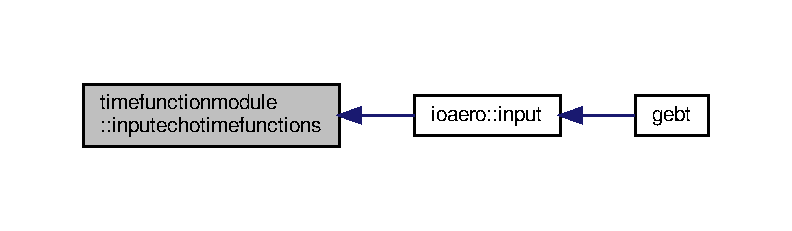
\includegraphics[width=350pt]{namespacetimefunctionmodule_a9dc9317deeac617a45cf48f6101f11d2_icgraph}
\end{center}
\end{figure}

\hypertarget{namespaceutils}{}\section{utils Namespace Reference}
\label{namespaceutils}\index{utils@{utils}}


The package contains a set of functions used by several classes.  




\subsection{Detailed Description}
The package contains a set of functions used by several classes. 


\chapter{Data Type Documentation}
\hypertarget{classgebtaero_1_1_composite_box_1_1_composite_box}{}\section{gebtaero.\+Composite\+Box.\+Composite\+Box Class Reference}
\label{classgebtaero_1_1_composite_box_1_1_composite_box}\index{gebtaero.\+Composite\+Box.\+Composite\+Box@{gebtaero.\+Composite\+Box.\+Composite\+Box}}


Class interfacing the solver with 3D F\+EM calculix computation to obtain the cross section parameter from a composite box.  


\subsection*{Public Member Functions}
\begin{DoxyCompactItemize}
\item 
def \hyperlink{classgebtaero_1_1_composite_box_1_1_composite_box_a64c4292dbd036313813fc00a78fb13cb}{\+\_\+\+\_\+init\+\_\+\+\_\+} (self, \hyperlink{classgebtaero_1_1_composite_box_1_1_composite_box_a7bfe2dab84e5ae8d8cdba1337b89c309}{Left}, \hyperlink{classgebtaero_1_1_composite_box_1_1_composite_box_a61cdca93cc1f5ef451192395fc50b67b}{Right}, \hyperlink{classgebtaero_1_1_composite_box_1_1_composite_box_a4c043150a29d71b986a91f21be6a4e47}{Up}, \hyperlink{classgebtaero_1_1_composite_box_1_1_composite_box_ad1559917cabe3fcb6c05bf603d8b0b0c}{Down}, \hyperlink{classgebtaero_1_1_composite_box_1_1_composite_box_a44593d7302ceb1c46ac637437b5e1061}{Width}, \hyperlink{classgebtaero_1_1_composite_box_1_1_composite_box_affc2b38183c3b0ec7534629cf63e4cc5}{Height}, \hyperlink{classgebtaero_1_1_composite_box_1_1_composite_box_a26fcf7763030afb28f45f2354125c352}{OffsetY}=0., \hyperlink{classgebtaero_1_1_composite_box_1_1_composite_box_a50e38078e66133a95f34f2d9176329d9}{OffsetZ}=0.)
\begin{DoxyCompactList}\small\item\em Composite box constructor; It contains 4 \hyperlink{namespacegebtaero_1_1_composite_plate}{Composite\+Plate}; modify the chord of left and right wall. \end{DoxyCompactList}\item 
def \hyperlink{classgebtaero_1_1_composite_box_1_1_composite_box_a80477ea79acc12d0d45970d6c0b208d6}{Get\+Offsets} (self)
\item 
def \hyperlink{classgebtaero_1_1_composite_box_1_1_composite_box_a227089b18b5436fdba7853cbe1071a99}{Get\+Width} (self)
\item 
def \hyperlink{classgebtaero_1_1_composite_box_1_1_composite_box_a8ca332752a2b78ca0ba4c65f99ab1b62}{Get\+Height} (self)
\item 
def \hyperlink{classgebtaero_1_1_composite_box_1_1_composite_box_af2465d364bb51056af14fde13bd05d4a}{Create\+Fbd\+File} (self, Type\+Elem, Nb\+ElemX, Nb\+Elem\+YZ, Nb\+Elem\+Ply)
\begin{DoxyCompactList}\small\item\em Create the input file for cgx preprocessor. \end{DoxyCompactList}\item 
def \hyperlink{classgebtaero_1_1_composite_box_1_1_composite_box_a005e7c9de0e4307ad9ff7ed4e8f7c8a4}{Create\+Inp\+File} (self, Stress=False, Plane\+Section=False, Disp=0)
\begin{DoxyCompactList}\small\item\em Create the input file for ccx solver. \end{DoxyCompactList}\item 
def \hyperlink{classgebtaero_1_1_composite_box_1_1_composite_box_a6b944eeef7002377d7b83c5dd6ae6550}{Compute\+Mass\+Matrix} (self, \hyperlink{classgebtaero_1_1_composite_box_1_1_composite_box_a26fcf7763030afb28f45f2354125c352}{OffsetY}=0., \hyperlink{classgebtaero_1_1_composite_box_1_1_composite_box_a50e38078e66133a95f34f2d9176329d9}{OffsetZ}=0.)
\begin{DoxyCompactList}\small\item\em Compute the \hyperlink{classgebtaero_1_1_cross_section_1_1_cross_section_ae9be8649853163b2b4dfdaa3584d9f78}{Cross\+Section\+::\+Mass\+Matrix} using the mass matrix of the 4 walls of the box. \end{DoxyCompactList}\item 
def \hyperlink{classgebtaero_1_1_composite_box_1_1_composite_box_a9328777b54ead0767f0075fe599b09d9}{Create\+Periodic\+Eq} (self)
\begin{DoxyCompactList}\small\item\em Interface to the utils subroutine \hyperlink{namespacegebtaero_1_1utils_a4f786ecbe66af9f64c802adf4e0a990f}{utils\+::\+Create\+Periodic\+Eq}. \end{DoxyCompactList}\item 
def \hyperlink{classgebtaero_1_1_composite_box_1_1_composite_box_a024d2118868a02e7e6218300435148e0}{Display\+Section\+Deformation} (self, Type\+Elem, Nb\+ElemX, Nb\+Elem\+YZ, Nb\+Elem\+Ply, Def\+Type, Plane\+Section=False)
\begin{DoxyCompactList}\small\item\em Launch the cgx postprocessor with a particular elementary load case. \end{DoxyCompactList}\end{DoxyCompactItemize}
\subsection*{Public Attributes}
\begin{DoxyCompactItemize}
\item 
\hyperlink{classgebtaero_1_1_composite_box_1_1_composite_box_a7bfe2dab84e5ae8d8cdba1337b89c309}{Left}
\begin{DoxyCompactList}\small\item\em Left wall of the box (\hyperlink{namespacegebtaero_1_1_composite_plate}{Composite\+Plate}) \end{DoxyCompactList}\item 
\hyperlink{classgebtaero_1_1_composite_box_1_1_composite_box_a61cdca93cc1f5ef451192395fc50b67b}{Right}
\begin{DoxyCompactList}\small\item\em Right wall of the box (\hyperlink{namespacegebtaero_1_1_composite_plate}{Composite\+Plate}) \end{DoxyCompactList}\item 
\hyperlink{classgebtaero_1_1_composite_box_1_1_composite_box_a4c043150a29d71b986a91f21be6a4e47}{Up}
\begin{DoxyCompactList}\small\item\em Up wall of the box (\hyperlink{namespacegebtaero_1_1_composite_plate}{Composite\+Plate}) \end{DoxyCompactList}\item 
\hyperlink{classgebtaero_1_1_composite_box_1_1_composite_box_ad1559917cabe3fcb6c05bf603d8b0b0c}{Down}
\begin{DoxyCompactList}\small\item\em Down wall of the box (\hyperlink{namespacegebtaero_1_1_composite_plate}{Composite\+Plate}) \end{DoxyCompactList}\item 
\hyperlink{classgebtaero_1_1_composite_box_1_1_composite_box_a44593d7302ceb1c46ac637437b5e1061}{Width}
\begin{DoxyCompactList}\small\item\em Width of the box (m) \end{DoxyCompactList}\item 
\hyperlink{classgebtaero_1_1_composite_box_1_1_composite_box_affc2b38183c3b0ec7534629cf63e4cc5}{Height}
\begin{DoxyCompactList}\small\item\em Height height of the box (m) \end{DoxyCompactList}\item 
\hyperlink{classgebtaero_1_1_composite_box_1_1_composite_box_a26fcf7763030afb28f45f2354125c352}{OffsetY}
\begin{DoxyCompactList}\small\item\em Y coordinate of the box center in the \hyperlink{namespacegebtaero_1_1_frame}{Frame} B. \end{DoxyCompactList}\item 
\hyperlink{classgebtaero_1_1_composite_box_1_1_composite_box_a50e38078e66133a95f34f2d9176329d9}{OffsetZ}
\begin{DoxyCompactList}\small\item\em Z coordinate of the box center in the \hyperlink{namespacegebtaero_1_1_frame}{Frame} B. \end{DoxyCompactList}\end{DoxyCompactItemize}


\subsection{Detailed Description}
Class interfacing the solver with 3D F\+EM calculix computation to obtain the cross section parameter from a composite box. 

Definition at line 9 of file Composite\+Box.\+py.



\subsection{Constructor \& Destructor Documentation}
\mbox{\Hypertarget{classgebtaero_1_1_composite_box_1_1_composite_box_a64c4292dbd036313813fc00a78fb13cb}\label{classgebtaero_1_1_composite_box_1_1_composite_box_a64c4292dbd036313813fc00a78fb13cb}} 
\index{gebtaero\+::\+Composite\+Box\+::\+Composite\+Box@{gebtaero\+::\+Composite\+Box\+::\+Composite\+Box}!\+\_\+\+\_\+init\+\_\+\+\_\+@{\+\_\+\+\_\+init\+\_\+\+\_\+}}
\index{\+\_\+\+\_\+init\+\_\+\+\_\+@{\+\_\+\+\_\+init\+\_\+\+\_\+}!gebtaero\+::\+Composite\+Box\+::\+Composite\+Box@{gebtaero\+::\+Composite\+Box\+::\+Composite\+Box}}
\subsubsection{\texorpdfstring{\+\_\+\+\_\+init\+\_\+\+\_\+()}{\_\_init\_\_()}}
{\footnotesize\ttfamily def gebtaero.\+Composite\+Box.\+Composite\+Box.\+\_\+\+\_\+init\+\_\+\+\_\+ (\begin{DoxyParamCaption}\item[{}]{self,  }\item[{}]{Left,  }\item[{}]{Right,  }\item[{}]{Up,  }\item[{}]{Down,  }\item[{}]{Width,  }\item[{}]{Height,  }\item[{}]{OffsetY = {\ttfamily 0.},  }\item[{}]{OffsetZ = {\ttfamily 0.} }\end{DoxyParamCaption})}



Composite box constructor; It contains 4 \hyperlink{namespacegebtaero_1_1_composite_plate}{Composite\+Plate}; modify the chord of left and right wall. 



Definition at line 11 of file Composite\+Box.\+py.



\subsection{Member Function Documentation}
\mbox{\Hypertarget{classgebtaero_1_1_composite_box_1_1_composite_box_a6b944eeef7002377d7b83c5dd6ae6550}\label{classgebtaero_1_1_composite_box_1_1_composite_box_a6b944eeef7002377d7b83c5dd6ae6550}} 
\index{gebtaero\+::\+Composite\+Box\+::\+Composite\+Box@{gebtaero\+::\+Composite\+Box\+::\+Composite\+Box}!Compute\+Mass\+Matrix@{Compute\+Mass\+Matrix}}
\index{Compute\+Mass\+Matrix@{Compute\+Mass\+Matrix}!gebtaero\+::\+Composite\+Box\+::\+Composite\+Box@{gebtaero\+::\+Composite\+Box\+::\+Composite\+Box}}
\subsubsection{\texorpdfstring{Compute\+Mass\+Matrix()}{ComputeMassMatrix()}}
{\footnotesize\ttfamily def gebtaero.\+Composite\+Box.\+Composite\+Box.\+Compute\+Mass\+Matrix (\begin{DoxyParamCaption}\item[{}]{self,  }\item[{}]{OffsetY = {\ttfamily 0.},  }\item[{}]{OffsetZ = {\ttfamily 0.} }\end{DoxyParamCaption})}



Compute the \hyperlink{classgebtaero_1_1_cross_section_1_1_cross_section_ae9be8649853163b2b4dfdaa3584d9f78}{Cross\+Section\+::\+Mass\+Matrix} using the mass matrix of the 4 walls of the box. 

\begin{DoxyReturn}{Returns}
Mu Mass per unit length (kg/m) 

I22 mass moment of inertia around yB (bending span-\/wise, kg.\+m) 

I33 mass moment of inertia around zB (bending chord-\/wise, kg.\+m) 

I23 product of inertia in plane (yB,zB) 

Ycg Y coordinate of the Center of Gravity in frame B 

Zcg Z coordinate of the Center of Gravity in frame B 
\end{DoxyReturn}


Definition at line 311 of file Composite\+Box.\+py.

\mbox{\Hypertarget{classgebtaero_1_1_composite_box_1_1_composite_box_af2465d364bb51056af14fde13bd05d4a}\label{classgebtaero_1_1_composite_box_1_1_composite_box_af2465d364bb51056af14fde13bd05d4a}} 
\index{gebtaero\+::\+Composite\+Box\+::\+Composite\+Box@{gebtaero\+::\+Composite\+Box\+::\+Composite\+Box}!Create\+Fbd\+File@{Create\+Fbd\+File}}
\index{Create\+Fbd\+File@{Create\+Fbd\+File}!gebtaero\+::\+Composite\+Box\+::\+Composite\+Box@{gebtaero\+::\+Composite\+Box\+::\+Composite\+Box}}
\subsubsection{\texorpdfstring{Create\+Fbd\+File()}{CreateFbdFile()}}
{\footnotesize\ttfamily def gebtaero.\+Composite\+Box.\+Composite\+Box.\+Create\+Fbd\+File (\begin{DoxyParamCaption}\item[{}]{self,  }\item[{}]{Type\+Elem,  }\item[{}]{Nb\+ElemX,  }\item[{}]{Nb\+Elem\+YZ,  }\item[{}]{Nb\+Elem\+Ply }\end{DoxyParamCaption})}



Create the input file for cgx preprocessor. 


\begin{DoxyParams}{Parameters}
{\em Type\+Elem} & the type of finite element used for the computation. Supported \+: he20r, he20, he8i, he8, pe15 (see ccx doc) \\
\hline
{\em Nb\+ElemX} & the number of finite element in the beam direction (for a constant cross section, 1 element is enough) \\
\hline
{\em N\+B\+Elem\+YZ} & the number of finite element along the wall directions \\
\hline
{\em N\+B\+Elem\+Ply} & the number of finite element in a composite ply \\
\hline
\end{DoxyParams}


Definition at line 47 of file Composite\+Box.\+py.

\mbox{\Hypertarget{classgebtaero_1_1_composite_box_1_1_composite_box_a005e7c9de0e4307ad9ff7ed4e8f7c8a4}\label{classgebtaero_1_1_composite_box_1_1_composite_box_a005e7c9de0e4307ad9ff7ed4e8f7c8a4}} 
\index{gebtaero\+::\+Composite\+Box\+::\+Composite\+Box@{gebtaero\+::\+Composite\+Box\+::\+Composite\+Box}!Create\+Inp\+File@{Create\+Inp\+File}}
\index{Create\+Inp\+File@{Create\+Inp\+File}!gebtaero\+::\+Composite\+Box\+::\+Composite\+Box@{gebtaero\+::\+Composite\+Box\+::\+Composite\+Box}}
\subsubsection{\texorpdfstring{Create\+Inp\+File()}{CreateInpFile()}}
{\footnotesize\ttfamily def gebtaero.\+Composite\+Box.\+Composite\+Box.\+Create\+Inp\+File (\begin{DoxyParamCaption}\item[{}]{self,  }\item[{}]{Stress = {\ttfamily False},  }\item[{}]{Plane\+Section = {\ttfamily False},  }\item[{}]{Disp = {\ttfamily 0} }\end{DoxyParamCaption})}



Create the input file for ccx solver. 


\begin{DoxyParams}{Parameters}
{\em Stress} & True = output the stress tensor for each elementary load case, False = no stress output \\
\hline
{\em Plane\+Section} & True = warping of the cross section is not allowed, False = warping of the cross section is allowed \\
\hline
{\em Disp} & Determine the set of elementary load cases \+: 0=all the 4 load cases, 1 = traction, 2 = warping, 3 = bending span-\/wise, 4 = bending chord-\/wise. \\
\hline
\end{DoxyParams}


Definition at line 177 of file Composite\+Box.\+py.

\mbox{\Hypertarget{classgebtaero_1_1_composite_box_1_1_composite_box_a9328777b54ead0767f0075fe599b09d9}\label{classgebtaero_1_1_composite_box_1_1_composite_box_a9328777b54ead0767f0075fe599b09d9}} 
\index{gebtaero\+::\+Composite\+Box\+::\+Composite\+Box@{gebtaero\+::\+Composite\+Box\+::\+Composite\+Box}!Create\+Periodic\+Eq@{Create\+Periodic\+Eq}}
\index{Create\+Periodic\+Eq@{Create\+Periodic\+Eq}!gebtaero\+::\+Composite\+Box\+::\+Composite\+Box@{gebtaero\+::\+Composite\+Box\+::\+Composite\+Box}}
\subsubsection{\texorpdfstring{Create\+Periodic\+Eq()}{CreatePeriodicEq()}}
{\footnotesize\ttfamily def gebtaero.\+Composite\+Box.\+Composite\+Box.\+Create\+Periodic\+Eq (\begin{DoxyParamCaption}\item[{}]{self }\end{DoxyParamCaption})}



Interface to the utils subroutine \hyperlink{namespacegebtaero_1_1utils_a4f786ecbe66af9f64c802adf4e0a990f}{utils\+::\+Create\+Periodic\+Eq}. 



Definition at line 341 of file Composite\+Box.\+py.

\mbox{\Hypertarget{classgebtaero_1_1_composite_box_1_1_composite_box_a024d2118868a02e7e6218300435148e0}\label{classgebtaero_1_1_composite_box_1_1_composite_box_a024d2118868a02e7e6218300435148e0}} 
\index{gebtaero\+::\+Composite\+Box\+::\+Composite\+Box@{gebtaero\+::\+Composite\+Box\+::\+Composite\+Box}!Display\+Section\+Deformation@{Display\+Section\+Deformation}}
\index{Display\+Section\+Deformation@{Display\+Section\+Deformation}!gebtaero\+::\+Composite\+Box\+::\+Composite\+Box@{gebtaero\+::\+Composite\+Box\+::\+Composite\+Box}}
\subsubsection{\texorpdfstring{Display\+Section\+Deformation()}{DisplaySectionDeformation()}}
{\footnotesize\ttfamily def gebtaero.\+Composite\+Box.\+Composite\+Box.\+Display\+Section\+Deformation (\begin{DoxyParamCaption}\item[{}]{self,  }\item[{}]{Type\+Elem,  }\item[{}]{Nb\+ElemX,  }\item[{}]{Nb\+Elem\+YZ,  }\item[{}]{Nb\+Elem\+Ply,  }\item[{}]{Def\+Type,  }\item[{}]{Plane\+Section = {\ttfamily False} }\end{DoxyParamCaption})}



Launch the cgx postprocessor with a particular elementary load case. 


\begin{DoxyParams}{Parameters}
{\em Type\+Elem} & the type of finite element used for the computation. Supported \+: he20r, he20, he8i, he8, pe15 \\
\hline
{\em Nb\+ElemX} & the number of finite element in the beam direction (for a constant cross section, 1 element is enough) \\
\hline
{\em N\+B\+Elem\+YZ} & the number of finite element along the wall directions \\
\hline
{\em N\+B\+Elem\+Ply} & the number of finite element in a composite ply \\
\hline
{\em Def\+Type} & Determine the set of elementary load cases \+: 0=all the 4 load cases, 1 = traction, 2 = warping, 3 = bending span-\/wise, 4 = bending chord-\/wise. \\
\hline
{\em Plane\+Section} & \+: True = warping of the cross section is not allowed, False = warping of the cross section is allowed \\
\hline
\end{DoxyParams}


Definition at line 351 of file Composite\+Box.\+py.

\mbox{\Hypertarget{classgebtaero_1_1_composite_box_1_1_composite_box_a8ca332752a2b78ca0ba4c65f99ab1b62}\label{classgebtaero_1_1_composite_box_1_1_composite_box_a8ca332752a2b78ca0ba4c65f99ab1b62}} 
\index{gebtaero\+::\+Composite\+Box\+::\+Composite\+Box@{gebtaero\+::\+Composite\+Box\+::\+Composite\+Box}!Get\+Height@{Get\+Height}}
\index{Get\+Height@{Get\+Height}!gebtaero\+::\+Composite\+Box\+::\+Composite\+Box@{gebtaero\+::\+Composite\+Box\+::\+Composite\+Box}}
\subsubsection{\texorpdfstring{Get\+Height()}{GetHeight()}}
{\footnotesize\ttfamily def gebtaero.\+Composite\+Box.\+Composite\+Box.\+Get\+Height (\begin{DoxyParamCaption}\item[{}]{self }\end{DoxyParamCaption})}



Definition at line 39 of file Composite\+Box.\+py.

\mbox{\Hypertarget{classgebtaero_1_1_composite_box_1_1_composite_box_a80477ea79acc12d0d45970d6c0b208d6}\label{classgebtaero_1_1_composite_box_1_1_composite_box_a80477ea79acc12d0d45970d6c0b208d6}} 
\index{gebtaero\+::\+Composite\+Box\+::\+Composite\+Box@{gebtaero\+::\+Composite\+Box\+::\+Composite\+Box}!Get\+Offsets@{Get\+Offsets}}
\index{Get\+Offsets@{Get\+Offsets}!gebtaero\+::\+Composite\+Box\+::\+Composite\+Box@{gebtaero\+::\+Composite\+Box\+::\+Composite\+Box}}
\subsubsection{\texorpdfstring{Get\+Offsets()}{GetOffsets()}}
{\footnotesize\ttfamily def gebtaero.\+Composite\+Box.\+Composite\+Box.\+Get\+Offsets (\begin{DoxyParamCaption}\item[{}]{self }\end{DoxyParamCaption})}



Definition at line 33 of file Composite\+Box.\+py.

\mbox{\Hypertarget{classgebtaero_1_1_composite_box_1_1_composite_box_a227089b18b5436fdba7853cbe1071a99}\label{classgebtaero_1_1_composite_box_1_1_composite_box_a227089b18b5436fdba7853cbe1071a99}} 
\index{gebtaero\+::\+Composite\+Box\+::\+Composite\+Box@{gebtaero\+::\+Composite\+Box\+::\+Composite\+Box}!Get\+Width@{Get\+Width}}
\index{Get\+Width@{Get\+Width}!gebtaero\+::\+Composite\+Box\+::\+Composite\+Box@{gebtaero\+::\+Composite\+Box\+::\+Composite\+Box}}
\subsubsection{\texorpdfstring{Get\+Width()}{GetWidth()}}
{\footnotesize\ttfamily def gebtaero.\+Composite\+Box.\+Composite\+Box.\+Get\+Width (\begin{DoxyParamCaption}\item[{}]{self }\end{DoxyParamCaption})}



Definition at line 36 of file Composite\+Box.\+py.



\subsection{Member Data Documentation}
\mbox{\Hypertarget{classgebtaero_1_1_composite_box_1_1_composite_box_ad1559917cabe3fcb6c05bf603d8b0b0c}\label{classgebtaero_1_1_composite_box_1_1_composite_box_ad1559917cabe3fcb6c05bf603d8b0b0c}} 
\index{gebtaero\+::\+Composite\+Box\+::\+Composite\+Box@{gebtaero\+::\+Composite\+Box\+::\+Composite\+Box}!Down@{Down}}
\index{Down@{Down}!gebtaero\+::\+Composite\+Box\+::\+Composite\+Box@{gebtaero\+::\+Composite\+Box\+::\+Composite\+Box}}
\subsubsection{\texorpdfstring{Down}{Down}}
{\footnotesize\ttfamily gebtaero.\+Composite\+Box.\+Composite\+Box.\+Down}



Down wall of the box (\hyperlink{namespacegebtaero_1_1_composite_plate}{Composite\+Plate}) 



Definition at line 19 of file Composite\+Box.\+py.

\mbox{\Hypertarget{classgebtaero_1_1_composite_box_1_1_composite_box_affc2b38183c3b0ec7534629cf63e4cc5}\label{classgebtaero_1_1_composite_box_1_1_composite_box_affc2b38183c3b0ec7534629cf63e4cc5}} 
\index{gebtaero\+::\+Composite\+Box\+::\+Composite\+Box@{gebtaero\+::\+Composite\+Box\+::\+Composite\+Box}!Height@{Height}}
\index{Height@{Height}!gebtaero\+::\+Composite\+Box\+::\+Composite\+Box@{gebtaero\+::\+Composite\+Box\+::\+Composite\+Box}}
\subsubsection{\texorpdfstring{Height}{Height}}
{\footnotesize\ttfamily gebtaero.\+Composite\+Box.\+Composite\+Box.\+Height}



Height height of the box (m) 



Definition at line 23 of file Composite\+Box.\+py.

\mbox{\Hypertarget{classgebtaero_1_1_composite_box_1_1_composite_box_a7bfe2dab84e5ae8d8cdba1337b89c309}\label{classgebtaero_1_1_composite_box_1_1_composite_box_a7bfe2dab84e5ae8d8cdba1337b89c309}} 
\index{gebtaero\+::\+Composite\+Box\+::\+Composite\+Box@{gebtaero\+::\+Composite\+Box\+::\+Composite\+Box}!Left@{Left}}
\index{Left@{Left}!gebtaero\+::\+Composite\+Box\+::\+Composite\+Box@{gebtaero\+::\+Composite\+Box\+::\+Composite\+Box}}
\subsubsection{\texorpdfstring{Left}{Left}}
{\footnotesize\ttfamily gebtaero.\+Composite\+Box.\+Composite\+Box.\+Left}



Left wall of the box (\hyperlink{namespacegebtaero_1_1_composite_plate}{Composite\+Plate}) 



Definition at line 13 of file Composite\+Box.\+py.

\mbox{\Hypertarget{classgebtaero_1_1_composite_box_1_1_composite_box_a26fcf7763030afb28f45f2354125c352}\label{classgebtaero_1_1_composite_box_1_1_composite_box_a26fcf7763030afb28f45f2354125c352}} 
\index{gebtaero\+::\+Composite\+Box\+::\+Composite\+Box@{gebtaero\+::\+Composite\+Box\+::\+Composite\+Box}!OffsetY@{OffsetY}}
\index{OffsetY@{OffsetY}!gebtaero\+::\+Composite\+Box\+::\+Composite\+Box@{gebtaero\+::\+Composite\+Box\+::\+Composite\+Box}}
\subsubsection{\texorpdfstring{OffsetY}{OffsetY}}
{\footnotesize\ttfamily gebtaero.\+Composite\+Box.\+Composite\+Box.\+OffsetY}



Y coordinate of the box center in the \hyperlink{namespacegebtaero_1_1_frame}{Frame} B. 



Definition at line 25 of file Composite\+Box.\+py.

\mbox{\Hypertarget{classgebtaero_1_1_composite_box_1_1_composite_box_a50e38078e66133a95f34f2d9176329d9}\label{classgebtaero_1_1_composite_box_1_1_composite_box_a50e38078e66133a95f34f2d9176329d9}} 
\index{gebtaero\+::\+Composite\+Box\+::\+Composite\+Box@{gebtaero\+::\+Composite\+Box\+::\+Composite\+Box}!OffsetZ@{OffsetZ}}
\index{OffsetZ@{OffsetZ}!gebtaero\+::\+Composite\+Box\+::\+Composite\+Box@{gebtaero\+::\+Composite\+Box\+::\+Composite\+Box}}
\subsubsection{\texorpdfstring{OffsetZ}{OffsetZ}}
{\footnotesize\ttfamily gebtaero.\+Composite\+Box.\+Composite\+Box.\+OffsetZ}



Z coordinate of the box center in the \hyperlink{namespacegebtaero_1_1_frame}{Frame} B. 



Definition at line 27 of file Composite\+Box.\+py.

\mbox{\Hypertarget{classgebtaero_1_1_composite_box_1_1_composite_box_a61cdca93cc1f5ef451192395fc50b67b}\label{classgebtaero_1_1_composite_box_1_1_composite_box_a61cdca93cc1f5ef451192395fc50b67b}} 
\index{gebtaero\+::\+Composite\+Box\+::\+Composite\+Box@{gebtaero\+::\+Composite\+Box\+::\+Composite\+Box}!Right@{Right}}
\index{Right@{Right}!gebtaero\+::\+Composite\+Box\+::\+Composite\+Box@{gebtaero\+::\+Composite\+Box\+::\+Composite\+Box}}
\subsubsection{\texorpdfstring{Right}{Right}}
{\footnotesize\ttfamily gebtaero.\+Composite\+Box.\+Composite\+Box.\+Right}



Right wall of the box (\hyperlink{namespacegebtaero_1_1_composite_plate}{Composite\+Plate}) 



Definition at line 15 of file Composite\+Box.\+py.

\mbox{\Hypertarget{classgebtaero_1_1_composite_box_1_1_composite_box_a4c043150a29d71b986a91f21be6a4e47}\label{classgebtaero_1_1_composite_box_1_1_composite_box_a4c043150a29d71b986a91f21be6a4e47}} 
\index{gebtaero\+::\+Composite\+Box\+::\+Composite\+Box@{gebtaero\+::\+Composite\+Box\+::\+Composite\+Box}!Up@{Up}}
\index{Up@{Up}!gebtaero\+::\+Composite\+Box\+::\+Composite\+Box@{gebtaero\+::\+Composite\+Box\+::\+Composite\+Box}}
\subsubsection{\texorpdfstring{Up}{Up}}
{\footnotesize\ttfamily gebtaero.\+Composite\+Box.\+Composite\+Box.\+Up}



Up wall of the box (\hyperlink{namespacegebtaero_1_1_composite_plate}{Composite\+Plate}) 



Definition at line 17 of file Composite\+Box.\+py.

\mbox{\Hypertarget{classgebtaero_1_1_composite_box_1_1_composite_box_a44593d7302ceb1c46ac637437b5e1061}\label{classgebtaero_1_1_composite_box_1_1_composite_box_a44593d7302ceb1c46ac637437b5e1061}} 
\index{gebtaero\+::\+Composite\+Box\+::\+Composite\+Box@{gebtaero\+::\+Composite\+Box\+::\+Composite\+Box}!Width@{Width}}
\index{Width@{Width}!gebtaero\+::\+Composite\+Box\+::\+Composite\+Box@{gebtaero\+::\+Composite\+Box\+::\+Composite\+Box}}
\subsubsection{\texorpdfstring{Width}{Width}}
{\footnotesize\ttfamily gebtaero.\+Composite\+Box.\+Composite\+Box.\+Width}



Width of the box (m) 



Definition at line 21 of file Composite\+Box.\+py.



The documentation for this class was generated from the following file\+:\begin{DoxyCompactItemize}
\item 
/home/bertrand/logiciels/gebtaero\+\_\+frama/src/gebtaero/\hyperlink{_composite_box_8py}{Composite\+Box.\+py}\end{DoxyCompactItemize}

\hypertarget{classgebtaero_1_1_composite_plate_1_1_composite_plate}{}\section{gebtaero.\+Composite\+Plate.\+Composite\+Plate Class Reference}
\label{classgebtaero_1_1_composite_plate_1_1_composite_plate}\index{gebtaero.\+Composite\+Plate.\+Composite\+Plate@{gebtaero.\+Composite\+Plate.\+Composite\+Plate}}
\subsection*{Public Member Functions}
\begin{DoxyCompactItemize}
\item 
def \hyperlink{classgebtaero_1_1_composite_plate_1_1_composite_plate_a067ac11419d1959770398cce5de0a561}{\+\_\+\+\_\+init\+\_\+\+\_\+} (self, \hyperlink{classgebtaero_1_1_composite_plate_1_1_composite_plate_a60ae01b006e99e542c3759058e82e4cb}{Chord}=1, \hyperlink{classgebtaero_1_1_composite_plate_1_1_composite_plate_a33de8af0e1aaff88563310459b3b6f6b}{OffsetY}=0., \hyperlink{classgebtaero_1_1_composite_plate_1_1_composite_plate_aaf910e794c2f390a539b41a90dd30c83}{OffsetZ}=0.)
\item 
def \hyperlink{classgebtaero_1_1_composite_plate_1_1_composite_plate_ab41dbc2cc5c5a502f3b1d4b9bc51fbf5}{Append\+Ply} (self, Ply)
\item 
def \hyperlink{classgebtaero_1_1_composite_plate_1_1_composite_plate_a37b3c4c3dc5cd919ccfc06828448911b}{Get\+Layup} (self)
\item 
def \hyperlink{classgebtaero_1_1_composite_plate_1_1_composite_plate_a093864b1001bc131f474adbd543390c6}{Get\+Tot\+Thickness} (self)
\item 
def \hyperlink{classgebtaero_1_1_composite_plate_1_1_composite_plate_a179bd2f7f860afe99ab99e928fa12d11}{Get\+Offsets} (self)
\item 
def \hyperlink{classgebtaero_1_1_composite_plate_1_1_composite_plate_a4225c3b5b70c5e76260434da2403e77d}{Create\+Fbd\+File} (self, Type\+Elem, Nb\+ElemX, Nb\+ElemY, Nb\+Elem\+Ply)
\item 
def \hyperlink{classgebtaero_1_1_composite_plate_1_1_composite_plate_ab2aef5a02f71d8f508d4a8f1684295fd}{Create\+Inp\+File} (self, Stress=False, Plane\+Section=False, Disp=0)
\item 
def \hyperlink{classgebtaero_1_1_composite_plate_1_1_composite_plate_a13b1222bb715056417c9db9903d264a2}{Compute\+Mass\+Matrix} (self, \hyperlink{classgebtaero_1_1_composite_plate_1_1_composite_plate_a33de8af0e1aaff88563310459b3b6f6b}{OffsetY}=0., \hyperlink{classgebtaero_1_1_composite_plate_1_1_composite_plate_aaf910e794c2f390a539b41a90dd30c83}{OffsetZ}=0.)
\item 
def \hyperlink{classgebtaero_1_1_composite_plate_1_1_composite_plate_a682fc7d2f0aca5dafbb381c95f437962}{Create\+Periodic\+Eq} (self)
\item 
def \hyperlink{classgebtaero_1_1_composite_plate_1_1_composite_plate_a4b6d1680426eb3db77f3860dbae58307}{Display\+Section\+Deformation} (self, Type\+Elem, Nb\+ElemX, Nb\+ElemY, Nb\+Elem\+Ply, Def\+Type, Plane\+Section=False)
\end{DoxyCompactItemize}
\subsection*{Public Attributes}
\begin{DoxyCompactItemize}
\item 
\hyperlink{classgebtaero_1_1_composite_plate_1_1_composite_plate_a60ae01b006e99e542c3759058e82e4cb}{Chord}
\item 
\hyperlink{classgebtaero_1_1_composite_plate_1_1_composite_plate_a2e4f4c60f4fa09f7fc9f08e14fce4319}{Layup}
\item 
\hyperlink{classgebtaero_1_1_composite_plate_1_1_composite_plate_a95f58eff2cdd77c45ccdca936c37c12a}{Materials}
\item 
\hyperlink{classgebtaero_1_1_composite_plate_1_1_composite_plate_a4eb3337faccb863b8dc5fe5a9f781dc2}{Orientations}
\item 
\hyperlink{classgebtaero_1_1_composite_plate_1_1_composite_plate_ad0af7183e0e49cba1a3a9ad8e794e311}{Tot\+Thickness}
\item 
\hyperlink{classgebtaero_1_1_composite_plate_1_1_composite_plate_a33de8af0e1aaff88563310459b3b6f6b}{OffsetY}
\item 
\hyperlink{classgebtaero_1_1_composite_plate_1_1_composite_plate_aaf910e794c2f390a539b41a90dd30c83}{OffsetZ}
\end{DoxyCompactItemize}


\subsection{Detailed Description}
\begin{DoxyVerb}Class interfacing the solver with 3D FEM calculix computation to obtain stiffness matrix
from a composite plate
\end{DoxyVerb}
 

Definition at line 8 of file Composite\+Plate.\+py.



\subsection{Constructor \& Destructor Documentation}
\mbox{\Hypertarget{classgebtaero_1_1_composite_plate_1_1_composite_plate_a067ac11419d1959770398cce5de0a561}\label{classgebtaero_1_1_composite_plate_1_1_composite_plate_a067ac11419d1959770398cce5de0a561}} 
\index{gebtaero\+::\+Composite\+Plate\+::\+Composite\+Plate@{gebtaero\+::\+Composite\+Plate\+::\+Composite\+Plate}!\+\_\+\+\_\+init\+\_\+\+\_\+@{\+\_\+\+\_\+init\+\_\+\+\_\+}}
\index{\+\_\+\+\_\+init\+\_\+\+\_\+@{\+\_\+\+\_\+init\+\_\+\+\_\+}!gebtaero\+::\+Composite\+Plate\+::\+Composite\+Plate@{gebtaero\+::\+Composite\+Plate\+::\+Composite\+Plate}}
\subsubsection{\texorpdfstring{\+\_\+\+\_\+init\+\_\+\+\_\+()}{\_\_init\_\_()}}
{\footnotesize\ttfamily def gebtaero.\+Composite\+Plate.\+Composite\+Plate.\+\_\+\+\_\+init\+\_\+\+\_\+ (\begin{DoxyParamCaption}\item[{}]{self,  }\item[{}]{Chord = {\ttfamily 1},  }\item[{}]{OffsetY = {\ttfamily 0.},  }\item[{}]{OffsetZ = {\ttfamily 0.} }\end{DoxyParamCaption})}



Definition at line 13 of file Composite\+Plate.\+py.



\subsection{Member Function Documentation}
\mbox{\Hypertarget{classgebtaero_1_1_composite_plate_1_1_composite_plate_ab41dbc2cc5c5a502f3b1d4b9bc51fbf5}\label{classgebtaero_1_1_composite_plate_1_1_composite_plate_ab41dbc2cc5c5a502f3b1d4b9bc51fbf5}} 
\index{gebtaero\+::\+Composite\+Plate\+::\+Composite\+Plate@{gebtaero\+::\+Composite\+Plate\+::\+Composite\+Plate}!Append\+Ply@{Append\+Ply}}
\index{Append\+Ply@{Append\+Ply}!gebtaero\+::\+Composite\+Plate\+::\+Composite\+Plate@{gebtaero\+::\+Composite\+Plate\+::\+Composite\+Plate}}
\subsubsection{\texorpdfstring{Append\+Ply()}{AppendPly()}}
{\footnotesize\ttfamily def gebtaero.\+Composite\+Plate.\+Composite\+Plate.\+Append\+Ply (\begin{DoxyParamCaption}\item[{}]{self,  }\item[{}]{Ply }\end{DoxyParamCaption})}



Definition at line 22 of file Composite\+Plate.\+py.

\mbox{\Hypertarget{classgebtaero_1_1_composite_plate_1_1_composite_plate_a13b1222bb715056417c9db9903d264a2}\label{classgebtaero_1_1_composite_plate_1_1_composite_plate_a13b1222bb715056417c9db9903d264a2}} 
\index{gebtaero\+::\+Composite\+Plate\+::\+Composite\+Plate@{gebtaero\+::\+Composite\+Plate\+::\+Composite\+Plate}!Compute\+Mass\+Matrix@{Compute\+Mass\+Matrix}}
\index{Compute\+Mass\+Matrix@{Compute\+Mass\+Matrix}!gebtaero\+::\+Composite\+Plate\+::\+Composite\+Plate@{gebtaero\+::\+Composite\+Plate\+::\+Composite\+Plate}}
\subsubsection{\texorpdfstring{Compute\+Mass\+Matrix()}{ComputeMassMatrix()}}
{\footnotesize\ttfamily def gebtaero.\+Composite\+Plate.\+Composite\+Plate.\+Compute\+Mass\+Matrix (\begin{DoxyParamCaption}\item[{}]{self,  }\item[{}]{OffsetY = {\ttfamily 0.},  }\item[{}]{OffsetZ = {\ttfamily 0.} }\end{DoxyParamCaption})}



Definition at line 158 of file Composite\+Plate.\+py.

\mbox{\Hypertarget{classgebtaero_1_1_composite_plate_1_1_composite_plate_a4225c3b5b70c5e76260434da2403e77d}\label{classgebtaero_1_1_composite_plate_1_1_composite_plate_a4225c3b5b70c5e76260434da2403e77d}} 
\index{gebtaero\+::\+Composite\+Plate\+::\+Composite\+Plate@{gebtaero\+::\+Composite\+Plate\+::\+Composite\+Plate}!Create\+Fbd\+File@{Create\+Fbd\+File}}
\index{Create\+Fbd\+File@{Create\+Fbd\+File}!gebtaero\+::\+Composite\+Plate\+::\+Composite\+Plate@{gebtaero\+::\+Composite\+Plate\+::\+Composite\+Plate}}
\subsubsection{\texorpdfstring{Create\+Fbd\+File()}{CreateFbdFile()}}
{\footnotesize\ttfamily def gebtaero.\+Composite\+Plate.\+Composite\+Plate.\+Create\+Fbd\+File (\begin{DoxyParamCaption}\item[{}]{self,  }\item[{}]{Type\+Elem,  }\item[{}]{Nb\+ElemX,  }\item[{}]{Nb\+ElemY,  }\item[{}]{Nb\+Elem\+Ply }\end{DoxyParamCaption})}



Definition at line 39 of file Composite\+Plate.\+py.

\mbox{\Hypertarget{classgebtaero_1_1_composite_plate_1_1_composite_plate_ab2aef5a02f71d8f508d4a8f1684295fd}\label{classgebtaero_1_1_composite_plate_1_1_composite_plate_ab2aef5a02f71d8f508d4a8f1684295fd}} 
\index{gebtaero\+::\+Composite\+Plate\+::\+Composite\+Plate@{gebtaero\+::\+Composite\+Plate\+::\+Composite\+Plate}!Create\+Inp\+File@{Create\+Inp\+File}}
\index{Create\+Inp\+File@{Create\+Inp\+File}!gebtaero\+::\+Composite\+Plate\+::\+Composite\+Plate@{gebtaero\+::\+Composite\+Plate\+::\+Composite\+Plate}}
\subsubsection{\texorpdfstring{Create\+Inp\+File()}{CreateInpFile()}}
{\footnotesize\ttfamily def gebtaero.\+Composite\+Plate.\+Composite\+Plate.\+Create\+Inp\+File (\begin{DoxyParamCaption}\item[{}]{self,  }\item[{}]{Stress = {\ttfamily False},  }\item[{}]{Plane\+Section = {\ttfamily False},  }\item[{}]{Disp = {\ttfamily 0} }\end{DoxyParamCaption})}



Definition at line 86 of file Composite\+Plate.\+py.

\mbox{\Hypertarget{classgebtaero_1_1_composite_plate_1_1_composite_plate_a682fc7d2f0aca5dafbb381c95f437962}\label{classgebtaero_1_1_composite_plate_1_1_composite_plate_a682fc7d2f0aca5dafbb381c95f437962}} 
\index{gebtaero\+::\+Composite\+Plate\+::\+Composite\+Plate@{gebtaero\+::\+Composite\+Plate\+::\+Composite\+Plate}!Create\+Periodic\+Eq@{Create\+Periodic\+Eq}}
\index{Create\+Periodic\+Eq@{Create\+Periodic\+Eq}!gebtaero\+::\+Composite\+Plate\+::\+Composite\+Plate@{gebtaero\+::\+Composite\+Plate\+::\+Composite\+Plate}}
\subsubsection{\texorpdfstring{Create\+Periodic\+Eq()}{CreatePeriodicEq()}}
{\footnotesize\ttfamily def gebtaero.\+Composite\+Plate.\+Composite\+Plate.\+Create\+Periodic\+Eq (\begin{DoxyParamCaption}\item[{}]{self }\end{DoxyParamCaption})}



Definition at line 185 of file Composite\+Plate.\+py.

\mbox{\Hypertarget{classgebtaero_1_1_composite_plate_1_1_composite_plate_a4b6d1680426eb3db77f3860dbae58307}\label{classgebtaero_1_1_composite_plate_1_1_composite_plate_a4b6d1680426eb3db77f3860dbae58307}} 
\index{gebtaero\+::\+Composite\+Plate\+::\+Composite\+Plate@{gebtaero\+::\+Composite\+Plate\+::\+Composite\+Plate}!Display\+Section\+Deformation@{Display\+Section\+Deformation}}
\index{Display\+Section\+Deformation@{Display\+Section\+Deformation}!gebtaero\+::\+Composite\+Plate\+::\+Composite\+Plate@{gebtaero\+::\+Composite\+Plate\+::\+Composite\+Plate}}
\subsubsection{\texorpdfstring{Display\+Section\+Deformation()}{DisplaySectionDeformation()}}
{\footnotesize\ttfamily def gebtaero.\+Composite\+Plate.\+Composite\+Plate.\+Display\+Section\+Deformation (\begin{DoxyParamCaption}\item[{}]{self,  }\item[{}]{Type\+Elem,  }\item[{}]{Nb\+ElemX,  }\item[{}]{Nb\+ElemY,  }\item[{}]{Nb\+Elem\+Ply,  }\item[{}]{Def\+Type,  }\item[{}]{Plane\+Section = {\ttfamily False} }\end{DoxyParamCaption})}



Definition at line 188 of file Composite\+Plate.\+py.

\mbox{\Hypertarget{classgebtaero_1_1_composite_plate_1_1_composite_plate_a37b3c4c3dc5cd919ccfc06828448911b}\label{classgebtaero_1_1_composite_plate_1_1_composite_plate_a37b3c4c3dc5cd919ccfc06828448911b}} 
\index{gebtaero\+::\+Composite\+Plate\+::\+Composite\+Plate@{gebtaero\+::\+Composite\+Plate\+::\+Composite\+Plate}!Get\+Layup@{Get\+Layup}}
\index{Get\+Layup@{Get\+Layup}!gebtaero\+::\+Composite\+Plate\+::\+Composite\+Plate@{gebtaero\+::\+Composite\+Plate\+::\+Composite\+Plate}}
\subsubsection{\texorpdfstring{Get\+Layup()}{GetLayup()}}
{\footnotesize\ttfamily def gebtaero.\+Composite\+Plate.\+Composite\+Plate.\+Get\+Layup (\begin{DoxyParamCaption}\item[{}]{self }\end{DoxyParamCaption})}



Definition at line 30 of file Composite\+Plate.\+py.

\mbox{\Hypertarget{classgebtaero_1_1_composite_plate_1_1_composite_plate_a179bd2f7f860afe99ab99e928fa12d11}\label{classgebtaero_1_1_composite_plate_1_1_composite_plate_a179bd2f7f860afe99ab99e928fa12d11}} 
\index{gebtaero\+::\+Composite\+Plate\+::\+Composite\+Plate@{gebtaero\+::\+Composite\+Plate\+::\+Composite\+Plate}!Get\+Offsets@{Get\+Offsets}}
\index{Get\+Offsets@{Get\+Offsets}!gebtaero\+::\+Composite\+Plate\+::\+Composite\+Plate@{gebtaero\+::\+Composite\+Plate\+::\+Composite\+Plate}}
\subsubsection{\texorpdfstring{Get\+Offsets()}{GetOffsets()}}
{\footnotesize\ttfamily def gebtaero.\+Composite\+Plate.\+Composite\+Plate.\+Get\+Offsets (\begin{DoxyParamCaption}\item[{}]{self }\end{DoxyParamCaption})}



Definition at line 36 of file Composite\+Plate.\+py.

\mbox{\Hypertarget{classgebtaero_1_1_composite_plate_1_1_composite_plate_a093864b1001bc131f474adbd543390c6}\label{classgebtaero_1_1_composite_plate_1_1_composite_plate_a093864b1001bc131f474adbd543390c6}} 
\index{gebtaero\+::\+Composite\+Plate\+::\+Composite\+Plate@{gebtaero\+::\+Composite\+Plate\+::\+Composite\+Plate}!Get\+Tot\+Thickness@{Get\+Tot\+Thickness}}
\index{Get\+Tot\+Thickness@{Get\+Tot\+Thickness}!gebtaero\+::\+Composite\+Plate\+::\+Composite\+Plate@{gebtaero\+::\+Composite\+Plate\+::\+Composite\+Plate}}
\subsubsection{\texorpdfstring{Get\+Tot\+Thickness()}{GetTotThickness()}}
{\footnotesize\ttfamily def gebtaero.\+Composite\+Plate.\+Composite\+Plate.\+Get\+Tot\+Thickness (\begin{DoxyParamCaption}\item[{}]{self }\end{DoxyParamCaption})}



Definition at line 33 of file Composite\+Plate.\+py.



\subsection{Member Data Documentation}
\mbox{\Hypertarget{classgebtaero_1_1_composite_plate_1_1_composite_plate_a60ae01b006e99e542c3759058e82e4cb}\label{classgebtaero_1_1_composite_plate_1_1_composite_plate_a60ae01b006e99e542c3759058e82e4cb}} 
\index{gebtaero\+::\+Composite\+Plate\+::\+Composite\+Plate@{gebtaero\+::\+Composite\+Plate\+::\+Composite\+Plate}!Chord@{Chord}}
\index{Chord@{Chord}!gebtaero\+::\+Composite\+Plate\+::\+Composite\+Plate@{gebtaero\+::\+Composite\+Plate\+::\+Composite\+Plate}}
\subsubsection{\texorpdfstring{Chord}{Chord}}
{\footnotesize\ttfamily gebtaero.\+Composite\+Plate.\+Composite\+Plate.\+Chord}



Definition at line 14 of file Composite\+Plate.\+py.

\mbox{\Hypertarget{classgebtaero_1_1_composite_plate_1_1_composite_plate_a2e4f4c60f4fa09f7fc9f08e14fce4319}\label{classgebtaero_1_1_composite_plate_1_1_composite_plate_a2e4f4c60f4fa09f7fc9f08e14fce4319}} 
\index{gebtaero\+::\+Composite\+Plate\+::\+Composite\+Plate@{gebtaero\+::\+Composite\+Plate\+::\+Composite\+Plate}!Layup@{Layup}}
\index{Layup@{Layup}!gebtaero\+::\+Composite\+Plate\+::\+Composite\+Plate@{gebtaero\+::\+Composite\+Plate\+::\+Composite\+Plate}}
\subsubsection{\texorpdfstring{Layup}{Layup}}
{\footnotesize\ttfamily gebtaero.\+Composite\+Plate.\+Composite\+Plate.\+Layup}



Definition at line 15 of file Composite\+Plate.\+py.

\mbox{\Hypertarget{classgebtaero_1_1_composite_plate_1_1_composite_plate_a95f58eff2cdd77c45ccdca936c37c12a}\label{classgebtaero_1_1_composite_plate_1_1_composite_plate_a95f58eff2cdd77c45ccdca936c37c12a}} 
\index{gebtaero\+::\+Composite\+Plate\+::\+Composite\+Plate@{gebtaero\+::\+Composite\+Plate\+::\+Composite\+Plate}!Materials@{Materials}}
\index{Materials@{Materials}!gebtaero\+::\+Composite\+Plate\+::\+Composite\+Plate@{gebtaero\+::\+Composite\+Plate\+::\+Composite\+Plate}}
\subsubsection{\texorpdfstring{Materials}{Materials}}
{\footnotesize\ttfamily gebtaero.\+Composite\+Plate.\+Composite\+Plate.\+Materials}



Definition at line 16 of file Composite\+Plate.\+py.

\mbox{\Hypertarget{classgebtaero_1_1_composite_plate_1_1_composite_plate_a33de8af0e1aaff88563310459b3b6f6b}\label{classgebtaero_1_1_composite_plate_1_1_composite_plate_a33de8af0e1aaff88563310459b3b6f6b}} 
\index{gebtaero\+::\+Composite\+Plate\+::\+Composite\+Plate@{gebtaero\+::\+Composite\+Plate\+::\+Composite\+Plate}!OffsetY@{OffsetY}}
\index{OffsetY@{OffsetY}!gebtaero\+::\+Composite\+Plate\+::\+Composite\+Plate@{gebtaero\+::\+Composite\+Plate\+::\+Composite\+Plate}}
\subsubsection{\texorpdfstring{OffsetY}{OffsetY}}
{\footnotesize\ttfamily gebtaero.\+Composite\+Plate.\+Composite\+Plate.\+OffsetY}



Definition at line 19 of file Composite\+Plate.\+py.

\mbox{\Hypertarget{classgebtaero_1_1_composite_plate_1_1_composite_plate_aaf910e794c2f390a539b41a90dd30c83}\label{classgebtaero_1_1_composite_plate_1_1_composite_plate_aaf910e794c2f390a539b41a90dd30c83}} 
\index{gebtaero\+::\+Composite\+Plate\+::\+Composite\+Plate@{gebtaero\+::\+Composite\+Plate\+::\+Composite\+Plate}!OffsetZ@{OffsetZ}}
\index{OffsetZ@{OffsetZ}!gebtaero\+::\+Composite\+Plate\+::\+Composite\+Plate@{gebtaero\+::\+Composite\+Plate\+::\+Composite\+Plate}}
\subsubsection{\texorpdfstring{OffsetZ}{OffsetZ}}
{\footnotesize\ttfamily gebtaero.\+Composite\+Plate.\+Composite\+Plate.\+OffsetZ}



Definition at line 20 of file Composite\+Plate.\+py.

\mbox{\Hypertarget{classgebtaero_1_1_composite_plate_1_1_composite_plate_a4eb3337faccb863b8dc5fe5a9f781dc2}\label{classgebtaero_1_1_composite_plate_1_1_composite_plate_a4eb3337faccb863b8dc5fe5a9f781dc2}} 
\index{gebtaero\+::\+Composite\+Plate\+::\+Composite\+Plate@{gebtaero\+::\+Composite\+Plate\+::\+Composite\+Plate}!Orientations@{Orientations}}
\index{Orientations@{Orientations}!gebtaero\+::\+Composite\+Plate\+::\+Composite\+Plate@{gebtaero\+::\+Composite\+Plate\+::\+Composite\+Plate}}
\subsubsection{\texorpdfstring{Orientations}{Orientations}}
{\footnotesize\ttfamily gebtaero.\+Composite\+Plate.\+Composite\+Plate.\+Orientations}



Definition at line 17 of file Composite\+Plate.\+py.

\mbox{\Hypertarget{classgebtaero_1_1_composite_plate_1_1_composite_plate_ad0af7183e0e49cba1a3a9ad8e794e311}\label{classgebtaero_1_1_composite_plate_1_1_composite_plate_ad0af7183e0e49cba1a3a9ad8e794e311}} 
\index{gebtaero\+::\+Composite\+Plate\+::\+Composite\+Plate@{gebtaero\+::\+Composite\+Plate\+::\+Composite\+Plate}!Tot\+Thickness@{Tot\+Thickness}}
\index{Tot\+Thickness@{Tot\+Thickness}!gebtaero\+::\+Composite\+Plate\+::\+Composite\+Plate@{gebtaero\+::\+Composite\+Plate\+::\+Composite\+Plate}}
\subsubsection{\texorpdfstring{Tot\+Thickness}{TotThickness}}
{\footnotesize\ttfamily gebtaero.\+Composite\+Plate.\+Composite\+Plate.\+Tot\+Thickness}



Definition at line 18 of file Composite\+Plate.\+py.



The documentation for this class was generated from the following file\+:\begin{DoxyCompactItemize}
\item 
/home/bertrand/these/logiciels/programme/interface/src/gebtaero/\hyperlink{_composite_plate_8py}{Composite\+Plate.\+py}\end{DoxyCompactItemize}

\hypertarget{classgebtaero_1_1_composite_ply_1_1_composite_ply}{}\section{gebtaero.\+Composite\+Ply.\+Composite\+Ply Class Reference}
\label{classgebtaero_1_1_composite_ply_1_1_composite_ply}\index{gebtaero.\+Composite\+Ply.\+Composite\+Ply@{gebtaero.\+Composite\+Ply.\+Composite\+Ply}}
\subsection*{Public Member Functions}
\begin{DoxyCompactItemize}
\item 
def \hyperlink{classgebtaero_1_1_composite_ply_1_1_composite_ply_a1165011eca12a4b958aee5cfda595258}{\+\_\+\+\_\+init\+\_\+\+\_\+} (self, \hyperlink{classgebtaero_1_1_composite_ply_1_1_composite_ply_a5ec1ca6af4be2e10bab777f29f469e3e}{Material}, \hyperlink{classgebtaero_1_1_composite_ply_1_1_composite_ply_a0356871876ebf481a0d252f6db1171da}{Thickness}, \hyperlink{classgebtaero_1_1_composite_ply_1_1_composite_ply_a17a90c6f267e88387ac5c06a3dad1cc7}{Orientation})
\item 
def \hyperlink{classgebtaero_1_1_composite_ply_1_1_composite_ply_ae6cc2be5f3b6f81d239215f92db1e410}{Get\+Material} (self)
\item 
def \hyperlink{classgebtaero_1_1_composite_ply_1_1_composite_ply_a87b7989f6e41a5c97d6401d429002731}{Get\+Thickness} (self)
\item 
def \hyperlink{classgebtaero_1_1_composite_ply_1_1_composite_ply_ae60dbb9255f4aac7c6b455ea0f4ea282}{Get\+Orientation} (self)
\end{DoxyCompactItemize}
\subsection*{Public Attributes}
\begin{DoxyCompactItemize}
\item 
\hyperlink{classgebtaero_1_1_composite_ply_1_1_composite_ply_a5ec1ca6af4be2e10bab777f29f469e3e}{Material}
\item 
\hyperlink{classgebtaero_1_1_composite_ply_1_1_composite_ply_a0356871876ebf481a0d252f6db1171da}{Thickness}
\item 
\hyperlink{classgebtaero_1_1_composite_ply_1_1_composite_ply_a17a90c6f267e88387ac5c06a3dad1cc7}{Orientation}
\end{DoxyCompactItemize}


\subsection{Detailed Description}
\begin{DoxyVerb}This class defined a laminated composite ply with an orthotropic material, 
a thickness (m) and a fiber orientation (°)
\end{DoxyVerb}
 

Definition at line 1 of file Composite\+Ply.\+py.



\subsection{Constructor \& Destructor Documentation}
\mbox{\Hypertarget{classgebtaero_1_1_composite_ply_1_1_composite_ply_a1165011eca12a4b958aee5cfda595258}\label{classgebtaero_1_1_composite_ply_1_1_composite_ply_a1165011eca12a4b958aee5cfda595258}} 
\index{gebtaero\+::\+Composite\+Ply\+::\+Composite\+Ply@{gebtaero\+::\+Composite\+Ply\+::\+Composite\+Ply}!\+\_\+\+\_\+init\+\_\+\+\_\+@{\+\_\+\+\_\+init\+\_\+\+\_\+}}
\index{\+\_\+\+\_\+init\+\_\+\+\_\+@{\+\_\+\+\_\+init\+\_\+\+\_\+}!gebtaero\+::\+Composite\+Ply\+::\+Composite\+Ply@{gebtaero\+::\+Composite\+Ply\+::\+Composite\+Ply}}
\subsubsection{\texorpdfstring{\+\_\+\+\_\+init\+\_\+\+\_\+()}{\_\_init\_\_()}}
{\footnotesize\ttfamily def gebtaero.\+Composite\+Ply.\+Composite\+Ply.\+\_\+\+\_\+init\+\_\+\+\_\+ (\begin{DoxyParamCaption}\item[{}]{self,  }\item[{}]{Material,  }\item[{}]{Thickness,  }\item[{}]{Orientation }\end{DoxyParamCaption})}



Definition at line 6 of file Composite\+Ply.\+py.



\subsection{Member Function Documentation}
\mbox{\Hypertarget{classgebtaero_1_1_composite_ply_1_1_composite_ply_ae6cc2be5f3b6f81d239215f92db1e410}\label{classgebtaero_1_1_composite_ply_1_1_composite_ply_ae6cc2be5f3b6f81d239215f92db1e410}} 
\index{gebtaero\+::\+Composite\+Ply\+::\+Composite\+Ply@{gebtaero\+::\+Composite\+Ply\+::\+Composite\+Ply}!Get\+Material@{Get\+Material}}
\index{Get\+Material@{Get\+Material}!gebtaero\+::\+Composite\+Ply\+::\+Composite\+Ply@{gebtaero\+::\+Composite\+Ply\+::\+Composite\+Ply}}
\subsubsection{\texorpdfstring{Get\+Material()}{GetMaterial()}}
{\footnotesize\ttfamily def gebtaero.\+Composite\+Ply.\+Composite\+Ply.\+Get\+Material (\begin{DoxyParamCaption}\item[{}]{self }\end{DoxyParamCaption})}



Definition at line 11 of file Composite\+Ply.\+py.

\mbox{\Hypertarget{classgebtaero_1_1_composite_ply_1_1_composite_ply_ae60dbb9255f4aac7c6b455ea0f4ea282}\label{classgebtaero_1_1_composite_ply_1_1_composite_ply_ae60dbb9255f4aac7c6b455ea0f4ea282}} 
\index{gebtaero\+::\+Composite\+Ply\+::\+Composite\+Ply@{gebtaero\+::\+Composite\+Ply\+::\+Composite\+Ply}!Get\+Orientation@{Get\+Orientation}}
\index{Get\+Orientation@{Get\+Orientation}!gebtaero\+::\+Composite\+Ply\+::\+Composite\+Ply@{gebtaero\+::\+Composite\+Ply\+::\+Composite\+Ply}}
\subsubsection{\texorpdfstring{Get\+Orientation()}{GetOrientation()}}
{\footnotesize\ttfamily def gebtaero.\+Composite\+Ply.\+Composite\+Ply.\+Get\+Orientation (\begin{DoxyParamCaption}\item[{}]{self }\end{DoxyParamCaption})}



Definition at line 17 of file Composite\+Ply.\+py.

\mbox{\Hypertarget{classgebtaero_1_1_composite_ply_1_1_composite_ply_a87b7989f6e41a5c97d6401d429002731}\label{classgebtaero_1_1_composite_ply_1_1_composite_ply_a87b7989f6e41a5c97d6401d429002731}} 
\index{gebtaero\+::\+Composite\+Ply\+::\+Composite\+Ply@{gebtaero\+::\+Composite\+Ply\+::\+Composite\+Ply}!Get\+Thickness@{Get\+Thickness}}
\index{Get\+Thickness@{Get\+Thickness}!gebtaero\+::\+Composite\+Ply\+::\+Composite\+Ply@{gebtaero\+::\+Composite\+Ply\+::\+Composite\+Ply}}
\subsubsection{\texorpdfstring{Get\+Thickness()}{GetThickness()}}
{\footnotesize\ttfamily def gebtaero.\+Composite\+Ply.\+Composite\+Ply.\+Get\+Thickness (\begin{DoxyParamCaption}\item[{}]{self }\end{DoxyParamCaption})}



Definition at line 14 of file Composite\+Ply.\+py.



\subsection{Member Data Documentation}
\mbox{\Hypertarget{classgebtaero_1_1_composite_ply_1_1_composite_ply_a5ec1ca6af4be2e10bab777f29f469e3e}\label{classgebtaero_1_1_composite_ply_1_1_composite_ply_a5ec1ca6af4be2e10bab777f29f469e3e}} 
\index{gebtaero\+::\+Composite\+Ply\+::\+Composite\+Ply@{gebtaero\+::\+Composite\+Ply\+::\+Composite\+Ply}!Material@{Material}}
\index{Material@{Material}!gebtaero\+::\+Composite\+Ply\+::\+Composite\+Ply@{gebtaero\+::\+Composite\+Ply\+::\+Composite\+Ply}}
\subsubsection{\texorpdfstring{Material}{Material}}
{\footnotesize\ttfamily gebtaero.\+Composite\+Ply.\+Composite\+Ply.\+Material}



Definition at line 7 of file Composite\+Ply.\+py.

\mbox{\Hypertarget{classgebtaero_1_1_composite_ply_1_1_composite_ply_a17a90c6f267e88387ac5c06a3dad1cc7}\label{classgebtaero_1_1_composite_ply_1_1_composite_ply_a17a90c6f267e88387ac5c06a3dad1cc7}} 
\index{gebtaero\+::\+Composite\+Ply\+::\+Composite\+Ply@{gebtaero\+::\+Composite\+Ply\+::\+Composite\+Ply}!Orientation@{Orientation}}
\index{Orientation@{Orientation}!gebtaero\+::\+Composite\+Ply\+::\+Composite\+Ply@{gebtaero\+::\+Composite\+Ply\+::\+Composite\+Ply}}
\subsubsection{\texorpdfstring{Orientation}{Orientation}}
{\footnotesize\ttfamily gebtaero.\+Composite\+Ply.\+Composite\+Ply.\+Orientation}



Definition at line 9 of file Composite\+Ply.\+py.

\mbox{\Hypertarget{classgebtaero_1_1_composite_ply_1_1_composite_ply_a0356871876ebf481a0d252f6db1171da}\label{classgebtaero_1_1_composite_ply_1_1_composite_ply_a0356871876ebf481a0d252f6db1171da}} 
\index{gebtaero\+::\+Composite\+Ply\+::\+Composite\+Ply@{gebtaero\+::\+Composite\+Ply\+::\+Composite\+Ply}!Thickness@{Thickness}}
\index{Thickness@{Thickness}!gebtaero\+::\+Composite\+Ply\+::\+Composite\+Ply@{gebtaero\+::\+Composite\+Ply\+::\+Composite\+Ply}}
\subsubsection{\texorpdfstring{Thickness}{Thickness}}
{\footnotesize\ttfamily gebtaero.\+Composite\+Ply.\+Composite\+Ply.\+Thickness}



Definition at line 8 of file Composite\+Ply.\+py.



The documentation for this class was generated from the following file\+:\begin{DoxyCompactItemize}
\item 
/home/bertrand/these/logiciels/programme/interface/src/gebtaero/\hyperlink{_composite_ply_8py}{Composite\+Ply.\+py}\end{DoxyCompactItemize}

\hypertarget{classgebtaero_1_1_cross_section_1_1_cross_section}{}\section{gebtaero.\+Cross\+Section.\+Cross\+Section Class Reference}
\label{classgebtaero_1_1_cross_section_1_1_cross_section}\index{gebtaero.\+Cross\+Section.\+Cross\+Section@{gebtaero.\+Cross\+Section.\+Cross\+Section}}


This class is used to determine the Mass matrix and the flexibility matrix of a cross section.  




Collaboration diagram for gebtaero.\+Cross\+Section.\+Cross\+Section\+:\nopagebreak
\begin{figure}[H]
\begin{center}
\leavevmode
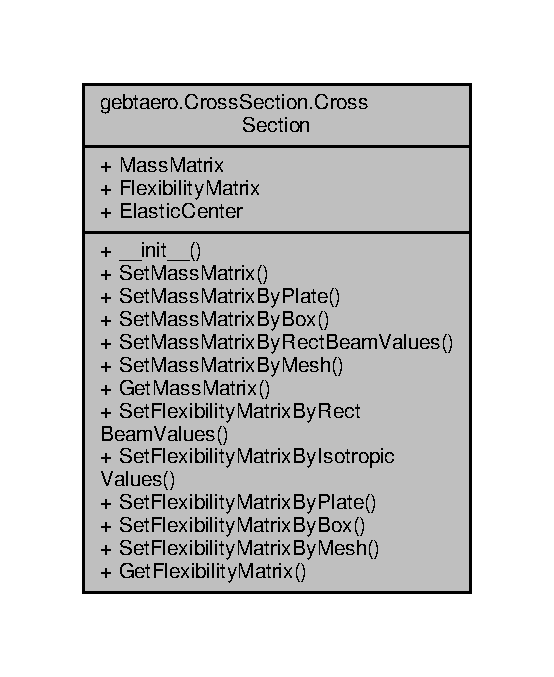
\includegraphics[width=266pt]{classgebtaero_1_1_cross_section_1_1_cross_section__coll__graph}
\end{center}
\end{figure}
\subsection*{Public Member Functions}
\begin{DoxyCompactItemize}
\item 
def \hyperlink{classgebtaero_1_1_cross_section_1_1_cross_section_a26142f8a77b098b8725d7d024cfd5199}{\+\_\+\+\_\+init\+\_\+\+\_\+} (self)
\begin{DoxyCompactList}\small\item\em The constructor initialize both matrices to zero. \end{DoxyCompactList}\item 
def \hyperlink{classgebtaero_1_1_cross_section_1_1_cross_section_a09866889e6a297e305d32daa5d57e1cb}{Set\+Mass\+Matrix} (self, Mu, I22, I33, I23, Nu, Zcg=0.)
\begin{DoxyCompactList}\small\item\em Set the Mass matrix using classical isotropic test cases parameters. \end{DoxyCompactList}\item 
def \hyperlink{classgebtaero_1_1_cross_section_1_1_cross_section_a0e87dd20eeef95c96cbbeebc0491fe86}{Set\+Mass\+Matrix\+By\+Plate} (self, Plate)
\begin{DoxyCompactList}\small\item\em Interface to \hyperlink{classgebtaero_1_1_composite_plate_1_1_composite_plate_a13b1222bb715056417c9db9903d264a2}{Composite\+Plate\+::\+Compute\+Mass\+Matrix}. \end{DoxyCompactList}\item 
def \hyperlink{classgebtaero_1_1_cross_section_1_1_cross_section_a4914caf35d9b8cfadafe8e359a590d7c}{Set\+Mass\+Matrix\+By\+Box} (self, Box)
\begin{DoxyCompactList}\small\item\em Interface to \hyperlink{classgebtaero_1_1_composite_box_1_1_composite_box_a6b944eeef7002377d7b83c5dd6ae6550}{Composite\+Box\+::\+Compute\+Mass\+Matrix}. \end{DoxyCompactList}\item 
def \hyperlink{classgebtaero_1_1_cross_section_1_1_cross_section_a7fa57a9ed49c1029409a78f45a45c562}{Set\+Mass\+Matrix\+By\+Rect\+Beam\+Values} (self, h, L, Mat, Neglect\+I22=False)
\begin{DoxyCompactList}\small\item\em Analytical definition of the \hyperlink{classgebtaero_1_1_cross_section_1_1_cross_section_ae9be8649853163b2b4dfdaa3584d9f78}{Cross\+Section\+::\+Mass\+Matrix} in case of a rectangular section isotropic beam. \end{DoxyCompactList}\item 
def \hyperlink{classgebtaero_1_1_cross_section_1_1_cross_section_a51f5f560da9f747310ebc55db72fd353}{Set\+Mass\+Matrix\+By\+Mesh} (self, Mesh, At\+Elastic\+Center=False, SymY=False, Chord\+Scale=False, verbosity=0)
\begin{DoxyCompactList}\small\item\em Interface to Mesh\+::\+Compute\+Mass\+Matrix\+From\+Mesh. \end{DoxyCompactList}\item 
def \hyperlink{classgebtaero_1_1_cross_section_1_1_cross_section_a329e4ccf313b33bf8fd5a1af65d95d0f}{Get\+Mass\+Matrix} (self)
\item 
def \hyperlink{classgebtaero_1_1_cross_section_1_1_cross_section_ae470ab0c1773947882a762c5e36351d5}{Set\+Flexibility\+Matrix\+By\+Rect\+Beam\+Values} (self, h, L, Mat, Rigid\+E\+Ig3=False)
\begin{DoxyCompactList}\small\item\em Analytical definition of the \hyperlink{classgebtaero_1_1_cross_section_1_1_cross_section_ac20eafaf38ff757f9a8c9ae89212396a}{Cross\+Section\+::\+Flexibility\+Matrix} for a rectangular section isotropic beam. \end{DoxyCompactList}\item 
def \hyperlink{classgebtaero_1_1_cross_section_1_1_cross_section_a8e1902ba4dd5fbdb184868b55b663ebc}{Set\+Flexibility\+Matrix\+By\+Isotropic\+Values} (self, E\+Ig2, E\+Ig3, GJ)
\begin{DoxyCompactList}\small\item\em Set the \hyperlink{classgebtaero_1_1_cross_section_1_1_cross_section_ac20eafaf38ff757f9a8c9ae89212396a}{Cross\+Section\+::\+Flexibility\+Matrix} using isotropic beam stiffness values. \end{DoxyCompactList}\item 
def \hyperlink{classgebtaero_1_1_cross_section_1_1_cross_section_a1f7fe7afe016bebd24eb42a7199df862}{Set\+Flexibility\+Matrix\+By\+Plate} (self, Plate, Type\+Elem, Nb\+ElemX, Nb\+ElemY, Nb\+Elem\+Ply, RigidX=False, RigidZ=False)
\begin{DoxyCompactList}\small\item\em Set the \hyperlink{classgebtaero_1_1_cross_section_1_1_cross_section_ac20eafaf38ff757f9a8c9ae89212396a}{Cross\+Section\+::\+Flexibility\+Matrix} using a periodic 3\+D\+F\+EM calculation with a \hyperlink{namespacegebtaero_1_1_composite_plate}{Composite\+Plate}. \end{DoxyCompactList}\item 
def \hyperlink{classgebtaero_1_1_cross_section_1_1_cross_section_ac316b6aa8955415debcc2f5dd6e28db6}{Set\+Flexibility\+Matrix\+By\+Box} (self, Box, Type\+Elem, Nb\+ElemX, Nb\+Elem\+YZ, Nb\+Elem\+Ply, RigidX=False, RigidZ=False)
\begin{DoxyCompactList}\small\item\em Set the \hyperlink{classgebtaero_1_1_cross_section_1_1_cross_section_ac20eafaf38ff757f9a8c9ae89212396a}{Cross\+Section\+::\+Flexibility\+Matrix} using a periodic 3\+D\+F\+EM calculation with a \hyperlink{namespacegebtaero_1_1_composite_box}{Composite\+Box}. \end{DoxyCompactList}\item 
def \hyperlink{classgebtaero_1_1_cross_section_1_1_cross_section_a70eb1851ddf4a3f88fb14cfc827e0c83}{Set\+Flexibility\+Matrix\+By\+Mesh} (self, Mesh, Plane\+Section=False, At\+Elastic\+Center=False, RigidX=False, RigidZ=False, Chord\+Scale=False)
\begin{DoxyCompactList}\small\item\em Set the \hyperlink{classgebtaero_1_1_cross_section_1_1_cross_section_ac20eafaf38ff757f9a8c9ae89212396a}{Cross\+Section\+::\+Flexibility\+Matrix} using Mesh. \end{DoxyCompactList}\item 
def \hyperlink{classgebtaero_1_1_cross_section_1_1_cross_section_ac06cec90003112b1de53b100c0085842}{Get\+Flexibility\+Matrix} (self)
\end{DoxyCompactItemize}
\subsection*{Public Attributes}
\begin{DoxyCompactItemize}
\item 
\hyperlink{classgebtaero_1_1_cross_section_1_1_cross_section_ae9be8649853163b2b4dfdaa3584d9f78}{Mass\+Matrix}
\begin{DoxyCompactList}\small\item\em Mass matrix of the cross section (see G\+E\+B\+T\+Aero paper) \end{DoxyCompactList}\item 
\hyperlink{classgebtaero_1_1_cross_section_1_1_cross_section_ac20eafaf38ff757f9a8c9ae89212396a}{Flexibility\+Matrix}
\begin{DoxyCompactList}\small\item\em Flexibility matrix of the cross section (see G\+E\+B\+T\+Aero paper) \end{DoxyCompactList}\item 
\hyperlink{classgebtaero_1_1_cross_section_1_1_cross_section_a1eb436d0de5edf2c25612bbc15d88d91}{Elastic\+Center}
\begin{DoxyCompactList}\small\item\em Coordinate of the elastic center in the plane (yB,Zb) \end{DoxyCompactList}\end{DoxyCompactItemize}


\subsection{Detailed Description}
This class is used to determine the Mass matrix and the flexibility matrix of a cross section. 

It could be done analytically or with the 3D F\+EM solver ccx. 

Definition at line 7 of file Cross\+Section.\+py.



\subsection{Constructor \& Destructor Documentation}
\mbox{\Hypertarget{classgebtaero_1_1_cross_section_1_1_cross_section_a26142f8a77b098b8725d7d024cfd5199}\label{classgebtaero_1_1_cross_section_1_1_cross_section_a26142f8a77b098b8725d7d024cfd5199}} 
\index{gebtaero\+::\+Cross\+Section\+::\+Cross\+Section@{gebtaero\+::\+Cross\+Section\+::\+Cross\+Section}!\+\_\+\+\_\+init\+\_\+\+\_\+@{\+\_\+\+\_\+init\+\_\+\+\_\+}}
\index{\+\_\+\+\_\+init\+\_\+\+\_\+@{\+\_\+\+\_\+init\+\_\+\+\_\+}!gebtaero\+::\+Cross\+Section\+::\+Cross\+Section@{gebtaero\+::\+Cross\+Section\+::\+Cross\+Section}}
\subsubsection{\texorpdfstring{\+\_\+\+\_\+init\+\_\+\+\_\+()}{\_\_init\_\_()}}
{\footnotesize\ttfamily def gebtaero.\+Cross\+Section.\+Cross\+Section.\+\_\+\+\_\+init\+\_\+\+\_\+ (\begin{DoxyParamCaption}\item[{}]{self }\end{DoxyParamCaption})}



The constructor initialize both matrices to zero. 



Definition at line 10 of file Cross\+Section.\+py.



\subsection{Member Function Documentation}
\mbox{\Hypertarget{classgebtaero_1_1_cross_section_1_1_cross_section_ac06cec90003112b1de53b100c0085842}\label{classgebtaero_1_1_cross_section_1_1_cross_section_ac06cec90003112b1de53b100c0085842}} 
\index{gebtaero\+::\+Cross\+Section\+::\+Cross\+Section@{gebtaero\+::\+Cross\+Section\+::\+Cross\+Section}!Get\+Flexibility\+Matrix@{Get\+Flexibility\+Matrix}}
\index{Get\+Flexibility\+Matrix@{Get\+Flexibility\+Matrix}!gebtaero\+::\+Cross\+Section\+::\+Cross\+Section@{gebtaero\+::\+Cross\+Section\+::\+Cross\+Section}}
\subsubsection{\texorpdfstring{Get\+Flexibility\+Matrix()}{GetFlexibilityMatrix()}}
{\footnotesize\ttfamily def gebtaero.\+Cross\+Section.\+Cross\+Section.\+Get\+Flexibility\+Matrix (\begin{DoxyParamCaption}\item[{}]{self }\end{DoxyParamCaption})}



Definition at line 244 of file Cross\+Section.\+py.

\mbox{\Hypertarget{classgebtaero_1_1_cross_section_1_1_cross_section_a329e4ccf313b33bf8fd5a1af65d95d0f}\label{classgebtaero_1_1_cross_section_1_1_cross_section_a329e4ccf313b33bf8fd5a1af65d95d0f}} 
\index{gebtaero\+::\+Cross\+Section\+::\+Cross\+Section@{gebtaero\+::\+Cross\+Section\+::\+Cross\+Section}!Get\+Mass\+Matrix@{Get\+Mass\+Matrix}}
\index{Get\+Mass\+Matrix@{Get\+Mass\+Matrix}!gebtaero\+::\+Cross\+Section\+::\+Cross\+Section@{gebtaero\+::\+Cross\+Section\+::\+Cross\+Section}}
\subsubsection{\texorpdfstring{Get\+Mass\+Matrix()}{GetMassMatrix()}}
{\footnotesize\ttfamily def gebtaero.\+Cross\+Section.\+Cross\+Section.\+Get\+Mass\+Matrix (\begin{DoxyParamCaption}\item[{}]{self }\end{DoxyParamCaption})}



Definition at line 117 of file Cross\+Section.\+py.

\mbox{\Hypertarget{classgebtaero_1_1_cross_section_1_1_cross_section_ac316b6aa8955415debcc2f5dd6e28db6}\label{classgebtaero_1_1_cross_section_1_1_cross_section_ac316b6aa8955415debcc2f5dd6e28db6}} 
\index{gebtaero\+::\+Cross\+Section\+::\+Cross\+Section@{gebtaero\+::\+Cross\+Section\+::\+Cross\+Section}!Set\+Flexibility\+Matrix\+By\+Box@{Set\+Flexibility\+Matrix\+By\+Box}}
\index{Set\+Flexibility\+Matrix\+By\+Box@{Set\+Flexibility\+Matrix\+By\+Box}!gebtaero\+::\+Cross\+Section\+::\+Cross\+Section@{gebtaero\+::\+Cross\+Section\+::\+Cross\+Section}}
\subsubsection{\texorpdfstring{Set\+Flexibility\+Matrix\+By\+Box()}{SetFlexibilityMatrixByBox()}}
{\footnotesize\ttfamily def gebtaero.\+Cross\+Section.\+Cross\+Section.\+Set\+Flexibility\+Matrix\+By\+Box (\begin{DoxyParamCaption}\item[{}]{self,  }\item[{}]{Box,  }\item[{}]{Type\+Elem,  }\item[{}]{Nb\+ElemX,  }\item[{}]{Nb\+Elem\+YZ,  }\item[{}]{Nb\+Elem\+Ply,  }\item[{}]{RigidX = {\ttfamily False},  }\item[{}]{RigidZ = {\ttfamily False} }\end{DoxyParamCaption})}



Set the \hyperlink{classgebtaero_1_1_cross_section_1_1_cross_section_ac20eafaf38ff757f9a8c9ae89212396a}{Cross\+Section\+::\+Flexibility\+Matrix} using a periodic 3\+D\+F\+EM calculation with a \hyperlink{namespacegebtaero_1_1_composite_box}{Composite\+Box}. 


\begin{DoxyParams}{Parameters}
{\em Box} & the \hyperlink{namespacegebtaero_1_1_composite_box}{Composite\+Box} used for the calculation \\
\hline
{\em Type\+Elem} & the type of finite element used for the computation. Supported \+: he20r, he20, he8i, he8, pe15 (see ccx doc) \\
\hline
{\em Nb\+ElemX} & the number of finite element across the beam direction (for a constant cross section, 1 element is enough) \\
\hline
{\em N\+B\+Elem\+YZ} & the number of finite element along the wall directions \\
\hline
{\em N\+B\+Elem\+Ply} & the number of finite element in a composite ply \\
\hline
{\em RigidX} & True = supress the traction ddl of the beam \\
\hline
{\em RigidZ} & True = supress the bending in the lag axis ddl \\
\hline
\end{DoxyParams}


Definition at line 195 of file Cross\+Section.\+py.

\mbox{\Hypertarget{classgebtaero_1_1_cross_section_1_1_cross_section_a8e1902ba4dd5fbdb184868b55b663ebc}\label{classgebtaero_1_1_cross_section_1_1_cross_section_a8e1902ba4dd5fbdb184868b55b663ebc}} 
\index{gebtaero\+::\+Cross\+Section\+::\+Cross\+Section@{gebtaero\+::\+Cross\+Section\+::\+Cross\+Section}!Set\+Flexibility\+Matrix\+By\+Isotropic\+Values@{Set\+Flexibility\+Matrix\+By\+Isotropic\+Values}}
\index{Set\+Flexibility\+Matrix\+By\+Isotropic\+Values@{Set\+Flexibility\+Matrix\+By\+Isotropic\+Values}!gebtaero\+::\+Cross\+Section\+::\+Cross\+Section@{gebtaero\+::\+Cross\+Section\+::\+Cross\+Section}}
\subsubsection{\texorpdfstring{Set\+Flexibility\+Matrix\+By\+Isotropic\+Values()}{SetFlexibilityMatrixByIsotropicValues()}}
{\footnotesize\ttfamily def gebtaero.\+Cross\+Section.\+Cross\+Section.\+Set\+Flexibility\+Matrix\+By\+Isotropic\+Values (\begin{DoxyParamCaption}\item[{}]{self,  }\item[{}]{E\+Ig2,  }\item[{}]{E\+Ig3,  }\item[{}]{GJ }\end{DoxyParamCaption})}



Set the \hyperlink{classgebtaero_1_1_cross_section_1_1_cross_section_ac20eafaf38ff757f9a8c9ae89212396a}{Cross\+Section\+::\+Flexibility\+Matrix} using isotropic beam stiffness values. 


\begin{DoxyParams}{Parameters}
{\em E\+Ig2} & bending stiffness span-\/wise \\
\hline
{\em E\+Ig3} & bending stiffness chord-\/wise \\
\hline
{\em GJ} & torsional stiffness \\
\hline
\end{DoxyParams}


Definition at line 147 of file Cross\+Section.\+py.

Here is the caller graph for this function\+:\nopagebreak
\begin{figure}[H]
\begin{center}
\leavevmode
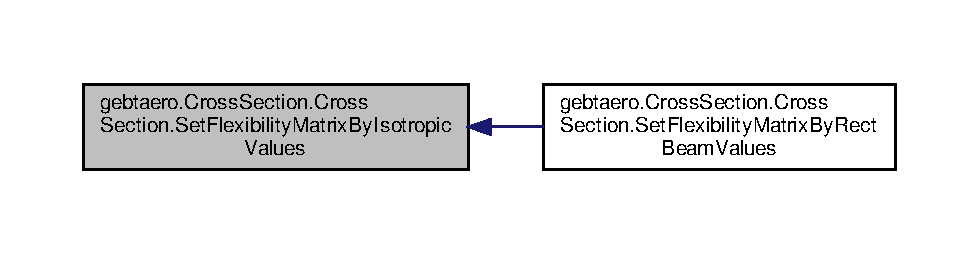
\includegraphics[width=350pt]{classgebtaero_1_1_cross_section_1_1_cross_section_a8e1902ba4dd5fbdb184868b55b663ebc_icgraph}
\end{center}
\end{figure}
\mbox{\Hypertarget{classgebtaero_1_1_cross_section_1_1_cross_section_a70eb1851ddf4a3f88fb14cfc827e0c83}\label{classgebtaero_1_1_cross_section_1_1_cross_section_a70eb1851ddf4a3f88fb14cfc827e0c83}} 
\index{gebtaero\+::\+Cross\+Section\+::\+Cross\+Section@{gebtaero\+::\+Cross\+Section\+::\+Cross\+Section}!Set\+Flexibility\+Matrix\+By\+Mesh@{Set\+Flexibility\+Matrix\+By\+Mesh}}
\index{Set\+Flexibility\+Matrix\+By\+Mesh@{Set\+Flexibility\+Matrix\+By\+Mesh}!gebtaero\+::\+Cross\+Section\+::\+Cross\+Section@{gebtaero\+::\+Cross\+Section\+::\+Cross\+Section}}
\subsubsection{\texorpdfstring{Set\+Flexibility\+Matrix\+By\+Mesh()}{SetFlexibilityMatrixByMesh()}}
{\footnotesize\ttfamily def gebtaero.\+Cross\+Section.\+Cross\+Section.\+Set\+Flexibility\+Matrix\+By\+Mesh (\begin{DoxyParamCaption}\item[{}]{self,  }\item[{}]{Mesh,  }\item[{}]{Plane\+Section = {\ttfamily False},  }\item[{}]{At\+Elastic\+Center = {\ttfamily False},  }\item[{}]{RigidX = {\ttfamily False},  }\item[{}]{RigidZ = {\ttfamily False},  }\item[{}]{Chord\+Scale = {\ttfamily False} }\end{DoxyParamCaption})}



Set the \hyperlink{classgebtaero_1_1_cross_section_1_1_cross_section_ac20eafaf38ff757f9a8c9ae89212396a}{Cross\+Section\+::\+Flexibility\+Matrix} using Mesh. 


\begin{DoxyParams}{Parameters}
{\em Mesh} & The Mesh used for the calculation (inp format) \\
\hline
{\em Plane\+Section} & True = warping of the cross section is not allowed, False = warping of the cross section is allowed \\
\hline
{\em At\+Elastic\+Center} & Compute the Elastic center and then compute the mass matrix at the elastic center \\
\hline
{\em RigidX} & True = supress the traction ddl of the beam \\
\hline
{\em RigidZ} & True = supress the bending in the lag axis ddl \\
\hline
{\em Chord\+Scale} & True = the Mesh have a dimension 1 in the chord direction (yB) the mass matrix obtained is scaled afterward with the parameter Mesh\+::\+Chord \\
\hline
\end{DoxyParams}


Definition at line 218 of file Cross\+Section.\+py.

\mbox{\Hypertarget{classgebtaero_1_1_cross_section_1_1_cross_section_a1f7fe7afe016bebd24eb42a7199df862}\label{classgebtaero_1_1_cross_section_1_1_cross_section_a1f7fe7afe016bebd24eb42a7199df862}} 
\index{gebtaero\+::\+Cross\+Section\+::\+Cross\+Section@{gebtaero\+::\+Cross\+Section\+::\+Cross\+Section}!Set\+Flexibility\+Matrix\+By\+Plate@{Set\+Flexibility\+Matrix\+By\+Plate}}
\index{Set\+Flexibility\+Matrix\+By\+Plate@{Set\+Flexibility\+Matrix\+By\+Plate}!gebtaero\+::\+Cross\+Section\+::\+Cross\+Section@{gebtaero\+::\+Cross\+Section\+::\+Cross\+Section}}
\subsubsection{\texorpdfstring{Set\+Flexibility\+Matrix\+By\+Plate()}{SetFlexibilityMatrixByPlate()}}
{\footnotesize\ttfamily def gebtaero.\+Cross\+Section.\+Cross\+Section.\+Set\+Flexibility\+Matrix\+By\+Plate (\begin{DoxyParamCaption}\item[{}]{self,  }\item[{}]{Plate,  }\item[{}]{Type\+Elem,  }\item[{}]{Nb\+ElemX,  }\item[{}]{Nb\+ElemY,  }\item[{}]{Nb\+Elem\+Ply,  }\item[{}]{RigidX = {\ttfamily False},  }\item[{}]{RigidZ = {\ttfamily False} }\end{DoxyParamCaption})}



Set the \hyperlink{classgebtaero_1_1_cross_section_1_1_cross_section_ac20eafaf38ff757f9a8c9ae89212396a}{Cross\+Section\+::\+Flexibility\+Matrix} using a periodic 3\+D\+F\+EM calculation with a \hyperlink{namespacegebtaero_1_1_composite_plate}{Composite\+Plate}. 


\begin{DoxyParams}{Parameters}
{\em Plate} & the \hyperlink{namespacegebtaero_1_1_composite_plate}{Composite\+Plate} used for the calculation \\
\hline
{\em Type\+Elem} & the type of finite element used for the computation. Supported \+: he20r, he20, he8i, he8, pe15 (see ccx doc) \\
\hline
{\em Nb\+ElemX} & the number of finite element across the beam direction (for a constant cross section, 1 element is enough) \\
\hline
{\em N\+B\+ElemY} & the number of finite element across the width \\
\hline
{\em N\+B\+Elem\+Ply} & the number of finite element in a composite ply \\
\hline
{\em RigidX} & True = supress the traction ddl of the beam \\
\hline
{\em RigidZ} & True = supress the bending in the lag axis ddl \\
\hline
\end{DoxyParams}


Definition at line 171 of file Cross\+Section.\+py.

\mbox{\Hypertarget{classgebtaero_1_1_cross_section_1_1_cross_section_ae470ab0c1773947882a762c5e36351d5}\label{classgebtaero_1_1_cross_section_1_1_cross_section_ae470ab0c1773947882a762c5e36351d5}} 
\index{gebtaero\+::\+Cross\+Section\+::\+Cross\+Section@{gebtaero\+::\+Cross\+Section\+::\+Cross\+Section}!Set\+Flexibility\+Matrix\+By\+Rect\+Beam\+Values@{Set\+Flexibility\+Matrix\+By\+Rect\+Beam\+Values}}
\index{Set\+Flexibility\+Matrix\+By\+Rect\+Beam\+Values@{Set\+Flexibility\+Matrix\+By\+Rect\+Beam\+Values}!gebtaero\+::\+Cross\+Section\+::\+Cross\+Section@{gebtaero\+::\+Cross\+Section\+::\+Cross\+Section}}
\subsubsection{\texorpdfstring{Set\+Flexibility\+Matrix\+By\+Rect\+Beam\+Values()}{SetFlexibilityMatrixByRectBeamValues()}}
{\footnotesize\ttfamily def gebtaero.\+Cross\+Section.\+Cross\+Section.\+Set\+Flexibility\+Matrix\+By\+Rect\+Beam\+Values (\begin{DoxyParamCaption}\item[{}]{self,  }\item[{}]{h,  }\item[{}]{L,  }\item[{}]{Mat,  }\item[{}]{Rigid\+E\+Ig3 = {\ttfamily False} }\end{DoxyParamCaption})}



Analytical definition of the \hyperlink{classgebtaero_1_1_cross_section_1_1_cross_section_ac20eafaf38ff757f9a8c9ae89212396a}{Cross\+Section\+::\+Flexibility\+Matrix} for a rectangular section isotropic beam. 


\begin{DoxyParams}{Parameters}
{\em h} & Section height \\
\hline
{\em L} & Section width \\
\hline
{\em Mat} & Material of the beam (must be \hyperlink{namespacegebtaero_1_1_iso_material}{Iso\+Material}) \\
\hline
{\em Rigid\+E\+Ig3} & True = supress the bending ddl in the lag axis \\
\hline
\end{DoxyParams}


Definition at line 125 of file Cross\+Section.\+py.

\mbox{\Hypertarget{classgebtaero_1_1_cross_section_1_1_cross_section_a09866889e6a297e305d32daa5d57e1cb}\label{classgebtaero_1_1_cross_section_1_1_cross_section_a09866889e6a297e305d32daa5d57e1cb}} 
\index{gebtaero\+::\+Cross\+Section\+::\+Cross\+Section@{gebtaero\+::\+Cross\+Section\+::\+Cross\+Section}!Set\+Mass\+Matrix@{Set\+Mass\+Matrix}}
\index{Set\+Mass\+Matrix@{Set\+Mass\+Matrix}!gebtaero\+::\+Cross\+Section\+::\+Cross\+Section@{gebtaero\+::\+Cross\+Section\+::\+Cross\+Section}}
\subsubsection{\texorpdfstring{Set\+Mass\+Matrix()}{SetMassMatrix()}}
{\footnotesize\ttfamily def gebtaero.\+Cross\+Section.\+Cross\+Section.\+Set\+Mass\+Matrix (\begin{DoxyParamCaption}\item[{}]{self,  }\item[{}]{Mu,  }\item[{}]{I22,  }\item[{}]{I33,  }\item[{}]{I23,  }\item[{}]{Nu,  }\item[{}]{Zcg = {\ttfamily 0.} }\end{DoxyParamCaption})}



Set the Mass matrix using classical isotropic test cases parameters. 


\begin{DoxyParams}{Parameters}
{\em Mu} & Mass per unit length (kg/m) \\
\hline
{\em I22} & mass moment of inertia around yB (bending span-\/wise, kg.\+m) \\
\hline
{\em I33} & mass moment of inertia around zB (bending chord-\/wise, kg.\+m) \\
\hline
{\em I23} & product of inertia in plane (yB,zB) \\
\hline
{\em Nu} & \+: Distance between moment calculation point and center of gravity. Positif is the CG is near leading edge \\
\hline
{\em Zcg} & \+: coordinate Z of the center of gravity in frame B \\
\hline
\end{DoxyParams}


Definition at line 25 of file Cross\+Section.\+py.

Here is the caller graph for this function\+:\nopagebreak
\begin{figure}[H]
\begin{center}
\leavevmode
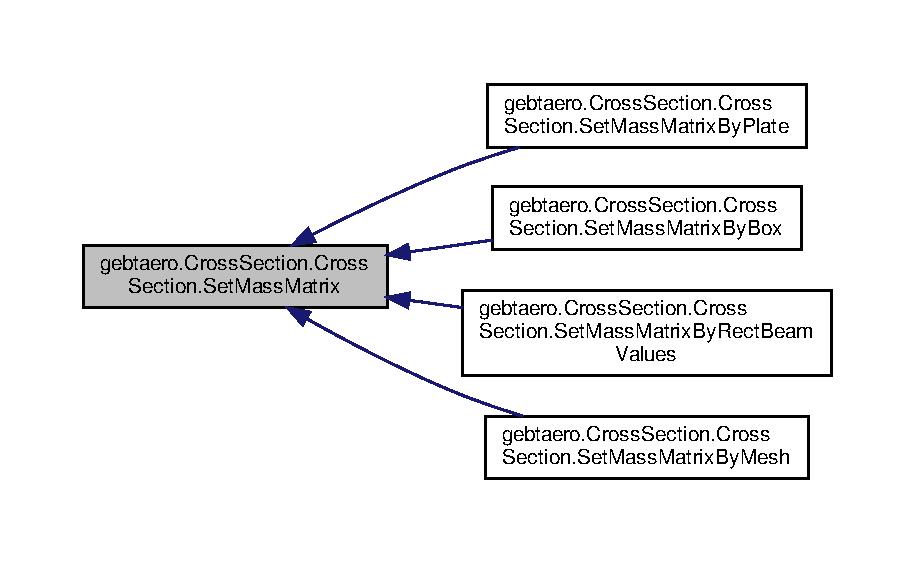
\includegraphics[width=350pt]{classgebtaero_1_1_cross_section_1_1_cross_section_a09866889e6a297e305d32daa5d57e1cb_icgraph}
\end{center}
\end{figure}
\mbox{\Hypertarget{classgebtaero_1_1_cross_section_1_1_cross_section_a4914caf35d9b8cfadafe8e359a590d7c}\label{classgebtaero_1_1_cross_section_1_1_cross_section_a4914caf35d9b8cfadafe8e359a590d7c}} 
\index{gebtaero\+::\+Cross\+Section\+::\+Cross\+Section@{gebtaero\+::\+Cross\+Section\+::\+Cross\+Section}!Set\+Mass\+Matrix\+By\+Box@{Set\+Mass\+Matrix\+By\+Box}}
\index{Set\+Mass\+Matrix\+By\+Box@{Set\+Mass\+Matrix\+By\+Box}!gebtaero\+::\+Cross\+Section\+::\+Cross\+Section@{gebtaero\+::\+Cross\+Section\+::\+Cross\+Section}}
\subsubsection{\texorpdfstring{Set\+Mass\+Matrix\+By\+Box()}{SetMassMatrixByBox()}}
{\footnotesize\ttfamily def gebtaero.\+Cross\+Section.\+Cross\+Section.\+Set\+Mass\+Matrix\+By\+Box (\begin{DoxyParamCaption}\item[{}]{self,  }\item[{}]{Box }\end{DoxyParamCaption})}



Interface to \hyperlink{classgebtaero_1_1_composite_box_1_1_composite_box_a6b944eeef7002377d7b83c5dd6ae6550}{Composite\+Box\+::\+Compute\+Mass\+Matrix}. 



Definition at line 51 of file Cross\+Section.\+py.

\mbox{\Hypertarget{classgebtaero_1_1_cross_section_1_1_cross_section_a51f5f560da9f747310ebc55db72fd353}\label{classgebtaero_1_1_cross_section_1_1_cross_section_a51f5f560da9f747310ebc55db72fd353}} 
\index{gebtaero\+::\+Cross\+Section\+::\+Cross\+Section@{gebtaero\+::\+Cross\+Section\+::\+Cross\+Section}!Set\+Mass\+Matrix\+By\+Mesh@{Set\+Mass\+Matrix\+By\+Mesh}}
\index{Set\+Mass\+Matrix\+By\+Mesh@{Set\+Mass\+Matrix\+By\+Mesh}!gebtaero\+::\+Cross\+Section\+::\+Cross\+Section@{gebtaero\+::\+Cross\+Section\+::\+Cross\+Section}}
\subsubsection{\texorpdfstring{Set\+Mass\+Matrix\+By\+Mesh()}{SetMassMatrixByMesh()}}
{\footnotesize\ttfamily def gebtaero.\+Cross\+Section.\+Cross\+Section.\+Set\+Mass\+Matrix\+By\+Mesh (\begin{DoxyParamCaption}\item[{}]{self,  }\item[{}]{Mesh,  }\item[{}]{At\+Elastic\+Center = {\ttfamily False},  }\item[{}]{SymY = {\ttfamily False},  }\item[{}]{Chord\+Scale = {\ttfamily False},  }\item[{}]{verbosity = {\ttfamily 0} }\end{DoxyParamCaption})}



Interface to Mesh\+::\+Compute\+Mass\+Matrix\+From\+Mesh. 


\begin{DoxyParams}{Parameters}
{\em Mesh} & The Mesh used for the calculation (inp format) \\
\hline
{\em At\+Elastic\+Center} & Compute the Elastic center and then compute the mass matrix at the elastic center \\
\hline
{\em SymY} & True = force the horizontal symetry of the cross section \\
\hline
{\em Chord\+Scale} & True = the Mesh have a dimension 1 in the chord direction (yB) the mass matrix obtained is scaled afterward with the parameter Mesh\+::\+Chord \\
\hline
{\em verbosity} & 0 = no log, 1 = output the log of the computation \\
\hline
\end{DoxyParams}


Definition at line 81 of file Cross\+Section.\+py.

\mbox{\Hypertarget{classgebtaero_1_1_cross_section_1_1_cross_section_a0e87dd20eeef95c96cbbeebc0491fe86}\label{classgebtaero_1_1_cross_section_1_1_cross_section_a0e87dd20eeef95c96cbbeebc0491fe86}} 
\index{gebtaero\+::\+Cross\+Section\+::\+Cross\+Section@{gebtaero\+::\+Cross\+Section\+::\+Cross\+Section}!Set\+Mass\+Matrix\+By\+Plate@{Set\+Mass\+Matrix\+By\+Plate}}
\index{Set\+Mass\+Matrix\+By\+Plate@{Set\+Mass\+Matrix\+By\+Plate}!gebtaero\+::\+Cross\+Section\+::\+Cross\+Section@{gebtaero\+::\+Cross\+Section\+::\+Cross\+Section}}
\subsubsection{\texorpdfstring{Set\+Mass\+Matrix\+By\+Plate()}{SetMassMatrixByPlate()}}
{\footnotesize\ttfamily def gebtaero.\+Cross\+Section.\+Cross\+Section.\+Set\+Mass\+Matrix\+By\+Plate (\begin{DoxyParamCaption}\item[{}]{self,  }\item[{}]{Plate }\end{DoxyParamCaption})}



Interface to \hyperlink{classgebtaero_1_1_composite_plate_1_1_composite_plate_a13b1222bb715056417c9db9903d264a2}{Composite\+Plate\+::\+Compute\+Mass\+Matrix}. 



Definition at line 45 of file Cross\+Section.\+py.

\mbox{\Hypertarget{classgebtaero_1_1_cross_section_1_1_cross_section_a7fa57a9ed49c1029409a78f45a45c562}\label{classgebtaero_1_1_cross_section_1_1_cross_section_a7fa57a9ed49c1029409a78f45a45c562}} 
\index{gebtaero\+::\+Cross\+Section\+::\+Cross\+Section@{gebtaero\+::\+Cross\+Section\+::\+Cross\+Section}!Set\+Mass\+Matrix\+By\+Rect\+Beam\+Values@{Set\+Mass\+Matrix\+By\+Rect\+Beam\+Values}}
\index{Set\+Mass\+Matrix\+By\+Rect\+Beam\+Values@{Set\+Mass\+Matrix\+By\+Rect\+Beam\+Values}!gebtaero\+::\+Cross\+Section\+::\+Cross\+Section@{gebtaero\+::\+Cross\+Section\+::\+Cross\+Section}}
\subsubsection{\texorpdfstring{Set\+Mass\+Matrix\+By\+Rect\+Beam\+Values()}{SetMassMatrixByRectBeamValues()}}
{\footnotesize\ttfamily def gebtaero.\+Cross\+Section.\+Cross\+Section.\+Set\+Mass\+Matrix\+By\+Rect\+Beam\+Values (\begin{DoxyParamCaption}\item[{}]{self,  }\item[{}]{h,  }\item[{}]{L,  }\item[{}]{Mat,  }\item[{}]{Neglect\+I22 = {\ttfamily False} }\end{DoxyParamCaption})}



Analytical definition of the \hyperlink{classgebtaero_1_1_cross_section_1_1_cross_section_ae9be8649853163b2b4dfdaa3584d9f78}{Cross\+Section\+::\+Mass\+Matrix} in case of a rectangular section isotropic beam. 


\begin{DoxyParams}{Parameters}
{\em h} & Section height \\
\hline
{\em L} & Section width \\
\hline
{\em Mat} & Material of the beam (must be \hyperlink{namespacegebtaero_1_1_iso_material}{Iso\+Material}) \\
\hline
{\em Neglect\+I22} & True = the value of I22 is forced to zero, False = nothing appends \\
\hline
\end{DoxyParams}


Definition at line 61 of file Cross\+Section.\+py.



\subsection{Member Data Documentation}
\mbox{\Hypertarget{classgebtaero_1_1_cross_section_1_1_cross_section_a1eb436d0de5edf2c25612bbc15d88d91}\label{classgebtaero_1_1_cross_section_1_1_cross_section_a1eb436d0de5edf2c25612bbc15d88d91}} 
\index{gebtaero\+::\+Cross\+Section\+::\+Cross\+Section@{gebtaero\+::\+Cross\+Section\+::\+Cross\+Section}!Elastic\+Center@{Elastic\+Center}}
\index{Elastic\+Center@{Elastic\+Center}!gebtaero\+::\+Cross\+Section\+::\+Cross\+Section@{gebtaero\+::\+Cross\+Section\+::\+Cross\+Section}}
\subsubsection{\texorpdfstring{Elastic\+Center}{ElasticCenter}}
{\footnotesize\ttfamily gebtaero.\+Cross\+Section.\+Cross\+Section.\+Elastic\+Center}



Coordinate of the elastic center in the plane (yB,Zb) 



Definition at line 16 of file Cross\+Section.\+py.

\mbox{\Hypertarget{classgebtaero_1_1_cross_section_1_1_cross_section_ac20eafaf38ff757f9a8c9ae89212396a}\label{classgebtaero_1_1_cross_section_1_1_cross_section_ac20eafaf38ff757f9a8c9ae89212396a}} 
\index{gebtaero\+::\+Cross\+Section\+::\+Cross\+Section@{gebtaero\+::\+Cross\+Section\+::\+Cross\+Section}!Flexibility\+Matrix@{Flexibility\+Matrix}}
\index{Flexibility\+Matrix@{Flexibility\+Matrix}!gebtaero\+::\+Cross\+Section\+::\+Cross\+Section@{gebtaero\+::\+Cross\+Section\+::\+Cross\+Section}}
\subsubsection{\texorpdfstring{Flexibility\+Matrix}{FlexibilityMatrix}}
{\footnotesize\ttfamily gebtaero.\+Cross\+Section.\+Cross\+Section.\+Flexibility\+Matrix}



Flexibility matrix of the cross section (see G\+E\+B\+T\+Aero paper) 



Definition at line 14 of file Cross\+Section.\+py.

\mbox{\Hypertarget{classgebtaero_1_1_cross_section_1_1_cross_section_ae9be8649853163b2b4dfdaa3584d9f78}\label{classgebtaero_1_1_cross_section_1_1_cross_section_ae9be8649853163b2b4dfdaa3584d9f78}} 
\index{gebtaero\+::\+Cross\+Section\+::\+Cross\+Section@{gebtaero\+::\+Cross\+Section\+::\+Cross\+Section}!Mass\+Matrix@{Mass\+Matrix}}
\index{Mass\+Matrix@{Mass\+Matrix}!gebtaero\+::\+Cross\+Section\+::\+Cross\+Section@{gebtaero\+::\+Cross\+Section\+::\+Cross\+Section}}
\subsubsection{\texorpdfstring{Mass\+Matrix}{MassMatrix}}
{\footnotesize\ttfamily gebtaero.\+Cross\+Section.\+Cross\+Section.\+Mass\+Matrix}



Mass matrix of the cross section (see G\+E\+B\+T\+Aero paper) 



Definition at line 12 of file Cross\+Section.\+py.



The documentation for this class was generated from the following file\+:\begin{DoxyCompactItemize}
\item 
/home/bertrand/logiciels/gebtaero\+\_\+frama/src/gebtaero/\hyperlink{_cross_section_8py}{Cross\+Section.\+py}\end{DoxyCompactItemize}

\hypertarget{structprescribedcondition_1_1distriload}{}\section{prescribedcondition\+:\+:distriload Type Reference}
\label{structprescribedcondition_1_1distriload}\index{prescribedcondition\+::distriload@{prescribedcondition\+::distriload}}


Define the distributed load condition.  


\subsection*{Private Attributes}
\begin{DoxyCompactItemize}
\item 
real(dbl), dimension(nstrn) \hyperlink{structprescribedcondition_1_1distriload_a32fb9fe519f0164a70313c8e7627976b}{value}
\begin{DoxyCompactList}\small\item\em the current functional value of the load \end{DoxyCompactList}\item 
real(dbl), dimension(nstrn, nstrn) \hyperlink{structprescribedcondition_1_1distriload_ac5734eaac28c08f44fd4f41857df75b2}{distr\+\_\+fun}
\begin{DoxyCompactList}\small\item\em the distribution function for each load \end{DoxyCompactList}\item 
integer, dimension(nstrn) \hyperlink{structprescribedcondition_1_1distriload_a476acfacfaac7a9d8ebaf6ce371279ff}{follower}
\begin{DoxyCompactList}\small\item\em whether the force vector/moment vector are follower quantities \end{DoxyCompactList}\end{DoxyCompactItemize}


\subsection{Detailed Description}
Define the distributed load condition. 

Definition at line 41 of file Prescribed\+Condition.\+f90.



\subsection{Member Data Documentation}
\mbox{\Hypertarget{structprescribedcondition_1_1distriload_ac5734eaac28c08f44fd4f41857df75b2}\label{structprescribedcondition_1_1distriload_ac5734eaac28c08f44fd4f41857df75b2}} 
\index{prescribedcondition\+::distriload@{prescribedcondition\+::distriload}!distr\+\_\+fun@{distr\+\_\+fun}}
\index{distr\+\_\+fun@{distr\+\_\+fun}!prescribedcondition\+::distriload@{prescribedcondition\+::distriload}}
\subsubsection{\texorpdfstring{distr\+\_\+fun}{distr\_fun}}
{\footnotesize\ttfamily real(dbl), dimension(nstrn,nstrn) prescribedcondition\+::distriload\+::distr\+\_\+fun\hspace{0.3cm}{\ttfamily [private]}}



the distribution function for each load 



Definition at line 44 of file Prescribed\+Condition.\+f90.

\mbox{\Hypertarget{structprescribedcondition_1_1distriload_a476acfacfaac7a9d8ebaf6ce371279ff}\label{structprescribedcondition_1_1distriload_a476acfacfaac7a9d8ebaf6ce371279ff}} 
\index{prescribedcondition\+::distriload@{prescribedcondition\+::distriload}!follower@{follower}}
\index{follower@{follower}!prescribedcondition\+::distriload@{prescribedcondition\+::distriload}}
\subsubsection{\texorpdfstring{follower}{follower}}
{\footnotesize\ttfamily integer, dimension(nstrn) prescribedcondition\+::distriload\+::follower\hspace{0.3cm}{\ttfamily [private]}}



whether the force vector/moment vector are follower quantities 



Definition at line 45 of file Prescribed\+Condition.\+f90.

\mbox{\Hypertarget{structprescribedcondition_1_1distriload_a32fb9fe519f0164a70313c8e7627976b}\label{structprescribedcondition_1_1distriload_a32fb9fe519f0164a70313c8e7627976b}} 
\index{prescribedcondition\+::distriload@{prescribedcondition\+::distriload}!value@{value}}
\index{value@{value}!prescribedcondition\+::distriload@{prescribedcondition\+::distriload}}
\subsubsection{\texorpdfstring{value}{value}}
{\footnotesize\ttfamily real(dbl), dimension(nstrn) prescribedcondition\+::distriload\+::value\hspace{0.3cm}{\ttfamily [private]}}



the current functional value of the load 



Definition at line 43 of file Prescribed\+Condition.\+f90.



The documentation for this type was generated from the following file\+:\begin{DoxyCompactItemize}
\item 
/home/bertrand/these/logiciels/programme/src/\hyperlink{_prescribed_condition_8f90}{Prescribed\+Condition.\+f90}\end{DoxyCompactItemize}

\hypertarget{classgebtaero_1_1_external_mesh_1_1_external_mesh}{}\section{gebtaero.\+External\+Mesh.\+External\+Mesh Class Reference}
\label{classgebtaero_1_1_external_mesh_1_1_external_mesh}\index{gebtaero.\+External\+Mesh.\+External\+Mesh@{gebtaero.\+External\+Mesh.\+External\+Mesh}}
\subsection*{Public Member Functions}
\begin{DoxyCompactItemize}
\item 
def \hyperlink{classgebtaero_1_1_external_mesh_1_1_external_mesh_ad1301073ba0c00d8ad8fe3dc4baa6068}{\+\_\+\+\_\+init\+\_\+\+\_\+} (self, \hyperlink{classgebtaero_1_1_external_mesh_1_1_external_mesh_a53b38c75b026fb6c56b50b2dd9b5270f}{Mesh\+File}, \hyperlink{classgebtaero_1_1_external_mesh_1_1_external_mesh_a87faefe634a474727d516e58eb8bf944}{OffsetY}=0., \hyperlink{classgebtaero_1_1_external_mesh_1_1_external_mesh_a6639038ee73b225cf0d3ea1bd9c52783}{OffsetZ}=0., Unv\+Conv=False, \hyperlink{classgebtaero_1_1_external_mesh_1_1_external_mesh_ac9f8fc4f8dd8e81757bc8a5b2b5323d4}{Chord}=1.)
\item 
def \hyperlink{classgebtaero_1_1_external_mesh_1_1_external_mesh_aea59f570ee7b3c010c86c61384472834}{Create\+Periodic\+Eq} (self)
\item 
def \hyperlink{classgebtaero_1_1_external_mesh_1_1_external_mesh_a9ac15ea158d9eeccf982355c551ae334}{Get\+Mesh\+File} (self)
\item 
def \hyperlink{classgebtaero_1_1_external_mesh_1_1_external_mesh_ad1c3ba8013a6829353d55d9513d49359}{Append\+Component} (self, Name, Material, Orientation=None)
\item 
def \hyperlink{classgebtaero_1_1_external_mesh_1_1_external_mesh_a54e9efc572ecf40516e5c28a48be0bae}{Create\+Inp\+File} (self, Stress=False, Plane\+Section=False, Disp=0)
\item 
def \hyperlink{classgebtaero_1_1_external_mesh_1_1_external_mesh_ad2151661d358ae9a36e05f98a7d29dc8}{Compute\+Element\+Surf\+And\+CG} (self, \hyperlink{classgebtaero_1_1_external_mesh_1_1_external_mesh_abb7c716a5f2adf2a1f878b1034dcdc57}{nodes}, element, \hyperlink{classgebtaero_1_1_external_mesh_1_1_external_mesh_acaa3b125cb4f80848007b82426c14ffa}{x0})
\item 
def \hyperlink{classgebtaero_1_1_external_mesh_1_1_external_mesh_af2195154db17cc393dab153465e33b59}{Compute\+Mass\+Matrix\+From\+Mesh} (self, \hyperlink{classgebtaero_1_1_external_mesh_1_1_external_mesh_abb7c716a5f2adf2a1f878b1034dcdc57}{nodes}, \hyperlink{classgebtaero_1_1_external_mesh_1_1_external_mesh_acaa3b125cb4f80848007b82426c14ffa}{x0}, \hyperlink{classgebtaero_1_1_external_mesh_1_1_external_mesh_a1a044fbcf39f5f8e7d3e3b98d291010d}{elements})
\item 
def \hyperlink{classgebtaero_1_1_external_mesh_1_1_external_mesh_a6cad952ce309870f33277bb9a89c5ca1}{Display\+Section\+Deformation} (self, Def\+Type)
\end{DoxyCompactItemize}
\subsection*{Public Attributes}
\begin{DoxyCompactItemize}
\item 
\hyperlink{classgebtaero_1_1_external_mesh_1_1_external_mesh_a53b38c75b026fb6c56b50b2dd9b5270f}{Mesh\+File}
\item 
\hyperlink{classgebtaero_1_1_external_mesh_1_1_external_mesh_a592c0deea81b1ba0e686add0943889b4}{Components}
\item 
\hyperlink{classgebtaero_1_1_external_mesh_1_1_external_mesh_a60dc1666f258188383bc1a172bb3d219}{Materials}
\item 
\hyperlink{classgebtaero_1_1_external_mesh_1_1_external_mesh_a531dc1641becd6ea9cc5225ddfea8752}{Orientations}
\item 
\hyperlink{classgebtaero_1_1_external_mesh_1_1_external_mesh_a6e7c70282c461d0a68a05419bf152973}{Tot\+Thickness}
\item 
\hyperlink{classgebtaero_1_1_external_mesh_1_1_external_mesh_a87faefe634a474727d516e58eb8bf944}{OffsetY}
\item 
\hyperlink{classgebtaero_1_1_external_mesh_1_1_external_mesh_a6639038ee73b225cf0d3ea1bd9c52783}{OffsetZ}
\item 
\hyperlink{classgebtaero_1_1_external_mesh_1_1_external_mesh_ac9f8fc4f8dd8e81757bc8a5b2b5323d4}{Chord}
\item 
\hyperlink{classgebtaero_1_1_external_mesh_1_1_external_mesh_ac8524a9940fbf969271113875fd4da1a}{nstrain}
\item 
\hyperlink{classgebtaero_1_1_external_mesh_1_1_external_mesh_ac11f9e6adddf7c9e5ae563d694d4b1b9}{ncurv}
\item 
\hyperlink{classgebtaero_1_1_external_mesh_1_1_external_mesh_a7804df618265ca2d1e76ba4697139f9d}{Lx}
\item 
\hyperlink{classgebtaero_1_1_external_mesh_1_1_external_mesh_abb7c716a5f2adf2a1f878b1034dcdc57}{nodes}
\item 
\hyperlink{classgebtaero_1_1_external_mesh_1_1_external_mesh_acaa3b125cb4f80848007b82426c14ffa}{x0}
\item 
\hyperlink{classgebtaero_1_1_external_mesh_1_1_external_mesh_a1a044fbcf39f5f8e7d3e3b98d291010d}{elements}
\end{DoxyCompactItemize}


\subsection{Detailed Description}
\begin{DoxyVerb}This class allow to use a mesh created without cgx, the elset name must correspond to the component name. 
The input mesh format has to be inp
\end{DoxyVerb}
 

Definition at line 10 of file External\+Mesh.\+py.



\subsection{Constructor \& Destructor Documentation}
\mbox{\Hypertarget{classgebtaero_1_1_external_mesh_1_1_external_mesh_ad1301073ba0c00d8ad8fe3dc4baa6068}\label{classgebtaero_1_1_external_mesh_1_1_external_mesh_ad1301073ba0c00d8ad8fe3dc4baa6068}} 
\index{gebtaero\+::\+External\+Mesh\+::\+External\+Mesh@{gebtaero\+::\+External\+Mesh\+::\+External\+Mesh}!\+\_\+\+\_\+init\+\_\+\+\_\+@{\+\_\+\+\_\+init\+\_\+\+\_\+}}
\index{\+\_\+\+\_\+init\+\_\+\+\_\+@{\+\_\+\+\_\+init\+\_\+\+\_\+}!gebtaero\+::\+External\+Mesh\+::\+External\+Mesh@{gebtaero\+::\+External\+Mesh\+::\+External\+Mesh}}
\subsubsection{\texorpdfstring{\+\_\+\+\_\+init\+\_\+\+\_\+()}{\_\_init\_\_()}}
{\footnotesize\ttfamily def gebtaero.\+External\+Mesh.\+External\+Mesh.\+\_\+\+\_\+init\+\_\+\+\_\+ (\begin{DoxyParamCaption}\item[{}]{self,  }\item[{}]{Mesh\+File,  }\item[{}]{OffsetY = {\ttfamily 0.},  }\item[{}]{OffsetZ = {\ttfamily 0.},  }\item[{}]{Unv\+Conv = {\ttfamily False},  }\item[{}]{Chord = {\ttfamily 1.} }\end{DoxyParamCaption})}



Definition at line 15 of file External\+Mesh.\+py.



\subsection{Member Function Documentation}
\mbox{\Hypertarget{classgebtaero_1_1_external_mesh_1_1_external_mesh_ad1c3ba8013a6829353d55d9513d49359}\label{classgebtaero_1_1_external_mesh_1_1_external_mesh_ad1c3ba8013a6829353d55d9513d49359}} 
\index{gebtaero\+::\+External\+Mesh\+::\+External\+Mesh@{gebtaero\+::\+External\+Mesh\+::\+External\+Mesh}!Append\+Component@{Append\+Component}}
\index{Append\+Component@{Append\+Component}!gebtaero\+::\+External\+Mesh\+::\+External\+Mesh@{gebtaero\+::\+External\+Mesh\+::\+External\+Mesh}}
\subsubsection{\texorpdfstring{Append\+Component()}{AppendComponent()}}
{\footnotesize\ttfamily def gebtaero.\+External\+Mesh.\+External\+Mesh.\+Append\+Component (\begin{DoxyParamCaption}\item[{}]{self,  }\item[{}]{Name,  }\item[{}]{Material,  }\item[{}]{Orientation = {\ttfamily None} }\end{DoxyParamCaption})}



Definition at line 46 of file External\+Mesh.\+py.

\mbox{\Hypertarget{classgebtaero_1_1_external_mesh_1_1_external_mesh_ad2151661d358ae9a36e05f98a7d29dc8}\label{classgebtaero_1_1_external_mesh_1_1_external_mesh_ad2151661d358ae9a36e05f98a7d29dc8}} 
\index{gebtaero\+::\+External\+Mesh\+::\+External\+Mesh@{gebtaero\+::\+External\+Mesh\+::\+External\+Mesh}!Compute\+Element\+Surf\+And\+CG@{Compute\+Element\+Surf\+And\+CG}}
\index{Compute\+Element\+Surf\+And\+CG@{Compute\+Element\+Surf\+And\+CG}!gebtaero\+::\+External\+Mesh\+::\+External\+Mesh@{gebtaero\+::\+External\+Mesh\+::\+External\+Mesh}}
\subsubsection{\texorpdfstring{Compute\+Element\+Surf\+And\+C\+G()}{ComputeElementSurfAndCG()}}
{\footnotesize\ttfamily def gebtaero.\+External\+Mesh.\+External\+Mesh.\+Compute\+Element\+Surf\+And\+CG (\begin{DoxyParamCaption}\item[{}]{self,  }\item[{}]{nodes,  }\item[{}]{element,  }\item[{}]{x0 }\end{DoxyParamCaption})}



Definition at line 126 of file External\+Mesh.\+py.

\mbox{\Hypertarget{classgebtaero_1_1_external_mesh_1_1_external_mesh_af2195154db17cc393dab153465e33b59}\label{classgebtaero_1_1_external_mesh_1_1_external_mesh_af2195154db17cc393dab153465e33b59}} 
\index{gebtaero\+::\+External\+Mesh\+::\+External\+Mesh@{gebtaero\+::\+External\+Mesh\+::\+External\+Mesh}!Compute\+Mass\+Matrix\+From\+Mesh@{Compute\+Mass\+Matrix\+From\+Mesh}}
\index{Compute\+Mass\+Matrix\+From\+Mesh@{Compute\+Mass\+Matrix\+From\+Mesh}!gebtaero\+::\+External\+Mesh\+::\+External\+Mesh@{gebtaero\+::\+External\+Mesh\+::\+External\+Mesh}}
\subsubsection{\texorpdfstring{Compute\+Mass\+Matrix\+From\+Mesh()}{ComputeMassMatrixFromMesh()}}
{\footnotesize\ttfamily def gebtaero.\+External\+Mesh.\+External\+Mesh.\+Compute\+Mass\+Matrix\+From\+Mesh (\begin{DoxyParamCaption}\item[{}]{self,  }\item[{}]{nodes,  }\item[{}]{x0,  }\item[{}]{elements }\end{DoxyParamCaption})}



Definition at line 160 of file External\+Mesh.\+py.

\mbox{\Hypertarget{classgebtaero_1_1_external_mesh_1_1_external_mesh_a54e9efc572ecf40516e5c28a48be0bae}\label{classgebtaero_1_1_external_mesh_1_1_external_mesh_a54e9efc572ecf40516e5c28a48be0bae}} 
\index{gebtaero\+::\+External\+Mesh\+::\+External\+Mesh@{gebtaero\+::\+External\+Mesh\+::\+External\+Mesh}!Create\+Inp\+File@{Create\+Inp\+File}}
\index{Create\+Inp\+File@{Create\+Inp\+File}!gebtaero\+::\+External\+Mesh\+::\+External\+Mesh@{gebtaero\+::\+External\+Mesh\+::\+External\+Mesh}}
\subsubsection{\texorpdfstring{Create\+Inp\+File()}{CreateInpFile()}}
{\footnotesize\ttfamily def gebtaero.\+External\+Mesh.\+External\+Mesh.\+Create\+Inp\+File (\begin{DoxyParamCaption}\item[{}]{self,  }\item[{}]{Stress = {\ttfamily False},  }\item[{}]{Plane\+Section = {\ttfamily False},  }\item[{}]{Disp = {\ttfamily 0} }\end{DoxyParamCaption})}



Definition at line 57 of file External\+Mesh.\+py.

\mbox{\Hypertarget{classgebtaero_1_1_external_mesh_1_1_external_mesh_aea59f570ee7b3c010c86c61384472834}\label{classgebtaero_1_1_external_mesh_1_1_external_mesh_aea59f570ee7b3c010c86c61384472834}} 
\index{gebtaero\+::\+External\+Mesh\+::\+External\+Mesh@{gebtaero\+::\+External\+Mesh\+::\+External\+Mesh}!Create\+Periodic\+Eq@{Create\+Periodic\+Eq}}
\index{Create\+Periodic\+Eq@{Create\+Periodic\+Eq}!gebtaero\+::\+External\+Mesh\+::\+External\+Mesh@{gebtaero\+::\+External\+Mesh\+::\+External\+Mesh}}
\subsubsection{\texorpdfstring{Create\+Periodic\+Eq()}{CreatePeriodicEq()}}
{\footnotesize\ttfamily def gebtaero.\+External\+Mesh.\+External\+Mesh.\+Create\+Periodic\+Eq (\begin{DoxyParamCaption}\item[{}]{self }\end{DoxyParamCaption})}



Definition at line 40 of file External\+Mesh.\+py.

\mbox{\Hypertarget{classgebtaero_1_1_external_mesh_1_1_external_mesh_a6cad952ce309870f33277bb9a89c5ca1}\label{classgebtaero_1_1_external_mesh_1_1_external_mesh_a6cad952ce309870f33277bb9a89c5ca1}} 
\index{gebtaero\+::\+External\+Mesh\+::\+External\+Mesh@{gebtaero\+::\+External\+Mesh\+::\+External\+Mesh}!Display\+Section\+Deformation@{Display\+Section\+Deformation}}
\index{Display\+Section\+Deformation@{Display\+Section\+Deformation}!gebtaero\+::\+External\+Mesh\+::\+External\+Mesh@{gebtaero\+::\+External\+Mesh\+::\+External\+Mesh}}
\subsubsection{\texorpdfstring{Display\+Section\+Deformation()}{DisplaySectionDeformation()}}
{\footnotesize\ttfamily def gebtaero.\+External\+Mesh.\+External\+Mesh.\+Display\+Section\+Deformation (\begin{DoxyParamCaption}\item[{}]{self,  }\item[{}]{Def\+Type }\end{DoxyParamCaption})}



Definition at line 198 of file External\+Mesh.\+py.

\mbox{\Hypertarget{classgebtaero_1_1_external_mesh_1_1_external_mesh_a9ac15ea158d9eeccf982355c551ae334}\label{classgebtaero_1_1_external_mesh_1_1_external_mesh_a9ac15ea158d9eeccf982355c551ae334}} 
\index{gebtaero\+::\+External\+Mesh\+::\+External\+Mesh@{gebtaero\+::\+External\+Mesh\+::\+External\+Mesh}!Get\+Mesh\+File@{Get\+Mesh\+File}}
\index{Get\+Mesh\+File@{Get\+Mesh\+File}!gebtaero\+::\+External\+Mesh\+::\+External\+Mesh@{gebtaero\+::\+External\+Mesh\+::\+External\+Mesh}}
\subsubsection{\texorpdfstring{Get\+Mesh\+File()}{GetMeshFile()}}
{\footnotesize\ttfamily def gebtaero.\+External\+Mesh.\+External\+Mesh.\+Get\+Mesh\+File (\begin{DoxyParamCaption}\item[{}]{self }\end{DoxyParamCaption})}



Definition at line 43 of file External\+Mesh.\+py.



\subsection{Member Data Documentation}
\mbox{\Hypertarget{classgebtaero_1_1_external_mesh_1_1_external_mesh_ac9f8fc4f8dd8e81757bc8a5b2b5323d4}\label{classgebtaero_1_1_external_mesh_1_1_external_mesh_ac9f8fc4f8dd8e81757bc8a5b2b5323d4}} 
\index{gebtaero\+::\+External\+Mesh\+::\+External\+Mesh@{gebtaero\+::\+External\+Mesh\+::\+External\+Mesh}!Chord@{Chord}}
\index{Chord@{Chord}!gebtaero\+::\+External\+Mesh\+::\+External\+Mesh@{gebtaero\+::\+External\+Mesh\+::\+External\+Mesh}}
\subsubsection{\texorpdfstring{Chord}{Chord}}
{\footnotesize\ttfamily gebtaero.\+External\+Mesh.\+External\+Mesh.\+Chord}



Definition at line 30 of file External\+Mesh.\+py.

\mbox{\Hypertarget{classgebtaero_1_1_external_mesh_1_1_external_mesh_a592c0deea81b1ba0e686add0943889b4}\label{classgebtaero_1_1_external_mesh_1_1_external_mesh_a592c0deea81b1ba0e686add0943889b4}} 
\index{gebtaero\+::\+External\+Mesh\+::\+External\+Mesh@{gebtaero\+::\+External\+Mesh\+::\+External\+Mesh}!Components@{Components}}
\index{Components@{Components}!gebtaero\+::\+External\+Mesh\+::\+External\+Mesh@{gebtaero\+::\+External\+Mesh\+::\+External\+Mesh}}
\subsubsection{\texorpdfstring{Components}{Components}}
{\footnotesize\ttfamily gebtaero.\+External\+Mesh.\+External\+Mesh.\+Components}



Definition at line 24 of file External\+Mesh.\+py.

\mbox{\Hypertarget{classgebtaero_1_1_external_mesh_1_1_external_mesh_a1a044fbcf39f5f8e7d3e3b98d291010d}\label{classgebtaero_1_1_external_mesh_1_1_external_mesh_a1a044fbcf39f5f8e7d3e3b98d291010d}} 
\index{gebtaero\+::\+External\+Mesh\+::\+External\+Mesh@{gebtaero\+::\+External\+Mesh\+::\+External\+Mesh}!elements@{elements}}
\index{elements@{elements}!gebtaero\+::\+External\+Mesh\+::\+External\+Mesh@{gebtaero\+::\+External\+Mesh\+::\+External\+Mesh}}
\subsubsection{\texorpdfstring{elements}{elements}}
{\footnotesize\ttfamily gebtaero.\+External\+Mesh.\+External\+Mesh.\+elements}



Definition at line 38 of file External\+Mesh.\+py.

\mbox{\Hypertarget{classgebtaero_1_1_external_mesh_1_1_external_mesh_a7804df618265ca2d1e76ba4697139f9d}\label{classgebtaero_1_1_external_mesh_1_1_external_mesh_a7804df618265ca2d1e76ba4697139f9d}} 
\index{gebtaero\+::\+External\+Mesh\+::\+External\+Mesh@{gebtaero\+::\+External\+Mesh\+::\+External\+Mesh}!Lx@{Lx}}
\index{Lx@{Lx}!gebtaero\+::\+External\+Mesh\+::\+External\+Mesh@{gebtaero\+::\+External\+Mesh\+::\+External\+Mesh}}
\subsubsection{\texorpdfstring{Lx}{Lx}}
{\footnotesize\ttfamily gebtaero.\+External\+Mesh.\+External\+Mesh.\+Lx}



Definition at line 35 of file External\+Mesh.\+py.

\mbox{\Hypertarget{classgebtaero_1_1_external_mesh_1_1_external_mesh_a60dc1666f258188383bc1a172bb3d219}\label{classgebtaero_1_1_external_mesh_1_1_external_mesh_a60dc1666f258188383bc1a172bb3d219}} 
\index{gebtaero\+::\+External\+Mesh\+::\+External\+Mesh@{gebtaero\+::\+External\+Mesh\+::\+External\+Mesh}!Materials@{Materials}}
\index{Materials@{Materials}!gebtaero\+::\+External\+Mesh\+::\+External\+Mesh@{gebtaero\+::\+External\+Mesh\+::\+External\+Mesh}}
\subsubsection{\texorpdfstring{Materials}{Materials}}
{\footnotesize\ttfamily gebtaero.\+External\+Mesh.\+External\+Mesh.\+Materials}



Definition at line 25 of file External\+Mesh.\+py.

\mbox{\Hypertarget{classgebtaero_1_1_external_mesh_1_1_external_mesh_a53b38c75b026fb6c56b50b2dd9b5270f}\label{classgebtaero_1_1_external_mesh_1_1_external_mesh_a53b38c75b026fb6c56b50b2dd9b5270f}} 
\index{gebtaero\+::\+External\+Mesh\+::\+External\+Mesh@{gebtaero\+::\+External\+Mesh\+::\+External\+Mesh}!Mesh\+File@{Mesh\+File}}
\index{Mesh\+File@{Mesh\+File}!gebtaero\+::\+External\+Mesh\+::\+External\+Mesh@{gebtaero\+::\+External\+Mesh\+::\+External\+Mesh}}
\subsubsection{\texorpdfstring{Mesh\+File}{MeshFile}}
{\footnotesize\ttfamily gebtaero.\+External\+Mesh.\+External\+Mesh.\+Mesh\+File}



Definition at line 21 of file External\+Mesh.\+py.

\mbox{\Hypertarget{classgebtaero_1_1_external_mesh_1_1_external_mesh_ac11f9e6adddf7c9e5ae563d694d4b1b9}\label{classgebtaero_1_1_external_mesh_1_1_external_mesh_ac11f9e6adddf7c9e5ae563d694d4b1b9}} 
\index{gebtaero\+::\+External\+Mesh\+::\+External\+Mesh@{gebtaero\+::\+External\+Mesh\+::\+External\+Mesh}!ncurv@{ncurv}}
\index{ncurv@{ncurv}!gebtaero\+::\+External\+Mesh\+::\+External\+Mesh@{gebtaero\+::\+External\+Mesh\+::\+External\+Mesh}}
\subsubsection{\texorpdfstring{ncurv}{ncurv}}
{\footnotesize\ttfamily gebtaero.\+External\+Mesh.\+External\+Mesh.\+ncurv}



Definition at line 34 of file External\+Mesh.\+py.

\mbox{\Hypertarget{classgebtaero_1_1_external_mesh_1_1_external_mesh_abb7c716a5f2adf2a1f878b1034dcdc57}\label{classgebtaero_1_1_external_mesh_1_1_external_mesh_abb7c716a5f2adf2a1f878b1034dcdc57}} 
\index{gebtaero\+::\+External\+Mesh\+::\+External\+Mesh@{gebtaero\+::\+External\+Mesh\+::\+External\+Mesh}!nodes@{nodes}}
\index{nodes@{nodes}!gebtaero\+::\+External\+Mesh\+::\+External\+Mesh@{gebtaero\+::\+External\+Mesh\+::\+External\+Mesh}}
\subsubsection{\texorpdfstring{nodes}{nodes}}
{\footnotesize\ttfamily gebtaero.\+External\+Mesh.\+External\+Mesh.\+nodes}



Definition at line 36 of file External\+Mesh.\+py.

\mbox{\Hypertarget{classgebtaero_1_1_external_mesh_1_1_external_mesh_ac8524a9940fbf969271113875fd4da1a}\label{classgebtaero_1_1_external_mesh_1_1_external_mesh_ac8524a9940fbf969271113875fd4da1a}} 
\index{gebtaero\+::\+External\+Mesh\+::\+External\+Mesh@{gebtaero\+::\+External\+Mesh\+::\+External\+Mesh}!nstrain@{nstrain}}
\index{nstrain@{nstrain}!gebtaero\+::\+External\+Mesh\+::\+External\+Mesh@{gebtaero\+::\+External\+Mesh\+::\+External\+Mesh}}
\subsubsection{\texorpdfstring{nstrain}{nstrain}}
{\footnotesize\ttfamily gebtaero.\+External\+Mesh.\+External\+Mesh.\+nstrain}



Definition at line 33 of file External\+Mesh.\+py.

\mbox{\Hypertarget{classgebtaero_1_1_external_mesh_1_1_external_mesh_a87faefe634a474727d516e58eb8bf944}\label{classgebtaero_1_1_external_mesh_1_1_external_mesh_a87faefe634a474727d516e58eb8bf944}} 
\index{gebtaero\+::\+External\+Mesh\+::\+External\+Mesh@{gebtaero\+::\+External\+Mesh\+::\+External\+Mesh}!OffsetY@{OffsetY}}
\index{OffsetY@{OffsetY}!gebtaero\+::\+External\+Mesh\+::\+External\+Mesh@{gebtaero\+::\+External\+Mesh\+::\+External\+Mesh}}
\subsubsection{\texorpdfstring{OffsetY}{OffsetY}}
{\footnotesize\ttfamily gebtaero.\+External\+Mesh.\+External\+Mesh.\+OffsetY}



Definition at line 28 of file External\+Mesh.\+py.

\mbox{\Hypertarget{classgebtaero_1_1_external_mesh_1_1_external_mesh_a6639038ee73b225cf0d3ea1bd9c52783}\label{classgebtaero_1_1_external_mesh_1_1_external_mesh_a6639038ee73b225cf0d3ea1bd9c52783}} 
\index{gebtaero\+::\+External\+Mesh\+::\+External\+Mesh@{gebtaero\+::\+External\+Mesh\+::\+External\+Mesh}!OffsetZ@{OffsetZ}}
\index{OffsetZ@{OffsetZ}!gebtaero\+::\+External\+Mesh\+::\+External\+Mesh@{gebtaero\+::\+External\+Mesh\+::\+External\+Mesh}}
\subsubsection{\texorpdfstring{OffsetZ}{OffsetZ}}
{\footnotesize\ttfamily gebtaero.\+External\+Mesh.\+External\+Mesh.\+OffsetZ}



Definition at line 29 of file External\+Mesh.\+py.

\mbox{\Hypertarget{classgebtaero_1_1_external_mesh_1_1_external_mesh_a531dc1641becd6ea9cc5225ddfea8752}\label{classgebtaero_1_1_external_mesh_1_1_external_mesh_a531dc1641becd6ea9cc5225ddfea8752}} 
\index{gebtaero\+::\+External\+Mesh\+::\+External\+Mesh@{gebtaero\+::\+External\+Mesh\+::\+External\+Mesh}!Orientations@{Orientations}}
\index{Orientations@{Orientations}!gebtaero\+::\+External\+Mesh\+::\+External\+Mesh@{gebtaero\+::\+External\+Mesh\+::\+External\+Mesh}}
\subsubsection{\texorpdfstring{Orientations}{Orientations}}
{\footnotesize\ttfamily gebtaero.\+External\+Mesh.\+External\+Mesh.\+Orientations}



Definition at line 26 of file External\+Mesh.\+py.

\mbox{\Hypertarget{classgebtaero_1_1_external_mesh_1_1_external_mesh_a6e7c70282c461d0a68a05419bf152973}\label{classgebtaero_1_1_external_mesh_1_1_external_mesh_a6e7c70282c461d0a68a05419bf152973}} 
\index{gebtaero\+::\+External\+Mesh\+::\+External\+Mesh@{gebtaero\+::\+External\+Mesh\+::\+External\+Mesh}!Tot\+Thickness@{Tot\+Thickness}}
\index{Tot\+Thickness@{Tot\+Thickness}!gebtaero\+::\+External\+Mesh\+::\+External\+Mesh@{gebtaero\+::\+External\+Mesh\+::\+External\+Mesh}}
\subsubsection{\texorpdfstring{Tot\+Thickness}{TotThickness}}
{\footnotesize\ttfamily gebtaero.\+External\+Mesh.\+External\+Mesh.\+Tot\+Thickness}



Definition at line 27 of file External\+Mesh.\+py.

\mbox{\Hypertarget{classgebtaero_1_1_external_mesh_1_1_external_mesh_acaa3b125cb4f80848007b82426c14ffa}\label{classgebtaero_1_1_external_mesh_1_1_external_mesh_acaa3b125cb4f80848007b82426c14ffa}} 
\index{gebtaero\+::\+External\+Mesh\+::\+External\+Mesh@{gebtaero\+::\+External\+Mesh\+::\+External\+Mesh}!x0@{x0}}
\index{x0@{x0}!gebtaero\+::\+External\+Mesh\+::\+External\+Mesh@{gebtaero\+::\+External\+Mesh\+::\+External\+Mesh}}
\subsubsection{\texorpdfstring{x0}{x0}}
{\footnotesize\ttfamily gebtaero.\+External\+Mesh.\+External\+Mesh.\+x0}



Definition at line 37 of file External\+Mesh.\+py.



The documentation for this class was generated from the following file\+:\begin{DoxyCompactItemize}
\item 
/home/bertrand/these/logiciels/programme/interface/src/gebtaero/\hyperlink{_external_mesh_8py}{External\+Mesh.\+py}\end{DoxyCompactItemize}

\hypertarget{classgebtaero_1_1_frame_1_1_frame}{}\section{gebtaero.\+Frame.\+Frame Class Reference}
\label{classgebtaero_1_1_frame_1_1_frame}\index{gebtaero.\+Frame.\+Frame@{gebtaero.\+Frame.\+Frame}}


This class describes the frame b of a wing section (see G\+E\+B\+T\+Aero paper)  


\subsection*{Public Member Functions}
\begin{DoxyCompactItemize}
\item 
def \hyperlink{classgebtaero_1_1_frame_1_1_frame_a39d919d9d67030dafbe8a4cf44ea53d5}{\+\_\+\+\_\+init\+\_\+\+\_\+} (self, \hyperlink{classgebtaero_1_1_frame_1_1_frame_ae08a3f5d573566b87a5a3f206d312a47}{Axis}, \hyperlink{classgebtaero_1_1_frame_1_1_frame_ab64cc356fbc0c271e985c7d6694e31bc}{Twist})
\item 
def \hyperlink{classgebtaero_1_1_frame_1_1_frame_a4c00a12dd5023ac5220c863d9b806da0}{Get\+Frame\+Matrix} (self)
\item 
def \hyperlink{classgebtaero_1_1_frame_1_1_frame_a72f88d5e0ae61e459545178d564caaf6}{Get\+Axis} (self)
\item 
def \hyperlink{classgebtaero_1_1_frame_1_1_frame_aaf3d8c0081afde32def48d733d95d3a9}{Get\+Twist} (self)
\end{DoxyCompactItemize}
\subsection*{Public Attributes}
\begin{DoxyCompactItemize}
\item 
\hyperlink{classgebtaero_1_1_frame_1_1_frame_ae08a3f5d573566b87a5a3f206d312a47}{Axis}
\begin{DoxyCompactList}\small\item\em axis xb \end{DoxyCompactList}\item 
\hyperlink{classgebtaero_1_1_frame_1_1_frame_ab64cc356fbc0c271e985c7d6694e31bc}{Twist}
\begin{DoxyCompactList}\small\item\em twist of the wing section \end{DoxyCompactList}\item 
\hyperlink{classgebtaero_1_1_frame_1_1_frame_ac066f787b43713ffdce16e36acfbfdee}{Frame\+Matrix}
\end{DoxyCompactItemize}


\subsection{Detailed Description}
This class describes the frame b of a wing section (see G\+E\+B\+T\+Aero paper) 

Definition at line 6 of file Frame.\+py.



\subsection{Constructor \& Destructor Documentation}
\mbox{\Hypertarget{classgebtaero_1_1_frame_1_1_frame_a39d919d9d67030dafbe8a4cf44ea53d5}\label{classgebtaero_1_1_frame_1_1_frame_a39d919d9d67030dafbe8a4cf44ea53d5}} 
\index{gebtaero\+::\+Frame\+::\+Frame@{gebtaero\+::\+Frame\+::\+Frame}!\+\_\+\+\_\+init\+\_\+\+\_\+@{\+\_\+\+\_\+init\+\_\+\+\_\+}}
\index{\+\_\+\+\_\+init\+\_\+\+\_\+@{\+\_\+\+\_\+init\+\_\+\+\_\+}!gebtaero\+::\+Frame\+::\+Frame@{gebtaero\+::\+Frame\+::\+Frame}}
\subsubsection{\texorpdfstring{\+\_\+\+\_\+init\+\_\+\+\_\+()}{\_\_init\_\_()}}
{\footnotesize\ttfamily def gebtaero.\+Frame.\+Frame.\+\_\+\+\_\+init\+\_\+\+\_\+ (\begin{DoxyParamCaption}\item[{}]{self,  }\item[{}]{Axis,  }\item[{}]{Twist }\end{DoxyParamCaption})}



Definition at line 7 of file Frame.\+py.



\subsection{Member Function Documentation}
\mbox{\Hypertarget{classgebtaero_1_1_frame_1_1_frame_a72f88d5e0ae61e459545178d564caaf6}\label{classgebtaero_1_1_frame_1_1_frame_a72f88d5e0ae61e459545178d564caaf6}} 
\index{gebtaero\+::\+Frame\+::\+Frame@{gebtaero\+::\+Frame\+::\+Frame}!Get\+Axis@{Get\+Axis}}
\index{Get\+Axis@{Get\+Axis}!gebtaero\+::\+Frame\+::\+Frame@{gebtaero\+::\+Frame\+::\+Frame}}
\subsubsection{\texorpdfstring{Get\+Axis()}{GetAxis()}}
{\footnotesize\ttfamily def gebtaero.\+Frame.\+Frame.\+Get\+Axis (\begin{DoxyParamCaption}\item[{}]{self }\end{DoxyParamCaption})}



Definition at line 42 of file Frame.\+py.

\mbox{\Hypertarget{classgebtaero_1_1_frame_1_1_frame_a4c00a12dd5023ac5220c863d9b806da0}\label{classgebtaero_1_1_frame_1_1_frame_a4c00a12dd5023ac5220c863d9b806da0}} 
\index{gebtaero\+::\+Frame\+::\+Frame@{gebtaero\+::\+Frame\+::\+Frame}!Get\+Frame\+Matrix@{Get\+Frame\+Matrix}}
\index{Get\+Frame\+Matrix@{Get\+Frame\+Matrix}!gebtaero\+::\+Frame\+::\+Frame@{gebtaero\+::\+Frame\+::\+Frame}}
\subsubsection{\texorpdfstring{Get\+Frame\+Matrix()}{GetFrameMatrix()}}
{\footnotesize\ttfamily def gebtaero.\+Frame.\+Frame.\+Get\+Frame\+Matrix (\begin{DoxyParamCaption}\item[{}]{self }\end{DoxyParamCaption})}



Definition at line 39 of file Frame.\+py.

\mbox{\Hypertarget{classgebtaero_1_1_frame_1_1_frame_aaf3d8c0081afde32def48d733d95d3a9}\label{classgebtaero_1_1_frame_1_1_frame_aaf3d8c0081afde32def48d733d95d3a9}} 
\index{gebtaero\+::\+Frame\+::\+Frame@{gebtaero\+::\+Frame\+::\+Frame}!Get\+Twist@{Get\+Twist}}
\index{Get\+Twist@{Get\+Twist}!gebtaero\+::\+Frame\+::\+Frame@{gebtaero\+::\+Frame\+::\+Frame}}
\subsubsection{\texorpdfstring{Get\+Twist()}{GetTwist()}}
{\footnotesize\ttfamily def gebtaero.\+Frame.\+Frame.\+Get\+Twist (\begin{DoxyParamCaption}\item[{}]{self }\end{DoxyParamCaption})}



Definition at line 45 of file Frame.\+py.



\subsection{Member Data Documentation}
\mbox{\Hypertarget{classgebtaero_1_1_frame_1_1_frame_ae08a3f5d573566b87a5a3f206d312a47}\label{classgebtaero_1_1_frame_1_1_frame_ae08a3f5d573566b87a5a3f206d312a47}} 
\index{gebtaero\+::\+Frame\+::\+Frame@{gebtaero\+::\+Frame\+::\+Frame}!Axis@{Axis}}
\index{Axis@{Axis}!gebtaero\+::\+Frame\+::\+Frame@{gebtaero\+::\+Frame\+::\+Frame}}
\subsubsection{\texorpdfstring{Axis}{Axis}}
{\footnotesize\ttfamily gebtaero.\+Frame.\+Frame.\+Axis}



axis xb 



Definition at line 9 of file Frame.\+py.

\mbox{\Hypertarget{classgebtaero_1_1_frame_1_1_frame_ac066f787b43713ffdce16e36acfbfdee}\label{classgebtaero_1_1_frame_1_1_frame_ac066f787b43713ffdce16e36acfbfdee}} 
\index{gebtaero\+::\+Frame\+::\+Frame@{gebtaero\+::\+Frame\+::\+Frame}!Frame\+Matrix@{Frame\+Matrix}}
\index{Frame\+Matrix@{Frame\+Matrix}!gebtaero\+::\+Frame\+::\+Frame@{gebtaero\+::\+Frame\+::\+Frame}}
\subsubsection{\texorpdfstring{Frame\+Matrix}{FrameMatrix}}
{\footnotesize\ttfamily gebtaero.\+Frame.\+Frame.\+Frame\+Matrix}



Definition at line 12 of file Frame.\+py.

\mbox{\Hypertarget{classgebtaero_1_1_frame_1_1_frame_ab64cc356fbc0c271e985c7d6694e31bc}\label{classgebtaero_1_1_frame_1_1_frame_ab64cc356fbc0c271e985c7d6694e31bc}} 
\index{gebtaero\+::\+Frame\+::\+Frame@{gebtaero\+::\+Frame\+::\+Frame}!Twist@{Twist}}
\index{Twist@{Twist}!gebtaero\+::\+Frame\+::\+Frame@{gebtaero\+::\+Frame\+::\+Frame}}
\subsubsection{\texorpdfstring{Twist}{Twist}}
{\footnotesize\ttfamily gebtaero.\+Frame.\+Frame.\+Twist}



twist of the wing section 



Definition at line 11 of file Frame.\+py.



The documentation for this class was generated from the following file\+:\begin{DoxyCompactItemize}
\item 
/home/bertrand/logiciels/gebtaero\+\_\+frama/src/gebtaero/\hyperlink{_frame_8py}{Frame.\+py}\end{DoxyCompactItemize}

\hypertarget{classgebtaero_1_1_gebt_plot_1_1_gebt_plot}{}\section{gebtaero.\+Gebt\+Plot.\+Gebt\+Plot Class Reference}
\label{classgebtaero_1_1_gebt_plot_1_1_gebt_plot}\index{gebtaero.\+Gebt\+Plot.\+Gebt\+Plot@{gebtaero.\+Gebt\+Plot.\+Gebt\+Plot}}


This class is used to generate output using matplotlib and paraview.  




Collaboration diagram for gebtaero.\+Gebt\+Plot.\+Gebt\+Plot\+:\nopagebreak
\begin{figure}[H]
\begin{center}
\leavevmode
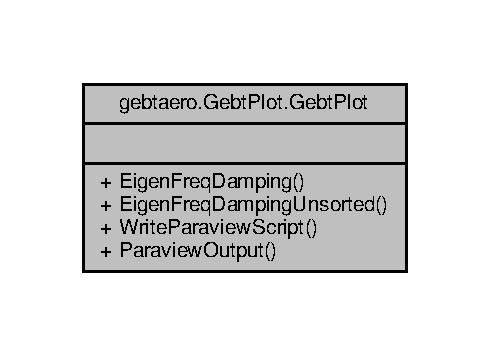
\includegraphics[width=235pt]{classgebtaero_1_1_gebt_plot_1_1_gebt_plot__coll__graph}
\end{center}
\end{figure}
\subsection*{Public Member Functions}
\begin{DoxyCompactItemize}
\item 
def \hyperlink{classgebtaero_1_1_gebt_plot_1_1_gebt_plot_a487ebf0a378a8417070b0e69f73e1970}{Eigen\+Freq\+Damping} (Velocity, Modes, Style=None, Reduced\+Damping=True, Damp\+Axis=False, Damp\+Scale=0.\+01, French=False)
\begin{DoxyCompactList}\small\item\em Generate a matplotlib graph describing some aeroelastic modes. \end{DoxyCompactList}\item 
def \hyperlink{classgebtaero_1_1_gebt_plot_1_1_gebt_plot_ada6addc1b62b7ee88fa482a6a2c7abd1}{Eigen\+Freq\+Damping\+Unsorted} (Velocity, Modes, Style=None, Damp\+Axis=False, Damp\+Scale=0.\+01, French=False)
\begin{DoxyCompactList}\small\item\em a method similar to \hyperlink{classgebtaero_1_1_gebt_plot_1_1_gebt_plot_a487ebf0a378a8417070b0e69f73e1970}{Gebt\+Plot\+::\+Eigen\+Freq\+Damping} for unsorted modes (style point to avoid shift in the curves) \end{DoxyCompactList}\item 
def \hyperlink{classgebtaero_1_1_gebt_plot_1_1_gebt_plot_aada9da700e97eef6c59a4377098954af}{Write\+Paraview\+Script} (Vtk\+Folder, Vtk\+Name, Airfoil\+Path=\char`\"{}/opt/gebtaero/airfoil/airfoil\+\_\+default.\+vtk\char`\"{})
\begin{DoxyCompactList}\small\item\em Write a python paraview script using a folder of vtk output files. \end{DoxyCompactList}\item 
def \hyperlink{classgebtaero_1_1_gebt_plot_1_1_gebt_plot_ae78de8134989ce474d9a7d32b6f7e7c9}{Paraview\+Output} (self, Vtk\+Folder, Vtk\+Name, Airfoil\+Path=\char`\"{}/opt/gebtaero/airfoil/airfoil\+\_\+default.\+vtk\char`\"{})
\begin{DoxyCompactList}\small\item\em Create a paraview script using \hyperlink{classgebtaero_1_1_gebt_plot_1_1_gebt_plot_aada9da700e97eef6c59a4377098954af}{Gebt\+Plot\+::\+Write\+Paraview\+Script} and launch it. \end{DoxyCompactList}\end{DoxyCompactItemize}


\subsection{Detailed Description}
This class is used to generate output using matplotlib and paraview. 

Definition at line 8 of file Gebt\+Plot.\+py.



\subsection{Member Function Documentation}
\mbox{\Hypertarget{classgebtaero_1_1_gebt_plot_1_1_gebt_plot_a487ebf0a378a8417070b0e69f73e1970}\label{classgebtaero_1_1_gebt_plot_1_1_gebt_plot_a487ebf0a378a8417070b0e69f73e1970}} 
\index{gebtaero\+::\+Gebt\+Plot\+::\+Gebt\+Plot@{gebtaero\+::\+Gebt\+Plot\+::\+Gebt\+Plot}!Eigen\+Freq\+Damping@{Eigen\+Freq\+Damping}}
\index{Eigen\+Freq\+Damping@{Eigen\+Freq\+Damping}!gebtaero\+::\+Gebt\+Plot\+::\+Gebt\+Plot@{gebtaero\+::\+Gebt\+Plot\+::\+Gebt\+Plot}}
\subsubsection{\texorpdfstring{Eigen\+Freq\+Damping()}{EigenFreqDamping()}}
{\footnotesize\ttfamily def gebtaero.\+Gebt\+Plot.\+Gebt\+Plot.\+Eigen\+Freq\+Damping (\begin{DoxyParamCaption}\item[{}]{Velocity,  }\item[{}]{Modes,  }\item[{}]{Style = {\ttfamily None},  }\item[{}]{Reduced\+Damping = {\ttfamily True},  }\item[{}]{Damp\+Axis = {\ttfamily False},  }\item[{}]{Damp\+Scale = {\ttfamily 0.01},  }\item[{}]{French = {\ttfamily False} }\end{DoxyParamCaption})}



Generate a matplotlib graph describing some aeroelastic modes. 


\begin{DoxyParams}{Parameters}
{\em Velocity} & a list containing the velocity where the modes are plotted (x axis) \\
\hline
{\em Modes} & a list containing the frequency and the real part of the modes (y axis) \\
\hline
{\em Style} & the style of the curve (matplotlib doc) \\
\hline
{\em Reduced\+Damping} & if true, replace the real part of the mode with the reduced damping (divided by -\/1/(4$\ast$pi$\ast$f)) \\
\hline
{\em Damp\+Axis} & if true,impose the scale of the damping graph \\
\hline
{\em Damp\+Scale} & the scale of the damping graph \\
\hline
\end{DoxyParams}


Definition at line 16 of file Gebt\+Plot.\+py.

\mbox{\Hypertarget{classgebtaero_1_1_gebt_plot_1_1_gebt_plot_ada6addc1b62b7ee88fa482a6a2c7abd1}\label{classgebtaero_1_1_gebt_plot_1_1_gebt_plot_ada6addc1b62b7ee88fa482a6a2c7abd1}} 
\index{gebtaero\+::\+Gebt\+Plot\+::\+Gebt\+Plot@{gebtaero\+::\+Gebt\+Plot\+::\+Gebt\+Plot}!Eigen\+Freq\+Damping\+Unsorted@{Eigen\+Freq\+Damping\+Unsorted}}
\index{Eigen\+Freq\+Damping\+Unsorted@{Eigen\+Freq\+Damping\+Unsorted}!gebtaero\+::\+Gebt\+Plot\+::\+Gebt\+Plot@{gebtaero\+::\+Gebt\+Plot\+::\+Gebt\+Plot}}
\subsubsection{\texorpdfstring{Eigen\+Freq\+Damping\+Unsorted()}{EigenFreqDampingUnsorted()}}
{\footnotesize\ttfamily def gebtaero.\+Gebt\+Plot.\+Gebt\+Plot.\+Eigen\+Freq\+Damping\+Unsorted (\begin{DoxyParamCaption}\item[{}]{Velocity,  }\item[{}]{Modes,  }\item[{}]{Style = {\ttfamily None},  }\item[{}]{Damp\+Axis = {\ttfamily False},  }\item[{}]{Damp\+Scale = {\ttfamily 0.01},  }\item[{}]{French = {\ttfamily False} }\end{DoxyParamCaption})}



a method similar to \hyperlink{classgebtaero_1_1_gebt_plot_1_1_gebt_plot_a487ebf0a378a8417070b0e69f73e1970}{Gebt\+Plot\+::\+Eigen\+Freq\+Damping} for unsorted modes (style point to avoid shift in the curves) 


\begin{DoxyParams}{Parameters}
{\em Velocity} & a list containing the velocity where the modes are plotted (x axis) \\
\hline
{\em Modes} & a list containing the frequency and the real part of the modes (y axis) \\
\hline
{\em Style} & the style of the curve (matplotlib doc) \\
\hline
{\em Damp\+Axis} & if true,impose the scale of the damping graph \\
\hline
{\em Damp\+Scale} & the scale of the damping graph \begin{DoxyVerb}Plot frequencies and Damping of a set of computed modes
\end{DoxyVerb}
 \\
\hline
\end{DoxyParams}


Definition at line 78 of file Gebt\+Plot.\+py.

\mbox{\Hypertarget{classgebtaero_1_1_gebt_plot_1_1_gebt_plot_ae78de8134989ce474d9a7d32b6f7e7c9}\label{classgebtaero_1_1_gebt_plot_1_1_gebt_plot_ae78de8134989ce474d9a7d32b6f7e7c9}} 
\index{gebtaero\+::\+Gebt\+Plot\+::\+Gebt\+Plot@{gebtaero\+::\+Gebt\+Plot\+::\+Gebt\+Plot}!Paraview\+Output@{Paraview\+Output}}
\index{Paraview\+Output@{Paraview\+Output}!gebtaero\+::\+Gebt\+Plot\+::\+Gebt\+Plot@{gebtaero\+::\+Gebt\+Plot\+::\+Gebt\+Plot}}
\subsubsection{\texorpdfstring{Paraview\+Output()}{ParaviewOutput()}}
{\footnotesize\ttfamily def gebtaero.\+Gebt\+Plot.\+Gebt\+Plot.\+Paraview\+Output (\begin{DoxyParamCaption}\item[{}]{self,  }\item[{}]{Vtk\+Folder,  }\item[{}]{Vtk\+Name,  }\item[{}]{Airfoil\+Path = {\ttfamily \char`\"{}/opt/gebtaero/airfoil/airfoil\+\_\+default.vtk\char`\"{}} }\end{DoxyParamCaption})}



Create a paraview script using \hyperlink{classgebtaero_1_1_gebt_plot_1_1_gebt_plot_aada9da700e97eef6c59a4377098954af}{Gebt\+Plot\+::\+Write\+Paraview\+Script} and launch it. 


\begin{DoxyParams}{Parameters}
{\em Vtk\+Folder} & The path of the vtk folder \\
\hline
{\em Vtk\+Name} & the name of the simulation used to determine the name of the vtk files \\
\hline
{\em Airfoil\+Path} & The path of a vtk file describing a 2D airfoil \\
\hline
\end{DoxyParams}


Definition at line 154 of file Gebt\+Plot.\+py.

\mbox{\Hypertarget{classgebtaero_1_1_gebt_plot_1_1_gebt_plot_aada9da700e97eef6c59a4377098954af}\label{classgebtaero_1_1_gebt_plot_1_1_gebt_plot_aada9da700e97eef6c59a4377098954af}} 
\index{gebtaero\+::\+Gebt\+Plot\+::\+Gebt\+Plot@{gebtaero\+::\+Gebt\+Plot\+::\+Gebt\+Plot}!Write\+Paraview\+Script@{Write\+Paraview\+Script}}
\index{Write\+Paraview\+Script@{Write\+Paraview\+Script}!gebtaero\+::\+Gebt\+Plot\+::\+Gebt\+Plot@{gebtaero\+::\+Gebt\+Plot\+::\+Gebt\+Plot}}
\subsubsection{\texorpdfstring{Write\+Paraview\+Script()}{WriteParaviewScript()}}
{\footnotesize\ttfamily def gebtaero.\+Gebt\+Plot.\+Gebt\+Plot.\+Write\+Paraview\+Script (\begin{DoxyParamCaption}\item[{}]{Vtk\+Folder,  }\item[{}]{Vtk\+Name,  }\item[{}]{Airfoil\+Path = {\ttfamily \char`\"{}/opt/gebtaero/airfoil/airfoil\+\_\+default.vtk\char`\"{}} }\end{DoxyParamCaption})}



Write a python paraview script using a folder of vtk output files. 


\begin{DoxyParams}{Parameters}
{\em Vtk\+Folder} & The path of the vtk folder \\
\hline
{\em Vtk\+Name} & the name of the simulation used to determine the name of the vtk files \\
\hline
{\em Airfoil\+Path} & The path of a vtk file describing a 2D airfoil \\
\hline
\end{DoxyParams}


Definition at line 119 of file Gebt\+Plot.\+py.

Here is the caller graph for this function\+:\nopagebreak
\begin{figure}[H]
\begin{center}
\leavevmode
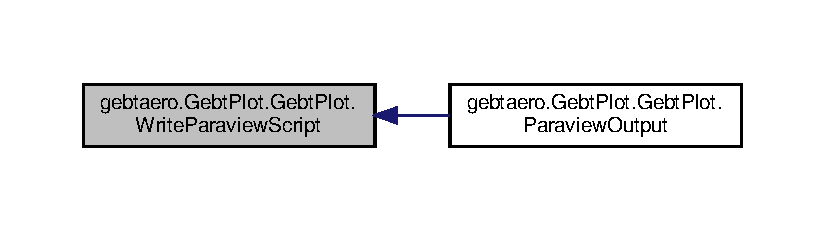
\includegraphics[width=350pt]{classgebtaero_1_1_gebt_plot_1_1_gebt_plot_aada9da700e97eef6c59a4377098954af_icgraph}
\end{center}
\end{figure}


The documentation for this class was generated from the following file\+:\begin{DoxyCompactItemize}
\item 
/home/bertrand/logiciels/gebtaero\+\_\+frama/src/gebtaero/\hyperlink{_gebt_plot_8py}{Gebt\+Plot.\+py}\end{DoxyCompactItemize}

\hypertarget{classgebtaero_1_1_input_file_1_1_input_file}{}\section{gebtaero.\+Input\+File.\+Input\+File Class Reference}
\label{classgebtaero_1_1_input_file_1_1_input_file}\index{gebtaero.\+Input\+File.\+Input\+File@{gebtaero.\+Input\+File.\+Input\+File}}


This class is designed to write the input file .dat readable by the fortran computation code.  


\subsection*{Public Member Functions}
\begin{DoxyCompactItemize}
\item 
def \hyperlink{classgebtaero_1_1_input_file_1_1_input_file_ab2b0171273e5341d432bc98b59208afd}{\+\_\+\+\_\+init\+\_\+\+\_\+} (self, \hyperlink{classgebtaero_1_1_input_file_1_1_input_file_a87afcf626898dba8987e1cee7c4b4ed2}{Name}, \hyperlink{classgebtaero_1_1_input_file_1_1_input_file_a5e345411ff4b135151d46eaa96fd5b82}{Analysis\+Flag}, \hyperlink{classgebtaero_1_1_input_file_1_1_input_file_ad55254b6742bec2601372089bb1f96c4}{Aero\+Flag}, \hyperlink{classgebtaero_1_1_input_file_1_1_input_file_af8b6db9b44fda4dcd69858c0ae6675d2}{Grav\+Flag}, \hyperlink{classgebtaero_1_1_input_file_1_1_input_file_af663735f2e6dc4753c51e27ca4a7cbc6}{Niter}, \hyperlink{classgebtaero_1_1_input_file_1_1_input_file_af000cbafcaa45e8e55ad7e283f3fc10e}{Nstep}, \hyperlink{classgebtaero_1_1_input_file_1_1_input_file_a4cc370b4a5e05b66152449711685c0b8}{Nvtk}, \hyperlink{classgebtaero_1_1_input_file_1_1_input_file_ae7076931e907978fa63e151f549cc8ae}{Nev}, \hyperlink{classgebtaero_1_1_input_file_1_1_input_file_a17d270c516291f04138f9949ae9e6dd3}{A\+C\+Omegaa}, \hyperlink{classgebtaero_1_1_input_file_1_1_input_file_a6163d16b5322a7047dbe227ba5d390e0}{A\+C\+Omegaa\+T\+F\+Number}, \hyperlink{classgebtaero_1_1_input_file_1_1_input_file_af6abd7fc89c0f484e41fe96fc94e72ec}{A\+C\+Va}, \hyperlink{classgebtaero_1_1_input_file_1_1_input_file_adae1dff6c382e115473ad2b915854978}{A\+C\+Va\+T\+F\+Number}, \hyperlink{classgebtaero_1_1_wing_1_1_wing}{Wing}, \hyperlink{classgebtaero_1_1_input_file_1_1_input_file_aa219468b0f01af23063dbf55c5d40e1b}{Vinf}, \hyperlink{classgebtaero_1_1_input_file_1_1_input_file_a71105300fe8cf88253e38529768b998e}{Rho}, \hyperlink{classgebtaero_1_1_input_file_1_1_input_file_a1bf2ed2352dca0749990cccb737fef5a}{Alpha\+AC}, \hyperlink{classgebtaero_1_1_input_file_1_1_input_file_a20868cef3eeb8d6c140d62d2d2252657}{Beta\+AC}, \hyperlink{classgebtaero_1_1_input_file_1_1_input_file_a76efb85d94155e3065ed0139ee3adc5f}{Simu\+Start}, \hyperlink{classgebtaero_1_1_input_file_1_1_input_file_a94164f915c41a24c95ad025f34b7cbcc}{Simu\+End}, \hyperlink{classgebtaero_1_1_input_file_1_1_input_file_a3e49397db5d15285d57c3df5311bf2f8}{Xcg}=0.)
\item 
def \hyperlink{classgebtaero_1_1_input_file_1_1_input_file_acae95b1a0b2631341592cf0abe4178c8}{Get\+Name} (self)
\item 
def \hyperlink{classgebtaero_1_1_input_file_1_1_input_file_a3fe8f05410f29d9c555adbee5dae9e16}{Get\+File\+Name} (self)
\item 
def \hyperlink{classgebtaero_1_1_input_file_1_1_input_file_a8d9a4bed8ff821455af85d5440329fe8}{Get\+Analysis\+Flag} (self)
\item 
def \hyperlink{classgebtaero_1_1_input_file_1_1_input_file_a3cf4d7178dc0471896e7c60f6c17e906}{Append\+Time\+Function} (self, \hyperlink{classgebtaero_1_1_time_function_1_1_time_function}{Time\+Function})
\begin{DoxyCompactList}\small\item\em Add a \hyperlink{namespacegebtaero_1_1_time_function}{Time\+Function} to the \hyperlink{classgebtaero_1_1_input_file_1_1_input_file}{Input\+File}. \end{DoxyCompactList}\item 
def \hyperlink{classgebtaero_1_1_input_file_1_1_input_file_a5d53bb9ae864d002dfbbee1231b91881}{Get\+Time\+Function} (self, index)
\item 
def \hyperlink{classgebtaero_1_1_input_file_1_1_input_file_aff90830e65ba0e25b330c595a94a7a82}{Write\+Input\+File} (self)
\begin{DoxyCompactList}\small\item\em Write a .dat input file readable by the fortran computation code. \end{DoxyCompactList}\item 
def \hyperlink{classgebtaero_1_1_input_file_1_1_input_file_a5c0e5660a7e8a816f2fe3b712480306a}{Remove\+Input\+File} (self)
\begin{DoxyCompactList}\small\item\em Remove the .dat input file, the .ini (initial condition for dynamic simulation) and the input.\+ech (summary of the input process) \end{DoxyCompactList}\item 
def \hyperlink{classgebtaero_1_1_input_file_1_1_input_file_a0138cdf368f06be59a355955c737a3c3}{Write\+Init\+File} (self)
\begin{DoxyCompactList}\small\item\em Write the .ini filled with 0.\+0 for a transient dynamic simulation with no initial displacement or velocity. \end{DoxyCompactList}\end{DoxyCompactItemize}
\subsection*{Public Attributes}
\begin{DoxyCompactItemize}
\item 
\hyperlink{classgebtaero_1_1_input_file_1_1_input_file_a87afcf626898dba8987e1cee7c4b4ed2}{Name}
\begin{DoxyCompactList}\small\item\em the Name of the simulation \end{DoxyCompactList}\item 
\hyperlink{classgebtaero_1_1_input_file_1_1_input_file_a3bb9731a3c44faaf460cb16078183f92}{File\+Name}
\begin{DoxyCompactList}\small\item\em the name on the input file .dat \end{DoxyCompactList}\item 
\hyperlink{classgebtaero_1_1_input_file_1_1_input_file_a5e345411ff4b135151d46eaa96fd5b82}{Analysis\+Flag}
\begin{DoxyCompactList}\small\item\em link to \hyperlink{namespaceioaero_a435527b09d62e7aac9883e1a6d6f3438}{ioaero\+::analysis\+\_\+flag} \end{DoxyCompactList}\item 
\hyperlink{classgebtaero_1_1_input_file_1_1_input_file_ad55254b6742bec2601372089bb1f96c4}{Aero\+Flag}
\begin{DoxyCompactList}\small\item\em link to \hyperlink{namespaceioaero_afb280b6ca8de323c9a07076df81a71e1}{ioaero\+::aero\+\_\+flag} \end{DoxyCompactList}\item 
\hyperlink{classgebtaero_1_1_input_file_1_1_input_file_af8b6db9b44fda4dcd69858c0ae6675d2}{Grav\+Flag}
\begin{DoxyCompactList}\small\item\em link to \hyperlink{namespaceioaero_a831fe87d45ef05e3e29a8c4c2fc88c8f}{ioaero\+::grav\+\_\+flag} \end{DoxyCompactList}\item 
\hyperlink{classgebtaero_1_1_input_file_1_1_input_file_af663735f2e6dc4753c51e27ca4a7cbc6}{Niter}
\begin{DoxyCompactList}\small\item\em link to \hyperlink{namespaceioaero_ac008486fd12e0029a1ef77b3ca5e12c3}{ioaero\+::niter} \end{DoxyCompactList}\item 
\hyperlink{classgebtaero_1_1_input_file_1_1_input_file_af000cbafcaa45e8e55ad7e283f3fc10e}{Nstep}
\begin{DoxyCompactList}\small\item\em link to \hyperlink{namespaceioaero_ab078a397454a22b07a19ae3a7443a561}{ioaero\+::nstep} \end{DoxyCompactList}\item 
\hyperlink{classgebtaero_1_1_input_file_1_1_input_file_a4cc370b4a5e05b66152449711685c0b8}{Nvtk}
\begin{DoxyCompactList}\small\item\em link to \hyperlink{namespaceioaero_a29c506d8ad3a3609366b35e7e4c00fa4}{ioaero\+::nvtk} \end{DoxyCompactList}\item 
\hyperlink{classgebtaero_1_1_input_file_1_1_input_file_ae7076931e907978fa63e151f549cc8ae}{Nev}
\begin{DoxyCompactList}\small\item\em link to \hyperlink{namespaceioaero_a1216c8699aea9eb27e3d795cc9d8d271}{ioaero\+::nev} \end{DoxyCompactList}\item 
\hyperlink{classgebtaero_1_1_input_file_1_1_input_file_a17d270c516291f04138f9949ae9e6dd3}{A\+C\+Omegaa}
\begin{DoxyCompactList}\small\item\em link to \hyperlink{namespaceioaero_a38fc5ef87ae7c2e312ad32f857e791cb}{ioaero\+::omega\+\_\+a0} \end{DoxyCompactList}\item 
\hyperlink{classgebtaero_1_1_input_file_1_1_input_file_a6163d16b5322a7047dbe227ba5d390e0}{A\+C\+Omegaa\+T\+F\+Number}
\begin{DoxyCompactList}\small\item\em link to \hyperlink{namespaceioaero_a9ec25357ecfc1c09628efa147300aaee}{ioaero\+::omega\+\_\+a\+\_\+tf} \end{DoxyCompactList}\item 
\hyperlink{classgebtaero_1_1_input_file_1_1_input_file_af6abd7fc89c0f484e41fe96fc94e72ec}{A\+C\+Va}
\begin{DoxyCompactList}\small\item\em link to \hyperlink{namespaceioaero_a3cefdbd9d62bffe41f44b7f79f321f67}{ioaero\+::v\+\_\+root\+\_\+a0} \end{DoxyCompactList}\item 
\hyperlink{classgebtaero_1_1_input_file_1_1_input_file_adae1dff6c382e115473ad2b915854978}{A\+C\+Va\+T\+F\+Number}
\begin{DoxyCompactList}\small\item\em link to \hyperlink{namespaceioaero_adb4e11942a388b1bf1f13d10c79614bc}{ioaero\+::v\+\_\+root\+\_\+a\+\_\+tf} \end{DoxyCompactList}\item 
\hyperlink{classgebtaero_1_1_input_file_1_1_input_file_aef106e7014301b5094f9ebd82637f282}{Wing}
\begin{DoxyCompactList}\small\item\em the \hyperlink{namespacegebtaero_1_1_wing}{Wing} used in the simulation \end{DoxyCompactList}\item 
\hyperlink{classgebtaero_1_1_input_file_1_1_input_file_aa219468b0f01af23063dbf55c5d40e1b}{Vinf}
\begin{DoxyCompactList}\small\item\em Upstream velocity of the simulation. \end{DoxyCompactList}\item 
\hyperlink{classgebtaero_1_1_input_file_1_1_input_file_a71105300fe8cf88253e38529768b998e}{Rho}
\begin{DoxyCompactList}\small\item\em air density of the simulation \end{DoxyCompactList}\item 
\hyperlink{classgebtaero_1_1_input_file_1_1_input_file_a1bf2ed2352dca0749990cccb737fef5a}{Alpha\+AC}
\begin{DoxyCompactList}\small\item\em Aircraft angle of attack. \end{DoxyCompactList}\item 
\hyperlink{classgebtaero_1_1_input_file_1_1_input_file_a20868cef3eeb8d6c140d62d2d2252657}{Beta\+AC}
\begin{DoxyCompactList}\small\item\em Aircraft yaw angle. \end{DoxyCompactList}\item 
\hyperlink{classgebtaero_1_1_input_file_1_1_input_file_a76efb85d94155e3065ed0139ee3adc5f}{Simu\+Start}
\begin{DoxyCompactList}\small\item\em Start time of the simulation. \end{DoxyCompactList}\item 
\hyperlink{classgebtaero_1_1_input_file_1_1_input_file_a94164f915c41a24c95ad025f34b7cbcc}{Simu\+End}
\begin{DoxyCompactList}\small\item\em End time of the simulation. \end{DoxyCompactList}\item 
\hyperlink{classgebtaero_1_1_input_file_1_1_input_file_a3e49397db5d15285d57c3df5311bf2f8}{Xcg}
\begin{DoxyCompactList}\small\item\em position of center of gravity in frame a \end{DoxyCompactList}\item 
\hyperlink{classgebtaero_1_1_input_file_1_1_input_file_a8e5da9f59ecc39d20885bf47fca12382}{Time\+Functions}
\end{DoxyCompactItemize}


\subsection{Detailed Description}
This class is designed to write the input file .dat readable by the fortran computation code. 

Definition at line 5 of file Input\+File.\+py.



\subsection{Constructor \& Destructor Documentation}
\mbox{\Hypertarget{classgebtaero_1_1_input_file_1_1_input_file_ab2b0171273e5341d432bc98b59208afd}\label{classgebtaero_1_1_input_file_1_1_input_file_ab2b0171273e5341d432bc98b59208afd}} 
\index{gebtaero\+::\+Input\+File\+::\+Input\+File@{gebtaero\+::\+Input\+File\+::\+Input\+File}!\+\_\+\+\_\+init\+\_\+\+\_\+@{\+\_\+\+\_\+init\+\_\+\+\_\+}}
\index{\+\_\+\+\_\+init\+\_\+\+\_\+@{\+\_\+\+\_\+init\+\_\+\+\_\+}!gebtaero\+::\+Input\+File\+::\+Input\+File@{gebtaero\+::\+Input\+File\+::\+Input\+File}}
\subsubsection{\texorpdfstring{\+\_\+\+\_\+init\+\_\+\+\_\+()}{\_\_init\_\_()}}
{\footnotesize\ttfamily def gebtaero.\+Input\+File.\+Input\+File.\+\_\+\+\_\+init\+\_\+\+\_\+ (\begin{DoxyParamCaption}\item[{}]{self,  }\item[{}]{Name,  }\item[{}]{Analysis\+Flag,  }\item[{}]{Aero\+Flag,  }\item[{}]{Grav\+Flag,  }\item[{}]{Niter,  }\item[{}]{Nstep,  }\item[{}]{Nvtk,  }\item[{}]{Nev,  }\item[{}]{A\+C\+Omegaa,  }\item[{}]{A\+C\+Omegaa\+T\+F\+Number,  }\item[{}]{A\+C\+Va,  }\item[{}]{A\+C\+Va\+T\+F\+Number,  }\item[{}]{Wing,  }\item[{}]{Vinf,  }\item[{}]{Rho,  }\item[{}]{Alpha\+AC,  }\item[{}]{Beta\+AC,  }\item[{}]{Simu\+Start,  }\item[{}]{Simu\+End,  }\item[{}]{Xcg = {\ttfamily 0.} }\end{DoxyParamCaption})}



Definition at line 6 of file Input\+File.\+py.



\subsection{Member Function Documentation}
\mbox{\Hypertarget{classgebtaero_1_1_input_file_1_1_input_file_a3cf4d7178dc0471896e7c60f6c17e906}\label{classgebtaero_1_1_input_file_1_1_input_file_a3cf4d7178dc0471896e7c60f6c17e906}} 
\index{gebtaero\+::\+Input\+File\+::\+Input\+File@{gebtaero\+::\+Input\+File\+::\+Input\+File}!Append\+Time\+Function@{Append\+Time\+Function}}
\index{Append\+Time\+Function@{Append\+Time\+Function}!gebtaero\+::\+Input\+File\+::\+Input\+File@{gebtaero\+::\+Input\+File\+::\+Input\+File}}
\subsubsection{\texorpdfstring{Append\+Time\+Function()}{AppendTimeFunction()}}
{\footnotesize\ttfamily def gebtaero.\+Input\+File.\+Input\+File.\+Append\+Time\+Function (\begin{DoxyParamCaption}\item[{}]{self,  }\item[{}]{Time\+Function }\end{DoxyParamCaption})}



Add a \hyperlink{namespacegebtaero_1_1_time_function}{Time\+Function} to the \hyperlink{classgebtaero_1_1_input_file_1_1_input_file}{Input\+File}. 



Definition at line 63 of file Input\+File.\+py.

\mbox{\Hypertarget{classgebtaero_1_1_input_file_1_1_input_file_a8d9a4bed8ff821455af85d5440329fe8}\label{classgebtaero_1_1_input_file_1_1_input_file_a8d9a4bed8ff821455af85d5440329fe8}} 
\index{gebtaero\+::\+Input\+File\+::\+Input\+File@{gebtaero\+::\+Input\+File\+::\+Input\+File}!Get\+Analysis\+Flag@{Get\+Analysis\+Flag}}
\index{Get\+Analysis\+Flag@{Get\+Analysis\+Flag}!gebtaero\+::\+Input\+File\+::\+Input\+File@{gebtaero\+::\+Input\+File\+::\+Input\+File}}
\subsubsection{\texorpdfstring{Get\+Analysis\+Flag()}{GetAnalysisFlag()}}
{\footnotesize\ttfamily def gebtaero.\+Input\+File.\+Input\+File.\+Get\+Analysis\+Flag (\begin{DoxyParamCaption}\item[{}]{self }\end{DoxyParamCaption})}



Definition at line 59 of file Input\+File.\+py.

\mbox{\Hypertarget{classgebtaero_1_1_input_file_1_1_input_file_a3fe8f05410f29d9c555adbee5dae9e16}\label{classgebtaero_1_1_input_file_1_1_input_file_a3fe8f05410f29d9c555adbee5dae9e16}} 
\index{gebtaero\+::\+Input\+File\+::\+Input\+File@{gebtaero\+::\+Input\+File\+::\+Input\+File}!Get\+File\+Name@{Get\+File\+Name}}
\index{Get\+File\+Name@{Get\+File\+Name}!gebtaero\+::\+Input\+File\+::\+Input\+File@{gebtaero\+::\+Input\+File\+::\+Input\+File}}
\subsubsection{\texorpdfstring{Get\+File\+Name()}{GetFileName()}}
{\footnotesize\ttfamily def gebtaero.\+Input\+File.\+Input\+File.\+Get\+File\+Name (\begin{DoxyParamCaption}\item[{}]{self }\end{DoxyParamCaption})}



Definition at line 56 of file Input\+File.\+py.

\mbox{\Hypertarget{classgebtaero_1_1_input_file_1_1_input_file_acae95b1a0b2631341592cf0abe4178c8}\label{classgebtaero_1_1_input_file_1_1_input_file_acae95b1a0b2631341592cf0abe4178c8}} 
\index{gebtaero\+::\+Input\+File\+::\+Input\+File@{gebtaero\+::\+Input\+File\+::\+Input\+File}!Get\+Name@{Get\+Name}}
\index{Get\+Name@{Get\+Name}!gebtaero\+::\+Input\+File\+::\+Input\+File@{gebtaero\+::\+Input\+File\+::\+Input\+File}}
\subsubsection{\texorpdfstring{Get\+Name()}{GetName()}}
{\footnotesize\ttfamily def gebtaero.\+Input\+File.\+Input\+File.\+Get\+Name (\begin{DoxyParamCaption}\item[{}]{self }\end{DoxyParamCaption})}



Definition at line 53 of file Input\+File.\+py.

\mbox{\Hypertarget{classgebtaero_1_1_input_file_1_1_input_file_a5d53bb9ae864d002dfbbee1231b91881}\label{classgebtaero_1_1_input_file_1_1_input_file_a5d53bb9ae864d002dfbbee1231b91881}} 
\index{gebtaero\+::\+Input\+File\+::\+Input\+File@{gebtaero\+::\+Input\+File\+::\+Input\+File}!Get\+Time\+Function@{Get\+Time\+Function}}
\index{Get\+Time\+Function@{Get\+Time\+Function}!gebtaero\+::\+Input\+File\+::\+Input\+File@{gebtaero\+::\+Input\+File\+::\+Input\+File}}
\subsubsection{\texorpdfstring{Get\+Time\+Function()}{GetTimeFunction()}}
{\footnotesize\ttfamily def gebtaero.\+Input\+File.\+Input\+File.\+Get\+Time\+Function (\begin{DoxyParamCaption}\item[{}]{self,  }\item[{}]{index }\end{DoxyParamCaption})}



Definition at line 66 of file Input\+File.\+py.

\mbox{\Hypertarget{classgebtaero_1_1_input_file_1_1_input_file_a5c0e5660a7e8a816f2fe3b712480306a}\label{classgebtaero_1_1_input_file_1_1_input_file_a5c0e5660a7e8a816f2fe3b712480306a}} 
\index{gebtaero\+::\+Input\+File\+::\+Input\+File@{gebtaero\+::\+Input\+File\+::\+Input\+File}!Remove\+Input\+File@{Remove\+Input\+File}}
\index{Remove\+Input\+File@{Remove\+Input\+File}!gebtaero\+::\+Input\+File\+::\+Input\+File@{gebtaero\+::\+Input\+File\+::\+Input\+File}}
\subsubsection{\texorpdfstring{Remove\+Input\+File()}{RemoveInputFile()}}
{\footnotesize\ttfamily def gebtaero.\+Input\+File.\+Input\+File.\+Remove\+Input\+File (\begin{DoxyParamCaption}\item[{}]{self }\end{DoxyParamCaption})}



Remove the .dat input file, the .ini (initial condition for dynamic simulation) and the input.\+ech (summary of the input process) 



Definition at line 225 of file Input\+File.\+py.

\mbox{\Hypertarget{classgebtaero_1_1_input_file_1_1_input_file_a0138cdf368f06be59a355955c737a3c3}\label{classgebtaero_1_1_input_file_1_1_input_file_a0138cdf368f06be59a355955c737a3c3}} 
\index{gebtaero\+::\+Input\+File\+::\+Input\+File@{gebtaero\+::\+Input\+File\+::\+Input\+File}!Write\+Init\+File@{Write\+Init\+File}}
\index{Write\+Init\+File@{Write\+Init\+File}!gebtaero\+::\+Input\+File\+::\+Input\+File@{gebtaero\+::\+Input\+File\+::\+Input\+File}}
\subsubsection{\texorpdfstring{Write\+Init\+File()}{WriteInitFile()}}
{\footnotesize\ttfamily def gebtaero.\+Input\+File.\+Input\+File.\+Write\+Init\+File (\begin{DoxyParamCaption}\item[{}]{self }\end{DoxyParamCaption})}



Write the .ini filled with 0.\+0 for a transient dynamic simulation with no initial displacement or velocity. 



Definition at line 230 of file Input\+File.\+py.

\mbox{\Hypertarget{classgebtaero_1_1_input_file_1_1_input_file_aff90830e65ba0e25b330c595a94a7a82}\label{classgebtaero_1_1_input_file_1_1_input_file_aff90830e65ba0e25b330c595a94a7a82}} 
\index{gebtaero\+::\+Input\+File\+::\+Input\+File@{gebtaero\+::\+Input\+File\+::\+Input\+File}!Write\+Input\+File@{Write\+Input\+File}}
\index{Write\+Input\+File@{Write\+Input\+File}!gebtaero\+::\+Input\+File\+::\+Input\+File@{gebtaero\+::\+Input\+File\+::\+Input\+File}}
\subsubsection{\texorpdfstring{Write\+Input\+File()}{WriteInputFile()}}
{\footnotesize\ttfamily def gebtaero.\+Input\+File.\+Input\+File.\+Write\+Input\+File (\begin{DoxyParamCaption}\item[{}]{self }\end{DoxyParamCaption})}



Write a .dat input file readable by the fortran computation code. 



Definition at line 70 of file Input\+File.\+py.



\subsection{Member Data Documentation}
\mbox{\Hypertarget{classgebtaero_1_1_input_file_1_1_input_file_a17d270c516291f04138f9949ae9e6dd3}\label{classgebtaero_1_1_input_file_1_1_input_file_a17d270c516291f04138f9949ae9e6dd3}} 
\index{gebtaero\+::\+Input\+File\+::\+Input\+File@{gebtaero\+::\+Input\+File\+::\+Input\+File}!A\+C\+Omegaa@{A\+C\+Omegaa}}
\index{A\+C\+Omegaa@{A\+C\+Omegaa}!gebtaero\+::\+Input\+File\+::\+Input\+File@{gebtaero\+::\+Input\+File\+::\+Input\+File}}
\subsubsection{\texorpdfstring{A\+C\+Omegaa}{ACOmegaa}}
{\footnotesize\ttfamily gebtaero.\+Input\+File.\+Input\+File.\+A\+C\+Omegaa}



link to \hyperlink{namespaceioaero_a38fc5ef87ae7c2e312ad32f857e791cb}{ioaero\+::omega\+\_\+a0} 



Definition at line 26 of file Input\+File.\+py.

\mbox{\Hypertarget{classgebtaero_1_1_input_file_1_1_input_file_a6163d16b5322a7047dbe227ba5d390e0}\label{classgebtaero_1_1_input_file_1_1_input_file_a6163d16b5322a7047dbe227ba5d390e0}} 
\index{gebtaero\+::\+Input\+File\+::\+Input\+File@{gebtaero\+::\+Input\+File\+::\+Input\+File}!A\+C\+Omegaa\+T\+F\+Number@{A\+C\+Omegaa\+T\+F\+Number}}
\index{A\+C\+Omegaa\+T\+F\+Number@{A\+C\+Omegaa\+T\+F\+Number}!gebtaero\+::\+Input\+File\+::\+Input\+File@{gebtaero\+::\+Input\+File\+::\+Input\+File}}
\subsubsection{\texorpdfstring{A\+C\+Omegaa\+T\+F\+Number}{ACOmegaaTFNumber}}
{\footnotesize\ttfamily gebtaero.\+Input\+File.\+Input\+File.\+A\+C\+Omegaa\+T\+F\+Number}



link to \hyperlink{namespaceioaero_a9ec25357ecfc1c09628efa147300aaee}{ioaero\+::omega\+\_\+a\+\_\+tf} 



Definition at line 28 of file Input\+File.\+py.

\mbox{\Hypertarget{classgebtaero_1_1_input_file_1_1_input_file_af6abd7fc89c0f484e41fe96fc94e72ec}\label{classgebtaero_1_1_input_file_1_1_input_file_af6abd7fc89c0f484e41fe96fc94e72ec}} 
\index{gebtaero\+::\+Input\+File\+::\+Input\+File@{gebtaero\+::\+Input\+File\+::\+Input\+File}!A\+C\+Va@{A\+C\+Va}}
\index{A\+C\+Va@{A\+C\+Va}!gebtaero\+::\+Input\+File\+::\+Input\+File@{gebtaero\+::\+Input\+File\+::\+Input\+File}}
\subsubsection{\texorpdfstring{A\+C\+Va}{ACVa}}
{\footnotesize\ttfamily gebtaero.\+Input\+File.\+Input\+File.\+A\+C\+Va}



link to \hyperlink{namespaceioaero_a3cefdbd9d62bffe41f44b7f79f321f67}{ioaero\+::v\+\_\+root\+\_\+a0} 



Definition at line 30 of file Input\+File.\+py.

\mbox{\Hypertarget{classgebtaero_1_1_input_file_1_1_input_file_adae1dff6c382e115473ad2b915854978}\label{classgebtaero_1_1_input_file_1_1_input_file_adae1dff6c382e115473ad2b915854978}} 
\index{gebtaero\+::\+Input\+File\+::\+Input\+File@{gebtaero\+::\+Input\+File\+::\+Input\+File}!A\+C\+Va\+T\+F\+Number@{A\+C\+Va\+T\+F\+Number}}
\index{A\+C\+Va\+T\+F\+Number@{A\+C\+Va\+T\+F\+Number}!gebtaero\+::\+Input\+File\+::\+Input\+File@{gebtaero\+::\+Input\+File\+::\+Input\+File}}
\subsubsection{\texorpdfstring{A\+C\+Va\+T\+F\+Number}{ACVaTFNumber}}
{\footnotesize\ttfamily gebtaero.\+Input\+File.\+Input\+File.\+A\+C\+Va\+T\+F\+Number}



link to \hyperlink{namespaceioaero_adb4e11942a388b1bf1f13d10c79614bc}{ioaero\+::v\+\_\+root\+\_\+a\+\_\+tf} 



Definition at line 32 of file Input\+File.\+py.

\mbox{\Hypertarget{classgebtaero_1_1_input_file_1_1_input_file_ad55254b6742bec2601372089bb1f96c4}\label{classgebtaero_1_1_input_file_1_1_input_file_ad55254b6742bec2601372089bb1f96c4}} 
\index{gebtaero\+::\+Input\+File\+::\+Input\+File@{gebtaero\+::\+Input\+File\+::\+Input\+File}!Aero\+Flag@{Aero\+Flag}}
\index{Aero\+Flag@{Aero\+Flag}!gebtaero\+::\+Input\+File\+::\+Input\+File@{gebtaero\+::\+Input\+File\+::\+Input\+File}}
\subsubsection{\texorpdfstring{Aero\+Flag}{AeroFlag}}
{\footnotesize\ttfamily gebtaero.\+Input\+File.\+Input\+File.\+Aero\+Flag}



link to \hyperlink{namespaceioaero_afb280b6ca8de323c9a07076df81a71e1}{ioaero\+::aero\+\_\+flag} 



Definition at line 14 of file Input\+File.\+py.

\mbox{\Hypertarget{classgebtaero_1_1_input_file_1_1_input_file_a1bf2ed2352dca0749990cccb737fef5a}\label{classgebtaero_1_1_input_file_1_1_input_file_a1bf2ed2352dca0749990cccb737fef5a}} 
\index{gebtaero\+::\+Input\+File\+::\+Input\+File@{gebtaero\+::\+Input\+File\+::\+Input\+File}!Alpha\+AC@{Alpha\+AC}}
\index{Alpha\+AC@{Alpha\+AC}!gebtaero\+::\+Input\+File\+::\+Input\+File@{gebtaero\+::\+Input\+File\+::\+Input\+File}}
\subsubsection{\texorpdfstring{Alpha\+AC}{AlphaAC}}
{\footnotesize\ttfamily gebtaero.\+Input\+File.\+Input\+File.\+Alpha\+AC}



Aircraft angle of attack. 



Definition at line 40 of file Input\+File.\+py.

\mbox{\Hypertarget{classgebtaero_1_1_input_file_1_1_input_file_a5e345411ff4b135151d46eaa96fd5b82}\label{classgebtaero_1_1_input_file_1_1_input_file_a5e345411ff4b135151d46eaa96fd5b82}} 
\index{gebtaero\+::\+Input\+File\+::\+Input\+File@{gebtaero\+::\+Input\+File\+::\+Input\+File}!Analysis\+Flag@{Analysis\+Flag}}
\index{Analysis\+Flag@{Analysis\+Flag}!gebtaero\+::\+Input\+File\+::\+Input\+File@{gebtaero\+::\+Input\+File\+::\+Input\+File}}
\subsubsection{\texorpdfstring{Analysis\+Flag}{AnalysisFlag}}
{\footnotesize\ttfamily gebtaero.\+Input\+File.\+Input\+File.\+Analysis\+Flag}



link to \hyperlink{namespaceioaero_a435527b09d62e7aac9883e1a6d6f3438}{ioaero\+::analysis\+\_\+flag} 



Definition at line 12 of file Input\+File.\+py.

\mbox{\Hypertarget{classgebtaero_1_1_input_file_1_1_input_file_a20868cef3eeb8d6c140d62d2d2252657}\label{classgebtaero_1_1_input_file_1_1_input_file_a20868cef3eeb8d6c140d62d2d2252657}} 
\index{gebtaero\+::\+Input\+File\+::\+Input\+File@{gebtaero\+::\+Input\+File\+::\+Input\+File}!Beta\+AC@{Beta\+AC}}
\index{Beta\+AC@{Beta\+AC}!gebtaero\+::\+Input\+File\+::\+Input\+File@{gebtaero\+::\+Input\+File\+::\+Input\+File}}
\subsubsection{\texorpdfstring{Beta\+AC}{BetaAC}}
{\footnotesize\ttfamily gebtaero.\+Input\+File.\+Input\+File.\+Beta\+AC}



Aircraft yaw angle. 



Definition at line 42 of file Input\+File.\+py.

\mbox{\Hypertarget{classgebtaero_1_1_input_file_1_1_input_file_a3bb9731a3c44faaf460cb16078183f92}\label{classgebtaero_1_1_input_file_1_1_input_file_a3bb9731a3c44faaf460cb16078183f92}} 
\index{gebtaero\+::\+Input\+File\+::\+Input\+File@{gebtaero\+::\+Input\+File\+::\+Input\+File}!File\+Name@{File\+Name}}
\index{File\+Name@{File\+Name}!gebtaero\+::\+Input\+File\+::\+Input\+File@{gebtaero\+::\+Input\+File\+::\+Input\+File}}
\subsubsection{\texorpdfstring{File\+Name}{FileName}}
{\footnotesize\ttfamily gebtaero.\+Input\+File.\+Input\+File.\+File\+Name}



the name on the input file .dat 



Definition at line 10 of file Input\+File.\+py.

\mbox{\Hypertarget{classgebtaero_1_1_input_file_1_1_input_file_af8b6db9b44fda4dcd69858c0ae6675d2}\label{classgebtaero_1_1_input_file_1_1_input_file_af8b6db9b44fda4dcd69858c0ae6675d2}} 
\index{gebtaero\+::\+Input\+File\+::\+Input\+File@{gebtaero\+::\+Input\+File\+::\+Input\+File}!Grav\+Flag@{Grav\+Flag}}
\index{Grav\+Flag@{Grav\+Flag}!gebtaero\+::\+Input\+File\+::\+Input\+File@{gebtaero\+::\+Input\+File\+::\+Input\+File}}
\subsubsection{\texorpdfstring{Grav\+Flag}{GravFlag}}
{\footnotesize\ttfamily gebtaero.\+Input\+File.\+Input\+File.\+Grav\+Flag}



link to \hyperlink{namespaceioaero_a831fe87d45ef05e3e29a8c4c2fc88c8f}{ioaero\+::grav\+\_\+flag} 



Definition at line 16 of file Input\+File.\+py.

\mbox{\Hypertarget{classgebtaero_1_1_input_file_1_1_input_file_a87afcf626898dba8987e1cee7c4b4ed2}\label{classgebtaero_1_1_input_file_1_1_input_file_a87afcf626898dba8987e1cee7c4b4ed2}} 
\index{gebtaero\+::\+Input\+File\+::\+Input\+File@{gebtaero\+::\+Input\+File\+::\+Input\+File}!Name@{Name}}
\index{Name@{Name}!gebtaero\+::\+Input\+File\+::\+Input\+File@{gebtaero\+::\+Input\+File\+::\+Input\+File}}
\subsubsection{\texorpdfstring{Name}{Name}}
{\footnotesize\ttfamily gebtaero.\+Input\+File.\+Input\+File.\+Name}



the Name of the simulation 



Definition at line 8 of file Input\+File.\+py.

\mbox{\Hypertarget{classgebtaero_1_1_input_file_1_1_input_file_ae7076931e907978fa63e151f549cc8ae}\label{classgebtaero_1_1_input_file_1_1_input_file_ae7076931e907978fa63e151f549cc8ae}} 
\index{gebtaero\+::\+Input\+File\+::\+Input\+File@{gebtaero\+::\+Input\+File\+::\+Input\+File}!Nev@{Nev}}
\index{Nev@{Nev}!gebtaero\+::\+Input\+File\+::\+Input\+File@{gebtaero\+::\+Input\+File\+::\+Input\+File}}
\subsubsection{\texorpdfstring{Nev}{Nev}}
{\footnotesize\ttfamily gebtaero.\+Input\+File.\+Input\+File.\+Nev}



link to \hyperlink{namespaceioaero_a1216c8699aea9eb27e3d795cc9d8d271}{ioaero\+::nev} 



Definition at line 24 of file Input\+File.\+py.

\mbox{\Hypertarget{classgebtaero_1_1_input_file_1_1_input_file_af663735f2e6dc4753c51e27ca4a7cbc6}\label{classgebtaero_1_1_input_file_1_1_input_file_af663735f2e6dc4753c51e27ca4a7cbc6}} 
\index{gebtaero\+::\+Input\+File\+::\+Input\+File@{gebtaero\+::\+Input\+File\+::\+Input\+File}!Niter@{Niter}}
\index{Niter@{Niter}!gebtaero\+::\+Input\+File\+::\+Input\+File@{gebtaero\+::\+Input\+File\+::\+Input\+File}}
\subsubsection{\texorpdfstring{Niter}{Niter}}
{\footnotesize\ttfamily gebtaero.\+Input\+File.\+Input\+File.\+Niter}



link to \hyperlink{namespaceioaero_ac008486fd12e0029a1ef77b3ca5e12c3}{ioaero\+::niter} 



Definition at line 18 of file Input\+File.\+py.

\mbox{\Hypertarget{classgebtaero_1_1_input_file_1_1_input_file_af000cbafcaa45e8e55ad7e283f3fc10e}\label{classgebtaero_1_1_input_file_1_1_input_file_af000cbafcaa45e8e55ad7e283f3fc10e}} 
\index{gebtaero\+::\+Input\+File\+::\+Input\+File@{gebtaero\+::\+Input\+File\+::\+Input\+File}!Nstep@{Nstep}}
\index{Nstep@{Nstep}!gebtaero\+::\+Input\+File\+::\+Input\+File@{gebtaero\+::\+Input\+File\+::\+Input\+File}}
\subsubsection{\texorpdfstring{Nstep}{Nstep}}
{\footnotesize\ttfamily gebtaero.\+Input\+File.\+Input\+File.\+Nstep}



link to \hyperlink{namespaceioaero_ab078a397454a22b07a19ae3a7443a561}{ioaero\+::nstep} 



Definition at line 20 of file Input\+File.\+py.

\mbox{\Hypertarget{classgebtaero_1_1_input_file_1_1_input_file_a4cc370b4a5e05b66152449711685c0b8}\label{classgebtaero_1_1_input_file_1_1_input_file_a4cc370b4a5e05b66152449711685c0b8}} 
\index{gebtaero\+::\+Input\+File\+::\+Input\+File@{gebtaero\+::\+Input\+File\+::\+Input\+File}!Nvtk@{Nvtk}}
\index{Nvtk@{Nvtk}!gebtaero\+::\+Input\+File\+::\+Input\+File@{gebtaero\+::\+Input\+File\+::\+Input\+File}}
\subsubsection{\texorpdfstring{Nvtk}{Nvtk}}
{\footnotesize\ttfamily gebtaero.\+Input\+File.\+Input\+File.\+Nvtk}



link to \hyperlink{namespaceioaero_a29c506d8ad3a3609366b35e7e4c00fa4}{ioaero\+::nvtk} 



Definition at line 22 of file Input\+File.\+py.

\mbox{\Hypertarget{classgebtaero_1_1_input_file_1_1_input_file_a71105300fe8cf88253e38529768b998e}\label{classgebtaero_1_1_input_file_1_1_input_file_a71105300fe8cf88253e38529768b998e}} 
\index{gebtaero\+::\+Input\+File\+::\+Input\+File@{gebtaero\+::\+Input\+File\+::\+Input\+File}!Rho@{Rho}}
\index{Rho@{Rho}!gebtaero\+::\+Input\+File\+::\+Input\+File@{gebtaero\+::\+Input\+File\+::\+Input\+File}}
\subsubsection{\texorpdfstring{Rho}{Rho}}
{\footnotesize\ttfamily gebtaero.\+Input\+File.\+Input\+File.\+Rho}



air density of the simulation 



Definition at line 38 of file Input\+File.\+py.

\mbox{\Hypertarget{classgebtaero_1_1_input_file_1_1_input_file_a94164f915c41a24c95ad025f34b7cbcc}\label{classgebtaero_1_1_input_file_1_1_input_file_a94164f915c41a24c95ad025f34b7cbcc}} 
\index{gebtaero\+::\+Input\+File\+::\+Input\+File@{gebtaero\+::\+Input\+File\+::\+Input\+File}!Simu\+End@{Simu\+End}}
\index{Simu\+End@{Simu\+End}!gebtaero\+::\+Input\+File\+::\+Input\+File@{gebtaero\+::\+Input\+File\+::\+Input\+File}}
\subsubsection{\texorpdfstring{Simu\+End}{SimuEnd}}
{\footnotesize\ttfamily gebtaero.\+Input\+File.\+Input\+File.\+Simu\+End}



End time of the simulation. 



Definition at line 46 of file Input\+File.\+py.

\mbox{\Hypertarget{classgebtaero_1_1_input_file_1_1_input_file_a76efb85d94155e3065ed0139ee3adc5f}\label{classgebtaero_1_1_input_file_1_1_input_file_a76efb85d94155e3065ed0139ee3adc5f}} 
\index{gebtaero\+::\+Input\+File\+::\+Input\+File@{gebtaero\+::\+Input\+File\+::\+Input\+File}!Simu\+Start@{Simu\+Start}}
\index{Simu\+Start@{Simu\+Start}!gebtaero\+::\+Input\+File\+::\+Input\+File@{gebtaero\+::\+Input\+File\+::\+Input\+File}}
\subsubsection{\texorpdfstring{Simu\+Start}{SimuStart}}
{\footnotesize\ttfamily gebtaero.\+Input\+File.\+Input\+File.\+Simu\+Start}



Start time of the simulation. 



Definition at line 44 of file Input\+File.\+py.

\mbox{\Hypertarget{classgebtaero_1_1_input_file_1_1_input_file_a8e5da9f59ecc39d20885bf47fca12382}\label{classgebtaero_1_1_input_file_1_1_input_file_a8e5da9f59ecc39d20885bf47fca12382}} 
\index{gebtaero\+::\+Input\+File\+::\+Input\+File@{gebtaero\+::\+Input\+File\+::\+Input\+File}!Time\+Functions@{Time\+Functions}}
\index{Time\+Functions@{Time\+Functions}!gebtaero\+::\+Input\+File\+::\+Input\+File@{gebtaero\+::\+Input\+File\+::\+Input\+File}}
\subsubsection{\texorpdfstring{Time\+Functions}{TimeFunctions}}
{\footnotesize\ttfamily gebtaero.\+Input\+File.\+Input\+File.\+Time\+Functions}



Definition at line 51 of file Input\+File.\+py.

\mbox{\Hypertarget{classgebtaero_1_1_input_file_1_1_input_file_aa219468b0f01af23063dbf55c5d40e1b}\label{classgebtaero_1_1_input_file_1_1_input_file_aa219468b0f01af23063dbf55c5d40e1b}} 
\index{gebtaero\+::\+Input\+File\+::\+Input\+File@{gebtaero\+::\+Input\+File\+::\+Input\+File}!Vinf@{Vinf}}
\index{Vinf@{Vinf}!gebtaero\+::\+Input\+File\+::\+Input\+File@{gebtaero\+::\+Input\+File\+::\+Input\+File}}
\subsubsection{\texorpdfstring{Vinf}{Vinf}}
{\footnotesize\ttfamily gebtaero.\+Input\+File.\+Input\+File.\+Vinf}



Upstream velocity of the simulation. 



Definition at line 36 of file Input\+File.\+py.

\mbox{\Hypertarget{classgebtaero_1_1_input_file_1_1_input_file_aef106e7014301b5094f9ebd82637f282}\label{classgebtaero_1_1_input_file_1_1_input_file_aef106e7014301b5094f9ebd82637f282}} 
\index{gebtaero\+::\+Input\+File\+::\+Input\+File@{gebtaero\+::\+Input\+File\+::\+Input\+File}!Wing@{Wing}}
\index{Wing@{Wing}!gebtaero\+::\+Input\+File\+::\+Input\+File@{gebtaero\+::\+Input\+File\+::\+Input\+File}}
\subsubsection{\texorpdfstring{Wing}{Wing}}
{\footnotesize\ttfamily gebtaero.\+Input\+File.\+Input\+File.\+Wing}



the \hyperlink{namespacegebtaero_1_1_wing}{Wing} used in the simulation 



Definition at line 34 of file Input\+File.\+py.

\mbox{\Hypertarget{classgebtaero_1_1_input_file_1_1_input_file_a3e49397db5d15285d57c3df5311bf2f8}\label{classgebtaero_1_1_input_file_1_1_input_file_a3e49397db5d15285d57c3df5311bf2f8}} 
\index{gebtaero\+::\+Input\+File\+::\+Input\+File@{gebtaero\+::\+Input\+File\+::\+Input\+File}!Xcg@{Xcg}}
\index{Xcg@{Xcg}!gebtaero\+::\+Input\+File\+::\+Input\+File@{gebtaero\+::\+Input\+File\+::\+Input\+File}}
\subsubsection{\texorpdfstring{Xcg}{Xcg}}
{\footnotesize\ttfamily gebtaero.\+Input\+File.\+Input\+File.\+Xcg}



position of center of gravity in frame a 



Definition at line 48 of file Input\+File.\+py.



The documentation for this class was generated from the following file\+:\begin{DoxyCompactItemize}
\item 
/home/bertrand/logiciels/gebtaero\+\_\+frama/src/gebtaero/\hyperlink{_input_file_8py}{Input\+File.\+py}\end{DoxyCompactItemize}

\hypertarget{classgebtaero_1_1_iso_material_1_1_iso_material}{}\section{gebtaero.\+Iso\+Material.\+Iso\+Material Class Reference}
\label{classgebtaero_1_1_iso_material_1_1_iso_material}\index{gebtaero.\+Iso\+Material.\+Iso\+Material@{gebtaero.\+Iso\+Material.\+Iso\+Material}}


This class correspond to the T\+Y\+PE=I\+SO of the $\ast$\+E\+L\+A\+S\+T\+IC input card of ccx solver.  




Collaboration diagram for gebtaero.\+Iso\+Material.\+Iso\+Material\+:\nopagebreak
\begin{figure}[H]
\begin{center}
\leavevmode
\includegraphics[width=202pt]{classgebtaero_1_1_iso_material_1_1_iso_material__coll__graph}
\end{center}
\end{figure}
\subsection*{Public Member Functions}
\begin{DoxyCompactItemize}
\item 
def \hyperlink{classgebtaero_1_1_iso_material_1_1_iso_material_ae9bef5bb23ffa56bd8342ecb0bf11ced}{\+\_\+\+\_\+init\+\_\+\+\_\+} (self, \hyperlink{classgebtaero_1_1_iso_material_1_1_iso_material_a95ef904760eb41f521d8a921fc44e5ba}{E}, \hyperlink{classgebtaero_1_1_iso_material_1_1_iso_material_a1a590e5600152a083c4ee3d0fb12451a}{Nu}, \hyperlink{classgebtaero_1_1_iso_material_1_1_iso_material_ace8e4cdd649efe5f36fd0093afa6b93a}{Rho}=None)
\item 
def \hyperlink{classgebtaero_1_1_iso_material_1_1_iso_material_aa8457a623f8f6f0e390acecea84b7ae4}{Get\+Iso} (self)
\item 
def \hyperlink{classgebtaero_1_1_iso_material_1_1_iso_material_a8efa18b7c42252bca0f1232916545920}{Get\+Density} (self)
\end{DoxyCompactItemize}
\subsection*{Public Attributes}
\begin{DoxyCompactItemize}
\item 
\hyperlink{classgebtaero_1_1_iso_material_1_1_iso_material_a95ef904760eb41f521d8a921fc44e5ba}{E}
\begin{DoxyCompactList}\small\item\em Young Modulus. \end{DoxyCompactList}\item 
\hyperlink{classgebtaero_1_1_iso_material_1_1_iso_material_a1a590e5600152a083c4ee3d0fb12451a}{Nu}
\begin{DoxyCompactList}\small\item\em Poisson Ratio. \end{DoxyCompactList}\item 
\hyperlink{classgebtaero_1_1_iso_material_1_1_iso_material_ace8e4cdd649efe5f36fd0093afa6b93a}{Rho}
\begin{DoxyCompactList}\small\item\em Density. \end{DoxyCompactList}\end{DoxyCompactItemize}


\subsection{Detailed Description}
This class correspond to the T\+Y\+PE=I\+SO of the $\ast$\+E\+L\+A\+S\+T\+IC input card of ccx solver. 

Definition at line 4 of file Iso\+Material.\+py.



\subsection{Constructor \& Destructor Documentation}
\mbox{\Hypertarget{classgebtaero_1_1_iso_material_1_1_iso_material_ae9bef5bb23ffa56bd8342ecb0bf11ced}\label{classgebtaero_1_1_iso_material_1_1_iso_material_ae9bef5bb23ffa56bd8342ecb0bf11ced}} 
\index{gebtaero\+::\+Iso\+Material\+::\+Iso\+Material@{gebtaero\+::\+Iso\+Material\+::\+Iso\+Material}!\+\_\+\+\_\+init\+\_\+\+\_\+@{\+\_\+\+\_\+init\+\_\+\+\_\+}}
\index{\+\_\+\+\_\+init\+\_\+\+\_\+@{\+\_\+\+\_\+init\+\_\+\+\_\+}!gebtaero\+::\+Iso\+Material\+::\+Iso\+Material@{gebtaero\+::\+Iso\+Material\+::\+Iso\+Material}}
\subsubsection{\texorpdfstring{\+\_\+\+\_\+init\+\_\+\+\_\+()}{\_\_init\_\_()}}
{\footnotesize\ttfamily def gebtaero.\+Iso\+Material.\+Iso\+Material.\+\_\+\+\_\+init\+\_\+\+\_\+ (\begin{DoxyParamCaption}\item[{}]{self,  }\item[{}]{E,  }\item[{}]{Nu,  }\item[{}]{Rho = {\ttfamily None} }\end{DoxyParamCaption})}



Definition at line 5 of file Iso\+Material.\+py.



\subsection{Member Function Documentation}
\mbox{\Hypertarget{classgebtaero_1_1_iso_material_1_1_iso_material_a8efa18b7c42252bca0f1232916545920}\label{classgebtaero_1_1_iso_material_1_1_iso_material_a8efa18b7c42252bca0f1232916545920}} 
\index{gebtaero\+::\+Iso\+Material\+::\+Iso\+Material@{gebtaero\+::\+Iso\+Material\+::\+Iso\+Material}!Get\+Density@{Get\+Density}}
\index{Get\+Density@{Get\+Density}!gebtaero\+::\+Iso\+Material\+::\+Iso\+Material@{gebtaero\+::\+Iso\+Material\+::\+Iso\+Material}}
\subsubsection{\texorpdfstring{Get\+Density()}{GetDensity()}}
{\footnotesize\ttfamily def gebtaero.\+Iso\+Material.\+Iso\+Material.\+Get\+Density (\begin{DoxyParamCaption}\item[{}]{self }\end{DoxyParamCaption})}



Definition at line 16 of file Iso\+Material.\+py.

\mbox{\Hypertarget{classgebtaero_1_1_iso_material_1_1_iso_material_aa8457a623f8f6f0e390acecea84b7ae4}\label{classgebtaero_1_1_iso_material_1_1_iso_material_aa8457a623f8f6f0e390acecea84b7ae4}} 
\index{gebtaero\+::\+Iso\+Material\+::\+Iso\+Material@{gebtaero\+::\+Iso\+Material\+::\+Iso\+Material}!Get\+Iso@{Get\+Iso}}
\index{Get\+Iso@{Get\+Iso}!gebtaero\+::\+Iso\+Material\+::\+Iso\+Material@{gebtaero\+::\+Iso\+Material\+::\+Iso\+Material}}
\subsubsection{\texorpdfstring{Get\+Iso()}{GetIso()}}
{\footnotesize\ttfamily def gebtaero.\+Iso\+Material.\+Iso\+Material.\+Get\+Iso (\begin{DoxyParamCaption}\item[{}]{self }\end{DoxyParamCaption})}



Definition at line 13 of file Iso\+Material.\+py.



\subsection{Member Data Documentation}
\mbox{\Hypertarget{classgebtaero_1_1_iso_material_1_1_iso_material_a95ef904760eb41f521d8a921fc44e5ba}\label{classgebtaero_1_1_iso_material_1_1_iso_material_a95ef904760eb41f521d8a921fc44e5ba}} 
\index{gebtaero\+::\+Iso\+Material\+::\+Iso\+Material@{gebtaero\+::\+Iso\+Material\+::\+Iso\+Material}!E@{E}}
\index{E@{E}!gebtaero\+::\+Iso\+Material\+::\+Iso\+Material@{gebtaero\+::\+Iso\+Material\+::\+Iso\+Material}}
\subsubsection{\texorpdfstring{E}{E}}
{\footnotesize\ttfamily gebtaero.\+Iso\+Material.\+Iso\+Material.\+E}



Young Modulus. 



Definition at line 7 of file Iso\+Material.\+py.

\mbox{\Hypertarget{classgebtaero_1_1_iso_material_1_1_iso_material_a1a590e5600152a083c4ee3d0fb12451a}\label{classgebtaero_1_1_iso_material_1_1_iso_material_a1a590e5600152a083c4ee3d0fb12451a}} 
\index{gebtaero\+::\+Iso\+Material\+::\+Iso\+Material@{gebtaero\+::\+Iso\+Material\+::\+Iso\+Material}!Nu@{Nu}}
\index{Nu@{Nu}!gebtaero\+::\+Iso\+Material\+::\+Iso\+Material@{gebtaero\+::\+Iso\+Material\+::\+Iso\+Material}}
\subsubsection{\texorpdfstring{Nu}{Nu}}
{\footnotesize\ttfamily gebtaero.\+Iso\+Material.\+Iso\+Material.\+Nu}



Poisson Ratio. 



Definition at line 9 of file Iso\+Material.\+py.

\mbox{\Hypertarget{classgebtaero_1_1_iso_material_1_1_iso_material_ace8e4cdd649efe5f36fd0093afa6b93a}\label{classgebtaero_1_1_iso_material_1_1_iso_material_ace8e4cdd649efe5f36fd0093afa6b93a}} 
\index{gebtaero\+::\+Iso\+Material\+::\+Iso\+Material@{gebtaero\+::\+Iso\+Material\+::\+Iso\+Material}!Rho@{Rho}}
\index{Rho@{Rho}!gebtaero\+::\+Iso\+Material\+::\+Iso\+Material@{gebtaero\+::\+Iso\+Material\+::\+Iso\+Material}}
\subsubsection{\texorpdfstring{Rho}{Rho}}
{\footnotesize\ttfamily gebtaero.\+Iso\+Material.\+Iso\+Material.\+Rho}



Density. 



Definition at line 11 of file Iso\+Material.\+py.



The documentation for this class was generated from the following file\+:\begin{DoxyCompactItemize}
\item 
/home/bertrand/logiciels/gebtaero\+\_\+frama/src/gebtaero/\hyperlink{_iso_material_8py}{Iso\+Material.\+py}\end{DoxyCompactItemize}

\hypertarget{structinternaldata_1_1memberinf}{}\section{internaldata\+:\+:memberinf Type Reference}
\label{structinternaldata_1_1memberinf}\index{internaldata\+::memberinf@{internaldata\+::memberinf}}


structure containing the caracteritics of a finite element.  




Collaboration diagram for internaldata\+:\+:memberinf\+:\nopagebreak
\begin{figure}[H]
\begin{center}
\leavevmode
\includegraphics[width=199pt]{structinternaldata_1_1memberinf__coll__graph}
\end{center}
\end{figure}
\subsection*{Public Attributes}
\begin{DoxyCompactItemize}
\item 
integer \hyperlink{structinternaldata_1_1memberinf_a2af474d1d2e3a33ab9b4c932575a2294}{ndiv}
\begin{DoxyCompactList}\small\item\em number of divisions \end{DoxyCompactList}\item 
integer \hyperlink{structinternaldata_1_1memberinf_abff7a37a6411bc3bd96131bfccf98e91}{ncol\+\_\+memb}
\begin{DoxyCompactList}\small\item\em total number of columns of the member \end{DoxyCompactList}\item 
real(dbl) \hyperlink{structinternaldata_1_1memberinf_ace9954daa2b77364ae4984df951fa4d3}{dl}
\begin{DoxyCompactList}\small\item\em length of each division \end{DoxyCompactList}\item 
real(dbl), dimension(\+:,\+:,\+:), allocatable \hyperlink{structinternaldata_1_1memberinf_a992b8e0a6f7e01d33329d4cf9ee5737f}{mate}
\begin{DoxyCompactList}\small\item\em mate(ndiv,12,6)\+: flexibity and mass properties for each division \end{DoxyCompactList}\item 
real(dbl), dimension(\+:,\+:,\+:), allocatable \hyperlink{structinternaldata_1_1memberinf_aedb5a98d6a0011605f5458f065019a01}{triad}
\begin{DoxyCompactList}\small\item\em triad(ndiv,3,3)\+: cab for each division, evaluated at the middle point of the division \end{DoxyCompactList}\item 
real(dbl), dimension(\+:), allocatable \hyperlink{structinternaldata_1_1memberinf_a4328603e20b1c327a37c30020048d96f}{le}
\begin{DoxyCompactList}\small\item\em Le(ndiv)\+: ending arc length for each division. \end{DoxyCompactList}\item 
real(dbl), dimension(\+:,\+:), allocatable \hyperlink{structinternaldata_1_1memberinf_aa467d076d70681ba6154b70aba9d957e}{coordinate}
\begin{DoxyCompactList}\small\item\em coordinate(ndiv,3) coordinate for the middle of the division \end{DoxyCompactList}\item 
real(dbl), dimension(\+:,\+:), allocatable \hyperlink{structinternaldata_1_1memberinf_aecd779a520e16b62e3d093885db7c5c4}{aerodyn\+\_\+coef}
\begin{DoxyCompactList}\small\item\em aerodynamic coefficients \end{DoxyCompactList}\end{DoxyCompactItemize}


\subsection{Detailed Description}
structure containing the caracteritics of a finite element. 

Definition at line 52 of file Internal\+Data.\+f90.



\subsection{Member Data Documentation}
\mbox{\Hypertarget{structinternaldata_1_1memberinf_aecd779a520e16b62e3d093885db7c5c4}\label{structinternaldata_1_1memberinf_aecd779a520e16b62e3d093885db7c5c4}} 
\index{internaldata\+::memberinf@{internaldata\+::memberinf}!aerodyn\+\_\+coef@{aerodyn\+\_\+coef}}
\index{aerodyn\+\_\+coef@{aerodyn\+\_\+coef}!internaldata\+::memberinf@{internaldata\+::memberinf}}
\subsubsection{\texorpdfstring{aerodyn\+\_\+coef}{aerodyn\_coef}}
{\footnotesize\ttfamily real(dbl), dimension(\+:,\+:), allocatable internaldata\+::memberinf\+::aerodyn\+\_\+coef}



aerodynamic coefficients 



Definition at line 60 of file Internal\+Data.\+f90.

\mbox{\Hypertarget{structinternaldata_1_1memberinf_aa467d076d70681ba6154b70aba9d957e}\label{structinternaldata_1_1memberinf_aa467d076d70681ba6154b70aba9d957e}} 
\index{internaldata\+::memberinf@{internaldata\+::memberinf}!coordinate@{coordinate}}
\index{coordinate@{coordinate}!internaldata\+::memberinf@{internaldata\+::memberinf}}
\subsubsection{\texorpdfstring{coordinate}{coordinate}}
{\footnotesize\ttfamily real(dbl), dimension(\+:,\+:), allocatable internaldata\+::memberinf\+::coordinate}



coordinate(ndiv,3) coordinate for the middle of the division 



Definition at line 59 of file Internal\+Data.\+f90.

\mbox{\Hypertarget{structinternaldata_1_1memberinf_ace9954daa2b77364ae4984df951fa4d3}\label{structinternaldata_1_1memberinf_ace9954daa2b77364ae4984df951fa4d3}} 
\index{internaldata\+::memberinf@{internaldata\+::memberinf}!dl@{dl}}
\index{dl@{dl}!internaldata\+::memberinf@{internaldata\+::memberinf}}
\subsubsection{\texorpdfstring{dl}{dl}}
{\footnotesize\ttfamily real(dbl) internaldata\+::memberinf\+::dl}



length of each division 



Definition at line 55 of file Internal\+Data.\+f90.

\mbox{\Hypertarget{structinternaldata_1_1memberinf_a4328603e20b1c327a37c30020048d96f}\label{structinternaldata_1_1memberinf_a4328603e20b1c327a37c30020048d96f}} 
\index{internaldata\+::memberinf@{internaldata\+::memberinf}!le@{le}}
\index{le@{le}!internaldata\+::memberinf@{internaldata\+::memberinf}}
\subsubsection{\texorpdfstring{le}{le}}
{\footnotesize\ttfamily real(dbl), dimension(\+:), allocatable internaldata\+::memberinf\+::le}



Le(ndiv)\+: ending arc length for each division. 



Definition at line 58 of file Internal\+Data.\+f90.

\mbox{\Hypertarget{structinternaldata_1_1memberinf_a992b8e0a6f7e01d33329d4cf9ee5737f}\label{structinternaldata_1_1memberinf_a992b8e0a6f7e01d33329d4cf9ee5737f}} 
\index{internaldata\+::memberinf@{internaldata\+::memberinf}!mate@{mate}}
\index{mate@{mate}!internaldata\+::memberinf@{internaldata\+::memberinf}}
\subsubsection{\texorpdfstring{mate}{mate}}
{\footnotesize\ttfamily real(dbl), dimension(\+:,\+:,\+:), allocatable internaldata\+::memberinf\+::mate}



mate(ndiv,12,6)\+: flexibity and mass properties for each division 



Definition at line 56 of file Internal\+Data.\+f90.

\mbox{\Hypertarget{structinternaldata_1_1memberinf_abff7a37a6411bc3bd96131bfccf98e91}\label{structinternaldata_1_1memberinf_abff7a37a6411bc3bd96131bfccf98e91}} 
\index{internaldata\+::memberinf@{internaldata\+::memberinf}!ncol\+\_\+memb@{ncol\+\_\+memb}}
\index{ncol\+\_\+memb@{ncol\+\_\+memb}!internaldata\+::memberinf@{internaldata\+::memberinf}}
\subsubsection{\texorpdfstring{ncol\+\_\+memb}{ncol\_memb}}
{\footnotesize\ttfamily integer internaldata\+::memberinf\+::ncol\+\_\+memb}



total number of columns of the member 



Definition at line 54 of file Internal\+Data.\+f90.

\mbox{\Hypertarget{structinternaldata_1_1memberinf_a2af474d1d2e3a33ab9b4c932575a2294}\label{structinternaldata_1_1memberinf_a2af474d1d2e3a33ab9b4c932575a2294}} 
\index{internaldata\+::memberinf@{internaldata\+::memberinf}!ndiv@{ndiv}}
\index{ndiv@{ndiv}!internaldata\+::memberinf@{internaldata\+::memberinf}}
\subsubsection{\texorpdfstring{ndiv}{ndiv}}
{\footnotesize\ttfamily integer internaldata\+::memberinf\+::ndiv}



number of divisions 



Definition at line 53 of file Internal\+Data.\+f90.

\mbox{\Hypertarget{structinternaldata_1_1memberinf_aedb5a98d6a0011605f5458f065019a01}\label{structinternaldata_1_1memberinf_aedb5a98d6a0011605f5458f065019a01}} 
\index{internaldata\+::memberinf@{internaldata\+::memberinf}!triad@{triad}}
\index{triad@{triad}!internaldata\+::memberinf@{internaldata\+::memberinf}}
\subsubsection{\texorpdfstring{triad}{triad}}
{\footnotesize\ttfamily real(dbl), dimension(\+:,\+:,\+:), allocatable internaldata\+::memberinf\+::triad}



triad(ndiv,3,3)\+: cab for each division, evaluated at the middle point of the division 



Definition at line 57 of file Internal\+Data.\+f90.



The documentation for this type was generated from the following file\+:\begin{DoxyCompactItemize}
\item 
/home/bertrand/logiciels/gebtaero\+\_\+frama/src/fortran/\hyperlink{_internal_data_8f90}{Internal\+Data.\+f90}\end{DoxyCompactItemize}

\hypertarget{classgebtaero_1_1_ortho_material_1_1_ortho_material}{}\section{gebtaero.\+Ortho\+Material.\+Ortho\+Material Class Reference}
\label{classgebtaero_1_1_ortho_material_1_1_ortho_material}\index{gebtaero.\+Ortho\+Material.\+Ortho\+Material@{gebtaero.\+Ortho\+Material.\+Ortho\+Material}}


This class correspond to the T\+Y\+PE=E\+N\+G\+I\+N\+E\+E\+R\+I\+NG C\+O\+N\+S\+T\+A\+N\+TS of the $\ast$\+E\+L\+A\+S\+T\+IC input card of ccx solver.  


\subsection*{Public Member Functions}
\begin{DoxyCompactItemize}
\item 
def \hyperlink{classgebtaero_1_1_ortho_material_1_1_ortho_material_a373dc6b920e8cebeb15f2ba465094c5e}{\+\_\+\+\_\+init\+\_\+\+\_\+} (self, \hyperlink{classgebtaero_1_1_ortho_material_1_1_ortho_material_a06886fe27a343441b7c49bf57ada36c2}{El}, \hyperlink{classgebtaero_1_1_ortho_material_1_1_ortho_material_a7c51660a08aa851b73bba6a7e0457be8}{Et}, \hyperlink{classgebtaero_1_1_ortho_material_1_1_ortho_material_adcae0796a5742c9467e24fe7370e6c32}{Nult}, \hyperlink{classgebtaero_1_1_ortho_material_1_1_ortho_material_a0caf3d15efa1fef5bafed6e6c8d7a5b3}{Glt}, \hyperlink{classgebtaero_1_1_ortho_material_1_1_ortho_material_aa1fa00a17cf09210c0daf5d7bbd07d0d}{Rho}=None)
\item 
def \hyperlink{classgebtaero_1_1_ortho_material_1_1_ortho_material_a281c7c6ffe7db16e3a27c7bfb5b14e3a}{Get\+Ortho} (self)
\item 
def \hyperlink{classgebtaero_1_1_ortho_material_1_1_ortho_material_a803f61a2e841734af169ac4ad4895605}{Get\+Density} (self)
\end{DoxyCompactItemize}
\subsection*{Public Attributes}
\begin{DoxyCompactItemize}
\item 
\hyperlink{classgebtaero_1_1_ortho_material_1_1_ortho_material_a06886fe27a343441b7c49bf57ada36c2}{El}
\begin{DoxyCompactList}\small\item\em Young Modulus in fiber direction. \end{DoxyCompactList}\item 
\hyperlink{classgebtaero_1_1_ortho_material_1_1_ortho_material_a7c51660a08aa851b73bba6a7e0457be8}{Et}
\begin{DoxyCompactList}\small\item\em Young Modulus in transverse direction. \end{DoxyCompactList}\item 
\hyperlink{classgebtaero_1_1_ortho_material_1_1_ortho_material_adcae0796a5742c9467e24fe7370e6c32}{Nult}
\begin{DoxyCompactList}\small\item\em Poisson ratio. \end{DoxyCompactList}\item 
\hyperlink{classgebtaero_1_1_ortho_material_1_1_ortho_material_a0caf3d15efa1fef5bafed6e6c8d7a5b3}{Glt}
\begin{DoxyCompactList}\small\item\em Coulomb Modulus. \end{DoxyCompactList}\item 
\hyperlink{classgebtaero_1_1_ortho_material_1_1_ortho_material_aa1fa00a17cf09210c0daf5d7bbd07d0d}{Rho}
\begin{DoxyCompactList}\small\item\em Density. \end{DoxyCompactList}\end{DoxyCompactItemize}


\subsection{Detailed Description}
This class correspond to the T\+Y\+PE=E\+N\+G\+I\+N\+E\+E\+R\+I\+NG C\+O\+N\+S\+T\+A\+N\+TS of the $\ast$\+E\+L\+A\+S\+T\+IC input card of ccx solver. 

Definition at line 4 of file Ortho\+Material.\+py.



\subsection{Constructor \& Destructor Documentation}
\mbox{\Hypertarget{classgebtaero_1_1_ortho_material_1_1_ortho_material_a373dc6b920e8cebeb15f2ba465094c5e}\label{classgebtaero_1_1_ortho_material_1_1_ortho_material_a373dc6b920e8cebeb15f2ba465094c5e}} 
\index{gebtaero\+::\+Ortho\+Material\+::\+Ortho\+Material@{gebtaero\+::\+Ortho\+Material\+::\+Ortho\+Material}!\+\_\+\+\_\+init\+\_\+\+\_\+@{\+\_\+\+\_\+init\+\_\+\+\_\+}}
\index{\+\_\+\+\_\+init\+\_\+\+\_\+@{\+\_\+\+\_\+init\+\_\+\+\_\+}!gebtaero\+::\+Ortho\+Material\+::\+Ortho\+Material@{gebtaero\+::\+Ortho\+Material\+::\+Ortho\+Material}}
\subsubsection{\texorpdfstring{\+\_\+\+\_\+init\+\_\+\+\_\+()}{\_\_init\_\_()}}
{\footnotesize\ttfamily def gebtaero.\+Ortho\+Material.\+Ortho\+Material.\+\_\+\+\_\+init\+\_\+\+\_\+ (\begin{DoxyParamCaption}\item[{}]{self,  }\item[{}]{El,  }\item[{}]{Et,  }\item[{}]{Nult,  }\item[{}]{Glt,  }\item[{}]{Rho = {\ttfamily None} }\end{DoxyParamCaption})}



Definition at line 6 of file Ortho\+Material.\+py.



\subsection{Member Function Documentation}
\mbox{\Hypertarget{classgebtaero_1_1_ortho_material_1_1_ortho_material_a803f61a2e841734af169ac4ad4895605}\label{classgebtaero_1_1_ortho_material_1_1_ortho_material_a803f61a2e841734af169ac4ad4895605}} 
\index{gebtaero\+::\+Ortho\+Material\+::\+Ortho\+Material@{gebtaero\+::\+Ortho\+Material\+::\+Ortho\+Material}!Get\+Density@{Get\+Density}}
\index{Get\+Density@{Get\+Density}!gebtaero\+::\+Ortho\+Material\+::\+Ortho\+Material@{gebtaero\+::\+Ortho\+Material\+::\+Ortho\+Material}}
\subsubsection{\texorpdfstring{Get\+Density()}{GetDensity()}}
{\footnotesize\ttfamily def gebtaero.\+Ortho\+Material.\+Ortho\+Material.\+Get\+Density (\begin{DoxyParamCaption}\item[{}]{self }\end{DoxyParamCaption})}



Definition at line 21 of file Ortho\+Material.\+py.

\mbox{\Hypertarget{classgebtaero_1_1_ortho_material_1_1_ortho_material_a281c7c6ffe7db16e3a27c7bfb5b14e3a}\label{classgebtaero_1_1_ortho_material_1_1_ortho_material_a281c7c6ffe7db16e3a27c7bfb5b14e3a}} 
\index{gebtaero\+::\+Ortho\+Material\+::\+Ortho\+Material@{gebtaero\+::\+Ortho\+Material\+::\+Ortho\+Material}!Get\+Ortho@{Get\+Ortho}}
\index{Get\+Ortho@{Get\+Ortho}!gebtaero\+::\+Ortho\+Material\+::\+Ortho\+Material@{gebtaero\+::\+Ortho\+Material\+::\+Ortho\+Material}}
\subsubsection{\texorpdfstring{Get\+Ortho()}{GetOrtho()}}
{\footnotesize\ttfamily def gebtaero.\+Ortho\+Material.\+Ortho\+Material.\+Get\+Ortho (\begin{DoxyParamCaption}\item[{}]{self }\end{DoxyParamCaption})}



Definition at line 18 of file Ortho\+Material.\+py.



\subsection{Member Data Documentation}
\mbox{\Hypertarget{classgebtaero_1_1_ortho_material_1_1_ortho_material_a06886fe27a343441b7c49bf57ada36c2}\label{classgebtaero_1_1_ortho_material_1_1_ortho_material_a06886fe27a343441b7c49bf57ada36c2}} 
\index{gebtaero\+::\+Ortho\+Material\+::\+Ortho\+Material@{gebtaero\+::\+Ortho\+Material\+::\+Ortho\+Material}!El@{El}}
\index{El@{El}!gebtaero\+::\+Ortho\+Material\+::\+Ortho\+Material@{gebtaero\+::\+Ortho\+Material\+::\+Ortho\+Material}}
\subsubsection{\texorpdfstring{El}{El}}
{\footnotesize\ttfamily gebtaero.\+Ortho\+Material.\+Ortho\+Material.\+El}



Young Modulus in fiber direction. 



Definition at line 8 of file Ortho\+Material.\+py.

\mbox{\Hypertarget{classgebtaero_1_1_ortho_material_1_1_ortho_material_a7c51660a08aa851b73bba6a7e0457be8}\label{classgebtaero_1_1_ortho_material_1_1_ortho_material_a7c51660a08aa851b73bba6a7e0457be8}} 
\index{gebtaero\+::\+Ortho\+Material\+::\+Ortho\+Material@{gebtaero\+::\+Ortho\+Material\+::\+Ortho\+Material}!Et@{Et}}
\index{Et@{Et}!gebtaero\+::\+Ortho\+Material\+::\+Ortho\+Material@{gebtaero\+::\+Ortho\+Material\+::\+Ortho\+Material}}
\subsubsection{\texorpdfstring{Et}{Et}}
{\footnotesize\ttfamily gebtaero.\+Ortho\+Material.\+Ortho\+Material.\+Et}



Young Modulus in transverse direction. 



Definition at line 10 of file Ortho\+Material.\+py.

\mbox{\Hypertarget{classgebtaero_1_1_ortho_material_1_1_ortho_material_a0caf3d15efa1fef5bafed6e6c8d7a5b3}\label{classgebtaero_1_1_ortho_material_1_1_ortho_material_a0caf3d15efa1fef5bafed6e6c8d7a5b3}} 
\index{gebtaero\+::\+Ortho\+Material\+::\+Ortho\+Material@{gebtaero\+::\+Ortho\+Material\+::\+Ortho\+Material}!Glt@{Glt}}
\index{Glt@{Glt}!gebtaero\+::\+Ortho\+Material\+::\+Ortho\+Material@{gebtaero\+::\+Ortho\+Material\+::\+Ortho\+Material}}
\subsubsection{\texorpdfstring{Glt}{Glt}}
{\footnotesize\ttfamily gebtaero.\+Ortho\+Material.\+Ortho\+Material.\+Glt}



Coulomb Modulus. 



Definition at line 14 of file Ortho\+Material.\+py.

\mbox{\Hypertarget{classgebtaero_1_1_ortho_material_1_1_ortho_material_adcae0796a5742c9467e24fe7370e6c32}\label{classgebtaero_1_1_ortho_material_1_1_ortho_material_adcae0796a5742c9467e24fe7370e6c32}} 
\index{gebtaero\+::\+Ortho\+Material\+::\+Ortho\+Material@{gebtaero\+::\+Ortho\+Material\+::\+Ortho\+Material}!Nult@{Nult}}
\index{Nult@{Nult}!gebtaero\+::\+Ortho\+Material\+::\+Ortho\+Material@{gebtaero\+::\+Ortho\+Material\+::\+Ortho\+Material}}
\subsubsection{\texorpdfstring{Nult}{Nult}}
{\footnotesize\ttfamily gebtaero.\+Ortho\+Material.\+Ortho\+Material.\+Nult}



Poisson ratio. 



Definition at line 12 of file Ortho\+Material.\+py.

\mbox{\Hypertarget{classgebtaero_1_1_ortho_material_1_1_ortho_material_aa1fa00a17cf09210c0daf5d7bbd07d0d}\label{classgebtaero_1_1_ortho_material_1_1_ortho_material_aa1fa00a17cf09210c0daf5d7bbd07d0d}} 
\index{gebtaero\+::\+Ortho\+Material\+::\+Ortho\+Material@{gebtaero\+::\+Ortho\+Material\+::\+Ortho\+Material}!Rho@{Rho}}
\index{Rho@{Rho}!gebtaero\+::\+Ortho\+Material\+::\+Ortho\+Material@{gebtaero\+::\+Ortho\+Material\+::\+Ortho\+Material}}
\subsubsection{\texorpdfstring{Rho}{Rho}}
{\footnotesize\ttfamily gebtaero.\+Ortho\+Material.\+Ortho\+Material.\+Rho}



Density. 



Definition at line 16 of file Ortho\+Material.\+py.



The documentation for this class was generated from the following file\+:\begin{DoxyCompactItemize}
\item 
/home/bertrand/logiciels/gebtaero\+\_\+frama/src/gebtaero/\hyperlink{_ortho_material_8py}{Ortho\+Material.\+py}\end{DoxyCompactItemize}

\hypertarget{structprescribedcondition_1_1prescriinf}{}\section{prescribedcondition\+:\+:prescriinf Type Reference}
\label{structprescribedcondition_1_1prescriinf}\index{prescribedcondition\+::prescriinf@{prescribedcondition\+::prescriinf}}


Define the prescribed condition.  




Collaboration diagram for prescribedcondition\+:\+:prescriinf\+:\nopagebreak
\begin{figure}[H]
\begin{center}
\leavevmode
\includegraphics[width=181pt]{structprescribedcondition_1_1prescriinf__coll__graph}
\end{center}
\end{figure}
\subsection*{Private Attributes}
\begin{DoxyCompactItemize}
\item 
integer \hyperlink{structprescribedcondition_1_1prescriinf_ad7a7ffe265b06ff7c2a1487bb0b9cf56}{id}
\begin{DoxyCompactList}\small\item\em where it is applied, could be a node number or member number \end{DoxyCompactList}\item 
integer, dimension(nstrn) \hyperlink{structprescribedcondition_1_1prescriinf_add1a1e3ab7bef3eaf011f074368c89f8}{dof}
\begin{DoxyCompactList}\small\item\em maximum 6 degrees of freedom can be prescribed, for distributed loads, it is used to denote the distribution function no \end{DoxyCompactList}\item 
real(dbl), dimension(nstrn) \hyperlink{structprescribedcondition_1_1prescriinf_a42fcd5b12e0a171e60ddf14041ab09aa}{value}
\begin{DoxyCompactList}\small\item\em the magnitude of the prescribed values \end{DoxyCompactList}\item 
integer, dimension(nstrn) \hyperlink{structprescribedcondition_1_1prescriinf_afebb4f4446a4d4877901b4d777af811a}{time\+\_\+fun\+\_\+no}
\begin{DoxyCompactList}\small\item\em which time function is used \end{DoxyCompactList}\item 
integer, dimension(nstrn) \hyperlink{structprescribedcondition_1_1prescriinf_a7e97cae9888b22f4229b56b3a0d2e3b1}{follower}
\begin{DoxyCompactList}\small\item\em whether the prescribed quantity is a follower or not\+: 1 is a follower; 0 is not \end{DoxyCompactList}\item 
real(dbl), dimension(nstrn) \hyperlink{structprescribedcondition_1_1prescriinf_adb8c3bfd5669cc2eccb447f24556ebaf}{value\+\_\+current}
\begin{DoxyCompactList}\small\item\em indicate the current functional value updated by time steps, calculated internally \end{DoxyCompactList}\end{DoxyCompactItemize}


\subsection{Detailed Description}
Define the prescribed condition. 

Definition at line 28 of file Prescribed\+Condition.\+f90.



\subsection{Member Data Documentation}
\mbox{\Hypertarget{structprescribedcondition_1_1prescriinf_add1a1e3ab7bef3eaf011f074368c89f8}\label{structprescribedcondition_1_1prescriinf_add1a1e3ab7bef3eaf011f074368c89f8}} 
\index{prescribedcondition\+::prescriinf@{prescribedcondition\+::prescriinf}!dof@{dof}}
\index{dof@{dof}!prescribedcondition\+::prescriinf@{prescribedcondition\+::prescriinf}}
\subsubsection{\texorpdfstring{dof}{dof}}
{\footnotesize\ttfamily integer, dimension(nstrn) prescribedcondition\+::prescriinf\+::dof\hspace{0.3cm}{\ttfamily [private]}}



maximum 6 degrees of freedom can be prescribed, for distributed loads, it is used to denote the distribution function no 



Definition at line 31 of file Prescribed\+Condition.\+f90.

\mbox{\Hypertarget{structprescribedcondition_1_1prescriinf_a7e97cae9888b22f4229b56b3a0d2e3b1}\label{structprescribedcondition_1_1prescriinf_a7e97cae9888b22f4229b56b3a0d2e3b1}} 
\index{prescribedcondition\+::prescriinf@{prescribedcondition\+::prescriinf}!follower@{follower}}
\index{follower@{follower}!prescribedcondition\+::prescriinf@{prescribedcondition\+::prescriinf}}
\subsubsection{\texorpdfstring{follower}{follower}}
{\footnotesize\ttfamily integer, dimension(nstrn) prescribedcondition\+::prescriinf\+::follower\hspace{0.3cm}{\ttfamily [private]}}



whether the prescribed quantity is a follower or not\+: 1 is a follower; 0 is not 



Definition at line 35 of file Prescribed\+Condition.\+f90.

\mbox{\Hypertarget{structprescribedcondition_1_1prescriinf_ad7a7ffe265b06ff7c2a1487bb0b9cf56}\label{structprescribedcondition_1_1prescriinf_ad7a7ffe265b06ff7c2a1487bb0b9cf56}} 
\index{prescribedcondition\+::prescriinf@{prescribedcondition\+::prescriinf}!id@{id}}
\index{id@{id}!prescribedcondition\+::prescriinf@{prescribedcondition\+::prescriinf}}
\subsubsection{\texorpdfstring{id}{id}}
{\footnotesize\ttfamily integer prescribedcondition\+::prescriinf\+::id\hspace{0.3cm}{\ttfamily [private]}}



where it is applied, could be a node number or member number 



Definition at line 30 of file Prescribed\+Condition.\+f90.

\mbox{\Hypertarget{structprescribedcondition_1_1prescriinf_afebb4f4446a4d4877901b4d777af811a}\label{structprescribedcondition_1_1prescriinf_afebb4f4446a4d4877901b4d777af811a}} 
\index{prescribedcondition\+::prescriinf@{prescribedcondition\+::prescriinf}!time\+\_\+fun\+\_\+no@{time\+\_\+fun\+\_\+no}}
\index{time\+\_\+fun\+\_\+no@{time\+\_\+fun\+\_\+no}!prescribedcondition\+::prescriinf@{prescribedcondition\+::prescriinf}}
\subsubsection{\texorpdfstring{time\+\_\+fun\+\_\+no}{time\_fun\_no}}
{\footnotesize\ttfamily integer, dimension(nstrn) prescribedcondition\+::prescriinf\+::time\+\_\+fun\+\_\+no\hspace{0.3cm}{\ttfamily [private]}}



which time function is used 



Definition at line 34 of file Prescribed\+Condition.\+f90.

\mbox{\Hypertarget{structprescribedcondition_1_1prescriinf_a42fcd5b12e0a171e60ddf14041ab09aa}\label{structprescribedcondition_1_1prescriinf_a42fcd5b12e0a171e60ddf14041ab09aa}} 
\index{prescribedcondition\+::prescriinf@{prescribedcondition\+::prescriinf}!value@{value}}
\index{value@{value}!prescribedcondition\+::prescriinf@{prescribedcondition\+::prescriinf}}
\subsubsection{\texorpdfstring{value}{value}}
{\footnotesize\ttfamily real(dbl), dimension(nstrn) prescribedcondition\+::prescriinf\+::value\hspace{0.3cm}{\ttfamily [private]}}



the magnitude of the prescribed values 



Definition at line 33 of file Prescribed\+Condition.\+f90.

\mbox{\Hypertarget{structprescribedcondition_1_1prescriinf_adb8c3bfd5669cc2eccb447f24556ebaf}\label{structprescribedcondition_1_1prescriinf_adb8c3bfd5669cc2eccb447f24556ebaf}} 
\index{prescribedcondition\+::prescriinf@{prescribedcondition\+::prescriinf}!value\+\_\+current@{value\+\_\+current}}
\index{value\+\_\+current@{value\+\_\+current}!prescribedcondition\+::prescriinf@{prescribedcondition\+::prescriinf}}
\subsubsection{\texorpdfstring{value\+\_\+current}{value\_current}}
{\footnotesize\ttfamily real(dbl), dimension(nstrn) prescribedcondition\+::prescriinf\+::value\+\_\+current\hspace{0.3cm}{\ttfamily [private]}}



indicate the current functional value updated by time steps, calculated internally 



Definition at line 36 of file Prescribed\+Condition.\+f90.



The documentation for this type was generated from the following file\+:\begin{DoxyCompactItemize}
\item 
/home/bertrand/logiciels/gebtaero\+\_\+frama/src/fortran/\hyperlink{_prescribed_condition_8f90}{Prescribed\+Condition.\+f90}\end{DoxyCompactItemize}

\hypertarget{classgebtaero_1_1_simulation_1_1_simulation}{}\section{gebtaero.\+Simulation.\+Simulation Class Reference}
\label{classgebtaero_1_1_simulation_1_1_simulation}\index{gebtaero.\+Simulation.\+Simulation@{gebtaero.\+Simulation.\+Simulation}}


This class is used to defined aeroelastic simulation (static, dynamic or modal) in a particular configuration (AoA, Velocity, air density,...)  




Collaboration diagram for gebtaero.\+Simulation.\+Simulation\+:
\nopagebreak
\begin{figure}[H]
\begin{center}
\leavevmode
\includegraphics[width=244pt]{classgebtaero_1_1_simulation_1_1_simulation__coll__graph}
\end{center}
\end{figure}
\subsection*{Public Member Functions}
\begin{DoxyCompactItemize}
\item 
def \hyperlink{classgebtaero_1_1_simulation_1_1_simulation_a865b25fd48ff7aded232e634e28679c3}{\+\_\+\+\_\+init\+\_\+\+\_\+} (self, \hyperlink{classgebtaero_1_1_wing_1_1_wing}{Wing})
\item 
def \hyperlink{classgebtaero_1_1_simulation_1_1_simulation_a2d7432b48522221861693e98b03568c4}{Get\+Wing} (self)
\item 
def \hyperlink{classgebtaero_1_1_simulation_1_1_simulation_a03a37673e2e1c67de5eaeb261512d122}{Eigenvalues} (self, Vinf, Rho, Alpha\+AC, Beta\+AC, Aero\+Flag, Number\+Of\+Modes, Grav\+Flag=0, verbosity=0, arpack=0, vtk=0)
\begin{DoxyCompactList}\small\item\em Compute an eigenvalue analysis. \end{DoxyCompactList}\item 
def \hyperlink{classgebtaero_1_1_simulation_1_1_simulation_a36da2334a6e743a9ab29bdfe1334ed04}{Static\+Loads} (self, Vinf, Rho, Alpha\+AC, Beta\+AC, Grav\+Flag=0, verbosity=0)
\begin{DoxyCompactList}\small\item\em Compute the wing root static loads. \end{DoxyCompactList}\item 
def \hyperlink{classgebtaero_1_1_simulation_1_1_simulation_ab62864a7bf462387f4cbe24b061b803a}{Modal\+Flutter\+Speed} (self, Rho, Vmin, Vmax, Vstep, DeltaV, Aero\+Flag, Freq\+Lim, Alpha\+AC, Beta\+AC, Ksi\+Obj=1e-\/6, Grav\+Flag=0, verbosity=0, arpack=1, Modes\+To\+Compute=20)
\begin{DoxyCompactList}\small\item\em Compute the flutter speed with a set of modal simulation. \end{DoxyCompactList}\item 
def \hyperlink{classgebtaero_1_1_simulation_1_1_simulation_a9e1695e4fd6c14ac4c9ddcf488ba6b77}{Modal\+Critical\+Speed} (self, Rho, Vmin, Vmax, Vstep, DeltaV, Aero\+Flag, Alpha\+AC, Beta\+AC, Nstep=1, Grav\+Flag=0, verbosity=0, mode=0)
\begin{DoxyCompactList}\small\item\em Compute the critical speed (divergence or/and flutter) \end{DoxyCompactList}\item 
def \hyperlink{classgebtaero_1_1_simulation_1_1_simulation_ac3bea60a9f9d2c552125644a3256df88}{Modal\+Divergence\+Speed} (self, Rho, Vmin, Vmax, Vstep, DeltaV, Aero\+Flag, Alpha\+AC, Beta\+AC, Norm\+Lim=1., Ksi\+Obj=1e-\/6, Grav\+Flag=0, verbosity=0)
\begin{DoxyCompactList}\small\item\em Compute the divergence speed with modal simulation. \end{DoxyCompactList}\item 
def \hyperlink{classgebtaero_1_1_simulation_1_1_simulation_ae06bc82e983fb16d7f3e303046a39a2e}{Modal\+Flutter\+Speed\+Sorted} (self, Rho, Vmax, DeltaV, Aero\+Flag, Modes\+To\+Compute, Modes\+To\+Plot, Alpha\+AC, Beta\+AC, Ksi\+Obj=1e-\/6, Corr\+Coef=0.\+9, Grav\+Flag=0, verbosity=0, arpack=0)
\begin{DoxyCompactList}\small\item\em Compute the flutter speed using modal simulation with an algorithm following the aeroelastic modes. \end{DoxyCompactList}\item 
def \hyperlink{classgebtaero_1_1_simulation_1_1_simulation_a597d75e677892bd4308a6537a27eedb8}{Modal\+Divergence\+Speed\+Sorted} (self, Rho, Vmax, DeltaV, Aero\+Flag, Modes\+To\+Compute, Modes\+To\+Plot, Alpha\+AC, Beta\+AC, Corr\+Coef=0.\+95, Grav\+Flag=0, verbosity=0)
\begin{DoxyCompactList}\small\item\em Compute the divergence speed using modal simulation with an algorithm following the aeroelastic modes. \end{DoxyCompactList}\item 
def \hyperlink{classgebtaero_1_1_simulation_1_1_simulation_ae64bf3c9cef715d9d999acef888a840e}{Eigen\+Tab\+Sorted} (self, Rho, Vmax, DeltaV, Nstep, Aero\+Flag, Modes\+To\+Compute, Modes\+To\+Plot, Alpha\+AC, Beta\+AC, Corr\+Coef=0.\+9, Grav\+Flag=0, verbosity=0)
\begin{DoxyCompactList}\small\item\em Compute the eigenvalues for a set of velocity and correlate the results into aeroelastic modes. \end{DoxyCompactList}\item 
def \hyperlink{classgebtaero_1_1_simulation_1_1_simulation_a2907ad4a52664321ef36ca2d05a5ea64}{Eigen\+Tab} (self, Rho, Vmin, Vmax, Nstep, Aero\+Flag, Modes\+To\+Plot, Modes\+To\+Compute, Alpha\+AC, Beta\+AC, Grav\+Flag=0, verbosity=0)
\begin{DoxyCompactList}\small\item\em Compute the eigenvalues for a set of velocity without correlation into aeroelastic modes. \end{DoxyCompactList}\item 
def \hyperlink{classgebtaero_1_1_simulation_1_1_simulation_a7ed1c2f2548c11f435ed6dbb128c108d}{Deformed\+Modal\+Critical\+Speed} (self, Rho, Vmin, Vmax, Vstep, DeltaV, Aero\+Flag, Alpha\+AC, Beta\+AC, Nstep=1, Lifttol=1e-\/6, Grav\+Flag=0, verbosity=0)
\item 
def \hyperlink{classgebtaero_1_1_simulation_1_1_simulation_afd6e42af095216b12f40d6e07a71961e}{Equilibrium\+AoA} (self, Rho, Vinf, Beta\+AC, tolerance, verbosity=0, Grav\+Flag=0)
\begin{DoxyCompactList}\small\item\em Compute the equilibirum angle of attack of a wing in a particular configuration. \end{DoxyCompactList}\item 
def \hyperlink{classgebtaero_1_1_simulation_1_1_simulation_ac20465bedf1f645c1ac6fab9c45b0802}{Temporal\+Flutter\+Speed} (self, Rho, Vmin, Vmax, DeltaV, Aero\+Flag, Alpha\+AC, Beta\+AC, Nb\+Period, Step\+By\+Period, Coef\+Perturb, Flutter\+Limit=0.\+4, Grav\+Flag=0, verbosity=0)
\begin{DoxyCompactList}\small\item\em This routine intend to verify the correlation between the modal flutter speed and the temporal dynamic behavior of the wing. \end{DoxyCompactList}\item 
def \hyperlink{classgebtaero_1_1_simulation_1_1_simulation_a5c1dd2c7a88c06a76d854aa7ee1830ad}{Flutter\+Vtk} (self, Rho, Vmin, Vmax, DeltaV, Aero\+Flag, Alpha\+AC, Beta\+AC, Nb\+Period, Step\+By\+Period, Coef\+Perturb, Coef\+Vinf, Nvtk, Flutter\+Limit=1, Grav\+Flag=0, verbosity=0)
\begin{DoxyCompactList}\small\item\em Perform a temporal simulation at a velocity greater than the flutter speed to generate a paraview visualisation of the phenomenon. \end{DoxyCompactList}\item 
def \hyperlink{classgebtaero_1_1_simulation_1_1_simulation_abcfba8fd89bc92734326085c272134ae}{Temporal\+Dynamic} (self, Rho, Vinf, Aero\+Flag, Alpha\+AC, Beta\+AC, Time, Nstep, Freq\+Perturb, Time\+Perturb, Coef\+Perturb, Nvtk, Grav\+Flag=0, verbosity=0)
\begin{DoxyCompactList}\small\item\em Realise a temporal simulation in a specified configuration with an initial harmonic perturbation (vertical speed of frame a in inertial frame) \end{DoxyCompactList}\item 
def \hyperlink{classgebtaero_1_1_simulation_1_1_simulation_ac3dce2054614b2bbcac1bf97ab9e4ace}{Temporal\+Divergence\+Speed} (self, Rho, Vmin, Vmax, Vstep, DeltaV, Aero\+Flag, Beta\+AC, Grav\+Flag=0, verbosity=0)
\begin{DoxyCompactList}\small\item\em Compute the divergence speed by monitoring the divergence (swith in the sign) of the internal wing root forces. \end{DoxyCompactList}\end{DoxyCompactItemize}
\subsection*{Public Attributes}
\begin{DoxyCompactItemize}
\item 
\hyperlink{classgebtaero_1_1_simulation_1_1_simulation_a2900b07110293466d8ca5c75ef8e04f8}{Wing}
\item 
\hyperlink{classgebtaero_1_1_simulation_1_1_simulation_ad5005a77e6335eaefeec0af47edc46dc}{Input}
\end{DoxyCompactItemize}


\subsection{Detailed Description}
This class is used to defined aeroelastic simulation (static, dynamic or modal) in a particular configuration (AoA, Velocity, air density,...) 

Definition at line 12 of file Simulation.\+py.



\subsection{Constructor \& Destructor Documentation}
\mbox{\Hypertarget{classgebtaero_1_1_simulation_1_1_simulation_a865b25fd48ff7aded232e634e28679c3}\label{classgebtaero_1_1_simulation_1_1_simulation_a865b25fd48ff7aded232e634e28679c3}} 
\index{gebtaero\+::\+Simulation\+::\+Simulation@{gebtaero\+::\+Simulation\+::\+Simulation}!\+\_\+\+\_\+init\+\_\+\+\_\+@{\+\_\+\+\_\+init\+\_\+\+\_\+}}
\index{\+\_\+\+\_\+init\+\_\+\+\_\+@{\+\_\+\+\_\+init\+\_\+\+\_\+}!gebtaero\+::\+Simulation\+::\+Simulation@{gebtaero\+::\+Simulation\+::\+Simulation}}
\subsubsection{\texorpdfstring{\+\_\+\+\_\+init\+\_\+\+\_\+()}{\_\_init\_\_()}}
{\footnotesize\ttfamily def gebtaero.\+Simulation.\+Simulation.\+\_\+\+\_\+init\+\_\+\+\_\+ (\begin{DoxyParamCaption}\item[{}]{self,  }\item[{}]{Wing }\end{DoxyParamCaption})}



Definition at line 14 of file Simulation.\+py.



\subsection{Member Function Documentation}
\mbox{\Hypertarget{classgebtaero_1_1_simulation_1_1_simulation_a7ed1c2f2548c11f435ed6dbb128c108d}\label{classgebtaero_1_1_simulation_1_1_simulation_a7ed1c2f2548c11f435ed6dbb128c108d}} 
\index{gebtaero\+::\+Simulation\+::\+Simulation@{gebtaero\+::\+Simulation\+::\+Simulation}!Deformed\+Modal\+Critical\+Speed@{Deformed\+Modal\+Critical\+Speed}}
\index{Deformed\+Modal\+Critical\+Speed@{Deformed\+Modal\+Critical\+Speed}!gebtaero\+::\+Simulation\+::\+Simulation@{gebtaero\+::\+Simulation\+::\+Simulation}}
\subsubsection{\texorpdfstring{Deformed\+Modal\+Critical\+Speed()}{DeformedModalCriticalSpeed()}}
{\footnotesize\ttfamily def gebtaero.\+Simulation.\+Simulation.\+Deformed\+Modal\+Critical\+Speed (\begin{DoxyParamCaption}\item[{}]{self,  }\item[{}]{Rho,  }\item[{}]{Vmin,  }\item[{}]{Vmax,  }\item[{}]{Vstep,  }\item[{}]{DeltaV,  }\item[{}]{Aero\+Flag,  }\item[{}]{Alpha\+AC,  }\item[{}]{Beta\+AC,  }\item[{}]{Nstep = {\ttfamily 1},  }\item[{}]{Lifttol = {\ttfamily 1e-\/6},  }\item[{}]{Grav\+Flag = {\ttfamily 0},  }\item[{}]{verbosity = {\ttfamily 0} }\end{DoxyParamCaption})}



Definition at line 839 of file Simulation.\+py.

\mbox{\Hypertarget{classgebtaero_1_1_simulation_1_1_simulation_a2907ad4a52664321ef36ca2d05a5ea64}\label{classgebtaero_1_1_simulation_1_1_simulation_a2907ad4a52664321ef36ca2d05a5ea64}} 
\index{gebtaero\+::\+Simulation\+::\+Simulation@{gebtaero\+::\+Simulation\+::\+Simulation}!Eigen\+Tab@{Eigen\+Tab}}
\index{Eigen\+Tab@{Eigen\+Tab}!gebtaero\+::\+Simulation\+::\+Simulation@{gebtaero\+::\+Simulation\+::\+Simulation}}
\subsubsection{\texorpdfstring{Eigen\+Tab()}{EigenTab()}}
{\footnotesize\ttfamily def gebtaero.\+Simulation.\+Simulation.\+Eigen\+Tab (\begin{DoxyParamCaption}\item[{}]{self,  }\item[{}]{Rho,  }\item[{}]{Vmin,  }\item[{}]{Vmax,  }\item[{}]{Nstep,  }\item[{}]{Aero\+Flag,  }\item[{}]{Modes\+To\+Plot,  }\item[{}]{Modes\+To\+Compute,  }\item[{}]{Alpha\+AC,  }\item[{}]{Beta\+AC,  }\item[{}]{Grav\+Flag = {\ttfamily 0},  }\item[{}]{verbosity = {\ttfamily 0} }\end{DoxyParamCaption})}



Compute the eigenvalues for a set of velocity without correlation into aeroelastic modes. 


\begin{DoxyParams}{Parameters}
{\em Rho} & Air density \\
\hline
{\em Vmin} & the lower bound of the velocity interval \\
\hline
{\em Vmax} & the upper bound of the velocity interval \\
\hline
{\em Nstep} & the number of velocity step to compute (equitably distributed) \\
\hline
{\em Aero\+Flag} & \hyperlink{namespaceioaero_afb280b6ca8de323c9a07076df81a71e1}{ioaero\+::aero\+\_\+flag} \\
\hline
{\em Modes\+To\+Compute} & \hyperlink{namespaceioaero_a1216c8699aea9eb27e3d795cc9d8d271}{ioaero\+::nev} \\
\hline
{\em Modes\+To\+Plot} & Number of aeroelastic modes to follow \\
\hline
{\em Alpha\+AC} & Aicraft angle of attack \\
\hline
{\em Beta\+AC} & Aicraft yaw angle \\
\hline
{\em Grav\+Flag} & \hyperlink{namespaceioaero_a831fe87d45ef05e3e29a8c4c2fc88c8f}{ioaero\+::grav\+\_\+flag} \\
\hline
{\em verbosity} & log output parameter \\
\hline
\end{DoxyParams}
\begin{DoxyReturn}{Returns}
Velocity the list of upstream velocity used at each step (matplotlib output) 

Modes the list of eigenvalues computed at each step (matplotlib output) 
\end{DoxyReturn}


Definition at line 794 of file Simulation.\+py.

\mbox{\Hypertarget{classgebtaero_1_1_simulation_1_1_simulation_ae64bf3c9cef715d9d999acef888a840e}\label{classgebtaero_1_1_simulation_1_1_simulation_ae64bf3c9cef715d9d999acef888a840e}} 
\index{gebtaero\+::\+Simulation\+::\+Simulation@{gebtaero\+::\+Simulation\+::\+Simulation}!Eigen\+Tab\+Sorted@{Eigen\+Tab\+Sorted}}
\index{Eigen\+Tab\+Sorted@{Eigen\+Tab\+Sorted}!gebtaero\+::\+Simulation\+::\+Simulation@{gebtaero\+::\+Simulation\+::\+Simulation}}
\subsubsection{\texorpdfstring{Eigen\+Tab\+Sorted()}{EigenTabSorted()}}
{\footnotesize\ttfamily def gebtaero.\+Simulation.\+Simulation.\+Eigen\+Tab\+Sorted (\begin{DoxyParamCaption}\item[{}]{self,  }\item[{}]{Rho,  }\item[{}]{Vmax,  }\item[{}]{DeltaV,  }\item[{}]{Nstep,  }\item[{}]{Aero\+Flag,  }\item[{}]{Modes\+To\+Compute,  }\item[{}]{Modes\+To\+Plot,  }\item[{}]{Alpha\+AC,  }\item[{}]{Beta\+AC,  }\item[{}]{Corr\+Coef = {\ttfamily 0.9},  }\item[{}]{Grav\+Flag = {\ttfamily 0},  }\item[{}]{verbosity = {\ttfamily 0} }\end{DoxyParamCaption})}



Compute the eigenvalues for a set of velocity and correlate the results into aeroelastic modes. 


\begin{DoxyParams}{Parameters}
{\em Rho} & Air density \\
\hline
{\em Vmax} & the upper bound of the velocity interval \\
\hline
{\em DeltaV} & the velocity precision of the research \\
\hline
{\em Nstep} & the number of velocity step to compute (equitably distributed) \\
\hline
{\em Aero\+Flag} & \hyperlink{namespaceioaero_afb280b6ca8de323c9a07076df81a71e1}{ioaero\+::aero\+\_\+flag} \\
\hline
{\em Modes\+To\+Compute} & \hyperlink{namespaceioaero_a1216c8699aea9eb27e3d795cc9d8d271}{ioaero\+::nev} \\
\hline
{\em Modes\+To\+Plot} & Number of aeroelastic modes to follow \\
\hline
{\em Alpha\+AC} & Aicraft angle of attack \\
\hline
{\em Beta\+AC} & Aicraft yaw angle \\
\hline
{\em Corr\+Coef} & the minimal correlation coefficient required between two eigenvectors calculated for two different velocity to associated them into the same aeroelastic mode \\
\hline
{\em Grav\+Flag} & \hyperlink{namespaceioaero_a831fe87d45ef05e3e29a8c4c2fc88c8f}{ioaero\+::grav\+\_\+flag} \\
\hline
{\em verbosity} & log output parameter \\
\hline
\end{DoxyParams}
\begin{DoxyReturn}{Returns}
Velocity the list of upstream velocity used at each step (matplotlib output) 

Modes the list of eigenvalues computed at each step (matplotlib output) 
\end{DoxyReturn}


Definition at line 648 of file Simulation.\+py.

Here is the caller graph for this function\+:
\nopagebreak
\begin{figure}[H]
\begin{center}
\leavevmode
\includegraphics[width=235pt]{classgebtaero_1_1_simulation_1_1_simulation_ae64bf3c9cef715d9d999acef888a840e_icgraph}
\end{center}
\end{figure}
\mbox{\Hypertarget{classgebtaero_1_1_simulation_1_1_simulation_a03a37673e2e1c67de5eaeb261512d122}\label{classgebtaero_1_1_simulation_1_1_simulation_a03a37673e2e1c67de5eaeb261512d122}} 
\index{gebtaero\+::\+Simulation\+::\+Simulation@{gebtaero\+::\+Simulation\+::\+Simulation}!Eigenvalues@{Eigenvalues}}
\index{Eigenvalues@{Eigenvalues}!gebtaero\+::\+Simulation\+::\+Simulation@{gebtaero\+::\+Simulation\+::\+Simulation}}
\subsubsection{\texorpdfstring{Eigenvalues()}{Eigenvalues()}}
{\footnotesize\ttfamily def gebtaero.\+Simulation.\+Simulation.\+Eigenvalues (\begin{DoxyParamCaption}\item[{}]{self,  }\item[{}]{Vinf,  }\item[{}]{Rho,  }\item[{}]{Alpha\+AC,  }\item[{}]{Beta\+AC,  }\item[{}]{Aero\+Flag,  }\item[{}]{Number\+Of\+Modes,  }\item[{}]{Grav\+Flag = {\ttfamily 0},  }\item[{}]{verbosity = {\ttfamily 0},  }\item[{}]{arpack = {\ttfamily 0},  }\item[{}]{vtk = {\ttfamily 0} }\end{DoxyParamCaption})}



Compute an eigenvalue analysis. 


\begin{DoxyParams}{Parameters}
{\em Vinf} & Upstream velocity \\
\hline
{\em Rho} & Air density \\
\hline
{\em Alpha\+AC} & Aicraft angle of attack \\
\hline
{\em Beta\+AC} & Aicraft yaw angle \\
\hline
{\em Aero\+Flag} & \hyperlink{namespaceioaero_afb280b6ca8de323c9a07076df81a71e1}{ioaero\+::aero\+\_\+flag} \\
\hline
{\em Number\+Of\+Modes} & \hyperlink{namespaceioaero_a1216c8699aea9eb27e3d795cc9d8d271}{ioaero\+::nev} \\
\hline
{\em Grav\+Flag} & \hyperlink{namespaceioaero_a831fe87d45ef05e3e29a8c4c2fc88c8f}{ioaero\+::grav\+\_\+flag} \\
\hline
{\em verbosity} & log output parameter \\
\hline
{\em arpack} & \hyperlink{namespaceglobaldatafun_ac1ee1084ba0c21ae53df281847753757}{globaldatafun\+::arpack\+\_\+mod} \\
\hline
{\em vtk} & 0\+: no paraview output, 1\+: paraview output \\
\hline
\end{DoxyParams}
\begin{DoxyReturn}{Returns}
Eigen\+Values a numpy array containing eigenvalues 
\end{DoxyReturn}


Definition at line 32 of file Simulation.\+py.

\mbox{\Hypertarget{classgebtaero_1_1_simulation_1_1_simulation_afd6e42af095216b12f40d6e07a71961e}\label{classgebtaero_1_1_simulation_1_1_simulation_afd6e42af095216b12f40d6e07a71961e}} 
\index{gebtaero\+::\+Simulation\+::\+Simulation@{gebtaero\+::\+Simulation\+::\+Simulation}!Equilibrium\+AoA@{Equilibrium\+AoA}}
\index{Equilibrium\+AoA@{Equilibrium\+AoA}!gebtaero\+::\+Simulation\+::\+Simulation@{gebtaero\+::\+Simulation\+::\+Simulation}}
\subsubsection{\texorpdfstring{Equilibrium\+Ao\+A()}{EquilibriumAoA()}}
{\footnotesize\ttfamily def gebtaero.\+Simulation.\+Simulation.\+Equilibrium\+AoA (\begin{DoxyParamCaption}\item[{}]{self,  }\item[{}]{Rho,  }\item[{}]{Vinf,  }\item[{}]{Beta\+AC,  }\item[{}]{tolerance,  }\item[{}]{verbosity = {\ttfamily 0},  }\item[{}]{Grav\+Flag = {\ttfamily 0} }\end{DoxyParamCaption})}



Compute the equilibirum angle of attack of a wing in a particular configuration. 


\begin{DoxyParams}{Parameters}
{\em Rho} & Air density \\
\hline
{\em Vinf} & the upstream velocity \\
\hline
{\em Aero\+Flag} & \hyperlink{namespaceioaero_afb280b6ca8de323c9a07076df81a71e1}{ioaero\+::aero\+\_\+flag} \\
\hline
{\em Beta\+AC} & Aicraft yaw angle \\
\hline
{\em tolerance} & the AoA accuracy \\
\hline
{\em verbosity} & log output parameter \\
\hline
\end{DoxyParams}
\begin{DoxyReturn}{Returns}
the equilibirum angle of attack 
\end{DoxyReturn}


Definition at line 895 of file Simulation.\+py.

Here is the caller graph for this function\+:
\nopagebreak
\begin{figure}[H]
\begin{center}
\leavevmode
\includegraphics[width=350pt]{classgebtaero_1_1_simulation_1_1_simulation_afd6e42af095216b12f40d6e07a71961e_icgraph}
\end{center}
\end{figure}
\mbox{\Hypertarget{classgebtaero_1_1_simulation_1_1_simulation_a5c1dd2c7a88c06a76d854aa7ee1830ad}\label{classgebtaero_1_1_simulation_1_1_simulation_a5c1dd2c7a88c06a76d854aa7ee1830ad}} 
\index{gebtaero\+::\+Simulation\+::\+Simulation@{gebtaero\+::\+Simulation\+::\+Simulation}!Flutter\+Vtk@{Flutter\+Vtk}}
\index{Flutter\+Vtk@{Flutter\+Vtk}!gebtaero\+::\+Simulation\+::\+Simulation@{gebtaero\+::\+Simulation\+::\+Simulation}}
\subsubsection{\texorpdfstring{Flutter\+Vtk()}{FlutterVtk()}}
{\footnotesize\ttfamily def gebtaero.\+Simulation.\+Simulation.\+Flutter\+Vtk (\begin{DoxyParamCaption}\item[{}]{self,  }\item[{}]{Rho,  }\item[{}]{Vmin,  }\item[{}]{Vmax,  }\item[{}]{DeltaV,  }\item[{}]{Aero\+Flag,  }\item[{}]{Alpha\+AC,  }\item[{}]{Beta\+AC,  }\item[{}]{Nb\+Period,  }\item[{}]{Step\+By\+Period,  }\item[{}]{Coef\+Perturb,  }\item[{}]{Coef\+Vinf,  }\item[{}]{Nvtk,  }\item[{}]{Flutter\+Limit = {\ttfamily 1},  }\item[{}]{Grav\+Flag = {\ttfamily 0},  }\item[{}]{verbosity = {\ttfamily 0} }\end{DoxyParamCaption})}



Perform a temporal simulation at a velocity greater than the flutter speed to generate a paraview visualisation of the phenomenon. 


\begin{DoxyParams}{Parameters}
{\em Rho} & Air density \\
\hline
{\em Vmin} & the lower bound of the velocity interval \\
\hline
{\em Vmax} & the upper bound of the velocity interval \\
\hline
{\em DeltaV} & the modal flutter speed computation accuracy \\
\hline
{\em Aero\+Flag} & \hyperlink{namespaceioaero_afb280b6ca8de323c9a07076df81a71e1}{ioaero\+::aero\+\_\+flag} \\
\hline
{\em Alpha\+AC} & Aicraft angle of attack \\
\hline
{\em Beta\+AC} & Aicraft yaw angle \\
\hline
{\em Nb\+Period} & the number of flutter period to set the simulation duration \\
\hline
{\em Step\+By\+Period} & the number of time step temporal simulation for each flutter period \\
\hline
{\em Coef\+Perturb} & the coefficient between the upstream velocity and the perturbation vertical speed. \\
\hline
{\em Coef\+Vinf} & the temporal simulation is done at Vinf=Coef\+Vinf$\ast$\+Vflutter \\
\hline
{\em Flutter\+Limit} & when the maximal rotation of the wing exceed Flutter\+Limit, the flutter\+\_\+flag is triggered \\
\hline
{\em Grav\+Flag} & \hyperlink{namespaceioaero_a831fe87d45ef05e3e29a8c4c2fc88c8f}{ioaero\+::grav\+\_\+flag} \\
\hline
{\em verbosity} & log output parameter \\
\hline
\end{DoxyParams}


Definition at line 1004 of file Simulation.\+py.

\mbox{\Hypertarget{classgebtaero_1_1_simulation_1_1_simulation_a2d7432b48522221861693e98b03568c4}\label{classgebtaero_1_1_simulation_1_1_simulation_a2d7432b48522221861693e98b03568c4}} 
\index{gebtaero\+::\+Simulation\+::\+Simulation@{gebtaero\+::\+Simulation\+::\+Simulation}!Get\+Wing@{Get\+Wing}}
\index{Get\+Wing@{Get\+Wing}!gebtaero\+::\+Simulation\+::\+Simulation@{gebtaero\+::\+Simulation\+::\+Simulation}}
\subsubsection{\texorpdfstring{Get\+Wing()}{GetWing()}}
{\footnotesize\ttfamily def gebtaero.\+Simulation.\+Simulation.\+Get\+Wing (\begin{DoxyParamCaption}\item[{}]{self }\end{DoxyParamCaption})}



Definition at line 17 of file Simulation.\+py.

Here is the caller graph for this function\+:
\nopagebreak
\begin{figure}[H]
\begin{center}
\leavevmode
\includegraphics[width=350pt]{classgebtaero_1_1_simulation_1_1_simulation_a2d7432b48522221861693e98b03568c4_icgraph}
\end{center}
\end{figure}
\mbox{\Hypertarget{classgebtaero_1_1_simulation_1_1_simulation_a9e1695e4fd6c14ac4c9ddcf488ba6b77}\label{classgebtaero_1_1_simulation_1_1_simulation_a9e1695e4fd6c14ac4c9ddcf488ba6b77}} 
\index{gebtaero\+::\+Simulation\+::\+Simulation@{gebtaero\+::\+Simulation\+::\+Simulation}!Modal\+Critical\+Speed@{Modal\+Critical\+Speed}}
\index{Modal\+Critical\+Speed@{Modal\+Critical\+Speed}!gebtaero\+::\+Simulation\+::\+Simulation@{gebtaero\+::\+Simulation\+::\+Simulation}}
\subsubsection{\texorpdfstring{Modal\+Critical\+Speed()}{ModalCriticalSpeed()}}
{\footnotesize\ttfamily def gebtaero.\+Simulation.\+Simulation.\+Modal\+Critical\+Speed (\begin{DoxyParamCaption}\item[{}]{self,  }\item[{}]{Rho,  }\item[{}]{Vmin,  }\item[{}]{Vmax,  }\item[{}]{Vstep,  }\item[{}]{DeltaV,  }\item[{}]{Aero\+Flag,  }\item[{}]{Alpha\+AC,  }\item[{}]{Beta\+AC,  }\item[{}]{Nstep = {\ttfamily 1},  }\item[{}]{Grav\+Flag = {\ttfamily 0},  }\item[{}]{verbosity = {\ttfamily 0},  }\item[{}]{mode = {\ttfamily 0} }\end{DoxyParamCaption})}



Compute the critical speed (divergence or/and flutter) 


\begin{DoxyParams}{Parameters}
{\em Rho} & Air density \\
\hline
{\em Vmin} & the lower bound of the velocity interval \\
\hline
{\em Vmax} & the upper bound of the velocity interval \\
\hline
{\em Vstep} & the initial velocity step used in the algorithm \\
\hline
{\em DeltaV} & the velocity precision of the research \\
\hline
{\em Aero\+Flag} & \hyperlink{namespaceioaero_afb280b6ca8de323c9a07076df81a71e1}{ioaero\+::aero\+\_\+flag} \\
\hline
{\em Alpha\+AC} & Aicraft angle of attack \\
\hline
{\em Beta\+AC} & Aicraft yaw angle \\
\hline
{\em Grav\+Flag} & \hyperlink{namespaceioaero_a831fe87d45ef05e3e29a8c4c2fc88c8f}{ioaero\+::grav\+\_\+flag} \\
\hline
{\em verbosity} & log output parameter \\
\hline
{\em mode} & which critical speed are computed.\+0\+: the first critical speed (either divergence or flutter),1\+: flutter only ,2\+: divergence only, 3\+: divergence and flutter \\
\hline
\end{DoxyParams}
\begin{DoxyReturn}{Returns}
Flutter speed (m/s) 

Flutter frequency (Hz) 

Divegence speed (m/s) 
\end{DoxyReturn}


Definition at line 171 of file Simulation.\+py.

Here is the caller graph for this function\+:
\nopagebreak
\begin{figure}[H]
\begin{center}
\leavevmode
\includegraphics[width=350pt]{classgebtaero_1_1_simulation_1_1_simulation_a9e1695e4fd6c14ac4c9ddcf488ba6b77_icgraph}
\end{center}
\end{figure}
\mbox{\Hypertarget{classgebtaero_1_1_simulation_1_1_simulation_ac3bea60a9f9d2c552125644a3256df88}\label{classgebtaero_1_1_simulation_1_1_simulation_ac3bea60a9f9d2c552125644a3256df88}} 
\index{gebtaero\+::\+Simulation\+::\+Simulation@{gebtaero\+::\+Simulation\+::\+Simulation}!Modal\+Divergence\+Speed@{Modal\+Divergence\+Speed}}
\index{Modal\+Divergence\+Speed@{Modal\+Divergence\+Speed}!gebtaero\+::\+Simulation\+::\+Simulation@{gebtaero\+::\+Simulation\+::\+Simulation}}
\subsubsection{\texorpdfstring{Modal\+Divergence\+Speed()}{ModalDivergenceSpeed()}}
{\footnotesize\ttfamily def gebtaero.\+Simulation.\+Simulation.\+Modal\+Divergence\+Speed (\begin{DoxyParamCaption}\item[{}]{self,  }\item[{}]{Rho,  }\item[{}]{Vmin,  }\item[{}]{Vmax,  }\item[{}]{Vstep,  }\item[{}]{DeltaV,  }\item[{}]{Aero\+Flag,  }\item[{}]{Alpha\+AC,  }\item[{}]{Beta\+AC,  }\item[{}]{Norm\+Lim = {\ttfamily 1.},  }\item[{}]{Ksi\+Obj = {\ttfamily 1e-\/6},  }\item[{}]{Grav\+Flag = {\ttfamily 0},  }\item[{}]{verbosity = {\ttfamily 0} }\end{DoxyParamCaption})}



Compute the divergence speed with modal simulation. 


\begin{DoxyParams}{Parameters}
{\em Rho} & Air density \\
\hline
{\em Vmin} & the lower bound of the velocity interval \\
\hline
{\em Vmax} & the upper bound of the velocity interval \\
\hline
{\em Vstep} & the initial velocity step used in the algorithm \\
\hline
{\em DeltaV} & the velocity precision of the research \\
\hline
{\em Aero\+Flag} & \hyperlink{namespaceioaero_afb280b6ca8de323c9a07076df81a71e1}{ioaero\+::aero\+\_\+flag} \\
\hline
{\em Alpha\+AC} & Aicraft angle of attack \\
\hline
{\em Beta\+AC} & Aicraft yaw angle \\
\hline
{\em Norm\+Lim} & a parameter set to adjust the number of modes to compute at each step \\
\hline
{\em Ksi\+Obj} & the negative reduced damping value corresponding to a flutter \\
\hline
{\em Grav\+Flag} & \hyperlink{namespaceioaero_a831fe87d45ef05e3e29a8c4c2fc88c8f}{ioaero\+::grav\+\_\+flag} \\
\hline
{\em verbosity} & log output parameter \\
\hline
\end{DoxyParams}
\begin{DoxyReturn}{Returns}
Velocity the divergence speed 
\end{DoxyReturn}


Definition at line 300 of file Simulation.\+py.

\mbox{\Hypertarget{classgebtaero_1_1_simulation_1_1_simulation_a597d75e677892bd4308a6537a27eedb8}\label{classgebtaero_1_1_simulation_1_1_simulation_a597d75e677892bd4308a6537a27eedb8}} 
\index{gebtaero\+::\+Simulation\+::\+Simulation@{gebtaero\+::\+Simulation\+::\+Simulation}!Modal\+Divergence\+Speed\+Sorted@{Modal\+Divergence\+Speed\+Sorted}}
\index{Modal\+Divergence\+Speed\+Sorted@{Modal\+Divergence\+Speed\+Sorted}!gebtaero\+::\+Simulation\+::\+Simulation@{gebtaero\+::\+Simulation\+::\+Simulation}}
\subsubsection{\texorpdfstring{Modal\+Divergence\+Speed\+Sorted()}{ModalDivergenceSpeedSorted()}}
{\footnotesize\ttfamily def gebtaero.\+Simulation.\+Simulation.\+Modal\+Divergence\+Speed\+Sorted (\begin{DoxyParamCaption}\item[{}]{self,  }\item[{}]{Rho,  }\item[{}]{Vmax,  }\item[{}]{DeltaV,  }\item[{}]{Aero\+Flag,  }\item[{}]{Modes\+To\+Compute,  }\item[{}]{Modes\+To\+Plot,  }\item[{}]{Alpha\+AC,  }\item[{}]{Beta\+AC,  }\item[{}]{Corr\+Coef = {\ttfamily 0.95},  }\item[{}]{Grav\+Flag = {\ttfamily 0},  }\item[{}]{verbosity = {\ttfamily 0} }\end{DoxyParamCaption})}



Compute the divergence speed using modal simulation with an algorithm following the aeroelastic modes. 


\begin{DoxyParams}{Parameters}
{\em Rho} & Air density \\
\hline
{\em Vmax} & the upper bound of the velocity interval \\
\hline
{\em DeltaV} & the velocity precision of the research \\
\hline
{\em Aero\+Flag} & \hyperlink{namespaceioaero_afb280b6ca8de323c9a07076df81a71e1}{ioaero\+::aero\+\_\+flag} \\
\hline
{\em Modes\+To\+Compute} & \hyperlink{namespaceioaero_a1216c8699aea9eb27e3d795cc9d8d271}{ioaero\+::nev} \\
\hline
{\em Modes\+To\+Plot} & Number of aeroelastic modes to follow \\
\hline
{\em Alpha\+AC} & Aicraft angle of attack \\
\hline
{\em Beta\+AC} & Aicraft yaw angle \\
\hline
{\em Corr\+Coef} & the minimal correlation coefficient required between two eigenvectors calculated for two different velocity to associated them into the same aeroelastic mode \\
\hline
{\em Grav\+Flag} & \hyperlink{namespaceioaero_a831fe87d45ef05e3e29a8c4c2fc88c8f}{ioaero\+::grav\+\_\+flag} \\
\hline
{\em verbosity} & log output parameter \\
\hline
\end{DoxyParams}
\begin{DoxyReturn}{Returns}
Vinf the divergence speed (m/s) 

Velocity the list of upstream velocity used at each step (matplotlib output option) 

Modes the list of eigenvalues computed at each step (matplotlib output option) 
\end{DoxyReturn}


Definition at line 518 of file Simulation.\+py.

Here is the caller graph for this function\+:
\nopagebreak
\begin{figure}[H]
\begin{center}
\leavevmode
\includegraphics[width=235pt]{classgebtaero_1_1_simulation_1_1_simulation_a597d75e677892bd4308a6537a27eedb8_icgraph}
\end{center}
\end{figure}
\mbox{\Hypertarget{classgebtaero_1_1_simulation_1_1_simulation_ab62864a7bf462387f4cbe24b061b803a}\label{classgebtaero_1_1_simulation_1_1_simulation_ab62864a7bf462387f4cbe24b061b803a}} 
\index{gebtaero\+::\+Simulation\+::\+Simulation@{gebtaero\+::\+Simulation\+::\+Simulation}!Modal\+Flutter\+Speed@{Modal\+Flutter\+Speed}}
\index{Modal\+Flutter\+Speed@{Modal\+Flutter\+Speed}!gebtaero\+::\+Simulation\+::\+Simulation@{gebtaero\+::\+Simulation\+::\+Simulation}}
\subsubsection{\texorpdfstring{Modal\+Flutter\+Speed()}{ModalFlutterSpeed()}}
{\footnotesize\ttfamily def gebtaero.\+Simulation.\+Simulation.\+Modal\+Flutter\+Speed (\begin{DoxyParamCaption}\item[{}]{self,  }\item[{}]{Rho,  }\item[{}]{Vmin,  }\item[{}]{Vmax,  }\item[{}]{Vstep,  }\item[{}]{DeltaV,  }\item[{}]{Aero\+Flag,  }\item[{}]{Freq\+Lim,  }\item[{}]{Alpha\+AC,  }\item[{}]{Beta\+AC,  }\item[{}]{Ksi\+Obj = {\ttfamily 1e-\/6},  }\item[{}]{Grav\+Flag = {\ttfamily 0},  }\item[{}]{verbosity = {\ttfamily 0},  }\item[{}]{arpack = {\ttfamily 1},  }\item[{}]{Modes\+To\+Compute = {\ttfamily 20} }\end{DoxyParamCaption})}



Compute the flutter speed with a set of modal simulation. 


\begin{DoxyParams}{Parameters}
{\em Rho} & Air density \\
\hline
{\em Vmin} & the lower bound of the velocity interval \\
\hline
{\em Vmax} & the upper bound of the velocity interval \\
\hline
{\em Vstep} & the initial velocity step used in the algorithm \\
\hline
{\em DeltaV} & the velocity precision of the research \\
\hline
{\em Aero\+Flag} & \hyperlink{namespaceioaero_afb280b6ca8de323c9a07076df81a71e1}{ioaero\+::aero\+\_\+flag} \\
\hline
{\em Freq\+Lim} & aeroelastic with frequency higher than Freq\+Lim are not recorded \\
\hline
{\em Alpha\+AC} & Aicraft angle of attack \\
\hline
{\em Beta\+AC} & Aicraft yaw angle \\
\hline
{\em Ksi\+Obj} & the negative reduced damping value corresponding to a flutter \\
\hline
{\em Grav\+Flag} & \hyperlink{namespaceioaero_a831fe87d45ef05e3e29a8c4c2fc88c8f}{ioaero\+::grav\+\_\+flag} \\
\hline
{\em verbosity} & log output parameter \\
\hline
{\em arpack} & \hyperlink{namespaceglobaldatafun_ac1ee1084ba0c21ae53df281847753757}{globaldatafun\+::arpack\+\_\+mod} \\
\hline
{\em Modes\+To\+Compute} & \hyperlink{namespaceioaero_a1216c8699aea9eb27e3d795cc9d8d271}{ioaero\+::nev} \\
\hline
\end{DoxyParams}
\begin{DoxyReturn}{Returns}
Velocity the flutter speed (m/s) 

Flutter\+Freq the flutter frequency (Hz) 
\end{DoxyReturn}


Definition at line 89 of file Simulation.\+py.

\mbox{\Hypertarget{classgebtaero_1_1_simulation_1_1_simulation_ae06bc82e983fb16d7f3e303046a39a2e}\label{classgebtaero_1_1_simulation_1_1_simulation_ae06bc82e983fb16d7f3e303046a39a2e}} 
\index{gebtaero\+::\+Simulation\+::\+Simulation@{gebtaero\+::\+Simulation\+::\+Simulation}!Modal\+Flutter\+Speed\+Sorted@{Modal\+Flutter\+Speed\+Sorted}}
\index{Modal\+Flutter\+Speed\+Sorted@{Modal\+Flutter\+Speed\+Sorted}!gebtaero\+::\+Simulation\+::\+Simulation@{gebtaero\+::\+Simulation\+::\+Simulation}}
\subsubsection{\texorpdfstring{Modal\+Flutter\+Speed\+Sorted()}{ModalFlutterSpeedSorted()}}
{\footnotesize\ttfamily def gebtaero.\+Simulation.\+Simulation.\+Modal\+Flutter\+Speed\+Sorted (\begin{DoxyParamCaption}\item[{}]{self,  }\item[{}]{Rho,  }\item[{}]{Vmax,  }\item[{}]{DeltaV,  }\item[{}]{Aero\+Flag,  }\item[{}]{Modes\+To\+Compute,  }\item[{}]{Modes\+To\+Plot,  }\item[{}]{Alpha\+AC,  }\item[{}]{Beta\+AC,  }\item[{}]{Ksi\+Obj = {\ttfamily 1e-\/6},  }\item[{}]{Corr\+Coef = {\ttfamily 0.9},  }\item[{}]{Grav\+Flag = {\ttfamily 0},  }\item[{}]{verbosity = {\ttfamily 0},  }\item[{}]{arpack = {\ttfamily 0} }\end{DoxyParamCaption})}



Compute the flutter speed using modal simulation with an algorithm following the aeroelastic modes. 


\begin{DoxyParams}{Parameters}
{\em Rho} & Air density \\
\hline
{\em Vmax} & the upper bound of the velocity interval \\
\hline
{\em DeltaV} & the velocity precision of the research \\
\hline
{\em Aero\+Flag} & \hyperlink{namespaceioaero_afb280b6ca8de323c9a07076df81a71e1}{ioaero\+::aero\+\_\+flag} \\
\hline
{\em Modes\+To\+Compute} & \hyperlink{namespaceioaero_a1216c8699aea9eb27e3d795cc9d8d271}{ioaero\+::nev} \\
\hline
{\em Modes\+To\+Plot} & Number of aeroelastic modes to follow \\
\hline
{\em Alpha\+AC} & Aicraft angle of attack \\
\hline
{\em Beta\+AC} & Aicraft yaw angle \\
\hline
{\em Ksi\+Obj} & the negative reduced damping value corresponding to a flutter \\
\hline
{\em Corr\+Coef} & the minimal correlation coefficient required between two eigenvectors calculated for two different velocity to associated them into the same aeroelastic mode \\
\hline
{\em Grav\+Flag} & \hyperlink{namespaceioaero_a831fe87d45ef05e3e29a8c4c2fc88c8f}{ioaero\+::grav\+\_\+flag} \\
\hline
{\em verbosity} & log output parameter \\
\hline
{\em arpack} & \hyperlink{namespaceglobaldatafun_ac1ee1084ba0c21ae53df281847753757}{globaldatafun\+::arpack\+\_\+mod} \\
\hline
\end{DoxyParams}
\begin{DoxyReturn}{Returns}
Vinf the flutter speed (m/s) 

Freq the flutter frequency (Hz) 

Velocity the list of upstream velocity used at each step (matplotlib output option) 

Modes the list of eigenvalues computed at each step (matplotlib output option) 
\end{DoxyReturn}


Definition at line 376 of file Simulation.\+py.

Here is the caller graph for this function\+:
\nopagebreak
\begin{figure}[H]
\begin{center}
\leavevmode
\includegraphics[width=235pt]{classgebtaero_1_1_simulation_1_1_simulation_ae06bc82e983fb16d7f3e303046a39a2e_icgraph}
\end{center}
\end{figure}
\mbox{\Hypertarget{classgebtaero_1_1_simulation_1_1_simulation_a36da2334a6e743a9ab29bdfe1334ed04}\label{classgebtaero_1_1_simulation_1_1_simulation_a36da2334a6e743a9ab29bdfe1334ed04}} 
\index{gebtaero\+::\+Simulation\+::\+Simulation@{gebtaero\+::\+Simulation\+::\+Simulation}!Static\+Loads@{Static\+Loads}}
\index{Static\+Loads@{Static\+Loads}!gebtaero\+::\+Simulation\+::\+Simulation@{gebtaero\+::\+Simulation\+::\+Simulation}}
\subsubsection{\texorpdfstring{Static\+Loads()}{StaticLoads()}}
{\footnotesize\ttfamily def gebtaero.\+Simulation.\+Simulation.\+Static\+Loads (\begin{DoxyParamCaption}\item[{}]{self,  }\item[{}]{Vinf,  }\item[{}]{Rho,  }\item[{}]{Alpha\+AC,  }\item[{}]{Beta\+AC,  }\item[{}]{Grav\+Flag = {\ttfamily 0},  }\item[{}]{verbosity = {\ttfamily 0} }\end{DoxyParamCaption})}



Compute the wing root static loads. 


\begin{DoxyParams}{Parameters}
{\em Vinf} & Upstream velocity \\
\hline
{\em Rho} & Air density \\
\hline
{\em Alpha\+AC} & Aicraft angle of attack \\
\hline
{\em Beta\+AC} & Aicraft yaw angle \\
\hline
{\em Grav\+Flag} & \hyperlink{namespaceioaero_a831fe87d45ef05e3e29a8c4c2fc88c8f}{ioaero\+::grav\+\_\+flag} \\
\hline
{\em verbosity} & log output parameter \\
\hline
\end{DoxyParams}
\begin{DoxyReturn}{Returns}
Output a numpy array containing the wing root loads and wing tip deflection and rotation 
\end{DoxyReturn}


Definition at line 57 of file Simulation.\+py.

Here is the caller graph for this function\+:
\nopagebreak
\begin{figure}[H]
\begin{center}
\leavevmode
\includegraphics[width=350pt]{classgebtaero_1_1_simulation_1_1_simulation_a36da2334a6e743a9ab29bdfe1334ed04_icgraph}
\end{center}
\end{figure}
\mbox{\Hypertarget{classgebtaero_1_1_simulation_1_1_simulation_ac3dce2054614b2bbcac1bf97ab9e4ace}\label{classgebtaero_1_1_simulation_1_1_simulation_ac3dce2054614b2bbcac1bf97ab9e4ace}} 
\index{gebtaero\+::\+Simulation\+::\+Simulation@{gebtaero\+::\+Simulation\+::\+Simulation}!Temporal\+Divergence\+Speed@{Temporal\+Divergence\+Speed}}
\index{Temporal\+Divergence\+Speed@{Temporal\+Divergence\+Speed}!gebtaero\+::\+Simulation\+::\+Simulation@{gebtaero\+::\+Simulation\+::\+Simulation}}
\subsubsection{\texorpdfstring{Temporal\+Divergence\+Speed()}{TemporalDivergenceSpeed()}}
{\footnotesize\ttfamily def gebtaero.\+Simulation.\+Simulation.\+Temporal\+Divergence\+Speed (\begin{DoxyParamCaption}\item[{}]{self,  }\item[{}]{Rho,  }\item[{}]{Vmin,  }\item[{}]{Vmax,  }\item[{}]{Vstep,  }\item[{}]{DeltaV,  }\item[{}]{Aero\+Flag,  }\item[{}]{Beta\+AC,  }\item[{}]{Grav\+Flag = {\ttfamily 0},  }\item[{}]{verbosity = {\ttfamily 0} }\end{DoxyParamCaption})}



Compute the divergence speed by monitoring the divergence (swith in the sign) of the internal wing root forces. 


\begin{DoxyParams}{Parameters}
{\em Rho} & Air density \\
\hline
{\em Vmin} & the lower bound of the velocity interval \\
\hline
{\em Vmax} & the upper bound of the velocity interval \\
\hline
{\em Vstep} & the velocity step of the search algoritm \\
\hline
{\em DeltaV} & the divergence speed accuracy \\
\hline
{\em Aero\+Flag} & \hyperlink{namespaceioaero_afb280b6ca8de323c9a07076df81a71e1}{ioaero\+::aero\+\_\+flag} \\
\hline
{\em Alpha\+AC} & Aicraft angle of attack \\
\hline
{\em Beta\+AC} & Aicraft yaw angle \\
\hline
{\em Grav\+Flag} & \hyperlink{namespaceioaero_a831fe87d45ef05e3e29a8c4c2fc88c8f}{ioaero\+::grav\+\_\+flag} \\
\hline
{\em verbosity} & log output parameter \\
\hline
\end{DoxyParams}
\begin{DoxyReturn}{Returns}
Divergence speed 
\end{DoxyReturn}


Definition at line 1126 of file Simulation.\+py.

\mbox{\Hypertarget{classgebtaero_1_1_simulation_1_1_simulation_abcfba8fd89bc92734326085c272134ae}\label{classgebtaero_1_1_simulation_1_1_simulation_abcfba8fd89bc92734326085c272134ae}} 
\index{gebtaero\+::\+Simulation\+::\+Simulation@{gebtaero\+::\+Simulation\+::\+Simulation}!Temporal\+Dynamic@{Temporal\+Dynamic}}
\index{Temporal\+Dynamic@{Temporal\+Dynamic}!gebtaero\+::\+Simulation\+::\+Simulation@{gebtaero\+::\+Simulation\+::\+Simulation}}
\subsubsection{\texorpdfstring{Temporal\+Dynamic()}{TemporalDynamic()}}
{\footnotesize\ttfamily def gebtaero.\+Simulation.\+Simulation.\+Temporal\+Dynamic (\begin{DoxyParamCaption}\item[{}]{self,  }\item[{}]{Rho,  }\item[{}]{Vinf,  }\item[{}]{Aero\+Flag,  }\item[{}]{Alpha\+AC,  }\item[{}]{Beta\+AC,  }\item[{}]{Time,  }\item[{}]{Nstep,  }\item[{}]{Freq\+Perturb,  }\item[{}]{Time\+Perturb,  }\item[{}]{Coef\+Perturb,  }\item[{}]{Nvtk,  }\item[{}]{Grav\+Flag = {\ttfamily 0},  }\item[{}]{verbosity = {\ttfamily 0} }\end{DoxyParamCaption})}



Realise a temporal simulation in a specified configuration with an initial harmonic perturbation (vertical speed of frame a in inertial frame) 


\begin{DoxyParams}{Parameters}
{\em Rho} & Air density \\
\hline
{\em Vinf} & the upstream velocity \\
\hline
{\em Aero\+Flag} & \hyperlink{namespaceioaero_afb280b6ca8de323c9a07076df81a71e1}{ioaero\+::aero\+\_\+flag} \\
\hline
{\em Alpha\+AC} & Aicraft angle of attack \\
\hline
{\em Beta\+AC} & Aicraft yaw angle \\
\hline
{\em Time} & the simulation duration \\
\hline
{\em Nstep} & the number of simulation time step \\
\hline
{\em Freq\+Perturb} & the frequency of the initial perturbation \\
\hline
{\em Time\+Perturb} & the duration of the perturbation \\
\hline
{\em Coef\+Perturb} & the coefficient between the upstream velocity and the perturbation vertical speed. \\
\hline
{\em Nvk} & the number of output vtk files \\
\hline
{\em Grav\+Flag} & \hyperlink{namespaceioaero_a831fe87d45ef05e3e29a8c4c2fc88c8f}{ioaero\+::grav\+\_\+flag} \\
\hline
{\em verbosity} & log output parameter \\
\hline
\end{DoxyParams}


Definition at line 1083 of file Simulation.\+py.

\mbox{\Hypertarget{classgebtaero_1_1_simulation_1_1_simulation_ac20465bedf1f645c1ac6fab9c45b0802}\label{classgebtaero_1_1_simulation_1_1_simulation_ac20465bedf1f645c1ac6fab9c45b0802}} 
\index{gebtaero\+::\+Simulation\+::\+Simulation@{gebtaero\+::\+Simulation\+::\+Simulation}!Temporal\+Flutter\+Speed@{Temporal\+Flutter\+Speed}}
\index{Temporal\+Flutter\+Speed@{Temporal\+Flutter\+Speed}!gebtaero\+::\+Simulation\+::\+Simulation@{gebtaero\+::\+Simulation\+::\+Simulation}}
\subsubsection{\texorpdfstring{Temporal\+Flutter\+Speed()}{TemporalFlutterSpeed()}}
{\footnotesize\ttfamily def gebtaero.\+Simulation.\+Simulation.\+Temporal\+Flutter\+Speed (\begin{DoxyParamCaption}\item[{}]{self,  }\item[{}]{Rho,  }\item[{}]{Vmin,  }\item[{}]{Vmax,  }\item[{}]{DeltaV,  }\item[{}]{Aero\+Flag,  }\item[{}]{Alpha\+AC,  }\item[{}]{Beta\+AC,  }\item[{}]{Nb\+Period,  }\item[{}]{Step\+By\+Period,  }\item[{}]{Coef\+Perturb,  }\item[{}]{Flutter\+Limit = {\ttfamily 0.4},  }\item[{}]{Grav\+Flag = {\ttfamily 0},  }\item[{}]{verbosity = {\ttfamily 0} }\end{DoxyParamCaption})}



This routine intend to verify the correlation between the modal flutter speed and the temporal dynamic behavior of the wing. 

after a modal flutter speed determination it performs temporal simulation at several speed to find the lowest speed with a temporal instability (a flutter flag is trigger when the maximal rotation is above the parameter Flutter\+Limit ) 
\begin{DoxyParams}{Parameters}
{\em Rho} & Air density \\
\hline
{\em Vmin} & the lower bound of the velocity interval \\
\hline
{\em Vmax} & the upper bound of the velocity interval \\
\hline
{\em DeltaV} & the modal flutter speed computation accuracy \\
\hline
{\em Aero\+Flag} & \hyperlink{namespaceioaero_afb280b6ca8de323c9a07076df81a71e1}{ioaero\+::aero\+\_\+flag} \\
\hline
{\em Alpha\+AC} & Aicraft angle of attack \\
\hline
{\em Beta\+AC} & Aicraft yaw angle \\
\hline
{\em Nb\+Period} & the number of flutter period to set the simulation duration \\
\hline
{\em Step\+By\+Period} & the number of time step temporal simulation for each flutter period \\
\hline
{\em Coef\+Perturb} & the coefficient between the upstream velocity and the perturbation vertical speed. \\
\hline
{\em Flutter\+Limit} & when the maximal rotation of the wing exceed Flutter\+Limit, the flutter\+\_\+flag is triggered \\
\hline
{\em Grav\+Flag} & \hyperlink{namespaceioaero_a831fe87d45ef05e3e29a8c4c2fc88c8f}{ioaero\+::grav\+\_\+flag} \\
\hline
{\em verbosity} & log output parameter \\
\hline
\end{DoxyParams}


Definition at line 933 of file Simulation.\+py.



\subsection{Member Data Documentation}
\mbox{\Hypertarget{classgebtaero_1_1_simulation_1_1_simulation_ad5005a77e6335eaefeec0af47edc46dc}\label{classgebtaero_1_1_simulation_1_1_simulation_ad5005a77e6335eaefeec0af47edc46dc}} 
\index{gebtaero\+::\+Simulation\+::\+Simulation@{gebtaero\+::\+Simulation\+::\+Simulation}!Input@{Input}}
\index{Input@{Input}!gebtaero\+::\+Simulation\+::\+Simulation@{gebtaero\+::\+Simulation\+::\+Simulation}}
\subsubsection{\texorpdfstring{Input}{Input}}
{\footnotesize\ttfamily gebtaero.\+Simulation.\+Simulation.\+Input}



Definition at line 35 of file Simulation.\+py.

\mbox{\Hypertarget{classgebtaero_1_1_simulation_1_1_simulation_a2900b07110293466d8ca5c75ef8e04f8}\label{classgebtaero_1_1_simulation_1_1_simulation_a2900b07110293466d8ca5c75ef8e04f8}} 
\index{gebtaero\+::\+Simulation\+::\+Simulation@{gebtaero\+::\+Simulation\+::\+Simulation}!Wing@{Wing}}
\index{Wing@{Wing}!gebtaero\+::\+Simulation\+::\+Simulation@{gebtaero\+::\+Simulation\+::\+Simulation}}
\subsubsection{\texorpdfstring{Wing}{Wing}}
{\footnotesize\ttfamily gebtaero.\+Simulation.\+Simulation.\+Wing}



Definition at line 15 of file Simulation.\+py.



The documentation for this class was generated from the following file\+:\begin{DoxyCompactItemize}
\item 
/home/bertrand/logiciels/gebtaero\+\_\+frama/src/gebtaero/\hyperlink{_simulation_8py}{Simulation.\+py}\end{DoxyCompactItemize}

\hypertarget{structtimefunctionmodule_1_1timefunction}{}\section{timefunctionmodule\+:\+:timefunction Type Reference}
\label{structtimefunctionmodule_1_1timefunction}\index{timefunctionmodule\+::timefunction@{timefunctionmodule\+::timefunction}}


Collaboration diagram for timefunctionmodule\+:\+:timefunction\+:\nopagebreak
\begin{figure}[H]
\begin{center}
\leavevmode
\includegraphics[width=181pt]{structtimefunctionmodule_1_1timefunction__coll__graph}
\end{center}
\end{figure}
\subsection*{Private Attributes}
\begin{DoxyCompactItemize}
\item 
integer \hyperlink{structtimefunctionmodule_1_1timefunction_acd580915b25f29aa47c58467c394d2f4}{fun\+\_\+type}
\begin{DoxyCompactList}\small\item\em function type\+: 0, user defined; 1, harmonic \end{DoxyCompactList}\item 
real(dbl) \hyperlink{structtimefunctionmodule_1_1timefunction_a62e761e489833d17dcd1dbcac5c1dfd6}{ts}
\begin{DoxyCompactList}\small\item\em starting time \end{DoxyCompactList}\item 
real(dbl) \hyperlink{structtimefunctionmodule_1_1timefunction_a4378638965011462c9fd4a912f6dc8fd}{te}
\begin{DoxyCompactList}\small\item\em ending time \end{DoxyCompactList}\item 
integer \hyperlink{structtimefunctionmodule_1_1timefunction_a0f07f62ccbe6c9bcc7d9418b4157b234}{entries}
\begin{DoxyCompactList}\small\item\em number of entries \end{DoxyCompactList}\item 
real(dbl), dimension(\+:), pointer \hyperlink{structtimefunctionmodule_1_1timefunction_abad80cdb684de5f31a51015b9d88751f}{time\+\_\+val}
\begin{DoxyCompactList}\small\item\em the ith time, in increasing order; the amplitude of the harmonic \end{DoxyCompactList}\item 
real(dbl), dimension(\+:), pointer \hyperlink{structtimefunctionmodule_1_1timefunction_a7d1b3a0f76df56f38891ba45d161ca9d}{fun\+\_\+val}
\begin{DoxyCompactList}\small\item\em the ith functional value; the period of the harmonic \end{DoxyCompactList}\item 
real(dbl), dimension(\+:), pointer \hyperlink{structtimefunctionmodule_1_1timefunction_a0f4fd140ac6990ddc82b4129b23cfa08}{phase\+\_\+val}
\begin{DoxyCompactList}\small\item\em the phase value of the harmonic \end{DoxyCompactList}\end{DoxyCompactItemize}


\subsection{Detailed Description}


Definition at line 23 of file Time\+Function.\+f90.



\subsection{Member Data Documentation}
\mbox{\Hypertarget{structtimefunctionmodule_1_1timefunction_a0f07f62ccbe6c9bcc7d9418b4157b234}\label{structtimefunctionmodule_1_1timefunction_a0f07f62ccbe6c9bcc7d9418b4157b234}} 
\index{timefunctionmodule\+::timefunction@{timefunctionmodule\+::timefunction}!entries@{entries}}
\index{entries@{entries}!timefunctionmodule\+::timefunction@{timefunctionmodule\+::timefunction}}
\subsubsection{\texorpdfstring{entries}{entries}}
{\footnotesize\ttfamily integer timefunctionmodule\+::timefunction\+::entries\hspace{0.3cm}{\ttfamily [private]}}



number of entries 



Definition at line 28 of file Time\+Function.\+f90.

\mbox{\Hypertarget{structtimefunctionmodule_1_1timefunction_acd580915b25f29aa47c58467c394d2f4}\label{structtimefunctionmodule_1_1timefunction_acd580915b25f29aa47c58467c394d2f4}} 
\index{timefunctionmodule\+::timefunction@{timefunctionmodule\+::timefunction}!fun\+\_\+type@{fun\+\_\+type}}
\index{fun\+\_\+type@{fun\+\_\+type}!timefunctionmodule\+::timefunction@{timefunctionmodule\+::timefunction}}
\subsubsection{\texorpdfstring{fun\+\_\+type}{fun\_type}}
{\footnotesize\ttfamily integer timefunctionmodule\+::timefunction\+::fun\+\_\+type\hspace{0.3cm}{\ttfamily [private]}}



function type\+: 0, user defined; 1, harmonic 



Definition at line 25 of file Time\+Function.\+f90.

\mbox{\Hypertarget{structtimefunctionmodule_1_1timefunction_a7d1b3a0f76df56f38891ba45d161ca9d}\label{structtimefunctionmodule_1_1timefunction_a7d1b3a0f76df56f38891ba45d161ca9d}} 
\index{timefunctionmodule\+::timefunction@{timefunctionmodule\+::timefunction}!fun\+\_\+val@{fun\+\_\+val}}
\index{fun\+\_\+val@{fun\+\_\+val}!timefunctionmodule\+::timefunction@{timefunctionmodule\+::timefunction}}
\subsubsection{\texorpdfstring{fun\+\_\+val}{fun\_val}}
{\footnotesize\ttfamily real(dbl), dimension(\+:), pointer timefunctionmodule\+::timefunction\+::fun\+\_\+val\hspace{0.3cm}{\ttfamily [private]}}



the ith functional value; the period of the harmonic 



Definition at line 30 of file Time\+Function.\+f90.

\mbox{\Hypertarget{structtimefunctionmodule_1_1timefunction_a0f4fd140ac6990ddc82b4129b23cfa08}\label{structtimefunctionmodule_1_1timefunction_a0f4fd140ac6990ddc82b4129b23cfa08}} 
\index{timefunctionmodule\+::timefunction@{timefunctionmodule\+::timefunction}!phase\+\_\+val@{phase\+\_\+val}}
\index{phase\+\_\+val@{phase\+\_\+val}!timefunctionmodule\+::timefunction@{timefunctionmodule\+::timefunction}}
\subsubsection{\texorpdfstring{phase\+\_\+val}{phase\_val}}
{\footnotesize\ttfamily real(dbl), dimension(\+:), pointer timefunctionmodule\+::timefunction\+::phase\+\_\+val\hspace{0.3cm}{\ttfamily [private]}}



the phase value of the harmonic 



Definition at line 31 of file Time\+Function.\+f90.

\mbox{\Hypertarget{structtimefunctionmodule_1_1timefunction_a4378638965011462c9fd4a912f6dc8fd}\label{structtimefunctionmodule_1_1timefunction_a4378638965011462c9fd4a912f6dc8fd}} 
\index{timefunctionmodule\+::timefunction@{timefunctionmodule\+::timefunction}!te@{te}}
\index{te@{te}!timefunctionmodule\+::timefunction@{timefunctionmodule\+::timefunction}}
\subsubsection{\texorpdfstring{te}{te}}
{\footnotesize\ttfamily real(dbl) timefunctionmodule\+::timefunction\+::te\hspace{0.3cm}{\ttfamily [private]}}



ending time 



Definition at line 27 of file Time\+Function.\+f90.

\mbox{\Hypertarget{structtimefunctionmodule_1_1timefunction_abad80cdb684de5f31a51015b9d88751f}\label{structtimefunctionmodule_1_1timefunction_abad80cdb684de5f31a51015b9d88751f}} 
\index{timefunctionmodule\+::timefunction@{timefunctionmodule\+::timefunction}!time\+\_\+val@{time\+\_\+val}}
\index{time\+\_\+val@{time\+\_\+val}!timefunctionmodule\+::timefunction@{timefunctionmodule\+::timefunction}}
\subsubsection{\texorpdfstring{time\+\_\+val}{time\_val}}
{\footnotesize\ttfamily real(dbl), dimension(\+:), pointer timefunctionmodule\+::timefunction\+::time\+\_\+val\hspace{0.3cm}{\ttfamily [private]}}



the ith time, in increasing order; the amplitude of the harmonic 



Definition at line 29 of file Time\+Function.\+f90.

\mbox{\Hypertarget{structtimefunctionmodule_1_1timefunction_a62e761e489833d17dcd1dbcac5c1dfd6}\label{structtimefunctionmodule_1_1timefunction_a62e761e489833d17dcd1dbcac5c1dfd6}} 
\index{timefunctionmodule\+::timefunction@{timefunctionmodule\+::timefunction}!ts@{ts}}
\index{ts@{ts}!timefunctionmodule\+::timefunction@{timefunctionmodule\+::timefunction}}
\subsubsection{\texorpdfstring{ts}{ts}}
{\footnotesize\ttfamily real(dbl) timefunctionmodule\+::timefunction\+::ts\hspace{0.3cm}{\ttfamily [private]}}



starting time 



Definition at line 26 of file Time\+Function.\+f90.



The documentation for this type was generated from the following file\+:\begin{DoxyCompactItemize}
\item 
/home/bertrand/logiciels/gebtaero\+\_\+frama/src/fortran/\hyperlink{_time_function_8f90}{Time\+Function.\+f90}\end{DoxyCompactItemize}

\hypertarget{classgebtaero_1_1_time_function_1_1_time_function}{}\section{gebtaero.\+Time\+Function.\+Time\+Function Class Reference}
\label{classgebtaero_1_1_time_function_1_1_time_function}\index{gebtaero.\+Time\+Function.\+Time\+Function@{gebtaero.\+Time\+Function.\+Time\+Function}}


This class interface the concept of time function \hyperlink{structtimefunctionmodule_1_1timefunction}{timefunctionmodule\+::timefunction} with the fortran solver.  


\subsection*{Public Member Functions}
\begin{DoxyCompactItemize}
\item 
def \hyperlink{classgebtaero_1_1_time_function_1_1_time_function_a5f3a6ae6418be0f44d7a549af4a3f339}{\+\_\+\+\_\+init\+\_\+\+\_\+} (self, \hyperlink{classgebtaero_1_1_time_function_1_1_time_function_a71eb6968c49304736305aee5c1e37d51}{Function\+Type}, \hyperlink{classgebtaero_1_1_time_function_1_1_time_function_acd9020ddfc729ecc704fa0c246c2e903}{Function\+Start}, \hyperlink{classgebtaero_1_1_time_function_1_1_time_function_a21c1d719341196b82dd2def3400dd832}{Function\+End})
\item 
def \hyperlink{classgebtaero_1_1_time_function_1_1_time_function_a8dc2ddec757f586a51e250592b35c542}{Get\+Function\+Type} (self)
\item 
def \hyperlink{classgebtaero_1_1_time_function_1_1_time_function_a0ac4b6ccaaa06bb59697d195c213a23e}{Get\+Function\+Start} (self)
\item 
def \hyperlink{classgebtaero_1_1_time_function_1_1_time_function_afd4cbf5dab2375296785f178369bd16c}{Get\+Function\+End} (self)
\item 
def \hyperlink{classgebtaero_1_1_time_function_1_1_time_function_afa29c862ffe8297dbbea0aabaf8f5a08}{Append\+Function\+Entrie\+Piece\+Wise} (self, time, value)
\begin{DoxyCompactList}\small\item\em Append a function entrie to a piecewise function. \end{DoxyCompactList}\item 
def \hyperlink{classgebtaero_1_1_time_function_1_1_time_function_a8e4d81106458219357606a349486c2e6}{Append\+Function\+Entrie\+Harmonic} (self, amplitude, period, phase)
\begin{DoxyCompactList}\small\item\em Append a function entrie to an harmonic function. \end{DoxyCompactList}\item 
def \hyperlink{classgebtaero_1_1_time_function_1_1_time_function_ad72311bf84c87fe3af022735cdba6b6e}{Get\+Function\+Entrie} (self, index)
\item 
def \hyperlink{classgebtaero_1_1_time_function_1_1_time_function_aa37de4ed1aaf0c0f753582c3baee08fe}{Get\+Function\+Entries} (self)
\end{DoxyCompactItemize}
\subsection*{Public Attributes}
\begin{DoxyCompactItemize}
\item 
\hyperlink{classgebtaero_1_1_time_function_1_1_time_function_a71eb6968c49304736305aee5c1e37d51}{Function\+Type}
\begin{DoxyCompactList}\small\item\em link to \hyperlink{structtimefunctionmodule_1_1timefunction_acd580915b25f29aa47c58467c394d2f4}{timefunctionmodule\+::timefunction\+::fun\+\_\+type} \end{DoxyCompactList}\item 
\hyperlink{classgebtaero_1_1_time_function_1_1_time_function_acd9020ddfc729ecc704fa0c246c2e903}{Function\+Start}
\begin{DoxyCompactList}\small\item\em link to \hyperlink{structtimefunctionmodule_1_1timefunction_a62e761e489833d17dcd1dbcac5c1dfd6}{timefunctionmodule\+::timefunction\+::ts} \end{DoxyCompactList}\item 
\hyperlink{classgebtaero_1_1_time_function_1_1_time_function_a21c1d719341196b82dd2def3400dd832}{Function\+End}
\begin{DoxyCompactList}\small\item\em link to \hyperlink{structtimefunctionmodule_1_1timefunction_a4378638965011462c9fd4a912f6dc8fd}{timefunctionmodule\+::timefunction\+::te} \end{DoxyCompactList}\item 
\hyperlink{classgebtaero_1_1_time_function_1_1_time_function_a4c6508caae8928d320b70e8ecd0ce27f}{Function\+Entries}
\end{DoxyCompactItemize}


\subsection{Detailed Description}
This class interface the concept of time function \hyperlink{structtimefunctionmodule_1_1timefunction}{timefunctionmodule\+::timefunction} with the fortran solver. 

Definition at line 4 of file Time\+Function.\+py.



\subsection{Constructor \& Destructor Documentation}
\mbox{\Hypertarget{classgebtaero_1_1_time_function_1_1_time_function_a5f3a6ae6418be0f44d7a549af4a3f339}\label{classgebtaero_1_1_time_function_1_1_time_function_a5f3a6ae6418be0f44d7a549af4a3f339}} 
\index{gebtaero\+::\+Time\+Function\+::\+Time\+Function@{gebtaero\+::\+Time\+Function\+::\+Time\+Function}!\+\_\+\+\_\+init\+\_\+\+\_\+@{\+\_\+\+\_\+init\+\_\+\+\_\+}}
\index{\+\_\+\+\_\+init\+\_\+\+\_\+@{\+\_\+\+\_\+init\+\_\+\+\_\+}!gebtaero\+::\+Time\+Function\+::\+Time\+Function@{gebtaero\+::\+Time\+Function\+::\+Time\+Function}}
\subsubsection{\texorpdfstring{\+\_\+\+\_\+init\+\_\+\+\_\+()}{\_\_init\_\_()}}
{\footnotesize\ttfamily def gebtaero.\+Time\+Function.\+Time\+Function.\+\_\+\+\_\+init\+\_\+\+\_\+ (\begin{DoxyParamCaption}\item[{}]{self,  }\item[{}]{Function\+Type,  }\item[{}]{Function\+Start,  }\item[{}]{Function\+End }\end{DoxyParamCaption})}



Definition at line 5 of file Time\+Function.\+py.



\subsection{Member Function Documentation}
\mbox{\Hypertarget{classgebtaero_1_1_time_function_1_1_time_function_a8e4d81106458219357606a349486c2e6}\label{classgebtaero_1_1_time_function_1_1_time_function_a8e4d81106458219357606a349486c2e6}} 
\index{gebtaero\+::\+Time\+Function\+::\+Time\+Function@{gebtaero\+::\+Time\+Function\+::\+Time\+Function}!Append\+Function\+Entrie\+Harmonic@{Append\+Function\+Entrie\+Harmonic}}
\index{Append\+Function\+Entrie\+Harmonic@{Append\+Function\+Entrie\+Harmonic}!gebtaero\+::\+Time\+Function\+::\+Time\+Function@{gebtaero\+::\+Time\+Function\+::\+Time\+Function}}
\subsubsection{\texorpdfstring{Append\+Function\+Entrie\+Harmonic()}{AppendFunctionEntrieHarmonic()}}
{\footnotesize\ttfamily def gebtaero.\+Time\+Function.\+Time\+Function.\+Append\+Function\+Entrie\+Harmonic (\begin{DoxyParamCaption}\item[{}]{self,  }\item[{}]{amplitude,  }\item[{}]{period,  }\item[{}]{phase }\end{DoxyParamCaption})}



Append a function entrie to an harmonic function. 


\begin{DoxyParams}{Parameters}
{\em link} & to \hyperlink{structtimefunctionmodule_1_1timefunction_abad80cdb684de5f31a51015b9d88751f}{timefunctionmodule\+::timefunction\+::time\+\_\+val} \\
\hline
{\em link} & to \hyperlink{structtimefunctionmodule_1_1timefunction_a7d1b3a0f76df56f38891ba45d161ca9d}{timefunctionmodule\+::timefunction\+::fun\+\_\+val} \\
\hline
{\em link} & to \hyperlink{structtimefunctionmodule_1_1timefunction_a0f4fd140ac6990ddc82b4129b23cfa08}{timefunctionmodule\+::timefunction\+::phase\+\_\+val} \\
\hline
\end{DoxyParams}


Definition at line 38 of file Time\+Function.\+py.

\mbox{\Hypertarget{classgebtaero_1_1_time_function_1_1_time_function_afa29c862ffe8297dbbea0aabaf8f5a08}\label{classgebtaero_1_1_time_function_1_1_time_function_afa29c862ffe8297dbbea0aabaf8f5a08}} 
\index{gebtaero\+::\+Time\+Function\+::\+Time\+Function@{gebtaero\+::\+Time\+Function\+::\+Time\+Function}!Append\+Function\+Entrie\+Piece\+Wise@{Append\+Function\+Entrie\+Piece\+Wise}}
\index{Append\+Function\+Entrie\+Piece\+Wise@{Append\+Function\+Entrie\+Piece\+Wise}!gebtaero\+::\+Time\+Function\+::\+Time\+Function@{gebtaero\+::\+Time\+Function\+::\+Time\+Function}}
\subsubsection{\texorpdfstring{Append\+Function\+Entrie\+Piece\+Wise()}{AppendFunctionEntriePieceWise()}}
{\footnotesize\ttfamily def gebtaero.\+Time\+Function.\+Time\+Function.\+Append\+Function\+Entrie\+Piece\+Wise (\begin{DoxyParamCaption}\item[{}]{self,  }\item[{}]{time,  }\item[{}]{value }\end{DoxyParamCaption})}



Append a function entrie to a piecewise function. 


\begin{DoxyParams}{Parameters}
{\em time} & link to \hyperlink{structtimefunctionmodule_1_1timefunction_abad80cdb684de5f31a51015b9d88751f}{timefunctionmodule\+::timefunction\+::time\+\_\+val} \\
\hline
{\em value} & link to \hyperlink{structtimefunctionmodule_1_1timefunction_a7d1b3a0f76df56f38891ba45d161ca9d}{timefunctionmodule\+::timefunction\+::fun\+\_\+val} \\
\hline
\end{DoxyParams}


Definition at line 28 of file Time\+Function.\+py.

\mbox{\Hypertarget{classgebtaero_1_1_time_function_1_1_time_function_afd4cbf5dab2375296785f178369bd16c}\label{classgebtaero_1_1_time_function_1_1_time_function_afd4cbf5dab2375296785f178369bd16c}} 
\index{gebtaero\+::\+Time\+Function\+::\+Time\+Function@{gebtaero\+::\+Time\+Function\+::\+Time\+Function}!Get\+Function\+End@{Get\+Function\+End}}
\index{Get\+Function\+End@{Get\+Function\+End}!gebtaero\+::\+Time\+Function\+::\+Time\+Function@{gebtaero\+::\+Time\+Function\+::\+Time\+Function}}
\subsubsection{\texorpdfstring{Get\+Function\+End()}{GetFunctionEnd()}}
{\footnotesize\ttfamily def gebtaero.\+Time\+Function.\+Time\+Function.\+Get\+Function\+End (\begin{DoxyParamCaption}\item[{}]{self }\end{DoxyParamCaption})}



Definition at line 22 of file Time\+Function.\+py.

\mbox{\Hypertarget{classgebtaero_1_1_time_function_1_1_time_function_ad72311bf84c87fe3af022735cdba6b6e}\label{classgebtaero_1_1_time_function_1_1_time_function_ad72311bf84c87fe3af022735cdba6b6e}} 
\index{gebtaero\+::\+Time\+Function\+::\+Time\+Function@{gebtaero\+::\+Time\+Function\+::\+Time\+Function}!Get\+Function\+Entrie@{Get\+Function\+Entrie}}
\index{Get\+Function\+Entrie@{Get\+Function\+Entrie}!gebtaero\+::\+Time\+Function\+::\+Time\+Function@{gebtaero\+::\+Time\+Function\+::\+Time\+Function}}
\subsubsection{\texorpdfstring{Get\+Function\+Entrie()}{GetFunctionEntrie()}}
{\footnotesize\ttfamily def gebtaero.\+Time\+Function.\+Time\+Function.\+Get\+Function\+Entrie (\begin{DoxyParamCaption}\item[{}]{self,  }\item[{}]{index }\end{DoxyParamCaption})}



Definition at line 44 of file Time\+Function.\+py.

\mbox{\Hypertarget{classgebtaero_1_1_time_function_1_1_time_function_aa37de4ed1aaf0c0f753582c3baee08fe}\label{classgebtaero_1_1_time_function_1_1_time_function_aa37de4ed1aaf0c0f753582c3baee08fe}} 
\index{gebtaero\+::\+Time\+Function\+::\+Time\+Function@{gebtaero\+::\+Time\+Function\+::\+Time\+Function}!Get\+Function\+Entries@{Get\+Function\+Entries}}
\index{Get\+Function\+Entries@{Get\+Function\+Entries}!gebtaero\+::\+Time\+Function\+::\+Time\+Function@{gebtaero\+::\+Time\+Function\+::\+Time\+Function}}
\subsubsection{\texorpdfstring{Get\+Function\+Entries()}{GetFunctionEntries()}}
{\footnotesize\ttfamily def gebtaero.\+Time\+Function.\+Time\+Function.\+Get\+Function\+Entries (\begin{DoxyParamCaption}\item[{}]{self }\end{DoxyParamCaption})}



Definition at line 47 of file Time\+Function.\+py.

\mbox{\Hypertarget{classgebtaero_1_1_time_function_1_1_time_function_a0ac4b6ccaaa06bb59697d195c213a23e}\label{classgebtaero_1_1_time_function_1_1_time_function_a0ac4b6ccaaa06bb59697d195c213a23e}} 
\index{gebtaero\+::\+Time\+Function\+::\+Time\+Function@{gebtaero\+::\+Time\+Function\+::\+Time\+Function}!Get\+Function\+Start@{Get\+Function\+Start}}
\index{Get\+Function\+Start@{Get\+Function\+Start}!gebtaero\+::\+Time\+Function\+::\+Time\+Function@{gebtaero\+::\+Time\+Function\+::\+Time\+Function}}
\subsubsection{\texorpdfstring{Get\+Function\+Start()}{GetFunctionStart()}}
{\footnotesize\ttfamily def gebtaero.\+Time\+Function.\+Time\+Function.\+Get\+Function\+Start (\begin{DoxyParamCaption}\item[{}]{self }\end{DoxyParamCaption})}



Definition at line 19 of file Time\+Function.\+py.

\mbox{\Hypertarget{classgebtaero_1_1_time_function_1_1_time_function_a8dc2ddec757f586a51e250592b35c542}\label{classgebtaero_1_1_time_function_1_1_time_function_a8dc2ddec757f586a51e250592b35c542}} 
\index{gebtaero\+::\+Time\+Function\+::\+Time\+Function@{gebtaero\+::\+Time\+Function\+::\+Time\+Function}!Get\+Function\+Type@{Get\+Function\+Type}}
\index{Get\+Function\+Type@{Get\+Function\+Type}!gebtaero\+::\+Time\+Function\+::\+Time\+Function@{gebtaero\+::\+Time\+Function\+::\+Time\+Function}}
\subsubsection{\texorpdfstring{Get\+Function\+Type()}{GetFunctionType()}}
{\footnotesize\ttfamily def gebtaero.\+Time\+Function.\+Time\+Function.\+Get\+Function\+Type (\begin{DoxyParamCaption}\item[{}]{self }\end{DoxyParamCaption})}



Definition at line 16 of file Time\+Function.\+py.



\subsection{Member Data Documentation}
\mbox{\Hypertarget{classgebtaero_1_1_time_function_1_1_time_function_a21c1d719341196b82dd2def3400dd832}\label{classgebtaero_1_1_time_function_1_1_time_function_a21c1d719341196b82dd2def3400dd832}} 
\index{gebtaero\+::\+Time\+Function\+::\+Time\+Function@{gebtaero\+::\+Time\+Function\+::\+Time\+Function}!Function\+End@{Function\+End}}
\index{Function\+End@{Function\+End}!gebtaero\+::\+Time\+Function\+::\+Time\+Function@{gebtaero\+::\+Time\+Function\+::\+Time\+Function}}
\subsubsection{\texorpdfstring{Function\+End}{FunctionEnd}}
{\footnotesize\ttfamily gebtaero.\+Time\+Function.\+Time\+Function.\+Function\+End}



link to \hyperlink{structtimefunctionmodule_1_1timefunction_a4378638965011462c9fd4a912f6dc8fd}{timefunctionmodule\+::timefunction\+::te} 



Definition at line 11 of file Time\+Function.\+py.

\mbox{\Hypertarget{classgebtaero_1_1_time_function_1_1_time_function_a4c6508caae8928d320b70e8ecd0ce27f}\label{classgebtaero_1_1_time_function_1_1_time_function_a4c6508caae8928d320b70e8ecd0ce27f}} 
\index{gebtaero\+::\+Time\+Function\+::\+Time\+Function@{gebtaero\+::\+Time\+Function\+::\+Time\+Function}!Function\+Entries@{Function\+Entries}}
\index{Function\+Entries@{Function\+Entries}!gebtaero\+::\+Time\+Function\+::\+Time\+Function@{gebtaero\+::\+Time\+Function\+::\+Time\+Function}}
\subsubsection{\texorpdfstring{Function\+Entries}{FunctionEntries}}
{\footnotesize\ttfamily gebtaero.\+Time\+Function.\+Time\+Function.\+Function\+Entries}



Definition at line 14 of file Time\+Function.\+py.

\mbox{\Hypertarget{classgebtaero_1_1_time_function_1_1_time_function_acd9020ddfc729ecc704fa0c246c2e903}\label{classgebtaero_1_1_time_function_1_1_time_function_acd9020ddfc729ecc704fa0c246c2e903}} 
\index{gebtaero\+::\+Time\+Function\+::\+Time\+Function@{gebtaero\+::\+Time\+Function\+::\+Time\+Function}!Function\+Start@{Function\+Start}}
\index{Function\+Start@{Function\+Start}!gebtaero\+::\+Time\+Function\+::\+Time\+Function@{gebtaero\+::\+Time\+Function\+::\+Time\+Function}}
\subsubsection{\texorpdfstring{Function\+Start}{FunctionStart}}
{\footnotesize\ttfamily gebtaero.\+Time\+Function.\+Time\+Function.\+Function\+Start}



link to \hyperlink{structtimefunctionmodule_1_1timefunction_a62e761e489833d17dcd1dbcac5c1dfd6}{timefunctionmodule\+::timefunction\+::ts} 



Definition at line 9 of file Time\+Function.\+py.

\mbox{\Hypertarget{classgebtaero_1_1_time_function_1_1_time_function_a71eb6968c49304736305aee5c1e37d51}\label{classgebtaero_1_1_time_function_1_1_time_function_a71eb6968c49304736305aee5c1e37d51}} 
\index{gebtaero\+::\+Time\+Function\+::\+Time\+Function@{gebtaero\+::\+Time\+Function\+::\+Time\+Function}!Function\+Type@{Function\+Type}}
\index{Function\+Type@{Function\+Type}!gebtaero\+::\+Time\+Function\+::\+Time\+Function@{gebtaero\+::\+Time\+Function\+::\+Time\+Function}}
\subsubsection{\texorpdfstring{Function\+Type}{FunctionType}}
{\footnotesize\ttfamily gebtaero.\+Time\+Function.\+Time\+Function.\+Function\+Type}



link to \hyperlink{structtimefunctionmodule_1_1timefunction_acd580915b25f29aa47c58467c394d2f4}{timefunctionmodule\+::timefunction\+::fun\+\_\+type} 



Definition at line 7 of file Time\+Function.\+py.



The documentation for this class was generated from the following file\+:\begin{DoxyCompactItemize}
\item 
/home/bertrand/logiciels/gebtaero\+\_\+frama/src/gebtaero/\hyperlink{_time_function_8py}{Time\+Function.\+py}\end{DoxyCompactItemize}

\hypertarget{classgebtaero_1_1_wing_1_1_wing}{}\section{gebtaero.\+Wing.\+Wing Class Reference}
\label{classgebtaero_1_1_wing_1_1_wing}\index{gebtaero.\+Wing.\+Wing@{gebtaero.\+Wing.\+Wing}}


This class represent the wing and is used by the class \hyperlink{namespacegebtaero_1_1_simulation}{Simulation} to generate the \hyperlink{namespacegebtaero_1_1_input_file}{Input\+File}.  




Collaboration diagram for gebtaero.\+Wing.\+Wing\+:\nopagebreak
\begin{figure}[H]
\begin{center}
\leavevmode
\includegraphics[width=206pt]{classgebtaero_1_1_wing_1_1_wing__coll__graph}
\end{center}
\end{figure}
\subsection*{Public Member Functions}
\begin{DoxyCompactItemize}
\item 
def \hyperlink{classgebtaero_1_1_wing_1_1_wing_ad4899077f16bf8b8dff5e9ce86c4b2c0}{\+\_\+\+\_\+init\+\_\+\+\_\+} (self, \hyperlink{classgebtaero_1_1_wing_1_1_wing_a1c41ea89cf72ec60090134497f1ede15}{Name}, \hyperlink{classgebtaero_1_1_wing_1_1_wing_aa0957399544603f1df3cdb3b02eeda4a}{Wing\+Root\+Position})
\item 
def \hyperlink{classgebtaero_1_1_wing_1_1_wing_a6623e4ea917c8a03a3de9bbf7110e754}{Get\+Wing\+Root\+Position} (self)
\item 
def \hyperlink{classgebtaero_1_1_wing_1_1_wing_a180f53c7c326569cc0c8e8c78a3a0b2a}{Get\+Name} (self)
\item 
def \hyperlink{classgebtaero_1_1_wing_1_1_wing_ae2bcf197a55c10900d837bc0d9d6aac7}{Append\+Wing\+Section} (self, \hyperlink{classgebtaero_1_1_wing_section_1_1_wing_section}{Wing\+Section})
\begin{DoxyCompactList}\small\item\em Add a wing section to the wing and update internal values. \end{DoxyCompactList}\item 
def \hyperlink{classgebtaero_1_1_wing_1_1_wing_a9fbfa35745a94279f37ebf497a36126e}{Get\+Wing\+Sections} (self)
\item 
def \hyperlink{classgebtaero_1_1_wing_1_1_wing_a15245b467e6be2a7ace9a917e67661ff}{Get\+Cross\+Sections} (self)
\item 
def \hyperlink{classgebtaero_1_1_wing_1_1_wing_a0bd0def91e16cd1a19b10fcdf8c50e41}{Get\+Frames} (self)
\item 
def \hyperlink{classgebtaero_1_1_wing_1_1_wing_afe768db8f9a06bd5784143c1168a5acc}{Get\+Kp\+List} (self)
\item 
def \hyperlink{classgebtaero_1_1_wing_1_1_wing_a290d5e1d3a18de515339ffbed0f0df35}{Get\+Weight} (self)
\begin{DoxyCompactList}\small\item\em Compute the weight of the wing using the mass per unit length in the mass mastrix. \end{DoxyCompactList}\item 
def \hyperlink{classgebtaero_1_1_wing_1_1_wing_af0be9af67eb300ebc83262025f6c80af}{Get\+Surface} (self)
\begin{DoxyCompactList}\small\item\em Compute the wing surface using the chord and length of the sections. \end{DoxyCompactList}\item 
def \hyperlink{classgebtaero_1_1_wing_1_1_wing_a3b5df3a1833448d36becf9a5a9f3e951}{Modify\+Section\+Length} (self, index, Section\+Length)
\begin{DoxyCompactList}\small\item\em Modify the length of one\+Wing\+Section of the wing and upadte the keypoint list. \end{DoxyCompactList}\end{DoxyCompactItemize}
\subsection*{Public Attributes}
\begin{DoxyCompactItemize}
\item 
\hyperlink{classgebtaero_1_1_wing_1_1_wing_a1c41ea89cf72ec60090134497f1ede15}{Name}
\begin{DoxyCompactList}\small\item\em the name of the wing used to generate the different files \end{DoxyCompactList}\item 
\hyperlink{classgebtaero_1_1_wing_1_1_wing_aa0957399544603f1df3cdb3b02eeda4a}{Wing\+Root\+Position}
\begin{DoxyCompactList}\small\item\em the 3D coordinate of the wing root \end{DoxyCompactList}\item 
\hyperlink{classgebtaero_1_1_wing_1_1_wing_a87db863f3c208b18c8e7594d75598a1d}{Wing\+Sections}
\begin{DoxyCompactList}\small\item\em a list containing the wing sections \end{DoxyCompactList}\item 
\hyperlink{classgebtaero_1_1_wing_1_1_wing_a4d4a29e2bd610166204d416d182b4b14}{Frames}
\begin{DoxyCompactList}\small\item\em a list containing the wing frames \end{DoxyCompactList}\item 
\hyperlink{classgebtaero_1_1_wing_1_1_wing_a31876f71184c1f5330aa22b2a51989ea}{Cross\+Sections}
\begin{DoxyCompactList}\small\item\em a list containing the wing cross sections \end{DoxyCompactList}\item 
\hyperlink{classgebtaero_1_1_wing_1_1_wing_a85da9f70285dd5be8a0983fa39b70fec}{Kp\+List}
\begin{DoxyCompactList}\small\item\em a list containing the wing keypoints (cf ) \end{DoxyCompactList}\end{DoxyCompactItemize}


\subsection{Detailed Description}
This class represent the wing and is used by the class \hyperlink{namespacegebtaero_1_1_simulation}{Simulation} to generate the \hyperlink{namespacegebtaero_1_1_input_file}{Input\+File}. 

Definition at line 5 of file Wing.\+py.



\subsection{Constructor \& Destructor Documentation}
\mbox{\Hypertarget{classgebtaero_1_1_wing_1_1_wing_ad4899077f16bf8b8dff5e9ce86c4b2c0}\label{classgebtaero_1_1_wing_1_1_wing_ad4899077f16bf8b8dff5e9ce86c4b2c0}} 
\index{gebtaero\+::\+Wing\+::\+Wing@{gebtaero\+::\+Wing\+::\+Wing}!\+\_\+\+\_\+init\+\_\+\+\_\+@{\+\_\+\+\_\+init\+\_\+\+\_\+}}
\index{\+\_\+\+\_\+init\+\_\+\+\_\+@{\+\_\+\+\_\+init\+\_\+\+\_\+}!gebtaero\+::\+Wing\+::\+Wing@{gebtaero\+::\+Wing\+::\+Wing}}
\subsubsection{\texorpdfstring{\+\_\+\+\_\+init\+\_\+\+\_\+()}{\_\_init\_\_()}}
{\footnotesize\ttfamily def gebtaero.\+Wing.\+Wing.\+\_\+\+\_\+init\+\_\+\+\_\+ (\begin{DoxyParamCaption}\item[{}]{self,  }\item[{}]{Name,  }\item[{}]{Wing\+Root\+Position }\end{DoxyParamCaption})}



Definition at line 6 of file Wing.\+py.



\subsection{Member Function Documentation}
\mbox{\Hypertarget{classgebtaero_1_1_wing_1_1_wing_ae2bcf197a55c10900d837bc0d9d6aac7}\label{classgebtaero_1_1_wing_1_1_wing_ae2bcf197a55c10900d837bc0d9d6aac7}} 
\index{gebtaero\+::\+Wing\+::\+Wing@{gebtaero\+::\+Wing\+::\+Wing}!Append\+Wing\+Section@{Append\+Wing\+Section}}
\index{Append\+Wing\+Section@{Append\+Wing\+Section}!gebtaero\+::\+Wing\+::\+Wing@{gebtaero\+::\+Wing\+::\+Wing}}
\subsubsection{\texorpdfstring{Append\+Wing\+Section()}{AppendWingSection()}}
{\footnotesize\ttfamily def gebtaero.\+Wing.\+Wing.\+Append\+Wing\+Section (\begin{DoxyParamCaption}\item[{}]{self,  }\item[{}]{Wing\+Section }\end{DoxyParamCaption})}



Add a wing section to the wing and update internal values. 


\begin{DoxyParams}{Parameters}
{\em \hyperlink{namespacegebtaero_1_1_wing_section}{Wing\+Section}} & the \hyperlink{namespacegebtaero_1_1_wing_section}{Wing\+Section} to add \\
\hline
\end{DoxyParams}


Definition at line 30 of file Wing.\+py.

\mbox{\Hypertarget{classgebtaero_1_1_wing_1_1_wing_a15245b467e6be2a7ace9a917e67661ff}\label{classgebtaero_1_1_wing_1_1_wing_a15245b467e6be2a7ace9a917e67661ff}} 
\index{gebtaero\+::\+Wing\+::\+Wing@{gebtaero\+::\+Wing\+::\+Wing}!Get\+Cross\+Sections@{Get\+Cross\+Sections}}
\index{Get\+Cross\+Sections@{Get\+Cross\+Sections}!gebtaero\+::\+Wing\+::\+Wing@{gebtaero\+::\+Wing\+::\+Wing}}
\subsubsection{\texorpdfstring{Get\+Cross\+Sections()}{GetCrossSections()}}
{\footnotesize\ttfamily def gebtaero.\+Wing.\+Wing.\+Get\+Cross\+Sections (\begin{DoxyParamCaption}\item[{}]{self }\end{DoxyParamCaption})}



Definition at line 46 of file Wing.\+py.

\mbox{\Hypertarget{classgebtaero_1_1_wing_1_1_wing_a0bd0def91e16cd1a19b10fcdf8c50e41}\label{classgebtaero_1_1_wing_1_1_wing_a0bd0def91e16cd1a19b10fcdf8c50e41}} 
\index{gebtaero\+::\+Wing\+::\+Wing@{gebtaero\+::\+Wing\+::\+Wing}!Get\+Frames@{Get\+Frames}}
\index{Get\+Frames@{Get\+Frames}!gebtaero\+::\+Wing\+::\+Wing@{gebtaero\+::\+Wing\+::\+Wing}}
\subsubsection{\texorpdfstring{Get\+Frames()}{GetFrames()}}
{\footnotesize\ttfamily def gebtaero.\+Wing.\+Wing.\+Get\+Frames (\begin{DoxyParamCaption}\item[{}]{self }\end{DoxyParamCaption})}



Definition at line 49 of file Wing.\+py.

\mbox{\Hypertarget{classgebtaero_1_1_wing_1_1_wing_afe768db8f9a06bd5784143c1168a5acc}\label{classgebtaero_1_1_wing_1_1_wing_afe768db8f9a06bd5784143c1168a5acc}} 
\index{gebtaero\+::\+Wing\+::\+Wing@{gebtaero\+::\+Wing\+::\+Wing}!Get\+Kp\+List@{Get\+Kp\+List}}
\index{Get\+Kp\+List@{Get\+Kp\+List}!gebtaero\+::\+Wing\+::\+Wing@{gebtaero\+::\+Wing\+::\+Wing}}
\subsubsection{\texorpdfstring{Get\+Kp\+List()}{GetKpList()}}
{\footnotesize\ttfamily def gebtaero.\+Wing.\+Wing.\+Get\+Kp\+List (\begin{DoxyParamCaption}\item[{}]{self }\end{DoxyParamCaption})}



Definition at line 52 of file Wing.\+py.

\mbox{\Hypertarget{classgebtaero_1_1_wing_1_1_wing_a180f53c7c326569cc0c8e8c78a3a0b2a}\label{classgebtaero_1_1_wing_1_1_wing_a180f53c7c326569cc0c8e8c78a3a0b2a}} 
\index{gebtaero\+::\+Wing\+::\+Wing@{gebtaero\+::\+Wing\+::\+Wing}!Get\+Name@{Get\+Name}}
\index{Get\+Name@{Get\+Name}!gebtaero\+::\+Wing\+::\+Wing@{gebtaero\+::\+Wing\+::\+Wing}}
\subsubsection{\texorpdfstring{Get\+Name()}{GetName()}}
{\footnotesize\ttfamily def gebtaero.\+Wing.\+Wing.\+Get\+Name (\begin{DoxyParamCaption}\item[{}]{self }\end{DoxyParamCaption})}



Definition at line 25 of file Wing.\+py.

\mbox{\Hypertarget{classgebtaero_1_1_wing_1_1_wing_af0be9af67eb300ebc83262025f6c80af}\label{classgebtaero_1_1_wing_1_1_wing_af0be9af67eb300ebc83262025f6c80af}} 
\index{gebtaero\+::\+Wing\+::\+Wing@{gebtaero\+::\+Wing\+::\+Wing}!Get\+Surface@{Get\+Surface}}
\index{Get\+Surface@{Get\+Surface}!gebtaero\+::\+Wing\+::\+Wing@{gebtaero\+::\+Wing\+::\+Wing}}
\subsubsection{\texorpdfstring{Get\+Surface()}{GetSurface()}}
{\footnotesize\ttfamily def gebtaero.\+Wing.\+Wing.\+Get\+Surface (\begin{DoxyParamCaption}\item[{}]{self }\end{DoxyParamCaption})}



Compute the wing surface using the chord and length of the sections. 

\begin{DoxyReturn}{Returns}
the wing surface 
\end{DoxyReturn}


Definition at line 67 of file Wing.\+py.

\mbox{\Hypertarget{classgebtaero_1_1_wing_1_1_wing_a290d5e1d3a18de515339ffbed0f0df35}\label{classgebtaero_1_1_wing_1_1_wing_a290d5e1d3a18de515339ffbed0f0df35}} 
\index{gebtaero\+::\+Wing\+::\+Wing@{gebtaero\+::\+Wing\+::\+Wing}!Get\+Weight@{Get\+Weight}}
\index{Get\+Weight@{Get\+Weight}!gebtaero\+::\+Wing\+::\+Wing@{gebtaero\+::\+Wing\+::\+Wing}}
\subsubsection{\texorpdfstring{Get\+Weight()}{GetWeight()}}
{\footnotesize\ttfamily def gebtaero.\+Wing.\+Wing.\+Get\+Weight (\begin{DoxyParamCaption}\item[{}]{self }\end{DoxyParamCaption})}



Compute the weight of the wing using the mass per unit length in the mass mastrix. 

\begin{DoxyReturn}{Returns}
the weight of the wing 
\end{DoxyReturn}


Definition at line 57 of file Wing.\+py.

\mbox{\Hypertarget{classgebtaero_1_1_wing_1_1_wing_a6623e4ea917c8a03a3de9bbf7110e754}\label{classgebtaero_1_1_wing_1_1_wing_a6623e4ea917c8a03a3de9bbf7110e754}} 
\index{gebtaero\+::\+Wing\+::\+Wing@{gebtaero\+::\+Wing\+::\+Wing}!Get\+Wing\+Root\+Position@{Get\+Wing\+Root\+Position}}
\index{Get\+Wing\+Root\+Position@{Get\+Wing\+Root\+Position}!gebtaero\+::\+Wing\+::\+Wing@{gebtaero\+::\+Wing\+::\+Wing}}
\subsubsection{\texorpdfstring{Get\+Wing\+Root\+Position()}{GetWingRootPosition()}}
{\footnotesize\ttfamily def gebtaero.\+Wing.\+Wing.\+Get\+Wing\+Root\+Position (\begin{DoxyParamCaption}\item[{}]{self }\end{DoxyParamCaption})}



Definition at line 22 of file Wing.\+py.

\mbox{\Hypertarget{classgebtaero_1_1_wing_1_1_wing_a9fbfa35745a94279f37ebf497a36126e}\label{classgebtaero_1_1_wing_1_1_wing_a9fbfa35745a94279f37ebf497a36126e}} 
\index{gebtaero\+::\+Wing\+::\+Wing@{gebtaero\+::\+Wing\+::\+Wing}!Get\+Wing\+Sections@{Get\+Wing\+Sections}}
\index{Get\+Wing\+Sections@{Get\+Wing\+Sections}!gebtaero\+::\+Wing\+::\+Wing@{gebtaero\+::\+Wing\+::\+Wing}}
\subsubsection{\texorpdfstring{Get\+Wing\+Sections()}{GetWingSections()}}
{\footnotesize\ttfamily def gebtaero.\+Wing.\+Wing.\+Get\+Wing\+Sections (\begin{DoxyParamCaption}\item[{}]{self }\end{DoxyParamCaption})}



Definition at line 43 of file Wing.\+py.

Here is the caller graph for this function\+:
\nopagebreak
\begin{figure}[H]
\begin{center}
\leavevmode
\includegraphics[width=350pt]{classgebtaero_1_1_wing_1_1_wing_a9fbfa35745a94279f37ebf497a36126e_icgraph}
\end{center}
\end{figure}
\mbox{\Hypertarget{classgebtaero_1_1_wing_1_1_wing_a3b5df3a1833448d36becf9a5a9f3e951}\label{classgebtaero_1_1_wing_1_1_wing_a3b5df3a1833448d36becf9a5a9f3e951}} 
\index{gebtaero\+::\+Wing\+::\+Wing@{gebtaero\+::\+Wing\+::\+Wing}!Modify\+Section\+Length@{Modify\+Section\+Length}}
\index{Modify\+Section\+Length@{Modify\+Section\+Length}!gebtaero\+::\+Wing\+::\+Wing@{gebtaero\+::\+Wing\+::\+Wing}}
\subsubsection{\texorpdfstring{Modify\+Section\+Length()}{ModifySectionLength()}}
{\footnotesize\ttfamily def gebtaero.\+Wing.\+Wing.\+Modify\+Section\+Length (\begin{DoxyParamCaption}\item[{}]{self,  }\item[{}]{index,  }\item[{}]{Section\+Length }\end{DoxyParamCaption})}



Modify the length of one\+Wing\+Section of the wing and upadte the keypoint list. 



Definition at line 75 of file Wing.\+py.



\subsection{Member Data Documentation}
\mbox{\Hypertarget{classgebtaero_1_1_wing_1_1_wing_a31876f71184c1f5330aa22b2a51989ea}\label{classgebtaero_1_1_wing_1_1_wing_a31876f71184c1f5330aa22b2a51989ea}} 
\index{gebtaero\+::\+Wing\+::\+Wing@{gebtaero\+::\+Wing\+::\+Wing}!Cross\+Sections@{Cross\+Sections}}
\index{Cross\+Sections@{Cross\+Sections}!gebtaero\+::\+Wing\+::\+Wing@{gebtaero\+::\+Wing\+::\+Wing}}
\subsubsection{\texorpdfstring{Cross\+Sections}{CrossSections}}
{\footnotesize\ttfamily gebtaero.\+Wing.\+Wing.\+Cross\+Sections}



a list containing the wing cross sections 



Definition at line 17 of file Wing.\+py.

\mbox{\Hypertarget{classgebtaero_1_1_wing_1_1_wing_a4d4a29e2bd610166204d416d182b4b14}\label{classgebtaero_1_1_wing_1_1_wing_a4d4a29e2bd610166204d416d182b4b14}} 
\index{gebtaero\+::\+Wing\+::\+Wing@{gebtaero\+::\+Wing\+::\+Wing}!Frames@{Frames}}
\index{Frames@{Frames}!gebtaero\+::\+Wing\+::\+Wing@{gebtaero\+::\+Wing\+::\+Wing}}
\subsubsection{\texorpdfstring{Frames}{Frames}}
{\footnotesize\ttfamily gebtaero.\+Wing.\+Wing.\+Frames}



a list containing the wing frames 



Definition at line 15 of file Wing.\+py.

\mbox{\Hypertarget{classgebtaero_1_1_wing_1_1_wing_a85da9f70285dd5be8a0983fa39b70fec}\label{classgebtaero_1_1_wing_1_1_wing_a85da9f70285dd5be8a0983fa39b70fec}} 
\index{gebtaero\+::\+Wing\+::\+Wing@{gebtaero\+::\+Wing\+::\+Wing}!Kp\+List@{Kp\+List}}
\index{Kp\+List@{Kp\+List}!gebtaero\+::\+Wing\+::\+Wing@{gebtaero\+::\+Wing\+::\+Wing}}
\subsubsection{\texorpdfstring{Kp\+List}{KpList}}
{\footnotesize\ttfamily gebtaero.\+Wing.\+Wing.\+Kp\+List}



a list containing the wing keypoints (cf ) 



Definition at line 19 of file Wing.\+py.

\mbox{\Hypertarget{classgebtaero_1_1_wing_1_1_wing_a1c41ea89cf72ec60090134497f1ede15}\label{classgebtaero_1_1_wing_1_1_wing_a1c41ea89cf72ec60090134497f1ede15}} 
\index{gebtaero\+::\+Wing\+::\+Wing@{gebtaero\+::\+Wing\+::\+Wing}!Name@{Name}}
\index{Name@{Name}!gebtaero\+::\+Wing\+::\+Wing@{gebtaero\+::\+Wing\+::\+Wing}}
\subsubsection{\texorpdfstring{Name}{Name}}
{\footnotesize\ttfamily gebtaero.\+Wing.\+Wing.\+Name}



the name of the wing used to generate the different files 



Definition at line 8 of file Wing.\+py.

\mbox{\Hypertarget{classgebtaero_1_1_wing_1_1_wing_aa0957399544603f1df3cdb3b02eeda4a}\label{classgebtaero_1_1_wing_1_1_wing_aa0957399544603f1df3cdb3b02eeda4a}} 
\index{gebtaero\+::\+Wing\+::\+Wing@{gebtaero\+::\+Wing\+::\+Wing}!Wing\+Root\+Position@{Wing\+Root\+Position}}
\index{Wing\+Root\+Position@{Wing\+Root\+Position}!gebtaero\+::\+Wing\+::\+Wing@{gebtaero\+::\+Wing\+::\+Wing}}
\subsubsection{\texorpdfstring{Wing\+Root\+Position}{WingRootPosition}}
{\footnotesize\ttfamily gebtaero.\+Wing.\+Wing.\+Wing\+Root\+Position}



the 3D coordinate of the wing root 



Definition at line 10 of file Wing.\+py.

\mbox{\Hypertarget{classgebtaero_1_1_wing_1_1_wing_a87db863f3c208b18c8e7594d75598a1d}\label{classgebtaero_1_1_wing_1_1_wing_a87db863f3c208b18c8e7594d75598a1d}} 
\index{gebtaero\+::\+Wing\+::\+Wing@{gebtaero\+::\+Wing\+::\+Wing}!Wing\+Sections@{Wing\+Sections}}
\index{Wing\+Sections@{Wing\+Sections}!gebtaero\+::\+Wing\+::\+Wing@{gebtaero\+::\+Wing\+::\+Wing}}
\subsubsection{\texorpdfstring{Wing\+Sections}{WingSections}}
{\footnotesize\ttfamily gebtaero.\+Wing.\+Wing.\+Wing\+Sections}



a list containing the wing sections 



Definition at line 13 of file Wing.\+py.



The documentation for this class was generated from the following file\+:\begin{DoxyCompactItemize}
\item 
/home/bertrand/logiciels/gebtaero\+\_\+frama/src/gebtaero/\hyperlink{_wing_8py}{Wing.\+py}\end{DoxyCompactItemize}

\hypertarget{classgebtaero_1_1_wing_section_1_1_wing_section}{}\section{gebtaero.\+Wing\+Section.\+Wing\+Section Class Reference}
\label{classgebtaero_1_1_wing_section_1_1_wing_section}\index{gebtaero.\+Wing\+Section.\+Wing\+Section@{gebtaero.\+Wing\+Section.\+Wing\+Section}}


This class represents a wing section corresponding to a beam element between two keypoints in the fortran solver.  




Collaboration diagram for gebtaero.\+Wing\+Section.\+Wing\+Section\+:\nopagebreak
\begin{figure}[H]
\begin{center}
\leavevmode
\includegraphics[width=218pt]{classgebtaero_1_1_wing_section_1_1_wing_section__coll__graph}
\end{center}
\end{figure}
\subsection*{Public Member Functions}
\begin{DoxyCompactItemize}
\item 
def \hyperlink{classgebtaero_1_1_wing_section_1_1_wing_section_aa313aa86c7d8588a0ce454b9268cf7a8}{\+\_\+\+\_\+init\+\_\+\+\_\+} (self, \hyperlink{classgebtaero_1_1_wing_section_1_1_wing_section_a844f4ac911b02212eb5c8a3d04bc2626}{Chord}, \hyperlink{classgebtaero_1_1_wing_section_1_1_wing_section_a0da2330696a15bce08b3ac29b2efaf17}{ParameterA}, \hyperlink{classgebtaero_1_1_wing_section_1_1_wing_section_a350cd9770457b51a9fc2d8c5a1171bf0}{Number\+Of\+Elements}, \hyperlink{classgebtaero_1_1_wing_section_1_1_wing_section_a87909d32978a886e9e329df69f7d918e}{Section\+Length}, \hyperlink{classgebtaero_1_1_cross_section_1_1_cross_section}{Cross\+Section}, \hyperlink{classgebtaero_1_1_frame_1_1_frame}{Frame})
\item 
def \hyperlink{classgebtaero_1_1_wing_section_1_1_wing_section_acb553aceb237ebac8cc046e4f4a46edf}{Set\+ParameterA} (self, \hyperlink{classgebtaero_1_1_wing_section_1_1_wing_section_a0da2330696a15bce08b3ac29b2efaf17}{ParameterA})
\item 
def \hyperlink{classgebtaero_1_1_wing_section_1_1_wing_section_adc79518e2f548a3aaee672b9206a83f4}{Get\+ParameterA} (self)
\item 
def \hyperlink{classgebtaero_1_1_wing_section_1_1_wing_section_a8371272d51d0381a5a39213aee9b1814}{Set\+Chord} (self, \hyperlink{classgebtaero_1_1_wing_section_1_1_wing_section_a844f4ac911b02212eb5c8a3d04bc2626}{Chord})
\item 
def \hyperlink{classgebtaero_1_1_wing_section_1_1_wing_section_a8221f8451dd85532c56dc9b2c1a2cd02}{Get\+Chord} (self)
\item 
def \hyperlink{classgebtaero_1_1_wing_section_1_1_wing_section_a2f91e7d10247a836983ad07c09130788}{Get\+Half\+Chord} (self)
\item 
def \hyperlink{classgebtaero_1_1_wing_section_1_1_wing_section_ad10719c65734570b888b9ab60431bf87}{Set\+Number\+Of\+Elements} (self, \hyperlink{classgebtaero_1_1_wing_section_1_1_wing_section_a350cd9770457b51a9fc2d8c5a1171bf0}{Number\+Of\+Elements})
\item 
def \hyperlink{classgebtaero_1_1_wing_section_1_1_wing_section_a04c09389662d9c6d3cc34032296dd03e}{Get\+Number\+Of\+Elements} (self)
\item 
def \hyperlink{classgebtaero_1_1_wing_section_1_1_wing_section_ab34adcbd5dd0ad028a03fa6e3581afef}{Set\+Section\+Length} (self, \hyperlink{classgebtaero_1_1_wing_section_1_1_wing_section_a87909d32978a886e9e329df69f7d918e}{Section\+Length})
\item 
def \hyperlink{classgebtaero_1_1_wing_section_1_1_wing_section_a55b1955062f73aea55c508427f9491bf}{Get\+Section\+Length} (self)
\item 
def \hyperlink{classgebtaero_1_1_wing_section_1_1_wing_section_aa8304c2d733dc66fba50fcb4b3f4a902}{Get\+Cross\+Section} (self)
\item 
def \hyperlink{classgebtaero_1_1_wing_section_1_1_wing_section_a8b0b0e7224ca8bd3b39dbb4fb159274e}{Get\+Frame} (self)
\end{DoxyCompactItemize}
\subsection*{Public Attributes}
\begin{DoxyCompactItemize}
\item 
\hyperlink{classgebtaero_1_1_wing_section_1_1_wing_section_a844f4ac911b02212eb5c8a3d04bc2626}{Chord}
\begin{DoxyCompactList}\small\item\em Chord the wing section chord. \end{DoxyCompactList}\item 
\hyperlink{classgebtaero_1_1_wing_section_1_1_wing_section_a0da2330696a15bce08b3ac29b2efaf17}{ParameterA}
\begin{DoxyCompactList}\small\item\em The distance betwwen the elstic center and the midchord (in midchord \%). \end{DoxyCompactList}\item 
\hyperlink{classgebtaero_1_1_wing_section_1_1_wing_section_a350cd9770457b51a9fc2d8c5a1171bf0}{Number\+Of\+Elements}
\begin{DoxyCompactList}\small\item\em Number of finite element to generate in the wing section. \end{DoxyCompactList}\item 
\hyperlink{classgebtaero_1_1_wing_section_1_1_wing_section_a87909d32978a886e9e329df69f7d918e}{Section\+Length}
\begin{DoxyCompactList}\small\item\em The length of the wing section. \end{DoxyCompactList}\item 
\hyperlink{classgebtaero_1_1_wing_section_1_1_wing_section_a6b0d6833d40f1de17a90670b2d93f1d7}{Half\+Chord}
\begin{DoxyCompactList}\small\item\em the \end{DoxyCompactList}\item 
\hyperlink{classgebtaero_1_1_wing_section_1_1_wing_section_a66c05b18f3b13c9ab00815cb938fed49}{Cross\+Section}
\item 
\hyperlink{classgebtaero_1_1_wing_section_1_1_wing_section_a33e1121a1f998bf192ab4bb39d22d76a}{Frame}
\end{DoxyCompactItemize}


\subsection{Detailed Description}
This class represents a wing section corresponding to a beam element between two keypoints in the fortran solver. 

Definition at line 4 of file Wing\+Section.\+py.



\subsection{Constructor \& Destructor Documentation}
\mbox{\Hypertarget{classgebtaero_1_1_wing_section_1_1_wing_section_aa313aa86c7d8588a0ce454b9268cf7a8}\label{classgebtaero_1_1_wing_section_1_1_wing_section_aa313aa86c7d8588a0ce454b9268cf7a8}} 
\index{gebtaero\+::\+Wing\+Section\+::\+Wing\+Section@{gebtaero\+::\+Wing\+Section\+::\+Wing\+Section}!\+\_\+\+\_\+init\+\_\+\+\_\+@{\+\_\+\+\_\+init\+\_\+\+\_\+}}
\index{\+\_\+\+\_\+init\+\_\+\+\_\+@{\+\_\+\+\_\+init\+\_\+\+\_\+}!gebtaero\+::\+Wing\+Section\+::\+Wing\+Section@{gebtaero\+::\+Wing\+Section\+::\+Wing\+Section}}
\subsubsection{\texorpdfstring{\+\_\+\+\_\+init\+\_\+\+\_\+()}{\_\_init\_\_()}}
{\footnotesize\ttfamily def gebtaero.\+Wing\+Section.\+Wing\+Section.\+\_\+\+\_\+init\+\_\+\+\_\+ (\begin{DoxyParamCaption}\item[{}]{self,  }\item[{}]{Chord,  }\item[{}]{ParameterA,  }\item[{}]{Number\+Of\+Elements,  }\item[{}]{Section\+Length,  }\item[{}]{Cross\+Section,  }\item[{}]{Frame }\end{DoxyParamCaption})}



Definition at line 5 of file Wing\+Section.\+py.



\subsection{Member Function Documentation}
\mbox{\Hypertarget{classgebtaero_1_1_wing_section_1_1_wing_section_a8221f8451dd85532c56dc9b2c1a2cd02}\label{classgebtaero_1_1_wing_section_1_1_wing_section_a8221f8451dd85532c56dc9b2c1a2cd02}} 
\index{gebtaero\+::\+Wing\+Section\+::\+Wing\+Section@{gebtaero\+::\+Wing\+Section\+::\+Wing\+Section}!Get\+Chord@{Get\+Chord}}
\index{Get\+Chord@{Get\+Chord}!gebtaero\+::\+Wing\+Section\+::\+Wing\+Section@{gebtaero\+::\+Wing\+Section\+::\+Wing\+Section}}
\subsubsection{\texorpdfstring{Get\+Chord()}{GetChord()}}
{\footnotesize\ttfamily def gebtaero.\+Wing\+Section.\+Wing\+Section.\+Get\+Chord (\begin{DoxyParamCaption}\item[{}]{self }\end{DoxyParamCaption})}



Definition at line 29 of file Wing\+Section.\+py.

\mbox{\Hypertarget{classgebtaero_1_1_wing_section_1_1_wing_section_aa8304c2d733dc66fba50fcb4b3f4a902}\label{classgebtaero_1_1_wing_section_1_1_wing_section_aa8304c2d733dc66fba50fcb4b3f4a902}} 
\index{gebtaero\+::\+Wing\+Section\+::\+Wing\+Section@{gebtaero\+::\+Wing\+Section\+::\+Wing\+Section}!Get\+Cross\+Section@{Get\+Cross\+Section}}
\index{Get\+Cross\+Section@{Get\+Cross\+Section}!gebtaero\+::\+Wing\+Section\+::\+Wing\+Section@{gebtaero\+::\+Wing\+Section\+::\+Wing\+Section}}
\subsubsection{\texorpdfstring{Get\+Cross\+Section()}{GetCrossSection()}}
{\footnotesize\ttfamily def gebtaero.\+Wing\+Section.\+Wing\+Section.\+Get\+Cross\+Section (\begin{DoxyParamCaption}\item[{}]{self }\end{DoxyParamCaption})}



Definition at line 49 of file Wing\+Section.\+py.

\mbox{\Hypertarget{classgebtaero_1_1_wing_section_1_1_wing_section_a8b0b0e7224ca8bd3b39dbb4fb159274e}\label{classgebtaero_1_1_wing_section_1_1_wing_section_a8b0b0e7224ca8bd3b39dbb4fb159274e}} 
\index{gebtaero\+::\+Wing\+Section\+::\+Wing\+Section@{gebtaero\+::\+Wing\+Section\+::\+Wing\+Section}!Get\+Frame@{Get\+Frame}}
\index{Get\+Frame@{Get\+Frame}!gebtaero\+::\+Wing\+Section\+::\+Wing\+Section@{gebtaero\+::\+Wing\+Section\+::\+Wing\+Section}}
\subsubsection{\texorpdfstring{Get\+Frame()}{GetFrame()}}
{\footnotesize\ttfamily def gebtaero.\+Wing\+Section.\+Wing\+Section.\+Get\+Frame (\begin{DoxyParamCaption}\item[{}]{self }\end{DoxyParamCaption})}



Definition at line 52 of file Wing\+Section.\+py.

\mbox{\Hypertarget{classgebtaero_1_1_wing_section_1_1_wing_section_a2f91e7d10247a836983ad07c09130788}\label{classgebtaero_1_1_wing_section_1_1_wing_section_a2f91e7d10247a836983ad07c09130788}} 
\index{gebtaero\+::\+Wing\+Section\+::\+Wing\+Section@{gebtaero\+::\+Wing\+Section\+::\+Wing\+Section}!Get\+Half\+Chord@{Get\+Half\+Chord}}
\index{Get\+Half\+Chord@{Get\+Half\+Chord}!gebtaero\+::\+Wing\+Section\+::\+Wing\+Section@{gebtaero\+::\+Wing\+Section\+::\+Wing\+Section}}
\subsubsection{\texorpdfstring{Get\+Half\+Chord()}{GetHalfChord()}}
{\footnotesize\ttfamily def gebtaero.\+Wing\+Section.\+Wing\+Section.\+Get\+Half\+Chord (\begin{DoxyParamCaption}\item[{}]{self }\end{DoxyParamCaption})}



Definition at line 32 of file Wing\+Section.\+py.

\mbox{\Hypertarget{classgebtaero_1_1_wing_section_1_1_wing_section_a04c09389662d9c6d3cc34032296dd03e}\label{classgebtaero_1_1_wing_section_1_1_wing_section_a04c09389662d9c6d3cc34032296dd03e}} 
\index{gebtaero\+::\+Wing\+Section\+::\+Wing\+Section@{gebtaero\+::\+Wing\+Section\+::\+Wing\+Section}!Get\+Number\+Of\+Elements@{Get\+Number\+Of\+Elements}}
\index{Get\+Number\+Of\+Elements@{Get\+Number\+Of\+Elements}!gebtaero\+::\+Wing\+Section\+::\+Wing\+Section@{gebtaero\+::\+Wing\+Section\+::\+Wing\+Section}}
\subsubsection{\texorpdfstring{Get\+Number\+Of\+Elements()}{GetNumberOfElements()}}
{\footnotesize\ttfamily def gebtaero.\+Wing\+Section.\+Wing\+Section.\+Get\+Number\+Of\+Elements (\begin{DoxyParamCaption}\item[{}]{self }\end{DoxyParamCaption})}



Definition at line 39 of file Wing\+Section.\+py.

\mbox{\Hypertarget{classgebtaero_1_1_wing_section_1_1_wing_section_adc79518e2f548a3aaee672b9206a83f4}\label{classgebtaero_1_1_wing_section_1_1_wing_section_adc79518e2f548a3aaee672b9206a83f4}} 
\index{gebtaero\+::\+Wing\+Section\+::\+Wing\+Section@{gebtaero\+::\+Wing\+Section\+::\+Wing\+Section}!Get\+ParameterA@{Get\+ParameterA}}
\index{Get\+ParameterA@{Get\+ParameterA}!gebtaero\+::\+Wing\+Section\+::\+Wing\+Section@{gebtaero\+::\+Wing\+Section\+::\+Wing\+Section}}
\subsubsection{\texorpdfstring{Get\+Parameter\+A()}{GetParameterA()}}
{\footnotesize\ttfamily def gebtaero.\+Wing\+Section.\+Wing\+Section.\+Get\+ParameterA (\begin{DoxyParamCaption}\item[{}]{self }\end{DoxyParamCaption})}



Definition at line 22 of file Wing\+Section.\+py.

\mbox{\Hypertarget{classgebtaero_1_1_wing_section_1_1_wing_section_a55b1955062f73aea55c508427f9491bf}\label{classgebtaero_1_1_wing_section_1_1_wing_section_a55b1955062f73aea55c508427f9491bf}} 
\index{gebtaero\+::\+Wing\+Section\+::\+Wing\+Section@{gebtaero\+::\+Wing\+Section\+::\+Wing\+Section}!Get\+Section\+Length@{Get\+Section\+Length}}
\index{Get\+Section\+Length@{Get\+Section\+Length}!gebtaero\+::\+Wing\+Section\+::\+Wing\+Section@{gebtaero\+::\+Wing\+Section\+::\+Wing\+Section}}
\subsubsection{\texorpdfstring{Get\+Section\+Length()}{GetSectionLength()}}
{\footnotesize\ttfamily def gebtaero.\+Wing\+Section.\+Wing\+Section.\+Get\+Section\+Length (\begin{DoxyParamCaption}\item[{}]{self }\end{DoxyParamCaption})}



Definition at line 46 of file Wing\+Section.\+py.

\mbox{\Hypertarget{classgebtaero_1_1_wing_section_1_1_wing_section_a8371272d51d0381a5a39213aee9b1814}\label{classgebtaero_1_1_wing_section_1_1_wing_section_a8371272d51d0381a5a39213aee9b1814}} 
\index{gebtaero\+::\+Wing\+Section\+::\+Wing\+Section@{gebtaero\+::\+Wing\+Section\+::\+Wing\+Section}!Set\+Chord@{Set\+Chord}}
\index{Set\+Chord@{Set\+Chord}!gebtaero\+::\+Wing\+Section\+::\+Wing\+Section@{gebtaero\+::\+Wing\+Section\+::\+Wing\+Section}}
\subsubsection{\texorpdfstring{Set\+Chord()}{SetChord()}}
{\footnotesize\ttfamily def gebtaero.\+Wing\+Section.\+Wing\+Section.\+Set\+Chord (\begin{DoxyParamCaption}\item[{}]{self,  }\item[{}]{Chord }\end{DoxyParamCaption})}



Definition at line 25 of file Wing\+Section.\+py.

\mbox{\Hypertarget{classgebtaero_1_1_wing_section_1_1_wing_section_ad10719c65734570b888b9ab60431bf87}\label{classgebtaero_1_1_wing_section_1_1_wing_section_ad10719c65734570b888b9ab60431bf87}} 
\index{gebtaero\+::\+Wing\+Section\+::\+Wing\+Section@{gebtaero\+::\+Wing\+Section\+::\+Wing\+Section}!Set\+Number\+Of\+Elements@{Set\+Number\+Of\+Elements}}
\index{Set\+Number\+Of\+Elements@{Set\+Number\+Of\+Elements}!gebtaero\+::\+Wing\+Section\+::\+Wing\+Section@{gebtaero\+::\+Wing\+Section\+::\+Wing\+Section}}
\subsubsection{\texorpdfstring{Set\+Number\+Of\+Elements()}{SetNumberOfElements()}}
{\footnotesize\ttfamily def gebtaero.\+Wing\+Section.\+Wing\+Section.\+Set\+Number\+Of\+Elements (\begin{DoxyParamCaption}\item[{}]{self,  }\item[{}]{Number\+Of\+Elements }\end{DoxyParamCaption})}



Definition at line 36 of file Wing\+Section.\+py.

\mbox{\Hypertarget{classgebtaero_1_1_wing_section_1_1_wing_section_acb553aceb237ebac8cc046e4f4a46edf}\label{classgebtaero_1_1_wing_section_1_1_wing_section_acb553aceb237ebac8cc046e4f4a46edf}} 
\index{gebtaero\+::\+Wing\+Section\+::\+Wing\+Section@{gebtaero\+::\+Wing\+Section\+::\+Wing\+Section}!Set\+ParameterA@{Set\+ParameterA}}
\index{Set\+ParameterA@{Set\+ParameterA}!gebtaero\+::\+Wing\+Section\+::\+Wing\+Section@{gebtaero\+::\+Wing\+Section\+::\+Wing\+Section}}
\subsubsection{\texorpdfstring{Set\+Parameter\+A()}{SetParameterA()}}
{\footnotesize\ttfamily def gebtaero.\+Wing\+Section.\+Wing\+Section.\+Set\+ParameterA (\begin{DoxyParamCaption}\item[{}]{self,  }\item[{}]{ParameterA }\end{DoxyParamCaption})}



Definition at line 19 of file Wing\+Section.\+py.

\mbox{\Hypertarget{classgebtaero_1_1_wing_section_1_1_wing_section_ab34adcbd5dd0ad028a03fa6e3581afef}\label{classgebtaero_1_1_wing_section_1_1_wing_section_ab34adcbd5dd0ad028a03fa6e3581afef}} 
\index{gebtaero\+::\+Wing\+Section\+::\+Wing\+Section@{gebtaero\+::\+Wing\+Section\+::\+Wing\+Section}!Set\+Section\+Length@{Set\+Section\+Length}}
\index{Set\+Section\+Length@{Set\+Section\+Length}!gebtaero\+::\+Wing\+Section\+::\+Wing\+Section@{gebtaero\+::\+Wing\+Section\+::\+Wing\+Section}}
\subsubsection{\texorpdfstring{Set\+Section\+Length()}{SetSectionLength()}}
{\footnotesize\ttfamily def gebtaero.\+Wing\+Section.\+Wing\+Section.\+Set\+Section\+Length (\begin{DoxyParamCaption}\item[{}]{self,  }\item[{}]{Section\+Length }\end{DoxyParamCaption})}



Definition at line 43 of file Wing\+Section.\+py.



\subsection{Member Data Documentation}
\mbox{\Hypertarget{classgebtaero_1_1_wing_section_1_1_wing_section_a844f4ac911b02212eb5c8a3d04bc2626}\label{classgebtaero_1_1_wing_section_1_1_wing_section_a844f4ac911b02212eb5c8a3d04bc2626}} 
\index{gebtaero\+::\+Wing\+Section\+::\+Wing\+Section@{gebtaero\+::\+Wing\+Section\+::\+Wing\+Section}!Chord@{Chord}}
\index{Chord@{Chord}!gebtaero\+::\+Wing\+Section\+::\+Wing\+Section@{gebtaero\+::\+Wing\+Section\+::\+Wing\+Section}}
\subsubsection{\texorpdfstring{Chord}{Chord}}
{\footnotesize\ttfamily gebtaero.\+Wing\+Section.\+Wing\+Section.\+Chord}



Chord the wing section chord. 



Definition at line 7 of file Wing\+Section.\+py.

\mbox{\Hypertarget{classgebtaero_1_1_wing_section_1_1_wing_section_a66c05b18f3b13c9ab00815cb938fed49}\label{classgebtaero_1_1_wing_section_1_1_wing_section_a66c05b18f3b13c9ab00815cb938fed49}} 
\index{gebtaero\+::\+Wing\+Section\+::\+Wing\+Section@{gebtaero\+::\+Wing\+Section\+::\+Wing\+Section}!Cross\+Section@{Cross\+Section}}
\index{Cross\+Section@{Cross\+Section}!gebtaero\+::\+Wing\+Section\+::\+Wing\+Section@{gebtaero\+::\+Wing\+Section\+::\+Wing\+Section}}
\subsubsection{\texorpdfstring{Cross\+Section}{CrossSection}}
{\footnotesize\ttfamily gebtaero.\+Wing\+Section.\+Wing\+Section.\+Cross\+Section}



Definition at line 16 of file Wing\+Section.\+py.

\mbox{\Hypertarget{classgebtaero_1_1_wing_section_1_1_wing_section_a33e1121a1f998bf192ab4bb39d22d76a}\label{classgebtaero_1_1_wing_section_1_1_wing_section_a33e1121a1f998bf192ab4bb39d22d76a}} 
\index{gebtaero\+::\+Wing\+Section\+::\+Wing\+Section@{gebtaero\+::\+Wing\+Section\+::\+Wing\+Section}!Frame@{Frame}}
\index{Frame@{Frame}!gebtaero\+::\+Wing\+Section\+::\+Wing\+Section@{gebtaero\+::\+Wing\+Section\+::\+Wing\+Section}}
\subsubsection{\texorpdfstring{Frame}{Frame}}
{\footnotesize\ttfamily gebtaero.\+Wing\+Section.\+Wing\+Section.\+Frame}



Definition at line 17 of file Wing\+Section.\+py.

\mbox{\Hypertarget{classgebtaero_1_1_wing_section_1_1_wing_section_a6b0d6833d40f1de17a90670b2d93f1d7}\label{classgebtaero_1_1_wing_section_1_1_wing_section_a6b0d6833d40f1de17a90670b2d93f1d7}} 
\index{gebtaero\+::\+Wing\+Section\+::\+Wing\+Section@{gebtaero\+::\+Wing\+Section\+::\+Wing\+Section}!Half\+Chord@{Half\+Chord}}
\index{Half\+Chord@{Half\+Chord}!gebtaero\+::\+Wing\+Section\+::\+Wing\+Section@{gebtaero\+::\+Wing\+Section\+::\+Wing\+Section}}
\subsubsection{\texorpdfstring{Half\+Chord}{HalfChord}}
{\footnotesize\ttfamily gebtaero.\+Wing\+Section.\+Wing\+Section.\+Half\+Chord}



the 



Definition at line 15 of file Wing\+Section.\+py.

\mbox{\Hypertarget{classgebtaero_1_1_wing_section_1_1_wing_section_a350cd9770457b51a9fc2d8c5a1171bf0}\label{classgebtaero_1_1_wing_section_1_1_wing_section_a350cd9770457b51a9fc2d8c5a1171bf0}} 
\index{gebtaero\+::\+Wing\+Section\+::\+Wing\+Section@{gebtaero\+::\+Wing\+Section\+::\+Wing\+Section}!Number\+Of\+Elements@{Number\+Of\+Elements}}
\index{Number\+Of\+Elements@{Number\+Of\+Elements}!gebtaero\+::\+Wing\+Section\+::\+Wing\+Section@{gebtaero\+::\+Wing\+Section\+::\+Wing\+Section}}
\subsubsection{\texorpdfstring{Number\+Of\+Elements}{NumberOfElements}}
{\footnotesize\ttfamily gebtaero.\+Wing\+Section.\+Wing\+Section.\+Number\+Of\+Elements}



Number of finite element to generate in the wing section. 



Definition at line 11 of file Wing\+Section.\+py.

\mbox{\Hypertarget{classgebtaero_1_1_wing_section_1_1_wing_section_a0da2330696a15bce08b3ac29b2efaf17}\label{classgebtaero_1_1_wing_section_1_1_wing_section_a0da2330696a15bce08b3ac29b2efaf17}} 
\index{gebtaero\+::\+Wing\+Section\+::\+Wing\+Section@{gebtaero\+::\+Wing\+Section\+::\+Wing\+Section}!ParameterA@{ParameterA}}
\index{ParameterA@{ParameterA}!gebtaero\+::\+Wing\+Section\+::\+Wing\+Section@{gebtaero\+::\+Wing\+Section\+::\+Wing\+Section}}
\subsubsection{\texorpdfstring{ParameterA}{ParameterA}}
{\footnotesize\ttfamily gebtaero.\+Wing\+Section.\+Wing\+Section.\+ParameterA}



The distance betwwen the elstic center and the midchord (in midchord \%). 

Positif if the elastic center is on the side of the trailing edge. 

Definition at line 9 of file Wing\+Section.\+py.

\mbox{\Hypertarget{classgebtaero_1_1_wing_section_1_1_wing_section_a87909d32978a886e9e329df69f7d918e}\label{classgebtaero_1_1_wing_section_1_1_wing_section_a87909d32978a886e9e329df69f7d918e}} 
\index{gebtaero\+::\+Wing\+Section\+::\+Wing\+Section@{gebtaero\+::\+Wing\+Section\+::\+Wing\+Section}!Section\+Length@{Section\+Length}}
\index{Section\+Length@{Section\+Length}!gebtaero\+::\+Wing\+Section\+::\+Wing\+Section@{gebtaero\+::\+Wing\+Section\+::\+Wing\+Section}}
\subsubsection{\texorpdfstring{Section\+Length}{SectionLength}}
{\footnotesize\ttfamily gebtaero.\+Wing\+Section.\+Wing\+Section.\+Section\+Length}



The length of the wing section. 



Definition at line 13 of file Wing\+Section.\+py.



The documentation for this class was generated from the following file\+:\begin{DoxyCompactItemize}
\item 
/home/bertrand/logiciels/gebtaero\+\_\+frama/src/gebtaero/\hyperlink{_wing_section_8py}{Wing\+Section.\+py}\end{DoxyCompactItemize}

\hypertarget{interfaceglobaldatafun_1_1writevec}{}\section{globaldatafun\+:\+:writevec Interface Reference}
\label{interfaceglobaldatafun_1_1writevec}\index{globaldatafun\+::writevec@{globaldatafun\+::writevec}}


Collaboration diagram for globaldatafun\+:\+:writevec\+:\nopagebreak
\begin{figure}[H]
\begin{center}
\leavevmode
\includegraphics[width=197pt]{interfaceglobaldatafun_1_1writevec__coll__graph}
\end{center}
\end{figure}
\subsection*{Private Member Functions}
\begin{DoxyCompactItemize}
\item 
subroutine \hyperlink{interfaceglobaldatafun_1_1writevec_acaa8979c629439920cf2fcd8dc39652d}{writeintvector} (file\+\_\+unit, vec)
\begin{DoxyCompactList}\small\item\em Write an integer vector to the file\+\_\+unit $\ast$. \end{DoxyCompactList}\item 
subroutine \hyperlink{interfaceglobaldatafun_1_1writevec_a64fd9ea2d0b1776a2844c65a2e7ffac9}{writerealvector} (file\+\_\+unit, vec)
\begin{DoxyCompactList}\small\item\em Write a real vector to the file\+\_\+unit $\ast$. \end{DoxyCompactList}\end{DoxyCompactItemize}


\subsection{Detailed Description}


Definition at line 105 of file Global\+Data\+Fun.\+f90.



\subsection{Member Function/\+Subroutine Documentation}
\mbox{\Hypertarget{interfaceglobaldatafun_1_1writevec_acaa8979c629439920cf2fcd8dc39652d}\label{interfaceglobaldatafun_1_1writevec_acaa8979c629439920cf2fcd8dc39652d}} 
\index{globaldatafun\+::writevec@{globaldatafun\+::writevec}!writeintvector@{writeintvector}}
\index{writeintvector@{writeintvector}!globaldatafun\+::writevec@{globaldatafun\+::writevec}}
\subsubsection{\texorpdfstring{writeintvector()}{writeintvector()}}
{\footnotesize\ttfamily subroutine globaldatafun\+::writevec\+::writeintvector (\begin{DoxyParamCaption}\item[{integer, intent(in)}]{file\+\_\+unit,  }\item[{integer, dimension(\+:), intent(in)}]{vec }\end{DoxyParamCaption})\hspace{0.3cm}{\ttfamily [private]}}



Write an integer vector to the file\+\_\+unit $\ast$. 


\begin{DoxyParams}[1]{Parameters}
\mbox{\tt in}  & {\em file\+\_\+unit} & File unit to write the vector \\
\hline
\end{DoxyParams}


Definition at line 375 of file Global\+Data\+Fun.\+f90.

\mbox{\Hypertarget{interfaceglobaldatafun_1_1writevec_a64fd9ea2d0b1776a2844c65a2e7ffac9}\label{interfaceglobaldatafun_1_1writevec_a64fd9ea2d0b1776a2844c65a2e7ffac9}} 
\index{globaldatafun\+::writevec@{globaldatafun\+::writevec}!writerealvector@{writerealvector}}
\index{writerealvector@{writerealvector}!globaldatafun\+::writevec@{globaldatafun\+::writevec}}
\subsubsection{\texorpdfstring{writerealvector()}{writerealvector()}}
{\footnotesize\ttfamily subroutine globaldatafun\+::writevec\+::writerealvector (\begin{DoxyParamCaption}\item[{integer, intent(in)}]{file\+\_\+unit,  }\item[{real(\hyperlink{namespaceglobaldatafun_a5008801201dd34f2af8eae07756befb4}{dbl}), dimension(\+:), intent(in)}]{vec }\end{DoxyParamCaption})\hspace{0.3cm}{\ttfamily [private]}}



Write a real vector to the file\+\_\+unit $\ast$. 


\begin{DoxyParams}[1]{Parameters}
\mbox{\tt in}  & {\em file\+\_\+unit} & File unit to write the vector \\
\hline
\end{DoxyParams}


Definition at line 392 of file Global\+Data\+Fun.\+f90.



The documentation for this interface was generated from the following file\+:\begin{DoxyCompactItemize}
\item 
/home/bertrand/logiciels/gebtaero\+\_\+frama/src/fortran/\hyperlink{_global_data_fun_8f90}{Global\+Data\+Fun.\+f90}\end{DoxyCompactItemize}

\chapter{File Documentation}
\hypertarget{_r_e_a_d_m_e_8md}{}\section{/home/bertrand/logiciels/gebtaero\+\_\+frama/\+R\+E\+A\+D\+ME.md File Reference}
\label{_r_e_a_d_m_e_8md}\index{/home/bertrand/logiciels/gebtaero\+\_\+frama/\+R\+E\+A\+D\+M\+E.\+md@{/home/bertrand/logiciels/gebtaero\+\_\+frama/\+R\+E\+A\+D\+M\+E.\+md}}

\hypertarget{_analysis_8f90}{}\section{/home/bertrand/logiciels/gebtaero\+\_\+frama/src/fortran/\+Analysis.f90 File Reference}
\label{_analysis_8f90}\index{/home/bertrand/logiciels/gebtaero\+\_\+frama/src/fortran/\+Analysis.\+f90@{/home/bertrand/logiciels/gebtaero\+\_\+frama/src/fortran/\+Analysis.\+f90}}
\subsection*{Functions/\+Subroutines}
\begin{DoxyCompactItemize}
\item 
subroutine \hyperlink{_analysis_8f90_aaee5e32aa3983fc7dd592bc71d7d5494}{analysis} (nkp, nelem, ndof\+\_\+el, nmemb, ncond\+\_\+pt, nmate, nframe, ndistrfun, ncurv, coord, member, pt\+\_\+condition, material, aerodyn\+\_\+coef, niter, nstep, sol\+\_\+pt, sol\+\_\+mb, error, ncond\+\_\+mb, ntimefun, frame, mb\+\_\+condition, distr\+\_\+fun, curvature, omega\+\_\+a0, omega\+\_\+a\+\_\+tf, v\+\_\+root\+\_\+a0, v\+\_\+root\+\_\+a\+\_\+tf, simu\+\_\+time, time\+\_\+function, analysis\+\_\+flag, init\+\_\+cond, nev, eigen\+\_\+val, eigen\+\_\+vec\+\_\+pt, eigen\+\_\+vec\+\_\+mb, aero\+\_\+flag, grav\+\_\+flag)
\begin{DoxyCompactList}\small\item\em The file contains the analysis subroutine called by the main program. \end{DoxyCompactList}\end{DoxyCompactItemize}


\subsection{Function/\+Subroutine Documentation}
\mbox{\Hypertarget{_analysis_8f90_aaee5e32aa3983fc7dd592bc71d7d5494}\label{_analysis_8f90_aaee5e32aa3983fc7dd592bc71d7d5494}} 
\index{Analysis.\+f90@{Analysis.\+f90}!analysis@{analysis}}
\index{analysis@{analysis}!Analysis.\+f90@{Analysis.\+f90}}
\subsubsection{\texorpdfstring{analysis()}{analysis()}}
{\footnotesize\ttfamily subroutine analysis (\begin{DoxyParamCaption}\item[{integer, intent(in)}]{nkp,  }\item[{integer, intent(in)}]{nelem,  }\item[{integer, intent(in)}]{ndof\+\_\+el,  }\item[{integer, intent(in)}]{nmemb,  }\item[{integer, intent(in)}]{ncond\+\_\+pt,  }\item[{integer, intent(in)}]{nmate,  }\item[{integer, intent(in)}]{nframe,  }\item[{integer, intent(in)}]{ndistrfun,  }\item[{integer, intent(in)}]{ncurv,  }\item[{real(dbl), dimension(nkp,ndim), intent(in)}]{coord,  }\item[{integer, dimension(nmemb,memb\+\_\+const), intent(in)}]{member,  }\item[{type(prescriinf), dimension(ncond\+\_\+pt), intent(inout)}]{pt\+\_\+condition,  }\item[{real(dbl), dimension(nmate,nstrn+nstrn,nstrn), intent(inout)}]{material,  }\item[{real(dbl), dimension(nmate,8), intent(in)}]{aerodyn\+\_\+coef,  }\item[{integer, intent(in)}]{niter,  }\item[{integer, intent(in)}]{nstep,  }\item[{real(dbl), dimension(nstep,nkp,ndim+ndof\+\_\+nd), intent(out)}]{sol\+\_\+pt,  }\item[{real(dbl), dimension(nstep,nelem,ndim+ndof\+\_\+el), intent(out)}]{sol\+\_\+mb,  }\item[{character($\ast$), intent(out)}]{error,  }\item[{integer, intent(in)}]{ncond\+\_\+mb,  }\item[{integer, intent(in)}]{ntimefun,  }\item[{real(dbl), dimension(nframe,ndim,ndim), intent(in)}]{frame,  }\item[{type(prescriinf), dimension(ncond\+\_\+mb), intent(inout)}]{mb\+\_\+condition,  }\item[{real(dbl), dimension(ndistrfun,nstrn), intent(in)}]{distr\+\_\+fun,  }\item[{real(dbl), dimension(ncurv,ndim), intent(in)}]{curvature,  }\item[{real(dbl), dimension(ndim), intent(in)}]{omega\+\_\+a0,  }\item[{integer, dimension(ndim), intent(in)}]{omega\+\_\+a\+\_\+tf,  }\item[{real(dbl), dimension(ndim), intent(in)}]{v\+\_\+root\+\_\+a0,  }\item[{integer, dimension(ndim), intent(in)}]{v\+\_\+root\+\_\+a\+\_\+tf,  }\item[{real(dbl), dimension(2), intent(in)}]{simu\+\_\+time,  }\item[{type(timefunction), dimension(ntimefun), intent(in)}]{time\+\_\+function,  }\item[{integer, intent(in)}]{analysis\+\_\+flag,  }\item[{real(dbl), dimension(nelem,12+nstates), intent(inout)}]{init\+\_\+cond,  }\item[{integer, intent(inout)}]{nev,  }\item[{real(dbl), dimension(2,nev+1), intent(out)}]{eigen\+\_\+val,  }\item[{real(dbl), dimension(nev+1,nkp,ndim+ndof\+\_\+nd), intent(out)}]{eigen\+\_\+vec\+\_\+pt,  }\item[{real(dbl), dimension(nev+1,nelem,ndim+ndof\+\_\+el), intent(out)}]{eigen\+\_\+vec\+\_\+mb,  }\item[{integer, intent(in)}]{aero\+\_\+flag,  }\item[{integer, intent(in)}]{grav\+\_\+flag }\end{DoxyParamCaption})}



The file contains the analysis subroutine called by the main program. 


\begin{DoxyParams}[1]{Parameters}
\mbox{\tt in}  & {\em nkp} & \hyperlink{namespaceioaero_a24506866304c39bd1fa57ef73b124335}{ioaero\+::nkp}\\
\hline
\mbox{\tt in}  & {\em nelem} & \hyperlink{namespaceioaero_a543ebf3623a96606d0956211621ce254}{ioaero\+::nelem}\\
\hline
\mbox{\tt in}  & {\em ndof\+\_\+el} & \hyperlink{namespaceioaero_a2b095b5cb5aab1f100d202c8004c9cb5}{ioaero\+::ndof\+\_\+el}\\
\hline
\mbox{\tt in}  & {\em nmemb} & \hyperlink{namespaceioaero_ab59096c14b19d71fd53523822067402c}{ioaero\+::nmemb}\\
\hline
\mbox{\tt in}  & {\em ncond\+\_\+pt} & \hyperlink{namespaceioaero_a5ffc5d3578d9abad99d3736ba352e07d}{ioaero\+::ncond\+\_\+pt}\\
\hline
\mbox{\tt in}  & {\em nmate} & \hyperlink{namespaceioaero_ad8817641275f11b821b7720a78651531}{ioaero\+::nmate}\\
\hline
\mbox{\tt in}  & {\em nframe} & \hyperlink{namespaceioaero_ac9fe2ddcc0797f81e7bc475a28692978}{ioaero\+::nframe}\\
\hline
\mbox{\tt in}  & {\em ndistrfun} & \hyperlink{namespaceioaero_a89e1f8f2d6913d23ef482a5788d2eba5}{ioaero\+::ndistrfun}\\
\hline
\mbox{\tt in}  & {\em ncurv} & \hyperlink{namespaceioaero_a34dabcb4bc1b4f260277297856ac3653}{ioaero\+::ncurv}\\
\hline
\mbox{\tt in}  & {\em coord} & \hyperlink{namespaceioaero_ad67cddc00712c4d5a6d4008b2fe6c452}{ioaero\+::coord}\\
\hline
\mbox{\tt in}  & {\em member} & \hyperlink{namespaceioaero_ae040b39fe109c45b001985415e230ec3}{ioaero\+::member}\\
\hline
\mbox{\tt in,out}  & {\em pt\+\_\+condition} & \hyperlink{namespaceioaero_a4344b2018135ae7fe0a09f4265fd2c29}{ioaero\+::pt\+\_\+condition}\\
\hline
\mbox{\tt in,out}  & {\em material} & \hyperlink{namespaceioaero_a83ca534029c39300d045045432607a69}{ioaero\+::material}\\
\hline
\mbox{\tt in}  & {\em aerodyn\+\_\+coef} & \hyperlink{namespaceioaero_a116b30aa43f6d871e7d4a3ed6f4428c3}{ioaero\+::aerodyn\+\_\+coef}\\
\hline
\mbox{\tt in}  & {\em niter} & \hyperlink{namespaceioaero_ac008486fd12e0029a1ef77b3ca5e12c3}{ioaero\+::niter}\\
\hline
\mbox{\tt in}  & {\em nstep} & \hyperlink{namespaceioaero_ab078a397454a22b07a19ae3a7443a561}{ioaero\+::nstep}\\
\hline
\mbox{\tt out}  & {\em sol\+\_\+pt} & \hyperlink{namespaceioaero_af6e62942bb38b7b7d69ea25972fe00bf}{ioaero\+::sol\+\_\+pt}\\
\hline
\mbox{\tt out}  & {\em sol\+\_\+mb} & \hyperlink{namespaceioaero_a4933d28025772ee22892dc12780a8eef}{ioaero\+::sol\+\_\+mb}\\
\hline
\mbox{\tt out}  & {\em error} & \hyperlink{namespaceioaero_aebd85ae2a176f49a7213d8ed7b68f887}{ioaero\+::error}\\
\hline
\mbox{\tt in}  & {\em ncond\+\_\+mb} & \hyperlink{namespaceioaero_ab9193f4ff70a22ae5858118fc653f22b}{ioaero\+::ncond\+\_\+mb}\\
\hline
\mbox{\tt in}  & {\em ntimefun} & \hyperlink{namespaceioaero_a8d0cfe1f4a5677d76ba3f3e775b12d1e}{ioaero\+::ntimefun}\\
\hline
\mbox{\tt in}  & {\em frame} & \hyperlink{namespaceioaero_a26d467b1adbb838f4b1ba3dd4ee1ea0d}{ioaero\+::frame}\\
\hline
\mbox{\tt in,out}  & {\em mb\+\_\+condition} & \hyperlink{namespaceioaero_a2463929ef049b49fe7b49011c66cc806}{ioaero\+::mb\+\_\+condition}\\
\hline
\mbox{\tt in}  & {\em distr\+\_\+fun} & \hyperlink{namespaceioaero_a1d7c3689e30c2925cd403a84e9176242}{ioaero\+::distr\+\_\+fun}\\
\hline
\mbox{\tt in}  & {\em curvature} & \hyperlink{namespaceioaero_ab2bc17b64328528015d161cab6490b80}{ioaero\+::curvature}\\
\hline
\mbox{\tt in}  & {\em omega\+\_\+a0} & \hyperlink{namespaceioaero_a38fc5ef87ae7c2e312ad32f857e791cb}{ioaero\+::omega\+\_\+a0}\\
\hline
\mbox{\tt in}  & {\em v\+\_\+root\+\_\+a0} & \hyperlink{namespaceioaero_a3cefdbd9d62bffe41f44b7f79f321f67}{ioaero\+::v\+\_\+root\+\_\+a0}\\
\hline
\mbox{\tt in}  & {\em omega\+\_\+a\+\_\+tf} & \hyperlink{namespaceioaero_a9ec25357ecfc1c09628efa147300aaee}{ioaero\+::omega\+\_\+a\+\_\+tf}\\
\hline
\mbox{\tt in}  & {\em v\+\_\+root\+\_\+a\+\_\+tf} & \hyperlink{namespaceioaero_adb4e11942a388b1bf1f13d10c79614bc}{ioaero\+::v\+\_\+root\+\_\+a\+\_\+tf}\\
\hline
\mbox{\tt in}  & {\em simu\+\_\+time} & \hyperlink{namespaceioaero_ab6c271c9ebbeb9a315ec53d38facb60b}{ioaero\+::simu\+\_\+time}\\
\hline
\mbox{\tt in}  & {\em time\+\_\+function} & \hyperlink{namespaceioaero_accb03392882ddfd413b5ac9ce3be09c6}{ioaero\+::time\+\_\+function}\\
\hline
\mbox{\tt in,out}  & {\em init\+\_\+cond} & \hyperlink{namespaceioaero_ad88d83709eb2f4596a89098db11ba770}{ioaero\+::init\+\_\+cond}\\
\hline
\mbox{\tt in}  & {\em analysis\+\_\+flag} & \hyperlink{namespaceioaero_a435527b09d62e7aac9883e1a6d6f3438}{ioaero\+::analysis\+\_\+flag}\\
\hline
\mbox{\tt in,out}  & {\em nev} & \hyperlink{namespaceioaero_a1216c8699aea9eb27e3d795cc9d8d271}{ioaero\+::nev}\\
\hline
\mbox{\tt out}  & {\em eigen\+\_\+val} & \hyperlink{namespaceioaero_ae043619051217506f070ece6f24deedf}{ioaero\+::eigen\+\_\+val}\\
\hline
\mbox{\tt out}  & {\em eigen\+\_\+vec\+\_\+pt} & \hyperlink{namespaceioaero_a53e09660909f61713dee3887a3adc1ec}{ioaero\+::eigen\+\_\+vec\+\_\+pt}\\
\hline
\mbox{\tt out}  & {\em eigen\+\_\+vec\+\_\+mb} & \hyperlink{namespaceioaero_a0d150f0b81c676515b90fcf83d7ff8c3}{ioaero\+::eigen\+\_\+vec\+\_\+mb}\\
\hline
\mbox{\tt in}  & {\em aero\+\_\+flag} & \hyperlink{namespaceioaero_afb280b6ca8de323c9a07076df81a71e1}{ioaero\+::aero\+\_\+flag}\\
\hline
\mbox{\tt in}  & {\em grav\+\_\+flag} & \hyperlink{namespaceioaero_a831fe87d45ef05e3e29a8c4c2fc88c8f}{ioaero\+::grav\+\_\+flag} \\
\hline
\end{DoxyParams}


Definition at line 7 of file Analysis.\+f90.

Here is the caller graph for this function\+:\nopagebreak
\begin{figure}[H]
\begin{center}
\leavevmode
\includegraphics[width=204pt]{_analysis_8f90_aaee5e32aa3983fc7dd592bc71d7d5494_icgraph}
\end{center}
\end{figure}

\hypertarget{_c_p_utime_8f90}{}\section{/home/bertrand/these/logiciels/programme/src/\+C\+P\+Utime.f90 File Reference}
\label{_c_p_utime_8f90}\index{/home/bertrand/these/logiciels/programme/src/\+C\+P\+Utime.\+f90@{/home/bertrand/these/logiciels/programme/src/\+C\+P\+Utime.\+f90}}
\subsection*{Modules}
\begin{DoxyCompactItemize}
\item 
module \hyperlink{namespacecputime}{cputime}
\begin{DoxyCompactList}\small\item\em A module use to calculate the computation time. \end{DoxyCompactList}\end{DoxyCompactItemize}
\subsection*{Functions/\+Subroutines}
\begin{DoxyCompactItemize}
\item 
subroutine, public \hyperlink{namespacecputime_a8ddcbcba17e66ece6b29c63b69753684}{cputime\+::tic}
\begin{DoxyCompactList}\small\item\em Start the timer. \end{DoxyCompactList}\item 
real function, public \hyperlink{namespacecputime_a6c69d406a4397d16ea918e4eb035fde9}{cputime\+::toc} ()
\begin{DoxyCompactList}\small\item\em Stop the timer. \end{DoxyCompactList}\end{DoxyCompactItemize}
\subsection*{Variables}
\begin{DoxyCompactItemize}
\item 
integer(8) \hyperlink{namespacecputime_a3c944d7fc4487f41daf6348bf28b1598}{cputime\+::start}
\item 
integer(8) \hyperlink{namespacecputime_a7648112eab2c70c19434f100a9599633}{cputime\+::rate}
\item 
integer(8) \hyperlink{namespacecputime_ad2d439f12d6051a89b5ba23d52aa3e4f}{cputime\+::finish}
\end{DoxyCompactItemize}

\hypertarget{_eigen_solve_mumps_8f90}{}\section{/home/bertrand/logiciels/gebtaero\+\_\+frama/src/fortran/\+Eigen\+Solve\+Mumps.f90 File Reference}
\label{_eigen_solve_mumps_8f90}\index{/home/bertrand/logiciels/gebtaero\+\_\+frama/src/fortran/\+Eigen\+Solve\+Mumps.\+f90@{/home/bertrand/logiciels/gebtaero\+\_\+frama/src/fortran/\+Eigen\+Solve\+Mumps.\+f90}}
\subsection*{Modules}
\begin{DoxyCompactItemize}
\item 
module \hyperlink{namespaceeigenmumps}{eigenmumps}
\begin{DoxyCompactList}\small\item\em This module contains the main routines needed for eigen value analysis and allow to call Arpack and M\+U\+M\+PS library. \end{DoxyCompactList}\end{DoxyCompactItemize}
\subsection*{Functions/\+Subroutines}
\begin{DoxyCompactItemize}
\item 
subroutine, public \hyperlink{namespaceeigenmumps_ae4a95ffe93412104411a9914edccd507}{eigenmumps\+::eigensolvemumps} (ndof\+\_\+el, memb\+\_\+info, v\+\_\+root\+\_\+a, omega\+\_\+a, member, pt\+\_\+condition, niter, error, ncond\+\_\+mb, mb\+\_\+condition, distr\+\_\+fun, dof\+\_\+con, x, nev, eigen\+\_\+val, eigen\+\_\+vec, aero\+\_\+flag, grav\+\_\+flag)
\begin{DoxyCompactList}\small\item\em this routine solve the eigenproblem by linearising about a steady state x \end{DoxyCompactList}\item 
subroutine \hyperlink{namespaceeigenmumps_a86ca8fa64997377eaafa9b3b69a86d49}{eigenmumps\+::arpack} (nev, ncv, er, ei, vector, error)
\begin{DoxyCompactList}\small\item\em this subroutine make the interface with the arpack sparse eigensolver library \end{DoxyCompactList}\item 
subroutine \hyperlink{namespaceeigenmumps_ac941735ba53914846bfec44d74ad79c6}{eigenmumps\+::aw} (u, nzM, irnM, jcnM, coef\+\_\+mass, w)
\begin{DoxyCompactList}\small\item\em Solve the linear system K$\ast$V = Z to avoid matrix inversion with solver M\+U\+M\+PS. \end{DoxyCompactList}\end{DoxyCompactItemize}
\subsection*{Variables}
\begin{DoxyCompactItemize}
\item 
type(dmumps\+\_\+struc) \hyperlink{namespaceeigenmumps_a96a8141178a4cd84a24bd63b11685409}{eigenmumps\+::mumps\+\_\+par}
\begin{DoxyCompactList}\small\item\em an array containing the configuration parameters of M\+U\+M\+PS solver \end{DoxyCompactList}\item 
integer \hyperlink{namespaceeigenmumps_a0b6d919fe610b180483db0dcba47ba1c}{eigenmumps\+::ierr}
\begin{DoxyCompactList}\small\item\em error code of the M\+U\+M\+PS solver \end{DoxyCompactList}\end{DoxyCompactItemize}

\hypertarget{_element_8f90}{}\section{/home/bertrand/these/logiciels/programme/src/\+Element.f90 File Reference}
\label{_element_8f90}\index{/home/bertrand/these/logiciels/programme/src/\+Element.\+f90@{/home/bertrand/these/logiciels/programme/src/\+Element.\+f90}}
\subsection*{Modules}
\begin{DoxyCompactItemize}
\item 
module \hyperlink{namespaceelement}{element}
\begin{DoxyCompactList}\small\item\em This module contains information and calculation for an element within a member. \end{DoxyCompactList}\end{DoxyCompactItemize}
\subsection*{Functions/\+Subroutines}
\begin{DoxyCompactItemize}
\item 
real(dbl) function, dimension(ndof\+\_\+el+ndof\+\_\+nd), public \hyperlink{namespaceelement_a267c29ec99208b5121ba2c6af7180016}{element\+::elemeqn} (ndof\+\_\+el)
\begin{DoxyCompactList}\small\item\em Compute the value of the Right Hand Side for a finite element. \end{DoxyCompactList}\item 
subroutine, public \hyperlink{namespaceelement_a172c175acb51f133e8b15a64c6e7f238}{element\+::elemjacobian} (ndof\+\_\+el, niter, elem\+Jac)
\begin{DoxyCompactList}\small\item\em Caculate the Jacobian matrix for each element. \end{DoxyCompactList}\item 
subroutine, public \hyperlink{namespaceelement_aeac4f943f8f4e225381fac5a1278d4eb}{element\+::elemmass} (ndof\+\_\+el, elemM)
\begin{DoxyCompactList}\small\item\em Caculate the mass matrix for each element. \end{DoxyCompactList}\item 
subroutine, public \hyperlink{namespaceelement_aa0f853882f2705c359567e433bb31fe9}{element\+::extractelementproperties} (elem\+\_\+no, memb\+\_\+info\+\_\+i, x\+\_\+elem, v\+\_\+root\+\_\+a, omega\+\_\+a, ndof\+\_\+el, init\+\_\+elem, aero\+\_\+flag, grav\+\_\+flag)
\begin{DoxyCompactList}\small\item\em Extract element properties needed for element assembly. \end{DoxyCompactList}\end{DoxyCompactItemize}
\subsection*{Variables}
\begin{DoxyCompactItemize}
\item 
real(dbl) \hyperlink{namespaceelement_a2ba7b882a33de416921d1a35d3a5e23a}{element\+::dl}
\begin{DoxyCompactList}\small\item\em length of the element \end{DoxyCompactList}\item 
real(dbl) \hyperlink{namespaceelement_a10e7976ce4185b147c590f281b7691b1}{element\+::le}
\begin{DoxyCompactList}\small\item\em the ending arc length of the current element \end{DoxyCompactList}\item 
real(dbl), dimension(ndim, ndim) \hyperlink{namespaceelement_a235dfda3fd31cfbf932e5a7cba3d18ec}{element\+::ecab}
\begin{DoxyCompactList}\small\item\em direction cosine matrix of the undeformed element \end{DoxyCompactList}\item 
real(dbl), dimension(nstrn, nstrn) \hyperlink{namespaceelement_a5cd41224c84f496a89d157c781b0d207}{element\+::eflex}
\begin{DoxyCompactList}\small\item\em flexibility matrix of the elment \end{DoxyCompactList}\item 
real(dbl), dimension(nstrn, nstrn) \hyperlink{namespaceelement_acd7a12a677d8157d3f792f2090fd0664}{element\+::emass}
\begin{DoxyCompactList}\small\item\em inverse of the mass matrix of the element \end{DoxyCompactList}\item 
type(distriload), public \hyperlink{namespaceelement_a99d2f733169debb6f9d7d8b30fbc49c4}{element\+::load}
\begin{DoxyCompactList}\small\item\em distributed load \end{DoxyCompactList}\item 
logical, public \hyperlink{namespaceelement_a4fecf0570d257bca42bf4ece885f4721}{element\+::exist\+\_\+load}
\item 
logical, public \hyperlink{namespaceelement_a2babdd1ffcf39971fb9b118d88d1e223}{element\+::follower\+\_\+load}
\begin{DoxyCompactList}\small\item\em flags to indicate whether distributed load exist and whether they are follower forces \end{DoxyCompactList}\item 
real(dbl), dimension(ndim) \hyperlink{namespaceelement_ad1b3c2d05a1c131831f0d4eef43f9105}{element\+::ui}
\item 
real(dbl), dimension(ndim) \hyperlink{namespaceelement_ac0a8fcda10d1b0af47fd7d713ebcd5fe}{element\+::theta}
\item 
real(dbl), dimension(ndim) \hyperlink{namespaceelement_aa97de262111f37b6e4b721cad221946a}{element\+::fi}
\item 
real(dbl), dimension(ndim) \hyperlink{namespaceelement_aaa8af943c974b60b3eeacd9ea685f28b}{element\+::mi}
\item 
real(dbl), dimension(ndim) \hyperlink{namespaceelement_aa1c0af00208b47c11ed5b1dc17fb33b3}{element\+::e1gammad}
\item 
real(dbl), dimension(ndim) \hyperlink{namespaceelement_ad5ea7346491c313bb4094d1838fe747e}{element\+::kappa}
\item 
real(dbl), dimension(ndim) \hyperlink{namespaceelement_afd7049cf1988fff1d20ea9fae6290b27}{element\+::epi}
\item 
real(dbl), dimension(ndim) \hyperlink{namespaceelement_aec782f88829f63bff819c43e9c19f02c}{element\+::hi}
\item 
real(dbl), dimension(ndim) \hyperlink{namespaceelement_a7e7198874f6dd0702abdd8ba0dfc7c2d}{element\+::vi}
\item 
real(dbl), dimension(ndim) \hyperlink{namespaceelement_ad819facefa1f1184a10576007ac79ba4}{element\+::omegai}
\item 
real(dbl), dimension(ndim) \hyperlink{namespaceelement_a38ecc4368e8e51d5672ad47f1a79536e}{element\+::ev\+\_\+i}
\begin{DoxyCompactList}\small\item\em initial velocity of the mid point of the element \end{DoxyCompactList}\item 
real(dbl), dimension(ndim) \hyperlink{namespaceelement_a8d354f7c393ef7f0ba4144a20b5390ba}{element\+::eomega\+\_\+a}
\begin{DoxyCompactList}\small\item\em initial angular velocity of the element \end{DoxyCompactList}\item 
real(dbl), dimension(ndim, ndim) \hyperlink{namespaceelement_a355b3273dce5e581cf75d079f4f4557d}{element\+::ect}
\begin{DoxyCompactList}\small\item\em the transpose of the direction cosine matrix corresponding to elastic rotation \end{DoxyCompactList}\item 
real(dbl), dimension(ndim, ndim) \hyperlink{namespaceelement_a94c9e7eb21bc71af7de19ee37093b959}{element\+::ectcab}
\begin{DoxyCompactList}\small\item\em e\+C\+T.\+Cab \end{DoxyCompactList}\item 
real(dbl), dimension(ndim, ndim) \hyperlink{namespaceelement_af027b6db49efde36e310bc9e4f8e0d06}{element\+::ecabhalfl}
\begin{DoxyCompactList}\small\item\em e\+Cab$\ast$d\+L/2 \end{DoxyCompactList}\item 
real(dbl), dimension(ndim, ndim) \hyperlink{namespaceelement_afa3adc34db2cdcd479dd21a3873ef5d1}{element\+::ectcabhalfl}
\begin{DoxyCompactList}\small\item\em e\+C\+T\+Cab$\ast$d\+L/2 \end{DoxyCompactList}\item 
real(dbl), dimension(ndim) \hyperlink{namespaceelement_a0ceabdb65183ba09653081ad8ca4259d}{element\+::uidot}
\item 
real(dbl), dimension(ndim) \hyperlink{namespaceelement_a7404d160f35ff4cfc4ea3e3d8f76cb89}{element\+::thetadot}
\item 
real(dbl), dimension(ndim) \hyperlink{namespaceelement_a8dd69dbb67c325d43811863c2f95e9e0}{element\+::ctcabpdot}
\item 
real(dbl), dimension(ndim) \hyperlink{namespaceelement_a4afdc10a9e39215ab6c7d03fe10a4473}{element\+::ctcabhdot}
\item 
real(dbl) \hyperlink{namespaceelement_a3c256e3e6f1a658f469f77ed8f7d033e}{element\+::rho}
\item 
real(dbl) \hyperlink{namespaceelement_a55d26e2f0da1242eeb9cc8d3d589f1e5}{element\+::chord}
\item 
real(dbl) \hyperlink{namespaceelement_aa46e16e8787633edb4e4c0c8c6809ecb}{element\+::x\+\_\+cg}
\item 
real(dbl) \hyperlink{namespaceelement_aa45829429fe33aa2b5cd6feaacc2c739}{element\+::alpha}
\item 
real(dbl) \hyperlink{namespaceelement_ac749aa20088ae7c80700929a64803dfe}{element\+::alphadot}
\item 
real(dbl) \hyperlink{namespaceelement_a50a818b525bc9fc33afce618163cb17e}{element\+::hdot}
\item 
real(dbl) \hyperlink{namespaceelement_a3a0a4401f2461a4b65f656a9af6e23d8}{element\+::aw}
\item 
real(dbl) \hyperlink{namespaceelement_af3dda698afcf40c00ff5008dc5f3da36}{element\+::bw}
\item 
real(dbl) \hyperlink{namespaceelement_a6d48ee96f674959ef1225a3730fcf3e7}{element\+::u}
\item 
real(dbl) \hyperlink{namespaceelement_a012a2b1125e535b957a6be4ea842da6d}{element\+::hdotdot}
\item 
real(dbl) \hyperlink{namespaceelement_a3b4df4c1043c9ebd56f5d23ca24d00ac}{element\+::alphadotdot}
\item 
real(dbl) \hyperlink{namespaceelement_aab90697519f32a9a4f56786465c1bd0b}{element\+::alpha\+\_\+ac}
\item 
real(dbl) \hyperlink{namespaceelement_a9ab0720aafb3053cad927fc402be3000}{element\+::beta\+\_\+ac}
\item 
real(dbl) \hyperlink{namespaceelement_a1ea3f00156313fce1a3de0a00499702c}{element\+::beta}
\item 
integer \hyperlink{namespaceelement_a17661475127df7ce4d09fb1e942cbd58}{element\+::a\+\_\+flag}
\item 
integer \hyperlink{namespaceelement_a4f9b46e901684a30dec91ad363247dd3}{element\+::g\+\_\+flag}
\item 
real(dbl), dimension(nstates) \hyperlink{namespaceelement_abfc6a3777c98caf9d75aa0fa4ce97e17}{element\+::lambda}
\item 
real(dbl), dimension(nstates) \hyperlink{namespaceelement_a627873fe5856f3a9c95039d8f6877039}{element\+::lambdadot}
\item 
real(dbl), dimension(nstates, 2 $\ast$nstates+2) \hyperlink{namespaceelement_abf487a07f5188539bf21883fc0a10c70}{element\+::p}
\item 
real(dbl), dimension(nstates, nstates) \hyperlink{namespaceelement_af575d84cfbaeca87aec268f375efac06}{element\+::ident}
\item 
real(dbl) \hyperlink{namespaceelement_aa9695f47555869b8d547d0d87d49275e}{element\+::lambda0}
\item 
real(dbl), dimension(nstates, nstates) \hyperlink{namespaceelement_ad0c7d68510d195a504efc593e729263f}{element\+::a}
\item 
real(dbl), dimension(nstates) \hyperlink{namespaceelement_a031bf1cdfa87524ec1b508c44f537002}{element\+::b}
\item 
real(dbl), dimension(nstates) \hyperlink{namespaceelement_a1203577a202409830d687bf3b68c621e}{element\+::c}
\item 
real(dbl), dimension(ndim) \hyperlink{namespaceelement_a88c83da354d518bfd81c3ef7691b4682}{element\+::dir\+\_\+moment}
\item 
real(dbl), dimension(ndim) \hyperlink{namespaceelement_a10ce0718ec68d00dd9fab0c290410366}{element\+::dir\+\_\+lift}
\item 
real(dbl), dimension(ndim, ndim) \hyperlink{namespaceelement_a1dcc074ceaab61da55e1b1964ea3d235}{element\+::jdir\+\_\+moment}
\item 
real(dbl), dimension(ndim, ndim) \hyperlink{namespaceelement_a580ce3f83ad83383203449b2d8f4a3a4}{element\+::jdir\+\_\+lift}
\item 
real(dbl), dimension(ndim) \hyperlink{namespaceelement_a38bfdfabd1e6c253836e6fb02c0d6784}{element\+::jalpha\+\_\+theta}
\item 
real(dbl), dimension(ndim) \hyperlink{namespaceelement_a6c09852dc997af8b311d0ced2855794d}{element\+::jalphadot\+\_\+theta}
\item 
real(dbl), dimension(ndim) \hyperlink{namespaceelement_a8fc86f2f6fcef7f4b4216181ed52a8b7}{element\+::jhdot\+\_\+theta}
\item 
real(dbl), dimension(ndim+ndim) \hyperlink{namespaceelement_a21fa4f1bba2c9d7c57ba982869fe0a95}{element\+::jalphadot\+\_\+ph}
\item 
real(dbl), dimension(ndim+ndim) \hyperlink{namespaceelement_a9ef70f6658a771b1ae6491475da5f9c3}{element\+::jhdot\+\_\+ph}
\item 
real(dbl), dimension(ndim+ndim) \hyperlink{namespaceelement_ab9d2421c52f64e5ff0b10858aca6bd43}{element\+::jalphadotdot\+\_\+phdot}
\item 
real(dbl), dimension(ndim+ndim) \hyperlink{namespaceelement_a0928be80ffe200a8be069851f2c20dbd}{element\+::jhdotdot\+\_\+phdot}
\item 
real(dbl), dimension(ndim+ndim) \hyperlink{namespaceelement_a098f0887e0821d48cc06e45f446b9aab}{element\+::jalphadotdot\+\_\+ph}
\item 
real(dbl), dimension(ndim+ndim) \hyperlink{namespaceelement_a2ce32735f66193668003049e1cf17d61}{element\+::jhdotdot\+\_\+ph}
\item 
real(dbl), dimension(ndim+ndim) \hyperlink{namespaceelement_a7c62d3aab34ad67ea920d7293726205e}{element\+::jlambda0\+\_\+phdot}
\item 
real(dbl), dimension(nstates) \hyperlink{namespaceelement_abb09debf79a65110c87abb4892423e00}{element\+::jlambda0\+\_\+lambda}
\item 
real(dbl), dimension(3, 18+nstates) \hyperlink{namespaceelement_a2cc8d4739c02a1302e8c31d681c70eb8}{element\+::jlift}
\item 
real(dbl), dimension(3, 18+nstates) \hyperlink{namespaceelement_ac6e33874e30f493a8e29de4f0c87af0a}{element\+::jmoment}
\item 
real(dbl), dimension(ndim, ndim) \hyperlink{namespaceelement_a8cf9df9304438d7eaddcd8609c6968c5}{element\+::ecaf}
\item 
real(dbl), dimension(ndim) \hyperlink{namespaceelement_aeced564b191f69b1327f9b9164f371f5}{element\+::wind}
\end{DoxyCompactItemize}

\hypertarget{_global_data_fun_8f90}{}\section{/home/bertrand/these/logiciels/programme/src/\+Global\+Data\+Fun.f90 File Reference}
\label{_global_data_fun_8f90}\index{/home/bertrand/these/logiciels/programme/src/\+Global\+Data\+Fun.\+f90@{/home/bertrand/these/logiciels/programme/src/\+Global\+Data\+Fun.\+f90}}
\subsection*{Data Types}
\begin{DoxyCompactItemize}
\item 
interface \hyperlink{interfaceglobaldatafun_1_1writevec}{globaldatafun\+::writevec}
\end{DoxyCompactItemize}
\subsection*{Modules}
\begin{DoxyCompactItemize}
\item 
module \hyperlink{namespaceglobaldatafun}{globaldatafun}
\begin{DoxyCompactList}\small\item\em This module contains general-\/purpose global constants,I/O functions/subroutines and math functions/subroutines. \end{DoxyCompactList}\end{DoxyCompactItemize}
\subsection*{Functions/\+Subroutines}
\begin{DoxyCompactItemize}
\item 
logical function, public \hyperlink{namespaceglobaldatafun_a384e8e6270f765a8e68a8c65ac8ae9d6}{globaldatafun\+::fileopen} (file\+\_\+unit, file\+\_\+name, sta\+\_\+type, rw\+\_\+type, error)
\begin{DoxyCompactList}\small\item\em To open an old or new file for reading or writing $\ast$. \end{DoxyCompactList}\item 
logical function, public \hyperlink{namespaceglobaldatafun_a84403b06e98cfc25fc1fb6222884a30d}{globaldatafun\+::ioerror} (message, error)
\begin{DoxyCompactList}\small\item\em Check the error of I/O processing $\ast$. \end{DoxyCompactList}\item 
character(20) function \hyperlink{namespaceglobaldatafun_ae970761ddf59b4acff02030b21dbcd75}{globaldatafun\+::itochar} (n)
\begin{DoxyCompactList}\small\item\em Convert an integer to character $\ast$. \end{DoxyCompactList}\item 
logical function, public \hyperlink{namespaceglobaldatafun_af28c2b9df0d5a1ef886c3d242fc15205}{globaldatafun\+::memoryerror} (vari\+\_\+name, error)
\begin{DoxyCompactList}\small\item\em Check the error of memory allocation $\ast$. \end{DoxyCompactList}\item 
subroutine, public \hyperlink{namespaceglobaldatafun_a74b07978d9a6c644031fbb37b131f609}{globaldatafun\+::titleprint} (file\+\_\+unit, title)
\begin{DoxyCompactList}\small\item\em To print a title for a block of data $\ast$. \end{DoxyCompactList}\item 
subroutine, public \hyperlink{namespaceglobaldatafun_ab8bdea863cb470f4098dbfd74bd27faa}{globaldatafun\+::writeerror} (E\+IN, error)
\begin{DoxyCompactList}\small\item\em Write error to the echo file $\ast$. \end{DoxyCompactList}\item 
subroutine \hyperlink{namespaceglobaldatafun_a08c5dd4cdc68f1694d0d44f76c4df0d5}{globaldatafun\+::writeintvector} (file\+\_\+unit, vec)
\begin{DoxyCompactList}\small\item\em Write an integer vector to the file\+\_\+unit $\ast$. \end{DoxyCompactList}\item 
subroutine \hyperlink{namespaceglobaldatafun_a6a36231350f9af76a3a20cd590f6e40a}{globaldatafun\+::writerealvector} (file\+\_\+unit, vec)
\begin{DoxyCompactList}\small\item\em Write a real vector to the file\+\_\+unit $\ast$. \end{DoxyCompactList}\item 
subroutine, public \hyperlink{namespaceglobaldatafun_a166b3774feeda05d1e3d1761c1412e85}{globaldatafun\+::ct\+\_\+theta} (theta, e\+CT, ekttek, e\+C\+Ttheta)
\begin{DoxyCompactList}\small\item\em Calculate e\+C$^\wedge$T derivative w.\+r.\+t theta $\ast$ return derivative and ekttek $\ast$. \end{DoxyCompactList}\item 
real(dbl) function, dimension(3, 3), public \hyperlink{namespaceglobaldatafun_a88e61f954347d95bbbbeb6b4aa6f2e8f}{globaldatafun\+::ct\+\_\+theta\+\_\+t} (theta, e\+CT, x)
\begin{DoxyCompactList}\small\item\em Calculate $ \dot{eC^T}.x $ derivative w.\+r.\+t $ \dot{theta} $ $\ast$. \end{DoxyCompactList}\item 
real(dbl) function, dimension(3, 3), public \hyperlink{namespaceglobaldatafun_a79e0439ba9c19e8c9bd28d76417cc4db}{globaldatafun\+::dircosinetrodrigues} (theta)
\begin{DoxyCompactList}\small\item\em Calculate the transpose of the direction cosine in $\ast$ terms of rodrigues parameters $\ast$. \end{DoxyCompactList}\item 
subroutine, public \hyperlink{namespaceglobaldatafun_a1e393f2df119550fc86d1c0864fde446}{globaldatafun\+::invert} (matrix\+\_\+in, matrix, vari\+\_\+name, error)
\begin{DoxyCompactList}\small\item\em Invert a small square matrix $\ast$. \end{DoxyCompactList}\item 
real(dbl) function, dimension(size(mat, 1), size(mat, 2)), public \hyperlink{namespaceglobaldatafun_a562042b12250dbd7e3ef3a24d9f93a53}{globaldatafun\+::matmul3} (mat, vec)
\begin{DoxyCompactList}\small\item\em Multiply a rank 3 matrix with a vector with every colum $\ast$ of the resulting matrix is equal to the multiplication $\ast$. \end{DoxyCompactList}\item 
real(dbl) function, public \hyperlink{namespaceglobaldatafun_a79010ea3a4434936e8a71182e62b6e48}{globaldatafun\+::norm} (vector)
\begin{DoxyCompactList}\small\item\em Calculate the L2 norm of a real vector $\ast$. \end{DoxyCompactList}\item 
real(dbl) function, dimension(size(vec1), size(vec2)), public \hyperlink{namespaceglobaldatafun_af49b8ee04a8cfd5d42b863a092e17e91}{globaldatafun\+::outerproduct} (vec1, vec2)
\begin{DoxyCompactList}\small\item\em Calculate the outer product of two vectors $\ast$. \end{DoxyCompactList}\item 
real(dbl) function, dimension(3, 3), public \hyperlink{namespaceglobaldatafun_aabcfb273a99323881aa160da1f44a561}{globaldatafun\+::tilde} (vect)
\begin{DoxyCompactList}\small\item\em Carry out the tilde operation for a real vector $\ast$. \end{DoxyCompactList}\item 
real(dbl) function, dimension(3), public \hyperlink{namespaceglobaldatafun_a5b4feec69bb3f3464bcd8c08406f9c82}{globaldatafun\+::crossproduct} (a, b)
\begin{DoxyCompactList}\small\item\em Carry out cross product of two real vectors $\ast$. \end{DoxyCompactList}\item 
subroutine, public \hyperlink{namespaceglobaldatafun_a8ea8d9cf6c54128f3e5df19d4d0170da}{globaldatafun\+::insert1delement} (nz, tmpR, irn, jcn, elem\+Coef1D, str\+\_\+r1, str\+\_\+c1, str\+\_\+r2, str\+\_\+c2, str\+\_\+r3, str\+\_\+c3, str\+\_\+r4, str\+\_\+c4)
\begin{DoxyCompactList}\small\item\em Insert a real matrix into the 1D coefficient matrix. \end{DoxyCompactList}\item 
subroutine, public \hyperlink{namespaceglobaldatafun_a8068755a2ac0857cf1dfc681e43af3a8}{globaldatafun\+::extract2delement} (nz, irn, jcn, elem\+Coef1D, tmpR, str\+\_\+r1, str\+\_\+c1)
\begin{DoxyCompactList}\small\item\em Back a 2D array from the 1D coefficient matrix. \end{DoxyCompactList}\item 
real(dbl) function, dimension(nsize), public \hyperlink{namespaceglobaldatafun_a370a248c97771d5e9b8410dedbfb548c}{globaldatafun\+::matmul\+\_\+sparse} (vector, nsize, ne, irn, jcn, matrix1D)
\begin{DoxyCompactList}\small\item\em Matmul(vector, matrix) with matrix stored in a spare format. \end{DoxyCompactList}\item 
real(dbl) function, dimension(n, 2 $\ast$n+2), public \hyperlink{namespaceglobaldatafun_a9bdeebcd65cb298adc440430560beddc}{globaldatafun\+::peters} (n)
\begin{DoxyCompactList}\small\item\em Functions used for the Finite State Unsteady Thin Airfoil Theory of Peters see Introduction to Structural Dynamics and Aeroelasticity by Hodges p 139. \end{DoxyCompactList}\item 
real(dbl) function, dimension(n, n), public \hyperlink{namespaceglobaldatafun_abc2a555e679f86fd986da760d49b71bc}{globaldatafun\+::mata} (n)
\begin{DoxyCompactList}\small\item\em Compute the Peters A matrix. \end{DoxyCompactList}\item 
real(dbl) function, dimension(n, n) \hyperlink{namespaceglobaldatafun_a5290afbf1d3da671a523a4727bdc7218}{globaldatafun\+::matd} (n)
\begin{DoxyCompactList}\small\item\em Compute the Peters D matrix. \end{DoxyCompactList}\item 
real(dbl) function, dimension(n) \hyperlink{namespaceglobaldatafun_a0ef3145b88a5e2f7679e5309ed885bc4}{globaldatafun\+::vecb} (n)
\begin{DoxyCompactList}\small\item\em Compute the Peters B vector. \end{DoxyCompactList}\item 
real(dbl) function, dimension(n) \hyperlink{namespaceglobaldatafun_ac274536794b3306528c0130a20080b15}{globaldatafun\+::vecc} (n)
\begin{DoxyCompactList}\small\item\em Compute Peters C vector. \end{DoxyCompactList}\item 
real(dbl) function, dimension(n) \hyperlink{namespaceglobaldatafun_a71653a1d825c3dee70490c228d23b738}{globaldatafun\+::vecd} (n)
\begin{DoxyCompactList}\small\item\em Compute Peters D vector. \end{DoxyCompactList}\item 
real(dbl) function, dimension(n, n) \hyperlink{namespaceglobaldatafun_afe68f9e5d61e5e7844a0a4b225bb3825}{globaldatafun\+::prod} (Vec1, Vec2, n)
\begin{DoxyCompactList}\small\item\em Compute the product of two square matrix. \end{DoxyCompactList}\item 
real(dbl) function \hyperlink{namespaceglobaldatafun_a0ae214f4b91d5705b4d0107913efe369}{globaldatafun\+::factoriel} (n)
\begin{DoxyCompactList}\small\item\em Compute the value of factoriel(n) \end{DoxyCompactList}\end{DoxyCompactItemize}
\subsection*{Variables}
\begin{DoxyCompactItemize}
\item 
integer, parameter, public \hyperlink{namespaceglobaldatafun_a5041a6e08575b124a458c49a76dc6d31}{globaldatafun\+::ndim} =3
\begin{DoxyCompactList}\small\item\em All the beams could behavior in the 3D space. \end{DoxyCompactList}\item 
integer, parameter, public \hyperlink{namespaceglobaldatafun_a44ab75808fb35a144d54fa9a6c9fe07a}{globaldatafun\+::ndof\+\_\+nd} =12
\begin{DoxyCompactList}\small\item\em degrees of freedom per node/element is 12. \end{DoxyCompactList}\item 
integer, parameter, public \hyperlink{namespaceglobaldatafun_a3aff613607f0e62fc5c5739e9f2432e9}{globaldatafun\+::nstrn} =6
\begin{DoxyCompactList}\small\item\em Number of strain measures/dofs in Timoshenko model. \end{DoxyCompactList}\item 
integer, parameter, public \hyperlink{namespaceglobaldatafun_ae88f4c5de30b425e43d5392116dfdcda}{globaldatafun\+::memb\+\_\+const} =7
\begin{DoxyCompactList}\small\item\em Number of labels needed for member properties. \end{DoxyCompactList}\item 
integer, parameter, public \hyperlink{namespaceglobaldatafun_a2c33dd8d5d818282893dd132f6b33564}{globaldatafun\+::nstates} = 6
\begin{DoxyCompactList}\small\item\em Number of induces-\/flow states in Peters theory. \end{DoxyCompactList}\item 
integer, parameter, public \hyperlink{namespaceglobaldatafun_a5008801201dd34f2af8eae07756befb4}{globaldatafun\+::dbl} =S\+E\+L\+E\+C\+T\+E\+D\+\_\+\+R\+E\+A\+L\+\_\+\+K\+I\+ND(15, 307)
\item 
real(dbl), parameter, public \hyperlink{namespaceglobaldatafun_a05144a47841796a672385a1db57f91a1}{globaldatafun\+::pi} = 3.\+1415926535897932\+D0
\item 
real(dbl), parameter, public \hyperlink{namespaceglobaldatafun_a6cd96b1c5754b6f19020fd2ff826086d}{globaldatafun\+::deg\+\_\+2\+\_\+rad} = 1.\+7453292519943296\+D-\/2
\begin{DoxyCompactList}\small\item\em the ratio between radians and degrees \end{DoxyCompactList}\item 
real(dbl), parameter, public \hyperlink{namespaceglobaldatafun_a65560765d885097ca1432983f9cf6bab}{globaldatafun\+::rad\+\_\+2\+\_\+deg} = 5.\+7295779513082321\+D1
\begin{DoxyCompactList}\small\item\em convert radian to degree \end{DoxyCompactList}\item 
real(dbl), parameter, public \hyperlink{namespaceglobaldatafun_a163afcd0caf3537efef266782e451784}{globaldatafun\+::tolerance} = E\+P\+S\+I\+L\+ON(1.\+0\+\_\+\+D\+B\+L)
\begin{DoxyCompactList}\small\item\em a smart number of the double precision real number \end{DoxyCompactList}\item 
real(dbl), parameter, public \hyperlink{namespaceglobaldatafun_a6ddc394879657b50856a10648f3af6bd}{globaldatafun\+::grav} = 9.\+81
\begin{DoxyCompactList}\small\item\em gravity acceleration \end{DoxyCompactList}\item 
real(dbl), dimension(3, 3), parameter, public \hyperlink{namespaceglobaldatafun_abe3df2088f071e903ebdcf4734f6dc27}{globaldatafun\+::i3} = R\+E\+S\+H\+A\+PE((/1.D0, 0.D0, 0.D0, 0.D0, 1.D0, 0.D0, 0.D0, 0.D0, 1.D0/), (/3,3/))
\begin{DoxyCompactList}\small\item\em The 3x3 identity matrix. \end{DoxyCompactList}\item 
real(dbl), dimension(3), parameter, public \hyperlink{namespaceglobaldatafun_ae724ce0d8db999ac46505601fee29b3a}{globaldatafun\+::e1} =(/1.\+\_\+\+D\+BL,0.\+\_\+\+D\+BL,0.\+\_\+\+D\+BL/)
\begin{DoxyCompactList}\small\item\em The e1 unit vector. \end{DoxyCompactList}\item 
integer, public \hyperlink{namespaceglobaldatafun_a64c0718f56f06c9fe3cfb49b0dc5ced0}{globaldatafun\+::in\+\_\+stat}
\begin{DoxyCompactList}\small\item\em flag to indicate if the I/O process is successful\+: if positive, an error occured; if negative, an end-\/of-\/file or end-\/of-\/record condition occurred; zero, no error, end-\/of-\/file, or end-\/of-\/record condition occurred. \end{DoxyCompactList}\item 
integer, public \hyperlink{namespaceglobaldatafun_ac0c29e0202eb23daead1a4fcecc645ea}{globaldatafun\+::allo\+\_\+stat}
\begin{DoxyCompactList}\small\item\em flag to indicate status of allocating memory \end{DoxyCompactList}\item 
character($\ast$), parameter, public \hyperlink{namespaceglobaldatafun_ab9b7950cc6b98bba6c90ccbc0bf16763}{globaldatafun\+::fmt\+\_\+real} =\textquotesingle{}E\+S15.\+7\textquotesingle{}
\begin{DoxyCompactList}\small\item\em format for output real numbers \end{DoxyCompactList}\item 
character($\ast$), parameter, public \hyperlink{namespaceglobaldatafun_a9636e338fbbaf3b710c9483f5ba825ad}{globaldatafun\+::fmt\+\_\+int} =\textquotesingle{}I8\textquotesingle{}
\begin{DoxyCompactList}\small\item\em format for output integer numbers \end{DoxyCompactList}\item 
integer, public \hyperlink{namespaceglobaldatafun_a69fb7d8f3bbcc95ea17d1f924b50fbfa}{globaldatafun\+::runmod} =0
\begin{DoxyCompactList}\small\item\em Define the output behavior of the program; 0\+: legacy mode of the computation code with output of a .out text file; 1\+: mode compatible with the python pre/postrpocessor (argument -\/p in the terminal), 2\+: silent mode (argument -\/s in the terminal) \end{DoxyCompactList}\item 
integer, public \hyperlink{namespaceglobaldatafun_ac1ee1084ba0c21ae53df281847753757}{globaldatafun\+::arpack\+\_\+mod} =0
\begin{DoxyCompactList}\small\item\em parameter W\+H\+I\+CH of arpack solver (1\+:LI, 2\+:LM, 3\+:LR, 4\+:SR, default \+: LM in dnaupd and LI in dneupd) =$>$cf Arpack doc \end{DoxyCompactList}\item 
integer, public \hyperlink{namespaceglobaldatafun_a312b192a05c2e5b3dd301528abdba07c}{globaldatafun\+::eigen\+\_\+output} =0
\begin{DoxyCompactList}\small\item\em define wich eigenvalue data to output (0\+: eigenvalues and eigenvectors, 1\+: eigenvalues only) \end{DoxyCompactList}\item 
character(10), public \hyperlink{namespaceglobaldatafun_a895a1e10c59021323fcf518893f6c0de}{globaldatafun\+::solver} =\textquotesingle{}M\+U\+M\+PS\textquotesingle{}
\begin{DoxyCompactList}\small\item\em linear solver used (H\+SL \+: ddep.\+f, mc19.\+f + ma28 or M\+U\+M\+PS \+: linux library) \end{DoxyCompactList}\item 
integer, public \hyperlink{namespaceglobaldatafun_a71be24aec97056093e319698ed6df6fd}{globaldatafun\+::flutter\+\_\+flag} =0
\begin{DoxyCompactList}\small\item\em used in temporal simulation \+: 0= deformation are under a \char`\"{}flutter\char`\"{} state; 1= deformation are over a \char`\"{}flutter\char`\"{} state \end{DoxyCompactList}\item 
real(dbl), public \hyperlink{namespaceglobaldatafun_a00437dc044a340393bafc8c15d696e7a}{globaldatafun\+::flutter\+\_\+limit}
\begin{DoxyCompactList}\small\item\em the value of maximale angular deformaton use to trigger the flutter flag \end{DoxyCompactList}\end{DoxyCompactItemize}

\hypertarget{_internal_data_8f90}{}\section{/home/bertrand/logiciels/gebtaero\+\_\+frama/src/fortran/\+Internal\+Data.f90 File Reference}
\label{_internal_data_8f90}\index{/home/bertrand/logiciels/gebtaero\+\_\+frama/src/fortran/\+Internal\+Data.\+f90@{/home/bertrand/logiciels/gebtaero\+\_\+frama/src/fortran/\+Internal\+Data.\+f90}}
\subsection*{Data Types}
\begin{DoxyCompactItemize}
\item 
type \hyperlink{structinternaldata_1_1memberinf}{internaldata\+::memberinf}
\begin{DoxyCompactList}\small\item\em structure containing the caracteritics of a finite element. \end{DoxyCompactList}\end{DoxyCompactItemize}
\subsection*{Modules}
\begin{DoxyCompactItemize}
\item 
module \hyperlink{namespaceinternaldata}{internaldata}
\begin{DoxyCompactList}\small\item\em This module contains the variables needed internally in the program. Not necessary to be defined in the outside environment. \end{DoxyCompactList}\end{DoxyCompactItemize}
\subsection*{Variables}
\begin{DoxyCompactItemize}
\item 
logical, parameter \hyperlink{namespaceinternaldata_a0c3051eb2c273aad5bebc55fd79236ea}{internaldata\+::debug} =.F\+A\+L\+S\+E.
\item 
integer, parameter \hyperlink{namespaceinternaldata_a82858bed9f1804b4d9d545add41703b8}{internaldata\+::iout} =30
\item 
character(64) \hyperlink{namespaceinternaldata_abe3cfd1606a2a73e5e71421a1abc89dd}{internaldata\+::deb\+\_\+name}
\item 
integer \hyperlink{namespaceinternaldata_a870ff06e13dc622293c20b2cc20641b9}{internaldata\+::nsize}
\item 
integer, dimension(\+:,\+:), allocatable \hyperlink{namespaceinternaldata_a64b1e517fcf8a25bce3446ec324a4698}{internaldata\+::dof\+\_\+all}
\item 
integer, dimension(\+:,\+:), allocatable \hyperlink{namespaceinternaldata_a2037100926e06d16be5b80c12d0c36e9}{internaldata\+::follower\+\_\+all}
\item 
real(dbl), dimension(\+:,\+:), allocatable \hyperlink{namespaceinternaldata_aeb804e680e34df79573f79272474bd2c}{internaldata\+::cond\+\_\+all}
\item 
real(dbl), dimension(\+:,\+:), allocatable \hyperlink{namespaceinternaldata_a187a3d4ecc99e732bd15234944dae732}{internaldata\+::init\+\_\+memb}
\item 
integer \hyperlink{namespaceinternaldata_accc2e120df220e17a9e2b6cc72e42793}{internaldata\+::init\+\_\+flag}
\item 
real(dbl) \hyperlink{namespaceinternaldata_a6c7ccd03dc69209443b0d6756c26f43a}{internaldata\+::two\+\_\+divide\+\_\+dt}
\begin{DoxyCompactList}\small\item\em 2/dt \end{DoxyCompactList}\item 
integer \hyperlink{namespaceinternaldata_ae1ae8091a874c45a6efe110578e140bc}{internaldata\+::assemble\+\_\+flag} =0
\begin{DoxyCompactList}\small\item\em for the purpose to share the routines between assembly of stiffness matrix and mass matrix \end{DoxyCompactList}\item 
integer, dimension(\+:,\+:), allocatable \hyperlink{namespaceinternaldata_af8b2fe1b76c22e0b7ae0cb514d52b04f}{internaldata\+::index\+\_\+kp}
\begin{DoxyCompactList}\small\item\em the starting row and column for each kp \end{DoxyCompactList}\item 
integer, dimension(\+:,\+:), allocatable \hyperlink{namespaceinternaldata_ac5f95d07b735be7220fcf6814e1ab4a8}{internaldata\+::index\+\_\+mb}
\begin{DoxyCompactList}\small\item\em the starting row and column for each member \end{DoxyCompactList}\item 
real(dbl), dimension(ndim) \hyperlink{namespaceinternaldata_a9ea25e6f8fbdc09124cc1002446ffcfc}{internaldata\+::xyz\+\_\+pt1}
\begin{DoxyCompactList}\small\item\em the coordinate of the starting point of the first member \end{DoxyCompactList}\item 
integer, parameter \hyperlink{namespaceinternaldata_ac1eede24bc6cba1bdab331c6ad695fcc}{internaldata\+::nzelemmax} =500
\item 
integer \hyperlink{namespaceinternaldata_a9f8cf693f79f58344704c979aa5168c4}{internaldata\+::nemax}
\end{DoxyCompactItemize}

\hypertarget{_i_oaero_8f90}{}\section{/home/bertrand/logiciels/gebtaero\+\_\+frama/src/fortran/\+I\+Oaero.f90 File Reference}
\label{_i_oaero_8f90}\index{/home/bertrand/logiciels/gebtaero\+\_\+frama/src/fortran/\+I\+Oaero.\+f90@{/home/bertrand/logiciels/gebtaero\+\_\+frama/src/fortran/\+I\+Oaero.\+f90}}
\subsection*{Modules}
\begin{DoxyCompactItemize}
\item 
module \hyperlink{namespaceioaero}{ioaero}
\begin{DoxyCompactList}\small\item\em This module handle I/O of the computation code. Allow to read a .dat command file possibly with a .ini file and output a .out text output file or/and a folder with .vtk file intended to be used with paraview. \end{DoxyCompactList}\end{DoxyCompactItemize}
\subsection*{Functions/\+Subroutines}
\begin{DoxyCompactItemize}
\item 
subroutine, public \hyperlink{namespaceioaero_a039bc1aae10012ce8e368bc202bb81be}{ioaero\+::input}
\item 
subroutine, public \hyperlink{namespaceioaero_a1f2f8f2b4f6e233d2753c1fd1809a44a}{ioaero\+::output}
\item 
subroutine, public \hyperlink{namespaceioaero_a7eb68cb1588d24e05c8f056ca107e163}{ioaero\+::outputvtk}
\end{DoxyCompactItemize}
\subsection*{Variables}
\begin{DoxyCompactItemize}
\item 
integer, parameter, private \hyperlink{namespaceioaero_acd6bdfdcfd986fd1c26261e5996e3b03}{ioaero\+::char\+\_\+len} =256
\item 
integer, parameter \hyperlink{namespaceioaero_a09d53f15b1a2c723ad2b4df01c16bccc}{ioaero\+::in} =10
\item 
character(char\+\_\+len) \hyperlink{namespaceioaero_ae3b39e5c092106ddc3bb8b81daf8bd13}{ioaero\+::inp\+\_\+name}
\item 
integer, parameter, public \hyperlink{namespaceioaero_a6a4b9f5362e2eee64e5777786065f563}{ioaero\+::ein} =20
\begin{DoxyCompactList}\small\item\em file for echoing the inputs\+: inp\+\_\+name.\+ech \end{DoxyCompactList}\item 
character(char\+\_\+len+3) \hyperlink{namespaceioaero_a175dde142a22987a0e59b9738444d2e3}{ioaero\+::ech\+\_\+name}
\item 
integer, parameter \hyperlink{namespaceioaero_a7c01d4bcd841d8d6281f29d5fc818fd8}{ioaero\+::out} =40
\begin{DoxyCompactList}\small\item\em file for output\+: inp\+\_\+name.\+out \end{DoxyCompactList}\item 
character(char\+\_\+len+3) \hyperlink{namespaceioaero_a6693b9440660a84d2d2fc41ac183bb0f}{ioaero\+::out\+\_\+name}
\item 
integer, parameter \hyperlink{namespaceioaero_afb3050696f2887599d4083672103b6e7}{ioaero\+::init} =50
\begin{DoxyCompactList}\small\item\em file for initial conditions\+: inp\+\_\+name.\+ini \end{DoxyCompactList}\item 
character(char\+\_\+len+3) \hyperlink{namespaceioaero_a5a12b8b21f86b26e7364428778a85d0b}{ioaero\+::init\+\_\+name}
\item 
integer, public \hyperlink{namespaceioaero_a24506866304c39bd1fa57ef73b124335}{ioaero\+::nkp}
\begin{DoxyCompactList}\small\item\em number of key points \end{DoxyCompactList}\item 
integer, public \hyperlink{namespaceioaero_a543ebf3623a96606d0956211621ce254}{ioaero\+::nelem}
\begin{DoxyCompactList}\small\item\em total number of elements \end{DoxyCompactList}\item 
integer, public \hyperlink{namespaceioaero_ab59096c14b19d71fd53523822067402c}{ioaero\+::nmemb}
\begin{DoxyCompactList}\small\item\em number of members \end{DoxyCompactList}\item 
integer, public \hyperlink{namespaceioaero_ad8817641275f11b821b7720a78651531}{ioaero\+::nmate}
\begin{DoxyCompactList}\small\item\em number of cross-\/sectional properties sets \end{DoxyCompactList}\item 
integer, public \hyperlink{namespaceioaero_ac9fe2ddcc0797f81e7bc475a28692978}{ioaero\+::nframe}
\begin{DoxyCompactList}\small\item\em number of frames \end{DoxyCompactList}\item 
integer, public \hyperlink{namespaceioaero_a5ffc5d3578d9abad99d3736ba352e07d}{ioaero\+::ncond\+\_\+pt}
\begin{DoxyCompactList}\small\item\em number of point conditions for concentrated loads and boundary conditions \end{DoxyCompactList}\item 
integer, public \hyperlink{namespaceioaero_a89e1f8f2d6913d23ef482a5788d2eba5}{ioaero\+::ndistrfun}
\begin{DoxyCompactList}\small\item\em number of distributed functions \end{DoxyCompactList}\item 
integer, public \hyperlink{namespaceioaero_a34dabcb4bc1b4f260277297856ac3653}{ioaero\+::ncurv}
\begin{DoxyCompactList}\small\item\em number of initial curvatures/twists \end{DoxyCompactList}\item 
integer, public \hyperlink{namespaceioaero_a435527b09d62e7aac9883e1a6d6f3438}{ioaero\+::analysis\+\_\+flag}
\begin{DoxyCompactList}\small\item\em 0\+: static analysis; 1\+: steady state response; 2\+: transient analysis; 3\+: eigenvalue analysis \end{DoxyCompactList}\item 
integer, public \hyperlink{namespaceioaero_a1216c8699aea9eb27e3d795cc9d8d271}{ioaero\+::nev}
\begin{DoxyCompactList}\small\item\em number of frequencies and modeshapes. \end{DoxyCompactList}\item 
integer, public \hyperlink{namespaceioaero_afb280b6ca8de323c9a07076df81a71e1}{ioaero\+::aero\+\_\+flag}
\begin{DoxyCompactList}\small\item\em 0\+: no aero analasys; 1\+: quasi-\/steady aerodynamic, 3 \+: quasi-\/steady aerodynamic with added mass 3\+: unsteady aerodynamic (Peters) \end{DoxyCompactList}\item 
integer, public \hyperlink{namespaceioaero_a831fe87d45ef05e3e29a8c4c2fc88c8f}{ioaero\+::grav\+\_\+flag}
\item 
integer, public \hyperlink{namespaceioaero_ab9193f4ff70a22ae5858118fc653f22b}{ioaero\+::ncond\+\_\+mb}
\begin{DoxyCompactList}\small\item\em number of member conditions for distributed loads \end{DoxyCompactList}\item 
integer, public \hyperlink{namespaceioaero_a8d0cfe1f4a5677d76ba3f3e775b12d1e}{ioaero\+::ntimefun}
\begin{DoxyCompactList}\small\item\em number of time functions \end{DoxyCompactList}\item 
integer, public \hyperlink{namespaceioaero_ac008486fd12e0029a1ef77b3ca5e12c3}{ioaero\+::niter}
\begin{DoxyCompactList}\small\item\em number of maximum iterations \end{DoxyCompactList}\item 
integer, public \hyperlink{namespaceioaero_ab078a397454a22b07a19ae3a7443a561}{ioaero\+::nstep}
\begin{DoxyCompactList}\small\item\em number of time steps/load steps \end{DoxyCompactList}\item 
integer, public \hyperlink{namespaceioaero_a29c506d8ad3a3609366b35e7e4c00fa4}{ioaero\+::nvtk}
\begin{DoxyCompactList}\small\item\em number of the aerodynamic cycle \end{DoxyCompactList}\item 
integer, dimension(\+:,\+:), allocatable, public \hyperlink{namespaceioaero_ae040b39fe109c45b001985415e230ec3}{ioaero\+::member}
\begin{DoxyCompactList}\small\item\em member property array\+: member(nmemb,\+M\+E\+M\+B\+\_\+\+C\+O\+N\+S\+T) \end{DoxyCompactList}\item 
integer, public \hyperlink{namespaceioaero_a2b095b5cb5aab1f100d202c8004c9cb5}{ioaero\+::ndof\+\_\+el}
\begin{DoxyCompactList}\small\item\em dofs per element\+: 12 for static analysis, 18 for dynamic analysis, +\+Ns if aero\+\_\+flag = 3 \end{DoxyCompactList}\item 
integer, dimension(ndim), public \hyperlink{namespaceioaero_a9ec25357ecfc1c09628efa147300aaee}{ioaero\+::omega\+\_\+a\+\_\+tf}
\begin{DoxyCompactList}\small\item\em time function numbers for the angular velocity of frame a \end{DoxyCompactList}\item 
integer, dimension(ndim), public \hyperlink{namespaceioaero_adb4e11942a388b1bf1f13d10c79614bc}{ioaero\+::v\+\_\+root\+\_\+a\+\_\+tf}
\begin{DoxyCompactList}\small\item\em time function numbers for the velocity of the starting point of the first member \end{DoxyCompactList}\item 
real(dbl), dimension(\+:,\+:), allocatable, public \hyperlink{namespaceioaero_ad67cddc00712c4d5a6d4008b2fe6c452}{ioaero\+::coord}
\begin{DoxyCompactList}\small\item\em nodal coordinates\+: coord(nkp,\+N\+D\+I\+M) \end{DoxyCompactList}\item 
real(dbl), dimension(\+:,\+:,\+:), allocatable, public \hyperlink{namespaceioaero_a83ca534029c39300d045045432607a69}{ioaero\+::material}
\begin{DoxyCompactList}\small\item\em flexibility matrix\+: (nmate,12,6) \end{DoxyCompactList}\item 
real(dbl), dimension(\+:,\+:), allocatable, public \hyperlink{namespaceioaero_a116b30aa43f6d871e7d4a3ed6f4428c3}{ioaero\+::aerodyn\+\_\+coef}
\begin{DoxyCompactList}\small\item\em 2D aerodynamic coefficient \+: (nmate,\+:) \end{DoxyCompactList}\item 
real(dbl), dimension(\+:,\+:,\+:), allocatable, public \hyperlink{namespaceioaero_a26d467b1adbb838f4b1ba3dd4ee1ea0d}{ioaero\+::frame}
\begin{DoxyCompactList}\small\item\em member frames\+: (nframe,3,3) \end{DoxyCompactList}\item 
real(dbl), dimension(\+:,\+:), allocatable, public \hyperlink{namespaceioaero_a1d7c3689e30c2925cd403a84e9176242}{ioaero\+::distr\+\_\+fun}
\begin{DoxyCompactList}\small\item\em prescribed functions\+: (ndistrfun,6) \end{DoxyCompactList}\item 
real(dbl), dimension(\+:,\+:), allocatable, public \hyperlink{namespaceioaero_ab2bc17b64328528015d161cab6490b80}{ioaero\+::curvature}
\begin{DoxyCompactList}\small\item\em curvatures\+: (ncurv,N\+D\+IM) \end{DoxyCompactList}\item 
real(dbl), dimension(\+:,\+:,\+:), allocatable, public \hyperlink{namespaceioaero_af6e62942bb38b7b7d69ea25972fe00bf}{ioaero\+::sol\+\_\+pt}
\begin{DoxyCompactList}\small\item\em solutions for points sol\+\_\+pt(nstep,nkp,N\+D\+I\+M+\+N\+D\+O\+F\+\_\+\+ND) \end{DoxyCompactList}\item 
real(dbl), dimension(\+:,\+:,\+:), allocatable, public \hyperlink{namespaceioaero_a4933d28025772ee22892dc12780a8eef}{ioaero\+::sol\+\_\+mb}
\begin{DoxyCompactList}\small\item\em solutions for member sol\+\_\+mb(nstep,nelem,N\+D\+I\+M+ndof\+\_\+el)\+: nelem\+: total number of elements \end{DoxyCompactList}\item 
real(dbl), dimension(2), public \hyperlink{namespaceioaero_ab6c271c9ebbeb9a315ec53d38facb60b}{ioaero\+::simu\+\_\+time}
\begin{DoxyCompactList}\small\item\em start and end time of the simulation. \end{DoxyCompactList}\item 
real(dbl), dimension(ndim), public \hyperlink{namespaceioaero_a38fc5ef87ae7c2e312ad32f857e791cb}{ioaero\+::omega\+\_\+a0}
\begin{DoxyCompactList}\small\item\em the magnitude of angular velocity of frame a \end{DoxyCompactList}\item 
real(dbl), dimension(ndim), public \hyperlink{namespaceioaero_a3cefdbd9d62bffe41f44b7f79f321f67}{ioaero\+::v\+\_\+root\+\_\+a0}
\begin{DoxyCompactList}\small\item\em the magnitude of linear velocity of the starting point of the first member \end{DoxyCompactList}\item 
real(dbl), dimension(\+:,\+:), allocatable, public \hyperlink{namespaceioaero_ad88d83709eb2f4596a89098db11ba770}{ioaero\+::init\+\_\+cond}
\begin{DoxyCompactList}\small\item\em initial conditions\+: init\+\_\+cond(nelem,12); init\+\_\+cond(nelem,1\+:6) for initial displacements/rotations init\+\_\+cond(nelem,7\+:12) for initial velocities init\+\_\+cond(nelem,13\+:12+\+N\+S\+T\+A\+T\+ES) Peters finite state parameter at time t+dt \end{DoxyCompactList}\item 
real(dbl), dimension(\+:,\+:), allocatable, public \hyperlink{namespaceioaero_ae043619051217506f070ece6f24deedf}{ioaero\+::eigen\+\_\+val}
\begin{DoxyCompactList}\small\item\em arrays for holding eigenvalues and eigenvectors \end{DoxyCompactList}\item 
real(dbl), dimension(\+:,\+:,\+:), allocatable, public \hyperlink{namespaceioaero_a53e09660909f61713dee3887a3adc1ec}{ioaero\+::eigen\+\_\+vec\+\_\+pt}
\begin{DoxyCompactList}\small\item\em arrays for holding eigenvalues and eigenvectors \end{DoxyCompactList}\item 
real(dbl), dimension(\+:,\+:,\+:), allocatable, public \hyperlink{namespaceioaero_a0d150f0b81c676515b90fcf83d7ff8c3}{ioaero\+::eigen\+\_\+vec\+\_\+mb}
\begin{DoxyCompactList}\small\item\em arrays for holding eigenvalues and eigenvectors \end{DoxyCompactList}\item 
type(prescriinf), dimension(\+:), allocatable, public \hyperlink{namespaceioaero_a4344b2018135ae7fe0a09f4265fd2c29}{ioaero\+::pt\+\_\+condition}
\begin{DoxyCompactList}\small\item\em prescribed information concentrated at nodes \end{DoxyCompactList}\item 
type(prescriinf), dimension(\+:), allocatable, public \hyperlink{namespaceioaero_a2463929ef049b49fe7b49011c66cc806}{ioaero\+::mb\+\_\+condition}
\begin{DoxyCompactList}\small\item\em prescribed information distributed along beam members \end{DoxyCompactList}\item 
type(timefunction), dimension(\+:), allocatable, public \hyperlink{namespaceioaero_accb03392882ddfd413b5ac9ce3be09c6}{ioaero\+::time\+\_\+function}
\begin{DoxyCompactList}\small\item\em time functions \end{DoxyCompactList}\item 
character(char\+\_\+len), public \hyperlink{namespaceioaero_ac653c5aea8d1de1b6255d0f47b6722f6}{ioaero\+::velocity\+\_\+str} = \textquotesingle{}\textquotesingle{}
\item 
integer \hyperlink{namespaceioaero_a02839259538f3d7e305ebe79cb43d2c4}{ioaero\+::arpack}
\begin{DoxyCompactList}\small\item\em Dummy input variable for A\+R\+P\+A\+C\+K\+\_\+\+M\+OD. \end{DoxyCompactList}\item 
integer \hyperlink{namespaceioaero_a8d534ecfa53489b513fc3e339bbfc064}{ioaero\+::eigenoutput}
\begin{DoxyCompactList}\small\item\em Dummy input variable for E\+I\+G\+E\+N\+\_\+\+O\+U\+T\+P\+UT. \end{DoxyCompactList}\item 
character(300), public \hyperlink{namespaceioaero_aebd85ae2a176f49a7213d8ed7b68f887}{ioaero\+::error}
\end{DoxyCompactItemize}

\hypertarget{main_aero_8f90}{}\section{/home/bertrand/these/logiciels/programme/src/main\+Aero.f90 File Reference}
\label{main_aero_8f90}\index{/home/bertrand/these/logiciels/programme/src/main\+Aero.\+f90@{/home/bertrand/these/logiciels/programme/src/main\+Aero.\+f90}}
\subsection*{Functions/\+Subroutines}
\begin{DoxyCompactItemize}
\item 
program \hyperlink{main_aero_8f90_a8cc802272376d835be44956439f13f15}{gebt}
\begin{DoxyCompactList}\small\item\em This program launch the aeroelastic simulation by reading the .dat file (and possibly the .ini file), execute the analysis subroutine and output the result in .out test file or/and vtk files (readable in paraview) \end{DoxyCompactList}\end{DoxyCompactItemize}


\subsection{Function/\+Subroutine Documentation}
\mbox{\Hypertarget{main_aero_8f90_a8cc802272376d835be44956439f13f15}\label{main_aero_8f90_a8cc802272376d835be44956439f13f15}} 
\index{main\+Aero.\+f90@{main\+Aero.\+f90}!gebt@{gebt}}
\index{gebt@{gebt}!main\+Aero.\+f90@{main\+Aero.\+f90}}
\subsubsection{\texorpdfstring{gebt()}{gebt()}}
{\footnotesize\ttfamily program gebt (\begin{DoxyParamCaption}{ }\end{DoxyParamCaption})}



This program launch the aeroelastic simulation by reading the .dat file (and possibly the .ini file), execute the analysis subroutine and output the result in .out test file or/and vtk files (readable in paraview) 



Definition at line 87 of file main\+Aero.\+f90.


\hypertarget{_member_8f90}{}\section{/home/bertrand/these/logiciels/programme/src/\+Member.f90 File Reference}
\label{_member_8f90}\index{/home/bertrand/these/logiciels/programme/src/\+Member.\+f90@{/home/bertrand/these/logiciels/programme/src/\+Member.\+f90}}
\subsection*{Modules}
\begin{DoxyCompactItemize}
\item 
module \hyperlink{namespacemember}{member}
\begin{DoxyCompactList}\small\item\em This module assemles within a member without considering the particular conditions of the end points. \end{DoxyCompactList}\end{DoxyCompactItemize}
\subsection*{Functions/\+Subroutines}
\begin{DoxyCompactItemize}
\item 
subroutine, public \hyperlink{namespacemember_ac35a49c8cdb17a8b26f8c4b23d6053be}{member\+::assemblememberrhs} (ndof\+\_\+el, memb\+\_\+info\+\_\+i, v\+\_\+root\+\_\+a, omega\+\_\+a, x\+\_\+memb, rhs\+\_\+memb, aero\+\_\+flag, grav\+\_\+flag, init\+\_\+cond)
\begin{DoxyCompactList}\small\item\em Assemble the equations for each member $\ast$. \end{DoxyCompactList}\item 
subroutine, public \hyperlink{namespacemember_ad1206aacf86963bb366e5976c4f605c2}{member\+::assemblememberjacobian} (ndof\+\_\+el, niter, memb\+\_\+info\+\_\+i, v\+\_\+root\+\_\+a, omega\+\_\+a, x\+\_\+memb, nz\+\_\+memb, irn\+\_\+memb, jcn\+\_\+memb, coef\+\_\+memb, aero\+\_\+flag, grav\+\_\+flag)
\begin{DoxyCompactList}\small\item\em Assemble the Jacobian for each member $\ast$. \end{DoxyCompactList}\item 
subroutine, public \hyperlink{namespacemember_a8618a013da87b108e5e91013028fc1a8}{member\+::extractmemberproperties} (memb\+\_\+no, memb\+\_\+info\+\_\+i, member, ncond\+\_\+mb, mb\+\_\+condition, distr\+\_\+fun, error, init\+\_\+cond)
\begin{DoxyCompactList}\small\item\em Extract member properties $\ast$. \end{DoxyCompactList}\end{DoxyCompactItemize}
\subsection*{Variables}
\begin{DoxyCompactItemize}
\item 
integer, public \hyperlink{namespacemember_a3e6a3b0896edb5c30c113dc22ab7181a}{member\+::ndiv}
\begin{DoxyCompactList}\small\item\em number of divisions \end{DoxyCompactList}\item 
integer, public \hyperlink{namespacemember_a20895477b227a3352a4e758b21b01bf8}{member\+::ncol\+\_\+memb}
\begin{DoxyCompactList}\small\item\em the total number of columns of the member \end{DoxyCompactList}\end{DoxyCompactItemize}

\hypertarget{_preprocess_8f90}{}\section{/home/bertrand/logiciels/gebtaero\+\_\+frama/src/fortran/\+Preprocess.f90 File Reference}
\label{_preprocess_8f90}\index{/home/bertrand/logiciels/gebtaero\+\_\+frama/src/fortran/\+Preprocess.\+f90@{/home/bertrand/logiciels/gebtaero\+\_\+frama/src/fortran/\+Preprocess.\+f90}}
\subsection*{Modules}
\begin{DoxyCompactItemize}
\item 
module \hyperlink{namespaceprepromodule}{prepromodule}
\begin{DoxyCompactList}\small\item\em This module preprocess the finite element model including connectivity and member information. This information are time step indepedent. \end{DoxyCompactList}\end{DoxyCompactItemize}
\subsection*{Functions/\+Subroutines}
\begin{DoxyCompactItemize}
\item 
subroutine, public \hyperlink{namespaceprepromodule_a4c7a91f217e227051ae54c12a67e702e}{prepromodule\+::preprocess} (nkp, nelem, ndof\+\_\+el, member, material, frame, coord, curvature, dof\+\_\+con, memb\+\_\+info, error, aero\+\_\+flag, grav\+\_\+flag, aerodyn\+\_\+coef)
\begin{DoxyCompactList}\small\item\em Obtaining the connection condition for each key point $\ast$ if a point is connected to more than one member, it is $\ast$ a connection point, otherwise it is a boundary point. $\ast$ It also calculates the size of the problem $\ast$. \end{DoxyCompactList}\item 
subroutine \hyperlink{namespaceprepromodule_a2011e4ceff94f407d454a10cc186d45b}{prepromodule\+::memberproperties} (memb\+\_\+no, ndof\+\_\+el, member, material, frame, coord, curvature, memb\+\_\+info\+\_\+i, error, aero\+\_\+flag, grav\+\_\+flag, aerodyn\+\_\+coef)
\begin{DoxyCompactList}\small\item\em Extract member properties for each division $\ast$. \end{DoxyCompactList}\item 
real(dbl) function \hyperlink{namespaceprepromodule_aba8b0787c8f7aa138ead8a8c9161bc4b}{prepromodule\+::curvebeamfun} (kn, mL, kn2, k12, kn4, xvar)
\begin{DoxyCompactList}\small\item\em Function for evaluating arc length of initially curved and twisted beams. \end{DoxyCompactList}\item 
real(dbl) function \hyperlink{namespaceprepromodule_a078487e47a4a49a0b7f7c94be9f2c8f9}{prepromodule\+::rtbis} (func, kn, mL, kn2, k12, kn4, x1, x2, xacc, maxit, error)
\begin{DoxyCompactList}\small\item\em Use biosection to find root of a function $\ast$ from the book of Numerical Recipes $\ast$. \end{DoxyCompactList}\end{DoxyCompactItemize}
\subsection*{Variables}
\begin{DoxyCompactItemize}
\item 
integer \hyperlink{namespaceprepromodule_a6339275501f8c1e8f0b418c9e918005e}{prepromodule\+::ndiv}
\begin{DoxyCompactList}\small\item\em \hyperlink{namespacemember_a3e6a3b0896edb5c30c113dc22ab7181a}{member\+::ndiv} \end{DoxyCompactList}\item 
integer \hyperlink{namespaceprepromodule_a41d66ef3ffc050f01bc1763c62c6f3e1}{prepromodule\+::ncol\+\_\+memb}
\begin{DoxyCompactList}\small\item\em \hyperlink{namespacemember_a20895477b227a3352a4e758b21b01bf8}{member\+::ncol\+\_\+memb} \end{DoxyCompactList}\end{DoxyCompactItemize}

\hypertarget{_prescribed_condition_8f90}{}\section{/home/bertrand/logiciels/gebtaero\+\_\+frama/src/fortran/\+Prescribed\+Condition.f90 File Reference}
\label{_prescribed_condition_8f90}\index{/home/bertrand/logiciels/gebtaero\+\_\+frama/src/fortran/\+Prescribed\+Condition.\+f90@{/home/bertrand/logiciels/gebtaero\+\_\+frama/src/fortran/\+Prescribed\+Condition.\+f90}}
\subsection*{Data Types}
\begin{DoxyCompactItemize}
\item 
type \hyperlink{structprescribedcondition_1_1prescriinf}{prescribedcondition\+::prescriinf}
\begin{DoxyCompactList}\small\item\em Define the prescribed condition. \end{DoxyCompactList}\item 
type \hyperlink{structprescribedcondition_1_1distriload}{prescribedcondition\+::distriload}
\begin{DoxyCompactList}\small\item\em Define the distributed load condition. \end{DoxyCompactList}\end{DoxyCompactItemize}
\subsection*{Modules}
\begin{DoxyCompactItemize}
\item 
module \hyperlink{namespaceprescribedcondition}{prescribedcondition}
\begin{DoxyCompactList}\small\item\em A module for defining prescribed conditions including both concentrated information and distributed information. \end{DoxyCompactList}\end{DoxyCompactItemize}
\subsection*{Functions/\+Subroutines}
\begin{DoxyCompactItemize}
\item 
subroutine, public \hyperlink{namespaceprescribedcondition_acb722f1fdcfebc72bc33fb3162d9db6d}{prescribedcondition\+::existpi} (location, prescri\+\_\+inf, exist\+\_\+pi, follower\+\_\+pi)
\begin{DoxyCompactList}\small\item\em Determine whether prescribed condition exist, and whether any of such conditions is a follower condition. \end{DoxyCompactList}\item 
type(distriload) function, public \hyperlink{namespaceprescribedcondition_a3f553c3c92903ed635511b07840774ff}{prescribedcondition\+::getdistributedload} (memb\+\_\+no, mb\+\_\+condition, distr\+\_\+fun)
\begin{DoxyCompactList}\small\item\em Obtain the distributed load condition. \end{DoxyCompactList}\item 
real(dbl) function, dimension(nstrn), public \hyperlink{namespaceprescribedcondition_a6f624d814d4a2927fd9cc778231e6840}{prescribedcondition\+::getload} (flag, dL, Le, e\+CT, load, follower\+\_\+load)
\begin{DoxyCompactList}\small\item\em Obtain the distributed load, transform if follower. \end{DoxyCompactList}\item 
real(dbl) function, dimension(nstrn, 3), public \hyperlink{namespaceprescribedcondition_aa1915c03ae6332a4fa577bcbc8ca2a68}{prescribedcondition\+::getloadj} (flag, dL, Le, e\+C\+Ttheta, load)
\begin{DoxyCompactList}\small\item\em Obtain the jacobian due to follower distributed load $\ast$. \end{DoxyCompactList}\item 
subroutine, public \hyperlink{namespaceprescribedcondition_a88f45dfc44f37db180ed595e112a2a36}{prescribedcondition\+::getprescribeddof} (nkp, pt\+\_\+condition, kp\+\_\+dof, kp\+\_\+follower)
\begin{DoxyCompactList}\small\item\em Obtain Prescribed dof and follower condition $\ast$. \end{DoxyCompactList}\item 
subroutine, public \hyperlink{namespaceprescribedcondition_aca74e9a71af6abd13879e147076e89ef}{prescribedcondition\+::getprescribedval} (nkp, pt\+\_\+condition, kp\+\_\+cond)
\begin{DoxyCompactList}\small\item\em Obtain Prescribed value $\ast$. \end{DoxyCompactList}\item 
elemental type(prescriinf) function, public \hyperlink{namespaceprescribedcondition_ae3bccf07eaf4452047a11ce8dcb3e554}{prescribedcondition\+::initpi} ()
\begin{DoxyCompactList}\small\item\em Initialize Prescribed Conditions $\ast$. \end{DoxyCompactList}\item 
type(prescriinf) function, public \hyperlink{namespaceprescribedcondition_a66d378b405e124a0d9a7ad04e262109b}{prescribedcondition\+::inputechoprescribedconditions} (IN, E\+IN, error)
\begin{DoxyCompactList}\small\item\em Input and echo Prescribed Conditions $\ast$. \end{DoxyCompactList}\item 
real(dbl) function, dimension(nstrn), public \hyperlink{namespaceprescribedcondition_a58a4332d8bb0ceb882aa3229085dce34}{prescribedcondition\+::updatefollower} (kp\+\_\+dof, kp\+\_\+follower, kp\+\_\+cond, x\+\_\+pt)
\begin{DoxyCompactList}\small\item\em Obtain Prescribed D\+OF and value needed for rhs assume only follower force/moments, and no displacements or rotations can be prescribed for follower quantities. And the first three prescribed dofs for the point with a follower component should be either 7 8 9 or 10 11 12. This assumption is made for the easiness to locate the rotation parameters. \end{DoxyCompactList}\item 
subroutine, public \hyperlink{namespaceprescribedcondition_a270714d4f42553a8f966674392dedbfe}{prescribedcondition\+::updatepi} (prescri\+\_\+inf, time\+\_\+fun, t)
\begin{DoxyCompactList}\small\item\em Update the prescribed information based on the current time the value is stored in\+: value\+\_\+current. \end{DoxyCompactList}\item 
real(dbl) function, dimension(size(vec), size(vec)), public \hyperlink{namespaceprescribedcondition_a4c109cd4a8df6fedff99e15f448cf944}{prescribedcondition\+::followerj} (follower, vec, e\+C\+Ttheta)
\begin{DoxyCompactList}\small\item\em Calculating the Jacobian due to follower conditions $ J=diff{C^T.vec}/diff\theta $, return a 3x3 matrix with ith column corresponding to the derivative withe respect to $ \theta_i $. \end{DoxyCompactList}\item 
real(dbl) function \hyperlink{namespaceprescribedcondition_a55980eb8579eed448879c6118e6218c7}{prescribedcondition\+::loadintegration} (flag, dL, Le, func)
\begin{DoxyCompactList}\small\item\em Caculate the load using Chebychev polynomials $\ast$. \end{DoxyCompactList}\item 
real(dbl) function, dimension(size(vec)) \hyperlink{namespaceprescribedcondition_aa60c7ca2dee406dc7cda895535b36927}{prescribedcondition\+::transferfollower} (follower, vec, CT)
\begin{DoxyCompactList}\small\item\em Transfer follower according to C$^\wedge$T.vec note vec is a 3x1 vector, and whether a component is a follower or not is determined by follower. \end{DoxyCompactList}\item 
elemental type(prescriinf) function, public \hyperlink{namespaceprescribedcondition_a29eb27f666876bff8a4577eb21d5b2d1}{prescribedcondition\+::initpiaero} (i)
\end{DoxyCompactItemize}

\hypertarget{_solve_mumps_8f90}{}\section{/home/bertrand/these/logiciels/programme/src/\+Solve\+Mumps.f90 File Reference}
\label{_solve_mumps_8f90}\index{/home/bertrand/these/logiciels/programme/src/\+Solve\+Mumps.\+f90@{/home/bertrand/these/logiciels/programme/src/\+Solve\+Mumps.\+f90}}
\subsection*{Modules}
\begin{DoxyCompactItemize}
\item 
module \hyperlink{namespacesolvemumps}{solvemumps}
\begin{DoxyCompactList}\small\item\em This module contains the linear \& nonlinear solver interfaced with M\+U\+M\+PS direct solver library. \end{DoxyCompactList}\end{DoxyCompactItemize}
\subsection*{Functions/\+Subroutines}
\begin{DoxyCompactItemize}
\item 
subroutine, public \hyperlink{namespacesolvemumps_aad7849d30a944c0bd614bf4e103ef494}{solvemumps\+::linearsolutionmumps} (ndof\+\_\+el, memb\+\_\+info, v\+\_\+root\+\_\+a, omega\+\_\+a, member, error, ncond\+\_\+mb, mb\+\_\+condition, distr\+\_\+fun, dof\+\_\+con, x, aero\+\_\+flag, grav\+\_\+flag, init\+\_\+cond)
\begin{DoxyCompactList}\small\item\em The linear solver is basically the Newton-\/\+Raphson with $\ast$ initial guess equal to zero and only uses one iterations $\ast$. \end{DoxyCompactList}\item 
subroutine, public \hyperlink{namespacesolvemumps_a243ff65847b437ecb22933d782df2db4}{solvemumps\+::newtonraphsonmumps} (ndof\+\_\+el, memb\+\_\+info, v\+\_\+root\+\_\+a, omega\+\_\+a, member, niter, error, ncond\+\_\+mb, mb\+\_\+condition, distr\+\_\+fun, dof\+\_\+con, x, aero\+\_\+flag, grav\+\_\+flag, init\+\_\+cond)
\begin{DoxyCompactList}\small\item\em Use Newton-\/\+Raphson method to solve the nonlinear system $\ast$. \end{DoxyCompactList}\item 
subroutine \hyperlink{_solve_mumps_8f90_abd8e42559d02f73ced63544359b8b6a9}{linesearch}
\begin{DoxyCompactList}\small\item\em Use line search to improve the convergence of Newton Raphson method, modified from the book\+: Numerical Recipes$\ast$. \end{DoxyCompactList}\item 
subroutine, public \hyperlink{namespacesolvemumps_aaa9b81bc0ea43f279abc42c729140761}{solvemumps\+::extractsolution} (ndof\+\_\+el, member, coord, memb\+\_\+info, x, dof\+\_\+con, sol\+\_\+pt\+\_\+i, sol\+\_\+mb\+\_\+i)
\begin{DoxyCompactList}\small\item\em The subroutine extracts the solution for each key point and each member from the solution vector $\ast$. \end{DoxyCompactList}\item 
subroutine, public \hyperlink{namespacesolvemumps_ae4f9a2e645ae55a030964764cf5b0218}{solvemumps\+::extractelementvalues} (ndof\+\_\+el, member, x, sol\+\_\+mb\+\_\+i)
\begin{DoxyCompactList}\small\item\em The subroutine extracts elemental values from $\ast$ the solution vector $\ast$. \end{DoxyCompactList}\item 
subroutine, public \hyperlink{namespacesolvemumps_a3c8d285942de4048473a98c26d248fd7}{solvemumps\+::insertelementvalues} (ndof\+\_\+el, member, x, init\+\_\+cond)
\begin{DoxyCompactList}\small\item\em The subroutine insert the elemental values into the solution vector\+: needed for initial guess for starting time marching\+: replace the first six valumes for each element with given initial conditions $\ast$. \end{DoxyCompactList}\item 
real(dbl) function, dimension(size(sol\+\_\+mb\+\_\+i, 1), 6), public \hyperlink{namespacesolvemumps_a680703eba15a14e08417723cd80080b1}{solvemumps\+::ctcabph} (niter, member, memb\+\_\+info, sol\+\_\+mb\+\_\+i)
\begin{DoxyCompactList}\small\item\em Transfer the vector PH (linear and angular momenta) form frame B to frame a. \end{DoxyCompactList}\end{DoxyCompactItemize}
\subsection*{Variables}
\begin{DoxyCompactItemize}
\item 
type(dmumps\+\_\+struc) \hyperlink{namespacesolvemumps_ab76b5a7f705b0acb09ebc3ecf7e51f91}{solvemumps\+::mumps\+\_\+par}
\begin{DoxyCompactList}\small\item\em an array containing the configuration parameters of M\+U\+M\+PS solver \end{DoxyCompactList}\item 
integer \hyperlink{namespacesolvemumps_a5f812a31bb5931d66e5d6bb4c05f4a51}{solvemumps\+::ierr}
\begin{DoxyCompactList}\small\item\em error code of the M\+U\+M\+PS solver \end{DoxyCompactList}\end{DoxyCompactItemize}


\subsection{Function/\+Subroutine Documentation}
\mbox{\Hypertarget{_solve_mumps_8f90_abd8e42559d02f73ced63544359b8b6a9}\label{_solve_mumps_8f90_abd8e42559d02f73ced63544359b8b6a9}} 
\index{Solve\+Mumps.\+f90@{Solve\+Mumps.\+f90}!linesearch@{linesearch}}
\index{linesearch@{linesearch}!Solve\+Mumps.\+f90@{Solve\+Mumps.\+f90}}
\subsubsection{\texorpdfstring{linesearch()}{linesearch()}}
{\footnotesize\ttfamily subroutine newtonraphsonmumps\+::linesearch (\begin{DoxyParamCaption}{ }\end{DoxyParamCaption})\hspace{0.3cm}{\ttfamily [private]}}



Use line search to improve the convergence of Newton Raphson method, modified from the book\+: Numerical Recipes$\ast$. 



Definition at line 303 of file Solve\+Mumps.\+f90.


\hypertarget{_system_8f90}{}\section{/home/bertrand/logiciels/gebtaero\+\_\+frama/src/fortran/\+System.f90 File Reference}
\label{_system_8f90}\index{/home/bertrand/logiciels/gebtaero\+\_\+frama/src/fortran/\+System.\+f90@{/home/bertrand/logiciels/gebtaero\+\_\+frama/src/fortran/\+System.\+f90}}
\subsection*{Modules}
\begin{DoxyCompactItemize}
\item 
module \hyperlink{namespacesystem}{system}
\begin{DoxyCompactList}\small\item\em This module assemles the system including the coefficient matrix (jacobian matrix) and the right hand side (negative of the equation values) $\ast$. \end{DoxyCompactList}\end{DoxyCompactItemize}
\subsection*{Functions/\+Subroutines}
\begin{DoxyCompactItemize}
\item 
subroutine, public \hyperlink{namespacesystem_aca86d62bded01533c138c9e2298cc804}{system\+::assemblejacobian} (ndof\+\_\+el, niter, memb\+\_\+info, v\+\_\+root\+\_\+a, omega\+\_\+a, member, error, ncond\+\_\+mb, mb\+\_\+condition, distr\+\_\+fun, dof\+\_\+con, x, aero\+\_\+flag, grav\+\_\+flag, init\+\_\+cond)
\begin{DoxyCompactList}\small\item\em Assemble the coefficient matrix of the beam system $\ast$. \end{DoxyCompactList}\item 
subroutine \hyperlink{_system_8f90_a199b01538558da4f55d04fcfa95295d7}{assemblepointj} (flag, kp, nrow\+\_\+mb, ncol\+\_\+mb)
\begin{DoxyCompactList}\small\item\em Assemble the Jacobian related with trailing points. \end{DoxyCompactList}\item 
subroutine, public \hyperlink{namespacesystem_a442f9666f95d674029a7fbe213b47f8a}{system\+::assemblerhs} (ndof\+\_\+el, memb\+\_\+info, v\+\_\+root\+\_\+a, omega\+\_\+a, member, error, ncond\+\_\+mb, mb\+\_\+condition, distr\+\_\+fun, dof\+\_\+con, x, rhs, aero\+\_\+flag, grav\+\_\+flag, init\+\_\+cond)
\begin{DoxyCompactList}\small\item\em Assemble the right hand side. \end{DoxyCompactList}\item 
subroutine \hyperlink{_system_8f90_a1f135ebbf58f2a5866381eee1a796446}{assemblepointrhs} (flag, term\+\_\+pt, rhs\+\_\+tm, nrow\+\_\+mb)
\begin{DoxyCompactList}\small\item\em Assemble the Jacobian related with trailing points. \end{DoxyCompactList}\item 
subroutine \hyperlink{namespacesystem_a048a8c1a606cebab7e33f3ae1877c31a}{system\+::pointfollowerj} (flag, nrow, ncol, e\+C\+Ttheta)
\begin{DoxyCompactList}\small\item\em Add the contribution to Jacobian matrix due to follower point force or moments. \end{DoxyCompactList}\end{DoxyCompactItemize}
\subsection*{Variables}
\begin{DoxyCompactItemize}
\item 
real(dbl), dimension(nstrn) \hyperlink{namespacesystem_a9db5b0f39df1dc763bd7885fa9f4389d}{system\+::x\+\_\+pt}
\begin{DoxyCompactList}\small\item\em the solution from the previous step for a key point. \end{DoxyCompactList}\item 
integer, dimension(nstrn) \hyperlink{namespacesystem_a1ec6fa7d33c56b907f960706f2c49a97}{system\+::kp\+\_\+dof}
\begin{DoxyCompactList}\small\item\em prescribed dof \end{DoxyCompactList}\item 
real(dbl), dimension(nstrn) \hyperlink{namespacesystem_a52739e5016f753e4d31c5f933aa2b79a}{system\+::kp\+\_\+cond}
\begin{DoxyCompactList}\small\item\em prescribed value \end{DoxyCompactList}\item 
integer, dimension(nstrn) \hyperlink{namespacesystem_af7b15e252e65635b4d03452e4c717697}{system\+::kp\+\_\+follower}
\begin{DoxyCompactList}\small\item\em follower condition \end{DoxyCompactList}\item 
integer, public \hyperlink{namespacesystem_a8c97c1868622a50b42869db23d0a2f11}{system\+::ne}
\begin{DoxyCompactList}\small\item\em Number of nonzero coefficients. \end{DoxyCompactList}\item 
integer, dimension(\+:), allocatable, public \hyperlink{namespacesystem_af8a50eade1073ff9c211526848dcec38}{system\+::irn}
\begin{DoxyCompactList}\small\item\em line index of nonzero coefficients \end{DoxyCompactList}\item 
integer, dimension(\+:), allocatable, public \hyperlink{namespacesystem_a32a5c04fae61a0d6a90727cd0bab43a7}{system\+::jcn}
\begin{DoxyCompactList}\small\item\em column index of nonzero coefficients \end{DoxyCompactList}\item 
real(dbl), dimension(\+:), allocatable, public \hyperlink{namespacesystem_ac5c6f08d5a21faff727c9a1240bae697}{system\+::coef}
\begin{DoxyCompactList}\small\item\em value of nonzero coefficients \end{DoxyCompactList}\end{DoxyCompactItemize}


\subsection{Function/\+Subroutine Documentation}
\mbox{\Hypertarget{_system_8f90_a199b01538558da4f55d04fcfa95295d7}\label{_system_8f90_a199b01538558da4f55d04fcfa95295d7}} 
\index{System.\+f90@{System.\+f90}!assemblepointj@{assemblepointj}}
\index{assemblepointj@{assemblepointj}!System.\+f90@{System.\+f90}}
\subsubsection{\texorpdfstring{assemblepointj()}{assemblepointj()}}
{\footnotesize\ttfamily subroutine assemblejacobian\+::assemblepointj (\begin{DoxyParamCaption}\item[{integer, intent(in)}]{flag,  }\item[{integer, intent(in)}]{kp,  }\item[{integer, intent(in)}]{nrow\+\_\+mb,  }\item[{integer, intent(in)}]{ncol\+\_\+mb }\end{DoxyParamCaption})\hspace{0.3cm}{\ttfamily [private]}}



Assemble the Jacobian related with trailing points. 


\begin{DoxyParams}[1]{Parameters}
\mbox{\tt in}  & {\em flag} & indicating whether it is the starting point or the ending point\+: -\/1-\/starting, 1-\/ending\\
\hline
\mbox{\tt in}  & {\em kp} & the point number \\
\hline
\end{DoxyParams}


Definition at line 203 of file System.\+f90.

Here is the caller graph for this function\+:\nopagebreak
\begin{figure}[H]
\begin{center}
\leavevmode
\includegraphics[width=350pt]{_system_8f90_a199b01538558da4f55d04fcfa95295d7_icgraph}
\end{center}
\end{figure}
\mbox{\Hypertarget{_system_8f90_a1f135ebbf58f2a5866381eee1a796446}\label{_system_8f90_a1f135ebbf58f2a5866381eee1a796446}} 
\index{System.\+f90@{System.\+f90}!assemblepointrhs@{assemblepointrhs}}
\index{assemblepointrhs@{assemblepointrhs}!System.\+f90@{System.\+f90}}
\subsubsection{\texorpdfstring{assemblepointrhs()}{assemblepointrhs()}}
{\footnotesize\ttfamily subroutine assemblerhs\+::assemblepointrhs (\begin{DoxyParamCaption}\item[{integer, intent(in)}]{flag,  }\item[{integer, intent(in)}]{term\+\_\+pt,  }\item[{real(dbl), dimension(\+:), intent(in)}]{rhs\+\_\+tm,  }\item[{integer, intent(in)}]{nrow\+\_\+mb }\end{DoxyParamCaption})\hspace{0.3cm}{\ttfamily [private]}}



Assemble the Jacobian related with trailing points. 


\begin{DoxyParams}[1]{Parameters}
\mbox{\tt in}  & {\em flag} & indicating whether it is the starting point or the ending point\+: -\/1-\/starting, 1-\/ending\\
\hline
\mbox{\tt in}  & {\em term\+\_\+pt} & the point number\\
\hline
\mbox{\tt in}  & {\em rhs\+\_\+tm} & the right hand side of the member associated with the end point \\
\hline
\end{DoxyParams}


Definition at line 418 of file System.\+f90.

Here is the caller graph for this function\+:\nopagebreak
\begin{figure}[H]
\begin{center}
\leavevmode
\includegraphics[width=350pt]{_system_8f90_a1f135ebbf58f2a5866381eee1a796446_icgraph}
\end{center}
\end{figure}

\hypertarget{_time_function_8f90}{}\section{/home/bertrand/these/logiciels/programme/src/\+Time\+Function.f90 File Reference}
\label{_time_function_8f90}\index{/home/bertrand/these/logiciels/programme/src/\+Time\+Function.\+f90@{/home/bertrand/these/logiciels/programme/src/\+Time\+Function.\+f90}}
\subsection*{Data Types}
\begin{DoxyCompactItemize}
\item 
type \hyperlink{structtimefunctionmodule_1_1timefunction}{timefunctionmodule\+::timefunction}
\end{DoxyCompactItemize}
\subsection*{Modules}
\begin{DoxyCompactItemize}
\item 
module \hyperlink{namespacetimefunctionmodule}{timefunctionmodule}
\begin{DoxyCompactList}\small\item\em A module for defining time functions needed for both prescribed concentrated and distributed conditions. \end{DoxyCompactList}\end{DoxyCompactItemize}
\subsection*{Functions/\+Subroutines}
\begin{DoxyCompactItemize}
\item 
real(dbl) function, public \hyperlink{namespacetimefunctionmodule_a177d2096c59b79cbbfd85b4e05b57f29}{timefunctionmodule\+::gettimefunction} (tf, t)
\begin{DoxyCompactList}\small\item\em get the time function value for any arbitrary time from a piecewise linear function or harmonic function decide where t is located, then interpret the value \end{DoxyCompactList}\item 
elemental type(timefunction) function, public \hyperlink{namespacetimefunctionmodule_a4a9a0cfa8fd5fc6dcfd21c0eeed2a027}{timefunctionmodule\+::inittf} ()
\begin{DoxyCompactList}\small\item\em Initialize the time function. \end{DoxyCompactList}\item 
type(timefunction) function, public \hyperlink{namespacetimefunctionmodule_a9dc9317deeac617a45cf48f6101f11d2}{timefunctionmodule\+::inputechotimefunctions} (IN, E\+IN, error)
\begin{DoxyCompactList}\small\item\em Input and echo Time Functions. \end{DoxyCompactList}\item 
real(dbl) function, dimension(size(vec)), public \hyperlink{namespacetimefunctionmodule_a907e0921288aa4f538e605c521686e4a}{timefunctionmodule\+::currentvalues} (vec, vec\+\_\+tf, time\+\_\+fun, time\+\_\+current)
\begin{DoxyCompactList}\small\item\em Evaluate current function based on magnitude and time. \end{DoxyCompactList}\end{DoxyCompactItemize}

\hypertarget{____init_____8py}{}\section{/home/bertrand/logiciels/gebtaero\+\_\+frama/src/gebtaero/\+\_\+\+\_\+init\+\_\+\+\_\+.py File Reference}
\label{____init_____8py}\index{/home/bertrand/logiciels/gebtaero\+\_\+frama/src/gebtaero/\+\_\+\+\_\+init\+\_\+\+\_\+.\+py@{/home/bertrand/logiciels/gebtaero\+\_\+frama/src/gebtaero/\+\_\+\+\_\+init\+\_\+\+\_\+.\+py}}
\subsection*{Namespaces}
\begin{DoxyCompactItemize}
\item 
 \hyperlink{namespacegebtaero}{gebtaero}
\begin{DoxyCompactList}\small\item\em This package contains the pre/postprocessor python library of the computation code G\+E\+B\+T\+Aero. \end{DoxyCompactList}\end{DoxyCompactItemize}

\hypertarget{_composite_box_8py}{}\section{/home/bertrand/these/logiciels/programme/interface/src/gebtaero/\+Composite\+Box.py File Reference}
\label{_composite_box_8py}\index{/home/bertrand/these/logiciels/programme/interface/src/gebtaero/\+Composite\+Box.\+py@{/home/bertrand/these/logiciels/programme/interface/src/gebtaero/\+Composite\+Box.\+py}}
\subsection*{Classes}
\begin{DoxyCompactItemize}
\item 
class \hyperlink{classgebtaero_1_1_composite_box_1_1_composite_box}{gebtaero.\+Composite\+Box.\+Composite\+Box}
\begin{DoxyCompactList}\small\item\em Class interfacing the solver with 3D F\+EM calculix computation to obtain the cross section parameter from a composite box. \end{DoxyCompactList}\end{DoxyCompactItemize}
\subsection*{Namespaces}
\begin{DoxyCompactItemize}
\item 
 \hyperlink{namespacegebtaero_1_1_composite_box}{gebtaero.\+Composite\+Box}
\end{DoxyCompactItemize}

\hypertarget{_composite_plate_8py}{}\section{/home/bertrand/these/logiciels/programme/interface/src/gebtaero/\+Composite\+Plate.py File Reference}
\label{_composite_plate_8py}\index{/home/bertrand/these/logiciels/programme/interface/src/gebtaero/\+Composite\+Plate.\+py@{/home/bertrand/these/logiciels/programme/interface/src/gebtaero/\+Composite\+Plate.\+py}}
\subsection*{Classes}
\begin{DoxyCompactItemize}
\item 
class \hyperlink{classgebtaero_1_1_composite_plate_1_1_composite_plate}{gebtaero.\+Composite\+Plate.\+Composite\+Plate}
\end{DoxyCompactItemize}
\subsection*{Namespaces}
\begin{DoxyCompactItemize}
\item 
 \hyperlink{namespacegebtaero_1_1_composite_plate}{gebtaero.\+Composite\+Plate}
\end{DoxyCompactItemize}

\hypertarget{_composite_ply_8py}{}\section{/home/bertrand/logiciels/gebtaero\+\_\+frama/src/gebtaero/\+Composite\+Ply.py File Reference}
\label{_composite_ply_8py}\index{/home/bertrand/logiciels/gebtaero\+\_\+frama/src/gebtaero/\+Composite\+Ply.\+py@{/home/bertrand/logiciels/gebtaero\+\_\+frama/src/gebtaero/\+Composite\+Ply.\+py}}
\subsection*{Classes}
\begin{DoxyCompactItemize}
\item 
class \hyperlink{classgebtaero_1_1_composite_ply_1_1_composite_ply}{gebtaero.\+Composite\+Ply.\+Composite\+Ply}
\begin{DoxyCompactList}\small\item\em This class define a composite ply. \end{DoxyCompactList}\end{DoxyCompactItemize}
\subsection*{Namespaces}
\begin{DoxyCompactItemize}
\item 
 \hyperlink{namespacegebtaero_1_1_composite_ply}{gebtaero.\+Composite\+Ply}
\end{DoxyCompactItemize}

\hypertarget{_cross_section_8py}{}\section{/home/bertrand/these/logiciels/programme/interface/src/gebtaero/\+Cross\+Section.py File Reference}
\label{_cross_section_8py}\index{/home/bertrand/these/logiciels/programme/interface/src/gebtaero/\+Cross\+Section.\+py@{/home/bertrand/these/logiciels/programme/interface/src/gebtaero/\+Cross\+Section.\+py}}
\subsection*{Classes}
\begin{DoxyCompactItemize}
\item 
class \hyperlink{classgebtaero_1_1_cross_section_1_1_cross_section}{gebtaero.\+Cross\+Section.\+Cross\+Section}
\end{DoxyCompactItemize}
\subsection*{Namespaces}
\begin{DoxyCompactItemize}
\item 
 \hyperlink{namespacegebtaero_1_1_cross_section}{gebtaero.\+Cross\+Section}
\end{DoxyCompactItemize}

\hypertarget{_external_mesh_8py}{}\section{/home/bertrand/these/logiciels/programme/interface/src/gebtaero/\+External\+Mesh.py File Reference}
\label{_external_mesh_8py}\index{/home/bertrand/these/logiciels/programme/interface/src/gebtaero/\+External\+Mesh.\+py@{/home/bertrand/these/logiciels/programme/interface/src/gebtaero/\+External\+Mesh.\+py}}
\subsection*{Classes}
\begin{DoxyCompactItemize}
\item 
class \hyperlink{classgebtaero_1_1_external_mesh_1_1_external_mesh}{gebtaero.\+External\+Mesh.\+External\+Mesh}
\end{DoxyCompactItemize}
\subsection*{Namespaces}
\begin{DoxyCompactItemize}
\item 
 \hyperlink{namespacegebtaero_1_1_external_mesh}{gebtaero.\+External\+Mesh}
\end{DoxyCompactItemize}

\hypertarget{_frame_8py}{}\section{/home/bertrand/logiciels/gebtaero\+\_\+frama/src/gebtaero/\+Frame.py File Reference}
\label{_frame_8py}\index{/home/bertrand/logiciels/gebtaero\+\_\+frama/src/gebtaero/\+Frame.\+py@{/home/bertrand/logiciels/gebtaero\+\_\+frama/src/gebtaero/\+Frame.\+py}}
\subsection*{Classes}
\begin{DoxyCompactItemize}
\item 
class \hyperlink{classgebtaero_1_1_frame_1_1_frame}{gebtaero.\+Frame.\+Frame}
\begin{DoxyCompactList}\small\item\em This class describes the frame b of a wing section (see G\+E\+B\+T\+Aero paper) \end{DoxyCompactList}\end{DoxyCompactItemize}
\subsection*{Namespaces}
\begin{DoxyCompactItemize}
\item 
 \hyperlink{namespacegebtaero_1_1_frame}{gebtaero.\+Frame}
\end{DoxyCompactItemize}

\hypertarget{_gebt_plot_8py}{}\section{/home/bertrand/logiciels/gebtaero\+\_\+frama/src/gebtaero/\+Gebt\+Plot.py File Reference}
\label{_gebt_plot_8py}\index{/home/bertrand/logiciels/gebtaero\+\_\+frama/src/gebtaero/\+Gebt\+Plot.\+py@{/home/bertrand/logiciels/gebtaero\+\_\+frama/src/gebtaero/\+Gebt\+Plot.\+py}}
\subsection*{Classes}
\begin{DoxyCompactItemize}
\item 
class \hyperlink{classgebtaero_1_1_gebt_plot_1_1_gebt_plot}{gebtaero.\+Gebt\+Plot.\+Gebt\+Plot}
\begin{DoxyCompactList}\small\item\em This class is used to generate output using matplotlib and paraview. \end{DoxyCompactList}\end{DoxyCompactItemize}
\subsection*{Namespaces}
\begin{DoxyCompactItemize}
\item 
 \hyperlink{namespacegebtaero_1_1_gebt_plot}{gebtaero.\+Gebt\+Plot}
\end{DoxyCompactItemize}

\hypertarget{_input_file_8py}{}\section{/home/bertrand/these/logiciels/programme/interface/src/gebtaero/\+Input\+File.py File Reference}
\label{_input_file_8py}\index{/home/bertrand/these/logiciels/programme/interface/src/gebtaero/\+Input\+File.\+py@{/home/bertrand/these/logiciels/programme/interface/src/gebtaero/\+Input\+File.\+py}}
\subsection*{Classes}
\begin{DoxyCompactItemize}
\item 
class \hyperlink{classgebtaero_1_1_input_file_1_1_input_file}{gebtaero.\+Input\+File.\+Input\+File}
\end{DoxyCompactItemize}
\subsection*{Namespaces}
\begin{DoxyCompactItemize}
\item 
 \hyperlink{namespacegebtaero_1_1_input_file}{gebtaero.\+Input\+File}
\end{DoxyCompactItemize}

\hypertarget{_iso_material_8py}{}\section{/home/bertrand/logiciels/gebtaero\+\_\+frama/src/gebtaero/\+Iso\+Material.py File Reference}
\label{_iso_material_8py}\index{/home/bertrand/logiciels/gebtaero\+\_\+frama/src/gebtaero/\+Iso\+Material.\+py@{/home/bertrand/logiciels/gebtaero\+\_\+frama/src/gebtaero/\+Iso\+Material.\+py}}
\subsection*{Classes}
\begin{DoxyCompactItemize}
\item 
class \hyperlink{classgebtaero_1_1_iso_material_1_1_iso_material}{gebtaero.\+Iso\+Material.\+Iso\+Material}
\begin{DoxyCompactList}\small\item\em This class correspond to the T\+Y\+PE=I\+SO of the $\ast$\+E\+L\+A\+S\+T\+IC input card of ccx solver. \end{DoxyCompactList}\end{DoxyCompactItemize}
\subsection*{Namespaces}
\begin{DoxyCompactItemize}
\item 
 \hyperlink{namespacegebtaero_1_1_iso_material}{gebtaero.\+Iso\+Material}
\end{DoxyCompactItemize}

\hypertarget{_ortho_material_8py}{}\section{/home/bertrand/logiciels/gebtaero\+\_\+frama/src/gebtaero/\+Ortho\+Material.py File Reference}
\label{_ortho_material_8py}\index{/home/bertrand/logiciels/gebtaero\+\_\+frama/src/gebtaero/\+Ortho\+Material.\+py@{/home/bertrand/logiciels/gebtaero\+\_\+frama/src/gebtaero/\+Ortho\+Material.\+py}}
\subsection*{Classes}
\begin{DoxyCompactItemize}
\item 
class \hyperlink{classgebtaero_1_1_ortho_material_1_1_ortho_material}{gebtaero.\+Ortho\+Material.\+Ortho\+Material}
\begin{DoxyCompactList}\small\item\em This class correspond to the T\+Y\+PE=E\+N\+G\+I\+N\+E\+E\+R\+I\+NG C\+O\+N\+S\+T\+A\+N\+TS of the $\ast$\+E\+L\+A\+S\+T\+IC input card of ccx solver. \end{DoxyCompactList}\end{DoxyCompactItemize}
\subsection*{Namespaces}
\begin{DoxyCompactItemize}
\item 
 \hyperlink{namespacegebtaero_1_1_ortho_material}{gebtaero.\+Ortho\+Material}
\end{DoxyCompactItemize}

\hypertarget{_simulation_8py}{}\section{/home/bertrand/logiciels/gebtaero\+\_\+frama/src/gebtaero/\+Simulation.py File Reference}
\label{_simulation_8py}\index{/home/bertrand/logiciels/gebtaero\+\_\+frama/src/gebtaero/\+Simulation.\+py@{/home/bertrand/logiciels/gebtaero\+\_\+frama/src/gebtaero/\+Simulation.\+py}}
\subsection*{Classes}
\begin{DoxyCompactItemize}
\item 
class \hyperlink{classgebtaero_1_1_simulation_1_1_simulation}{gebtaero.\+Simulation.\+Simulation}
\begin{DoxyCompactList}\small\item\em This class is used to defined aeroelastic simulation (static, dynamic or modal) in a particular configuration (AoA, Velocity, air density,...) \end{DoxyCompactList}\end{DoxyCompactItemize}
\subsection*{Namespaces}
\begin{DoxyCompactItemize}
\item 
 \hyperlink{namespacegebtaero_1_1_simulation}{gebtaero.\+Simulation}
\end{DoxyCompactItemize}

\hypertarget{_time_function_8py}{}\section{/home/bertrand/these/logiciels/programme/interface/src/gebtaero/\+Time\+Function.py File Reference}
\label{_time_function_8py}\index{/home/bertrand/these/logiciels/programme/interface/src/gebtaero/\+Time\+Function.\+py@{/home/bertrand/these/logiciels/programme/interface/src/gebtaero/\+Time\+Function.\+py}}
\subsection*{Classes}
\begin{DoxyCompactItemize}
\item 
class \hyperlink{classgebtaero_1_1_time_function_1_1_time_function}{gebtaero.\+Time\+Function.\+Time\+Function}
\end{DoxyCompactItemize}
\subsection*{Namespaces}
\begin{DoxyCompactItemize}
\item 
 \hyperlink{namespacegebtaero_1_1_time_function}{gebtaero.\+Time\+Function}
\end{DoxyCompactItemize}

\hypertarget{utils_8py}{}\section{/home/bertrand/logiciels/gebtaero\+\_\+frama/src/gebtaero/utils.py File Reference}
\label{utils_8py}\index{/home/bertrand/logiciels/gebtaero\+\_\+frama/src/gebtaero/utils.\+py@{/home/bertrand/logiciels/gebtaero\+\_\+frama/src/gebtaero/utils.\+py}}
\subsection*{Namespaces}
\begin{DoxyCompactItemize}
\item 
 \hyperlink{namespacegebtaero_1_1utils}{gebtaero.\+utils}
\item 
 \hyperlink{namespaceutils}{utils}
\begin{DoxyCompactList}\small\item\em The package contains a set of functions used by several classes. \end{DoxyCompactList}\end{DoxyCompactItemize}
\subsection*{Functions}
\begin{DoxyCompactItemize}
\item 
def \hyperlink{namespacegebtaero_1_1utils_a4f786ecbe66af9f64c802adf4e0a990f}{gebtaero.\+utils.\+Create\+Periodic\+Eq} (Mesh\+File, OffsetY=0., OffsetZ=0.)
\begin{DoxyCompactList}\small\item\em This function create the linear equations between nodes ddl from opposite periodic faces using the ccx input card $\ast$\+E\+Q\+U\+A\+T\+I\+ON (see G\+E\+B\+T\+Aero paper for more details). \end{DoxyCompactList}\item 
def \hyperlink{namespacegebtaero_1_1utils_a37d973efabdd0beca6418265ffa57d32}{gebtaero.\+utils.\+Run\+Fbd\+File} (File\+Name)
\begin{DoxyCompactList}\small\item\em launch cgx preprocessor to create a .msh mesh file \end{DoxyCompactList}\item 
def \hyperlink{namespacegebtaero_1_1utils_a74be96ae0691643c4e6c459e14360464}{gebtaero.\+utils.\+Run\+Inp\+File} (File\+Name)
\begin{DoxyCompactList}\small\item\em Launch ccx solver to create a .dat file. \end{DoxyCompactList}\item 
def \hyperlink{namespacegebtaero_1_1utils_a553253bef10c3bec37dc0d858b03dc71}{gebtaero.\+utils.\+Run\+Frd\+File} (File\+Name)
\begin{DoxyCompactList}\small\item\em Launch cgx postprossor. \end{DoxyCompactList}\item 
def \hyperlink{namespacegebtaero_1_1utils_a248e0abbec4c02bcb7e75fea0f400c25}{gebtaero.\+utils.\+Run\+Paraview\+Script} (File\+Name)
\begin{DoxyCompactList}\small\item\em Launch a Paraview script. \end{DoxyCompactList}\item 
def \hyperlink{namespacegebtaero_1_1utils_ae04f5967428b15a9dc2971f6a2396938}{gebtaero.\+utils.\+Run\+Unv\+Conv} (File\+Name, File\+Out)
\begin{DoxyCompactList}\small\item\em Launch the unical mesh converter (from unv to inp format) \end{DoxyCompactList}\item 
def \hyperlink{namespacegebtaero_1_1utils_a14f397a623bb26fcf8b4dcd64228aa05}{gebtaero.\+utils.\+Remove\+Files} ()
\begin{DoxyCompactList}\small\item\em Remove of file generated by gebtaero, ccx and cgx. \end{DoxyCompactList}\item 
def \hyperlink{namespacegebtaero_1_1utils_a8f7dd7932f9ad411a1b153e1e17a4c62}{gebtaero.\+utils.\+Remove\+Mesh\+Files} ()
\begin{DoxyCompactList}\small\item\em Romeve .msh files. \end{DoxyCompactList}\item 
def \hyperlink{namespacegebtaero_1_1utils_a09e606c50b30d67220853c2340124990}{gebtaero.\+utils.\+Read\+Nodes\+Field} (self, File\+Name, Field\+Name)
\begin{DoxyCompactList}\small\item\em Read node field in a .frd file generated by ccx. \end{DoxyCompactList}\item 
def \hyperlink{namespacegebtaero_1_1utils_a2bc8449983854bcc37d204283f55c599}{gebtaero.\+utils.\+Read\+Flexibility\+From\+Disp} (File\+Name, nstrain, ncurv, Lx, tol, RigidX=False, RigidZ=False)
\begin{DoxyCompactList}\small\item\em This routine read the .dat file generated by ccx solver and generate the associated \hyperlink{classgebtaero_1_1_cross_section_1_1_cross_section_ac20eafaf38ff757f9a8c9ae89212396a}{Cross\+Section\+::\+Flexibility\+Matrix}. \end{DoxyCompactList}\item 
def \hyperlink{namespacegebtaero_1_1utils_a49dfe8af29c3ae64bc75195f0a88a1ce}{gebtaero.\+utils.\+Correlate\+Tab} (Tab1, Tab2, Index)
\begin{DoxyCompactList}\small\item\em This function compute the correlation coefficients between two matrices (used to follow an aeroelastic mode between successive upstream flow velocity) \end{DoxyCompactList}\item 
def \hyperlink{namespacegebtaero_1_1utils_ac3a921856ec921436caee59af0838d06}{gebtaero.\+utils.\+Compute\+Elastic\+Center\+From\+Flex\+Mat} (Flex\+Mat)
\begin{DoxyCompactList}\small\item\em Compute the position of the Elastic Center using \hyperlink{classgebtaero_1_1_cross_section_1_1_cross_section_ac20eafaf38ff757f9a8c9ae89212396a}{Cross\+Section\+::\+Flexibility\+Matrix} coeffcients. \end{DoxyCompactList}\item 
def \hyperlink{namespacegebtaero_1_1utils_ad35c5461b34c42fdf3fb6abb8c21a46d}{gebtaero.\+utils.\+Read\+From\+Pipe} (Command)
\begin{DoxyCompactList}\small\item\em Launch gebtaero using Command and read the output values in the shell. \end{DoxyCompactList}\item 
def \hyperlink{namespacegebtaero_1_1utils_a79bf2fa9cdad677abf70cacde7abcf9e}{gebtaero.\+utils.\+Read\+Modes\+From\+Pipe} (Command, output=\char`\"{}modes\char`\"{})
\begin{DoxyCompactList}\small\item\em Launch gebtaero aero in the shell with Command and get back eigenproblem data. \end{DoxyCompactList}\item 
def \hyperlink{namespacegebtaero_1_1utils_ad2812937cff40c12f0af963ab0b429b6}{gebtaero.\+utils.\+Read\+Loads\+From\+Pipe} (Command, output=\char`\"{}static\char`\"{})
\begin{DoxyCompactList}\small\item\em Launch gebtaero in the shell with Command and get back the wing root static loads. \end{DoxyCompactList}\end{DoxyCompactItemize}

\hypertarget{_wing_8py}{}\section{/home/bertrand/logiciels/gebtaero\+\_\+frama/src/gebtaero/\+Wing.py File Reference}
\label{_wing_8py}\index{/home/bertrand/logiciels/gebtaero\+\_\+frama/src/gebtaero/\+Wing.\+py@{/home/bertrand/logiciels/gebtaero\+\_\+frama/src/gebtaero/\+Wing.\+py}}
\subsection*{Classes}
\begin{DoxyCompactItemize}
\item 
class \hyperlink{classgebtaero_1_1_wing_1_1_wing}{gebtaero.\+Wing.\+Wing}
\begin{DoxyCompactList}\small\item\em This class represent the wing and is used by the class \hyperlink{namespacegebtaero_1_1_simulation}{Simulation} to generate the \hyperlink{namespacegebtaero_1_1_input_file}{Input\+File}. \end{DoxyCompactList}\end{DoxyCompactItemize}
\subsection*{Namespaces}
\begin{DoxyCompactItemize}
\item 
 \hyperlink{namespacegebtaero_1_1_wing}{gebtaero.\+Wing}
\end{DoxyCompactItemize}

\hypertarget{_wing_section_8py}{}\section{/home/bertrand/logiciels/gebtaero\+\_\+frama/src/gebtaero/\+Wing\+Section.py File Reference}
\label{_wing_section_8py}\index{/home/bertrand/logiciels/gebtaero\+\_\+frama/src/gebtaero/\+Wing\+Section.\+py@{/home/bertrand/logiciels/gebtaero\+\_\+frama/src/gebtaero/\+Wing\+Section.\+py}}
\subsection*{Classes}
\begin{DoxyCompactItemize}
\item 
class \hyperlink{classgebtaero_1_1_wing_section_1_1_wing_section}{gebtaero.\+Wing\+Section.\+Wing\+Section}
\end{DoxyCompactItemize}
\subsection*{Namespaces}
\begin{DoxyCompactItemize}
\item 
 \hyperlink{namespacegebtaero_1_1_wing_section}{gebtaero.\+Wing\+Section}
\end{DoxyCompactItemize}

%--- End generated contents ---

% Index
\backmatter
\newpage
\phantomsection
\clearemptydoublepage
\addcontentsline{toc}{chapter}{Index}
\printindex

\end{document}
